\documentclass{article}

\usepackage{mathtools}
\usepackage[margin=1in]{geometry}
\usepackage{hyperref}
\usepackage{url}
\usepackage{pgf}

\date{\today}
\author{NASA QuAIL \and DLR}
\title{Quantum annealing for ATM: Preliminary Technical Report}

\newcommand{\func}[1]{f^{(\mathrm{#1})}}
\newcommand{\penweight}[1]{\lambda^{(\mathrm{#1})}}
\newcommand{\dmax}{d_{\max}}

\DeclareMathOperator*{\argmin}{arg\,min}

\begin{document}
\maketitle

\section{Preprocessing of the Trajectory Data}
In the delay only model, a potential conflict is defined by both involved flights, the minimum and the maximum of the time differences of the involved trajectory points 
\footnote{See \url{https://babelfish.arc.nasa.gov/trac/qcfatm/browser/notes/delay_only} for details}
.
We used the raw trajectory data
\footnote{from \url{https://babelfish.arc.nasa.gov/trac/qcfatm/attachment/wiki/WikiStart/20120728-29-trajectories.zip}}
for July 29, 2012.
For the delay only model we consider a maximum departure delay of 18 minutes. 
A spatial conflict is real if temporal difference is below 3 minutes.
Therefore we consider a spatial conflict a potential conflict if the temporal difference is below 21 minutes.

\begin{figure}[htpb]
    \centering
    \scalebox{0.4}{%% Creator: Matplotlib, PGF backend
%%
%% To include the figure in your LaTeX document, write
%%   \input{<filename>.pgf}
%%
%% Make sure the required packages are loaded in your preamble
%%   \usepackage{pgf}
%%
%% Figures using additional raster images can only be included by \input if
%% they are in the same directory as the main LaTeX file. For loading figures
%% from other directories you can use the `import` package
%%   \usepackage{import}
%% and then include the figures with
%%   \import{<path to file>}{<filename>.pgf}
%%
%% Matplotlib used the following preamble
%%   \usepackage{fontspec}
%%   \setmainfont{Bitstream Vera Serif}
%%   \setsansfont{Bitstream Vera Sans}
%%   \setmonofont{Bitstream Vera Sans Mono}
%%
\begingroup%
\makeatletter%
\begin{pgfpicture}%
\pgfpathrectangle{\pgfpointorigin}{\pgfqpoint{8.000000in}{6.000000in}}%
\pgfusepath{use as bounding box, clip}%
\begin{pgfscope}%
\pgfsetbuttcap%
\pgfsetmiterjoin%
\definecolor{currentfill}{rgb}{1.000000,1.000000,1.000000}%
\pgfsetfillcolor{currentfill}%
\pgfsetlinewidth{0.000000pt}%
\definecolor{currentstroke}{rgb}{1.000000,1.000000,1.000000}%
\pgfsetstrokecolor{currentstroke}%
\pgfsetdash{}{0pt}%
\pgfpathmoveto{\pgfqpoint{0.000000in}{0.000000in}}%
\pgfpathlineto{\pgfqpoint{8.000000in}{0.000000in}}%
\pgfpathlineto{\pgfqpoint{8.000000in}{6.000000in}}%
\pgfpathlineto{\pgfqpoint{0.000000in}{6.000000in}}%
\pgfpathclose%
\pgfusepath{fill}%
\end{pgfscope}%
\begin{pgfscope}%
\pgfsetbuttcap%
\pgfsetmiterjoin%
\definecolor{currentfill}{rgb}{1.000000,1.000000,1.000000}%
\pgfsetfillcolor{currentfill}%
\pgfsetlinewidth{0.000000pt}%
\definecolor{currentstroke}{rgb}{0.000000,0.000000,0.000000}%
\pgfsetstrokecolor{currentstroke}%
\pgfsetstrokeopacity{0.000000}%
\pgfsetdash{}{0pt}%
\pgfpathmoveto{\pgfqpoint{1.000000in}{0.600000in}}%
\pgfpathlineto{\pgfqpoint{7.200000in}{0.600000in}}%
\pgfpathlineto{\pgfqpoint{7.200000in}{5.400000in}}%
\pgfpathlineto{\pgfqpoint{1.000000in}{5.400000in}}%
\pgfpathclose%
\pgfusepath{fill}%
\end{pgfscope}%
\begin{pgfscope}%
\pgfpathrectangle{\pgfqpoint{1.000000in}{0.600000in}}{\pgfqpoint{6.200000in}{4.800000in}} %
\pgfusepath{clip}%
\pgfsetbuttcap%
\pgfsetroundjoin%
\pgfsetlinewidth{2.218816pt}%
\definecolor{currentstroke}{rgb}{0.678431,0.847059,0.901961}%
\pgfsetstrokecolor{currentstroke}%
\pgfsetdash{}{0pt}%
\pgfpathmoveto{\pgfqpoint{4.107644in}{3.880616in}}%
\pgfpathlineto{\pgfqpoint{3.874064in}{4.803827in}}%
\pgfusepath{stroke}%
\end{pgfscope}%
\begin{pgfscope}%
\pgfpathrectangle{\pgfqpoint{1.000000in}{0.600000in}}{\pgfqpoint{6.200000in}{4.800000in}} %
\pgfusepath{clip}%
\pgfsetbuttcap%
\pgfsetroundjoin%
\pgfsetlinewidth{1.822599pt}%
\definecolor{currentstroke}{rgb}{0.678431,0.847059,0.901961}%
\pgfsetstrokecolor{currentstroke}%
\pgfsetdash{}{0pt}%
\pgfpathmoveto{\pgfqpoint{4.107644in}{3.880616in}}%
\pgfpathlineto{\pgfqpoint{3.699454in}{2.452909in}}%
\pgfusepath{stroke}%
\end{pgfscope}%
\begin{pgfscope}%
\pgfpathrectangle{\pgfqpoint{1.000000in}{0.600000in}}{\pgfqpoint{6.200000in}{4.800000in}} %
\pgfusepath{clip}%
\pgfsetbuttcap%
\pgfsetroundjoin%
\pgfsetlinewidth{1.426382pt}%
\definecolor{currentstroke}{rgb}{0.678431,0.847059,0.901961}%
\pgfsetstrokecolor{currentstroke}%
\pgfsetdash{}{0pt}%
\pgfpathmoveto{\pgfqpoint{4.107644in}{3.880616in}}%
\pgfpathlineto{\pgfqpoint{4.679951in}{2.161299in}}%
\pgfusepath{stroke}%
\end{pgfscope}%
\begin{pgfscope}%
\pgfpathrectangle{\pgfqpoint{1.000000in}{0.600000in}}{\pgfqpoint{6.200000in}{4.800000in}} %
\pgfusepath{clip}%
\pgfsetbuttcap%
\pgfsetroundjoin%
\pgfsetlinewidth{1.294309pt}%
\definecolor{currentstroke}{rgb}{0.678431,0.847059,0.901961}%
\pgfsetstrokecolor{currentstroke}%
\pgfsetdash{}{0pt}%
\pgfpathmoveto{\pgfqpoint{4.107644in}{3.880616in}}%
\pgfpathlineto{\pgfqpoint{3.292024in}{2.916202in}}%
\pgfusepath{stroke}%
\end{pgfscope}%
\begin{pgfscope}%
\pgfpathrectangle{\pgfqpoint{1.000000in}{0.600000in}}{\pgfqpoint{6.200000in}{4.800000in}} %
\pgfusepath{clip}%
\pgfsetbuttcap%
\pgfsetroundjoin%
\pgfsetlinewidth{0.898092pt}%
\definecolor{currentstroke}{rgb}{0.678431,0.847059,0.901961}%
\pgfsetstrokecolor{currentstroke}%
\pgfsetdash{}{0pt}%
\pgfpathmoveto{\pgfqpoint{4.107644in}{3.880616in}}%
\pgfpathlineto{\pgfqpoint{3.696083in}{1.974451in}}%
\pgfusepath{stroke}%
\end{pgfscope}%
\begin{pgfscope}%
\pgfpathrectangle{\pgfqpoint{1.000000in}{0.600000in}}{\pgfqpoint{6.200000in}{4.800000in}} %
\pgfusepath{clip}%
\pgfsetbuttcap%
\pgfsetroundjoin%
\pgfsetlinewidth{2.482961pt}%
\definecolor{currentstroke}{rgb}{0.678431,0.847059,0.901961}%
\pgfsetstrokecolor{currentstroke}%
\pgfsetdash{}{0pt}%
\pgfpathmoveto{\pgfqpoint{4.107644in}{3.880616in}}%
\pgfpathlineto{\pgfqpoint{4.745127in}{2.770434in}}%
\pgfusepath{stroke}%
\end{pgfscope}%
\begin{pgfscope}%
\pgfpathrectangle{\pgfqpoint{1.000000in}{0.600000in}}{\pgfqpoint{6.200000in}{4.800000in}} %
\pgfusepath{clip}%
\pgfsetbuttcap%
\pgfsetroundjoin%
\pgfsetlinewidth{1.558454pt}%
\definecolor{currentstroke}{rgb}{0.678431,0.847059,0.901961}%
\pgfsetstrokecolor{currentstroke}%
\pgfsetdash{}{0pt}%
\pgfpathmoveto{\pgfqpoint{3.874064in}{4.803827in}}%
\pgfpathlineto{\pgfqpoint{4.745127in}{2.770434in}}%
\pgfusepath{stroke}%
\end{pgfscope}%
\begin{pgfscope}%
\pgfpathrectangle{\pgfqpoint{1.000000in}{0.600000in}}{\pgfqpoint{6.200000in}{4.800000in}} %
\pgfusepath{clip}%
\pgfsetbuttcap%
\pgfsetroundjoin%
\pgfsetlinewidth{0.501875pt}%
\definecolor{currentstroke}{rgb}{0.678431,0.847059,0.901961}%
\pgfsetstrokecolor{currentstroke}%
\pgfsetdash{}{0pt}%
\pgfpathmoveto{\pgfqpoint{3.874064in}{4.803827in}}%
\pgfpathlineto{\pgfqpoint{3.292024in}{2.916202in}}%
\pgfusepath{stroke}%
\end{pgfscope}%
\begin{pgfscope}%
\pgfpathrectangle{\pgfqpoint{1.000000in}{0.600000in}}{\pgfqpoint{6.200000in}{4.800000in}} %
\pgfusepath{clip}%
\pgfsetbuttcap%
\pgfsetroundjoin%
\pgfsetlinewidth{0.766020pt}%
\definecolor{currentstroke}{rgb}{0.678431,0.847059,0.901961}%
\pgfsetstrokecolor{currentstroke}%
\pgfsetdash{}{0pt}%
\pgfpathmoveto{\pgfqpoint{3.874064in}{4.803827in}}%
\pgfpathlineto{\pgfqpoint{3.699454in}{2.452909in}}%
\pgfusepath{stroke}%
\end{pgfscope}%
\begin{pgfscope}%
\pgfpathrectangle{\pgfqpoint{1.000000in}{0.600000in}}{\pgfqpoint{6.200000in}{4.800000in}} %
\pgfusepath{clip}%
\pgfsetbuttcap%
\pgfsetroundjoin%
\pgfsetlinewidth{2.747105pt}%
\definecolor{currentstroke}{rgb}{0.678431,0.847059,0.901961}%
\pgfsetstrokecolor{currentstroke}%
\pgfsetdash{}{0pt}%
\pgfpathmoveto{\pgfqpoint{3.699454in}{2.452909in}}%
\pgfpathlineto{\pgfqpoint{4.679951in}{2.161299in}}%
\pgfusepath{stroke}%
\end{pgfscope}%
\begin{pgfscope}%
\pgfpathrectangle{\pgfqpoint{1.000000in}{0.600000in}}{\pgfqpoint{6.200000in}{4.800000in}} %
\pgfusepath{clip}%
\pgfsetbuttcap%
\pgfsetroundjoin%
\pgfsetlinewidth{2.615033pt}%
\definecolor{currentstroke}{rgb}{0.678431,0.847059,0.901961}%
\pgfsetstrokecolor{currentstroke}%
\pgfsetdash{}{0pt}%
\pgfpathmoveto{\pgfqpoint{3.699454in}{2.452909in}}%
\pgfpathlineto{\pgfqpoint{3.292024in}{2.916202in}}%
\pgfusepath{stroke}%
\end{pgfscope}%
\begin{pgfscope}%
\pgfpathrectangle{\pgfqpoint{1.000000in}{0.600000in}}{\pgfqpoint{6.200000in}{4.800000in}} %
\pgfusepath{clip}%
\pgfsetbuttcap%
\pgfsetroundjoin%
\pgfsetlinewidth{2.218816pt}%
\definecolor{currentstroke}{rgb}{0.678431,0.847059,0.901961}%
\pgfsetstrokecolor{currentstroke}%
\pgfsetdash{}{0pt}%
\pgfpathmoveto{\pgfqpoint{3.699454in}{2.452909in}}%
\pgfpathlineto{\pgfqpoint{3.696083in}{1.974451in}}%
\pgfusepath{stroke}%
\end{pgfscope}%
\begin{pgfscope}%
\pgfpathrectangle{\pgfqpoint{1.000000in}{0.600000in}}{\pgfqpoint{6.200000in}{4.800000in}} %
\pgfusepath{clip}%
\pgfsetbuttcap%
\pgfsetroundjoin%
\pgfsetlinewidth{2.350888pt}%
\definecolor{currentstroke}{rgb}{0.678431,0.847059,0.901961}%
\pgfsetstrokecolor{currentstroke}%
\pgfsetdash{}{0pt}%
\pgfpathmoveto{\pgfqpoint{3.699454in}{2.452909in}}%
\pgfpathlineto{\pgfqpoint{4.745127in}{2.770434in}}%
\pgfusepath{stroke}%
\end{pgfscope}%
\begin{pgfscope}%
\pgfpathrectangle{\pgfqpoint{1.000000in}{0.600000in}}{\pgfqpoint{6.200000in}{4.800000in}} %
\pgfusepath{clip}%
\pgfsetbuttcap%
\pgfsetroundjoin%
\pgfsetlinewidth{0.501875pt}%
\definecolor{currentstroke}{rgb}{0.678431,0.847059,0.901961}%
\pgfsetstrokecolor{currentstroke}%
\pgfsetdash{}{0pt}%
\pgfpathmoveto{\pgfqpoint{3.699454in}{2.452909in}}%
\pgfpathlineto{\pgfqpoint{4.097444in}{1.234816in}}%
\pgfusepath{stroke}%
\end{pgfscope}%
\begin{pgfscope}%
\pgfpathrectangle{\pgfqpoint{1.000000in}{0.600000in}}{\pgfqpoint{6.200000in}{4.800000in}} %
\pgfusepath{clip}%
\pgfsetbuttcap%
\pgfsetroundjoin%
\pgfsetlinewidth{0.501875pt}%
\definecolor{currentstroke}{rgb}{0.678431,0.847059,0.901961}%
\pgfsetstrokecolor{currentstroke}%
\pgfsetdash{}{0pt}%
\pgfpathmoveto{\pgfqpoint{3.699454in}{2.452909in}}%
\pgfpathlineto{\pgfqpoint{2.915558in}{1.673001in}}%
\pgfusepath{stroke}%
\end{pgfscope}%
\begin{pgfscope}%
\pgfpathrectangle{\pgfqpoint{1.000000in}{0.600000in}}{\pgfqpoint{6.200000in}{4.800000in}} %
\pgfusepath{clip}%
\pgfsetbuttcap%
\pgfsetroundjoin%
\pgfsetlinewidth{0.501875pt}%
\definecolor{currentstroke}{rgb}{0.678431,0.847059,0.901961}%
\pgfsetstrokecolor{currentstroke}%
\pgfsetdash{}{0pt}%
\pgfpathmoveto{\pgfqpoint{3.699454in}{2.452909in}}%
\pgfpathlineto{\pgfqpoint{3.353726in}{0.852775in}}%
\pgfusepath{stroke}%
\end{pgfscope}%
\begin{pgfscope}%
\pgfpathrectangle{\pgfqpoint{1.000000in}{0.600000in}}{\pgfqpoint{6.200000in}{4.800000in}} %
\pgfusepath{clip}%
\pgfsetbuttcap%
\pgfsetroundjoin%
\pgfsetlinewidth{3.011250pt}%
\definecolor{currentstroke}{rgb}{0.678431,0.847059,0.901961}%
\pgfsetstrokecolor{currentstroke}%
\pgfsetdash{}{0pt}%
\pgfpathmoveto{\pgfqpoint{4.679951in}{2.161299in}}%
\pgfpathlineto{\pgfqpoint{3.292024in}{2.916202in}}%
\pgfusepath{stroke}%
\end{pgfscope}%
\begin{pgfscope}%
\pgfpathrectangle{\pgfqpoint{1.000000in}{0.600000in}}{\pgfqpoint{6.200000in}{4.800000in}} %
\pgfusepath{clip}%
\pgfsetbuttcap%
\pgfsetroundjoin%
\pgfsetlinewidth{2.615033pt}%
\definecolor{currentstroke}{rgb}{0.678431,0.847059,0.901961}%
\pgfsetstrokecolor{currentstroke}%
\pgfsetdash{}{0pt}%
\pgfpathmoveto{\pgfqpoint{4.679951in}{2.161299in}}%
\pgfpathlineto{\pgfqpoint{3.696083in}{1.974451in}}%
\pgfusepath{stroke}%
\end{pgfscope}%
\begin{pgfscope}%
\pgfpathrectangle{\pgfqpoint{1.000000in}{0.600000in}}{\pgfqpoint{6.200000in}{4.800000in}} %
\pgfusepath{clip}%
\pgfsetbuttcap%
\pgfsetroundjoin%
\pgfsetlinewidth{1.954671pt}%
\definecolor{currentstroke}{rgb}{0.678431,0.847059,0.901961}%
\pgfsetstrokecolor{currentstroke}%
\pgfsetdash{}{0pt}%
\pgfpathmoveto{\pgfqpoint{4.679951in}{2.161299in}}%
\pgfpathlineto{\pgfqpoint{4.745127in}{2.770434in}}%
\pgfusepath{stroke}%
\end{pgfscope}%
\begin{pgfscope}%
\pgfpathrectangle{\pgfqpoint{1.000000in}{0.600000in}}{\pgfqpoint{6.200000in}{4.800000in}} %
\pgfusepath{clip}%
\pgfsetbuttcap%
\pgfsetroundjoin%
\pgfsetlinewidth{0.898092pt}%
\definecolor{currentstroke}{rgb}{0.678431,0.847059,0.901961}%
\pgfsetstrokecolor{currentstroke}%
\pgfsetdash{}{0pt}%
\pgfpathmoveto{\pgfqpoint{4.679951in}{2.161299in}}%
\pgfpathlineto{\pgfqpoint{4.097444in}{1.234816in}}%
\pgfusepath{stroke}%
\end{pgfscope}%
\begin{pgfscope}%
\pgfpathrectangle{\pgfqpoint{1.000000in}{0.600000in}}{\pgfqpoint{6.200000in}{4.800000in}} %
\pgfusepath{clip}%
\pgfsetbuttcap%
\pgfsetroundjoin%
\pgfsetlinewidth{0.633947pt}%
\definecolor{currentstroke}{rgb}{0.678431,0.847059,0.901961}%
\pgfsetstrokecolor{currentstroke}%
\pgfsetdash{}{0pt}%
\pgfpathmoveto{\pgfqpoint{4.679951in}{2.161299in}}%
\pgfpathlineto{\pgfqpoint{2.915558in}{1.673001in}}%
\pgfusepath{stroke}%
\end{pgfscope}%
\begin{pgfscope}%
\pgfpathrectangle{\pgfqpoint{1.000000in}{0.600000in}}{\pgfqpoint{6.200000in}{4.800000in}} %
\pgfusepath{clip}%
\pgfsetbuttcap%
\pgfsetroundjoin%
\pgfsetlinewidth{0.501875pt}%
\definecolor{currentstroke}{rgb}{0.678431,0.847059,0.901961}%
\pgfsetstrokecolor{currentstroke}%
\pgfsetdash{}{0pt}%
\pgfpathmoveto{\pgfqpoint{4.679951in}{2.161299in}}%
\pgfpathlineto{\pgfqpoint{3.353726in}{0.852775in}}%
\pgfusepath{stroke}%
\end{pgfscope}%
\begin{pgfscope}%
\pgfpathrectangle{\pgfqpoint{1.000000in}{0.600000in}}{\pgfqpoint{6.200000in}{4.800000in}} %
\pgfusepath{clip}%
\pgfsetbuttcap%
\pgfsetroundjoin%
\pgfsetlinewidth{2.747105pt}%
\definecolor{currentstroke}{rgb}{0.678431,0.847059,0.901961}%
\pgfsetstrokecolor{currentstroke}%
\pgfsetdash{}{0pt}%
\pgfpathmoveto{\pgfqpoint{3.292024in}{2.916202in}}%
\pgfpathlineto{\pgfqpoint{3.696083in}{1.974451in}}%
\pgfusepath{stroke}%
\end{pgfscope}%
\begin{pgfscope}%
\pgfpathrectangle{\pgfqpoint{1.000000in}{0.600000in}}{\pgfqpoint{6.200000in}{4.800000in}} %
\pgfusepath{clip}%
\pgfsetbuttcap%
\pgfsetroundjoin%
\pgfsetlinewidth{1.822599pt}%
\definecolor{currentstroke}{rgb}{0.678431,0.847059,0.901961}%
\pgfsetstrokecolor{currentstroke}%
\pgfsetdash{}{0pt}%
\pgfpathmoveto{\pgfqpoint{3.292024in}{2.916202in}}%
\pgfpathlineto{\pgfqpoint{4.745127in}{2.770434in}}%
\pgfusepath{stroke}%
\end{pgfscope}%
\begin{pgfscope}%
\pgfpathrectangle{\pgfqpoint{1.000000in}{0.600000in}}{\pgfqpoint{6.200000in}{4.800000in}} %
\pgfusepath{clip}%
\pgfsetbuttcap%
\pgfsetroundjoin%
\pgfsetlinewidth{1.030164pt}%
\definecolor{currentstroke}{rgb}{0.678431,0.847059,0.901961}%
\pgfsetstrokecolor{currentstroke}%
\pgfsetdash{}{0pt}%
\pgfpathmoveto{\pgfqpoint{3.292024in}{2.916202in}}%
\pgfpathlineto{\pgfqpoint{4.097444in}{1.234816in}}%
\pgfusepath{stroke}%
\end{pgfscope}%
\begin{pgfscope}%
\pgfpathrectangle{\pgfqpoint{1.000000in}{0.600000in}}{\pgfqpoint{6.200000in}{4.800000in}} %
\pgfusepath{clip}%
\pgfsetbuttcap%
\pgfsetroundjoin%
\pgfsetlinewidth{0.898092pt}%
\definecolor{currentstroke}{rgb}{0.678431,0.847059,0.901961}%
\pgfsetstrokecolor{currentstroke}%
\pgfsetdash{}{0pt}%
\pgfpathmoveto{\pgfqpoint{3.292024in}{2.916202in}}%
\pgfpathlineto{\pgfqpoint{2.915558in}{1.673001in}}%
\pgfusepath{stroke}%
\end{pgfscope}%
\begin{pgfscope}%
\pgfpathrectangle{\pgfqpoint{1.000000in}{0.600000in}}{\pgfqpoint{6.200000in}{4.800000in}} %
\pgfusepath{clip}%
\pgfsetbuttcap%
\pgfsetroundjoin%
\pgfsetlinewidth{0.501875pt}%
\definecolor{currentstroke}{rgb}{0.501961,0.501961,0.501961}%
\pgfsetstrokecolor{currentstroke}%
\pgfsetdash{}{0pt}%
\pgfpathmoveto{\pgfqpoint{3.292024in}{2.916202in}}%
\pgfpathlineto{\pgfqpoint{1.927022in}{1.630941in}}%
\pgfusepath{stroke}%
\end{pgfscope}%
\begin{pgfscope}%
\pgfpathrectangle{\pgfqpoint{1.000000in}{0.600000in}}{\pgfqpoint{6.200000in}{4.800000in}} %
\pgfusepath{clip}%
\pgfsetbuttcap%
\pgfsetroundjoin%
\pgfsetlinewidth{0.501875pt}%
\definecolor{currentstroke}{rgb}{0.678431,0.847059,0.901961}%
\pgfsetstrokecolor{currentstroke}%
\pgfsetdash{}{0pt}%
\pgfpathmoveto{\pgfqpoint{3.292024in}{2.916202in}}%
\pgfpathlineto{\pgfqpoint{3.353726in}{0.852775in}}%
\pgfusepath{stroke}%
\end{pgfscope}%
\begin{pgfscope}%
\pgfpathrectangle{\pgfqpoint{1.000000in}{0.600000in}}{\pgfqpoint{6.200000in}{4.800000in}} %
\pgfusepath{clip}%
\pgfsetbuttcap%
\pgfsetroundjoin%
\pgfsetlinewidth{1.558454pt}%
\definecolor{currentstroke}{rgb}{0.678431,0.847059,0.901961}%
\pgfsetstrokecolor{currentstroke}%
\pgfsetdash{}{0pt}%
\pgfpathmoveto{\pgfqpoint{3.696083in}{1.974451in}}%
\pgfpathlineto{\pgfqpoint{4.745127in}{2.770434in}}%
\pgfusepath{stroke}%
\end{pgfscope}%
\begin{pgfscope}%
\pgfpathrectangle{\pgfqpoint{1.000000in}{0.600000in}}{\pgfqpoint{6.200000in}{4.800000in}} %
\pgfusepath{clip}%
\pgfsetbuttcap%
\pgfsetroundjoin%
\pgfsetlinewidth{1.426382pt}%
\definecolor{currentstroke}{rgb}{0.678431,0.847059,0.901961}%
\pgfsetstrokecolor{currentstroke}%
\pgfsetdash{}{0pt}%
\pgfpathmoveto{\pgfqpoint{3.696083in}{1.974451in}}%
\pgfpathlineto{\pgfqpoint{4.097444in}{1.234816in}}%
\pgfusepath{stroke}%
\end{pgfscope}%
\begin{pgfscope}%
\pgfpathrectangle{\pgfqpoint{1.000000in}{0.600000in}}{\pgfqpoint{6.200000in}{4.800000in}} %
\pgfusepath{clip}%
\pgfsetbuttcap%
\pgfsetroundjoin%
\pgfsetlinewidth{1.162237pt}%
\definecolor{currentstroke}{rgb}{0.678431,0.847059,0.901961}%
\pgfsetstrokecolor{currentstroke}%
\pgfsetdash{}{0pt}%
\pgfpathmoveto{\pgfqpoint{3.696083in}{1.974451in}}%
\pgfpathlineto{\pgfqpoint{2.915558in}{1.673001in}}%
\pgfusepath{stroke}%
\end{pgfscope}%
\begin{pgfscope}%
\pgfpathrectangle{\pgfqpoint{1.000000in}{0.600000in}}{\pgfqpoint{6.200000in}{4.800000in}} %
\pgfusepath{clip}%
\pgfsetbuttcap%
\pgfsetroundjoin%
\pgfsetlinewidth{0.501875pt}%
\definecolor{currentstroke}{rgb}{0.678431,0.847059,0.901961}%
\pgfsetstrokecolor{currentstroke}%
\pgfsetdash{}{0pt}%
\pgfpathmoveto{\pgfqpoint{3.696083in}{1.974451in}}%
\pgfpathlineto{\pgfqpoint{1.927022in}{1.630941in}}%
\pgfusepath{stroke}%
\end{pgfscope}%
\begin{pgfscope}%
\pgfpathrectangle{\pgfqpoint{1.000000in}{0.600000in}}{\pgfqpoint{6.200000in}{4.800000in}} %
\pgfusepath{clip}%
\pgfsetbuttcap%
\pgfsetroundjoin%
\pgfsetlinewidth{0.501875pt}%
\definecolor{currentstroke}{rgb}{0.678431,0.847059,0.901961}%
\pgfsetstrokecolor{currentstroke}%
\pgfsetdash{}{0pt}%
\pgfpathmoveto{\pgfqpoint{3.696083in}{1.974451in}}%
\pgfpathlineto{\pgfqpoint{3.353726in}{0.852775in}}%
\pgfusepath{stroke}%
\end{pgfscope}%
\begin{pgfscope}%
\pgfpathrectangle{\pgfqpoint{1.000000in}{0.600000in}}{\pgfqpoint{6.200000in}{4.800000in}} %
\pgfusepath{clip}%
\pgfsetbuttcap%
\pgfsetroundjoin%
\pgfsetlinewidth{0.501875pt}%
\definecolor{currentstroke}{rgb}{0.678431,0.847059,0.901961}%
\pgfsetstrokecolor{currentstroke}%
\pgfsetdash{}{0pt}%
\pgfpathmoveto{\pgfqpoint{4.745127in}{2.770434in}}%
\pgfpathlineto{\pgfqpoint{4.097444in}{1.234816in}}%
\pgfusepath{stroke}%
\end{pgfscope}%
\begin{pgfscope}%
\pgfpathrectangle{\pgfqpoint{1.000000in}{0.600000in}}{\pgfqpoint{6.200000in}{4.800000in}} %
\pgfusepath{clip}%
\pgfsetbuttcap%
\pgfsetroundjoin%
\pgfsetlinewidth{2.879178pt}%
\definecolor{currentstroke}{rgb}{0.678431,0.847059,0.901961}%
\pgfsetstrokecolor{currentstroke}%
\pgfsetdash{}{0pt}%
\pgfpathmoveto{\pgfqpoint{4.097444in}{1.234816in}}%
\pgfpathlineto{\pgfqpoint{2.915558in}{1.673001in}}%
\pgfusepath{stroke}%
\end{pgfscope}%
\begin{pgfscope}%
\pgfpathrectangle{\pgfqpoint{1.000000in}{0.600000in}}{\pgfqpoint{6.200000in}{4.800000in}} %
\pgfusepath{clip}%
\pgfsetbuttcap%
\pgfsetroundjoin%
\pgfsetlinewidth{2.086743pt}%
\definecolor{currentstroke}{rgb}{0.678431,0.847059,0.901961}%
\pgfsetstrokecolor{currentstroke}%
\pgfsetdash{}{0pt}%
\pgfpathmoveto{\pgfqpoint{4.097444in}{1.234816in}}%
\pgfpathlineto{\pgfqpoint{1.927022in}{1.630941in}}%
\pgfusepath{stroke}%
\end{pgfscope}%
\begin{pgfscope}%
\pgfpathrectangle{\pgfqpoint{1.000000in}{0.600000in}}{\pgfqpoint{6.200000in}{4.800000in}} %
\pgfusepath{clip}%
\pgfsetbuttcap%
\pgfsetroundjoin%
\pgfsetlinewidth{2.086743pt}%
\definecolor{currentstroke}{rgb}{0.678431,0.847059,0.901961}%
\pgfsetstrokecolor{currentstroke}%
\pgfsetdash{}{0pt}%
\pgfpathmoveto{\pgfqpoint{4.097444in}{1.234816in}}%
\pgfpathlineto{\pgfqpoint{3.353726in}{0.852775in}}%
\pgfusepath{stroke}%
\end{pgfscope}%
\begin{pgfscope}%
\pgfpathrectangle{\pgfqpoint{1.000000in}{0.600000in}}{\pgfqpoint{6.200000in}{4.800000in}} %
\pgfusepath{clip}%
\pgfsetbuttcap%
\pgfsetroundjoin%
\pgfsetlinewidth{2.350888pt}%
\definecolor{currentstroke}{rgb}{0.678431,0.847059,0.901961}%
\pgfsetstrokecolor{currentstroke}%
\pgfsetdash{}{0pt}%
\pgfpathmoveto{\pgfqpoint{2.915558in}{1.673001in}}%
\pgfpathlineto{\pgfqpoint{1.927022in}{1.630941in}}%
\pgfusepath{stroke}%
\end{pgfscope}%
\begin{pgfscope}%
\pgfpathrectangle{\pgfqpoint{1.000000in}{0.600000in}}{\pgfqpoint{6.200000in}{4.800000in}} %
\pgfusepath{clip}%
\pgfsetbuttcap%
\pgfsetroundjoin%
\pgfsetlinewidth{2.879178pt}%
\definecolor{currentstroke}{rgb}{0.678431,0.847059,0.901961}%
\pgfsetstrokecolor{currentstroke}%
\pgfsetdash{}{0pt}%
\pgfpathmoveto{\pgfqpoint{2.915558in}{1.673001in}}%
\pgfpathlineto{\pgfqpoint{3.353726in}{0.852775in}}%
\pgfusepath{stroke}%
\end{pgfscope}%
\begin{pgfscope}%
\pgfpathrectangle{\pgfqpoint{1.000000in}{0.600000in}}{\pgfqpoint{6.200000in}{4.800000in}} %
\pgfusepath{clip}%
\pgfsetbuttcap%
\pgfsetroundjoin%
\pgfsetlinewidth{3.011250pt}%
\definecolor{currentstroke}{rgb}{0.678431,0.847059,0.901961}%
\pgfsetstrokecolor{currentstroke}%
\pgfsetdash{}{0pt}%
\pgfpathmoveto{\pgfqpoint{1.927022in}{1.630941in}}%
\pgfpathlineto{\pgfqpoint{3.353726in}{0.852775in}}%
\pgfusepath{stroke}%
\end{pgfscope}%
\begin{pgfscope}%
\pgfpathrectangle{\pgfqpoint{1.000000in}{0.600000in}}{\pgfqpoint{6.200000in}{4.800000in}} %
\pgfusepath{clip}%
\pgfsetbuttcap%
\pgfsetroundjoin%
\definecolor{currentfill}{rgb}{0.678431,0.847059,0.901961}%
\pgfsetfillcolor{currentfill}%
\pgfsetlinewidth{0.200750pt}%
\definecolor{currentstroke}{rgb}{0.000000,0.000000,0.000000}%
\pgfsetstrokecolor{currentstroke}%
\pgfsetdash{}{0pt}%
\pgfpathmoveto{\pgfqpoint{4.107644in}{3.811171in}}%
\pgfpathcurveto{\pgfqpoint{4.126061in}{3.811171in}}{\pgfqpoint{4.143726in}{3.818488in}}{\pgfqpoint{4.156749in}{3.831511in}}%
\pgfpathcurveto{\pgfqpoint{4.169771in}{3.844534in}}{\pgfqpoint{4.177089in}{3.862199in}}{\pgfqpoint{4.177089in}{3.880616in}}%
\pgfpathcurveto{\pgfqpoint{4.177089in}{3.899033in}}{\pgfqpoint{4.169771in}{3.916698in}}{\pgfqpoint{4.156749in}{3.929720in}}%
\pgfpathcurveto{\pgfqpoint{4.143726in}{3.942743in}}{\pgfqpoint{4.126061in}{3.950060in}}{\pgfqpoint{4.107644in}{3.950060in}}%
\pgfpathcurveto{\pgfqpoint{4.089227in}{3.950060in}}{\pgfqpoint{4.071562in}{3.942743in}}{\pgfqpoint{4.058539in}{3.929720in}}%
\pgfpathcurveto{\pgfqpoint{4.045517in}{3.916698in}}{\pgfqpoint{4.038200in}{3.899033in}}{\pgfqpoint{4.038200in}{3.880616in}}%
\pgfpathcurveto{\pgfqpoint{4.038200in}{3.862199in}}{\pgfqpoint{4.045517in}{3.844534in}}{\pgfqpoint{4.058539in}{3.831511in}}%
\pgfpathcurveto{\pgfqpoint{4.071562in}{3.818488in}}{\pgfqpoint{4.089227in}{3.811171in}}{\pgfqpoint{4.107644in}{3.811171in}}%
\pgfpathclose%
\pgfusepath{stroke,fill}%
\end{pgfscope}%
\begin{pgfscope}%
\pgfpathrectangle{\pgfqpoint{1.000000in}{0.600000in}}{\pgfqpoint{6.200000in}{4.800000in}} %
\pgfusepath{clip}%
\pgfsetbuttcap%
\pgfsetroundjoin%
\definecolor{currentfill}{rgb}{0.678431,0.847059,0.901961}%
\pgfsetfillcolor{currentfill}%
\pgfsetlinewidth{0.200750pt}%
\definecolor{currentstroke}{rgb}{0.000000,0.000000,0.000000}%
\pgfsetstrokecolor{currentstroke}%
\pgfsetdash{}{0pt}%
\pgfpathmoveto{\pgfqpoint{3.874064in}{4.734382in}}%
\pgfpathcurveto{\pgfqpoint{3.892481in}{4.734382in}}{\pgfqpoint{3.910146in}{4.741699in}}{\pgfqpoint{3.923169in}{4.754722in}}%
\pgfpathcurveto{\pgfqpoint{3.936191in}{4.767745in}}{\pgfqpoint{3.943508in}{4.785410in}}{\pgfqpoint{3.943508in}{4.803827in}}%
\pgfpathcurveto{\pgfqpoint{3.943508in}{4.822244in}}{\pgfqpoint{3.936191in}{4.839909in}}{\pgfqpoint{3.923169in}{4.852931in}}%
\pgfpathcurveto{\pgfqpoint{3.910146in}{4.865954in}}{\pgfqpoint{3.892481in}{4.873271in}}{\pgfqpoint{3.874064in}{4.873271in}}%
\pgfpathcurveto{\pgfqpoint{3.855647in}{4.873271in}}{\pgfqpoint{3.837982in}{4.865954in}}{\pgfqpoint{3.824959in}{4.852931in}}%
\pgfpathcurveto{\pgfqpoint{3.811937in}{4.839909in}}{\pgfqpoint{3.804620in}{4.822244in}}{\pgfqpoint{3.804620in}{4.803827in}}%
\pgfpathcurveto{\pgfqpoint{3.804620in}{4.785410in}}{\pgfqpoint{3.811937in}{4.767745in}}{\pgfqpoint{3.824959in}{4.754722in}}%
\pgfpathcurveto{\pgfqpoint{3.837982in}{4.741699in}}{\pgfqpoint{3.855647in}{4.734382in}}{\pgfqpoint{3.874064in}{4.734382in}}%
\pgfpathclose%
\pgfusepath{stroke,fill}%
\end{pgfscope}%
\begin{pgfscope}%
\pgfpathrectangle{\pgfqpoint{1.000000in}{0.600000in}}{\pgfqpoint{6.200000in}{4.800000in}} %
\pgfusepath{clip}%
\pgfsetbuttcap%
\pgfsetroundjoin%
\definecolor{currentfill}{rgb}{0.678431,0.847059,0.901961}%
\pgfsetfillcolor{currentfill}%
\pgfsetlinewidth{0.200750pt}%
\definecolor{currentstroke}{rgb}{0.000000,0.000000,0.000000}%
\pgfsetstrokecolor{currentstroke}%
\pgfsetdash{}{0pt}%
\pgfpathmoveto{\pgfqpoint{3.699454in}{2.383464in}}%
\pgfpathcurveto{\pgfqpoint{3.717871in}{2.383464in}}{\pgfqpoint{3.735536in}{2.390781in}}{\pgfqpoint{3.748558in}{2.403804in}}%
\pgfpathcurveto{\pgfqpoint{3.761581in}{2.416827in}}{\pgfqpoint{3.768898in}{2.434492in}}{\pgfqpoint{3.768898in}{2.452909in}}%
\pgfpathcurveto{\pgfqpoint{3.768898in}{2.471326in}}{\pgfqpoint{3.761581in}{2.488991in}}{\pgfqpoint{3.748558in}{2.502013in}}%
\pgfpathcurveto{\pgfqpoint{3.735536in}{2.515036in}}{\pgfqpoint{3.717871in}{2.522353in}}{\pgfqpoint{3.699454in}{2.522353in}}%
\pgfpathcurveto{\pgfqpoint{3.681037in}{2.522353in}}{\pgfqpoint{3.663372in}{2.515036in}}{\pgfqpoint{3.650349in}{2.502013in}}%
\pgfpathcurveto{\pgfqpoint{3.637327in}{2.488991in}}{\pgfqpoint{3.630009in}{2.471326in}}{\pgfqpoint{3.630009in}{2.452909in}}%
\pgfpathcurveto{\pgfqpoint{3.630009in}{2.434492in}}{\pgfqpoint{3.637327in}{2.416827in}}{\pgfqpoint{3.650349in}{2.403804in}}%
\pgfpathcurveto{\pgfqpoint{3.663372in}{2.390781in}}{\pgfqpoint{3.681037in}{2.383464in}}{\pgfqpoint{3.699454in}{2.383464in}}%
\pgfpathclose%
\pgfusepath{stroke,fill}%
\end{pgfscope}%
\begin{pgfscope}%
\pgfpathrectangle{\pgfqpoint{1.000000in}{0.600000in}}{\pgfqpoint{6.200000in}{4.800000in}} %
\pgfusepath{clip}%
\pgfsetbuttcap%
\pgfsetroundjoin%
\definecolor{currentfill}{rgb}{0.678431,0.847059,0.901961}%
\pgfsetfillcolor{currentfill}%
\pgfsetlinewidth{0.200750pt}%
\definecolor{currentstroke}{rgb}{0.000000,0.000000,0.000000}%
\pgfsetstrokecolor{currentstroke}%
\pgfsetdash{}{0pt}%
\pgfpathmoveto{\pgfqpoint{4.679951in}{2.091854in}}%
\pgfpathcurveto{\pgfqpoint{4.698367in}{2.091854in}}{\pgfqpoint{4.716032in}{2.099172in}}{\pgfqpoint{4.729055in}{2.112194in}}%
\pgfpathcurveto{\pgfqpoint{4.742078in}{2.125217in}}{\pgfqpoint{4.749395in}{2.142882in}}{\pgfqpoint{4.749395in}{2.161299in}}%
\pgfpathcurveto{\pgfqpoint{4.749395in}{2.179716in}}{\pgfqpoint{4.742078in}{2.197381in}}{\pgfqpoint{4.729055in}{2.210404in}}%
\pgfpathcurveto{\pgfqpoint{4.716032in}{2.223426in}}{\pgfqpoint{4.698367in}{2.230743in}}{\pgfqpoint{4.679951in}{2.230743in}}%
\pgfpathcurveto{\pgfqpoint{4.661534in}{2.230743in}}{\pgfqpoint{4.643869in}{2.223426in}}{\pgfqpoint{4.630846in}{2.210404in}}%
\pgfpathcurveto{\pgfqpoint{4.617823in}{2.197381in}}{\pgfqpoint{4.610506in}{2.179716in}}{\pgfqpoint{4.610506in}{2.161299in}}%
\pgfpathcurveto{\pgfqpoint{4.610506in}{2.142882in}}{\pgfqpoint{4.617823in}{2.125217in}}{\pgfqpoint{4.630846in}{2.112194in}}%
\pgfpathcurveto{\pgfqpoint{4.643869in}{2.099172in}}{\pgfqpoint{4.661534in}{2.091854in}}{\pgfqpoint{4.679951in}{2.091854in}}%
\pgfpathclose%
\pgfusepath{stroke,fill}%
\end{pgfscope}%
\begin{pgfscope}%
\pgfpathrectangle{\pgfqpoint{1.000000in}{0.600000in}}{\pgfqpoint{6.200000in}{4.800000in}} %
\pgfusepath{clip}%
\pgfsetbuttcap%
\pgfsetroundjoin%
\definecolor{currentfill}{rgb}{0.678431,0.847059,0.901961}%
\pgfsetfillcolor{currentfill}%
\pgfsetlinewidth{0.200750pt}%
\definecolor{currentstroke}{rgb}{0.000000,0.000000,0.000000}%
\pgfsetstrokecolor{currentstroke}%
\pgfsetdash{}{0pt}%
\pgfpathmoveto{\pgfqpoint{3.292024in}{2.846758in}}%
\pgfpathcurveto{\pgfqpoint{3.310441in}{2.846758in}}{\pgfqpoint{3.328106in}{2.854075in}}{\pgfqpoint{3.341129in}{2.867098in}}%
\pgfpathcurveto{\pgfqpoint{3.354152in}{2.880120in}}{\pgfqpoint{3.361469in}{2.897785in}}{\pgfqpoint{3.361469in}{2.916202in}}%
\pgfpathcurveto{\pgfqpoint{3.361469in}{2.934619in}}{\pgfqpoint{3.354152in}{2.952284in}}{\pgfqpoint{3.341129in}{2.965307in}}%
\pgfpathcurveto{\pgfqpoint{3.328106in}{2.978330in}}{\pgfqpoint{3.310441in}{2.985647in}}{\pgfqpoint{3.292024in}{2.985647in}}%
\pgfpathcurveto{\pgfqpoint{3.273607in}{2.985647in}}{\pgfqpoint{3.255942in}{2.978330in}}{\pgfqpoint{3.242920in}{2.965307in}}%
\pgfpathcurveto{\pgfqpoint{3.229897in}{2.952284in}}{\pgfqpoint{3.222580in}{2.934619in}}{\pgfqpoint{3.222580in}{2.916202in}}%
\pgfpathcurveto{\pgfqpoint{3.222580in}{2.897785in}}{\pgfqpoint{3.229897in}{2.880120in}}{\pgfqpoint{3.242920in}{2.867098in}}%
\pgfpathcurveto{\pgfqpoint{3.255942in}{2.854075in}}{\pgfqpoint{3.273607in}{2.846758in}}{\pgfqpoint{3.292024in}{2.846758in}}%
\pgfpathclose%
\pgfusepath{stroke,fill}%
\end{pgfscope}%
\begin{pgfscope}%
\pgfpathrectangle{\pgfqpoint{1.000000in}{0.600000in}}{\pgfqpoint{6.200000in}{4.800000in}} %
\pgfusepath{clip}%
\pgfsetbuttcap%
\pgfsetroundjoin%
\definecolor{currentfill}{rgb}{0.678431,0.847059,0.901961}%
\pgfsetfillcolor{currentfill}%
\pgfsetlinewidth{0.200750pt}%
\definecolor{currentstroke}{rgb}{0.000000,0.000000,0.000000}%
\pgfsetstrokecolor{currentstroke}%
\pgfsetdash{}{0pt}%
\pgfpathmoveto{\pgfqpoint{3.696083in}{1.905007in}}%
\pgfpathcurveto{\pgfqpoint{3.714500in}{1.905007in}}{\pgfqpoint{3.732165in}{1.912324in}}{\pgfqpoint{3.745187in}{1.925346in}}%
\pgfpathcurveto{\pgfqpoint{3.758210in}{1.938369in}}{\pgfqpoint{3.765527in}{1.956034in}}{\pgfqpoint{3.765527in}{1.974451in}}%
\pgfpathcurveto{\pgfqpoint{3.765527in}{1.992868in}}{\pgfqpoint{3.758210in}{2.010533in}}{\pgfqpoint{3.745187in}{2.023556in}}%
\pgfpathcurveto{\pgfqpoint{3.732165in}{2.036578in}}{\pgfqpoint{3.714500in}{2.043895in}}{\pgfqpoint{3.696083in}{2.043895in}}%
\pgfpathcurveto{\pgfqpoint{3.677666in}{2.043895in}}{\pgfqpoint{3.660001in}{2.036578in}}{\pgfqpoint{3.646978in}{2.023556in}}%
\pgfpathcurveto{\pgfqpoint{3.633955in}{2.010533in}}{\pgfqpoint{3.626638in}{1.992868in}}{\pgfqpoint{3.626638in}{1.974451in}}%
\pgfpathcurveto{\pgfqpoint{3.626638in}{1.956034in}}{\pgfqpoint{3.633955in}{1.938369in}}{\pgfqpoint{3.646978in}{1.925346in}}%
\pgfpathcurveto{\pgfqpoint{3.660001in}{1.912324in}}{\pgfqpoint{3.677666in}{1.905007in}}{\pgfqpoint{3.696083in}{1.905007in}}%
\pgfpathclose%
\pgfusepath{stroke,fill}%
\end{pgfscope}%
\begin{pgfscope}%
\pgfpathrectangle{\pgfqpoint{1.000000in}{0.600000in}}{\pgfqpoint{6.200000in}{4.800000in}} %
\pgfusepath{clip}%
\pgfsetbuttcap%
\pgfsetroundjoin%
\definecolor{currentfill}{rgb}{0.678431,0.847059,0.901961}%
\pgfsetfillcolor{currentfill}%
\pgfsetlinewidth{0.200750pt}%
\definecolor{currentstroke}{rgb}{0.000000,0.000000,0.000000}%
\pgfsetstrokecolor{currentstroke}%
\pgfsetdash{}{0pt}%
\pgfpathmoveto{\pgfqpoint{4.745127in}{2.700989in}}%
\pgfpathcurveto{\pgfqpoint{4.763544in}{2.700989in}}{\pgfqpoint{4.781209in}{2.708306in}}{\pgfqpoint{4.794231in}{2.721329in}}%
\pgfpathcurveto{\pgfqpoint{4.807254in}{2.734352in}}{\pgfqpoint{4.814571in}{2.752017in}}{\pgfqpoint{4.814571in}{2.770434in}}%
\pgfpathcurveto{\pgfqpoint{4.814571in}{2.788850in}}{\pgfqpoint{4.807254in}{2.806516in}}{\pgfqpoint{4.794231in}{2.819538in}}%
\pgfpathcurveto{\pgfqpoint{4.781209in}{2.832561in}}{\pgfqpoint{4.763544in}{2.839878in}}{\pgfqpoint{4.745127in}{2.839878in}}%
\pgfpathcurveto{\pgfqpoint{4.726710in}{2.839878in}}{\pgfqpoint{4.709045in}{2.832561in}}{\pgfqpoint{4.696022in}{2.819538in}}%
\pgfpathcurveto{\pgfqpoint{4.682999in}{2.806516in}}{\pgfqpoint{4.675682in}{2.788850in}}{\pgfqpoint{4.675682in}{2.770434in}}%
\pgfpathcurveto{\pgfqpoint{4.675682in}{2.752017in}}{\pgfqpoint{4.682999in}{2.734352in}}{\pgfqpoint{4.696022in}{2.721329in}}%
\pgfpathcurveto{\pgfqpoint{4.709045in}{2.708306in}}{\pgfqpoint{4.726710in}{2.700989in}}{\pgfqpoint{4.745127in}{2.700989in}}%
\pgfpathclose%
\pgfusepath{stroke,fill}%
\end{pgfscope}%
\begin{pgfscope}%
\pgfpathrectangle{\pgfqpoint{1.000000in}{0.600000in}}{\pgfqpoint{6.200000in}{4.800000in}} %
\pgfusepath{clip}%
\pgfsetbuttcap%
\pgfsetroundjoin%
\definecolor{currentfill}{rgb}{0.678431,0.847059,0.901961}%
\pgfsetfillcolor{currentfill}%
\pgfsetlinewidth{0.200750pt}%
\definecolor{currentstroke}{rgb}{0.000000,0.000000,0.000000}%
\pgfsetstrokecolor{currentstroke}%
\pgfsetdash{}{0pt}%
\pgfpathmoveto{\pgfqpoint{4.097444in}{1.165372in}}%
\pgfpathcurveto{\pgfqpoint{4.115861in}{1.165372in}}{\pgfqpoint{4.133526in}{1.172689in}}{\pgfqpoint{4.146549in}{1.185712in}}%
\pgfpathcurveto{\pgfqpoint{4.159571in}{1.198734in}}{\pgfqpoint{4.166889in}{1.216399in}}{\pgfqpoint{4.166889in}{1.234816in}}%
\pgfpathcurveto{\pgfqpoint{4.166889in}{1.253233in}}{\pgfqpoint{4.159571in}{1.270898in}}{\pgfqpoint{4.146549in}{1.283921in}}%
\pgfpathcurveto{\pgfqpoint{4.133526in}{1.296944in}}{\pgfqpoint{4.115861in}{1.304261in}}{\pgfqpoint{4.097444in}{1.304261in}}%
\pgfpathcurveto{\pgfqpoint{4.079027in}{1.304261in}}{\pgfqpoint{4.061362in}{1.296944in}}{\pgfqpoint{4.048339in}{1.283921in}}%
\pgfpathcurveto{\pgfqpoint{4.035317in}{1.270898in}}{\pgfqpoint{4.028000in}{1.253233in}}{\pgfqpoint{4.028000in}{1.234816in}}%
\pgfpathcurveto{\pgfqpoint{4.028000in}{1.216399in}}{\pgfqpoint{4.035317in}{1.198734in}}{\pgfqpoint{4.048339in}{1.185712in}}%
\pgfpathcurveto{\pgfqpoint{4.061362in}{1.172689in}}{\pgfqpoint{4.079027in}{1.165372in}}{\pgfqpoint{4.097444in}{1.165372in}}%
\pgfpathclose%
\pgfusepath{stroke,fill}%
\end{pgfscope}%
\begin{pgfscope}%
\pgfpathrectangle{\pgfqpoint{1.000000in}{0.600000in}}{\pgfqpoint{6.200000in}{4.800000in}} %
\pgfusepath{clip}%
\pgfsetbuttcap%
\pgfsetroundjoin%
\definecolor{currentfill}{rgb}{0.678431,0.847059,0.901961}%
\pgfsetfillcolor{currentfill}%
\pgfsetlinewidth{0.200750pt}%
\definecolor{currentstroke}{rgb}{0.000000,0.000000,0.000000}%
\pgfsetstrokecolor{currentstroke}%
\pgfsetdash{}{0pt}%
\pgfpathmoveto{\pgfqpoint{2.915558in}{1.603556in}}%
\pgfpathcurveto{\pgfqpoint{2.933975in}{1.603556in}}{\pgfqpoint{2.951640in}{1.610873in}}{\pgfqpoint{2.964662in}{1.623896in}}%
\pgfpathcurveto{\pgfqpoint{2.977685in}{1.636919in}}{\pgfqpoint{2.985002in}{1.654584in}}{\pgfqpoint{2.985002in}{1.673001in}}%
\pgfpathcurveto{\pgfqpoint{2.985002in}{1.691417in}}{\pgfqpoint{2.977685in}{1.709082in}}{\pgfqpoint{2.964662in}{1.722105in}}%
\pgfpathcurveto{\pgfqpoint{2.951640in}{1.735128in}}{\pgfqpoint{2.933975in}{1.742445in}}{\pgfqpoint{2.915558in}{1.742445in}}%
\pgfpathcurveto{\pgfqpoint{2.897141in}{1.742445in}}{\pgfqpoint{2.879476in}{1.735128in}}{\pgfqpoint{2.866453in}{1.722105in}}%
\pgfpathcurveto{\pgfqpoint{2.853430in}{1.709082in}}{\pgfqpoint{2.846113in}{1.691417in}}{\pgfqpoint{2.846113in}{1.673001in}}%
\pgfpathcurveto{\pgfqpoint{2.846113in}{1.654584in}}{\pgfqpoint{2.853430in}{1.636919in}}{\pgfqpoint{2.866453in}{1.623896in}}%
\pgfpathcurveto{\pgfqpoint{2.879476in}{1.610873in}}{\pgfqpoint{2.897141in}{1.603556in}}{\pgfqpoint{2.915558in}{1.603556in}}%
\pgfpathclose%
\pgfusepath{stroke,fill}%
\end{pgfscope}%
\begin{pgfscope}%
\pgfpathrectangle{\pgfqpoint{1.000000in}{0.600000in}}{\pgfqpoint{6.200000in}{4.800000in}} %
\pgfusepath{clip}%
\pgfsetbuttcap%
\pgfsetroundjoin%
\definecolor{currentfill}{rgb}{0.678431,0.847059,0.901961}%
\pgfsetfillcolor{currentfill}%
\pgfsetlinewidth{0.200750pt}%
\definecolor{currentstroke}{rgb}{0.000000,0.000000,0.000000}%
\pgfsetstrokecolor{currentstroke}%
\pgfsetdash{}{0pt}%
\pgfpathmoveto{\pgfqpoint{1.927022in}{1.561497in}}%
\pgfpathcurveto{\pgfqpoint{1.945439in}{1.561497in}}{\pgfqpoint{1.963104in}{1.568814in}}{\pgfqpoint{1.976127in}{1.581836in}}%
\pgfpathcurveto{\pgfqpoint{1.989149in}{1.594859in}}{\pgfqpoint{1.996467in}{1.612524in}}{\pgfqpoint{1.996467in}{1.630941in}}%
\pgfpathcurveto{\pgfqpoint{1.996467in}{1.649358in}}{\pgfqpoint{1.989149in}{1.667023in}}{\pgfqpoint{1.976127in}{1.680046in}}%
\pgfpathcurveto{\pgfqpoint{1.963104in}{1.693068in}}{\pgfqpoint{1.945439in}{1.700386in}}{\pgfqpoint{1.927022in}{1.700386in}}%
\pgfpathcurveto{\pgfqpoint{1.908605in}{1.700386in}}{\pgfqpoint{1.890940in}{1.693068in}}{\pgfqpoint{1.877917in}{1.680046in}}%
\pgfpathcurveto{\pgfqpoint{1.864895in}{1.667023in}}{\pgfqpoint{1.857578in}{1.649358in}}{\pgfqpoint{1.857578in}{1.630941in}}%
\pgfpathcurveto{\pgfqpoint{1.857578in}{1.612524in}}{\pgfqpoint{1.864895in}{1.594859in}}{\pgfqpoint{1.877917in}{1.581836in}}%
\pgfpathcurveto{\pgfqpoint{1.890940in}{1.568814in}}{\pgfqpoint{1.908605in}{1.561497in}}{\pgfqpoint{1.927022in}{1.561497in}}%
\pgfpathclose%
\pgfusepath{stroke,fill}%
\end{pgfscope}%
\begin{pgfscope}%
\pgfpathrectangle{\pgfqpoint{1.000000in}{0.600000in}}{\pgfqpoint{6.200000in}{4.800000in}} %
\pgfusepath{clip}%
\pgfsetbuttcap%
\pgfsetroundjoin%
\definecolor{currentfill}{rgb}{0.678431,0.847059,0.901961}%
\pgfsetfillcolor{currentfill}%
\pgfsetlinewidth{0.200750pt}%
\definecolor{currentstroke}{rgb}{0.000000,0.000000,0.000000}%
\pgfsetstrokecolor{currentstroke}%
\pgfsetdash{}{0pt}%
\pgfpathmoveto{\pgfqpoint{3.353726in}{0.783330in}}%
\pgfpathcurveto{\pgfqpoint{3.372143in}{0.783330in}}{\pgfqpoint{3.389808in}{0.790647in}}{\pgfqpoint{3.402830in}{0.803670in}}%
\pgfpathcurveto{\pgfqpoint{3.415853in}{0.816693in}}{\pgfqpoint{3.423170in}{0.834358in}}{\pgfqpoint{3.423170in}{0.852775in}}%
\pgfpathcurveto{\pgfqpoint{3.423170in}{0.871192in}}{\pgfqpoint{3.415853in}{0.888857in}}{\pgfqpoint{3.402830in}{0.901879in}}%
\pgfpathcurveto{\pgfqpoint{3.389808in}{0.914902in}}{\pgfqpoint{3.372143in}{0.922219in}}{\pgfqpoint{3.353726in}{0.922219in}}%
\pgfpathcurveto{\pgfqpoint{3.335309in}{0.922219in}}{\pgfqpoint{3.317644in}{0.914902in}}{\pgfqpoint{3.304621in}{0.901879in}}%
\pgfpathcurveto{\pgfqpoint{3.291598in}{0.888857in}}{\pgfqpoint{3.284281in}{0.871192in}}{\pgfqpoint{3.284281in}{0.852775in}}%
\pgfpathcurveto{\pgfqpoint{3.284281in}{0.834358in}}{\pgfqpoint{3.291598in}{0.816693in}}{\pgfqpoint{3.304621in}{0.803670in}}%
\pgfpathcurveto{\pgfqpoint{3.317644in}{0.790647in}}{\pgfqpoint{3.335309in}{0.783330in}}{\pgfqpoint{3.353726in}{0.783330in}}%
\pgfpathclose%
\pgfusepath{stroke,fill}%
\end{pgfscope}%
\begin{pgfscope}%
\pgfsetrectcap%
\pgfsetmiterjoin%
\pgfsetlinewidth{1.003750pt}%
\definecolor{currentstroke}{rgb}{0.000000,0.000000,0.000000}%
\pgfsetstrokecolor{currentstroke}%
\pgfsetdash{}{0pt}%
\pgfpathmoveto{\pgfqpoint{1.000000in}{5.400000in}}%
\pgfpathlineto{\pgfqpoint{7.200000in}{5.400000in}}%
\pgfusepath{stroke}%
\end{pgfscope}%
\begin{pgfscope}%
\pgfsetrectcap%
\pgfsetmiterjoin%
\pgfsetlinewidth{1.003750pt}%
\definecolor{currentstroke}{rgb}{0.000000,0.000000,0.000000}%
\pgfsetstrokecolor{currentstroke}%
\pgfsetdash{}{0pt}%
\pgfpathmoveto{\pgfqpoint{7.200000in}{0.600000in}}%
\pgfpathlineto{\pgfqpoint{7.200000in}{5.400000in}}%
\pgfusepath{stroke}%
\end{pgfscope}%
\begin{pgfscope}%
\pgfsetrectcap%
\pgfsetmiterjoin%
\pgfsetlinewidth{1.003750pt}%
\definecolor{currentstroke}{rgb}{0.000000,0.000000,0.000000}%
\pgfsetstrokecolor{currentstroke}%
\pgfsetdash{}{0pt}%
\pgfpathmoveto{\pgfqpoint{1.000000in}{0.600000in}}%
\pgfpathlineto{\pgfqpoint{7.200000in}{0.600000in}}%
\pgfusepath{stroke}%
\end{pgfscope}%
\begin{pgfscope}%
\pgfsetrectcap%
\pgfsetmiterjoin%
\pgfsetlinewidth{1.003750pt}%
\definecolor{currentstroke}{rgb}{0.000000,0.000000,0.000000}%
\pgfsetstrokecolor{currentstroke}%
\pgfsetdash{}{0pt}%
\pgfpathmoveto{\pgfqpoint{1.000000in}{0.600000in}}%
\pgfpathlineto{\pgfqpoint{1.000000in}{5.400000in}}%
\pgfusepath{stroke}%
\end{pgfscope}%
\begin{pgfscope}%
\pgftext[x=4.100000in,y=5.469444in,,base]{\sffamily\fontsize{14.400000}{17.280000}\selectfont Conflict graph, Partition 41 (\(\displaystyle N_f=11, N_c=40\))}%
\end{pgfscope}%
\begin{pgfscope}%
\pgfsetbuttcap%
\pgfsetmiterjoin%
\definecolor{currentfill}{rgb}{1.000000,1.000000,1.000000}%
\pgfsetfillcolor{currentfill}%
\pgfsetlinewidth{1.003750pt}%
\definecolor{currentstroke}{rgb}{0.000000,0.000000,0.000000}%
\pgfsetstrokecolor{currentstroke}%
\pgfsetdash{}{0pt}%
\pgfpathmoveto{\pgfqpoint{4.849727in}{3.453477in}}%
\pgfpathlineto{\pgfqpoint{7.100000in}{3.453477in}}%
\pgfpathlineto{\pgfqpoint{7.100000in}{5.300000in}}%
\pgfpathlineto{\pgfqpoint{4.849727in}{5.300000in}}%
\pgfpathclose%
\pgfusepath{stroke,fill}%
\end{pgfscope}%
\begin{pgfscope}%
\pgfsetrectcap%
\pgfsetroundjoin%
\pgfsetlinewidth{5.018750pt}%
\definecolor{currentstroke}{rgb}{0.501961,0.501961,0.501961}%
\pgfsetstrokecolor{currentstroke}%
\pgfsetdash{}{0pt}%
\pgfpathmoveto{\pgfqpoint{4.989727in}{5.138047in}}%
\pgfpathlineto{\pgfqpoint{5.269727in}{5.138047in}}%
\pgfusepath{stroke}%
\end{pgfscope}%
\begin{pgfscope}%
\pgftext[x=5.489727in,y=5.068047in,left,base]{\sffamily\fontsize{14.400000}{17.280000}\selectfont Point conflict}%
\end{pgfscope}%
\begin{pgfscope}%
\pgfsetrectcap%
\pgfsetroundjoin%
\pgfsetlinewidth{5.018750pt}%
\definecolor{currentstroke}{rgb}{0.000000,0.000000,1.000000}%
\pgfsetstrokecolor{currentstroke}%
\pgfsetdash{}{0pt}%
\pgfpathmoveto{\pgfqpoint{4.989727in}{4.844492in}}%
\pgfpathlineto{\pgfqpoint{5.269727in}{4.844492in}}%
\pgfusepath{stroke}%
\end{pgfscope}%
\begin{pgfscope}%
\pgftext[x=5.489727in,y=4.774492in,left,base]{\sffamily\fontsize{14.400000}{17.280000}\selectfont Mixed conflict}%
\end{pgfscope}%
\begin{pgfscope}%
\pgfsetrectcap%
\pgfsetroundjoin%
\pgfsetlinewidth{5.018750pt}%
\definecolor{currentstroke}{rgb}{0.678431,0.847059,0.901961}%
\pgfsetstrokecolor{currentstroke}%
\pgfsetdash{}{0pt}%
\pgfpathmoveto{\pgfqpoint{4.989727in}{4.550938in}}%
\pgfpathlineto{\pgfqpoint{5.269727in}{4.550938in}}%
\pgfusepath{stroke}%
\end{pgfscope}%
\begin{pgfscope}%
\pgftext[x=5.489727in,y=4.480938in,left,base]{\sffamily\fontsize{14.400000}{17.280000}\selectfont Parallel conflict}%
\end{pgfscope}%
\begin{pgfscope}%
\pgfsetrectcap%
\pgfsetroundjoin%
\pgfsetlinewidth{3.011250pt}%
\definecolor{currentstroke}{rgb}{0.000000,0.000000,0.000000}%
\pgfsetstrokecolor{currentstroke}%
\pgfsetdash{}{0pt}%
\pgfpathmoveto{\pgfqpoint{4.989727in}{4.257383in}}%
\pgfpathlineto{\pgfqpoint{5.269727in}{4.257383in}}%
\pgfusepath{stroke}%
\end{pgfscope}%
\begin{pgfscope}%
\pgftext[x=5.489727in,y=4.187383in,left,base]{\sffamily\fontsize{14.400000}{17.280000}\selectfont \(\displaystyle |\Delta t|_{min}=1.00\)}%
\end{pgfscope}%
\begin{pgfscope}%
\pgfsetrectcap%
\pgfsetroundjoin%
\pgfsetlinewidth{1.756562pt}%
\definecolor{currentstroke}{rgb}{0.000000,0.000000,0.000000}%
\pgfsetstrokecolor{currentstroke}%
\pgfsetdash{}{0pt}%
\pgfpathmoveto{\pgfqpoint{4.989727in}{3.955430in}}%
\pgfpathlineto{\pgfqpoint{5.269727in}{3.955430in}}%
\pgfusepath{stroke}%
\end{pgfscope}%
\begin{pgfscope}%
\pgftext[x=5.489727in,y=3.885430in,left,base]{\sffamily\fontsize{14.400000}{17.280000}\selectfont \(\displaystyle |\Delta t|_{min}=10.50\)}%
\end{pgfscope}%
\begin{pgfscope}%
\pgfsetrectcap%
\pgfsetroundjoin%
\pgfsetlinewidth{0.501875pt}%
\definecolor{currentstroke}{rgb}{0.000000,0.000000,0.000000}%
\pgfsetstrokecolor{currentstroke}%
\pgfsetdash{}{0pt}%
\pgfpathmoveto{\pgfqpoint{4.989727in}{3.653477in}}%
\pgfpathlineto{\pgfqpoint{5.269727in}{3.653477in}}%
\pgfusepath{stroke}%
\end{pgfscope}%
\begin{pgfscope}%
\pgftext[x=5.489727in,y=3.583477in,left,base]{\sffamily\fontsize{14.400000}{17.280000}\selectfont \(\displaystyle |\Delta t|_{min}=20.00\)}%
\end{pgfscope}%
\end{pgfpicture}%
\makeatother%
\endgroup%
}
    \scalebox{0.4}{%% Creator: Matplotlib, PGF backend
%%
%% To include the figure in your LaTeX document, write
%%   \input{<filename>.pgf}
%%
%% Make sure the required packages are loaded in your preamble
%%   \usepackage{pgf}
%%
%% Figures using additional raster images can only be included by \input if
%% they are in the same directory as the main LaTeX file. For loading figures
%% from other directories you can use the `import` package
%%   \usepackage{import}
%% and then include the figures with
%%   \import{<path to file>}{<filename>.pgf}
%%
%% Matplotlib used the following preamble
%%   \usepackage{fontspec}
%%   \setmainfont{Bitstream Vera Serif}
%%   \setsansfont{Bitstream Vera Sans}
%%   \setmonofont{Bitstream Vera Sans Mono}
%%
\begingroup%
\makeatletter%
\begin{pgfpicture}%
\pgfpathrectangle{\pgfpointorigin}{\pgfqpoint{8.000000in}{6.000000in}}%
\pgfusepath{use as bounding box, clip}%
\begin{pgfscope}%
\pgfsetbuttcap%
\pgfsetmiterjoin%
\definecolor{currentfill}{rgb}{1.000000,1.000000,1.000000}%
\pgfsetfillcolor{currentfill}%
\pgfsetlinewidth{0.000000pt}%
\definecolor{currentstroke}{rgb}{1.000000,1.000000,1.000000}%
\pgfsetstrokecolor{currentstroke}%
\pgfsetdash{}{0pt}%
\pgfpathmoveto{\pgfqpoint{0.000000in}{0.000000in}}%
\pgfpathlineto{\pgfqpoint{8.000000in}{0.000000in}}%
\pgfpathlineto{\pgfqpoint{8.000000in}{6.000000in}}%
\pgfpathlineto{\pgfqpoint{0.000000in}{6.000000in}}%
\pgfpathclose%
\pgfusepath{fill}%
\end{pgfscope}%
\begin{pgfscope}%
\pgfsetbuttcap%
\pgfsetmiterjoin%
\definecolor{currentfill}{rgb}{1.000000,1.000000,1.000000}%
\pgfsetfillcolor{currentfill}%
\pgfsetlinewidth{0.000000pt}%
\definecolor{currentstroke}{rgb}{0.000000,0.000000,0.000000}%
\pgfsetstrokecolor{currentstroke}%
\pgfsetstrokeopacity{0.000000}%
\pgfsetdash{}{0pt}%
\pgfpathmoveto{\pgfqpoint{1.000000in}{0.600000in}}%
\pgfpathlineto{\pgfqpoint{7.200000in}{0.600000in}}%
\pgfpathlineto{\pgfqpoint{7.200000in}{5.400000in}}%
\pgfpathlineto{\pgfqpoint{1.000000in}{5.400000in}}%
\pgfpathclose%
\pgfusepath{fill}%
\end{pgfscope}%
\begin{pgfscope}%
\pgfpathrectangle{\pgfqpoint{1.000000in}{0.600000in}}{\pgfqpoint{6.200000in}{4.800000in}} %
\pgfusepath{clip}%
\pgfsetbuttcap%
\pgfsetroundjoin%
\pgfsetlinewidth{1.882031pt}%
\definecolor{currentstroke}{rgb}{0.678431,0.847059,0.901961}%
\pgfsetstrokecolor{currentstroke}%
\pgfsetdash{}{0pt}%
\pgfpathmoveto{\pgfqpoint{2.049344in}{2.452343in}}%
\pgfpathlineto{\pgfqpoint{2.300629in}{2.269992in}}%
\pgfusepath{stroke}%
\end{pgfscope}%
\begin{pgfscope}%
\pgfpathrectangle{\pgfqpoint{1.000000in}{0.600000in}}{\pgfqpoint{6.200000in}{4.800000in}} %
\pgfusepath{clip}%
\pgfsetbuttcap%
\pgfsetroundjoin%
\pgfsetlinewidth{2.760312pt}%
\definecolor{currentstroke}{rgb}{0.678431,0.847059,0.901961}%
\pgfsetstrokecolor{currentstroke}%
\pgfsetdash{}{0pt}%
\pgfpathmoveto{\pgfqpoint{2.049344in}{2.452343in}}%
\pgfpathlineto{\pgfqpoint{1.994346in}{2.356353in}}%
\pgfusepath{stroke}%
\end{pgfscope}%
\begin{pgfscope}%
\pgfpathrectangle{\pgfqpoint{1.000000in}{0.600000in}}{\pgfqpoint{6.200000in}{4.800000in}} %
\pgfusepath{clip}%
\pgfsetbuttcap%
\pgfsetroundjoin%
\pgfsetlinewidth{2.509375pt}%
\definecolor{currentstroke}{rgb}{0.678431,0.847059,0.901961}%
\pgfsetstrokecolor{currentstroke}%
\pgfsetdash{}{0pt}%
\pgfpathmoveto{\pgfqpoint{2.049344in}{2.452343in}}%
\pgfpathlineto{\pgfqpoint{2.010415in}{2.413428in}}%
\pgfusepath{stroke}%
\end{pgfscope}%
\begin{pgfscope}%
\pgfpathrectangle{\pgfqpoint{1.000000in}{0.600000in}}{\pgfqpoint{6.200000in}{4.800000in}} %
\pgfusepath{clip}%
\pgfsetbuttcap%
\pgfsetroundjoin%
\pgfsetlinewidth{2.132969pt}%
\definecolor{currentstroke}{rgb}{0.678431,0.847059,0.901961}%
\pgfsetstrokecolor{currentstroke}%
\pgfsetdash{}{0pt}%
\pgfpathmoveto{\pgfqpoint{2.049344in}{2.452343in}}%
\pgfpathlineto{\pgfqpoint{2.276042in}{2.230999in}}%
\pgfusepath{stroke}%
\end{pgfscope}%
\begin{pgfscope}%
\pgfpathrectangle{\pgfqpoint{1.000000in}{0.600000in}}{\pgfqpoint{6.200000in}{4.800000in}} %
\pgfusepath{clip}%
\pgfsetbuttcap%
\pgfsetroundjoin%
\pgfsetlinewidth{2.760312pt}%
\definecolor{currentstroke}{rgb}{0.678431,0.847059,0.901961}%
\pgfsetstrokecolor{currentstroke}%
\pgfsetdash{}{0pt}%
\pgfpathmoveto{\pgfqpoint{1.994346in}{2.356353in}}%
\pgfpathlineto{\pgfqpoint{2.010415in}{2.413428in}}%
\pgfusepath{stroke}%
\end{pgfscope}%
\begin{pgfscope}%
\pgfpathrectangle{\pgfqpoint{1.000000in}{0.600000in}}{\pgfqpoint{6.200000in}{4.800000in}} %
\pgfusepath{clip}%
\pgfsetbuttcap%
\pgfsetroundjoin%
\pgfsetlinewidth{2.509375pt}%
\definecolor{currentstroke}{rgb}{0.678431,0.847059,0.901961}%
\pgfsetstrokecolor{currentstroke}%
\pgfsetdash{}{0pt}%
\pgfpathmoveto{\pgfqpoint{1.994346in}{2.356353in}}%
\pgfpathlineto{\pgfqpoint{2.276042in}{2.230999in}}%
\pgfusepath{stroke}%
\end{pgfscope}%
\begin{pgfscope}%
\pgfpathrectangle{\pgfqpoint{1.000000in}{0.600000in}}{\pgfqpoint{6.200000in}{4.800000in}} %
\pgfusepath{clip}%
\pgfsetbuttcap%
\pgfsetroundjoin%
\pgfsetlinewidth{2.132969pt}%
\definecolor{currentstroke}{rgb}{0.678431,0.847059,0.901961}%
\pgfsetstrokecolor{currentstroke}%
\pgfsetdash{}{0pt}%
\pgfpathmoveto{\pgfqpoint{1.994346in}{2.356353in}}%
\pgfpathlineto{\pgfqpoint{2.300629in}{2.269992in}}%
\pgfusepath{stroke}%
\end{pgfscope}%
\begin{pgfscope}%
\pgfpathrectangle{\pgfqpoint{1.000000in}{0.600000in}}{\pgfqpoint{6.200000in}{4.800000in}} %
\pgfusepath{clip}%
\pgfsetbuttcap%
\pgfsetroundjoin%
\pgfsetlinewidth{0.501875pt}%
\definecolor{currentstroke}{rgb}{0.678431,0.847059,0.901961}%
\pgfsetstrokecolor{currentstroke}%
\pgfsetdash{}{0pt}%
\pgfpathmoveto{\pgfqpoint{3.617458in}{2.936970in}}%
\pgfpathlineto{\pgfqpoint{4.356369in}{2.783913in}}%
\pgfusepath{stroke}%
\end{pgfscope}%
\begin{pgfscope}%
\pgfpathrectangle{\pgfqpoint{1.000000in}{0.600000in}}{\pgfqpoint{6.200000in}{4.800000in}} %
\pgfusepath{clip}%
\pgfsetbuttcap%
\pgfsetroundjoin%
\pgfsetlinewidth{1.505625pt}%
\definecolor{currentstroke}{rgb}{0.678431,0.847059,0.901961}%
\pgfsetstrokecolor{currentstroke}%
\pgfsetdash{}{0pt}%
\pgfpathmoveto{\pgfqpoint{3.617458in}{2.936970in}}%
\pgfpathlineto{\pgfqpoint{3.885688in}{3.002268in}}%
\pgfusepath{stroke}%
\end{pgfscope}%
\begin{pgfscope}%
\pgfpathrectangle{\pgfqpoint{1.000000in}{0.600000in}}{\pgfqpoint{6.200000in}{4.800000in}} %
\pgfusepath{clip}%
\pgfsetbuttcap%
\pgfsetroundjoin%
\pgfsetlinewidth{0.627344pt}%
\definecolor{currentstroke}{rgb}{0.678431,0.847059,0.901961}%
\pgfsetstrokecolor{currentstroke}%
\pgfsetdash{}{0pt}%
\pgfpathmoveto{\pgfqpoint{3.617458in}{2.936970in}}%
\pgfpathlineto{\pgfqpoint{3.688710in}{3.151979in}}%
\pgfusepath{stroke}%
\end{pgfscope}%
\begin{pgfscope}%
\pgfpathrectangle{\pgfqpoint{1.000000in}{0.600000in}}{\pgfqpoint{6.200000in}{4.800000in}} %
\pgfusepath{clip}%
\pgfsetbuttcap%
\pgfsetroundjoin%
\pgfsetlinewidth{0.501875pt}%
\definecolor{currentstroke}{rgb}{0.678431,0.847059,0.901961}%
\pgfsetstrokecolor{currentstroke}%
\pgfsetdash{}{0pt}%
\pgfpathmoveto{\pgfqpoint{3.617458in}{2.936970in}}%
\pgfpathlineto{\pgfqpoint{3.316138in}{3.098772in}}%
\pgfusepath{stroke}%
\end{pgfscope}%
\begin{pgfscope}%
\pgfpathrectangle{\pgfqpoint{1.000000in}{0.600000in}}{\pgfqpoint{6.200000in}{4.800000in}} %
\pgfusepath{clip}%
\pgfsetbuttcap%
\pgfsetroundjoin%
\pgfsetlinewidth{0.878281pt}%
\definecolor{currentstroke}{rgb}{0.678431,0.847059,0.901961}%
\pgfsetstrokecolor{currentstroke}%
\pgfsetdash{}{0pt}%
\pgfpathmoveto{\pgfqpoint{3.617458in}{2.936970in}}%
\pgfpathlineto{\pgfqpoint{3.786968in}{3.007807in}}%
\pgfusepath{stroke}%
\end{pgfscope}%
\begin{pgfscope}%
\pgfpathrectangle{\pgfqpoint{1.000000in}{0.600000in}}{\pgfqpoint{6.200000in}{4.800000in}} %
\pgfusepath{clip}%
\pgfsetbuttcap%
\pgfsetroundjoin%
\pgfsetlinewidth{0.501875pt}%
\definecolor{currentstroke}{rgb}{0.678431,0.847059,0.901961}%
\pgfsetstrokecolor{currentstroke}%
\pgfsetdash{}{0pt}%
\pgfpathmoveto{\pgfqpoint{3.617458in}{2.936970in}}%
\pgfpathlineto{\pgfqpoint{3.593760in}{3.121038in}}%
\pgfusepath{stroke}%
\end{pgfscope}%
\begin{pgfscope}%
\pgfpathrectangle{\pgfqpoint{1.000000in}{0.600000in}}{\pgfqpoint{6.200000in}{4.800000in}} %
\pgfusepath{clip}%
\pgfsetbuttcap%
\pgfsetroundjoin%
\pgfsetlinewidth{0.878281pt}%
\definecolor{currentstroke}{rgb}{0.678431,0.847059,0.901961}%
\pgfsetstrokecolor{currentstroke}%
\pgfsetdash{}{0pt}%
\pgfpathmoveto{\pgfqpoint{3.617458in}{2.936970in}}%
\pgfpathlineto{\pgfqpoint{2.938775in}{3.079538in}}%
\pgfusepath{stroke}%
\end{pgfscope}%
\begin{pgfscope}%
\pgfpathrectangle{\pgfqpoint{1.000000in}{0.600000in}}{\pgfqpoint{6.200000in}{4.800000in}} %
\pgfusepath{clip}%
\pgfsetbuttcap%
\pgfsetroundjoin%
\pgfsetlinewidth{2.634844pt}%
\definecolor{currentstroke}{rgb}{0.678431,0.847059,0.901961}%
\pgfsetstrokecolor{currentstroke}%
\pgfsetdash{}{0pt}%
\pgfpathmoveto{\pgfqpoint{2.010415in}{2.413428in}}%
\pgfpathlineto{\pgfqpoint{2.276042in}{2.230999in}}%
\pgfusepath{stroke}%
\end{pgfscope}%
\begin{pgfscope}%
\pgfpathrectangle{\pgfqpoint{1.000000in}{0.600000in}}{\pgfqpoint{6.200000in}{4.800000in}} %
\pgfusepath{clip}%
\pgfsetbuttcap%
\pgfsetroundjoin%
\pgfsetlinewidth{2.383906pt}%
\definecolor{currentstroke}{rgb}{0.678431,0.847059,0.901961}%
\pgfsetstrokecolor{currentstroke}%
\pgfsetdash{}{0pt}%
\pgfpathmoveto{\pgfqpoint{2.010415in}{2.413428in}}%
\pgfpathlineto{\pgfqpoint{2.300629in}{2.269992in}}%
\pgfusepath{stroke}%
\end{pgfscope}%
\begin{pgfscope}%
\pgfpathrectangle{\pgfqpoint{1.000000in}{0.600000in}}{\pgfqpoint{6.200000in}{4.800000in}} %
\pgfusepath{clip}%
\pgfsetbuttcap%
\pgfsetroundjoin%
\pgfsetlinewidth{0.501875pt}%
\definecolor{currentstroke}{rgb}{0.678431,0.847059,0.901961}%
\pgfsetstrokecolor{currentstroke}%
\pgfsetdash{}{0pt}%
\pgfpathmoveto{\pgfqpoint{2.276042in}{2.230999in}}%
\pgfpathlineto{\pgfqpoint{2.878816in}{1.906363in}}%
\pgfusepath{stroke}%
\end{pgfscope}%
\begin{pgfscope}%
\pgfpathrectangle{\pgfqpoint{1.000000in}{0.600000in}}{\pgfqpoint{6.200000in}{4.800000in}} %
\pgfusepath{clip}%
\pgfsetbuttcap%
\pgfsetroundjoin%
\pgfsetlinewidth{2.634844pt}%
\definecolor{currentstroke}{rgb}{0.678431,0.847059,0.901961}%
\pgfsetstrokecolor{currentstroke}%
\pgfsetdash{}{0pt}%
\pgfpathmoveto{\pgfqpoint{2.276042in}{2.230999in}}%
\pgfpathlineto{\pgfqpoint{2.300629in}{2.269992in}}%
\pgfusepath{stroke}%
\end{pgfscope}%
\begin{pgfscope}%
\pgfpathrectangle{\pgfqpoint{1.000000in}{0.600000in}}{\pgfqpoint{6.200000in}{4.800000in}} %
\pgfusepath{clip}%
\pgfsetbuttcap%
\pgfsetroundjoin%
\pgfsetlinewidth{0.752812pt}%
\definecolor{currentstroke}{rgb}{0.678431,0.847059,0.901961}%
\pgfsetstrokecolor{currentstroke}%
\pgfsetdash{}{0pt}%
\pgfpathmoveto{\pgfqpoint{2.300629in}{2.269992in}}%
\pgfpathlineto{\pgfqpoint{2.878816in}{1.906363in}}%
\pgfusepath{stroke}%
\end{pgfscope}%
\begin{pgfscope}%
\pgfpathrectangle{\pgfqpoint{1.000000in}{0.600000in}}{\pgfqpoint{6.200000in}{4.800000in}} %
\pgfusepath{clip}%
\pgfsetbuttcap%
\pgfsetroundjoin%
\pgfsetlinewidth{2.509375pt}%
\definecolor{currentstroke}{rgb}{0.678431,0.847059,0.901961}%
\pgfsetstrokecolor{currentstroke}%
\pgfsetdash{}{0pt}%
\pgfpathmoveto{\pgfqpoint{5.446652in}{1.457287in}}%
\pgfpathlineto{\pgfqpoint{5.031206in}{1.650791in}}%
\pgfusepath{stroke}%
\end{pgfscope}%
\begin{pgfscope}%
\pgfpathrectangle{\pgfqpoint{1.000000in}{0.600000in}}{\pgfqpoint{6.200000in}{4.800000in}} %
\pgfusepath{clip}%
\pgfsetbuttcap%
\pgfsetroundjoin%
\pgfsetlinewidth{0.627344pt}%
\definecolor{currentstroke}{rgb}{0.678431,0.847059,0.901961}%
\pgfsetstrokecolor{currentstroke}%
\pgfsetdash{}{0pt}%
\pgfpathmoveto{\pgfqpoint{5.446652in}{1.457287in}}%
\pgfpathlineto{\pgfqpoint{5.666957in}{1.715041in}}%
\pgfusepath{stroke}%
\end{pgfscope}%
\begin{pgfscope}%
\pgfpathrectangle{\pgfqpoint{1.000000in}{0.600000in}}{\pgfqpoint{6.200000in}{4.800000in}} %
\pgfusepath{clip}%
\pgfsetbuttcap%
\pgfsetroundjoin%
\pgfsetlinewidth{2.509375pt}%
\definecolor{currentstroke}{rgb}{0.678431,0.847059,0.901961}%
\pgfsetstrokecolor{currentstroke}%
\pgfsetdash{}{0pt}%
\pgfpathmoveto{\pgfqpoint{3.786968in}{3.007807in}}%
\pgfpathlineto{\pgfqpoint{3.593760in}{3.121038in}}%
\pgfusepath{stroke}%
\end{pgfscope}%
\begin{pgfscope}%
\pgfpathrectangle{\pgfqpoint{1.000000in}{0.600000in}}{\pgfqpoint{6.200000in}{4.800000in}} %
\pgfusepath{clip}%
\pgfsetbuttcap%
\pgfsetroundjoin%
\pgfsetlinewidth{2.509375pt}%
\definecolor{currentstroke}{rgb}{0.678431,0.847059,0.901961}%
\pgfsetstrokecolor{currentstroke}%
\pgfsetdash{}{0pt}%
\pgfpathmoveto{\pgfqpoint{3.786968in}{3.007807in}}%
\pgfpathlineto{\pgfqpoint{3.688710in}{3.151979in}}%
\pgfusepath{stroke}%
\end{pgfscope}%
\begin{pgfscope}%
\pgfpathrectangle{\pgfqpoint{1.000000in}{0.600000in}}{\pgfqpoint{6.200000in}{4.800000in}} %
\pgfusepath{clip}%
\pgfsetbuttcap%
\pgfsetroundjoin%
\pgfsetlinewidth{0.501875pt}%
\definecolor{currentstroke}{rgb}{0.678431,0.847059,0.901961}%
\pgfsetstrokecolor{currentstroke}%
\pgfsetdash{}{0pt}%
\pgfpathmoveto{\pgfqpoint{3.786968in}{3.007807in}}%
\pgfpathlineto{\pgfqpoint{4.201636in}{2.864166in}}%
\pgfusepath{stroke}%
\end{pgfscope}%
\begin{pgfscope}%
\pgfpathrectangle{\pgfqpoint{1.000000in}{0.600000in}}{\pgfqpoint{6.200000in}{4.800000in}} %
\pgfusepath{clip}%
\pgfsetbuttcap%
\pgfsetroundjoin%
\pgfsetlinewidth{1.631094pt}%
\definecolor{currentstroke}{rgb}{0.678431,0.847059,0.901961}%
\pgfsetstrokecolor{currentstroke}%
\pgfsetdash{}{0pt}%
\pgfpathmoveto{\pgfqpoint{4.951321in}{1.336826in}}%
\pgfpathlineto{\pgfqpoint{5.051371in}{1.083928in}}%
\pgfusepath{stroke}%
\end{pgfscope}%
\begin{pgfscope}%
\pgfpathrectangle{\pgfqpoint{1.000000in}{0.600000in}}{\pgfqpoint{6.200000in}{4.800000in}} %
\pgfusepath{clip}%
\pgfsetbuttcap%
\pgfsetroundjoin%
\pgfsetlinewidth{2.007500pt}%
\definecolor{currentstroke}{rgb}{0.678431,0.847059,0.901961}%
\pgfsetstrokecolor{currentstroke}%
\pgfsetdash{}{0pt}%
\pgfpathmoveto{\pgfqpoint{4.951321in}{1.336826in}}%
\pgfpathlineto{\pgfqpoint{5.029430in}{1.048995in}}%
\pgfusepath{stroke}%
\end{pgfscope}%
\begin{pgfscope}%
\pgfpathrectangle{\pgfqpoint{1.000000in}{0.600000in}}{\pgfqpoint{6.200000in}{4.800000in}} %
\pgfusepath{clip}%
\pgfsetbuttcap%
\pgfsetroundjoin%
\pgfsetlinewidth{0.501875pt}%
\definecolor{currentstroke}{rgb}{0.678431,0.847059,0.901961}%
\pgfsetstrokecolor{currentstroke}%
\pgfsetdash{}{0pt}%
\pgfpathmoveto{\pgfqpoint{4.951321in}{1.336826in}}%
\pgfpathlineto{\pgfqpoint{4.625465in}{1.198523in}}%
\pgfusepath{stroke}%
\end{pgfscope}%
\begin{pgfscope}%
\pgfpathrectangle{\pgfqpoint{1.000000in}{0.600000in}}{\pgfqpoint{6.200000in}{4.800000in}} %
\pgfusepath{clip}%
\pgfsetbuttcap%
\pgfsetroundjoin%
\pgfsetlinewidth{0.501875pt}%
\definecolor{currentstroke}{rgb}{0.678431,0.847059,0.901961}%
\pgfsetstrokecolor{currentstroke}%
\pgfsetdash{}{0pt}%
\pgfpathmoveto{\pgfqpoint{4.951321in}{1.336826in}}%
\pgfpathlineto{\pgfqpoint{5.240066in}{1.192131in}}%
\pgfusepath{stroke}%
\end{pgfscope}%
\begin{pgfscope}%
\pgfpathrectangle{\pgfqpoint{1.000000in}{0.600000in}}{\pgfqpoint{6.200000in}{4.800000in}} %
\pgfusepath{clip}%
\pgfsetbuttcap%
\pgfsetroundjoin%
\pgfsetlinewidth{2.258437pt}%
\definecolor{currentstroke}{rgb}{0.678431,0.847059,0.901961}%
\pgfsetstrokecolor{currentstroke}%
\pgfsetdash{}{0pt}%
\pgfpathmoveto{\pgfqpoint{4.951321in}{1.336826in}}%
\pgfpathlineto{\pgfqpoint{5.039381in}{1.092617in}}%
\pgfusepath{stroke}%
\end{pgfscope}%
\begin{pgfscope}%
\pgfpathrectangle{\pgfqpoint{1.000000in}{0.600000in}}{\pgfqpoint{6.200000in}{4.800000in}} %
\pgfusepath{clip}%
\pgfsetbuttcap%
\pgfsetroundjoin%
\pgfsetlinewidth{1.003750pt}%
\definecolor{currentstroke}{rgb}{0.678431,0.847059,0.901961}%
\pgfsetstrokecolor{currentstroke}%
\pgfsetdash{}{0pt}%
\pgfpathmoveto{\pgfqpoint{4.951321in}{1.336826in}}%
\pgfpathlineto{\pgfqpoint{5.222375in}{1.147538in}}%
\pgfusepath{stroke}%
\end{pgfscope}%
\begin{pgfscope}%
\pgfpathrectangle{\pgfqpoint{1.000000in}{0.600000in}}{\pgfqpoint{6.200000in}{4.800000in}} %
\pgfusepath{clip}%
\pgfsetbuttcap%
\pgfsetroundjoin%
\pgfsetlinewidth{3.011250pt}%
\definecolor{currentstroke}{rgb}{0.678431,0.847059,0.901961}%
\pgfsetstrokecolor{currentstroke}%
\pgfsetdash{}{0pt}%
\pgfpathmoveto{\pgfqpoint{4.951321in}{1.336826in}}%
\pgfpathlineto{\pgfqpoint{4.942768in}{1.132077in}}%
\pgfusepath{stroke}%
\end{pgfscope}%
\begin{pgfscope}%
\pgfpathrectangle{\pgfqpoint{1.000000in}{0.600000in}}{\pgfqpoint{6.200000in}{4.800000in}} %
\pgfusepath{clip}%
\pgfsetbuttcap%
\pgfsetroundjoin%
\pgfsetlinewidth{2.634844pt}%
\definecolor{currentstroke}{rgb}{0.678431,0.847059,0.901961}%
\pgfsetstrokecolor{currentstroke}%
\pgfsetdash{}{0pt}%
\pgfpathmoveto{\pgfqpoint{4.951321in}{1.336826in}}%
\pgfpathlineto{\pgfqpoint{4.876813in}{1.116954in}}%
\pgfusepath{stroke}%
\end{pgfscope}%
\begin{pgfscope}%
\pgfpathrectangle{\pgfqpoint{1.000000in}{0.600000in}}{\pgfqpoint{6.200000in}{4.800000in}} %
\pgfusepath{clip}%
\pgfsetbuttcap%
\pgfsetroundjoin%
\pgfsetlinewidth{0.878281pt}%
\definecolor{currentstroke}{rgb}{0.678431,0.847059,0.901961}%
\pgfsetstrokecolor{currentstroke}%
\pgfsetdash{}{0pt}%
\pgfpathmoveto{\pgfqpoint{4.951321in}{1.336826in}}%
\pgfpathlineto{\pgfqpoint{4.702267in}{1.176922in}}%
\pgfusepath{stroke}%
\end{pgfscope}%
\begin{pgfscope}%
\pgfpathrectangle{\pgfqpoint{1.000000in}{0.600000in}}{\pgfqpoint{6.200000in}{4.800000in}} %
\pgfusepath{clip}%
\pgfsetbuttcap%
\pgfsetroundjoin%
\pgfsetlinewidth{1.756562pt}%
\definecolor{currentstroke}{rgb}{0.678431,0.847059,0.901961}%
\pgfsetstrokecolor{currentstroke}%
\pgfsetdash{}{0pt}%
\pgfpathmoveto{\pgfqpoint{4.951321in}{1.336826in}}%
\pgfpathlineto{\pgfqpoint{4.767953in}{1.135877in}}%
\pgfusepath{stroke}%
\end{pgfscope}%
\begin{pgfscope}%
\pgfpathrectangle{\pgfqpoint{1.000000in}{0.600000in}}{\pgfqpoint{6.200000in}{4.800000in}} %
\pgfusepath{clip}%
\pgfsetbuttcap%
\pgfsetroundjoin%
\pgfsetlinewidth{1.631094pt}%
\definecolor{currentstroke}{rgb}{0.678431,0.847059,0.901961}%
\pgfsetstrokecolor{currentstroke}%
\pgfsetdash{}{0pt}%
\pgfpathmoveto{\pgfqpoint{4.951321in}{1.336826in}}%
\pgfpathlineto{\pgfqpoint{4.795776in}{1.270571in}}%
\pgfusepath{stroke}%
\end{pgfscope}%
\begin{pgfscope}%
\pgfpathrectangle{\pgfqpoint{1.000000in}{0.600000in}}{\pgfqpoint{6.200000in}{4.800000in}} %
\pgfusepath{clip}%
\pgfsetbuttcap%
\pgfsetroundjoin%
\pgfsetlinewidth{0.501875pt}%
\definecolor{currentstroke}{rgb}{0.678431,0.847059,0.901961}%
\pgfsetstrokecolor{currentstroke}%
\pgfsetdash{}{0pt}%
\pgfpathmoveto{\pgfqpoint{4.951321in}{1.336826in}}%
\pgfpathlineto{\pgfqpoint{4.625967in}{1.244510in}}%
\pgfusepath{stroke}%
\end{pgfscope}%
\begin{pgfscope}%
\pgfpathrectangle{\pgfqpoint{1.000000in}{0.600000in}}{\pgfqpoint{6.200000in}{4.800000in}} %
\pgfusepath{clip}%
\pgfsetbuttcap%
\pgfsetroundjoin%
\pgfsetlinewidth{0.501875pt}%
\definecolor{currentstroke}{rgb}{0.678431,0.847059,0.901961}%
\pgfsetstrokecolor{currentstroke}%
\pgfsetdash{}{0pt}%
\pgfpathmoveto{\pgfqpoint{4.951321in}{1.336826in}}%
\pgfpathlineto{\pgfqpoint{4.672070in}{1.177590in}}%
\pgfusepath{stroke}%
\end{pgfscope}%
\begin{pgfscope}%
\pgfpathrectangle{\pgfqpoint{1.000000in}{0.600000in}}{\pgfqpoint{6.200000in}{4.800000in}} %
\pgfusepath{clip}%
\pgfsetbuttcap%
\pgfsetroundjoin%
\pgfsetlinewidth{0.501875pt}%
\definecolor{currentstroke}{rgb}{0.678431,0.847059,0.901961}%
\pgfsetstrokecolor{currentstroke}%
\pgfsetdash{}{0pt}%
\pgfpathmoveto{\pgfqpoint{4.951321in}{1.336826in}}%
\pgfpathlineto{\pgfqpoint{5.164824in}{1.982685in}}%
\pgfusepath{stroke}%
\end{pgfscope}%
\begin{pgfscope}%
\pgfpathrectangle{\pgfqpoint{1.000000in}{0.600000in}}{\pgfqpoint{6.200000in}{4.800000in}} %
\pgfusepath{clip}%
\pgfsetbuttcap%
\pgfsetroundjoin%
\pgfsetlinewidth{1.505625pt}%
\definecolor{currentstroke}{rgb}{0.678431,0.847059,0.901961}%
\pgfsetstrokecolor{currentstroke}%
\pgfsetdash{}{0pt}%
\pgfpathmoveto{\pgfqpoint{4.951321in}{1.336826in}}%
\pgfpathlineto{\pgfqpoint{4.881718in}{1.876482in}}%
\pgfusepath{stroke}%
\end{pgfscope}%
\begin{pgfscope}%
\pgfpathrectangle{\pgfqpoint{1.000000in}{0.600000in}}{\pgfqpoint{6.200000in}{4.800000in}} %
\pgfusepath{clip}%
\pgfsetbuttcap%
\pgfsetroundjoin%
\pgfsetlinewidth{0.752812pt}%
\definecolor{currentstroke}{rgb}{0.678431,0.847059,0.901961}%
\pgfsetstrokecolor{currentstroke}%
\pgfsetdash{}{0pt}%
\pgfpathmoveto{\pgfqpoint{3.593760in}{3.121038in}}%
\pgfpathlineto{\pgfqpoint{3.885688in}{3.002268in}}%
\pgfusepath{stroke}%
\end{pgfscope}%
\begin{pgfscope}%
\pgfpathrectangle{\pgfqpoint{1.000000in}{0.600000in}}{\pgfqpoint{6.200000in}{4.800000in}} %
\pgfusepath{clip}%
\pgfsetbuttcap%
\pgfsetroundjoin%
\pgfsetlinewidth{1.505625pt}%
\definecolor{currentstroke}{rgb}{0.678431,0.847059,0.901961}%
\pgfsetstrokecolor{currentstroke}%
\pgfsetdash{}{0pt}%
\pgfpathmoveto{\pgfqpoint{2.878816in}{1.906363in}}%
\pgfpathlineto{\pgfqpoint{3.375050in}{1.642739in}}%
\pgfusepath{stroke}%
\end{pgfscope}%
\begin{pgfscope}%
\pgfpathrectangle{\pgfqpoint{1.000000in}{0.600000in}}{\pgfqpoint{6.200000in}{4.800000in}} %
\pgfusepath{clip}%
\pgfsetbuttcap%
\pgfsetroundjoin%
\pgfsetlinewidth{0.752812pt}%
\definecolor{currentstroke}{rgb}{0.678431,0.847059,0.901961}%
\pgfsetstrokecolor{currentstroke}%
\pgfsetdash{}{0pt}%
\pgfpathmoveto{\pgfqpoint{2.878816in}{1.906363in}}%
\pgfpathlineto{\pgfqpoint{3.539008in}{1.600015in}}%
\pgfusepath{stroke}%
\end{pgfscope}%
\begin{pgfscope}%
\pgfpathrectangle{\pgfqpoint{1.000000in}{0.600000in}}{\pgfqpoint{6.200000in}{4.800000in}} %
\pgfusepath{clip}%
\pgfsetbuttcap%
\pgfsetroundjoin%
\pgfsetlinewidth{2.007500pt}%
\definecolor{currentstroke}{rgb}{0.678431,0.847059,0.901961}%
\pgfsetstrokecolor{currentstroke}%
\pgfsetdash{}{0pt}%
\pgfpathmoveto{\pgfqpoint{2.878816in}{1.906363in}}%
\pgfpathlineto{\pgfqpoint{3.251379in}{1.678770in}}%
\pgfusepath{stroke}%
\end{pgfscope}%
\begin{pgfscope}%
\pgfpathrectangle{\pgfqpoint{1.000000in}{0.600000in}}{\pgfqpoint{6.200000in}{4.800000in}} %
\pgfusepath{clip}%
\pgfsetbuttcap%
\pgfsetroundjoin%
\pgfsetlinewidth{2.509375pt}%
\definecolor{currentstroke}{rgb}{0.678431,0.847059,0.901961}%
\pgfsetstrokecolor{currentstroke}%
\pgfsetdash{}{0pt}%
\pgfpathmoveto{\pgfqpoint{3.251379in}{1.678770in}}%
\pgfpathlineto{\pgfqpoint{3.375050in}{1.642739in}}%
\pgfusepath{stroke}%
\end{pgfscope}%
\begin{pgfscope}%
\pgfpathrectangle{\pgfqpoint{1.000000in}{0.600000in}}{\pgfqpoint{6.200000in}{4.800000in}} %
\pgfusepath{clip}%
\pgfsetbuttcap%
\pgfsetroundjoin%
\pgfsetlinewidth{0.501875pt}%
\definecolor{currentstroke}{rgb}{0.678431,0.847059,0.901961}%
\pgfsetstrokecolor{currentstroke}%
\pgfsetdash{}{0pt}%
\pgfpathmoveto{\pgfqpoint{3.251379in}{1.678770in}}%
\pgfpathlineto{\pgfqpoint{3.758803in}{1.489688in}}%
\pgfusepath{stroke}%
\end{pgfscope}%
\begin{pgfscope}%
\pgfpathrectangle{\pgfqpoint{1.000000in}{0.600000in}}{\pgfqpoint{6.200000in}{4.800000in}} %
\pgfusepath{clip}%
\pgfsetbuttcap%
\pgfsetroundjoin%
\pgfsetlinewidth{1.756562pt}%
\definecolor{currentstroke}{rgb}{0.678431,0.847059,0.901961}%
\pgfsetstrokecolor{currentstroke}%
\pgfsetdash{}{0pt}%
\pgfpathmoveto{\pgfqpoint{3.251379in}{1.678770in}}%
\pgfpathlineto{\pgfqpoint{3.539008in}{1.600015in}}%
\pgfusepath{stroke}%
\end{pgfscope}%
\begin{pgfscope}%
\pgfpathrectangle{\pgfqpoint{1.000000in}{0.600000in}}{\pgfqpoint{6.200000in}{4.800000in}} %
\pgfusepath{clip}%
\pgfsetbuttcap%
\pgfsetroundjoin%
\pgfsetlinewidth{0.878281pt}%
\definecolor{currentstroke}{rgb}{0.678431,0.847059,0.901961}%
\pgfsetstrokecolor{currentstroke}%
\pgfsetdash{}{0pt}%
\pgfpathmoveto{\pgfqpoint{3.375050in}{1.642739in}}%
\pgfpathlineto{\pgfqpoint{3.758803in}{1.489688in}}%
\pgfusepath{stroke}%
\end{pgfscope}%
\begin{pgfscope}%
\pgfpathrectangle{\pgfqpoint{1.000000in}{0.600000in}}{\pgfqpoint{6.200000in}{4.800000in}} %
\pgfusepath{clip}%
\pgfsetbuttcap%
\pgfsetroundjoin%
\pgfsetlinewidth{0.501875pt}%
\definecolor{currentstroke}{rgb}{0.678431,0.847059,0.901961}%
\pgfsetstrokecolor{currentstroke}%
\pgfsetdash{}{0pt}%
\pgfpathmoveto{\pgfqpoint{3.375050in}{1.642739in}}%
\pgfpathlineto{\pgfqpoint{3.931600in}{1.440560in}}%
\pgfusepath{stroke}%
\end{pgfscope}%
\begin{pgfscope}%
\pgfpathrectangle{\pgfqpoint{1.000000in}{0.600000in}}{\pgfqpoint{6.200000in}{4.800000in}} %
\pgfusepath{clip}%
\pgfsetbuttcap%
\pgfsetroundjoin%
\pgfsetlinewidth{2.258437pt}%
\definecolor{currentstroke}{rgb}{0.678431,0.847059,0.901961}%
\pgfsetstrokecolor{currentstroke}%
\pgfsetdash{}{0pt}%
\pgfpathmoveto{\pgfqpoint{3.375050in}{1.642739in}}%
\pgfpathlineto{\pgfqpoint{3.539008in}{1.600015in}}%
\pgfusepath{stroke}%
\end{pgfscope}%
\begin{pgfscope}%
\pgfpathrectangle{\pgfqpoint{1.000000in}{0.600000in}}{\pgfqpoint{6.200000in}{4.800000in}} %
\pgfusepath{clip}%
\pgfsetbuttcap%
\pgfsetroundjoin%
\pgfsetlinewidth{2.509375pt}%
\definecolor{currentstroke}{rgb}{0.678431,0.847059,0.901961}%
\pgfsetstrokecolor{currentstroke}%
\pgfsetdash{}{0pt}%
\pgfpathmoveto{\pgfqpoint{4.672070in}{1.177590in}}%
\pgfpathlineto{\pgfqpoint{4.625465in}{1.198523in}}%
\pgfusepath{stroke}%
\end{pgfscope}%
\begin{pgfscope}%
\pgfpathrectangle{\pgfqpoint{1.000000in}{0.600000in}}{\pgfqpoint{6.200000in}{4.800000in}} %
\pgfusepath{clip}%
\pgfsetbuttcap%
\pgfsetroundjoin%
\pgfsetlinewidth{0.752812pt}%
\definecolor{currentstroke}{rgb}{0.678431,0.847059,0.901961}%
\pgfsetstrokecolor{currentstroke}%
\pgfsetdash{}{0pt}%
\pgfpathmoveto{\pgfqpoint{4.672070in}{1.177590in}}%
\pgfpathlineto{\pgfqpoint{4.379308in}{1.253114in}}%
\pgfusepath{stroke}%
\end{pgfscope}%
\begin{pgfscope}%
\pgfpathrectangle{\pgfqpoint{1.000000in}{0.600000in}}{\pgfqpoint{6.200000in}{4.800000in}} %
\pgfusepath{clip}%
\pgfsetbuttcap%
\pgfsetroundjoin%
\pgfsetlinewidth{2.885781pt}%
\definecolor{currentstroke}{rgb}{0.678431,0.847059,0.901961}%
\pgfsetstrokecolor{currentstroke}%
\pgfsetdash{}{0pt}%
\pgfpathmoveto{\pgfqpoint{4.672070in}{1.177590in}}%
\pgfpathlineto{\pgfqpoint{4.607209in}{1.134727in}}%
\pgfusepath{stroke}%
\end{pgfscope}%
\begin{pgfscope}%
\pgfpathrectangle{\pgfqpoint{1.000000in}{0.600000in}}{\pgfqpoint{6.200000in}{4.800000in}} %
\pgfusepath{clip}%
\pgfsetbuttcap%
\pgfsetroundjoin%
\pgfsetlinewidth{1.003750pt}%
\definecolor{currentstroke}{rgb}{0.678431,0.847059,0.901961}%
\pgfsetstrokecolor{currentstroke}%
\pgfsetdash{}{0pt}%
\pgfpathmoveto{\pgfqpoint{4.672070in}{1.177590in}}%
\pgfpathlineto{\pgfqpoint{4.416714in}{1.288692in}}%
\pgfusepath{stroke}%
\end{pgfscope}%
\begin{pgfscope}%
\pgfpathrectangle{\pgfqpoint{1.000000in}{0.600000in}}{\pgfqpoint{6.200000in}{4.800000in}} %
\pgfusepath{clip}%
\pgfsetbuttcap%
\pgfsetroundjoin%
\pgfsetlinewidth{0.501875pt}%
\definecolor{currentstroke}{rgb}{0.678431,0.847059,0.901961}%
\pgfsetstrokecolor{currentstroke}%
\pgfsetdash{}{0pt}%
\pgfpathmoveto{\pgfqpoint{4.672070in}{1.177590in}}%
\pgfpathlineto{\pgfqpoint{4.942768in}{1.132077in}}%
\pgfusepath{stroke}%
\end{pgfscope}%
\begin{pgfscope}%
\pgfpathrectangle{\pgfqpoint{1.000000in}{0.600000in}}{\pgfqpoint{6.200000in}{4.800000in}} %
\pgfusepath{clip}%
\pgfsetbuttcap%
\pgfsetroundjoin%
\pgfsetlinewidth{2.509375pt}%
\definecolor{currentstroke}{rgb}{0.678431,0.847059,0.901961}%
\pgfsetstrokecolor{currentstroke}%
\pgfsetdash{}{0pt}%
\pgfpathmoveto{\pgfqpoint{4.672070in}{1.177590in}}%
\pgfpathlineto{\pgfqpoint{4.625967in}{1.244510in}}%
\pgfusepath{stroke}%
\end{pgfscope}%
\begin{pgfscope}%
\pgfpathrectangle{\pgfqpoint{1.000000in}{0.600000in}}{\pgfqpoint{6.200000in}{4.800000in}} %
\pgfusepath{clip}%
\pgfsetbuttcap%
\pgfsetroundjoin%
\pgfsetlinewidth{0.878281pt}%
\definecolor{currentstroke}{rgb}{0.678431,0.847059,0.901961}%
\pgfsetstrokecolor{currentstroke}%
\pgfsetdash{}{0pt}%
\pgfpathmoveto{\pgfqpoint{4.672070in}{1.177590in}}%
\pgfpathlineto{\pgfqpoint{4.876813in}{1.116954in}}%
\pgfusepath{stroke}%
\end{pgfscope}%
\begin{pgfscope}%
\pgfpathrectangle{\pgfqpoint{1.000000in}{0.600000in}}{\pgfqpoint{6.200000in}{4.800000in}} %
\pgfusepath{clip}%
\pgfsetbuttcap%
\pgfsetroundjoin%
\pgfsetlinewidth{2.760312pt}%
\definecolor{currentstroke}{rgb}{0.678431,0.847059,0.901961}%
\pgfsetstrokecolor{currentstroke}%
\pgfsetdash{}{0pt}%
\pgfpathmoveto{\pgfqpoint{4.672070in}{1.177590in}}%
\pgfpathlineto{\pgfqpoint{4.702267in}{1.176922in}}%
\pgfusepath{stroke}%
\end{pgfscope}%
\begin{pgfscope}%
\pgfpathrectangle{\pgfqpoint{1.000000in}{0.600000in}}{\pgfqpoint{6.200000in}{4.800000in}} %
\pgfusepath{clip}%
\pgfsetbuttcap%
\pgfsetroundjoin%
\pgfsetlinewidth{1.882031pt}%
\definecolor{currentstroke}{rgb}{0.678431,0.847059,0.901961}%
\pgfsetstrokecolor{currentstroke}%
\pgfsetdash{}{0pt}%
\pgfpathmoveto{\pgfqpoint{4.672070in}{1.177590in}}%
\pgfpathlineto{\pgfqpoint{4.767953in}{1.135877in}}%
\pgfusepath{stroke}%
\end{pgfscope}%
\begin{pgfscope}%
\pgfpathrectangle{\pgfqpoint{1.000000in}{0.600000in}}{\pgfqpoint{6.200000in}{4.800000in}} %
\pgfusepath{clip}%
\pgfsetbuttcap%
\pgfsetroundjoin%
\pgfsetlinewidth{0.501875pt}%
\definecolor{currentstroke}{rgb}{0.678431,0.847059,0.901961}%
\pgfsetstrokecolor{currentstroke}%
\pgfsetdash{}{0pt}%
\pgfpathmoveto{\pgfqpoint{4.672070in}{1.177590in}}%
\pgfpathlineto{\pgfqpoint{4.931246in}{1.081386in}}%
\pgfusepath{stroke}%
\end{pgfscope}%
\begin{pgfscope}%
\pgfpathrectangle{\pgfqpoint{1.000000in}{0.600000in}}{\pgfqpoint{6.200000in}{4.800000in}} %
\pgfusepath{clip}%
\pgfsetbuttcap%
\pgfsetroundjoin%
\pgfsetlinewidth{1.631094pt}%
\definecolor{currentstroke}{rgb}{0.678431,0.847059,0.901961}%
\pgfsetstrokecolor{currentstroke}%
\pgfsetdash{}{0pt}%
\pgfpathmoveto{\pgfqpoint{4.672070in}{1.177590in}}%
\pgfpathlineto{\pgfqpoint{4.795776in}{1.270571in}}%
\pgfusepath{stroke}%
\end{pgfscope}%
\begin{pgfscope}%
\pgfpathrectangle{\pgfqpoint{1.000000in}{0.600000in}}{\pgfqpoint{6.200000in}{4.800000in}} %
\pgfusepath{clip}%
\pgfsetbuttcap%
\pgfsetroundjoin%
\pgfsetlinewidth{2.007500pt}%
\definecolor{currentstroke}{rgb}{0.678431,0.847059,0.901961}%
\pgfsetstrokecolor{currentstroke}%
\pgfsetdash{}{0pt}%
\pgfpathmoveto{\pgfqpoint{4.672070in}{1.177590in}}%
\pgfpathlineto{\pgfqpoint{4.577988in}{1.181552in}}%
\pgfusepath{stroke}%
\end{pgfscope}%
\begin{pgfscope}%
\pgfpathrectangle{\pgfqpoint{1.000000in}{0.600000in}}{\pgfqpoint{6.200000in}{4.800000in}} %
\pgfusepath{clip}%
\pgfsetbuttcap%
\pgfsetroundjoin%
\pgfsetlinewidth{0.501875pt}%
\definecolor{currentstroke}{rgb}{0.678431,0.847059,0.901961}%
\pgfsetstrokecolor{currentstroke}%
\pgfsetdash{}{0pt}%
\pgfpathmoveto{\pgfqpoint{4.672070in}{1.177590in}}%
\pgfpathlineto{\pgfqpoint{4.306911in}{1.285550in}}%
\pgfusepath{stroke}%
\end{pgfscope}%
\begin{pgfscope}%
\pgfpathrectangle{\pgfqpoint{1.000000in}{0.600000in}}{\pgfqpoint{6.200000in}{4.800000in}} %
\pgfusepath{clip}%
\pgfsetbuttcap%
\pgfsetroundjoin%
\pgfsetlinewidth{1.254687pt}%
\definecolor{currentstroke}{rgb}{0.678431,0.847059,0.901961}%
\pgfsetstrokecolor{currentstroke}%
\pgfsetdash{}{0pt}%
\pgfpathmoveto{\pgfqpoint{4.672070in}{1.177590in}}%
\pgfpathlineto{\pgfqpoint{4.449776in}{1.212387in}}%
\pgfusepath{stroke}%
\end{pgfscope}%
\begin{pgfscope}%
\pgfpathrectangle{\pgfqpoint{1.000000in}{0.600000in}}{\pgfqpoint{6.200000in}{4.800000in}} %
\pgfusepath{clip}%
\pgfsetbuttcap%
\pgfsetroundjoin%
\pgfsetlinewidth{1.631094pt}%
\definecolor{currentstroke}{rgb}{0.678431,0.847059,0.901961}%
\pgfsetstrokecolor{currentstroke}%
\pgfsetdash{}{0pt}%
\pgfpathmoveto{\pgfqpoint{3.539008in}{1.600015in}}%
\pgfpathlineto{\pgfqpoint{3.758803in}{1.489688in}}%
\pgfusepath{stroke}%
\end{pgfscope}%
\begin{pgfscope}%
\pgfpathrectangle{\pgfqpoint{1.000000in}{0.600000in}}{\pgfqpoint{6.200000in}{4.800000in}} %
\pgfusepath{clip}%
\pgfsetbuttcap%
\pgfsetroundjoin%
\pgfsetlinewidth{1.129219pt}%
\definecolor{currentstroke}{rgb}{0.678431,0.847059,0.901961}%
\pgfsetstrokecolor{currentstroke}%
\pgfsetdash{}{0pt}%
\pgfpathmoveto{\pgfqpoint{3.539008in}{1.600015in}}%
\pgfpathlineto{\pgfqpoint{3.931600in}{1.440560in}}%
\pgfusepath{stroke}%
\end{pgfscope}%
\begin{pgfscope}%
\pgfpathrectangle{\pgfqpoint{1.000000in}{0.600000in}}{\pgfqpoint{6.200000in}{4.800000in}} %
\pgfusepath{clip}%
\pgfsetbuttcap%
\pgfsetroundjoin%
\pgfsetlinewidth{0.501875pt}%
\definecolor{currentstroke}{rgb}{0.000000,0.000000,1.000000}%
\pgfsetstrokecolor{currentstroke}%
\pgfsetdash{}{0pt}%
\pgfpathmoveto{\pgfqpoint{3.539008in}{1.600015in}}%
\pgfpathlineto{\pgfqpoint{4.088114in}{1.419700in}}%
\pgfusepath{stroke}%
\end{pgfscope}%
\begin{pgfscope}%
\pgfpathrectangle{\pgfqpoint{1.000000in}{0.600000in}}{\pgfqpoint{6.200000in}{4.800000in}} %
\pgfusepath{clip}%
\pgfsetbuttcap%
\pgfsetroundjoin%
\pgfsetlinewidth{0.501875pt}%
\definecolor{currentstroke}{rgb}{0.678431,0.847059,0.901961}%
\pgfsetstrokecolor{currentstroke}%
\pgfsetdash{}{0pt}%
\pgfpathmoveto{\pgfqpoint{3.539008in}{1.600015in}}%
\pgfpathlineto{\pgfqpoint{4.079788in}{1.394343in}}%
\pgfusepath{stroke}%
\end{pgfscope}%
\begin{pgfscope}%
\pgfpathrectangle{\pgfqpoint{1.000000in}{0.600000in}}{\pgfqpoint{6.200000in}{4.800000in}} %
\pgfusepath{clip}%
\pgfsetbuttcap%
\pgfsetroundjoin%
\pgfsetlinewidth{2.509375pt}%
\definecolor{currentstroke}{rgb}{0.678431,0.847059,0.901961}%
\pgfsetstrokecolor{currentstroke}%
\pgfsetdash{}{0pt}%
\pgfpathmoveto{\pgfqpoint{3.758803in}{1.489688in}}%
\pgfpathlineto{\pgfqpoint{3.931600in}{1.440560in}}%
\pgfusepath{stroke}%
\end{pgfscope}%
\begin{pgfscope}%
\pgfpathrectangle{\pgfqpoint{1.000000in}{0.600000in}}{\pgfqpoint{6.200000in}{4.800000in}} %
\pgfusepath{clip}%
\pgfsetbuttcap%
\pgfsetroundjoin%
\pgfsetlinewidth{1.631094pt}%
\definecolor{currentstroke}{rgb}{0.678431,0.847059,0.901961}%
\pgfsetstrokecolor{currentstroke}%
\pgfsetdash{}{0pt}%
\pgfpathmoveto{\pgfqpoint{3.758803in}{1.489688in}}%
\pgfpathlineto{\pgfqpoint{4.088114in}{1.419700in}}%
\pgfusepath{stroke}%
\end{pgfscope}%
\begin{pgfscope}%
\pgfpathrectangle{\pgfqpoint{1.000000in}{0.600000in}}{\pgfqpoint{6.200000in}{4.800000in}} %
\pgfusepath{clip}%
\pgfsetbuttcap%
\pgfsetroundjoin%
\pgfsetlinewidth{1.380156pt}%
\definecolor{currentstroke}{rgb}{0.678431,0.847059,0.901961}%
\pgfsetstrokecolor{currentstroke}%
\pgfsetdash{}{0pt}%
\pgfpathmoveto{\pgfqpoint{3.758803in}{1.489688in}}%
\pgfpathlineto{\pgfqpoint{4.079788in}{1.394343in}}%
\pgfusepath{stroke}%
\end{pgfscope}%
\begin{pgfscope}%
\pgfpathrectangle{\pgfqpoint{1.000000in}{0.600000in}}{\pgfqpoint{6.200000in}{4.800000in}} %
\pgfusepath{clip}%
\pgfsetbuttcap%
\pgfsetroundjoin%
\pgfsetlinewidth{0.501875pt}%
\definecolor{currentstroke}{rgb}{0.678431,0.847059,0.901961}%
\pgfsetstrokecolor{currentstroke}%
\pgfsetdash{}{0pt}%
\pgfpathmoveto{\pgfqpoint{3.758803in}{1.489688in}}%
\pgfpathlineto{\pgfqpoint{4.306911in}{1.285550in}}%
\pgfusepath{stroke}%
\end{pgfscope}%
\begin{pgfscope}%
\pgfpathrectangle{\pgfqpoint{1.000000in}{0.600000in}}{\pgfqpoint{6.200000in}{4.800000in}} %
\pgfusepath{clip}%
\pgfsetbuttcap%
\pgfsetroundjoin%
\pgfsetlinewidth{2.132969pt}%
\definecolor{currentstroke}{rgb}{0.678431,0.847059,0.901961}%
\pgfsetstrokecolor{currentstroke}%
\pgfsetdash{}{0pt}%
\pgfpathmoveto{\pgfqpoint{3.931600in}{1.440560in}}%
\pgfpathlineto{\pgfqpoint{4.088114in}{1.419700in}}%
\pgfusepath{stroke}%
\end{pgfscope}%
\begin{pgfscope}%
\pgfpathrectangle{\pgfqpoint{1.000000in}{0.600000in}}{\pgfqpoint{6.200000in}{4.800000in}} %
\pgfusepath{clip}%
\pgfsetbuttcap%
\pgfsetroundjoin%
\pgfsetlinewidth{1.882031pt}%
\definecolor{currentstroke}{rgb}{0.678431,0.847059,0.901961}%
\pgfsetstrokecolor{currentstroke}%
\pgfsetdash{}{0pt}%
\pgfpathmoveto{\pgfqpoint{3.931600in}{1.440560in}}%
\pgfpathlineto{\pgfqpoint{4.079788in}{1.394343in}}%
\pgfusepath{stroke}%
\end{pgfscope}%
\begin{pgfscope}%
\pgfpathrectangle{\pgfqpoint{1.000000in}{0.600000in}}{\pgfqpoint{6.200000in}{4.800000in}} %
\pgfusepath{clip}%
\pgfsetbuttcap%
\pgfsetroundjoin%
\pgfsetlinewidth{0.501875pt}%
\definecolor{currentstroke}{rgb}{0.678431,0.847059,0.901961}%
\pgfsetstrokecolor{currentstroke}%
\pgfsetdash{}{0pt}%
\pgfpathmoveto{\pgfqpoint{3.931600in}{1.440560in}}%
\pgfpathlineto{\pgfqpoint{4.379308in}{1.253114in}}%
\pgfusepath{stroke}%
\end{pgfscope}%
\begin{pgfscope}%
\pgfpathrectangle{\pgfqpoint{1.000000in}{0.600000in}}{\pgfqpoint{6.200000in}{4.800000in}} %
\pgfusepath{clip}%
\pgfsetbuttcap%
\pgfsetroundjoin%
\pgfsetlinewidth{0.501875pt}%
\definecolor{currentstroke}{rgb}{0.678431,0.847059,0.901961}%
\pgfsetstrokecolor{currentstroke}%
\pgfsetdash{}{0pt}%
\pgfpathmoveto{\pgfqpoint{3.931600in}{1.440560in}}%
\pgfpathlineto{\pgfqpoint{4.416714in}{1.288692in}}%
\pgfusepath{stroke}%
\end{pgfscope}%
\begin{pgfscope}%
\pgfpathrectangle{\pgfqpoint{1.000000in}{0.600000in}}{\pgfqpoint{6.200000in}{4.800000in}} %
\pgfusepath{clip}%
\pgfsetbuttcap%
\pgfsetroundjoin%
\pgfsetlinewidth{0.752812pt}%
\definecolor{currentstroke}{rgb}{0.678431,0.847059,0.901961}%
\pgfsetstrokecolor{currentstroke}%
\pgfsetdash{}{0pt}%
\pgfpathmoveto{\pgfqpoint{3.931600in}{1.440560in}}%
\pgfpathlineto{\pgfqpoint{4.306911in}{1.285550in}}%
\pgfusepath{stroke}%
\end{pgfscope}%
\begin{pgfscope}%
\pgfpathrectangle{\pgfqpoint{1.000000in}{0.600000in}}{\pgfqpoint{6.200000in}{4.800000in}} %
\pgfusepath{clip}%
\pgfsetbuttcap%
\pgfsetroundjoin%
\pgfsetlinewidth{0.878281pt}%
\definecolor{currentstroke}{rgb}{0.678431,0.847059,0.901961}%
\pgfsetstrokecolor{currentstroke}%
\pgfsetdash{}{0pt}%
\pgfpathmoveto{\pgfqpoint{3.791202in}{3.096956in}}%
\pgfpathlineto{\pgfqpoint{4.201636in}{2.864166in}}%
\pgfusepath{stroke}%
\end{pgfscope}%
\begin{pgfscope}%
\pgfpathrectangle{\pgfqpoint{1.000000in}{0.600000in}}{\pgfqpoint{6.200000in}{4.800000in}} %
\pgfusepath{clip}%
\pgfsetbuttcap%
\pgfsetroundjoin%
\pgfsetlinewidth{0.501875pt}%
\definecolor{currentstroke}{rgb}{0.678431,0.847059,0.901961}%
\pgfsetstrokecolor{currentstroke}%
\pgfsetdash{}{0pt}%
\pgfpathmoveto{\pgfqpoint{3.791202in}{3.096956in}}%
\pgfpathlineto{\pgfqpoint{3.549287in}{2.962160in}}%
\pgfusepath{stroke}%
\end{pgfscope}%
\begin{pgfscope}%
\pgfpathrectangle{\pgfqpoint{1.000000in}{0.600000in}}{\pgfqpoint{6.200000in}{4.800000in}} %
\pgfusepath{clip}%
\pgfsetbuttcap%
\pgfsetroundjoin%
\pgfsetlinewidth{2.509375pt}%
\definecolor{currentstroke}{rgb}{0.678431,0.847059,0.901961}%
\pgfsetstrokecolor{currentstroke}%
\pgfsetdash{}{0pt}%
\pgfpathmoveto{\pgfqpoint{3.791202in}{3.096956in}}%
\pgfpathlineto{\pgfqpoint{3.520623in}{3.109344in}}%
\pgfusepath{stroke}%
\end{pgfscope}%
\begin{pgfscope}%
\pgfpathrectangle{\pgfqpoint{1.000000in}{0.600000in}}{\pgfqpoint{6.200000in}{4.800000in}} %
\pgfusepath{clip}%
\pgfsetbuttcap%
\pgfsetroundjoin%
\pgfsetlinewidth{1.505625pt}%
\definecolor{currentstroke}{rgb}{0.678431,0.847059,0.901961}%
\pgfsetstrokecolor{currentstroke}%
\pgfsetdash{}{0pt}%
\pgfpathmoveto{\pgfqpoint{3.791202in}{3.096956in}}%
\pgfpathlineto{\pgfqpoint{3.534078in}{3.476000in}}%
\pgfusepath{stroke}%
\end{pgfscope}%
\begin{pgfscope}%
\pgfpathrectangle{\pgfqpoint{1.000000in}{0.600000in}}{\pgfqpoint{6.200000in}{4.800000in}} %
\pgfusepath{clip}%
\pgfsetbuttcap%
\pgfsetroundjoin%
\pgfsetlinewidth{2.383906pt}%
\definecolor{currentstroke}{rgb}{0.678431,0.847059,0.901961}%
\pgfsetstrokecolor{currentstroke}%
\pgfsetdash{}{0pt}%
\pgfpathmoveto{\pgfqpoint{3.791202in}{3.096956in}}%
\pgfpathlineto{\pgfqpoint{4.099526in}{3.287428in}}%
\pgfusepath{stroke}%
\end{pgfscope}%
\begin{pgfscope}%
\pgfpathrectangle{\pgfqpoint{1.000000in}{0.600000in}}{\pgfqpoint{6.200000in}{4.800000in}} %
\pgfusepath{clip}%
\pgfsetbuttcap%
\pgfsetroundjoin%
\pgfsetlinewidth{0.627344pt}%
\definecolor{currentstroke}{rgb}{0.678431,0.847059,0.901961}%
\pgfsetstrokecolor{currentstroke}%
\pgfsetdash{}{0pt}%
\pgfpathmoveto{\pgfqpoint{3.791202in}{3.096956in}}%
\pgfpathlineto{\pgfqpoint{3.731641in}{2.761173in}}%
\pgfusepath{stroke}%
\end{pgfscope}%
\begin{pgfscope}%
\pgfpathrectangle{\pgfqpoint{1.000000in}{0.600000in}}{\pgfqpoint{6.200000in}{4.800000in}} %
\pgfusepath{clip}%
\pgfsetbuttcap%
\pgfsetroundjoin%
\pgfsetlinewidth{1.129219pt}%
\definecolor{currentstroke}{rgb}{0.678431,0.847059,0.901961}%
\pgfsetstrokecolor{currentstroke}%
\pgfsetdash{}{0pt}%
\pgfpathmoveto{\pgfqpoint{3.791202in}{3.096956in}}%
\pgfpathlineto{\pgfqpoint{3.687082in}{3.327214in}}%
\pgfusepath{stroke}%
\end{pgfscope}%
\begin{pgfscope}%
\pgfpathrectangle{\pgfqpoint{1.000000in}{0.600000in}}{\pgfqpoint{6.200000in}{4.800000in}} %
\pgfusepath{clip}%
\pgfsetbuttcap%
\pgfsetroundjoin%
\pgfsetlinewidth{2.760312pt}%
\definecolor{currentstroke}{rgb}{0.678431,0.847059,0.901961}%
\pgfsetstrokecolor{currentstroke}%
\pgfsetdash{}{0pt}%
\pgfpathmoveto{\pgfqpoint{4.088114in}{1.419700in}}%
\pgfpathlineto{\pgfqpoint{4.079788in}{1.394343in}}%
\pgfusepath{stroke}%
\end{pgfscope}%
\begin{pgfscope}%
\pgfpathrectangle{\pgfqpoint{1.000000in}{0.600000in}}{\pgfqpoint{6.200000in}{4.800000in}} %
\pgfusepath{clip}%
\pgfsetbuttcap%
\pgfsetroundjoin%
\pgfsetlinewidth{1.129219pt}%
\definecolor{currentstroke}{rgb}{0.678431,0.847059,0.901961}%
\pgfsetstrokecolor{currentstroke}%
\pgfsetdash{}{0pt}%
\pgfpathmoveto{\pgfqpoint{4.088114in}{1.419700in}}%
\pgfpathlineto{\pgfqpoint{4.379308in}{1.253114in}}%
\pgfusepath{stroke}%
\end{pgfscope}%
\begin{pgfscope}%
\pgfpathrectangle{\pgfqpoint{1.000000in}{0.600000in}}{\pgfqpoint{6.200000in}{4.800000in}} %
\pgfusepath{clip}%
\pgfsetbuttcap%
\pgfsetroundjoin%
\pgfsetlinewidth{1.003750pt}%
\definecolor{currentstroke}{rgb}{0.678431,0.847059,0.901961}%
\pgfsetstrokecolor{currentstroke}%
\pgfsetdash{}{0pt}%
\pgfpathmoveto{\pgfqpoint{4.088114in}{1.419700in}}%
\pgfpathlineto{\pgfqpoint{4.416714in}{1.288692in}}%
\pgfusepath{stroke}%
\end{pgfscope}%
\begin{pgfscope}%
\pgfpathrectangle{\pgfqpoint{1.000000in}{0.600000in}}{\pgfqpoint{6.200000in}{4.800000in}} %
\pgfusepath{clip}%
\pgfsetbuttcap%
\pgfsetroundjoin%
\pgfsetlinewidth{0.501875pt}%
\definecolor{currentstroke}{rgb}{0.678431,0.847059,0.901961}%
\pgfsetstrokecolor{currentstroke}%
\pgfsetdash{}{0pt}%
\pgfpathmoveto{\pgfqpoint{4.088114in}{1.419700in}}%
\pgfpathlineto{\pgfqpoint{4.475652in}{1.269015in}}%
\pgfusepath{stroke}%
\end{pgfscope}%
\begin{pgfscope}%
\pgfpathrectangle{\pgfqpoint{1.000000in}{0.600000in}}{\pgfqpoint{6.200000in}{4.800000in}} %
\pgfusepath{clip}%
\pgfsetbuttcap%
\pgfsetroundjoin%
\pgfsetlinewidth{1.631094pt}%
\definecolor{currentstroke}{rgb}{0.678431,0.847059,0.901961}%
\pgfsetstrokecolor{currentstroke}%
\pgfsetdash{}{0pt}%
\pgfpathmoveto{\pgfqpoint{4.088114in}{1.419700in}}%
\pgfpathlineto{\pgfqpoint{4.306911in}{1.285550in}}%
\pgfusepath{stroke}%
\end{pgfscope}%
\begin{pgfscope}%
\pgfpathrectangle{\pgfqpoint{1.000000in}{0.600000in}}{\pgfqpoint{6.200000in}{4.800000in}} %
\pgfusepath{clip}%
\pgfsetbuttcap%
\pgfsetroundjoin%
\pgfsetlinewidth{0.627344pt}%
\definecolor{currentstroke}{rgb}{0.678431,0.847059,0.901961}%
\pgfsetstrokecolor{currentstroke}%
\pgfsetdash{}{0pt}%
\pgfpathmoveto{\pgfqpoint{4.088114in}{1.419700in}}%
\pgfpathlineto{\pgfqpoint{4.449776in}{1.212387in}}%
\pgfusepath{stroke}%
\end{pgfscope}%
\begin{pgfscope}%
\pgfpathrectangle{\pgfqpoint{1.000000in}{0.600000in}}{\pgfqpoint{6.200000in}{4.800000in}} %
\pgfusepath{clip}%
\pgfsetbuttcap%
\pgfsetroundjoin%
\pgfsetlinewidth{1.380156pt}%
\definecolor{currentstroke}{rgb}{0.678431,0.847059,0.901961}%
\pgfsetstrokecolor{currentstroke}%
\pgfsetdash{}{0pt}%
\pgfpathmoveto{\pgfqpoint{4.079788in}{1.394343in}}%
\pgfpathlineto{\pgfqpoint{4.379308in}{1.253114in}}%
\pgfusepath{stroke}%
\end{pgfscope}%
\begin{pgfscope}%
\pgfpathrectangle{\pgfqpoint{1.000000in}{0.600000in}}{\pgfqpoint{6.200000in}{4.800000in}} %
\pgfusepath{clip}%
\pgfsetbuttcap%
\pgfsetroundjoin%
\pgfsetlinewidth{1.254687pt}%
\definecolor{currentstroke}{rgb}{0.678431,0.847059,0.901961}%
\pgfsetstrokecolor{currentstroke}%
\pgfsetdash{}{0pt}%
\pgfpathmoveto{\pgfqpoint{4.079788in}{1.394343in}}%
\pgfpathlineto{\pgfqpoint{4.416714in}{1.288692in}}%
\pgfusepath{stroke}%
\end{pgfscope}%
\begin{pgfscope}%
\pgfpathrectangle{\pgfqpoint{1.000000in}{0.600000in}}{\pgfqpoint{6.200000in}{4.800000in}} %
\pgfusepath{clip}%
\pgfsetbuttcap%
\pgfsetroundjoin%
\pgfsetlinewidth{0.752812pt}%
\definecolor{currentstroke}{rgb}{0.678431,0.847059,0.901961}%
\pgfsetstrokecolor{currentstroke}%
\pgfsetdash{}{0pt}%
\pgfpathmoveto{\pgfqpoint{4.079788in}{1.394343in}}%
\pgfpathlineto{\pgfqpoint{4.475652in}{1.269015in}}%
\pgfusepath{stroke}%
\end{pgfscope}%
\begin{pgfscope}%
\pgfpathrectangle{\pgfqpoint{1.000000in}{0.600000in}}{\pgfqpoint{6.200000in}{4.800000in}} %
\pgfusepath{clip}%
\pgfsetbuttcap%
\pgfsetroundjoin%
\pgfsetlinewidth{1.882031pt}%
\definecolor{currentstroke}{rgb}{0.678431,0.847059,0.901961}%
\pgfsetstrokecolor{currentstroke}%
\pgfsetdash{}{0pt}%
\pgfpathmoveto{\pgfqpoint{4.079788in}{1.394343in}}%
\pgfpathlineto{\pgfqpoint{4.306911in}{1.285550in}}%
\pgfusepath{stroke}%
\end{pgfscope}%
\begin{pgfscope}%
\pgfpathrectangle{\pgfqpoint{1.000000in}{0.600000in}}{\pgfqpoint{6.200000in}{4.800000in}} %
\pgfusepath{clip}%
\pgfsetbuttcap%
\pgfsetroundjoin%
\pgfsetlinewidth{0.878281pt}%
\definecolor{currentstroke}{rgb}{0.678431,0.847059,0.901961}%
\pgfsetstrokecolor{currentstroke}%
\pgfsetdash{}{0pt}%
\pgfpathmoveto{\pgfqpoint{4.079788in}{1.394343in}}%
\pgfpathlineto{\pgfqpoint{4.449776in}{1.212387in}}%
\pgfusepath{stroke}%
\end{pgfscope}%
\begin{pgfscope}%
\pgfpathrectangle{\pgfqpoint{1.000000in}{0.600000in}}{\pgfqpoint{6.200000in}{4.800000in}} %
\pgfusepath{clip}%
\pgfsetbuttcap%
\pgfsetroundjoin%
\pgfsetlinewidth{0.878281pt}%
\definecolor{currentstroke}{rgb}{0.678431,0.847059,0.901961}%
\pgfsetstrokecolor{currentstroke}%
\pgfsetdash{}{0pt}%
\pgfpathmoveto{\pgfqpoint{4.379308in}{1.253114in}}%
\pgfpathlineto{\pgfqpoint{4.625465in}{1.198523in}}%
\pgfusepath{stroke}%
\end{pgfscope}%
\begin{pgfscope}%
\pgfpathrectangle{\pgfqpoint{1.000000in}{0.600000in}}{\pgfqpoint{6.200000in}{4.800000in}} %
\pgfusepath{clip}%
\pgfsetbuttcap%
\pgfsetroundjoin%
\pgfsetlinewidth{0.501875pt}%
\definecolor{currentstroke}{rgb}{0.678431,0.847059,0.901961}%
\pgfsetstrokecolor{currentstroke}%
\pgfsetdash{}{0pt}%
\pgfpathmoveto{\pgfqpoint{4.379308in}{1.253114in}}%
\pgfpathlineto{\pgfqpoint{4.607209in}{1.134727in}}%
\pgfusepath{stroke}%
\end{pgfscope}%
\begin{pgfscope}%
\pgfpathrectangle{\pgfqpoint{1.000000in}{0.600000in}}{\pgfqpoint{6.200000in}{4.800000in}} %
\pgfusepath{clip}%
\pgfsetbuttcap%
\pgfsetroundjoin%
\pgfsetlinewidth{2.885781pt}%
\definecolor{currentstroke}{rgb}{0.678431,0.847059,0.901961}%
\pgfsetstrokecolor{currentstroke}%
\pgfsetdash{}{0pt}%
\pgfpathmoveto{\pgfqpoint{4.379308in}{1.253114in}}%
\pgfpathlineto{\pgfqpoint{4.416714in}{1.288692in}}%
\pgfusepath{stroke}%
\end{pgfscope}%
\begin{pgfscope}%
\pgfpathrectangle{\pgfqpoint{1.000000in}{0.600000in}}{\pgfqpoint{6.200000in}{4.800000in}} %
\pgfusepath{clip}%
\pgfsetbuttcap%
\pgfsetroundjoin%
\pgfsetlinewidth{2.383906pt}%
\definecolor{currentstroke}{rgb}{0.678431,0.847059,0.901961}%
\pgfsetstrokecolor{currentstroke}%
\pgfsetdash{}{0pt}%
\pgfpathmoveto{\pgfqpoint{4.379308in}{1.253114in}}%
\pgfpathlineto{\pgfqpoint{4.475652in}{1.269015in}}%
\pgfusepath{stroke}%
\end{pgfscope}%
\begin{pgfscope}%
\pgfpathrectangle{\pgfqpoint{1.000000in}{0.600000in}}{\pgfqpoint{6.200000in}{4.800000in}} %
\pgfusepath{clip}%
\pgfsetbuttcap%
\pgfsetroundjoin%
\pgfsetlinewidth{0.878281pt}%
\definecolor{currentstroke}{rgb}{0.678431,0.847059,0.901961}%
\pgfsetstrokecolor{currentstroke}%
\pgfsetdash{}{0pt}%
\pgfpathmoveto{\pgfqpoint{4.379308in}{1.253114in}}%
\pgfpathlineto{\pgfqpoint{4.625967in}{1.244510in}}%
\pgfusepath{stroke}%
\end{pgfscope}%
\begin{pgfscope}%
\pgfpathrectangle{\pgfqpoint{1.000000in}{0.600000in}}{\pgfqpoint{6.200000in}{4.800000in}} %
\pgfusepath{clip}%
\pgfsetbuttcap%
\pgfsetroundjoin%
\pgfsetlinewidth{0.627344pt}%
\definecolor{currentstroke}{rgb}{0.678431,0.847059,0.901961}%
\pgfsetstrokecolor{currentstroke}%
\pgfsetdash{}{0pt}%
\pgfpathmoveto{\pgfqpoint{4.379308in}{1.253114in}}%
\pgfpathlineto{\pgfqpoint{4.702267in}{1.176922in}}%
\pgfusepath{stroke}%
\end{pgfscope}%
\begin{pgfscope}%
\pgfpathrectangle{\pgfqpoint{1.000000in}{0.600000in}}{\pgfqpoint{6.200000in}{4.800000in}} %
\pgfusepath{clip}%
\pgfsetbuttcap%
\pgfsetroundjoin%
\pgfsetlinewidth{1.882031pt}%
\definecolor{currentstroke}{rgb}{0.678431,0.847059,0.901961}%
\pgfsetstrokecolor{currentstroke}%
\pgfsetdash{}{0pt}%
\pgfpathmoveto{\pgfqpoint{4.379308in}{1.253114in}}%
\pgfpathlineto{\pgfqpoint{4.577988in}{1.181552in}}%
\pgfusepath{stroke}%
\end{pgfscope}%
\begin{pgfscope}%
\pgfpathrectangle{\pgfqpoint{1.000000in}{0.600000in}}{\pgfqpoint{6.200000in}{4.800000in}} %
\pgfusepath{clip}%
\pgfsetbuttcap%
\pgfsetroundjoin%
\pgfsetlinewidth{2.509375pt}%
\definecolor{currentstroke}{rgb}{0.678431,0.847059,0.901961}%
\pgfsetstrokecolor{currentstroke}%
\pgfsetdash{}{0pt}%
\pgfpathmoveto{\pgfqpoint{4.379308in}{1.253114in}}%
\pgfpathlineto{\pgfqpoint{4.306911in}{1.285550in}}%
\pgfusepath{stroke}%
\end{pgfscope}%
\begin{pgfscope}%
\pgfpathrectangle{\pgfqpoint{1.000000in}{0.600000in}}{\pgfqpoint{6.200000in}{4.800000in}} %
\pgfusepath{clip}%
\pgfsetbuttcap%
\pgfsetroundjoin%
\pgfsetlinewidth{2.509375pt}%
\definecolor{currentstroke}{rgb}{0.678431,0.847059,0.901961}%
\pgfsetstrokecolor{currentstroke}%
\pgfsetdash{}{0pt}%
\pgfpathmoveto{\pgfqpoint{4.379308in}{1.253114in}}%
\pgfpathlineto{\pgfqpoint{4.449776in}{1.212387in}}%
\pgfusepath{stroke}%
\end{pgfscope}%
\begin{pgfscope}%
\pgfpathrectangle{\pgfqpoint{1.000000in}{0.600000in}}{\pgfqpoint{6.200000in}{4.800000in}} %
\pgfusepath{clip}%
\pgfsetbuttcap%
\pgfsetroundjoin%
\pgfsetlinewidth{2.258437pt}%
\definecolor{currentstroke}{rgb}{0.678431,0.847059,0.901961}%
\pgfsetstrokecolor{currentstroke}%
\pgfsetdash{}{0pt}%
\pgfpathmoveto{\pgfqpoint{4.607209in}{1.134727in}}%
\pgfpathlineto{\pgfqpoint{4.625465in}{1.198523in}}%
\pgfusepath{stroke}%
\end{pgfscope}%
\begin{pgfscope}%
\pgfpathrectangle{\pgfqpoint{1.000000in}{0.600000in}}{\pgfqpoint{6.200000in}{4.800000in}} %
\pgfusepath{clip}%
\pgfsetbuttcap%
\pgfsetroundjoin%
\pgfsetlinewidth{0.752812pt}%
\definecolor{currentstroke}{rgb}{0.678431,0.847059,0.901961}%
\pgfsetstrokecolor{currentstroke}%
\pgfsetdash{}{0pt}%
\pgfpathmoveto{\pgfqpoint{4.607209in}{1.134727in}}%
\pgfpathlineto{\pgfqpoint{4.416714in}{1.288692in}}%
\pgfusepath{stroke}%
\end{pgfscope}%
\begin{pgfscope}%
\pgfpathrectangle{\pgfqpoint{1.000000in}{0.600000in}}{\pgfqpoint{6.200000in}{4.800000in}} %
\pgfusepath{clip}%
\pgfsetbuttcap%
\pgfsetroundjoin%
\pgfsetlinewidth{1.254687pt}%
\definecolor{currentstroke}{rgb}{0.678431,0.847059,0.901961}%
\pgfsetstrokecolor{currentstroke}%
\pgfsetdash{}{0pt}%
\pgfpathmoveto{\pgfqpoint{4.607209in}{1.134727in}}%
\pgfpathlineto{\pgfqpoint{4.475652in}{1.269015in}}%
\pgfusepath{stroke}%
\end{pgfscope}%
\begin{pgfscope}%
\pgfpathrectangle{\pgfqpoint{1.000000in}{0.600000in}}{\pgfqpoint{6.200000in}{4.800000in}} %
\pgfusepath{clip}%
\pgfsetbuttcap%
\pgfsetroundjoin%
\pgfsetlinewidth{2.509375pt}%
\definecolor{currentstroke}{rgb}{0.678431,0.847059,0.901961}%
\pgfsetstrokecolor{currentstroke}%
\pgfsetdash{}{0pt}%
\pgfpathmoveto{\pgfqpoint{4.607209in}{1.134727in}}%
\pgfpathlineto{\pgfqpoint{4.625967in}{1.244510in}}%
\pgfusepath{stroke}%
\end{pgfscope}%
\begin{pgfscope}%
\pgfpathrectangle{\pgfqpoint{1.000000in}{0.600000in}}{\pgfqpoint{6.200000in}{4.800000in}} %
\pgfusepath{clip}%
\pgfsetbuttcap%
\pgfsetroundjoin%
\pgfsetlinewidth{1.505625pt}%
\definecolor{currentstroke}{rgb}{0.678431,0.847059,0.901961}%
\pgfsetstrokecolor{currentstroke}%
\pgfsetdash{}{0pt}%
\pgfpathmoveto{\pgfqpoint{4.607209in}{1.134727in}}%
\pgfpathlineto{\pgfqpoint{4.876813in}{1.116954in}}%
\pgfusepath{stroke}%
\end{pgfscope}%
\begin{pgfscope}%
\pgfpathrectangle{\pgfqpoint{1.000000in}{0.600000in}}{\pgfqpoint{6.200000in}{4.800000in}} %
\pgfusepath{clip}%
\pgfsetbuttcap%
\pgfsetroundjoin%
\pgfsetlinewidth{3.011250pt}%
\definecolor{currentstroke}{rgb}{0.678431,0.847059,0.901961}%
\pgfsetstrokecolor{currentstroke}%
\pgfsetdash{}{0pt}%
\pgfpathmoveto{\pgfqpoint{4.607209in}{1.134727in}}%
\pgfpathlineto{\pgfqpoint{4.702267in}{1.176922in}}%
\pgfusepath{stroke}%
\end{pgfscope}%
\begin{pgfscope}%
\pgfpathrectangle{\pgfqpoint{1.000000in}{0.600000in}}{\pgfqpoint{6.200000in}{4.800000in}} %
\pgfusepath{clip}%
\pgfsetbuttcap%
\pgfsetroundjoin%
\pgfsetlinewidth{2.132969pt}%
\definecolor{currentstroke}{rgb}{0.678431,0.847059,0.901961}%
\pgfsetstrokecolor{currentstroke}%
\pgfsetdash{}{0pt}%
\pgfpathmoveto{\pgfqpoint{4.607209in}{1.134727in}}%
\pgfpathlineto{\pgfqpoint{4.767953in}{1.135877in}}%
\pgfusepath{stroke}%
\end{pgfscope}%
\begin{pgfscope}%
\pgfpathrectangle{\pgfqpoint{1.000000in}{0.600000in}}{\pgfqpoint{6.200000in}{4.800000in}} %
\pgfusepath{clip}%
\pgfsetbuttcap%
\pgfsetroundjoin%
\pgfsetlinewidth{0.878281pt}%
\definecolor{currentstroke}{rgb}{0.678431,0.847059,0.901961}%
\pgfsetstrokecolor{currentstroke}%
\pgfsetdash{}{0pt}%
\pgfpathmoveto{\pgfqpoint{4.607209in}{1.134727in}}%
\pgfpathlineto{\pgfqpoint{4.931246in}{1.081386in}}%
\pgfusepath{stroke}%
\end{pgfscope}%
\begin{pgfscope}%
\pgfpathrectangle{\pgfqpoint{1.000000in}{0.600000in}}{\pgfqpoint{6.200000in}{4.800000in}} %
\pgfusepath{clip}%
\pgfsetbuttcap%
\pgfsetroundjoin%
\pgfsetlinewidth{1.756562pt}%
\definecolor{currentstroke}{rgb}{0.678431,0.847059,0.901961}%
\pgfsetstrokecolor{currentstroke}%
\pgfsetdash{}{0pt}%
\pgfpathmoveto{\pgfqpoint{4.607209in}{1.134727in}}%
\pgfpathlineto{\pgfqpoint{4.795776in}{1.270571in}}%
\pgfusepath{stroke}%
\end{pgfscope}%
\begin{pgfscope}%
\pgfpathrectangle{\pgfqpoint{1.000000in}{0.600000in}}{\pgfqpoint{6.200000in}{4.800000in}} %
\pgfusepath{clip}%
\pgfsetbuttcap%
\pgfsetroundjoin%
\pgfsetlinewidth{1.756562pt}%
\definecolor{currentstroke}{rgb}{0.678431,0.847059,0.901961}%
\pgfsetstrokecolor{currentstroke}%
\pgfsetdash{}{0pt}%
\pgfpathmoveto{\pgfqpoint{4.607209in}{1.134727in}}%
\pgfpathlineto{\pgfqpoint{4.577988in}{1.181552in}}%
\pgfusepath{stroke}%
\end{pgfscope}%
\begin{pgfscope}%
\pgfpathrectangle{\pgfqpoint{1.000000in}{0.600000in}}{\pgfqpoint{6.200000in}{4.800000in}} %
\pgfusepath{clip}%
\pgfsetbuttcap%
\pgfsetroundjoin%
\pgfsetlinewidth{0.501875pt}%
\definecolor{currentstroke}{rgb}{0.678431,0.847059,0.901961}%
\pgfsetstrokecolor{currentstroke}%
\pgfsetdash{}{0pt}%
\pgfpathmoveto{\pgfqpoint{4.607209in}{1.134727in}}%
\pgfpathlineto{\pgfqpoint{4.306911in}{1.285550in}}%
\pgfusepath{stroke}%
\end{pgfscope}%
\begin{pgfscope}%
\pgfpathrectangle{\pgfqpoint{1.000000in}{0.600000in}}{\pgfqpoint{6.200000in}{4.800000in}} %
\pgfusepath{clip}%
\pgfsetbuttcap%
\pgfsetroundjoin%
\pgfsetlinewidth{0.752812pt}%
\definecolor{currentstroke}{rgb}{0.678431,0.847059,0.901961}%
\pgfsetstrokecolor{currentstroke}%
\pgfsetdash{}{0pt}%
\pgfpathmoveto{\pgfqpoint{4.607209in}{1.134727in}}%
\pgfpathlineto{\pgfqpoint{4.449776in}{1.212387in}}%
\pgfusepath{stroke}%
\end{pgfscope}%
\begin{pgfscope}%
\pgfpathrectangle{\pgfqpoint{1.000000in}{0.600000in}}{\pgfqpoint{6.200000in}{4.800000in}} %
\pgfusepath{clip}%
\pgfsetbuttcap%
\pgfsetroundjoin%
\pgfsetlinewidth{1.254687pt}%
\definecolor{currentstroke}{rgb}{0.678431,0.847059,0.901961}%
\pgfsetstrokecolor{currentstroke}%
\pgfsetdash{}{0pt}%
\pgfpathmoveto{\pgfqpoint{4.416714in}{1.288692in}}%
\pgfpathlineto{\pgfqpoint{4.625465in}{1.198523in}}%
\pgfusepath{stroke}%
\end{pgfscope}%
\begin{pgfscope}%
\pgfpathrectangle{\pgfqpoint{1.000000in}{0.600000in}}{\pgfqpoint{6.200000in}{4.800000in}} %
\pgfusepath{clip}%
\pgfsetbuttcap%
\pgfsetroundjoin%
\pgfsetlinewidth{2.509375pt}%
\definecolor{currentstroke}{rgb}{0.678431,0.847059,0.901961}%
\pgfsetstrokecolor{currentstroke}%
\pgfsetdash{}{0pt}%
\pgfpathmoveto{\pgfqpoint{4.416714in}{1.288692in}}%
\pgfpathlineto{\pgfqpoint{4.475652in}{1.269015in}}%
\pgfusepath{stroke}%
\end{pgfscope}%
\begin{pgfscope}%
\pgfpathrectangle{\pgfqpoint{1.000000in}{0.600000in}}{\pgfqpoint{6.200000in}{4.800000in}} %
\pgfusepath{clip}%
\pgfsetbuttcap%
\pgfsetroundjoin%
\pgfsetlinewidth{1.129219pt}%
\definecolor{currentstroke}{rgb}{0.678431,0.847059,0.901961}%
\pgfsetstrokecolor{currentstroke}%
\pgfsetdash{}{0pt}%
\pgfpathmoveto{\pgfqpoint{4.416714in}{1.288692in}}%
\pgfpathlineto{\pgfqpoint{4.625967in}{1.244510in}}%
\pgfusepath{stroke}%
\end{pgfscope}%
\begin{pgfscope}%
\pgfpathrectangle{\pgfqpoint{1.000000in}{0.600000in}}{\pgfqpoint{6.200000in}{4.800000in}} %
\pgfusepath{clip}%
\pgfsetbuttcap%
\pgfsetroundjoin%
\pgfsetlinewidth{0.752812pt}%
\definecolor{currentstroke}{rgb}{0.678431,0.847059,0.901961}%
\pgfsetstrokecolor{currentstroke}%
\pgfsetdash{}{0pt}%
\pgfpathmoveto{\pgfqpoint{4.416714in}{1.288692in}}%
\pgfpathlineto{\pgfqpoint{4.702267in}{1.176922in}}%
\pgfusepath{stroke}%
\end{pgfscope}%
\begin{pgfscope}%
\pgfpathrectangle{\pgfqpoint{1.000000in}{0.600000in}}{\pgfqpoint{6.200000in}{4.800000in}} %
\pgfusepath{clip}%
\pgfsetbuttcap%
\pgfsetroundjoin%
\pgfsetlinewidth{0.501875pt}%
\definecolor{currentstroke}{rgb}{0.678431,0.847059,0.901961}%
\pgfsetstrokecolor{currentstroke}%
\pgfsetdash{}{0pt}%
\pgfpathmoveto{\pgfqpoint{4.416714in}{1.288692in}}%
\pgfpathlineto{\pgfqpoint{4.795776in}{1.270571in}}%
\pgfusepath{stroke}%
\end{pgfscope}%
\begin{pgfscope}%
\pgfpathrectangle{\pgfqpoint{1.000000in}{0.600000in}}{\pgfqpoint{6.200000in}{4.800000in}} %
\pgfusepath{clip}%
\pgfsetbuttcap%
\pgfsetroundjoin%
\pgfsetlinewidth{2.007500pt}%
\definecolor{currentstroke}{rgb}{0.678431,0.847059,0.901961}%
\pgfsetstrokecolor{currentstroke}%
\pgfsetdash{}{0pt}%
\pgfpathmoveto{\pgfqpoint{4.416714in}{1.288692in}}%
\pgfpathlineto{\pgfqpoint{4.577988in}{1.181552in}}%
\pgfusepath{stroke}%
\end{pgfscope}%
\begin{pgfscope}%
\pgfpathrectangle{\pgfqpoint{1.000000in}{0.600000in}}{\pgfqpoint{6.200000in}{4.800000in}} %
\pgfusepath{clip}%
\pgfsetbuttcap%
\pgfsetroundjoin%
\pgfsetlinewidth{2.383906pt}%
\definecolor{currentstroke}{rgb}{0.678431,0.847059,0.901961}%
\pgfsetstrokecolor{currentstroke}%
\pgfsetdash{}{0pt}%
\pgfpathmoveto{\pgfqpoint{4.416714in}{1.288692in}}%
\pgfpathlineto{\pgfqpoint{4.306911in}{1.285550in}}%
\pgfusepath{stroke}%
\end{pgfscope}%
\begin{pgfscope}%
\pgfpathrectangle{\pgfqpoint{1.000000in}{0.600000in}}{\pgfqpoint{6.200000in}{4.800000in}} %
\pgfusepath{clip}%
\pgfsetbuttcap%
\pgfsetroundjoin%
\pgfsetlinewidth{2.634844pt}%
\definecolor{currentstroke}{rgb}{0.678431,0.847059,0.901961}%
\pgfsetstrokecolor{currentstroke}%
\pgfsetdash{}{0pt}%
\pgfpathmoveto{\pgfqpoint{4.416714in}{1.288692in}}%
\pgfpathlineto{\pgfqpoint{4.449776in}{1.212387in}}%
\pgfusepath{stroke}%
\end{pgfscope}%
\begin{pgfscope}%
\pgfpathrectangle{\pgfqpoint{1.000000in}{0.600000in}}{\pgfqpoint{6.200000in}{4.800000in}} %
\pgfusepath{clip}%
\pgfsetbuttcap%
\pgfsetroundjoin%
\pgfsetlinewidth{1.756562pt}%
\definecolor{currentstroke}{rgb}{0.678431,0.847059,0.901961}%
\pgfsetstrokecolor{currentstroke}%
\pgfsetdash{}{0pt}%
\pgfpathmoveto{\pgfqpoint{4.475652in}{1.269015in}}%
\pgfpathlineto{\pgfqpoint{4.625465in}{1.198523in}}%
\pgfusepath{stroke}%
\end{pgfscope}%
\begin{pgfscope}%
\pgfpathrectangle{\pgfqpoint{1.000000in}{0.600000in}}{\pgfqpoint{6.200000in}{4.800000in}} %
\pgfusepath{clip}%
\pgfsetbuttcap%
\pgfsetroundjoin%
\pgfsetlinewidth{1.631094pt}%
\definecolor{currentstroke}{rgb}{0.678431,0.847059,0.901961}%
\pgfsetstrokecolor{currentstroke}%
\pgfsetdash{}{0pt}%
\pgfpathmoveto{\pgfqpoint{4.475652in}{1.269015in}}%
\pgfpathlineto{\pgfqpoint{4.625967in}{1.244510in}}%
\pgfusepath{stroke}%
\end{pgfscope}%
\begin{pgfscope}%
\pgfpathrectangle{\pgfqpoint{1.000000in}{0.600000in}}{\pgfqpoint{6.200000in}{4.800000in}} %
\pgfusepath{clip}%
\pgfsetbuttcap%
\pgfsetroundjoin%
\pgfsetlinewidth{1.254687pt}%
\definecolor{currentstroke}{rgb}{0.678431,0.847059,0.901961}%
\pgfsetstrokecolor{currentstroke}%
\pgfsetdash{}{0pt}%
\pgfpathmoveto{\pgfqpoint{4.475652in}{1.269015in}}%
\pgfpathlineto{\pgfqpoint{4.702267in}{1.176922in}}%
\pgfusepath{stroke}%
\end{pgfscope}%
\begin{pgfscope}%
\pgfpathrectangle{\pgfqpoint{1.000000in}{0.600000in}}{\pgfqpoint{6.200000in}{4.800000in}} %
\pgfusepath{clip}%
\pgfsetbuttcap%
\pgfsetroundjoin%
\pgfsetlinewidth{0.501875pt}%
\definecolor{currentstroke}{rgb}{0.678431,0.847059,0.901961}%
\pgfsetstrokecolor{currentstroke}%
\pgfsetdash{}{0pt}%
\pgfpathmoveto{\pgfqpoint{4.475652in}{1.269015in}}%
\pgfpathlineto{\pgfqpoint{4.767953in}{1.135877in}}%
\pgfusepath{stroke}%
\end{pgfscope}%
\begin{pgfscope}%
\pgfpathrectangle{\pgfqpoint{1.000000in}{0.600000in}}{\pgfqpoint{6.200000in}{4.800000in}} %
\pgfusepath{clip}%
\pgfsetbuttcap%
\pgfsetroundjoin%
\pgfsetlinewidth{0.501875pt}%
\definecolor{currentstroke}{rgb}{0.678431,0.847059,0.901961}%
\pgfsetstrokecolor{currentstroke}%
\pgfsetdash{}{0pt}%
\pgfpathmoveto{\pgfqpoint{4.475652in}{1.269015in}}%
\pgfpathlineto{\pgfqpoint{4.795776in}{1.270571in}}%
\pgfusepath{stroke}%
\end{pgfscope}%
\begin{pgfscope}%
\pgfpathrectangle{\pgfqpoint{1.000000in}{0.600000in}}{\pgfqpoint{6.200000in}{4.800000in}} %
\pgfusepath{clip}%
\pgfsetbuttcap%
\pgfsetroundjoin%
\pgfsetlinewidth{2.509375pt}%
\definecolor{currentstroke}{rgb}{0.678431,0.847059,0.901961}%
\pgfsetstrokecolor{currentstroke}%
\pgfsetdash{}{0pt}%
\pgfpathmoveto{\pgfqpoint{4.475652in}{1.269015in}}%
\pgfpathlineto{\pgfqpoint{4.577988in}{1.181552in}}%
\pgfusepath{stroke}%
\end{pgfscope}%
\begin{pgfscope}%
\pgfpathrectangle{\pgfqpoint{1.000000in}{0.600000in}}{\pgfqpoint{6.200000in}{4.800000in}} %
\pgfusepath{clip}%
\pgfsetbuttcap%
\pgfsetroundjoin%
\pgfsetlinewidth{1.882031pt}%
\definecolor{currentstroke}{rgb}{0.678431,0.847059,0.901961}%
\pgfsetstrokecolor{currentstroke}%
\pgfsetdash{}{0pt}%
\pgfpathmoveto{\pgfqpoint{4.475652in}{1.269015in}}%
\pgfpathlineto{\pgfqpoint{4.306911in}{1.285550in}}%
\pgfusepath{stroke}%
\end{pgfscope}%
\begin{pgfscope}%
\pgfpathrectangle{\pgfqpoint{1.000000in}{0.600000in}}{\pgfqpoint{6.200000in}{4.800000in}} %
\pgfusepath{clip}%
\pgfsetbuttcap%
\pgfsetroundjoin%
\pgfsetlinewidth{2.885781pt}%
\definecolor{currentstroke}{rgb}{0.678431,0.847059,0.901961}%
\pgfsetstrokecolor{currentstroke}%
\pgfsetdash{}{0pt}%
\pgfpathmoveto{\pgfqpoint{4.475652in}{1.269015in}}%
\pgfpathlineto{\pgfqpoint{4.449776in}{1.212387in}}%
\pgfusepath{stroke}%
\end{pgfscope}%
\begin{pgfscope}%
\pgfpathrectangle{\pgfqpoint{1.000000in}{0.600000in}}{\pgfqpoint{6.200000in}{4.800000in}} %
\pgfusepath{clip}%
\pgfsetbuttcap%
\pgfsetroundjoin%
\pgfsetlinewidth{3.011250pt}%
\definecolor{currentstroke}{rgb}{0.678431,0.847059,0.901961}%
\pgfsetstrokecolor{currentstroke}%
\pgfsetdash{}{0pt}%
\pgfpathmoveto{\pgfqpoint{3.534078in}{3.476000in}}%
\pgfpathlineto{\pgfqpoint{3.687082in}{3.327214in}}%
\pgfusepath{stroke}%
\end{pgfscope}%
\begin{pgfscope}%
\pgfpathrectangle{\pgfqpoint{1.000000in}{0.600000in}}{\pgfqpoint{6.200000in}{4.800000in}} %
\pgfusepath{clip}%
\pgfsetbuttcap%
\pgfsetroundjoin%
\pgfsetlinewidth{0.501875pt}%
\definecolor{currentstroke}{rgb}{0.678431,0.847059,0.901961}%
\pgfsetstrokecolor{currentstroke}%
\pgfsetdash{}{0pt}%
\pgfpathmoveto{\pgfqpoint{4.876813in}{1.116954in}}%
\pgfpathlineto{\pgfqpoint{5.051371in}{1.083928in}}%
\pgfusepath{stroke}%
\end{pgfscope}%
\begin{pgfscope}%
\pgfpathrectangle{\pgfqpoint{1.000000in}{0.600000in}}{\pgfqpoint{6.200000in}{4.800000in}} %
\pgfusepath{clip}%
\pgfsetbuttcap%
\pgfsetroundjoin%
\pgfsetlinewidth{0.752812pt}%
\definecolor{currentstroke}{rgb}{0.678431,0.847059,0.901961}%
\pgfsetstrokecolor{currentstroke}%
\pgfsetdash{}{0pt}%
\pgfpathmoveto{\pgfqpoint{4.876813in}{1.116954in}}%
\pgfpathlineto{\pgfqpoint{5.029430in}{1.048995in}}%
\pgfusepath{stroke}%
\end{pgfscope}%
\begin{pgfscope}%
\pgfpathrectangle{\pgfqpoint{1.000000in}{0.600000in}}{\pgfqpoint{6.200000in}{4.800000in}} %
\pgfusepath{clip}%
\pgfsetbuttcap%
\pgfsetroundjoin%
\pgfsetlinewidth{0.501875pt}%
\definecolor{currentstroke}{rgb}{0.678431,0.847059,0.901961}%
\pgfsetstrokecolor{currentstroke}%
\pgfsetdash{}{0pt}%
\pgfpathmoveto{\pgfqpoint{4.876813in}{1.116954in}}%
\pgfpathlineto{\pgfqpoint{4.625465in}{1.198523in}}%
\pgfusepath{stroke}%
\end{pgfscope}%
\begin{pgfscope}%
\pgfpathrectangle{\pgfqpoint{1.000000in}{0.600000in}}{\pgfqpoint{6.200000in}{4.800000in}} %
\pgfusepath{clip}%
\pgfsetbuttcap%
\pgfsetroundjoin%
\pgfsetlinewidth{1.254687pt}%
\definecolor{currentstroke}{rgb}{0.678431,0.847059,0.901961}%
\pgfsetstrokecolor{currentstroke}%
\pgfsetdash{}{0pt}%
\pgfpathmoveto{\pgfqpoint{4.876813in}{1.116954in}}%
\pgfpathlineto{\pgfqpoint{5.039381in}{1.092617in}}%
\pgfusepath{stroke}%
\end{pgfscope}%
\begin{pgfscope}%
\pgfpathrectangle{\pgfqpoint{1.000000in}{0.600000in}}{\pgfqpoint{6.200000in}{4.800000in}} %
\pgfusepath{clip}%
\pgfsetbuttcap%
\pgfsetroundjoin%
\pgfsetlinewidth{0.501875pt}%
\definecolor{currentstroke}{rgb}{0.678431,0.847059,0.901961}%
\pgfsetstrokecolor{currentstroke}%
\pgfsetdash{}{0pt}%
\pgfpathmoveto{\pgfqpoint{4.876813in}{1.116954in}}%
\pgfpathlineto{\pgfqpoint{5.222375in}{1.147538in}}%
\pgfusepath{stroke}%
\end{pgfscope}%
\begin{pgfscope}%
\pgfpathrectangle{\pgfqpoint{1.000000in}{0.600000in}}{\pgfqpoint{6.200000in}{4.800000in}} %
\pgfusepath{clip}%
\pgfsetbuttcap%
\pgfsetroundjoin%
\pgfsetlinewidth{1.505625pt}%
\definecolor{currentstroke}{rgb}{0.678431,0.847059,0.901961}%
\pgfsetstrokecolor{currentstroke}%
\pgfsetdash{}{0pt}%
\pgfpathmoveto{\pgfqpoint{4.876813in}{1.116954in}}%
\pgfpathlineto{\pgfqpoint{4.942768in}{1.132077in}}%
\pgfusepath{stroke}%
\end{pgfscope}%
\begin{pgfscope}%
\pgfpathrectangle{\pgfqpoint{1.000000in}{0.600000in}}{\pgfqpoint{6.200000in}{4.800000in}} %
\pgfusepath{clip}%
\pgfsetbuttcap%
\pgfsetroundjoin%
\pgfsetlinewidth{1.380156pt}%
\definecolor{currentstroke}{rgb}{0.678431,0.847059,0.901961}%
\pgfsetstrokecolor{currentstroke}%
\pgfsetdash{}{0pt}%
\pgfpathmoveto{\pgfqpoint{4.876813in}{1.116954in}}%
\pgfpathlineto{\pgfqpoint{4.702267in}{1.176922in}}%
\pgfusepath{stroke}%
\end{pgfscope}%
\begin{pgfscope}%
\pgfpathrectangle{\pgfqpoint{1.000000in}{0.600000in}}{\pgfqpoint{6.200000in}{4.800000in}} %
\pgfusepath{clip}%
\pgfsetbuttcap%
\pgfsetroundjoin%
\pgfsetlinewidth{2.258437pt}%
\definecolor{currentstroke}{rgb}{0.678431,0.847059,0.901961}%
\pgfsetstrokecolor{currentstroke}%
\pgfsetdash{}{0pt}%
\pgfpathmoveto{\pgfqpoint{4.876813in}{1.116954in}}%
\pgfpathlineto{\pgfqpoint{4.767953in}{1.135877in}}%
\pgfusepath{stroke}%
\end{pgfscope}%
\begin{pgfscope}%
\pgfpathrectangle{\pgfqpoint{1.000000in}{0.600000in}}{\pgfqpoint{6.200000in}{4.800000in}} %
\pgfusepath{clip}%
\pgfsetbuttcap%
\pgfsetroundjoin%
\pgfsetlinewidth{2.509375pt}%
\definecolor{currentstroke}{rgb}{0.678431,0.847059,0.901961}%
\pgfsetstrokecolor{currentstroke}%
\pgfsetdash{}{0pt}%
\pgfpathmoveto{\pgfqpoint{4.876813in}{1.116954in}}%
\pgfpathlineto{\pgfqpoint{4.931246in}{1.081386in}}%
\pgfusepath{stroke}%
\end{pgfscope}%
\begin{pgfscope}%
\pgfpathrectangle{\pgfqpoint{1.000000in}{0.600000in}}{\pgfqpoint{6.200000in}{4.800000in}} %
\pgfusepath{clip}%
\pgfsetbuttcap%
\pgfsetroundjoin%
\pgfsetlinewidth{2.383906pt}%
\definecolor{currentstroke}{rgb}{0.678431,0.847059,0.901961}%
\pgfsetstrokecolor{currentstroke}%
\pgfsetdash{}{0pt}%
\pgfpathmoveto{\pgfqpoint{4.876813in}{1.116954in}}%
\pgfpathlineto{\pgfqpoint{4.795776in}{1.270571in}}%
\pgfusepath{stroke}%
\end{pgfscope}%
\begin{pgfscope}%
\pgfpathrectangle{\pgfqpoint{1.000000in}{0.600000in}}{\pgfqpoint{6.200000in}{4.800000in}} %
\pgfusepath{clip}%
\pgfsetbuttcap%
\pgfsetroundjoin%
\pgfsetlinewidth{0.752812pt}%
\definecolor{currentstroke}{rgb}{0.678431,0.847059,0.901961}%
\pgfsetstrokecolor{currentstroke}%
\pgfsetdash{}{0pt}%
\pgfpathmoveto{\pgfqpoint{4.876813in}{1.116954in}}%
\pgfpathlineto{\pgfqpoint{4.625967in}{1.244510in}}%
\pgfusepath{stroke}%
\end{pgfscope}%
\begin{pgfscope}%
\pgfpathrectangle{\pgfqpoint{1.000000in}{0.600000in}}{\pgfqpoint{6.200000in}{4.800000in}} %
\pgfusepath{clip}%
\pgfsetbuttcap%
\pgfsetroundjoin%
\pgfsetlinewidth{0.501875pt}%
\definecolor{currentstroke}{rgb}{0.678431,0.847059,0.901961}%
\pgfsetstrokecolor{currentstroke}%
\pgfsetdash{}{0pt}%
\pgfpathmoveto{\pgfqpoint{4.876813in}{1.116954in}}%
\pgfpathlineto{\pgfqpoint{5.137010in}{0.960510in}}%
\pgfusepath{stroke}%
\end{pgfscope}%
\begin{pgfscope}%
\pgfpathrectangle{\pgfqpoint{1.000000in}{0.600000in}}{\pgfqpoint{6.200000in}{4.800000in}} %
\pgfusepath{clip}%
\pgfsetbuttcap%
\pgfsetroundjoin%
\pgfsetlinewidth{2.509375pt}%
\definecolor{currentstroke}{rgb}{0.678431,0.847059,0.901961}%
\pgfsetstrokecolor{currentstroke}%
\pgfsetdash{}{0pt}%
\pgfpathmoveto{\pgfqpoint{4.702267in}{1.176922in}}%
\pgfpathlineto{\pgfqpoint{4.625465in}{1.198523in}}%
\pgfusepath{stroke}%
\end{pgfscope}%
\begin{pgfscope}%
\pgfpathrectangle{\pgfqpoint{1.000000in}{0.600000in}}{\pgfqpoint{6.200000in}{4.800000in}} %
\pgfusepath{clip}%
\pgfsetbuttcap%
\pgfsetroundjoin%
\pgfsetlinewidth{0.501875pt}%
\definecolor{currentstroke}{rgb}{0.678431,0.847059,0.901961}%
\pgfsetstrokecolor{currentstroke}%
\pgfsetdash{}{0pt}%
\pgfpathmoveto{\pgfqpoint{4.702267in}{1.176922in}}%
\pgfpathlineto{\pgfqpoint{4.942768in}{1.132077in}}%
\pgfusepath{stroke}%
\end{pgfscope}%
\begin{pgfscope}%
\pgfpathrectangle{\pgfqpoint{1.000000in}{0.600000in}}{\pgfqpoint{6.200000in}{4.800000in}} %
\pgfusepath{clip}%
\pgfsetbuttcap%
\pgfsetroundjoin%
\pgfsetlinewidth{2.634844pt}%
\definecolor{currentstroke}{rgb}{0.678431,0.847059,0.901961}%
\pgfsetstrokecolor{currentstroke}%
\pgfsetdash{}{0pt}%
\pgfpathmoveto{\pgfqpoint{4.702267in}{1.176922in}}%
\pgfpathlineto{\pgfqpoint{4.625967in}{1.244510in}}%
\pgfusepath{stroke}%
\end{pgfscope}%
\begin{pgfscope}%
\pgfpathrectangle{\pgfqpoint{1.000000in}{0.600000in}}{\pgfqpoint{6.200000in}{4.800000in}} %
\pgfusepath{clip}%
\pgfsetbuttcap%
\pgfsetroundjoin%
\pgfsetlinewidth{2.132969pt}%
\definecolor{currentstroke}{rgb}{0.678431,0.847059,0.901961}%
\pgfsetstrokecolor{currentstroke}%
\pgfsetdash{}{0pt}%
\pgfpathmoveto{\pgfqpoint{4.702267in}{1.176922in}}%
\pgfpathlineto{\pgfqpoint{4.767953in}{1.135877in}}%
\pgfusepath{stroke}%
\end{pgfscope}%
\begin{pgfscope}%
\pgfpathrectangle{\pgfqpoint{1.000000in}{0.600000in}}{\pgfqpoint{6.200000in}{4.800000in}} %
\pgfusepath{clip}%
\pgfsetbuttcap%
\pgfsetroundjoin%
\pgfsetlinewidth{1.129219pt}%
\definecolor{currentstroke}{rgb}{0.678431,0.847059,0.901961}%
\pgfsetstrokecolor{currentstroke}%
\pgfsetdash{}{0pt}%
\pgfpathmoveto{\pgfqpoint{4.702267in}{1.176922in}}%
\pgfpathlineto{\pgfqpoint{4.931246in}{1.081386in}}%
\pgfusepath{stroke}%
\end{pgfscope}%
\begin{pgfscope}%
\pgfpathrectangle{\pgfqpoint{1.000000in}{0.600000in}}{\pgfqpoint{6.200000in}{4.800000in}} %
\pgfusepath{clip}%
\pgfsetbuttcap%
\pgfsetroundjoin%
\pgfsetlinewidth{1.505625pt}%
\definecolor{currentstroke}{rgb}{0.678431,0.847059,0.901961}%
\pgfsetstrokecolor{currentstroke}%
\pgfsetdash{}{0pt}%
\pgfpathmoveto{\pgfqpoint{4.702267in}{1.176922in}}%
\pgfpathlineto{\pgfqpoint{4.795776in}{1.270571in}}%
\pgfusepath{stroke}%
\end{pgfscope}%
\begin{pgfscope}%
\pgfpathrectangle{\pgfqpoint{1.000000in}{0.600000in}}{\pgfqpoint{6.200000in}{4.800000in}} %
\pgfusepath{clip}%
\pgfsetbuttcap%
\pgfsetroundjoin%
\pgfsetlinewidth{1.756562pt}%
\definecolor{currentstroke}{rgb}{0.678431,0.847059,0.901961}%
\pgfsetstrokecolor{currentstroke}%
\pgfsetdash{}{0pt}%
\pgfpathmoveto{\pgfqpoint{4.702267in}{1.176922in}}%
\pgfpathlineto{\pgfqpoint{4.577988in}{1.181552in}}%
\pgfusepath{stroke}%
\end{pgfscope}%
\begin{pgfscope}%
\pgfpathrectangle{\pgfqpoint{1.000000in}{0.600000in}}{\pgfqpoint{6.200000in}{4.800000in}} %
\pgfusepath{clip}%
\pgfsetbuttcap%
\pgfsetroundjoin%
\pgfsetlinewidth{1.129219pt}%
\definecolor{currentstroke}{rgb}{0.678431,0.847059,0.901961}%
\pgfsetstrokecolor{currentstroke}%
\pgfsetdash{}{0pt}%
\pgfpathmoveto{\pgfqpoint{4.702267in}{1.176922in}}%
\pgfpathlineto{\pgfqpoint{4.449776in}{1.212387in}}%
\pgfusepath{stroke}%
\end{pgfscope}%
\begin{pgfscope}%
\pgfpathrectangle{\pgfqpoint{1.000000in}{0.600000in}}{\pgfqpoint{6.200000in}{4.800000in}} %
\pgfusepath{clip}%
\pgfsetbuttcap%
\pgfsetroundjoin%
\pgfsetlinewidth{0.501875pt}%
\definecolor{currentstroke}{rgb}{0.678431,0.847059,0.901961}%
\pgfsetstrokecolor{currentstroke}%
\pgfsetdash{}{0pt}%
\pgfpathmoveto{\pgfqpoint{4.767953in}{1.135877in}}%
\pgfpathlineto{\pgfqpoint{5.029430in}{1.048995in}}%
\pgfusepath{stroke}%
\end{pgfscope}%
\begin{pgfscope}%
\pgfpathrectangle{\pgfqpoint{1.000000in}{0.600000in}}{\pgfqpoint{6.200000in}{4.800000in}} %
\pgfusepath{clip}%
\pgfsetbuttcap%
\pgfsetroundjoin%
\pgfsetlinewidth{1.631094pt}%
\definecolor{currentstroke}{rgb}{0.678431,0.847059,0.901961}%
\pgfsetstrokecolor{currentstroke}%
\pgfsetdash{}{0pt}%
\pgfpathmoveto{\pgfqpoint{4.767953in}{1.135877in}}%
\pgfpathlineto{\pgfqpoint{4.625465in}{1.198523in}}%
\pgfusepath{stroke}%
\end{pgfscope}%
\begin{pgfscope}%
\pgfpathrectangle{\pgfqpoint{1.000000in}{0.600000in}}{\pgfqpoint{6.200000in}{4.800000in}} %
\pgfusepath{clip}%
\pgfsetbuttcap%
\pgfsetroundjoin%
\pgfsetlinewidth{0.501875pt}%
\definecolor{currentstroke}{rgb}{0.678431,0.847059,0.901961}%
\pgfsetstrokecolor{currentstroke}%
\pgfsetdash{}{0pt}%
\pgfpathmoveto{\pgfqpoint{4.767953in}{1.135877in}}%
\pgfpathlineto{\pgfqpoint{5.039381in}{1.092617in}}%
\pgfusepath{stroke}%
\end{pgfscope}%
\begin{pgfscope}%
\pgfpathrectangle{\pgfqpoint{1.000000in}{0.600000in}}{\pgfqpoint{6.200000in}{4.800000in}} %
\pgfusepath{clip}%
\pgfsetbuttcap%
\pgfsetroundjoin%
\pgfsetlinewidth{0.878281pt}%
\definecolor{currentstroke}{rgb}{0.678431,0.847059,0.901961}%
\pgfsetstrokecolor{currentstroke}%
\pgfsetdash{}{0pt}%
\pgfpathmoveto{\pgfqpoint{4.767953in}{1.135877in}}%
\pgfpathlineto{\pgfqpoint{4.942768in}{1.132077in}}%
\pgfusepath{stroke}%
\end{pgfscope}%
\begin{pgfscope}%
\pgfpathrectangle{\pgfqpoint{1.000000in}{0.600000in}}{\pgfqpoint{6.200000in}{4.800000in}} %
\pgfusepath{clip}%
\pgfsetbuttcap%
\pgfsetroundjoin%
\pgfsetlinewidth{1.756562pt}%
\definecolor{currentstroke}{rgb}{0.678431,0.847059,0.901961}%
\pgfsetstrokecolor{currentstroke}%
\pgfsetdash{}{0pt}%
\pgfpathmoveto{\pgfqpoint{4.767953in}{1.135877in}}%
\pgfpathlineto{\pgfqpoint{4.625967in}{1.244510in}}%
\pgfusepath{stroke}%
\end{pgfscope}%
\begin{pgfscope}%
\pgfpathrectangle{\pgfqpoint{1.000000in}{0.600000in}}{\pgfqpoint{6.200000in}{4.800000in}} %
\pgfusepath{clip}%
\pgfsetbuttcap%
\pgfsetroundjoin%
\pgfsetlinewidth{2.007500pt}%
\definecolor{currentstroke}{rgb}{0.678431,0.847059,0.901961}%
\pgfsetstrokecolor{currentstroke}%
\pgfsetdash{}{0pt}%
\pgfpathmoveto{\pgfqpoint{4.767953in}{1.135877in}}%
\pgfpathlineto{\pgfqpoint{4.931246in}{1.081386in}}%
\pgfusepath{stroke}%
\end{pgfscope}%
\begin{pgfscope}%
\pgfpathrectangle{\pgfqpoint{1.000000in}{0.600000in}}{\pgfqpoint{6.200000in}{4.800000in}} %
\pgfusepath{clip}%
\pgfsetbuttcap%
\pgfsetroundjoin%
\pgfsetlinewidth{2.383906pt}%
\definecolor{currentstroke}{rgb}{0.678431,0.847059,0.901961}%
\pgfsetstrokecolor{currentstroke}%
\pgfsetdash{}{0pt}%
\pgfpathmoveto{\pgfqpoint{4.767953in}{1.135877in}}%
\pgfpathlineto{\pgfqpoint{4.795776in}{1.270571in}}%
\pgfusepath{stroke}%
\end{pgfscope}%
\begin{pgfscope}%
\pgfpathrectangle{\pgfqpoint{1.000000in}{0.600000in}}{\pgfqpoint{6.200000in}{4.800000in}} %
\pgfusepath{clip}%
\pgfsetbuttcap%
\pgfsetroundjoin%
\pgfsetlinewidth{0.878281pt}%
\definecolor{currentstroke}{rgb}{0.678431,0.847059,0.901961}%
\pgfsetstrokecolor{currentstroke}%
\pgfsetdash{}{0pt}%
\pgfpathmoveto{\pgfqpoint{4.767953in}{1.135877in}}%
\pgfpathlineto{\pgfqpoint{4.577988in}{1.181552in}}%
\pgfusepath{stroke}%
\end{pgfscope}%
\begin{pgfscope}%
\pgfpathrectangle{\pgfqpoint{1.000000in}{0.600000in}}{\pgfqpoint{6.200000in}{4.800000in}} %
\pgfusepath{clip}%
\pgfsetbuttcap%
\pgfsetroundjoin%
\pgfsetlinewidth{0.501875pt}%
\definecolor{currentstroke}{rgb}{0.678431,0.847059,0.901961}%
\pgfsetstrokecolor{currentstroke}%
\pgfsetdash{}{0pt}%
\pgfpathmoveto{\pgfqpoint{4.767953in}{1.135877in}}%
\pgfpathlineto{\pgfqpoint{4.449776in}{1.212387in}}%
\pgfusepath{stroke}%
\end{pgfscope}%
\begin{pgfscope}%
\pgfpathrectangle{\pgfqpoint{1.000000in}{0.600000in}}{\pgfqpoint{6.200000in}{4.800000in}} %
\pgfusepath{clip}%
\pgfsetbuttcap%
\pgfsetroundjoin%
\pgfsetlinewidth{1.003750pt}%
\definecolor{currentstroke}{rgb}{0.678431,0.847059,0.901961}%
\pgfsetstrokecolor{currentstroke}%
\pgfsetdash{}{0pt}%
\pgfpathmoveto{\pgfqpoint{4.931246in}{1.081386in}}%
\pgfpathlineto{\pgfqpoint{5.051371in}{1.083928in}}%
\pgfusepath{stroke}%
\end{pgfscope}%
\begin{pgfscope}%
\pgfpathrectangle{\pgfqpoint{1.000000in}{0.600000in}}{\pgfqpoint{6.200000in}{4.800000in}} %
\pgfusepath{clip}%
\pgfsetbuttcap%
\pgfsetroundjoin%
\pgfsetlinewidth{0.752812pt}%
\definecolor{currentstroke}{rgb}{0.678431,0.847059,0.901961}%
\pgfsetstrokecolor{currentstroke}%
\pgfsetdash{}{0pt}%
\pgfpathmoveto{\pgfqpoint{4.931246in}{1.081386in}}%
\pgfpathlineto{\pgfqpoint{5.029430in}{1.048995in}}%
\pgfusepath{stroke}%
\end{pgfscope}%
\begin{pgfscope}%
\pgfpathrectangle{\pgfqpoint{1.000000in}{0.600000in}}{\pgfqpoint{6.200000in}{4.800000in}} %
\pgfusepath{clip}%
\pgfsetbuttcap%
\pgfsetroundjoin%
\pgfsetlinewidth{0.501875pt}%
\definecolor{currentstroke}{rgb}{0.678431,0.847059,0.901961}%
\pgfsetstrokecolor{currentstroke}%
\pgfsetdash{}{0pt}%
\pgfpathmoveto{\pgfqpoint{4.931246in}{1.081386in}}%
\pgfpathlineto{\pgfqpoint{5.240066in}{1.192131in}}%
\pgfusepath{stroke}%
\end{pgfscope}%
\begin{pgfscope}%
\pgfpathrectangle{\pgfqpoint{1.000000in}{0.600000in}}{\pgfqpoint{6.200000in}{4.800000in}} %
\pgfusepath{clip}%
\pgfsetbuttcap%
\pgfsetroundjoin%
\pgfsetlinewidth{1.380156pt}%
\definecolor{currentstroke}{rgb}{0.678431,0.847059,0.901961}%
\pgfsetstrokecolor{currentstroke}%
\pgfsetdash{}{0pt}%
\pgfpathmoveto{\pgfqpoint{4.931246in}{1.081386in}}%
\pgfpathlineto{\pgfqpoint{5.039381in}{1.092617in}}%
\pgfusepath{stroke}%
\end{pgfscope}%
\begin{pgfscope}%
\pgfpathrectangle{\pgfqpoint{1.000000in}{0.600000in}}{\pgfqpoint{6.200000in}{4.800000in}} %
\pgfusepath{clip}%
\pgfsetbuttcap%
\pgfsetroundjoin%
\pgfsetlinewidth{0.501875pt}%
\definecolor{currentstroke}{rgb}{0.678431,0.847059,0.901961}%
\pgfsetstrokecolor{currentstroke}%
\pgfsetdash{}{0pt}%
\pgfpathmoveto{\pgfqpoint{4.931246in}{1.081386in}}%
\pgfpathlineto{\pgfqpoint{5.222375in}{1.147538in}}%
\pgfusepath{stroke}%
\end{pgfscope}%
\begin{pgfscope}%
\pgfpathrectangle{\pgfqpoint{1.000000in}{0.600000in}}{\pgfqpoint{6.200000in}{4.800000in}} %
\pgfusepath{clip}%
\pgfsetbuttcap%
\pgfsetroundjoin%
\pgfsetlinewidth{2.132969pt}%
\definecolor{currentstroke}{rgb}{0.678431,0.847059,0.901961}%
\pgfsetstrokecolor{currentstroke}%
\pgfsetdash{}{0pt}%
\pgfpathmoveto{\pgfqpoint{4.931246in}{1.081386in}}%
\pgfpathlineto{\pgfqpoint{4.942768in}{1.132077in}}%
\pgfusepath{stroke}%
\end{pgfscope}%
\begin{pgfscope}%
\pgfpathrectangle{\pgfqpoint{1.000000in}{0.600000in}}{\pgfqpoint{6.200000in}{4.800000in}} %
\pgfusepath{clip}%
\pgfsetbuttcap%
\pgfsetroundjoin%
\pgfsetlinewidth{2.509375pt}%
\definecolor{currentstroke}{rgb}{0.678431,0.847059,0.901961}%
\pgfsetstrokecolor{currentstroke}%
\pgfsetdash{}{0pt}%
\pgfpathmoveto{\pgfqpoint{4.931246in}{1.081386in}}%
\pgfpathlineto{\pgfqpoint{4.795776in}{1.270571in}}%
\pgfusepath{stroke}%
\end{pgfscope}%
\begin{pgfscope}%
\pgfpathrectangle{\pgfqpoint{1.000000in}{0.600000in}}{\pgfqpoint{6.200000in}{4.800000in}} %
\pgfusepath{clip}%
\pgfsetbuttcap%
\pgfsetroundjoin%
\pgfsetlinewidth{0.501875pt}%
\definecolor{currentstroke}{rgb}{0.678431,0.847059,0.901961}%
\pgfsetstrokecolor{currentstroke}%
\pgfsetdash{}{0pt}%
\pgfpathmoveto{\pgfqpoint{4.931246in}{1.081386in}}%
\pgfpathlineto{\pgfqpoint{5.137010in}{0.960510in}}%
\pgfusepath{stroke}%
\end{pgfscope}%
\begin{pgfscope}%
\pgfpathrectangle{\pgfqpoint{1.000000in}{0.600000in}}{\pgfqpoint{6.200000in}{4.800000in}} %
\pgfusepath{clip}%
\pgfsetbuttcap%
\pgfsetroundjoin%
\pgfsetlinewidth{0.501875pt}%
\definecolor{currentstroke}{rgb}{0.678431,0.847059,0.901961}%
\pgfsetstrokecolor{currentstroke}%
\pgfsetdash{}{0pt}%
\pgfpathmoveto{\pgfqpoint{4.795776in}{1.270571in}}%
\pgfpathlineto{\pgfqpoint{5.051371in}{1.083928in}}%
\pgfusepath{stroke}%
\end{pgfscope}%
\begin{pgfscope}%
\pgfpathrectangle{\pgfqpoint{1.000000in}{0.600000in}}{\pgfqpoint{6.200000in}{4.800000in}} %
\pgfusepath{clip}%
\pgfsetbuttcap%
\pgfsetroundjoin%
\pgfsetlinewidth{0.501875pt}%
\definecolor{currentstroke}{rgb}{0.678431,0.847059,0.901961}%
\pgfsetstrokecolor{currentstroke}%
\pgfsetdash{}{0pt}%
\pgfpathmoveto{\pgfqpoint{4.795776in}{1.270571in}}%
\pgfpathlineto{\pgfqpoint{5.029430in}{1.048995in}}%
\pgfusepath{stroke}%
\end{pgfscope}%
\begin{pgfscope}%
\pgfpathrectangle{\pgfqpoint{1.000000in}{0.600000in}}{\pgfqpoint{6.200000in}{4.800000in}} %
\pgfusepath{clip}%
\pgfsetbuttcap%
\pgfsetroundjoin%
\pgfsetlinewidth{1.254687pt}%
\definecolor{currentstroke}{rgb}{0.678431,0.847059,0.901961}%
\pgfsetstrokecolor{currentstroke}%
\pgfsetdash{}{0pt}%
\pgfpathmoveto{\pgfqpoint{4.795776in}{1.270571in}}%
\pgfpathlineto{\pgfqpoint{4.625465in}{1.198523in}}%
\pgfusepath{stroke}%
\end{pgfscope}%
\begin{pgfscope}%
\pgfpathrectangle{\pgfqpoint{1.000000in}{0.600000in}}{\pgfqpoint{6.200000in}{4.800000in}} %
\pgfusepath{clip}%
\pgfsetbuttcap%
\pgfsetroundjoin%
\pgfsetlinewidth{0.501875pt}%
\definecolor{currentstroke}{rgb}{0.678431,0.847059,0.901961}%
\pgfsetstrokecolor{currentstroke}%
\pgfsetdash{}{0pt}%
\pgfpathmoveto{\pgfqpoint{4.795776in}{1.270571in}}%
\pgfpathlineto{\pgfqpoint{5.039381in}{1.092617in}}%
\pgfusepath{stroke}%
\end{pgfscope}%
\begin{pgfscope}%
\pgfpathrectangle{\pgfqpoint{1.000000in}{0.600000in}}{\pgfqpoint{6.200000in}{4.800000in}} %
\pgfusepath{clip}%
\pgfsetbuttcap%
\pgfsetroundjoin%
\pgfsetlinewidth{1.254687pt}%
\definecolor{currentstroke}{rgb}{0.678431,0.847059,0.901961}%
\pgfsetstrokecolor{currentstroke}%
\pgfsetdash{}{0pt}%
\pgfpathmoveto{\pgfqpoint{4.795776in}{1.270571in}}%
\pgfpathlineto{\pgfqpoint{4.942768in}{1.132077in}}%
\pgfusepath{stroke}%
\end{pgfscope}%
\begin{pgfscope}%
\pgfpathrectangle{\pgfqpoint{1.000000in}{0.600000in}}{\pgfqpoint{6.200000in}{4.800000in}} %
\pgfusepath{clip}%
\pgfsetbuttcap%
\pgfsetroundjoin%
\pgfsetlinewidth{1.254687pt}%
\definecolor{currentstroke}{rgb}{0.678431,0.847059,0.901961}%
\pgfsetstrokecolor{currentstroke}%
\pgfsetdash{}{0pt}%
\pgfpathmoveto{\pgfqpoint{4.795776in}{1.270571in}}%
\pgfpathlineto{\pgfqpoint{4.625967in}{1.244510in}}%
\pgfusepath{stroke}%
\end{pgfscope}%
\begin{pgfscope}%
\pgfpathrectangle{\pgfqpoint{1.000000in}{0.600000in}}{\pgfqpoint{6.200000in}{4.800000in}} %
\pgfusepath{clip}%
\pgfsetbuttcap%
\pgfsetroundjoin%
\pgfsetlinewidth{0.501875pt}%
\definecolor{currentstroke}{rgb}{0.678431,0.847059,0.901961}%
\pgfsetstrokecolor{currentstroke}%
\pgfsetdash{}{0pt}%
\pgfpathmoveto{\pgfqpoint{4.795776in}{1.270571in}}%
\pgfpathlineto{\pgfqpoint{4.577988in}{1.181552in}}%
\pgfusepath{stroke}%
\end{pgfscope}%
\begin{pgfscope}%
\pgfpathrectangle{\pgfqpoint{1.000000in}{0.600000in}}{\pgfqpoint{6.200000in}{4.800000in}} %
\pgfusepath{clip}%
\pgfsetbuttcap%
\pgfsetroundjoin%
\pgfsetlinewidth{1.003750pt}%
\definecolor{currentstroke}{rgb}{0.678431,0.847059,0.901961}%
\pgfsetstrokecolor{currentstroke}%
\pgfsetdash{}{0pt}%
\pgfpathmoveto{\pgfqpoint{4.795776in}{1.270571in}}%
\pgfpathlineto{\pgfqpoint{4.881718in}{1.876482in}}%
\pgfusepath{stroke}%
\end{pgfscope}%
\begin{pgfscope}%
\pgfpathrectangle{\pgfqpoint{1.000000in}{0.600000in}}{\pgfqpoint{6.200000in}{4.800000in}} %
\pgfusepath{clip}%
\pgfsetbuttcap%
\pgfsetroundjoin%
\pgfsetlinewidth{3.011250pt}%
\definecolor{currentstroke}{rgb}{0.678431,0.847059,0.901961}%
\pgfsetstrokecolor{currentstroke}%
\pgfsetdash{}{0pt}%
\pgfpathmoveto{\pgfqpoint{4.625967in}{1.244510in}}%
\pgfpathlineto{\pgfqpoint{4.625465in}{1.198523in}}%
\pgfusepath{stroke}%
\end{pgfscope}%
\begin{pgfscope}%
\pgfpathrectangle{\pgfqpoint{1.000000in}{0.600000in}}{\pgfqpoint{6.200000in}{4.800000in}} %
\pgfusepath{clip}%
\pgfsetbuttcap%
\pgfsetroundjoin%
\pgfsetlinewidth{2.132969pt}%
\definecolor{currentstroke}{rgb}{0.678431,0.847059,0.901961}%
\pgfsetstrokecolor{currentstroke}%
\pgfsetdash{}{0pt}%
\pgfpathmoveto{\pgfqpoint{4.625967in}{1.244510in}}%
\pgfpathlineto{\pgfqpoint{4.577988in}{1.181552in}}%
\pgfusepath{stroke}%
\end{pgfscope}%
\begin{pgfscope}%
\pgfpathrectangle{\pgfqpoint{1.000000in}{0.600000in}}{\pgfqpoint{6.200000in}{4.800000in}} %
\pgfusepath{clip}%
\pgfsetbuttcap%
\pgfsetroundjoin%
\pgfsetlinewidth{0.501875pt}%
\definecolor{currentstroke}{rgb}{0.678431,0.847059,0.901961}%
\pgfsetstrokecolor{currentstroke}%
\pgfsetdash{}{0pt}%
\pgfpathmoveto{\pgfqpoint{4.625967in}{1.244510in}}%
\pgfpathlineto{\pgfqpoint{4.306911in}{1.285550in}}%
\pgfusepath{stroke}%
\end{pgfscope}%
\begin{pgfscope}%
\pgfpathrectangle{\pgfqpoint{1.000000in}{0.600000in}}{\pgfqpoint{6.200000in}{4.800000in}} %
\pgfusepath{clip}%
\pgfsetbuttcap%
\pgfsetroundjoin%
\pgfsetlinewidth{1.380156pt}%
\definecolor{currentstroke}{rgb}{0.678431,0.847059,0.901961}%
\pgfsetstrokecolor{currentstroke}%
\pgfsetdash{}{0pt}%
\pgfpathmoveto{\pgfqpoint{4.625967in}{1.244510in}}%
\pgfpathlineto{\pgfqpoint{4.449776in}{1.212387in}}%
\pgfusepath{stroke}%
\end{pgfscope}%
\begin{pgfscope}%
\pgfpathrectangle{\pgfqpoint{1.000000in}{0.600000in}}{\pgfqpoint{6.200000in}{4.800000in}} %
\pgfusepath{clip}%
\pgfsetbuttcap%
\pgfsetroundjoin%
\pgfsetlinewidth{0.501875pt}%
\definecolor{currentstroke}{rgb}{0.678431,0.847059,0.901961}%
\pgfsetstrokecolor{currentstroke}%
\pgfsetdash{}{0pt}%
\pgfpathmoveto{\pgfqpoint{4.306911in}{1.285550in}}%
\pgfpathlineto{\pgfqpoint{4.625465in}{1.198523in}}%
\pgfusepath{stroke}%
\end{pgfscope}%
\begin{pgfscope}%
\pgfpathrectangle{\pgfqpoint{1.000000in}{0.600000in}}{\pgfqpoint{6.200000in}{4.800000in}} %
\pgfusepath{clip}%
\pgfsetbuttcap%
\pgfsetroundjoin%
\pgfsetlinewidth{1.380156pt}%
\definecolor{currentstroke}{rgb}{0.678431,0.847059,0.901961}%
\pgfsetstrokecolor{currentstroke}%
\pgfsetdash{}{0pt}%
\pgfpathmoveto{\pgfqpoint{4.306911in}{1.285550in}}%
\pgfpathlineto{\pgfqpoint{4.577988in}{1.181552in}}%
\pgfusepath{stroke}%
\end{pgfscope}%
\begin{pgfscope}%
\pgfpathrectangle{\pgfqpoint{1.000000in}{0.600000in}}{\pgfqpoint{6.200000in}{4.800000in}} %
\pgfusepath{clip}%
\pgfsetbuttcap%
\pgfsetroundjoin%
\pgfsetlinewidth{2.007500pt}%
\definecolor{currentstroke}{rgb}{0.678431,0.847059,0.901961}%
\pgfsetstrokecolor{currentstroke}%
\pgfsetdash{}{0pt}%
\pgfpathmoveto{\pgfqpoint{4.306911in}{1.285550in}}%
\pgfpathlineto{\pgfqpoint{4.449776in}{1.212387in}}%
\pgfusepath{stroke}%
\end{pgfscope}%
\begin{pgfscope}%
\pgfpathrectangle{\pgfqpoint{1.000000in}{0.600000in}}{\pgfqpoint{6.200000in}{4.800000in}} %
\pgfusepath{clip}%
\pgfsetbuttcap%
\pgfsetroundjoin%
\pgfsetlinewidth{2.760312pt}%
\definecolor{currentstroke}{rgb}{0.678431,0.847059,0.901961}%
\pgfsetstrokecolor{currentstroke}%
\pgfsetdash{}{0pt}%
\pgfpathmoveto{\pgfqpoint{5.029430in}{1.048995in}}%
\pgfpathlineto{\pgfqpoint{5.051371in}{1.083928in}}%
\pgfusepath{stroke}%
\end{pgfscope}%
\begin{pgfscope}%
\pgfpathrectangle{\pgfqpoint{1.000000in}{0.600000in}}{\pgfqpoint{6.200000in}{4.800000in}} %
\pgfusepath{clip}%
\pgfsetbuttcap%
\pgfsetroundjoin%
\pgfsetlinewidth{2.007500pt}%
\definecolor{currentstroke}{rgb}{0.678431,0.847059,0.901961}%
\pgfsetstrokecolor{currentstroke}%
\pgfsetdash{}{0pt}%
\pgfpathmoveto{\pgfqpoint{5.029430in}{1.048995in}}%
\pgfpathlineto{\pgfqpoint{5.240066in}{1.192131in}}%
\pgfusepath{stroke}%
\end{pgfscope}%
\begin{pgfscope}%
\pgfpathrectangle{\pgfqpoint{1.000000in}{0.600000in}}{\pgfqpoint{6.200000in}{4.800000in}} %
\pgfusepath{clip}%
\pgfsetbuttcap%
\pgfsetroundjoin%
\pgfsetlinewidth{2.760312pt}%
\definecolor{currentstroke}{rgb}{0.678431,0.847059,0.901961}%
\pgfsetstrokecolor{currentstroke}%
\pgfsetdash{}{0pt}%
\pgfpathmoveto{\pgfqpoint{5.029430in}{1.048995in}}%
\pgfpathlineto{\pgfqpoint{5.039381in}{1.092617in}}%
\pgfusepath{stroke}%
\end{pgfscope}%
\begin{pgfscope}%
\pgfpathrectangle{\pgfqpoint{1.000000in}{0.600000in}}{\pgfqpoint{6.200000in}{4.800000in}} %
\pgfusepath{clip}%
\pgfsetbuttcap%
\pgfsetroundjoin%
\pgfsetlinewidth{1.756562pt}%
\definecolor{currentstroke}{rgb}{0.678431,0.847059,0.901961}%
\pgfsetstrokecolor{currentstroke}%
\pgfsetdash{}{0pt}%
\pgfpathmoveto{\pgfqpoint{5.029430in}{1.048995in}}%
\pgfpathlineto{\pgfqpoint{5.222375in}{1.147538in}}%
\pgfusepath{stroke}%
\end{pgfscope}%
\begin{pgfscope}%
\pgfpathrectangle{\pgfqpoint{1.000000in}{0.600000in}}{\pgfqpoint{6.200000in}{4.800000in}} %
\pgfusepath{clip}%
\pgfsetbuttcap%
\pgfsetroundjoin%
\pgfsetlinewidth{2.132969pt}%
\definecolor{currentstroke}{rgb}{0.678431,0.847059,0.901961}%
\pgfsetstrokecolor{currentstroke}%
\pgfsetdash{}{0pt}%
\pgfpathmoveto{\pgfqpoint{5.029430in}{1.048995in}}%
\pgfpathlineto{\pgfqpoint{4.942768in}{1.132077in}}%
\pgfusepath{stroke}%
\end{pgfscope}%
\begin{pgfscope}%
\pgfpathrectangle{\pgfqpoint{1.000000in}{0.600000in}}{\pgfqpoint{6.200000in}{4.800000in}} %
\pgfusepath{clip}%
\pgfsetbuttcap%
\pgfsetroundjoin%
\pgfsetlinewidth{2.258437pt}%
\definecolor{currentstroke}{rgb}{0.678431,0.847059,0.901961}%
\pgfsetstrokecolor{currentstroke}%
\pgfsetdash{}{0pt}%
\pgfpathmoveto{\pgfqpoint{5.029430in}{1.048995in}}%
\pgfpathlineto{\pgfqpoint{5.137010in}{0.960510in}}%
\pgfusepath{stroke}%
\end{pgfscope}%
\begin{pgfscope}%
\pgfpathrectangle{\pgfqpoint{1.000000in}{0.600000in}}{\pgfqpoint{6.200000in}{4.800000in}} %
\pgfusepath{clip}%
\pgfsetbuttcap%
\pgfsetroundjoin%
\pgfsetlinewidth{1.756562pt}%
\definecolor{currentstroke}{rgb}{0.678431,0.847059,0.901961}%
\pgfsetstrokecolor{currentstroke}%
\pgfsetdash{}{0pt}%
\pgfpathmoveto{\pgfqpoint{5.240066in}{1.192131in}}%
\pgfpathlineto{\pgfqpoint{5.051371in}{1.083928in}}%
\pgfusepath{stroke}%
\end{pgfscope}%
\begin{pgfscope}%
\pgfpathrectangle{\pgfqpoint{1.000000in}{0.600000in}}{\pgfqpoint{6.200000in}{4.800000in}} %
\pgfusepath{clip}%
\pgfsetbuttcap%
\pgfsetroundjoin%
\pgfsetlinewidth{1.756562pt}%
\definecolor{currentstroke}{rgb}{0.678431,0.847059,0.901961}%
\pgfsetstrokecolor{currentstroke}%
\pgfsetdash{}{0pt}%
\pgfpathmoveto{\pgfqpoint{5.240066in}{1.192131in}}%
\pgfpathlineto{\pgfqpoint{5.039381in}{1.092617in}}%
\pgfusepath{stroke}%
\end{pgfscope}%
\begin{pgfscope}%
\pgfpathrectangle{\pgfqpoint{1.000000in}{0.600000in}}{\pgfqpoint{6.200000in}{4.800000in}} %
\pgfusepath{clip}%
\pgfsetbuttcap%
\pgfsetroundjoin%
\pgfsetlinewidth{2.760312pt}%
\definecolor{currentstroke}{rgb}{0.678431,0.847059,0.901961}%
\pgfsetstrokecolor{currentstroke}%
\pgfsetdash{}{0pt}%
\pgfpathmoveto{\pgfqpoint{5.240066in}{1.192131in}}%
\pgfpathlineto{\pgfqpoint{5.222375in}{1.147538in}}%
\pgfusepath{stroke}%
\end{pgfscope}%
\begin{pgfscope}%
\pgfpathrectangle{\pgfqpoint{1.000000in}{0.600000in}}{\pgfqpoint{6.200000in}{4.800000in}} %
\pgfusepath{clip}%
\pgfsetbuttcap%
\pgfsetroundjoin%
\pgfsetlinewidth{1.129219pt}%
\definecolor{currentstroke}{rgb}{0.678431,0.847059,0.901961}%
\pgfsetstrokecolor{currentstroke}%
\pgfsetdash{}{0pt}%
\pgfpathmoveto{\pgfqpoint{5.240066in}{1.192131in}}%
\pgfpathlineto{\pgfqpoint{4.942768in}{1.132077in}}%
\pgfusepath{stroke}%
\end{pgfscope}%
\begin{pgfscope}%
\pgfpathrectangle{\pgfqpoint{1.000000in}{0.600000in}}{\pgfqpoint{6.200000in}{4.800000in}} %
\pgfusepath{clip}%
\pgfsetbuttcap%
\pgfsetroundjoin%
\pgfsetlinewidth{0.501875pt}%
\definecolor{currentstroke}{rgb}{0.678431,0.847059,0.901961}%
\pgfsetstrokecolor{currentstroke}%
\pgfsetdash{}{0pt}%
\pgfpathmoveto{\pgfqpoint{5.240066in}{1.192131in}}%
\pgfpathlineto{\pgfqpoint{5.694758in}{1.553998in}}%
\pgfusepath{stroke}%
\end{pgfscope}%
\begin{pgfscope}%
\pgfpathrectangle{\pgfqpoint{1.000000in}{0.600000in}}{\pgfqpoint{6.200000in}{4.800000in}} %
\pgfusepath{clip}%
\pgfsetbuttcap%
\pgfsetroundjoin%
\pgfsetlinewidth{2.760312pt}%
\definecolor{currentstroke}{rgb}{0.678431,0.847059,0.901961}%
\pgfsetstrokecolor{currentstroke}%
\pgfsetdash{}{0pt}%
\pgfpathmoveto{\pgfqpoint{5.240066in}{1.192131in}}%
\pgfpathlineto{\pgfqpoint{5.137010in}{0.960510in}}%
\pgfusepath{stroke}%
\end{pgfscope}%
\begin{pgfscope}%
\pgfpathrectangle{\pgfqpoint{1.000000in}{0.600000in}}{\pgfqpoint{6.200000in}{4.800000in}} %
\pgfusepath{clip}%
\pgfsetbuttcap%
\pgfsetroundjoin%
\pgfsetlinewidth{2.634844pt}%
\definecolor{currentstroke}{rgb}{0.678431,0.847059,0.901961}%
\pgfsetstrokecolor{currentstroke}%
\pgfsetdash{}{0pt}%
\pgfpathmoveto{\pgfqpoint{5.039381in}{1.092617in}}%
\pgfpathlineto{\pgfqpoint{5.051371in}{1.083928in}}%
\pgfusepath{stroke}%
\end{pgfscope}%
\begin{pgfscope}%
\pgfpathrectangle{\pgfqpoint{1.000000in}{0.600000in}}{\pgfqpoint{6.200000in}{4.800000in}} %
\pgfusepath{clip}%
\pgfsetbuttcap%
\pgfsetroundjoin%
\pgfsetlinewidth{1.380156pt}%
\definecolor{currentstroke}{rgb}{0.678431,0.847059,0.901961}%
\pgfsetstrokecolor{currentstroke}%
\pgfsetdash{}{0pt}%
\pgfpathmoveto{\pgfqpoint{5.039381in}{1.092617in}}%
\pgfpathlineto{\pgfqpoint{5.222375in}{1.147538in}}%
\pgfusepath{stroke}%
\end{pgfscope}%
\begin{pgfscope}%
\pgfpathrectangle{\pgfqpoint{1.000000in}{0.600000in}}{\pgfqpoint{6.200000in}{4.800000in}} %
\pgfusepath{clip}%
\pgfsetbuttcap%
\pgfsetroundjoin%
\pgfsetlinewidth{2.634844pt}%
\definecolor{currentstroke}{rgb}{0.678431,0.847059,0.901961}%
\pgfsetstrokecolor{currentstroke}%
\pgfsetdash{}{0pt}%
\pgfpathmoveto{\pgfqpoint{5.039381in}{1.092617in}}%
\pgfpathlineto{\pgfqpoint{4.942768in}{1.132077in}}%
\pgfusepath{stroke}%
\end{pgfscope}%
\begin{pgfscope}%
\pgfpathrectangle{\pgfqpoint{1.000000in}{0.600000in}}{\pgfqpoint{6.200000in}{4.800000in}} %
\pgfusepath{clip}%
\pgfsetbuttcap%
\pgfsetroundjoin%
\pgfsetlinewidth{2.007500pt}%
\definecolor{currentstroke}{rgb}{0.678431,0.847059,0.901961}%
\pgfsetstrokecolor{currentstroke}%
\pgfsetdash{}{0pt}%
\pgfpathmoveto{\pgfqpoint{5.039381in}{1.092617in}}%
\pgfpathlineto{\pgfqpoint{5.137010in}{0.960510in}}%
\pgfusepath{stroke}%
\end{pgfscope}%
\begin{pgfscope}%
\pgfpathrectangle{\pgfqpoint{1.000000in}{0.600000in}}{\pgfqpoint{6.200000in}{4.800000in}} %
\pgfusepath{clip}%
\pgfsetbuttcap%
\pgfsetroundjoin%
\pgfsetlinewidth{2.258437pt}%
\definecolor{currentstroke}{rgb}{0.678431,0.847059,0.901961}%
\pgfsetstrokecolor{currentstroke}%
\pgfsetdash{}{0pt}%
\pgfpathmoveto{\pgfqpoint{5.921100in}{1.853270in}}%
\pgfpathlineto{\pgfqpoint{5.592419in}{2.036117in}}%
\pgfusepath{stroke}%
\end{pgfscope}%
\begin{pgfscope}%
\pgfpathrectangle{\pgfqpoint{1.000000in}{0.600000in}}{\pgfqpoint{6.200000in}{4.800000in}} %
\pgfusepath{clip}%
\pgfsetbuttcap%
\pgfsetroundjoin%
\pgfsetlinewidth{2.509375pt}%
\definecolor{currentstroke}{rgb}{0.678431,0.847059,0.901961}%
\pgfsetstrokecolor{currentstroke}%
\pgfsetdash{}{0pt}%
\pgfpathmoveto{\pgfqpoint{5.921100in}{1.853270in}}%
\pgfpathlineto{\pgfqpoint{5.875379in}{1.860660in}}%
\pgfusepath{stroke}%
\end{pgfscope}%
\begin{pgfscope}%
\pgfpathrectangle{\pgfqpoint{1.000000in}{0.600000in}}{\pgfqpoint{6.200000in}{4.800000in}} %
\pgfusepath{clip}%
\pgfsetbuttcap%
\pgfsetroundjoin%
\pgfsetlinewidth{2.634844pt}%
\definecolor{currentstroke}{rgb}{0.678431,0.847059,0.901961}%
\pgfsetstrokecolor{currentstroke}%
\pgfsetdash{}{0pt}%
\pgfpathmoveto{\pgfqpoint{5.921100in}{1.853270in}}%
\pgfpathlineto{\pgfqpoint{5.694758in}{1.553998in}}%
\pgfusepath{stroke}%
\end{pgfscope}%
\begin{pgfscope}%
\pgfpathrectangle{\pgfqpoint{1.000000in}{0.600000in}}{\pgfqpoint{6.200000in}{4.800000in}} %
\pgfusepath{clip}%
\pgfsetbuttcap%
\pgfsetroundjoin%
\pgfsetlinewidth{1.254687pt}%
\definecolor{currentstroke}{rgb}{0.678431,0.847059,0.901961}%
\pgfsetstrokecolor{currentstroke}%
\pgfsetdash{}{0pt}%
\pgfpathmoveto{\pgfqpoint{5.921100in}{1.853270in}}%
\pgfpathlineto{\pgfqpoint{6.037184in}{1.841022in}}%
\pgfusepath{stroke}%
\end{pgfscope}%
\begin{pgfscope}%
\pgfpathrectangle{\pgfqpoint{1.000000in}{0.600000in}}{\pgfqpoint{6.200000in}{4.800000in}} %
\pgfusepath{clip}%
\pgfsetbuttcap%
\pgfsetroundjoin%
\pgfsetlinewidth{2.132969pt}%
\definecolor{currentstroke}{rgb}{0.678431,0.847059,0.901961}%
\pgfsetstrokecolor{currentstroke}%
\pgfsetdash{}{0pt}%
\pgfpathmoveto{\pgfqpoint{3.689938in}{2.916070in}}%
\pgfpathlineto{\pgfqpoint{3.666363in}{2.995614in}}%
\pgfusepath{stroke}%
\end{pgfscope}%
\begin{pgfscope}%
\pgfpathrectangle{\pgfqpoint{1.000000in}{0.600000in}}{\pgfqpoint{6.200000in}{4.800000in}} %
\pgfusepath{clip}%
\pgfsetbuttcap%
\pgfsetroundjoin%
\pgfsetlinewidth{0.501875pt}%
\definecolor{currentstroke}{rgb}{0.678431,0.847059,0.901961}%
\pgfsetstrokecolor{currentstroke}%
\pgfsetdash{}{0pt}%
\pgfpathmoveto{\pgfqpoint{3.689938in}{2.916070in}}%
\pgfpathlineto{\pgfqpoint{4.201636in}{2.864166in}}%
\pgfusepath{stroke}%
\end{pgfscope}%
\begin{pgfscope}%
\pgfpathrectangle{\pgfqpoint{1.000000in}{0.600000in}}{\pgfqpoint{6.200000in}{4.800000in}} %
\pgfusepath{clip}%
\pgfsetbuttcap%
\pgfsetroundjoin%
\pgfsetlinewidth{2.007500pt}%
\definecolor{currentstroke}{rgb}{0.678431,0.847059,0.901961}%
\pgfsetstrokecolor{currentstroke}%
\pgfsetdash{}{0pt}%
\pgfpathmoveto{\pgfqpoint{3.689938in}{2.916070in}}%
\pgfpathlineto{\pgfqpoint{3.549287in}{2.962160in}}%
\pgfusepath{stroke}%
\end{pgfscope}%
\begin{pgfscope}%
\pgfpathrectangle{\pgfqpoint{1.000000in}{0.600000in}}{\pgfqpoint{6.200000in}{4.800000in}} %
\pgfusepath{clip}%
\pgfsetbuttcap%
\pgfsetroundjoin%
\pgfsetlinewidth{1.756562pt}%
\definecolor{currentstroke}{rgb}{0.678431,0.847059,0.901961}%
\pgfsetstrokecolor{currentstroke}%
\pgfsetdash{}{0pt}%
\pgfpathmoveto{\pgfqpoint{3.689938in}{2.916070in}}%
\pgfpathlineto{\pgfqpoint{3.520623in}{3.109344in}}%
\pgfusepath{stroke}%
\end{pgfscope}%
\begin{pgfscope}%
\pgfpathrectangle{\pgfqpoint{1.000000in}{0.600000in}}{\pgfqpoint{6.200000in}{4.800000in}} %
\pgfusepath{clip}%
\pgfsetbuttcap%
\pgfsetroundjoin%
\pgfsetlinewidth{0.501875pt}%
\definecolor{currentstroke}{rgb}{0.678431,0.847059,0.901961}%
\pgfsetstrokecolor{currentstroke}%
\pgfsetdash{}{0pt}%
\pgfpathmoveto{\pgfqpoint{3.689938in}{2.916070in}}%
\pgfpathlineto{\pgfqpoint{3.408363in}{3.163185in}}%
\pgfusepath{stroke}%
\end{pgfscope}%
\begin{pgfscope}%
\pgfpathrectangle{\pgfqpoint{1.000000in}{0.600000in}}{\pgfqpoint{6.200000in}{4.800000in}} %
\pgfusepath{clip}%
\pgfsetbuttcap%
\pgfsetroundjoin%
\pgfsetlinewidth{2.383906pt}%
\definecolor{currentstroke}{rgb}{0.678431,0.847059,0.901961}%
\pgfsetstrokecolor{currentstroke}%
\pgfsetdash{}{0pt}%
\pgfpathmoveto{\pgfqpoint{3.689938in}{2.916070in}}%
\pgfpathlineto{\pgfqpoint{3.731641in}{2.761173in}}%
\pgfusepath{stroke}%
\end{pgfscope}%
\begin{pgfscope}%
\pgfpathrectangle{\pgfqpoint{1.000000in}{0.600000in}}{\pgfqpoint{6.200000in}{4.800000in}} %
\pgfusepath{clip}%
\pgfsetbuttcap%
\pgfsetroundjoin%
\pgfsetlinewidth{2.509375pt}%
\definecolor{currentstroke}{rgb}{0.678431,0.847059,0.901961}%
\pgfsetstrokecolor{currentstroke}%
\pgfsetdash{}{0pt}%
\pgfpathmoveto{\pgfqpoint{3.689938in}{2.916070in}}%
\pgfpathlineto{\pgfqpoint{3.831141in}{3.029534in}}%
\pgfusepath{stroke}%
\end{pgfscope}%
\begin{pgfscope}%
\pgfpathrectangle{\pgfqpoint{1.000000in}{0.600000in}}{\pgfqpoint{6.200000in}{4.800000in}} %
\pgfusepath{clip}%
\pgfsetbuttcap%
\pgfsetroundjoin%
\pgfsetlinewidth{1.505625pt}%
\definecolor{currentstroke}{rgb}{0.678431,0.847059,0.901961}%
\pgfsetstrokecolor{currentstroke}%
\pgfsetdash{}{0pt}%
\pgfpathmoveto{\pgfqpoint{3.689938in}{2.916070in}}%
\pgfpathlineto{\pgfqpoint{3.442196in}{3.019743in}}%
\pgfusepath{stroke}%
\end{pgfscope}%
\begin{pgfscope}%
\pgfpathrectangle{\pgfqpoint{1.000000in}{0.600000in}}{\pgfqpoint{6.200000in}{4.800000in}} %
\pgfusepath{clip}%
\pgfsetbuttcap%
\pgfsetroundjoin%
\pgfsetlinewidth{1.380156pt}%
\definecolor{currentstroke}{rgb}{0.678431,0.847059,0.901961}%
\pgfsetstrokecolor{currentstroke}%
\pgfsetdash{}{0pt}%
\pgfpathmoveto{\pgfqpoint{3.298478in}{2.824810in}}%
\pgfpathlineto{\pgfqpoint{3.731641in}{2.761173in}}%
\pgfusepath{stroke}%
\end{pgfscope}%
\begin{pgfscope}%
\pgfpathrectangle{\pgfqpoint{1.000000in}{0.600000in}}{\pgfqpoint{6.200000in}{4.800000in}} %
\pgfusepath{clip}%
\pgfsetbuttcap%
\pgfsetroundjoin%
\pgfsetlinewidth{0.501875pt}%
\definecolor{currentstroke}{rgb}{0.678431,0.847059,0.901961}%
\pgfsetstrokecolor{currentstroke}%
\pgfsetdash{}{0pt}%
\pgfpathmoveto{\pgfqpoint{3.298478in}{2.824810in}}%
\pgfpathlineto{\pgfqpoint{3.442196in}{3.019743in}}%
\pgfusepath{stroke}%
\end{pgfscope}%
\begin{pgfscope}%
\pgfpathrectangle{\pgfqpoint{1.000000in}{0.600000in}}{\pgfqpoint{6.200000in}{4.800000in}} %
\pgfusepath{clip}%
\pgfsetbuttcap%
\pgfsetroundjoin%
\pgfsetlinewidth{2.383906pt}%
\definecolor{currentstroke}{rgb}{0.678431,0.847059,0.901961}%
\pgfsetstrokecolor{currentstroke}%
\pgfsetdash{}{0pt}%
\pgfpathmoveto{\pgfqpoint{5.732302in}{2.086092in}}%
\pgfpathlineto{\pgfqpoint{5.826717in}{2.274823in}}%
\pgfusepath{stroke}%
\end{pgfscope}%
\begin{pgfscope}%
\pgfpathrectangle{\pgfqpoint{1.000000in}{0.600000in}}{\pgfqpoint{6.200000in}{4.800000in}} %
\pgfusepath{clip}%
\pgfsetbuttcap%
\pgfsetroundjoin%
\pgfsetlinewidth{0.501875pt}%
\definecolor{currentstroke}{rgb}{0.678431,0.847059,0.901961}%
\pgfsetstrokecolor{currentstroke}%
\pgfsetdash{}{0pt}%
\pgfpathmoveto{\pgfqpoint{5.732302in}{2.086092in}}%
\pgfpathlineto{\pgfqpoint{5.468611in}{2.386533in}}%
\pgfusepath{stroke}%
\end{pgfscope}%
\begin{pgfscope}%
\pgfpathrectangle{\pgfqpoint{1.000000in}{0.600000in}}{\pgfqpoint{6.200000in}{4.800000in}} %
\pgfusepath{clip}%
\pgfsetbuttcap%
\pgfsetroundjoin%
\pgfsetlinewidth{1.380156pt}%
\definecolor{currentstroke}{rgb}{0.678431,0.847059,0.901961}%
\pgfsetstrokecolor{currentstroke}%
\pgfsetdash{}{0pt}%
\pgfpathmoveto{\pgfqpoint{5.732302in}{2.086092in}}%
\pgfpathlineto{\pgfqpoint{5.782449in}{2.074604in}}%
\pgfusepath{stroke}%
\end{pgfscope}%
\begin{pgfscope}%
\pgfpathrectangle{\pgfqpoint{1.000000in}{0.600000in}}{\pgfqpoint{6.200000in}{4.800000in}} %
\pgfusepath{clip}%
\pgfsetbuttcap%
\pgfsetroundjoin%
\pgfsetlinewidth{2.132969pt}%
\definecolor{currentstroke}{rgb}{0.678431,0.847059,0.901961}%
\pgfsetstrokecolor{currentstroke}%
\pgfsetdash{}{0pt}%
\pgfpathmoveto{\pgfqpoint{5.732302in}{2.086092in}}%
\pgfpathlineto{\pgfqpoint{5.666957in}{1.715041in}}%
\pgfusepath{stroke}%
\end{pgfscope}%
\begin{pgfscope}%
\pgfpathrectangle{\pgfqpoint{1.000000in}{0.600000in}}{\pgfqpoint{6.200000in}{4.800000in}} %
\pgfusepath{clip}%
\pgfsetbuttcap%
\pgfsetroundjoin%
\pgfsetlinewidth{0.501875pt}%
\definecolor{currentstroke}{rgb}{0.678431,0.847059,0.901961}%
\pgfsetstrokecolor{currentstroke}%
\pgfsetdash{}{0pt}%
\pgfpathmoveto{\pgfqpoint{5.031206in}{1.650791in}}%
\pgfpathlineto{\pgfqpoint{4.322779in}{2.132702in}}%
\pgfusepath{stroke}%
\end{pgfscope}%
\begin{pgfscope}%
\pgfpathrectangle{\pgfqpoint{1.000000in}{0.600000in}}{\pgfqpoint{6.200000in}{4.800000in}} %
\pgfusepath{clip}%
\pgfsetbuttcap%
\pgfsetroundjoin%
\pgfsetlinewidth{0.752812pt}%
\definecolor{currentstroke}{rgb}{0.678431,0.847059,0.901961}%
\pgfsetstrokecolor{currentstroke}%
\pgfsetdash{}{0pt}%
\pgfpathmoveto{\pgfqpoint{5.031206in}{1.650791in}}%
\pgfpathlineto{\pgfqpoint{5.666957in}{1.715041in}}%
\pgfusepath{stroke}%
\end{pgfscope}%
\begin{pgfscope}%
\pgfpathrectangle{\pgfqpoint{1.000000in}{0.600000in}}{\pgfqpoint{6.200000in}{4.800000in}} %
\pgfusepath{clip}%
\pgfsetbuttcap%
\pgfsetroundjoin%
\pgfsetlinewidth{1.882031pt}%
\definecolor{currentstroke}{rgb}{0.678431,0.847059,0.901961}%
\pgfsetstrokecolor{currentstroke}%
\pgfsetdash{}{0pt}%
\pgfpathmoveto{\pgfqpoint{3.225614in}{3.200215in}}%
\pgfpathlineto{\pgfqpoint{3.234980in}{3.380081in}}%
\pgfusepath{stroke}%
\end{pgfscope}%
\begin{pgfscope}%
\pgfpathrectangle{\pgfqpoint{1.000000in}{0.600000in}}{\pgfqpoint{6.200000in}{4.800000in}} %
\pgfusepath{clip}%
\pgfsetbuttcap%
\pgfsetroundjoin%
\pgfsetlinewidth{2.258437pt}%
\definecolor{currentstroke}{rgb}{0.678431,0.847059,0.901961}%
\pgfsetstrokecolor{currentstroke}%
\pgfsetdash{}{0pt}%
\pgfpathmoveto{\pgfqpoint{3.225614in}{3.200215in}}%
\pgfpathlineto{\pgfqpoint{3.408363in}{3.163185in}}%
\pgfusepath{stroke}%
\end{pgfscope}%
\begin{pgfscope}%
\pgfpathrectangle{\pgfqpoint{1.000000in}{0.600000in}}{\pgfqpoint{6.200000in}{4.800000in}} %
\pgfusepath{clip}%
\pgfsetbuttcap%
\pgfsetroundjoin%
\pgfsetlinewidth{2.634844pt}%
\definecolor{currentstroke}{rgb}{0.678431,0.847059,0.901961}%
\pgfsetstrokecolor{currentstroke}%
\pgfsetdash{}{0pt}%
\pgfpathmoveto{\pgfqpoint{3.225614in}{3.200215in}}%
\pgfpathlineto{\pgfqpoint{3.363106in}{3.272705in}}%
\pgfusepath{stroke}%
\end{pgfscope}%
\begin{pgfscope}%
\pgfpathrectangle{\pgfqpoint{1.000000in}{0.600000in}}{\pgfqpoint{6.200000in}{4.800000in}} %
\pgfusepath{clip}%
\pgfsetbuttcap%
\pgfsetroundjoin%
\pgfsetlinewidth{2.132969pt}%
\definecolor{currentstroke}{rgb}{0.678431,0.847059,0.901961}%
\pgfsetstrokecolor{currentstroke}%
\pgfsetdash{}{0pt}%
\pgfpathmoveto{\pgfqpoint{3.225614in}{3.200215in}}%
\pgfpathlineto{\pgfqpoint{3.666363in}{2.995614in}}%
\pgfusepath{stroke}%
\end{pgfscope}%
\begin{pgfscope}%
\pgfpathrectangle{\pgfqpoint{1.000000in}{0.600000in}}{\pgfqpoint{6.200000in}{4.800000in}} %
\pgfusepath{clip}%
\pgfsetbuttcap%
\pgfsetroundjoin%
\pgfsetlinewidth{2.760312pt}%
\definecolor{currentstroke}{rgb}{0.678431,0.847059,0.901961}%
\pgfsetstrokecolor{currentstroke}%
\pgfsetdash{}{0pt}%
\pgfpathmoveto{\pgfqpoint{5.592419in}{2.036117in}}%
\pgfpathlineto{\pgfqpoint{5.875379in}{1.860660in}}%
\pgfusepath{stroke}%
\end{pgfscope}%
\begin{pgfscope}%
\pgfpathrectangle{\pgfqpoint{1.000000in}{0.600000in}}{\pgfqpoint{6.200000in}{4.800000in}} %
\pgfusepath{clip}%
\pgfsetbuttcap%
\pgfsetroundjoin%
\pgfsetlinewidth{1.756562pt}%
\definecolor{currentstroke}{rgb}{0.678431,0.847059,0.901961}%
\pgfsetstrokecolor{currentstroke}%
\pgfsetdash{}{0pt}%
\pgfpathmoveto{\pgfqpoint{5.592419in}{2.036117in}}%
\pgfpathlineto{\pgfqpoint{5.694758in}{1.553998in}}%
\pgfusepath{stroke}%
\end{pgfscope}%
\begin{pgfscope}%
\pgfpathrectangle{\pgfqpoint{1.000000in}{0.600000in}}{\pgfqpoint{6.200000in}{4.800000in}} %
\pgfusepath{clip}%
\pgfsetbuttcap%
\pgfsetroundjoin%
\pgfsetlinewidth{2.383906pt}%
\definecolor{currentstroke}{rgb}{0.678431,0.847059,0.901961}%
\pgfsetstrokecolor{currentstroke}%
\pgfsetdash{}{0pt}%
\pgfpathmoveto{\pgfqpoint{5.592419in}{2.036117in}}%
\pgfpathlineto{\pgfqpoint{4.922969in}{2.500007in}}%
\pgfusepath{stroke}%
\end{pgfscope}%
\begin{pgfscope}%
\pgfpathrectangle{\pgfqpoint{1.000000in}{0.600000in}}{\pgfqpoint{6.200000in}{4.800000in}} %
\pgfusepath{clip}%
\pgfsetbuttcap%
\pgfsetroundjoin%
\pgfsetlinewidth{2.007500pt}%
\definecolor{currentstroke}{rgb}{0.678431,0.847059,0.901961}%
\pgfsetstrokecolor{currentstroke}%
\pgfsetdash{}{0pt}%
\pgfpathmoveto{\pgfqpoint{5.592419in}{2.036117in}}%
\pgfpathlineto{\pgfqpoint{6.037184in}{1.841022in}}%
\pgfusepath{stroke}%
\end{pgfscope}%
\begin{pgfscope}%
\pgfpathrectangle{\pgfqpoint{1.000000in}{0.600000in}}{\pgfqpoint{6.200000in}{4.800000in}} %
\pgfusepath{clip}%
\pgfsetbuttcap%
\pgfsetroundjoin%
\pgfsetlinewidth{2.383906pt}%
\definecolor{currentstroke}{rgb}{0.678431,0.847059,0.901961}%
\pgfsetstrokecolor{currentstroke}%
\pgfsetdash{}{0pt}%
\pgfpathmoveto{\pgfqpoint{3.316138in}{3.098772in}}%
\pgfpathlineto{\pgfqpoint{3.688710in}{3.151979in}}%
\pgfusepath{stroke}%
\end{pgfscope}%
\begin{pgfscope}%
\pgfpathrectangle{\pgfqpoint{1.000000in}{0.600000in}}{\pgfqpoint{6.200000in}{4.800000in}} %
\pgfusepath{clip}%
\pgfsetbuttcap%
\pgfsetroundjoin%
\pgfsetlinewidth{1.380156pt}%
\definecolor{currentstroke}{rgb}{0.678431,0.847059,0.901961}%
\pgfsetstrokecolor{currentstroke}%
\pgfsetdash{}{0pt}%
\pgfpathmoveto{\pgfqpoint{3.316138in}{3.098772in}}%
\pgfpathlineto{\pgfqpoint{2.938775in}{3.079538in}}%
\pgfusepath{stroke}%
\end{pgfscope}%
\begin{pgfscope}%
\pgfpathrectangle{\pgfqpoint{1.000000in}{0.600000in}}{\pgfqpoint{6.200000in}{4.800000in}} %
\pgfusepath{clip}%
\pgfsetbuttcap%
\pgfsetroundjoin%
\pgfsetlinewidth{1.129219pt}%
\definecolor{currentstroke}{rgb}{0.678431,0.847059,0.901961}%
\pgfsetstrokecolor{currentstroke}%
\pgfsetdash{}{0pt}%
\pgfpathmoveto{\pgfqpoint{3.316138in}{3.098772in}}%
\pgfpathlineto{\pgfqpoint{3.612749in}{3.308422in}}%
\pgfusepath{stroke}%
\end{pgfscope}%
\begin{pgfscope}%
\pgfpathrectangle{\pgfqpoint{1.000000in}{0.600000in}}{\pgfqpoint{6.200000in}{4.800000in}} %
\pgfusepath{clip}%
\pgfsetbuttcap%
\pgfsetroundjoin%
\pgfsetlinewidth{0.627344pt}%
\definecolor{currentstroke}{rgb}{0.678431,0.847059,0.901961}%
\pgfsetstrokecolor{currentstroke}%
\pgfsetdash{}{0pt}%
\pgfpathmoveto{\pgfqpoint{3.520623in}{3.109344in}}%
\pgfpathlineto{\pgfqpoint{3.666363in}{2.995614in}}%
\pgfusepath{stroke}%
\end{pgfscope}%
\begin{pgfscope}%
\pgfpathrectangle{\pgfqpoint{1.000000in}{0.600000in}}{\pgfqpoint{6.200000in}{4.800000in}} %
\pgfusepath{clip}%
\pgfsetbuttcap%
\pgfsetroundjoin%
\pgfsetlinewidth{0.627344pt}%
\definecolor{currentstroke}{rgb}{0.678431,0.847059,0.901961}%
\pgfsetstrokecolor{currentstroke}%
\pgfsetdash{}{0pt}%
\pgfpathmoveto{\pgfqpoint{3.520623in}{3.109344in}}%
\pgfpathlineto{\pgfqpoint{3.662950in}{3.251625in}}%
\pgfusepath{stroke}%
\end{pgfscope}%
\begin{pgfscope}%
\pgfpathrectangle{\pgfqpoint{1.000000in}{0.600000in}}{\pgfqpoint{6.200000in}{4.800000in}} %
\pgfusepath{clip}%
\pgfsetbuttcap%
\pgfsetroundjoin%
\pgfsetlinewidth{2.132969pt}%
\definecolor{currentstroke}{rgb}{0.678431,0.847059,0.901961}%
\pgfsetstrokecolor{currentstroke}%
\pgfsetdash{}{0pt}%
\pgfpathmoveto{\pgfqpoint{5.826717in}{2.274823in}}%
\pgfpathlineto{\pgfqpoint{5.468611in}{2.386533in}}%
\pgfusepath{stroke}%
\end{pgfscope}%
\begin{pgfscope}%
\pgfpathrectangle{\pgfqpoint{1.000000in}{0.600000in}}{\pgfqpoint{6.200000in}{4.800000in}} %
\pgfusepath{clip}%
\pgfsetbuttcap%
\pgfsetroundjoin%
\pgfsetlinewidth{2.007500pt}%
\definecolor{currentstroke}{rgb}{0.678431,0.847059,0.901961}%
\pgfsetstrokecolor{currentstroke}%
\pgfsetdash{}{0pt}%
\pgfpathmoveto{\pgfqpoint{5.826717in}{2.274823in}}%
\pgfpathlineto{\pgfqpoint{5.782449in}{2.074604in}}%
\pgfusepath{stroke}%
\end{pgfscope}%
\begin{pgfscope}%
\pgfpathrectangle{\pgfqpoint{1.000000in}{0.600000in}}{\pgfqpoint{6.200000in}{4.800000in}} %
\pgfusepath{clip}%
\pgfsetbuttcap%
\pgfsetroundjoin%
\pgfsetlinewidth{0.627344pt}%
\definecolor{currentstroke}{rgb}{0.678431,0.847059,0.901961}%
\pgfsetstrokecolor{currentstroke}%
\pgfsetdash{}{0pt}%
\pgfpathmoveto{\pgfqpoint{3.662950in}{3.251625in}}%
\pgfpathlineto{\pgfqpoint{4.012087in}{3.642854in}}%
\pgfusepath{stroke}%
\end{pgfscope}%
\begin{pgfscope}%
\pgfpathrectangle{\pgfqpoint{1.000000in}{0.600000in}}{\pgfqpoint{6.200000in}{4.800000in}} %
\pgfusepath{clip}%
\pgfsetbuttcap%
\pgfsetroundjoin%
\pgfsetlinewidth{0.501875pt}%
\definecolor{currentstroke}{rgb}{0.678431,0.847059,0.901961}%
\pgfsetstrokecolor{currentstroke}%
\pgfsetdash{}{0pt}%
\pgfpathmoveto{\pgfqpoint{3.662950in}{3.251625in}}%
\pgfpathlineto{\pgfqpoint{3.336394in}{3.558311in}}%
\pgfusepath{stroke}%
\end{pgfscope}%
\begin{pgfscope}%
\pgfpathrectangle{\pgfqpoint{1.000000in}{0.600000in}}{\pgfqpoint{6.200000in}{4.800000in}} %
\pgfusepath{clip}%
\pgfsetbuttcap%
\pgfsetroundjoin%
\pgfsetlinewidth{0.627344pt}%
\definecolor{currentstroke}{rgb}{0.678431,0.847059,0.901961}%
\pgfsetstrokecolor{currentstroke}%
\pgfsetdash{}{0pt}%
\pgfpathmoveto{\pgfqpoint{3.662950in}{3.251625in}}%
\pgfpathlineto{\pgfqpoint{3.922600in}{3.558266in}}%
\pgfusepath{stroke}%
\end{pgfscope}%
\begin{pgfscope}%
\pgfpathrectangle{\pgfqpoint{1.000000in}{0.600000in}}{\pgfqpoint{6.200000in}{4.800000in}} %
\pgfusepath{clip}%
\pgfsetbuttcap%
\pgfsetroundjoin%
\pgfsetlinewidth{1.003750pt}%
\definecolor{currentstroke}{rgb}{0.678431,0.847059,0.901961}%
\pgfsetstrokecolor{currentstroke}%
\pgfsetdash{}{0pt}%
\pgfpathmoveto{\pgfqpoint{3.662950in}{3.251625in}}%
\pgfpathlineto{\pgfqpoint{3.688710in}{3.151979in}}%
\pgfusepath{stroke}%
\end{pgfscope}%
\begin{pgfscope}%
\pgfpathrectangle{\pgfqpoint{1.000000in}{0.600000in}}{\pgfqpoint{6.200000in}{4.800000in}} %
\pgfusepath{clip}%
\pgfsetbuttcap%
\pgfsetroundjoin%
\pgfsetlinewidth{0.501875pt}%
\definecolor{currentstroke}{rgb}{0.678431,0.847059,0.901961}%
\pgfsetstrokecolor{currentstroke}%
\pgfsetdash{}{0pt}%
\pgfpathmoveto{\pgfqpoint{3.662950in}{3.251625in}}%
\pgfpathlineto{\pgfqpoint{3.549287in}{2.962160in}}%
\pgfusepath{stroke}%
\end{pgfscope}%
\begin{pgfscope}%
\pgfpathrectangle{\pgfqpoint{1.000000in}{0.600000in}}{\pgfqpoint{6.200000in}{4.800000in}} %
\pgfusepath{clip}%
\pgfsetbuttcap%
\pgfsetroundjoin%
\pgfsetlinewidth{0.627344pt}%
\definecolor{currentstroke}{rgb}{0.678431,0.847059,0.901961}%
\pgfsetstrokecolor{currentstroke}%
\pgfsetdash{}{0pt}%
\pgfpathmoveto{\pgfqpoint{3.662950in}{3.251625in}}%
\pgfpathlineto{\pgfqpoint{3.408363in}{3.163185in}}%
\pgfusepath{stroke}%
\end{pgfscope}%
\begin{pgfscope}%
\pgfpathrectangle{\pgfqpoint{1.000000in}{0.600000in}}{\pgfqpoint{6.200000in}{4.800000in}} %
\pgfusepath{clip}%
\pgfsetbuttcap%
\pgfsetroundjoin%
\pgfsetlinewidth{0.627344pt}%
\definecolor{currentstroke}{rgb}{0.678431,0.847059,0.901961}%
\pgfsetstrokecolor{currentstroke}%
\pgfsetdash{}{0pt}%
\pgfpathmoveto{\pgfqpoint{3.662950in}{3.251625in}}%
\pgfpathlineto{\pgfqpoint{4.037054in}{3.694360in}}%
\pgfusepath{stroke}%
\end{pgfscope}%
\begin{pgfscope}%
\pgfpathrectangle{\pgfqpoint{1.000000in}{0.600000in}}{\pgfqpoint{6.200000in}{4.800000in}} %
\pgfusepath{clip}%
\pgfsetbuttcap%
\pgfsetroundjoin%
\pgfsetlinewidth{0.501875pt}%
\definecolor{currentstroke}{rgb}{0.678431,0.847059,0.901961}%
\pgfsetstrokecolor{currentstroke}%
\pgfsetdash{}{0pt}%
\pgfpathmoveto{\pgfqpoint{3.662950in}{3.251625in}}%
\pgfpathlineto{\pgfqpoint{3.281843in}{3.246716in}}%
\pgfusepath{stroke}%
\end{pgfscope}%
\begin{pgfscope}%
\pgfpathrectangle{\pgfqpoint{1.000000in}{0.600000in}}{\pgfqpoint{6.200000in}{4.800000in}} %
\pgfusepath{clip}%
\pgfsetbuttcap%
\pgfsetroundjoin%
\pgfsetlinewidth{0.627344pt}%
\definecolor{currentstroke}{rgb}{0.678431,0.847059,0.901961}%
\pgfsetstrokecolor{currentstroke}%
\pgfsetdash{}{0pt}%
\pgfpathmoveto{\pgfqpoint{3.662950in}{3.251625in}}%
\pgfpathlineto{\pgfqpoint{3.363106in}{3.272705in}}%
\pgfusepath{stroke}%
\end{pgfscope}%
\begin{pgfscope}%
\pgfpathrectangle{\pgfqpoint{1.000000in}{0.600000in}}{\pgfqpoint{6.200000in}{4.800000in}} %
\pgfusepath{clip}%
\pgfsetbuttcap%
\pgfsetroundjoin%
\pgfsetlinewidth{0.501875pt}%
\definecolor{currentstroke}{rgb}{0.678431,0.847059,0.901961}%
\pgfsetstrokecolor{currentstroke}%
\pgfsetdash{}{0pt}%
\pgfpathmoveto{\pgfqpoint{3.662950in}{3.251625in}}%
\pgfpathlineto{\pgfqpoint{3.731641in}{2.761173in}}%
\pgfusepath{stroke}%
\end{pgfscope}%
\begin{pgfscope}%
\pgfpathrectangle{\pgfqpoint{1.000000in}{0.600000in}}{\pgfqpoint{6.200000in}{4.800000in}} %
\pgfusepath{clip}%
\pgfsetbuttcap%
\pgfsetroundjoin%
\pgfsetlinewidth{0.501875pt}%
\definecolor{currentstroke}{rgb}{0.678431,0.847059,0.901961}%
\pgfsetstrokecolor{currentstroke}%
\pgfsetdash{}{0pt}%
\pgfpathmoveto{\pgfqpoint{3.662950in}{3.251625in}}%
\pgfpathlineto{\pgfqpoint{3.442196in}{3.019743in}}%
\pgfusepath{stroke}%
\end{pgfscope}%
\begin{pgfscope}%
\pgfpathrectangle{\pgfqpoint{1.000000in}{0.600000in}}{\pgfqpoint{6.200000in}{4.800000in}} %
\pgfusepath{clip}%
\pgfsetbuttcap%
\pgfsetroundjoin%
\pgfsetlinewidth{0.501875pt}%
\definecolor{currentstroke}{rgb}{0.678431,0.847059,0.901961}%
\pgfsetstrokecolor{currentstroke}%
\pgfsetdash{}{0pt}%
\pgfpathmoveto{\pgfqpoint{3.612749in}{3.308422in}}%
\pgfpathlineto{\pgfqpoint{4.099526in}{3.287428in}}%
\pgfusepath{stroke}%
\end{pgfscope}%
\begin{pgfscope}%
\pgfpathrectangle{\pgfqpoint{1.000000in}{0.600000in}}{\pgfqpoint{6.200000in}{4.800000in}} %
\pgfusepath{clip}%
\pgfsetbuttcap%
\pgfsetroundjoin%
\pgfsetlinewidth{1.756562pt}%
\definecolor{currentstroke}{rgb}{0.678431,0.847059,0.901961}%
\pgfsetstrokecolor{currentstroke}%
\pgfsetdash{}{0pt}%
\pgfpathmoveto{\pgfqpoint{3.612749in}{3.308422in}}%
\pgfpathlineto{\pgfqpoint{3.688710in}{3.151979in}}%
\pgfusepath{stroke}%
\end{pgfscope}%
\begin{pgfscope}%
\pgfpathrectangle{\pgfqpoint{1.000000in}{0.600000in}}{\pgfqpoint{6.200000in}{4.800000in}} %
\pgfusepath{clip}%
\pgfsetbuttcap%
\pgfsetroundjoin%
\pgfsetlinewidth{0.627344pt}%
\definecolor{currentstroke}{rgb}{0.678431,0.847059,0.901961}%
\pgfsetstrokecolor{currentstroke}%
\pgfsetdash{}{0pt}%
\pgfpathmoveto{\pgfqpoint{3.687082in}{3.327214in}}%
\pgfpathlineto{\pgfqpoint{3.182702in}{3.381454in}}%
\pgfusepath{stroke}%
\end{pgfscope}%
\begin{pgfscope}%
\pgfpathrectangle{\pgfqpoint{1.000000in}{0.600000in}}{\pgfqpoint{6.200000in}{4.800000in}} %
\pgfusepath{clip}%
\pgfsetbuttcap%
\pgfsetroundjoin%
\pgfsetlinewidth{0.501875pt}%
\definecolor{currentstroke}{rgb}{0.678431,0.847059,0.901961}%
\pgfsetstrokecolor{currentstroke}%
\pgfsetdash{}{0pt}%
\pgfpathmoveto{\pgfqpoint{3.687082in}{3.327214in}}%
\pgfpathlineto{\pgfqpoint{4.099526in}{3.287428in}}%
\pgfusepath{stroke}%
\end{pgfscope}%
\begin{pgfscope}%
\pgfpathrectangle{\pgfqpoint{1.000000in}{0.600000in}}{\pgfqpoint{6.200000in}{4.800000in}} %
\pgfusepath{clip}%
\pgfsetbuttcap%
\pgfsetroundjoin%
\pgfsetlinewidth{2.258437pt}%
\definecolor{currentstroke}{rgb}{0.678431,0.847059,0.901961}%
\pgfsetstrokecolor{currentstroke}%
\pgfsetdash{}{0pt}%
\pgfpathmoveto{\pgfqpoint{3.687082in}{3.327214in}}%
\pgfpathlineto{\pgfqpoint{3.859599in}{3.617742in}}%
\pgfusepath{stroke}%
\end{pgfscope}%
\begin{pgfscope}%
\pgfpathrectangle{\pgfqpoint{1.000000in}{0.600000in}}{\pgfqpoint{6.200000in}{4.800000in}} %
\pgfusepath{clip}%
\pgfsetbuttcap%
\pgfsetroundjoin%
\pgfsetlinewidth{0.752812pt}%
\definecolor{currentstroke}{rgb}{0.678431,0.847059,0.901961}%
\pgfsetstrokecolor{currentstroke}%
\pgfsetdash{}{0pt}%
\pgfpathmoveto{\pgfqpoint{3.687082in}{3.327214in}}%
\pgfpathlineto{\pgfqpoint{3.831141in}{3.029534in}}%
\pgfusepath{stroke}%
\end{pgfscope}%
\begin{pgfscope}%
\pgfpathrectangle{\pgfqpoint{1.000000in}{0.600000in}}{\pgfqpoint{6.200000in}{4.800000in}} %
\pgfusepath{clip}%
\pgfsetbuttcap%
\pgfsetroundjoin%
\pgfsetlinewidth{2.007500pt}%
\definecolor{currentstroke}{rgb}{0.678431,0.847059,0.901961}%
\pgfsetstrokecolor{currentstroke}%
\pgfsetdash{}{0pt}%
\pgfpathmoveto{\pgfqpoint{3.942436in}{3.804963in}}%
\pgfpathlineto{\pgfqpoint{4.012087in}{3.642854in}}%
\pgfusepath{stroke}%
\end{pgfscope}%
\begin{pgfscope}%
\pgfpathrectangle{\pgfqpoint{1.000000in}{0.600000in}}{\pgfqpoint{6.200000in}{4.800000in}} %
\pgfusepath{clip}%
\pgfsetbuttcap%
\pgfsetroundjoin%
\pgfsetlinewidth{2.007500pt}%
\definecolor{currentstroke}{rgb}{0.678431,0.847059,0.901961}%
\pgfsetstrokecolor{currentstroke}%
\pgfsetdash{}{0pt}%
\pgfpathmoveto{\pgfqpoint{3.942436in}{3.804963in}}%
\pgfpathlineto{\pgfqpoint{4.100898in}{3.750791in}}%
\pgfusepath{stroke}%
\end{pgfscope}%
\begin{pgfscope}%
\pgfpathrectangle{\pgfqpoint{1.000000in}{0.600000in}}{\pgfqpoint{6.200000in}{4.800000in}} %
\pgfusepath{clip}%
\pgfsetbuttcap%
\pgfsetroundjoin%
\pgfsetlinewidth{2.258437pt}%
\definecolor{currentstroke}{rgb}{0.678431,0.847059,0.901961}%
\pgfsetstrokecolor{currentstroke}%
\pgfsetdash{}{0pt}%
\pgfpathmoveto{\pgfqpoint{3.942436in}{3.804963in}}%
\pgfpathlineto{\pgfqpoint{4.007723in}{3.802193in}}%
\pgfusepath{stroke}%
\end{pgfscope}%
\begin{pgfscope}%
\pgfpathrectangle{\pgfqpoint{1.000000in}{0.600000in}}{\pgfqpoint{6.200000in}{4.800000in}} %
\pgfusepath{clip}%
\pgfsetbuttcap%
\pgfsetroundjoin%
\pgfsetlinewidth{2.509375pt}%
\definecolor{currentstroke}{rgb}{0.678431,0.847059,0.901961}%
\pgfsetstrokecolor{currentstroke}%
\pgfsetdash{}{0pt}%
\pgfpathmoveto{\pgfqpoint{3.942436in}{3.804963in}}%
\pgfpathlineto{\pgfqpoint{3.937818in}{3.642464in}}%
\pgfusepath{stroke}%
\end{pgfscope}%
\begin{pgfscope}%
\pgfpathrectangle{\pgfqpoint{1.000000in}{0.600000in}}{\pgfqpoint{6.200000in}{4.800000in}} %
\pgfusepath{clip}%
\pgfsetbuttcap%
\pgfsetroundjoin%
\pgfsetlinewidth{2.007500pt}%
\definecolor{currentstroke}{rgb}{0.678431,0.847059,0.901961}%
\pgfsetstrokecolor{currentstroke}%
\pgfsetdash{}{0pt}%
\pgfpathmoveto{\pgfqpoint{3.942436in}{3.804963in}}%
\pgfpathlineto{\pgfqpoint{3.922600in}{3.558266in}}%
\pgfusepath{stroke}%
\end{pgfscope}%
\begin{pgfscope}%
\pgfpathrectangle{\pgfqpoint{1.000000in}{0.600000in}}{\pgfqpoint{6.200000in}{4.800000in}} %
\pgfusepath{clip}%
\pgfsetbuttcap%
\pgfsetroundjoin%
\pgfsetlinewidth{3.011250pt}%
\definecolor{currentstroke}{rgb}{0.678431,0.847059,0.901961}%
\pgfsetstrokecolor{currentstroke}%
\pgfsetdash{}{0pt}%
\pgfpathmoveto{\pgfqpoint{3.942436in}{3.804963in}}%
\pgfpathlineto{\pgfqpoint{3.908609in}{3.682224in}}%
\pgfusepath{stroke}%
\end{pgfscope}%
\begin{pgfscope}%
\pgfpathrectangle{\pgfqpoint{1.000000in}{0.600000in}}{\pgfqpoint{6.200000in}{4.800000in}} %
\pgfusepath{clip}%
\pgfsetbuttcap%
\pgfsetroundjoin%
\pgfsetlinewidth{1.254687pt}%
\definecolor{currentstroke}{rgb}{0.678431,0.847059,0.901961}%
\pgfsetstrokecolor{currentstroke}%
\pgfsetdash{}{0pt}%
\pgfpathmoveto{\pgfqpoint{3.942436in}{3.804963in}}%
\pgfpathlineto{\pgfqpoint{4.037054in}{3.694360in}}%
\pgfusepath{stroke}%
\end{pgfscope}%
\begin{pgfscope}%
\pgfpathrectangle{\pgfqpoint{1.000000in}{0.600000in}}{\pgfqpoint{6.200000in}{4.800000in}} %
\pgfusepath{clip}%
\pgfsetbuttcap%
\pgfsetroundjoin%
\pgfsetlinewidth{2.885781pt}%
\definecolor{currentstroke}{rgb}{0.678431,0.847059,0.901961}%
\pgfsetstrokecolor{currentstroke}%
\pgfsetdash{}{0pt}%
\pgfpathmoveto{\pgfqpoint{3.942436in}{3.804963in}}%
\pgfpathlineto{\pgfqpoint{3.859599in}{3.617742in}}%
\pgfusepath{stroke}%
\end{pgfscope}%
\begin{pgfscope}%
\pgfpathrectangle{\pgfqpoint{1.000000in}{0.600000in}}{\pgfqpoint{6.200000in}{4.800000in}} %
\pgfusepath{clip}%
\pgfsetbuttcap%
\pgfsetroundjoin%
\pgfsetlinewidth{1.756562pt}%
\definecolor{currentstroke}{rgb}{0.678431,0.847059,0.901961}%
\pgfsetstrokecolor{currentstroke}%
\pgfsetdash{}{0pt}%
\pgfpathmoveto{\pgfqpoint{3.942436in}{3.804963in}}%
\pgfpathlineto{\pgfqpoint{4.123747in}{3.716196in}}%
\pgfusepath{stroke}%
\end{pgfscope}%
\begin{pgfscope}%
\pgfpathrectangle{\pgfqpoint{1.000000in}{0.600000in}}{\pgfqpoint{6.200000in}{4.800000in}} %
\pgfusepath{clip}%
\pgfsetbuttcap%
\pgfsetroundjoin%
\pgfsetlinewidth{2.258437pt}%
\definecolor{currentstroke}{rgb}{0.678431,0.847059,0.901961}%
\pgfsetstrokecolor{currentstroke}%
\pgfsetdash{}{0pt}%
\pgfpathmoveto{\pgfqpoint{4.625465in}{1.198523in}}%
\pgfpathlineto{\pgfqpoint{4.577988in}{1.181552in}}%
\pgfusepath{stroke}%
\end{pgfscope}%
\begin{pgfscope}%
\pgfpathrectangle{\pgfqpoint{1.000000in}{0.600000in}}{\pgfqpoint{6.200000in}{4.800000in}} %
\pgfusepath{clip}%
\pgfsetbuttcap%
\pgfsetroundjoin%
\pgfsetlinewidth{1.380156pt}%
\definecolor{currentstroke}{rgb}{0.678431,0.847059,0.901961}%
\pgfsetstrokecolor{currentstroke}%
\pgfsetdash{}{0pt}%
\pgfpathmoveto{\pgfqpoint{4.625465in}{1.198523in}}%
\pgfpathlineto{\pgfqpoint{4.449776in}{1.212387in}}%
\pgfusepath{stroke}%
\end{pgfscope}%
\begin{pgfscope}%
\pgfpathrectangle{\pgfqpoint{1.000000in}{0.600000in}}{\pgfqpoint{6.200000in}{4.800000in}} %
\pgfusepath{clip}%
\pgfsetbuttcap%
\pgfsetroundjoin%
\pgfsetlinewidth{2.007500pt}%
\definecolor{currentstroke}{rgb}{0.678431,0.847059,0.901961}%
\pgfsetstrokecolor{currentstroke}%
\pgfsetdash{}{0pt}%
\pgfpathmoveto{\pgfqpoint{5.222375in}{1.147538in}}%
\pgfpathlineto{\pgfqpoint{5.051371in}{1.083928in}}%
\pgfusepath{stroke}%
\end{pgfscope}%
\begin{pgfscope}%
\pgfpathrectangle{\pgfqpoint{1.000000in}{0.600000in}}{\pgfqpoint{6.200000in}{4.800000in}} %
\pgfusepath{clip}%
\pgfsetbuttcap%
\pgfsetroundjoin%
\pgfsetlinewidth{0.878281pt}%
\definecolor{currentstroke}{rgb}{0.678431,0.847059,0.901961}%
\pgfsetstrokecolor{currentstroke}%
\pgfsetdash{}{0pt}%
\pgfpathmoveto{\pgfqpoint{5.222375in}{1.147538in}}%
\pgfpathlineto{\pgfqpoint{4.942768in}{1.132077in}}%
\pgfusepath{stroke}%
\end{pgfscope}%
\begin{pgfscope}%
\pgfpathrectangle{\pgfqpoint{1.000000in}{0.600000in}}{\pgfqpoint{6.200000in}{4.800000in}} %
\pgfusepath{clip}%
\pgfsetbuttcap%
\pgfsetroundjoin%
\pgfsetlinewidth{0.501875pt}%
\definecolor{currentstroke}{rgb}{0.678431,0.847059,0.901961}%
\pgfsetstrokecolor{currentstroke}%
\pgfsetdash{}{0pt}%
\pgfpathmoveto{\pgfqpoint{5.222375in}{1.147538in}}%
\pgfpathlineto{\pgfqpoint{5.694758in}{1.553998in}}%
\pgfusepath{stroke}%
\end{pgfscope}%
\begin{pgfscope}%
\pgfpathrectangle{\pgfqpoint{1.000000in}{0.600000in}}{\pgfqpoint{6.200000in}{4.800000in}} %
\pgfusepath{clip}%
\pgfsetbuttcap%
\pgfsetroundjoin%
\pgfsetlinewidth{2.509375pt}%
\definecolor{currentstroke}{rgb}{0.678431,0.847059,0.901961}%
\pgfsetstrokecolor{currentstroke}%
\pgfsetdash{}{0pt}%
\pgfpathmoveto{\pgfqpoint{5.222375in}{1.147538in}}%
\pgfpathlineto{\pgfqpoint{5.137010in}{0.960510in}}%
\pgfusepath{stroke}%
\end{pgfscope}%
\begin{pgfscope}%
\pgfpathrectangle{\pgfqpoint{1.000000in}{0.600000in}}{\pgfqpoint{6.200000in}{4.800000in}} %
\pgfusepath{clip}%
\pgfsetbuttcap%
\pgfsetroundjoin%
\pgfsetlinewidth{0.627344pt}%
\definecolor{currentstroke}{rgb}{0.678431,0.847059,0.901961}%
\pgfsetstrokecolor{currentstroke}%
\pgfsetdash{}{0pt}%
\pgfpathmoveto{\pgfqpoint{3.292790in}{3.491913in}}%
\pgfpathlineto{\pgfqpoint{3.336394in}{3.558311in}}%
\pgfusepath{stroke}%
\end{pgfscope}%
\begin{pgfscope}%
\pgfpathrectangle{\pgfqpoint{1.000000in}{0.600000in}}{\pgfqpoint{6.200000in}{4.800000in}} %
\pgfusepath{clip}%
\pgfsetbuttcap%
\pgfsetroundjoin%
\pgfsetlinewidth{0.501875pt}%
\definecolor{currentstroke}{rgb}{0.678431,0.847059,0.901961}%
\pgfsetstrokecolor{currentstroke}%
\pgfsetdash{}{0pt}%
\pgfpathmoveto{\pgfqpoint{3.292790in}{3.491913in}}%
\pgfpathlineto{\pgfqpoint{3.316481in}{3.352088in}}%
\pgfusepath{stroke}%
\end{pgfscope}%
\begin{pgfscope}%
\pgfpathrectangle{\pgfqpoint{1.000000in}{0.600000in}}{\pgfqpoint{6.200000in}{4.800000in}} %
\pgfusepath{clip}%
\pgfsetbuttcap%
\pgfsetroundjoin%
\pgfsetlinewidth{1.882031pt}%
\definecolor{currentstroke}{rgb}{0.678431,0.847059,0.901961}%
\pgfsetstrokecolor{currentstroke}%
\pgfsetdash{}{0pt}%
\pgfpathmoveto{\pgfqpoint{3.292790in}{3.491913in}}%
\pgfpathlineto{\pgfqpoint{3.408363in}{3.163185in}}%
\pgfusepath{stroke}%
\end{pgfscope}%
\begin{pgfscope}%
\pgfpathrectangle{\pgfqpoint{1.000000in}{0.600000in}}{\pgfqpoint{6.200000in}{4.800000in}} %
\pgfusepath{clip}%
\pgfsetbuttcap%
\pgfsetroundjoin%
\pgfsetlinewidth{1.003750pt}%
\definecolor{currentstroke}{rgb}{0.678431,0.847059,0.901961}%
\pgfsetstrokecolor{currentstroke}%
\pgfsetdash{}{0pt}%
\pgfpathmoveto{\pgfqpoint{3.292790in}{3.491913in}}%
\pgfpathlineto{\pgfqpoint{3.265413in}{3.660060in}}%
\pgfusepath{stroke}%
\end{pgfscope}%
\begin{pgfscope}%
\pgfpathrectangle{\pgfqpoint{1.000000in}{0.600000in}}{\pgfqpoint{6.200000in}{4.800000in}} %
\pgfusepath{clip}%
\pgfsetbuttcap%
\pgfsetroundjoin%
\pgfsetlinewidth{0.501875pt}%
\definecolor{currentstroke}{rgb}{0.678431,0.847059,0.901961}%
\pgfsetstrokecolor{currentstroke}%
\pgfsetdash{}{0pt}%
\pgfpathmoveto{\pgfqpoint{3.292790in}{3.491913in}}%
\pgfpathlineto{\pgfqpoint{3.669474in}{3.381337in}}%
\pgfusepath{stroke}%
\end{pgfscope}%
\begin{pgfscope}%
\pgfpathrectangle{\pgfqpoint{1.000000in}{0.600000in}}{\pgfqpoint{6.200000in}{4.800000in}} %
\pgfusepath{clip}%
\pgfsetbuttcap%
\pgfsetroundjoin%
\pgfsetlinewidth{1.631094pt}%
\definecolor{currentstroke}{rgb}{0.678431,0.847059,0.901961}%
\pgfsetstrokecolor{currentstroke}%
\pgfsetdash{}{0pt}%
\pgfpathmoveto{\pgfqpoint{3.292790in}{3.491913in}}%
\pgfpathlineto{\pgfqpoint{3.363106in}{3.272705in}}%
\pgfusepath{stroke}%
\end{pgfscope}%
\begin{pgfscope}%
\pgfpathrectangle{\pgfqpoint{1.000000in}{0.600000in}}{\pgfqpoint{6.200000in}{4.800000in}} %
\pgfusepath{clip}%
\pgfsetbuttcap%
\pgfsetroundjoin%
\pgfsetlinewidth{1.882031pt}%
\definecolor{currentstroke}{rgb}{0.678431,0.847059,0.901961}%
\pgfsetstrokecolor{currentstroke}%
\pgfsetdash{}{0pt}%
\pgfpathmoveto{\pgfqpoint{4.942768in}{1.132077in}}%
\pgfpathlineto{\pgfqpoint{5.051371in}{1.083928in}}%
\pgfusepath{stroke}%
\end{pgfscope}%
\begin{pgfscope}%
\pgfpathrectangle{\pgfqpoint{1.000000in}{0.600000in}}{\pgfqpoint{6.200000in}{4.800000in}} %
\pgfusepath{clip}%
\pgfsetbuttcap%
\pgfsetroundjoin%
\pgfsetlinewidth{0.501875pt}%
\definecolor{currentstroke}{rgb}{0.678431,0.847059,0.901961}%
\pgfsetstrokecolor{currentstroke}%
\pgfsetdash{}{0pt}%
\pgfpathmoveto{\pgfqpoint{4.942768in}{1.132077in}}%
\pgfpathlineto{\pgfqpoint{4.577988in}{1.181552in}}%
\pgfusepath{stroke}%
\end{pgfscope}%
\begin{pgfscope}%
\pgfpathrectangle{\pgfqpoint{1.000000in}{0.600000in}}{\pgfqpoint{6.200000in}{4.800000in}} %
\pgfusepath{clip}%
\pgfsetbuttcap%
\pgfsetroundjoin%
\pgfsetlinewidth{1.254687pt}%
\definecolor{currentstroke}{rgb}{0.678431,0.847059,0.901961}%
\pgfsetstrokecolor{currentstroke}%
\pgfsetdash{}{0pt}%
\pgfpathmoveto{\pgfqpoint{4.942768in}{1.132077in}}%
\pgfpathlineto{\pgfqpoint{5.137010in}{0.960510in}}%
\pgfusepath{stroke}%
\end{pgfscope}%
\begin{pgfscope}%
\pgfpathrectangle{\pgfqpoint{1.000000in}{0.600000in}}{\pgfqpoint{6.200000in}{4.800000in}} %
\pgfusepath{clip}%
\pgfsetbuttcap%
\pgfsetroundjoin%
\pgfsetlinewidth{0.627344pt}%
\definecolor{currentstroke}{rgb}{0.678431,0.847059,0.901961}%
\pgfsetstrokecolor{currentstroke}%
\pgfsetdash{}{0pt}%
\pgfpathmoveto{\pgfqpoint{5.468611in}{2.386533in}}%
\pgfpathlineto{\pgfqpoint{5.086042in}{2.348937in}}%
\pgfusepath{stroke}%
\end{pgfscope}%
\begin{pgfscope}%
\pgfpathrectangle{\pgfqpoint{1.000000in}{0.600000in}}{\pgfqpoint{6.200000in}{4.800000in}} %
\pgfusepath{clip}%
\pgfsetbuttcap%
\pgfsetroundjoin%
\pgfsetlinewidth{0.627344pt}%
\definecolor{currentstroke}{rgb}{0.678431,0.847059,0.901961}%
\pgfsetstrokecolor{currentstroke}%
\pgfsetdash{}{0pt}%
\pgfpathmoveto{\pgfqpoint{5.468611in}{2.386533in}}%
\pgfpathlineto{\pgfqpoint{4.952929in}{2.726773in}}%
\pgfusepath{stroke}%
\end{pgfscope}%
\begin{pgfscope}%
\pgfpathrectangle{\pgfqpoint{1.000000in}{0.600000in}}{\pgfqpoint{6.200000in}{4.800000in}} %
\pgfusepath{clip}%
\pgfsetbuttcap%
\pgfsetroundjoin%
\pgfsetlinewidth{2.132969pt}%
\definecolor{currentstroke}{rgb}{0.678431,0.847059,0.901961}%
\pgfsetstrokecolor{currentstroke}%
\pgfsetdash{}{0pt}%
\pgfpathmoveto{\pgfqpoint{5.468611in}{2.386533in}}%
\pgfpathlineto{\pgfqpoint{5.782449in}{2.074604in}}%
\pgfusepath{stroke}%
\end{pgfscope}%
\begin{pgfscope}%
\pgfpathrectangle{\pgfqpoint{1.000000in}{0.600000in}}{\pgfqpoint{6.200000in}{4.800000in}} %
\pgfusepath{clip}%
\pgfsetbuttcap%
\pgfsetroundjoin%
\pgfsetlinewidth{3.011250pt}%
\definecolor{currentstroke}{rgb}{0.678431,0.847059,0.901961}%
\pgfsetstrokecolor{currentstroke}%
\pgfsetdash{}{0pt}%
\pgfpathmoveto{\pgfqpoint{3.669474in}{3.381337in}}%
\pgfpathlineto{\pgfqpoint{3.336394in}{3.558311in}}%
\pgfusepath{stroke}%
\end{pgfscope}%
\begin{pgfscope}%
\pgfpathrectangle{\pgfqpoint{1.000000in}{0.600000in}}{\pgfqpoint{6.200000in}{4.800000in}} %
\pgfusepath{clip}%
\pgfsetbuttcap%
\pgfsetroundjoin%
\pgfsetlinewidth{0.627344pt}%
\definecolor{currentstroke}{rgb}{0.678431,0.847059,0.901961}%
\pgfsetstrokecolor{currentstroke}%
\pgfsetdash{}{0pt}%
\pgfpathmoveto{\pgfqpoint{3.669474in}{3.381337in}}%
\pgfpathlineto{\pgfqpoint{3.937818in}{3.642464in}}%
\pgfusepath{stroke}%
\end{pgfscope}%
\begin{pgfscope}%
\pgfpathrectangle{\pgfqpoint{1.000000in}{0.600000in}}{\pgfqpoint{6.200000in}{4.800000in}} %
\pgfusepath{clip}%
\pgfsetbuttcap%
\pgfsetroundjoin%
\pgfsetlinewidth{0.501875pt}%
\definecolor{currentstroke}{rgb}{0.678431,0.847059,0.901961}%
\pgfsetstrokecolor{currentstroke}%
\pgfsetdash{}{0pt}%
\pgfpathmoveto{\pgfqpoint{3.669474in}{3.381337in}}%
\pgfpathlineto{\pgfqpoint{3.922600in}{3.558266in}}%
\pgfusepath{stroke}%
\end{pgfscope}%
\begin{pgfscope}%
\pgfpathrectangle{\pgfqpoint{1.000000in}{0.600000in}}{\pgfqpoint{6.200000in}{4.800000in}} %
\pgfusepath{clip}%
\pgfsetbuttcap%
\pgfsetroundjoin%
\pgfsetlinewidth{0.501875pt}%
\definecolor{currentstroke}{rgb}{0.501961,0.501961,0.501961}%
\pgfsetstrokecolor{currentstroke}%
\pgfsetdash{}{0pt}%
\pgfpathmoveto{\pgfqpoint{3.669474in}{3.381337in}}%
\pgfpathlineto{\pgfqpoint{3.317794in}{3.436519in}}%
\pgfusepath{stroke}%
\end{pgfscope}%
\begin{pgfscope}%
\pgfpathrectangle{\pgfqpoint{1.000000in}{0.600000in}}{\pgfqpoint{6.200000in}{4.800000in}} %
\pgfusepath{clip}%
\pgfsetbuttcap%
\pgfsetroundjoin%
\pgfsetlinewidth{0.501875pt}%
\definecolor{currentstroke}{rgb}{0.678431,0.847059,0.901961}%
\pgfsetstrokecolor{currentstroke}%
\pgfsetdash{}{0pt}%
\pgfpathmoveto{\pgfqpoint{3.669474in}{3.381337in}}%
\pgfpathlineto{\pgfqpoint{4.201636in}{2.864166in}}%
\pgfusepath{stroke}%
\end{pgfscope}%
\begin{pgfscope}%
\pgfpathrectangle{\pgfqpoint{1.000000in}{0.600000in}}{\pgfqpoint{6.200000in}{4.800000in}} %
\pgfusepath{clip}%
\pgfsetbuttcap%
\pgfsetroundjoin%
\pgfsetlinewidth{0.501875pt}%
\definecolor{currentstroke}{rgb}{0.678431,0.847059,0.901961}%
\pgfsetstrokecolor{currentstroke}%
\pgfsetdash{}{0pt}%
\pgfpathmoveto{\pgfqpoint{3.669474in}{3.381337in}}%
\pgfpathlineto{\pgfqpoint{3.908609in}{3.682224in}}%
\pgfusepath{stroke}%
\end{pgfscope}%
\begin{pgfscope}%
\pgfpathrectangle{\pgfqpoint{1.000000in}{0.600000in}}{\pgfqpoint{6.200000in}{4.800000in}} %
\pgfusepath{clip}%
\pgfsetbuttcap%
\pgfsetroundjoin%
\pgfsetlinewidth{2.885781pt}%
\definecolor{currentstroke}{rgb}{0.678431,0.847059,0.901961}%
\pgfsetstrokecolor{currentstroke}%
\pgfsetdash{}{0pt}%
\pgfpathmoveto{\pgfqpoint{3.669474in}{3.381337in}}%
\pgfpathlineto{\pgfqpoint{3.265413in}{3.660060in}}%
\pgfusepath{stroke}%
\end{pgfscope}%
\begin{pgfscope}%
\pgfpathrectangle{\pgfqpoint{1.000000in}{0.600000in}}{\pgfqpoint{6.200000in}{4.800000in}} %
\pgfusepath{clip}%
\pgfsetbuttcap%
\pgfsetroundjoin%
\pgfsetlinewidth{0.627344pt}%
\definecolor{currentstroke}{rgb}{0.678431,0.847059,0.901961}%
\pgfsetstrokecolor{currentstroke}%
\pgfsetdash{}{0pt}%
\pgfpathmoveto{\pgfqpoint{3.669474in}{3.381337in}}%
\pgfpathlineto{\pgfqpoint{3.316481in}{3.352088in}}%
\pgfusepath{stroke}%
\end{pgfscope}%
\begin{pgfscope}%
\pgfpathrectangle{\pgfqpoint{1.000000in}{0.600000in}}{\pgfqpoint{6.200000in}{4.800000in}} %
\pgfusepath{clip}%
\pgfsetbuttcap%
\pgfsetroundjoin%
\pgfsetlinewidth{1.756562pt}%
\definecolor{currentstroke}{rgb}{0.678431,0.847059,0.901961}%
\pgfsetstrokecolor{currentstroke}%
\pgfsetdash{}{0pt}%
\pgfpathmoveto{\pgfqpoint{5.576662in}{2.163175in}}%
\pgfpathlineto{\pgfqpoint{5.885799in}{1.931057in}}%
\pgfusepath{stroke}%
\end{pgfscope}%
\begin{pgfscope}%
\pgfpathrectangle{\pgfqpoint{1.000000in}{0.600000in}}{\pgfqpoint{6.200000in}{4.800000in}} %
\pgfusepath{clip}%
\pgfsetbuttcap%
\pgfsetroundjoin%
\pgfsetlinewidth{1.882031pt}%
\definecolor{currentstroke}{rgb}{0.678431,0.847059,0.901961}%
\pgfsetstrokecolor{currentstroke}%
\pgfsetdash{}{0pt}%
\pgfpathmoveto{\pgfqpoint{5.576662in}{2.163175in}}%
\pgfpathlineto{\pgfqpoint{5.195471in}{2.366812in}}%
\pgfusepath{stroke}%
\end{pgfscope}%
\begin{pgfscope}%
\pgfpathrectangle{\pgfqpoint{1.000000in}{0.600000in}}{\pgfqpoint{6.200000in}{4.800000in}} %
\pgfusepath{clip}%
\pgfsetbuttcap%
\pgfsetroundjoin%
\pgfsetlinewidth{2.760312pt}%
\definecolor{currentstroke}{rgb}{0.678431,0.847059,0.901961}%
\pgfsetstrokecolor{currentstroke}%
\pgfsetdash{}{0pt}%
\pgfpathmoveto{\pgfqpoint{5.576662in}{2.163175in}}%
\pgfpathlineto{\pgfqpoint{5.095602in}{2.476201in}}%
\pgfusepath{stroke}%
\end{pgfscope}%
\begin{pgfscope}%
\pgfpathrectangle{\pgfqpoint{1.000000in}{0.600000in}}{\pgfqpoint{6.200000in}{4.800000in}} %
\pgfusepath{clip}%
\pgfsetbuttcap%
\pgfsetroundjoin%
\pgfsetlinewidth{2.760312pt}%
\definecolor{currentstroke}{rgb}{0.678431,0.847059,0.901961}%
\pgfsetstrokecolor{currentstroke}%
\pgfsetdash{}{0pt}%
\pgfpathmoveto{\pgfqpoint{5.576662in}{2.163175in}}%
\pgfpathlineto{\pgfqpoint{5.454854in}{2.284992in}}%
\pgfusepath{stroke}%
\end{pgfscope}%
\begin{pgfscope}%
\pgfpathrectangle{\pgfqpoint{1.000000in}{0.600000in}}{\pgfqpoint{6.200000in}{4.800000in}} %
\pgfusepath{clip}%
\pgfsetbuttcap%
\pgfsetroundjoin%
\pgfsetlinewidth{1.631094pt}%
\definecolor{currentstroke}{rgb}{0.678431,0.847059,0.901961}%
\pgfsetstrokecolor{currentstroke}%
\pgfsetdash{}{0pt}%
\pgfpathmoveto{\pgfqpoint{5.576662in}{2.163175in}}%
\pgfpathlineto{\pgfqpoint{6.063543in}{1.831571in}}%
\pgfusepath{stroke}%
\end{pgfscope}%
\begin{pgfscope}%
\pgfpathrectangle{\pgfqpoint{1.000000in}{0.600000in}}{\pgfqpoint{6.200000in}{4.800000in}} %
\pgfusepath{clip}%
\pgfsetbuttcap%
\pgfsetroundjoin%
\pgfsetlinewidth{2.007500pt}%
\definecolor{currentstroke}{rgb}{0.678431,0.847059,0.901961}%
\pgfsetstrokecolor{currentstroke}%
\pgfsetdash{}{0pt}%
\pgfpathmoveto{\pgfqpoint{5.576662in}{2.163175in}}%
\pgfpathlineto{\pgfqpoint{5.331132in}{2.311403in}}%
\pgfusepath{stroke}%
\end{pgfscope}%
\begin{pgfscope}%
\pgfpathrectangle{\pgfqpoint{1.000000in}{0.600000in}}{\pgfqpoint{6.200000in}{4.800000in}} %
\pgfusepath{clip}%
\pgfsetbuttcap%
\pgfsetroundjoin%
\pgfsetlinewidth{0.627344pt}%
\definecolor{currentstroke}{rgb}{0.678431,0.847059,0.901961}%
\pgfsetstrokecolor{currentstroke}%
\pgfsetdash{}{0pt}%
\pgfpathmoveto{\pgfqpoint{4.315248in}{2.826727in}}%
\pgfpathlineto{\pgfqpoint{4.727333in}{2.459440in}}%
\pgfusepath{stroke}%
\end{pgfscope}%
\begin{pgfscope}%
\pgfpathrectangle{\pgfqpoint{1.000000in}{0.600000in}}{\pgfqpoint{6.200000in}{4.800000in}} %
\pgfusepath{clip}%
\pgfsetbuttcap%
\pgfsetroundjoin%
\pgfsetlinewidth{3.011250pt}%
\definecolor{currentstroke}{rgb}{0.678431,0.847059,0.901961}%
\pgfsetstrokecolor{currentstroke}%
\pgfsetdash{}{0pt}%
\pgfpathmoveto{\pgfqpoint{4.315248in}{2.826727in}}%
\pgfpathlineto{\pgfqpoint{3.885688in}{3.002268in}}%
\pgfusepath{stroke}%
\end{pgfscope}%
\begin{pgfscope}%
\pgfpathrectangle{\pgfqpoint{1.000000in}{0.600000in}}{\pgfqpoint{6.200000in}{4.800000in}} %
\pgfusepath{clip}%
\pgfsetbuttcap%
\pgfsetroundjoin%
\pgfsetlinewidth{2.383906pt}%
\definecolor{currentstroke}{rgb}{0.678431,0.847059,0.901961}%
\pgfsetstrokecolor{currentstroke}%
\pgfsetdash{}{0pt}%
\pgfpathmoveto{\pgfqpoint{4.449776in}{1.212387in}}%
\pgfpathlineto{\pgfqpoint{4.577988in}{1.181552in}}%
\pgfusepath{stroke}%
\end{pgfscope}%
\begin{pgfscope}%
\pgfpathrectangle{\pgfqpoint{1.000000in}{0.600000in}}{\pgfqpoint{6.200000in}{4.800000in}} %
\pgfusepath{clip}%
\pgfsetbuttcap%
\pgfsetroundjoin%
\pgfsetlinewidth{2.007500pt}%
\definecolor{currentstroke}{rgb}{0.678431,0.847059,0.901961}%
\pgfsetstrokecolor{currentstroke}%
\pgfsetdash{}{0pt}%
\pgfpathmoveto{\pgfqpoint{5.137010in}{0.960510in}}%
\pgfpathlineto{\pgfqpoint{5.051371in}{1.083928in}}%
\pgfusepath{stroke}%
\end{pgfscope}%
\begin{pgfscope}%
\pgfpathrectangle{\pgfqpoint{1.000000in}{0.600000in}}{\pgfqpoint{6.200000in}{4.800000in}} %
\pgfusepath{clip}%
\pgfsetbuttcap%
\pgfsetroundjoin%
\pgfsetlinewidth{1.882031pt}%
\definecolor{currentstroke}{rgb}{0.678431,0.847059,0.901961}%
\pgfsetstrokecolor{currentstroke}%
\pgfsetdash{}{0pt}%
\pgfpathmoveto{\pgfqpoint{4.423202in}{4.789490in}}%
\pgfpathlineto{\pgfqpoint{4.299666in}{4.381085in}}%
\pgfusepath{stroke}%
\end{pgfscope}%
\begin{pgfscope}%
\pgfpathrectangle{\pgfqpoint{1.000000in}{0.600000in}}{\pgfqpoint{6.200000in}{4.800000in}} %
\pgfusepath{clip}%
\pgfsetbuttcap%
\pgfsetroundjoin%
\pgfsetlinewidth{2.634844pt}%
\definecolor{currentstroke}{rgb}{0.678431,0.847059,0.901961}%
\pgfsetstrokecolor{currentstroke}%
\pgfsetdash{}{0pt}%
\pgfpathmoveto{\pgfqpoint{6.426764in}{1.852454in}}%
\pgfpathlineto{\pgfqpoint{6.323447in}{1.836533in}}%
\pgfusepath{stroke}%
\end{pgfscope}%
\begin{pgfscope}%
\pgfpathrectangle{\pgfqpoint{1.000000in}{0.600000in}}{\pgfqpoint{6.200000in}{4.800000in}} %
\pgfusepath{clip}%
\pgfsetbuttcap%
\pgfsetroundjoin%
\pgfsetlinewidth{2.007500pt}%
\definecolor{currentstroke}{rgb}{0.678431,0.847059,0.901961}%
\pgfsetstrokecolor{currentstroke}%
\pgfsetdash{}{0pt}%
\pgfpathmoveto{\pgfqpoint{6.426764in}{1.852454in}}%
\pgfpathlineto{\pgfqpoint{6.157512in}{1.968789in}}%
\pgfusepath{stroke}%
\end{pgfscope}%
\begin{pgfscope}%
\pgfpathrectangle{\pgfqpoint{1.000000in}{0.600000in}}{\pgfqpoint{6.200000in}{4.800000in}} %
\pgfusepath{clip}%
\pgfsetbuttcap%
\pgfsetroundjoin%
\pgfsetlinewidth{1.505625pt}%
\definecolor{currentstroke}{rgb}{0.678431,0.847059,0.901961}%
\pgfsetstrokecolor{currentstroke}%
\pgfsetdash{}{0pt}%
\pgfpathmoveto{\pgfqpoint{6.426764in}{1.852454in}}%
\pgfpathlineto{\pgfqpoint{6.432898in}{1.906647in}}%
\pgfusepath{stroke}%
\end{pgfscope}%
\begin{pgfscope}%
\pgfpathrectangle{\pgfqpoint{1.000000in}{0.600000in}}{\pgfqpoint{6.200000in}{4.800000in}} %
\pgfusepath{clip}%
\pgfsetbuttcap%
\pgfsetroundjoin%
\pgfsetlinewidth{2.132969pt}%
\definecolor{currentstroke}{rgb}{0.678431,0.847059,0.901961}%
\pgfsetstrokecolor{currentstroke}%
\pgfsetdash{}{0pt}%
\pgfpathmoveto{\pgfqpoint{6.426764in}{1.852454in}}%
\pgfpathlineto{\pgfqpoint{6.549483in}{1.902489in}}%
\pgfusepath{stroke}%
\end{pgfscope}%
\begin{pgfscope}%
\pgfpathrectangle{\pgfqpoint{1.000000in}{0.600000in}}{\pgfqpoint{6.200000in}{4.800000in}} %
\pgfusepath{clip}%
\pgfsetbuttcap%
\pgfsetroundjoin%
\pgfsetlinewidth{0.627344pt}%
\definecolor{currentstroke}{rgb}{0.678431,0.847059,0.901961}%
\pgfsetstrokecolor{currentstroke}%
\pgfsetdash{}{0pt}%
\pgfpathmoveto{\pgfqpoint{6.426764in}{1.852454in}}%
\pgfpathlineto{\pgfqpoint{6.063543in}{1.831571in}}%
\pgfusepath{stroke}%
\end{pgfscope}%
\begin{pgfscope}%
\pgfpathrectangle{\pgfqpoint{1.000000in}{0.600000in}}{\pgfqpoint{6.200000in}{4.800000in}} %
\pgfusepath{clip}%
\pgfsetbuttcap%
\pgfsetroundjoin%
\pgfsetlinewidth{0.501875pt}%
\definecolor{currentstroke}{rgb}{0.678431,0.847059,0.901961}%
\pgfsetstrokecolor{currentstroke}%
\pgfsetdash{}{0pt}%
\pgfpathmoveto{\pgfqpoint{6.157512in}{1.968789in}}%
\pgfpathlineto{\pgfqpoint{5.885799in}{1.931057in}}%
\pgfusepath{stroke}%
\end{pgfscope}%
\begin{pgfscope}%
\pgfpathrectangle{\pgfqpoint{1.000000in}{0.600000in}}{\pgfqpoint{6.200000in}{4.800000in}} %
\pgfusepath{clip}%
\pgfsetbuttcap%
\pgfsetroundjoin%
\pgfsetlinewidth{0.752812pt}%
\definecolor{currentstroke}{rgb}{0.678431,0.847059,0.901961}%
\pgfsetstrokecolor{currentstroke}%
\pgfsetdash{}{0pt}%
\pgfpathmoveto{\pgfqpoint{6.157512in}{1.968789in}}%
\pgfpathlineto{\pgfqpoint{6.432898in}{1.906647in}}%
\pgfusepath{stroke}%
\end{pgfscope}%
\begin{pgfscope}%
\pgfpathrectangle{\pgfqpoint{1.000000in}{0.600000in}}{\pgfqpoint{6.200000in}{4.800000in}} %
\pgfusepath{clip}%
\pgfsetbuttcap%
\pgfsetroundjoin%
\pgfsetlinewidth{1.380156pt}%
\definecolor{currentstroke}{rgb}{0.678431,0.847059,0.901961}%
\pgfsetstrokecolor{currentstroke}%
\pgfsetdash{}{0pt}%
\pgfpathmoveto{\pgfqpoint{6.157512in}{1.968789in}}%
\pgfpathlineto{\pgfqpoint{6.549483in}{1.902489in}}%
\pgfusepath{stroke}%
\end{pgfscope}%
\begin{pgfscope}%
\pgfpathrectangle{\pgfqpoint{1.000000in}{0.600000in}}{\pgfqpoint{6.200000in}{4.800000in}} %
\pgfusepath{clip}%
\pgfsetbuttcap%
\pgfsetroundjoin%
\pgfsetlinewidth{1.380156pt}%
\definecolor{currentstroke}{rgb}{0.678431,0.847059,0.901961}%
\pgfsetstrokecolor{currentstroke}%
\pgfsetdash{}{0pt}%
\pgfpathmoveto{\pgfqpoint{6.157512in}{1.968789in}}%
\pgfpathlineto{\pgfqpoint{6.063543in}{1.831571in}}%
\pgfusepath{stroke}%
\end{pgfscope}%
\begin{pgfscope}%
\pgfpathrectangle{\pgfqpoint{1.000000in}{0.600000in}}{\pgfqpoint{6.200000in}{4.800000in}} %
\pgfusepath{clip}%
\pgfsetbuttcap%
\pgfsetroundjoin%
\pgfsetlinewidth{0.501875pt}%
\definecolor{currentstroke}{rgb}{0.678431,0.847059,0.901961}%
\pgfsetstrokecolor{currentstroke}%
\pgfsetdash{}{0pt}%
\pgfpathmoveto{\pgfqpoint{6.157512in}{1.968789in}}%
\pgfpathlineto{\pgfqpoint{5.454854in}{2.284992in}}%
\pgfusepath{stroke}%
\end{pgfscope}%
\begin{pgfscope}%
\pgfpathrectangle{\pgfqpoint{1.000000in}{0.600000in}}{\pgfqpoint{6.200000in}{4.800000in}} %
\pgfusepath{clip}%
\pgfsetbuttcap%
\pgfsetroundjoin%
\pgfsetlinewidth{2.634844pt}%
\definecolor{currentstroke}{rgb}{0.678431,0.847059,0.901961}%
\pgfsetstrokecolor{currentstroke}%
\pgfsetdash{}{0pt}%
\pgfpathmoveto{\pgfqpoint{6.157512in}{1.968789in}}%
\pgfpathlineto{\pgfqpoint{6.323447in}{1.836533in}}%
\pgfusepath{stroke}%
\end{pgfscope}%
\begin{pgfscope}%
\pgfpathrectangle{\pgfqpoint{1.000000in}{0.600000in}}{\pgfqpoint{6.200000in}{4.800000in}} %
\pgfusepath{clip}%
\pgfsetbuttcap%
\pgfsetroundjoin%
\pgfsetlinewidth{0.501875pt}%
\definecolor{currentstroke}{rgb}{0.678431,0.847059,0.901961}%
\pgfsetstrokecolor{currentstroke}%
\pgfsetdash{}{0pt}%
\pgfpathmoveto{\pgfqpoint{5.095602in}{2.476201in}}%
\pgfpathlineto{\pgfqpoint{4.356369in}{2.783913in}}%
\pgfusepath{stroke}%
\end{pgfscope}%
\begin{pgfscope}%
\pgfpathrectangle{\pgfqpoint{1.000000in}{0.600000in}}{\pgfqpoint{6.200000in}{4.800000in}} %
\pgfusepath{clip}%
\pgfsetbuttcap%
\pgfsetroundjoin%
\pgfsetlinewidth{2.132969pt}%
\definecolor{currentstroke}{rgb}{0.678431,0.847059,0.901961}%
\pgfsetstrokecolor{currentstroke}%
\pgfsetdash{}{0pt}%
\pgfpathmoveto{\pgfqpoint{5.095602in}{2.476201in}}%
\pgfpathlineto{\pgfqpoint{5.195471in}{2.366812in}}%
\pgfusepath{stroke}%
\end{pgfscope}%
\begin{pgfscope}%
\pgfpathrectangle{\pgfqpoint{1.000000in}{0.600000in}}{\pgfqpoint{6.200000in}{4.800000in}} %
\pgfusepath{clip}%
\pgfsetbuttcap%
\pgfsetroundjoin%
\pgfsetlinewidth{2.132969pt}%
\definecolor{currentstroke}{rgb}{0.678431,0.847059,0.901961}%
\pgfsetstrokecolor{currentstroke}%
\pgfsetdash{}{0pt}%
\pgfpathmoveto{\pgfqpoint{5.095602in}{2.476201in}}%
\pgfpathlineto{\pgfqpoint{5.454854in}{2.284992in}}%
\pgfusepath{stroke}%
\end{pgfscope}%
\begin{pgfscope}%
\pgfpathrectangle{\pgfqpoint{1.000000in}{0.600000in}}{\pgfqpoint{6.200000in}{4.800000in}} %
\pgfusepath{clip}%
\pgfsetbuttcap%
\pgfsetroundjoin%
\pgfsetlinewidth{0.501875pt}%
\definecolor{currentstroke}{rgb}{0.678431,0.847059,0.901961}%
\pgfsetstrokecolor{currentstroke}%
\pgfsetdash{}{0pt}%
\pgfpathmoveto{\pgfqpoint{5.095602in}{2.476201in}}%
\pgfpathlineto{\pgfqpoint{4.952929in}{2.726773in}}%
\pgfusepath{stroke}%
\end{pgfscope}%
\begin{pgfscope}%
\pgfpathrectangle{\pgfqpoint{1.000000in}{0.600000in}}{\pgfqpoint{6.200000in}{4.800000in}} %
\pgfusepath{clip}%
\pgfsetbuttcap%
\pgfsetroundjoin%
\pgfsetlinewidth{1.882031pt}%
\definecolor{currentstroke}{rgb}{0.678431,0.847059,0.901961}%
\pgfsetstrokecolor{currentstroke}%
\pgfsetdash{}{0pt}%
\pgfpathmoveto{\pgfqpoint{5.095602in}{2.476201in}}%
\pgfpathlineto{\pgfqpoint{5.331132in}{2.311403in}}%
\pgfusepath{stroke}%
\end{pgfscope}%
\begin{pgfscope}%
\pgfpathrectangle{\pgfqpoint{1.000000in}{0.600000in}}{\pgfqpoint{6.200000in}{4.800000in}} %
\pgfusepath{clip}%
\pgfsetbuttcap%
\pgfsetroundjoin%
\pgfsetlinewidth{1.129219pt}%
\definecolor{currentstroke}{rgb}{0.678431,0.847059,0.901961}%
\pgfsetstrokecolor{currentstroke}%
\pgfsetdash{}{0pt}%
\pgfpathmoveto{\pgfqpoint{3.050764in}{3.716660in}}%
\pgfpathlineto{\pgfqpoint{3.234980in}{3.380081in}}%
\pgfusepath{stroke}%
\end{pgfscope}%
\begin{pgfscope}%
\pgfpathrectangle{\pgfqpoint{1.000000in}{0.600000in}}{\pgfqpoint{6.200000in}{4.800000in}} %
\pgfusepath{clip}%
\pgfsetbuttcap%
\pgfsetroundjoin%
\pgfsetlinewidth{2.509375pt}%
\definecolor{currentstroke}{rgb}{0.678431,0.847059,0.901961}%
\pgfsetstrokecolor{currentstroke}%
\pgfsetdash{}{0pt}%
\pgfpathmoveto{\pgfqpoint{3.050764in}{3.716660in}}%
\pgfpathlineto{\pgfqpoint{3.265413in}{3.660060in}}%
\pgfusepath{stroke}%
\end{pgfscope}%
\begin{pgfscope}%
\pgfpathrectangle{\pgfqpoint{1.000000in}{0.600000in}}{\pgfqpoint{6.200000in}{4.800000in}} %
\pgfusepath{clip}%
\pgfsetbuttcap%
\pgfsetroundjoin%
\pgfsetlinewidth{2.885781pt}%
\definecolor{currentstroke}{rgb}{0.678431,0.847059,0.901961}%
\pgfsetstrokecolor{currentstroke}%
\pgfsetdash{}{0pt}%
\pgfpathmoveto{\pgfqpoint{3.050764in}{3.716660in}}%
\pgfpathlineto{\pgfqpoint{3.336394in}{3.558311in}}%
\pgfusepath{stroke}%
\end{pgfscope}%
\begin{pgfscope}%
\pgfpathrectangle{\pgfqpoint{1.000000in}{0.600000in}}{\pgfqpoint{6.200000in}{4.800000in}} %
\pgfusepath{clip}%
\pgfsetbuttcap%
\pgfsetroundjoin%
\pgfsetlinewidth{0.501875pt}%
\definecolor{currentstroke}{rgb}{0.678431,0.847059,0.901961}%
\pgfsetstrokecolor{currentstroke}%
\pgfsetdash{}{0pt}%
\pgfpathmoveto{\pgfqpoint{3.317794in}{3.436519in}}%
\pgfpathlineto{\pgfqpoint{3.316481in}{3.352088in}}%
\pgfusepath{stroke}%
\end{pgfscope}%
\begin{pgfscope}%
\pgfpathrectangle{\pgfqpoint{1.000000in}{0.600000in}}{\pgfqpoint{6.200000in}{4.800000in}} %
\pgfusepath{clip}%
\pgfsetbuttcap%
\pgfsetroundjoin%
\pgfsetlinewidth{0.627344pt}%
\definecolor{currentstroke}{rgb}{0.678431,0.847059,0.901961}%
\pgfsetstrokecolor{currentstroke}%
\pgfsetdash{}{0pt}%
\pgfpathmoveto{\pgfqpoint{3.317794in}{3.436519in}}%
\pgfpathlineto{\pgfqpoint{3.408363in}{3.163185in}}%
\pgfusepath{stroke}%
\end{pgfscope}%
\begin{pgfscope}%
\pgfpathrectangle{\pgfqpoint{1.000000in}{0.600000in}}{\pgfqpoint{6.200000in}{4.800000in}} %
\pgfusepath{clip}%
\pgfsetbuttcap%
\pgfsetroundjoin%
\pgfsetlinewidth{2.132969pt}%
\definecolor{currentstroke}{rgb}{0.678431,0.847059,0.901961}%
\pgfsetstrokecolor{currentstroke}%
\pgfsetdash{}{0pt}%
\pgfpathmoveto{\pgfqpoint{3.317794in}{3.436519in}}%
\pgfpathlineto{\pgfqpoint{3.363106in}{3.272705in}}%
\pgfusepath{stroke}%
\end{pgfscope}%
\begin{pgfscope}%
\pgfpathrectangle{\pgfqpoint{1.000000in}{0.600000in}}{\pgfqpoint{6.200000in}{4.800000in}} %
\pgfusepath{clip}%
\pgfsetbuttcap%
\pgfsetroundjoin%
\pgfsetlinewidth{0.501875pt}%
\definecolor{currentstroke}{rgb}{0.678431,0.847059,0.901961}%
\pgfsetstrokecolor{currentstroke}%
\pgfsetdash{}{0pt}%
\pgfpathmoveto{\pgfqpoint{3.549287in}{2.962160in}}%
\pgfpathlineto{\pgfqpoint{3.666363in}{2.995614in}}%
\pgfusepath{stroke}%
\end{pgfscope}%
\begin{pgfscope}%
\pgfpathrectangle{\pgfqpoint{1.000000in}{0.600000in}}{\pgfqpoint{6.200000in}{4.800000in}} %
\pgfusepath{clip}%
\pgfsetbuttcap%
\pgfsetroundjoin%
\pgfsetlinewidth{2.007500pt}%
\definecolor{currentstroke}{rgb}{0.678431,0.847059,0.901961}%
\pgfsetstrokecolor{currentstroke}%
\pgfsetdash{}{0pt}%
\pgfpathmoveto{\pgfqpoint{3.549287in}{2.962160in}}%
\pgfpathlineto{\pgfqpoint{3.731641in}{2.761173in}}%
\pgfusepath{stroke}%
\end{pgfscope}%
\begin{pgfscope}%
\pgfpathrectangle{\pgfqpoint{1.000000in}{0.600000in}}{\pgfqpoint{6.200000in}{4.800000in}} %
\pgfusepath{clip}%
\pgfsetbuttcap%
\pgfsetroundjoin%
\pgfsetlinewidth{0.501875pt}%
\definecolor{currentstroke}{rgb}{0.678431,0.847059,0.901961}%
\pgfsetstrokecolor{currentstroke}%
\pgfsetdash{}{0pt}%
\pgfpathmoveto{\pgfqpoint{3.549287in}{2.962160in}}%
\pgfpathlineto{\pgfqpoint{3.442196in}{3.019743in}}%
\pgfusepath{stroke}%
\end{pgfscope}%
\begin{pgfscope}%
\pgfpathrectangle{\pgfqpoint{1.000000in}{0.600000in}}{\pgfqpoint{6.200000in}{4.800000in}} %
\pgfusepath{clip}%
\pgfsetbuttcap%
\pgfsetroundjoin%
\pgfsetlinewidth{2.007500pt}%
\definecolor{currentstroke}{rgb}{0.678431,0.847059,0.901961}%
\pgfsetstrokecolor{currentstroke}%
\pgfsetdash{}{0pt}%
\pgfpathmoveto{\pgfqpoint{5.694758in}{1.553998in}}%
\pgfpathlineto{\pgfqpoint{5.875379in}{1.860660in}}%
\pgfusepath{stroke}%
\end{pgfscope}%
\begin{pgfscope}%
\pgfpathrectangle{\pgfqpoint{1.000000in}{0.600000in}}{\pgfqpoint{6.200000in}{4.800000in}} %
\pgfusepath{clip}%
\pgfsetbuttcap%
\pgfsetroundjoin%
\pgfsetlinewidth{0.752812pt}%
\definecolor{currentstroke}{rgb}{0.678431,0.847059,0.901961}%
\pgfsetstrokecolor{currentstroke}%
\pgfsetdash{}{0pt}%
\pgfpathmoveto{\pgfqpoint{5.694758in}{1.553998in}}%
\pgfpathlineto{\pgfqpoint{6.037184in}{1.841022in}}%
\pgfusepath{stroke}%
\end{pgfscope}%
\begin{pgfscope}%
\pgfpathrectangle{\pgfqpoint{1.000000in}{0.600000in}}{\pgfqpoint{6.200000in}{4.800000in}} %
\pgfusepath{clip}%
\pgfsetbuttcap%
\pgfsetroundjoin%
\pgfsetlinewidth{1.756562pt}%
\definecolor{currentstroke}{rgb}{0.678431,0.847059,0.901961}%
\pgfsetstrokecolor{currentstroke}%
\pgfsetdash{}{0pt}%
\pgfpathmoveto{\pgfqpoint{5.875379in}{1.860660in}}%
\pgfpathlineto{\pgfqpoint{6.037184in}{1.841022in}}%
\pgfusepath{stroke}%
\end{pgfscope}%
\begin{pgfscope}%
\pgfpathrectangle{\pgfqpoint{1.000000in}{0.600000in}}{\pgfqpoint{6.200000in}{4.800000in}} %
\pgfusepath{clip}%
\pgfsetbuttcap%
\pgfsetroundjoin%
\pgfsetlinewidth{1.380156pt}%
\definecolor{currentstroke}{rgb}{0.678431,0.847059,0.901961}%
\pgfsetstrokecolor{currentstroke}%
\pgfsetdash{}{0pt}%
\pgfpathmoveto{\pgfqpoint{3.859599in}{3.617742in}}%
\pgfpathlineto{\pgfqpoint{4.012087in}{3.642854in}}%
\pgfusepath{stroke}%
\end{pgfscope}%
\begin{pgfscope}%
\pgfpathrectangle{\pgfqpoint{1.000000in}{0.600000in}}{\pgfqpoint{6.200000in}{4.800000in}} %
\pgfusepath{clip}%
\pgfsetbuttcap%
\pgfsetroundjoin%
\pgfsetlinewidth{3.011250pt}%
\definecolor{currentstroke}{rgb}{0.678431,0.847059,0.901961}%
\pgfsetstrokecolor{currentstroke}%
\pgfsetdash{}{0pt}%
\pgfpathmoveto{\pgfqpoint{3.859599in}{3.617742in}}%
\pgfpathlineto{\pgfqpoint{3.937818in}{3.642464in}}%
\pgfusepath{stroke}%
\end{pgfscope}%
\begin{pgfscope}%
\pgfpathrectangle{\pgfqpoint{1.000000in}{0.600000in}}{\pgfqpoint{6.200000in}{4.800000in}} %
\pgfusepath{clip}%
\pgfsetbuttcap%
\pgfsetroundjoin%
\pgfsetlinewidth{2.509375pt}%
\definecolor{currentstroke}{rgb}{0.678431,0.847059,0.901961}%
\pgfsetstrokecolor{currentstroke}%
\pgfsetdash{}{0pt}%
\pgfpathmoveto{\pgfqpoint{3.859599in}{3.617742in}}%
\pgfpathlineto{\pgfqpoint{3.922600in}{3.558266in}}%
\pgfusepath{stroke}%
\end{pgfscope}%
\begin{pgfscope}%
\pgfpathrectangle{\pgfqpoint{1.000000in}{0.600000in}}{\pgfqpoint{6.200000in}{4.800000in}} %
\pgfusepath{clip}%
\pgfsetbuttcap%
\pgfsetroundjoin%
\pgfsetlinewidth{2.383906pt}%
\definecolor{currentstroke}{rgb}{0.678431,0.847059,0.901961}%
\pgfsetstrokecolor{currentstroke}%
\pgfsetdash{}{0pt}%
\pgfpathmoveto{\pgfqpoint{3.859599in}{3.617742in}}%
\pgfpathlineto{\pgfqpoint{3.908609in}{3.682224in}}%
\pgfusepath{stroke}%
\end{pgfscope}%
\begin{pgfscope}%
\pgfpathrectangle{\pgfqpoint{1.000000in}{0.600000in}}{\pgfqpoint{6.200000in}{4.800000in}} %
\pgfusepath{clip}%
\pgfsetbuttcap%
\pgfsetroundjoin%
\pgfsetlinewidth{0.627344pt}%
\definecolor{currentstroke}{rgb}{0.678431,0.847059,0.901961}%
\pgfsetstrokecolor{currentstroke}%
\pgfsetdash{}{0pt}%
\pgfpathmoveto{\pgfqpoint{3.859599in}{3.617742in}}%
\pgfpathlineto{\pgfqpoint{4.037054in}{3.694360in}}%
\pgfusepath{stroke}%
\end{pgfscope}%
\begin{pgfscope}%
\pgfpathrectangle{\pgfqpoint{1.000000in}{0.600000in}}{\pgfqpoint{6.200000in}{4.800000in}} %
\pgfusepath{clip}%
\pgfsetbuttcap%
\pgfsetroundjoin%
\pgfsetlinewidth{2.007500pt}%
\definecolor{currentstroke}{rgb}{0.678431,0.847059,0.901961}%
\pgfsetstrokecolor{currentstroke}%
\pgfsetdash{}{0pt}%
\pgfpathmoveto{\pgfqpoint{3.859599in}{3.617742in}}%
\pgfpathlineto{\pgfqpoint{4.007723in}{3.802193in}}%
\pgfusepath{stroke}%
\end{pgfscope}%
\begin{pgfscope}%
\pgfpathrectangle{\pgfqpoint{1.000000in}{0.600000in}}{\pgfqpoint{6.200000in}{4.800000in}} %
\pgfusepath{clip}%
\pgfsetbuttcap%
\pgfsetroundjoin%
\pgfsetlinewidth{0.501875pt}%
\definecolor{currentstroke}{rgb}{0.678431,0.847059,0.901961}%
\pgfsetstrokecolor{currentstroke}%
\pgfsetdash{}{0pt}%
\pgfpathmoveto{\pgfqpoint{6.037184in}{1.841022in}}%
\pgfpathlineto{\pgfqpoint{6.432898in}{1.906647in}}%
\pgfusepath{stroke}%
\end{pgfscope}%
\begin{pgfscope}%
\pgfpathrectangle{\pgfqpoint{1.000000in}{0.600000in}}{\pgfqpoint{6.200000in}{4.800000in}} %
\pgfusepath{clip}%
\pgfsetbuttcap%
\pgfsetroundjoin%
\pgfsetlinewidth{2.383906pt}%
\definecolor{currentstroke}{rgb}{0.678431,0.847059,0.901961}%
\pgfsetstrokecolor{currentstroke}%
\pgfsetdash{}{0pt}%
\pgfpathmoveto{\pgfqpoint{6.432898in}{1.906647in}}%
\pgfpathlineto{\pgfqpoint{6.549483in}{1.902489in}}%
\pgfusepath{stroke}%
\end{pgfscope}%
\begin{pgfscope}%
\pgfpathrectangle{\pgfqpoint{1.000000in}{0.600000in}}{\pgfqpoint{6.200000in}{4.800000in}} %
\pgfusepath{clip}%
\pgfsetbuttcap%
\pgfsetroundjoin%
\pgfsetlinewidth{0.752812pt}%
\definecolor{currentstroke}{rgb}{0.678431,0.847059,0.901961}%
\pgfsetstrokecolor{currentstroke}%
\pgfsetdash{}{0pt}%
\pgfpathmoveto{\pgfqpoint{6.432898in}{1.906647in}}%
\pgfpathlineto{\pgfqpoint{6.323447in}{1.836533in}}%
\pgfusepath{stroke}%
\end{pgfscope}%
\begin{pgfscope}%
\pgfpathrectangle{\pgfqpoint{1.000000in}{0.600000in}}{\pgfqpoint{6.200000in}{4.800000in}} %
\pgfusepath{clip}%
\pgfsetbuttcap%
\pgfsetroundjoin%
\pgfsetlinewidth{1.380156pt}%
\definecolor{currentstroke}{rgb}{0.678431,0.847059,0.901961}%
\pgfsetstrokecolor{currentstroke}%
\pgfsetdash{}{0pt}%
\pgfpathmoveto{\pgfqpoint{6.549483in}{1.902489in}}%
\pgfpathlineto{\pgfqpoint{6.323447in}{1.836533in}}%
\pgfusepath{stroke}%
\end{pgfscope}%
\begin{pgfscope}%
\pgfpathrectangle{\pgfqpoint{1.000000in}{0.600000in}}{\pgfqpoint{6.200000in}{4.800000in}} %
\pgfusepath{clip}%
\pgfsetbuttcap%
\pgfsetroundjoin%
\pgfsetlinewidth{0.627344pt}%
\definecolor{currentstroke}{rgb}{0.678431,0.847059,0.901961}%
\pgfsetstrokecolor{currentstroke}%
\pgfsetdash{}{0pt}%
\pgfpathmoveto{\pgfqpoint{3.408363in}{3.163185in}}%
\pgfpathlineto{\pgfqpoint{3.666363in}{2.995614in}}%
\pgfusepath{stroke}%
\end{pgfscope}%
\begin{pgfscope}%
\pgfpathrectangle{\pgfqpoint{1.000000in}{0.600000in}}{\pgfqpoint{6.200000in}{4.800000in}} %
\pgfusepath{clip}%
\pgfsetbuttcap%
\pgfsetroundjoin%
\pgfsetlinewidth{2.885781pt}%
\definecolor{currentstroke}{rgb}{0.678431,0.847059,0.901961}%
\pgfsetstrokecolor{currentstroke}%
\pgfsetdash{}{0pt}%
\pgfpathmoveto{\pgfqpoint{3.408363in}{3.163185in}}%
\pgfpathlineto{\pgfqpoint{3.316481in}{3.352088in}}%
\pgfusepath{stroke}%
\end{pgfscope}%
\begin{pgfscope}%
\pgfpathrectangle{\pgfqpoint{1.000000in}{0.600000in}}{\pgfqpoint{6.200000in}{4.800000in}} %
\pgfusepath{clip}%
\pgfsetbuttcap%
\pgfsetroundjoin%
\pgfsetlinewidth{2.509375pt}%
\definecolor{currentstroke}{rgb}{0.678431,0.847059,0.901961}%
\pgfsetstrokecolor{currentstroke}%
\pgfsetdash{}{0pt}%
\pgfpathmoveto{\pgfqpoint{3.408363in}{3.163185in}}%
\pgfpathlineto{\pgfqpoint{3.281843in}{3.246716in}}%
\pgfusepath{stroke}%
\end{pgfscope}%
\begin{pgfscope}%
\pgfpathrectangle{\pgfqpoint{1.000000in}{0.600000in}}{\pgfqpoint{6.200000in}{4.800000in}} %
\pgfusepath{clip}%
\pgfsetbuttcap%
\pgfsetroundjoin%
\pgfsetlinewidth{0.878281pt}%
\definecolor{currentstroke}{rgb}{0.678431,0.847059,0.901961}%
\pgfsetstrokecolor{currentstroke}%
\pgfsetdash{}{0pt}%
\pgfpathmoveto{\pgfqpoint{3.408363in}{3.163185in}}%
\pgfpathlineto{\pgfqpoint{3.363106in}{3.272705in}}%
\pgfusepath{stroke}%
\end{pgfscope}%
\begin{pgfscope}%
\pgfpathrectangle{\pgfqpoint{1.000000in}{0.600000in}}{\pgfqpoint{6.200000in}{4.800000in}} %
\pgfusepath{clip}%
\pgfsetbuttcap%
\pgfsetroundjoin%
\pgfsetlinewidth{0.501875pt}%
\definecolor{currentstroke}{rgb}{0.678431,0.847059,0.901961}%
\pgfsetstrokecolor{currentstroke}%
\pgfsetdash{}{0pt}%
\pgfpathmoveto{\pgfqpoint{3.408363in}{3.163185in}}%
\pgfpathlineto{\pgfqpoint{3.442196in}{3.019743in}}%
\pgfusepath{stroke}%
\end{pgfscope}%
\begin{pgfscope}%
\pgfpathrectangle{\pgfqpoint{1.000000in}{0.600000in}}{\pgfqpoint{6.200000in}{4.800000in}} %
\pgfusepath{clip}%
\pgfsetbuttcap%
\pgfsetroundjoin%
\pgfsetlinewidth{0.501875pt}%
\definecolor{currentstroke}{rgb}{0.678431,0.847059,0.901961}%
\pgfsetstrokecolor{currentstroke}%
\pgfsetdash{}{0pt}%
\pgfpathmoveto{\pgfqpoint{6.323447in}{1.836533in}}%
\pgfpathlineto{\pgfqpoint{5.885799in}{1.931057in}}%
\pgfusepath{stroke}%
\end{pgfscope}%
\begin{pgfscope}%
\pgfpathrectangle{\pgfqpoint{1.000000in}{0.600000in}}{\pgfqpoint{6.200000in}{4.800000in}} %
\pgfusepath{clip}%
\pgfsetbuttcap%
\pgfsetroundjoin%
\pgfsetlinewidth{0.627344pt}%
\definecolor{currentstroke}{rgb}{0.678431,0.847059,0.901961}%
\pgfsetstrokecolor{currentstroke}%
\pgfsetdash{}{0pt}%
\pgfpathmoveto{\pgfqpoint{6.323447in}{1.836533in}}%
\pgfpathlineto{\pgfqpoint{6.063543in}{1.831571in}}%
\pgfusepath{stroke}%
\end{pgfscope}%
\begin{pgfscope}%
\pgfpathrectangle{\pgfqpoint{1.000000in}{0.600000in}}{\pgfqpoint{6.200000in}{4.800000in}} %
\pgfusepath{clip}%
\pgfsetbuttcap%
\pgfsetroundjoin%
\pgfsetlinewidth{2.383906pt}%
\definecolor{currentstroke}{rgb}{0.678431,0.847059,0.901961}%
\pgfsetstrokecolor{currentstroke}%
\pgfsetdash{}{0pt}%
\pgfpathmoveto{\pgfqpoint{3.281843in}{3.246716in}}%
\pgfpathlineto{\pgfqpoint{3.316481in}{3.352088in}}%
\pgfusepath{stroke}%
\end{pgfscope}%
\begin{pgfscope}%
\pgfpathrectangle{\pgfqpoint{1.000000in}{0.600000in}}{\pgfqpoint{6.200000in}{4.800000in}} %
\pgfusepath{clip}%
\pgfsetbuttcap%
\pgfsetroundjoin%
\pgfsetlinewidth{0.627344pt}%
\definecolor{currentstroke}{rgb}{0.678431,0.847059,0.901961}%
\pgfsetstrokecolor{currentstroke}%
\pgfsetdash{}{0pt}%
\pgfpathmoveto{\pgfqpoint{3.281843in}{3.246716in}}%
\pgfpathlineto{\pgfqpoint{3.363106in}{3.272705in}}%
\pgfusepath{stroke}%
\end{pgfscope}%
\begin{pgfscope}%
\pgfpathrectangle{\pgfqpoint{1.000000in}{0.600000in}}{\pgfqpoint{6.200000in}{4.800000in}} %
\pgfusepath{clip}%
\pgfsetbuttcap%
\pgfsetroundjoin%
\pgfsetlinewidth{0.878281pt}%
\definecolor{currentstroke}{rgb}{0.678431,0.847059,0.901961}%
\pgfsetstrokecolor{currentstroke}%
\pgfsetdash{}{0pt}%
\pgfpathmoveto{\pgfqpoint{3.281843in}{3.246716in}}%
\pgfpathlineto{\pgfqpoint{3.442196in}{3.019743in}}%
\pgfusepath{stroke}%
\end{pgfscope}%
\begin{pgfscope}%
\pgfpathrectangle{\pgfqpoint{1.000000in}{0.600000in}}{\pgfqpoint{6.200000in}{4.800000in}} %
\pgfusepath{clip}%
\pgfsetbuttcap%
\pgfsetroundjoin%
\pgfsetlinewidth{0.627344pt}%
\definecolor{currentstroke}{rgb}{0.678431,0.847059,0.901961}%
\pgfsetstrokecolor{currentstroke}%
\pgfsetdash{}{0pt}%
\pgfpathmoveto{\pgfqpoint{3.363106in}{3.272705in}}%
\pgfpathlineto{\pgfqpoint{3.666363in}{2.995614in}}%
\pgfusepath{stroke}%
\end{pgfscope}%
\begin{pgfscope}%
\pgfpathrectangle{\pgfqpoint{1.000000in}{0.600000in}}{\pgfqpoint{6.200000in}{4.800000in}} %
\pgfusepath{clip}%
\pgfsetbuttcap%
\pgfsetroundjoin%
\pgfsetlinewidth{1.380156pt}%
\definecolor{currentstroke}{rgb}{0.678431,0.847059,0.901961}%
\pgfsetstrokecolor{currentstroke}%
\pgfsetdash{}{0pt}%
\pgfpathmoveto{\pgfqpoint{3.363106in}{3.272705in}}%
\pgfpathlineto{\pgfqpoint{3.316481in}{3.352088in}}%
\pgfusepath{stroke}%
\end{pgfscope}%
\begin{pgfscope}%
\pgfpathrectangle{\pgfqpoint{1.000000in}{0.600000in}}{\pgfqpoint{6.200000in}{4.800000in}} %
\pgfusepath{clip}%
\pgfsetbuttcap%
\pgfsetroundjoin%
\pgfsetlinewidth{2.132969pt}%
\definecolor{currentstroke}{rgb}{0.678431,0.847059,0.901961}%
\pgfsetstrokecolor{currentstroke}%
\pgfsetdash{}{0pt}%
\pgfpathmoveto{\pgfqpoint{3.363106in}{3.272705in}}%
\pgfpathlineto{\pgfqpoint{3.234980in}{3.380081in}}%
\pgfusepath{stroke}%
\end{pgfscope}%
\begin{pgfscope}%
\pgfpathrectangle{\pgfqpoint{1.000000in}{0.600000in}}{\pgfqpoint{6.200000in}{4.800000in}} %
\pgfusepath{clip}%
\pgfsetbuttcap%
\pgfsetroundjoin%
\pgfsetlinewidth{0.501875pt}%
\definecolor{currentstroke}{rgb}{0.678431,0.847059,0.901961}%
\pgfsetstrokecolor{currentstroke}%
\pgfsetdash{}{0pt}%
\pgfpathmoveto{\pgfqpoint{3.858067in}{3.787942in}}%
\pgfpathlineto{\pgfqpoint{4.099526in}{3.287428in}}%
\pgfusepath{stroke}%
\end{pgfscope}%
\begin{pgfscope}%
\pgfpathrectangle{\pgfqpoint{1.000000in}{0.600000in}}{\pgfqpoint{6.200000in}{4.800000in}} %
\pgfusepath{clip}%
\pgfsetbuttcap%
\pgfsetroundjoin%
\pgfsetlinewidth{2.258437pt}%
\definecolor{currentstroke}{rgb}{0.678431,0.847059,0.901961}%
\pgfsetstrokecolor{currentstroke}%
\pgfsetdash{}{0pt}%
\pgfpathmoveto{\pgfqpoint{5.782449in}{2.074604in}}%
\pgfpathlineto{\pgfqpoint{5.666957in}{1.715041in}}%
\pgfusepath{stroke}%
\end{pgfscope}%
\begin{pgfscope}%
\pgfpathrectangle{\pgfqpoint{1.000000in}{0.600000in}}{\pgfqpoint{6.200000in}{4.800000in}} %
\pgfusepath{clip}%
\pgfsetbuttcap%
\pgfsetroundjoin%
\pgfsetlinewidth{2.383906pt}%
\definecolor{currentstroke}{rgb}{0.678431,0.847059,0.901961}%
\pgfsetstrokecolor{currentstroke}%
\pgfsetdash{}{0pt}%
\pgfpathmoveto{\pgfqpoint{5.885799in}{1.931057in}}%
\pgfpathlineto{\pgfqpoint{6.063543in}{1.831571in}}%
\pgfusepath{stroke}%
\end{pgfscope}%
\begin{pgfscope}%
\pgfpathrectangle{\pgfqpoint{1.000000in}{0.600000in}}{\pgfqpoint{6.200000in}{4.800000in}} %
\pgfusepath{clip}%
\pgfsetbuttcap%
\pgfsetroundjoin%
\pgfsetlinewidth{0.627344pt}%
\definecolor{currentstroke}{rgb}{0.678431,0.847059,0.901961}%
\pgfsetstrokecolor{currentstroke}%
\pgfsetdash{}{0pt}%
\pgfpathmoveto{\pgfqpoint{5.885799in}{1.931057in}}%
\pgfpathlineto{\pgfqpoint{5.666957in}{1.715041in}}%
\pgfusepath{stroke}%
\end{pgfscope}%
\begin{pgfscope}%
\pgfpathrectangle{\pgfqpoint{1.000000in}{0.600000in}}{\pgfqpoint{6.200000in}{4.800000in}} %
\pgfusepath{clip}%
\pgfsetbuttcap%
\pgfsetroundjoin%
\pgfsetlinewidth{0.878281pt}%
\definecolor{currentstroke}{rgb}{0.678431,0.847059,0.901961}%
\pgfsetstrokecolor{currentstroke}%
\pgfsetdash{}{0pt}%
\pgfpathmoveto{\pgfqpoint{5.885799in}{1.931057in}}%
\pgfpathlineto{\pgfqpoint{5.331132in}{2.311403in}}%
\pgfusepath{stroke}%
\end{pgfscope}%
\begin{pgfscope}%
\pgfpathrectangle{\pgfqpoint{1.000000in}{0.600000in}}{\pgfqpoint{6.200000in}{4.800000in}} %
\pgfusepath{clip}%
\pgfsetbuttcap%
\pgfsetroundjoin%
\pgfsetlinewidth{2.760312pt}%
\definecolor{currentstroke}{rgb}{0.678431,0.847059,0.901961}%
\pgfsetstrokecolor{currentstroke}%
\pgfsetdash{}{0pt}%
\pgfpathmoveto{\pgfqpoint{5.331132in}{2.311403in}}%
\pgfpathlineto{\pgfqpoint{5.195471in}{2.366812in}}%
\pgfusepath{stroke}%
\end{pgfscope}%
\begin{pgfscope}%
\pgfpathrectangle{\pgfqpoint{1.000000in}{0.600000in}}{\pgfqpoint{6.200000in}{4.800000in}} %
\pgfusepath{clip}%
\pgfsetbuttcap%
\pgfsetroundjoin%
\pgfsetlinewidth{1.505625pt}%
\definecolor{currentstroke}{rgb}{0.678431,0.847059,0.901961}%
\pgfsetstrokecolor{currentstroke}%
\pgfsetdash{}{0pt}%
\pgfpathmoveto{\pgfqpoint{5.331132in}{2.311403in}}%
\pgfpathlineto{\pgfqpoint{4.689044in}{2.640626in}}%
\pgfusepath{stroke}%
\end{pgfscope}%
\begin{pgfscope}%
\pgfpathrectangle{\pgfqpoint{1.000000in}{0.600000in}}{\pgfqpoint{6.200000in}{4.800000in}} %
\pgfusepath{clip}%
\pgfsetbuttcap%
\pgfsetroundjoin%
\pgfsetlinewidth{1.254687pt}%
\definecolor{currentstroke}{rgb}{0.678431,0.847059,0.901961}%
\pgfsetstrokecolor{currentstroke}%
\pgfsetdash{}{0pt}%
\pgfpathmoveto{\pgfqpoint{5.331132in}{2.311403in}}%
\pgfpathlineto{\pgfqpoint{5.454854in}{2.284992in}}%
\pgfusepath{stroke}%
\end{pgfscope}%
\begin{pgfscope}%
\pgfpathrectangle{\pgfqpoint{1.000000in}{0.600000in}}{\pgfqpoint{6.200000in}{4.800000in}} %
\pgfusepath{clip}%
\pgfsetbuttcap%
\pgfsetroundjoin%
\pgfsetlinewidth{0.627344pt}%
\definecolor{currentstroke}{rgb}{0.678431,0.847059,0.901961}%
\pgfsetstrokecolor{currentstroke}%
\pgfsetdash{}{0pt}%
\pgfpathmoveto{\pgfqpoint{6.063543in}{1.831571in}}%
\pgfpathlineto{\pgfqpoint{5.666957in}{1.715041in}}%
\pgfusepath{stroke}%
\end{pgfscope}%
\begin{pgfscope}%
\pgfpathrectangle{\pgfqpoint{1.000000in}{0.600000in}}{\pgfqpoint{6.200000in}{4.800000in}} %
\pgfusepath{clip}%
\pgfsetbuttcap%
\pgfsetroundjoin%
\pgfsetlinewidth{0.878281pt}%
\definecolor{currentstroke}{rgb}{0.678431,0.847059,0.901961}%
\pgfsetstrokecolor{currentstroke}%
\pgfsetdash{}{0pt}%
\pgfpathmoveto{\pgfqpoint{5.164824in}{1.982685in}}%
\pgfpathlineto{\pgfqpoint{5.454854in}{2.284992in}}%
\pgfusepath{stroke}%
\end{pgfscope}%
\begin{pgfscope}%
\pgfpathrectangle{\pgfqpoint{1.000000in}{0.600000in}}{\pgfqpoint{6.200000in}{4.800000in}} %
\pgfusepath{clip}%
\pgfsetbuttcap%
\pgfsetroundjoin%
\pgfsetlinewidth{0.501875pt}%
\definecolor{currentstroke}{rgb}{0.678431,0.847059,0.901961}%
\pgfsetstrokecolor{currentstroke}%
\pgfsetdash{}{0pt}%
\pgfpathmoveto{\pgfqpoint{5.164824in}{1.982685in}}%
\pgfpathlineto{\pgfqpoint{5.086042in}{2.348937in}}%
\pgfusepath{stroke}%
\end{pgfscope}%
\begin{pgfscope}%
\pgfpathrectangle{\pgfqpoint{1.000000in}{0.600000in}}{\pgfqpoint{6.200000in}{4.800000in}} %
\pgfusepath{clip}%
\pgfsetbuttcap%
\pgfsetroundjoin%
\pgfsetlinewidth{0.501875pt}%
\definecolor{currentstroke}{rgb}{0.678431,0.847059,0.901961}%
\pgfsetstrokecolor{currentstroke}%
\pgfsetdash{}{0pt}%
\pgfpathmoveto{\pgfqpoint{5.164824in}{1.982685in}}%
\pgfpathlineto{\pgfqpoint{5.195471in}{2.366812in}}%
\pgfusepath{stroke}%
\end{pgfscope}%
\begin{pgfscope}%
\pgfpathrectangle{\pgfqpoint{1.000000in}{0.600000in}}{\pgfqpoint{6.200000in}{4.800000in}} %
\pgfusepath{clip}%
\pgfsetbuttcap%
\pgfsetroundjoin%
\pgfsetlinewidth{0.501875pt}%
\definecolor{currentstroke}{rgb}{0.678431,0.847059,0.901961}%
\pgfsetstrokecolor{currentstroke}%
\pgfsetdash{}{0pt}%
\pgfpathmoveto{\pgfqpoint{3.831141in}{3.029534in}}%
\pgfpathlineto{\pgfqpoint{3.666363in}{2.995614in}}%
\pgfusepath{stroke}%
\end{pgfscope}%
\begin{pgfscope}%
\pgfpathrectangle{\pgfqpoint{1.000000in}{0.600000in}}{\pgfqpoint{6.200000in}{4.800000in}} %
\pgfusepath{clip}%
\pgfsetbuttcap%
\pgfsetroundjoin%
\pgfsetlinewidth{1.505625pt}%
\definecolor{currentstroke}{rgb}{0.678431,0.847059,0.901961}%
\pgfsetstrokecolor{currentstroke}%
\pgfsetdash{}{0pt}%
\pgfpathmoveto{\pgfqpoint{3.831141in}{3.029534in}}%
\pgfpathlineto{\pgfqpoint{4.121547in}{2.823144in}}%
\pgfusepath{stroke}%
\end{pgfscope}%
\begin{pgfscope}%
\pgfpathrectangle{\pgfqpoint{1.000000in}{0.600000in}}{\pgfqpoint{6.200000in}{4.800000in}} %
\pgfusepath{clip}%
\pgfsetbuttcap%
\pgfsetroundjoin%
\pgfsetlinewidth{0.627344pt}%
\definecolor{currentstroke}{rgb}{0.678431,0.847059,0.901961}%
\pgfsetstrokecolor{currentstroke}%
\pgfsetdash{}{0pt}%
\pgfpathmoveto{\pgfqpoint{4.121547in}{2.823144in}}%
\pgfpathlineto{\pgfqpoint{3.666363in}{2.995614in}}%
\pgfusepath{stroke}%
\end{pgfscope}%
\begin{pgfscope}%
\pgfpathrectangle{\pgfqpoint{1.000000in}{0.600000in}}{\pgfqpoint{6.200000in}{4.800000in}} %
\pgfusepath{clip}%
\pgfsetbuttcap%
\pgfsetroundjoin%
\pgfsetlinewidth{2.258437pt}%
\definecolor{currentstroke}{rgb}{0.678431,0.847059,0.901961}%
\pgfsetstrokecolor{currentstroke}%
\pgfsetdash{}{0pt}%
\pgfpathmoveto{\pgfqpoint{4.121547in}{2.823144in}}%
\pgfpathlineto{\pgfqpoint{4.689044in}{2.640626in}}%
\pgfusepath{stroke}%
\end{pgfscope}%
\begin{pgfscope}%
\pgfpathrectangle{\pgfqpoint{1.000000in}{0.600000in}}{\pgfqpoint{6.200000in}{4.800000in}} %
\pgfusepath{clip}%
\pgfsetbuttcap%
\pgfsetroundjoin%
\pgfsetlinewidth{2.509375pt}%
\definecolor{currentstroke}{rgb}{0.678431,0.847059,0.901961}%
\pgfsetstrokecolor{currentstroke}%
\pgfsetdash{}{0pt}%
\pgfpathmoveto{\pgfqpoint{3.336394in}{3.558311in}}%
\pgfpathlineto{\pgfqpoint{3.265413in}{3.660060in}}%
\pgfusepath{stroke}%
\end{pgfscope}%
\begin{pgfscope}%
\pgfpathrectangle{\pgfqpoint{1.000000in}{0.600000in}}{\pgfqpoint{6.200000in}{4.800000in}} %
\pgfusepath{clip}%
\pgfsetbuttcap%
\pgfsetroundjoin%
\pgfsetlinewidth{0.501875pt}%
\definecolor{currentstroke}{rgb}{0.678431,0.847059,0.901961}%
\pgfsetstrokecolor{currentstroke}%
\pgfsetdash{}{0pt}%
\pgfpathmoveto{\pgfqpoint{3.336394in}{3.558311in}}%
\pgfpathlineto{\pgfqpoint{3.234980in}{3.380081in}}%
\pgfusepath{stroke}%
\end{pgfscope}%
\begin{pgfscope}%
\pgfpathrectangle{\pgfqpoint{1.000000in}{0.600000in}}{\pgfqpoint{6.200000in}{4.800000in}} %
\pgfusepath{clip}%
\pgfsetbuttcap%
\pgfsetroundjoin%
\pgfsetlinewidth{1.129219pt}%
\definecolor{currentstroke}{rgb}{0.678431,0.847059,0.901961}%
\pgfsetstrokecolor{currentstroke}%
\pgfsetdash{}{0pt}%
\pgfpathmoveto{\pgfqpoint{4.569028in}{3.113652in}}%
\pgfpathlineto{\pgfqpoint{4.099526in}{3.287428in}}%
\pgfusepath{stroke}%
\end{pgfscope}%
\begin{pgfscope}%
\pgfpathrectangle{\pgfqpoint{1.000000in}{0.600000in}}{\pgfqpoint{6.200000in}{4.800000in}} %
\pgfusepath{clip}%
\pgfsetbuttcap%
\pgfsetroundjoin%
\pgfsetlinewidth{0.627344pt}%
\definecolor{currentstroke}{rgb}{0.678431,0.847059,0.901961}%
\pgfsetstrokecolor{currentstroke}%
\pgfsetdash{}{0pt}%
\pgfpathmoveto{\pgfqpoint{4.569028in}{3.113652in}}%
\pgfpathlineto{\pgfqpoint{4.952929in}{2.726773in}}%
\pgfusepath{stroke}%
\end{pgfscope}%
\begin{pgfscope}%
\pgfpathrectangle{\pgfqpoint{1.000000in}{0.600000in}}{\pgfqpoint{6.200000in}{4.800000in}} %
\pgfusepath{clip}%
\pgfsetbuttcap%
\pgfsetroundjoin%
\pgfsetlinewidth{1.505625pt}%
\definecolor{currentstroke}{rgb}{0.678431,0.847059,0.901961}%
\pgfsetstrokecolor{currentstroke}%
\pgfsetdash{}{0pt}%
\pgfpathmoveto{\pgfqpoint{4.238979in}{4.348100in}}%
\pgfpathlineto{\pgfqpoint{4.256231in}{4.227527in}}%
\pgfusepath{stroke}%
\end{pgfscope}%
\begin{pgfscope}%
\pgfpathrectangle{\pgfqpoint{1.000000in}{0.600000in}}{\pgfqpoint{6.200000in}{4.800000in}} %
\pgfusepath{clip}%
\pgfsetbuttcap%
\pgfsetroundjoin%
\pgfsetlinewidth{0.501875pt}%
\definecolor{currentstroke}{rgb}{0.678431,0.847059,0.901961}%
\pgfsetstrokecolor{currentstroke}%
\pgfsetdash{}{0pt}%
\pgfpathmoveto{\pgfqpoint{4.238979in}{4.348100in}}%
\pgfpathlineto{\pgfqpoint{4.230303in}{4.106797in}}%
\pgfusepath{stroke}%
\end{pgfscope}%
\begin{pgfscope}%
\pgfpathrectangle{\pgfqpoint{1.000000in}{0.600000in}}{\pgfqpoint{6.200000in}{4.800000in}} %
\pgfusepath{clip}%
\pgfsetbuttcap%
\pgfsetroundjoin%
\pgfsetlinewidth{2.258437pt}%
\definecolor{currentstroke}{rgb}{0.678431,0.847059,0.901961}%
\pgfsetstrokecolor{currentstroke}%
\pgfsetdash{}{0pt}%
\pgfpathmoveto{\pgfqpoint{4.238979in}{4.348100in}}%
\pgfpathlineto{\pgfqpoint{4.073930in}{4.251599in}}%
\pgfusepath{stroke}%
\end{pgfscope}%
\begin{pgfscope}%
\pgfpathrectangle{\pgfqpoint{1.000000in}{0.600000in}}{\pgfqpoint{6.200000in}{4.800000in}} %
\pgfusepath{clip}%
\pgfsetbuttcap%
\pgfsetroundjoin%
\pgfsetlinewidth{0.501875pt}%
\definecolor{currentstroke}{rgb}{0.678431,0.847059,0.901961}%
\pgfsetstrokecolor{currentstroke}%
\pgfsetdash{}{0pt}%
\pgfpathmoveto{\pgfqpoint{4.238979in}{4.348100in}}%
\pgfpathlineto{\pgfqpoint{4.189318in}{4.235104in}}%
\pgfusepath{stroke}%
\end{pgfscope}%
\begin{pgfscope}%
\pgfpathrectangle{\pgfqpoint{1.000000in}{0.600000in}}{\pgfqpoint{6.200000in}{4.800000in}} %
\pgfusepath{clip}%
\pgfsetbuttcap%
\pgfsetroundjoin%
\pgfsetlinewidth{0.501875pt}%
\definecolor{currentstroke}{rgb}{0.678431,0.847059,0.901961}%
\pgfsetstrokecolor{currentstroke}%
\pgfsetdash{}{0pt}%
\pgfpathmoveto{\pgfqpoint{4.238979in}{4.348100in}}%
\pgfpathlineto{\pgfqpoint{4.306238in}{4.203159in}}%
\pgfusepath{stroke}%
\end{pgfscope}%
\begin{pgfscope}%
\pgfpathrectangle{\pgfqpoint{1.000000in}{0.600000in}}{\pgfqpoint{6.200000in}{4.800000in}} %
\pgfusepath{clip}%
\pgfsetbuttcap%
\pgfsetroundjoin%
\pgfsetlinewidth{2.634844pt}%
\definecolor{currentstroke}{rgb}{0.678431,0.847059,0.901961}%
\pgfsetstrokecolor{currentstroke}%
\pgfsetdash{}{0pt}%
\pgfpathmoveto{\pgfqpoint{4.238979in}{4.348100in}}%
\pgfpathlineto{\pgfqpoint{4.035893in}{4.313796in}}%
\pgfusepath{stroke}%
\end{pgfscope}%
\begin{pgfscope}%
\pgfpathrectangle{\pgfqpoint{1.000000in}{0.600000in}}{\pgfqpoint{6.200000in}{4.800000in}} %
\pgfusepath{clip}%
\pgfsetbuttcap%
\pgfsetroundjoin%
\pgfsetlinewidth{0.627344pt}%
\definecolor{currentstroke}{rgb}{0.678431,0.847059,0.901961}%
\pgfsetstrokecolor{currentstroke}%
\pgfsetdash{}{0pt}%
\pgfpathmoveto{\pgfqpoint{4.238979in}{4.348100in}}%
\pgfpathlineto{\pgfqpoint{4.227354in}{4.195054in}}%
\pgfusepath{stroke}%
\end{pgfscope}%
\begin{pgfscope}%
\pgfpathrectangle{\pgfqpoint{1.000000in}{0.600000in}}{\pgfqpoint{6.200000in}{4.800000in}} %
\pgfusepath{clip}%
\pgfsetbuttcap%
\pgfsetroundjoin%
\pgfsetlinewidth{1.882031pt}%
\definecolor{currentstroke}{rgb}{0.678431,0.847059,0.901961}%
\pgfsetstrokecolor{currentstroke}%
\pgfsetdash{}{0pt}%
\pgfpathmoveto{\pgfqpoint{4.238979in}{4.348100in}}%
\pgfpathlineto{\pgfqpoint{4.299666in}{4.381085in}}%
\pgfusepath{stroke}%
\end{pgfscope}%
\begin{pgfscope}%
\pgfpathrectangle{\pgfqpoint{1.000000in}{0.600000in}}{\pgfqpoint{6.200000in}{4.800000in}} %
\pgfusepath{clip}%
\pgfsetbuttcap%
\pgfsetroundjoin%
\pgfsetlinewidth{0.627344pt}%
\definecolor{currentstroke}{rgb}{0.678431,0.847059,0.901961}%
\pgfsetstrokecolor{currentstroke}%
\pgfsetdash{}{0pt}%
\pgfpathmoveto{\pgfqpoint{3.922600in}{3.558266in}}%
\pgfpathlineto{\pgfqpoint{4.012087in}{3.642854in}}%
\pgfusepath{stroke}%
\end{pgfscope}%
\begin{pgfscope}%
\pgfpathrectangle{\pgfqpoint{1.000000in}{0.600000in}}{\pgfqpoint{6.200000in}{4.800000in}} %
\pgfusepath{clip}%
\pgfsetbuttcap%
\pgfsetroundjoin%
\pgfsetlinewidth{2.509375pt}%
\definecolor{currentstroke}{rgb}{0.678431,0.847059,0.901961}%
\pgfsetstrokecolor{currentstroke}%
\pgfsetdash{}{0pt}%
\pgfpathmoveto{\pgfqpoint{3.922600in}{3.558266in}}%
\pgfpathlineto{\pgfqpoint{3.937818in}{3.642464in}}%
\pgfusepath{stroke}%
\end{pgfscope}%
\begin{pgfscope}%
\pgfpathrectangle{\pgfqpoint{1.000000in}{0.600000in}}{\pgfqpoint{6.200000in}{4.800000in}} %
\pgfusepath{clip}%
\pgfsetbuttcap%
\pgfsetroundjoin%
\pgfsetlinewidth{0.752812pt}%
\definecolor{currentstroke}{rgb}{0.678431,0.847059,0.901961}%
\pgfsetstrokecolor{currentstroke}%
\pgfsetdash{}{0pt}%
\pgfpathmoveto{\pgfqpoint{3.922600in}{3.558266in}}%
\pgfpathlineto{\pgfqpoint{4.100898in}{3.750791in}}%
\pgfusepath{stroke}%
\end{pgfscope}%
\begin{pgfscope}%
\pgfpathrectangle{\pgfqpoint{1.000000in}{0.600000in}}{\pgfqpoint{6.200000in}{4.800000in}} %
\pgfusepath{clip}%
\pgfsetbuttcap%
\pgfsetroundjoin%
\pgfsetlinewidth{1.756562pt}%
\definecolor{currentstroke}{rgb}{0.678431,0.847059,0.901961}%
\pgfsetstrokecolor{currentstroke}%
\pgfsetdash{}{0pt}%
\pgfpathmoveto{\pgfqpoint{3.922600in}{3.558266in}}%
\pgfpathlineto{\pgfqpoint{3.908609in}{3.682224in}}%
\pgfusepath{stroke}%
\end{pgfscope}%
\begin{pgfscope}%
\pgfpathrectangle{\pgfqpoint{1.000000in}{0.600000in}}{\pgfqpoint{6.200000in}{4.800000in}} %
\pgfusepath{clip}%
\pgfsetbuttcap%
\pgfsetroundjoin%
\pgfsetlinewidth{1.003750pt}%
\definecolor{currentstroke}{rgb}{0.678431,0.847059,0.901961}%
\pgfsetstrokecolor{currentstroke}%
\pgfsetdash{}{0pt}%
\pgfpathmoveto{\pgfqpoint{3.922600in}{3.558266in}}%
\pgfpathlineto{\pgfqpoint{4.007723in}{3.802193in}}%
\pgfusepath{stroke}%
\end{pgfscope}%
\begin{pgfscope}%
\pgfpathrectangle{\pgfqpoint{1.000000in}{0.600000in}}{\pgfqpoint{6.200000in}{4.800000in}} %
\pgfusepath{clip}%
\pgfsetbuttcap%
\pgfsetroundjoin%
\pgfsetlinewidth{0.501875pt}%
\definecolor{currentstroke}{rgb}{0.678431,0.847059,0.901961}%
\pgfsetstrokecolor{currentstroke}%
\pgfsetdash{}{0pt}%
\pgfpathmoveto{\pgfqpoint{3.922600in}{3.558266in}}%
\pgfpathlineto{\pgfqpoint{4.037054in}{3.694360in}}%
\pgfusepath{stroke}%
\end{pgfscope}%
\begin{pgfscope}%
\pgfpathrectangle{\pgfqpoint{1.000000in}{0.600000in}}{\pgfqpoint{6.200000in}{4.800000in}} %
\pgfusepath{clip}%
\pgfsetbuttcap%
\pgfsetroundjoin%
\pgfsetlinewidth{0.501875pt}%
\definecolor{currentstroke}{rgb}{0.678431,0.847059,0.901961}%
\pgfsetstrokecolor{currentstroke}%
\pgfsetdash{}{0pt}%
\pgfpathmoveto{\pgfqpoint{3.922600in}{3.558266in}}%
\pgfpathlineto{\pgfqpoint{4.123747in}{3.716196in}}%
\pgfusepath{stroke}%
\end{pgfscope}%
\begin{pgfscope}%
\pgfpathrectangle{\pgfqpoint{1.000000in}{0.600000in}}{\pgfqpoint{6.200000in}{4.800000in}} %
\pgfusepath{clip}%
\pgfsetbuttcap%
\pgfsetroundjoin%
\pgfsetlinewidth{0.878281pt}%
\definecolor{currentstroke}{rgb}{0.678431,0.847059,0.901961}%
\pgfsetstrokecolor{currentstroke}%
\pgfsetdash{}{0pt}%
\pgfpathmoveto{\pgfqpoint{4.201636in}{2.864166in}}%
\pgfpathlineto{\pgfqpoint{4.922969in}{2.500007in}}%
\pgfusepath{stroke}%
\end{pgfscope}%
\begin{pgfscope}%
\pgfpathrectangle{\pgfqpoint{1.000000in}{0.600000in}}{\pgfqpoint{6.200000in}{4.800000in}} %
\pgfusepath{clip}%
\pgfsetbuttcap%
\pgfsetroundjoin%
\pgfsetlinewidth{0.627344pt}%
\definecolor{currentstroke}{rgb}{0.678431,0.847059,0.901961}%
\pgfsetstrokecolor{currentstroke}%
\pgfsetdash{}{0pt}%
\pgfpathmoveto{\pgfqpoint{4.201636in}{2.864166in}}%
\pgfpathlineto{\pgfqpoint{4.474079in}{2.946284in}}%
\pgfusepath{stroke}%
\end{pgfscope}%
\begin{pgfscope}%
\pgfpathrectangle{\pgfqpoint{1.000000in}{0.600000in}}{\pgfqpoint{6.200000in}{4.800000in}} %
\pgfusepath{clip}%
\pgfsetbuttcap%
\pgfsetroundjoin%
\pgfsetlinewidth{0.627344pt}%
\definecolor{currentstroke}{rgb}{0.678431,0.847059,0.901961}%
\pgfsetstrokecolor{currentstroke}%
\pgfsetdash{}{0pt}%
\pgfpathmoveto{\pgfqpoint{4.201636in}{2.864166in}}%
\pgfpathlineto{\pgfqpoint{4.689044in}{2.640626in}}%
\pgfusepath{stroke}%
\end{pgfscope}%
\begin{pgfscope}%
\pgfpathrectangle{\pgfqpoint{1.000000in}{0.600000in}}{\pgfqpoint{6.200000in}{4.800000in}} %
\pgfusepath{clip}%
\pgfsetbuttcap%
\pgfsetroundjoin%
\pgfsetlinewidth{0.501875pt}%
\definecolor{currentstroke}{rgb}{0.678431,0.847059,0.901961}%
\pgfsetstrokecolor{currentstroke}%
\pgfsetdash{}{0pt}%
\pgfpathmoveto{\pgfqpoint{3.756366in}{3.687123in}}%
\pgfpathlineto{\pgfqpoint{3.800684in}{3.736703in}}%
\pgfusepath{stroke}%
\end{pgfscope}%
\begin{pgfscope}%
\pgfpathrectangle{\pgfqpoint{1.000000in}{0.600000in}}{\pgfqpoint{6.200000in}{4.800000in}} %
\pgfusepath{clip}%
\pgfsetbuttcap%
\pgfsetroundjoin%
\pgfsetlinewidth{0.627344pt}%
\definecolor{currentstroke}{rgb}{0.678431,0.847059,0.901961}%
\pgfsetstrokecolor{currentstroke}%
\pgfsetdash{}{0pt}%
\pgfpathmoveto{\pgfqpoint{3.756366in}{3.687123in}}%
\pgfpathlineto{\pgfqpoint{4.099526in}{3.287428in}}%
\pgfusepath{stroke}%
\end{pgfscope}%
\begin{pgfscope}%
\pgfpathrectangle{\pgfqpoint{1.000000in}{0.600000in}}{\pgfqpoint{6.200000in}{4.800000in}} %
\pgfusepath{clip}%
\pgfsetbuttcap%
\pgfsetroundjoin%
\pgfsetlinewidth{1.380156pt}%
\definecolor{currentstroke}{rgb}{0.678431,0.847059,0.901961}%
\pgfsetstrokecolor{currentstroke}%
\pgfsetdash{}{0pt}%
\pgfpathmoveto{\pgfqpoint{4.322779in}{2.132702in}}%
\pgfpathlineto{\pgfqpoint{3.731641in}{2.761173in}}%
\pgfusepath{stroke}%
\end{pgfscope}%
\begin{pgfscope}%
\pgfpathrectangle{\pgfqpoint{1.000000in}{0.600000in}}{\pgfqpoint{6.200000in}{4.800000in}} %
\pgfusepath{clip}%
\pgfsetbuttcap%
\pgfsetroundjoin%
\pgfsetlinewidth{0.501875pt}%
\definecolor{currentstroke}{rgb}{0.678431,0.847059,0.901961}%
\pgfsetstrokecolor{currentstroke}%
\pgfsetdash{}{0pt}%
\pgfpathmoveto{\pgfqpoint{3.549670in}{4.167251in}}%
\pgfpathlineto{\pgfqpoint{4.035893in}{4.313796in}}%
\pgfusepath{stroke}%
\end{pgfscope}%
\begin{pgfscope}%
\pgfpathrectangle{\pgfqpoint{1.000000in}{0.600000in}}{\pgfqpoint{6.200000in}{4.800000in}} %
\pgfusepath{clip}%
\pgfsetbuttcap%
\pgfsetroundjoin%
\pgfsetlinewidth{0.501875pt}%
\definecolor{currentstroke}{rgb}{0.678431,0.847059,0.901961}%
\pgfsetstrokecolor{currentstroke}%
\pgfsetdash{}{0pt}%
\pgfpathmoveto{\pgfqpoint{3.549670in}{4.167251in}}%
\pgfpathlineto{\pgfqpoint{4.073930in}{4.251599in}}%
\pgfusepath{stroke}%
\end{pgfscope}%
\begin{pgfscope}%
\pgfpathrectangle{\pgfqpoint{1.000000in}{0.600000in}}{\pgfqpoint{6.200000in}{4.800000in}} %
\pgfusepath{clip}%
\pgfsetbuttcap%
\pgfsetroundjoin%
\pgfsetlinewidth{2.383906pt}%
\definecolor{currentstroke}{rgb}{0.678431,0.847059,0.901961}%
\pgfsetstrokecolor{currentstroke}%
\pgfsetdash{}{0pt}%
\pgfpathmoveto{\pgfqpoint{3.549670in}{4.167251in}}%
\pgfpathlineto{\pgfqpoint{2.813892in}{4.092552in}}%
\pgfusepath{stroke}%
\end{pgfscope}%
\begin{pgfscope}%
\pgfpathrectangle{\pgfqpoint{1.000000in}{0.600000in}}{\pgfqpoint{6.200000in}{4.800000in}} %
\pgfusepath{clip}%
\pgfsetbuttcap%
\pgfsetroundjoin%
\pgfsetlinewidth{1.380156pt}%
\definecolor{currentstroke}{rgb}{0.678431,0.847059,0.901961}%
\pgfsetstrokecolor{currentstroke}%
\pgfsetdash{}{0pt}%
\pgfpathmoveto{\pgfqpoint{3.937818in}{3.642464in}}%
\pgfpathlineto{\pgfqpoint{4.012087in}{3.642854in}}%
\pgfusepath{stroke}%
\end{pgfscope}%
\begin{pgfscope}%
\pgfpathrectangle{\pgfqpoint{1.000000in}{0.600000in}}{\pgfqpoint{6.200000in}{4.800000in}} %
\pgfusepath{clip}%
\pgfsetbuttcap%
\pgfsetroundjoin%
\pgfsetlinewidth{1.380156pt}%
\definecolor{currentstroke}{rgb}{0.678431,0.847059,0.901961}%
\pgfsetstrokecolor{currentstroke}%
\pgfsetdash{}{0pt}%
\pgfpathmoveto{\pgfqpoint{3.937818in}{3.642464in}}%
\pgfpathlineto{\pgfqpoint{4.100898in}{3.750791in}}%
\pgfusepath{stroke}%
\end{pgfscope}%
\begin{pgfscope}%
\pgfpathrectangle{\pgfqpoint{1.000000in}{0.600000in}}{\pgfqpoint{6.200000in}{4.800000in}} %
\pgfusepath{clip}%
\pgfsetbuttcap%
\pgfsetroundjoin%
\pgfsetlinewidth{2.383906pt}%
\definecolor{currentstroke}{rgb}{0.678431,0.847059,0.901961}%
\pgfsetstrokecolor{currentstroke}%
\pgfsetdash{}{0pt}%
\pgfpathmoveto{\pgfqpoint{3.937818in}{3.642464in}}%
\pgfpathlineto{\pgfqpoint{3.908609in}{3.682224in}}%
\pgfusepath{stroke}%
\end{pgfscope}%
\begin{pgfscope}%
\pgfpathrectangle{\pgfqpoint{1.000000in}{0.600000in}}{\pgfqpoint{6.200000in}{4.800000in}} %
\pgfusepath{clip}%
\pgfsetbuttcap%
\pgfsetroundjoin%
\pgfsetlinewidth{0.752812pt}%
\definecolor{currentstroke}{rgb}{0.678431,0.847059,0.901961}%
\pgfsetstrokecolor{currentstroke}%
\pgfsetdash{}{0pt}%
\pgfpathmoveto{\pgfqpoint{3.937818in}{3.642464in}}%
\pgfpathlineto{\pgfqpoint{4.037054in}{3.694360in}}%
\pgfusepath{stroke}%
\end{pgfscope}%
\begin{pgfscope}%
\pgfpathrectangle{\pgfqpoint{1.000000in}{0.600000in}}{\pgfqpoint{6.200000in}{4.800000in}} %
\pgfusepath{clip}%
\pgfsetbuttcap%
\pgfsetroundjoin%
\pgfsetlinewidth{2.132969pt}%
\definecolor{currentstroke}{rgb}{0.678431,0.847059,0.901961}%
\pgfsetstrokecolor{currentstroke}%
\pgfsetdash{}{0pt}%
\pgfpathmoveto{\pgfqpoint{3.937818in}{3.642464in}}%
\pgfpathlineto{\pgfqpoint{4.007723in}{3.802193in}}%
\pgfusepath{stroke}%
\end{pgfscope}%
\begin{pgfscope}%
\pgfpathrectangle{\pgfqpoint{1.000000in}{0.600000in}}{\pgfqpoint{6.200000in}{4.800000in}} %
\pgfusepath{clip}%
\pgfsetbuttcap%
\pgfsetroundjoin%
\pgfsetlinewidth{0.878281pt}%
\definecolor{currentstroke}{rgb}{0.678431,0.847059,0.901961}%
\pgfsetstrokecolor{currentstroke}%
\pgfsetdash{}{0pt}%
\pgfpathmoveto{\pgfqpoint{3.937818in}{3.642464in}}%
\pgfpathlineto{\pgfqpoint{4.123747in}{3.716196in}}%
\pgfusepath{stroke}%
\end{pgfscope}%
\begin{pgfscope}%
\pgfpathrectangle{\pgfqpoint{1.000000in}{0.600000in}}{\pgfqpoint{6.200000in}{4.800000in}} %
\pgfusepath{clip}%
\pgfsetbuttcap%
\pgfsetroundjoin%
\pgfsetlinewidth{0.878281pt}%
\definecolor{currentstroke}{rgb}{0.678431,0.847059,0.901961}%
\pgfsetstrokecolor{currentstroke}%
\pgfsetdash{}{0pt}%
\pgfpathmoveto{\pgfqpoint{3.316481in}{3.352088in}}%
\pgfpathlineto{\pgfqpoint{3.442196in}{3.019743in}}%
\pgfusepath{stroke}%
\end{pgfscope}%
\begin{pgfscope}%
\pgfpathrectangle{\pgfqpoint{1.000000in}{0.600000in}}{\pgfqpoint{6.200000in}{4.800000in}} %
\pgfusepath{clip}%
\pgfsetbuttcap%
\pgfsetroundjoin%
\pgfsetlinewidth{0.752812pt}%
\definecolor{currentstroke}{rgb}{0.678431,0.847059,0.901961}%
\pgfsetstrokecolor{currentstroke}%
\pgfsetdash{}{0pt}%
\pgfpathmoveto{\pgfqpoint{4.318884in}{3.588687in}}%
\pgfpathlineto{\pgfqpoint{4.099526in}{3.287428in}}%
\pgfusepath{stroke}%
\end{pgfscope}%
\begin{pgfscope}%
\pgfpathrectangle{\pgfqpoint{1.000000in}{0.600000in}}{\pgfqpoint{6.200000in}{4.800000in}} %
\pgfusepath{clip}%
\pgfsetbuttcap%
\pgfsetroundjoin%
\pgfsetlinewidth{0.627344pt}%
\definecolor{currentstroke}{rgb}{0.678431,0.847059,0.901961}%
\pgfsetstrokecolor{currentstroke}%
\pgfsetdash{}{0pt}%
\pgfpathmoveto{\pgfqpoint{4.318884in}{3.588687in}}%
\pgfpathlineto{\pgfqpoint{4.482565in}{3.432340in}}%
\pgfusepath{stroke}%
\end{pgfscope}%
\begin{pgfscope}%
\pgfpathrectangle{\pgfqpoint{1.000000in}{0.600000in}}{\pgfqpoint{6.200000in}{4.800000in}} %
\pgfusepath{clip}%
\pgfsetbuttcap%
\pgfsetroundjoin%
\pgfsetlinewidth{2.383906pt}%
\definecolor{currentstroke}{rgb}{0.678431,0.847059,0.901961}%
\pgfsetstrokecolor{currentstroke}%
\pgfsetdash{}{0pt}%
\pgfpathmoveto{\pgfqpoint{5.086042in}{2.348937in}}%
\pgfpathlineto{\pgfqpoint{4.956901in}{2.880619in}}%
\pgfusepath{stroke}%
\end{pgfscope}%
\begin{pgfscope}%
\pgfpathrectangle{\pgfqpoint{1.000000in}{0.600000in}}{\pgfqpoint{6.200000in}{4.800000in}} %
\pgfusepath{clip}%
\pgfsetbuttcap%
\pgfsetroundjoin%
\pgfsetlinewidth{2.760312pt}%
\definecolor{currentstroke}{rgb}{0.678431,0.847059,0.901961}%
\pgfsetstrokecolor{currentstroke}%
\pgfsetdash{}{0pt}%
\pgfpathmoveto{\pgfqpoint{5.086042in}{2.348937in}}%
\pgfpathlineto{\pgfqpoint{4.922969in}{2.500007in}}%
\pgfusepath{stroke}%
\end{pgfscope}%
\begin{pgfscope}%
\pgfpathrectangle{\pgfqpoint{1.000000in}{0.600000in}}{\pgfqpoint{6.200000in}{4.800000in}} %
\pgfusepath{clip}%
\pgfsetbuttcap%
\pgfsetroundjoin%
\pgfsetlinewidth{1.505625pt}%
\definecolor{currentstroke}{rgb}{0.678431,0.847059,0.901961}%
\pgfsetstrokecolor{currentstroke}%
\pgfsetdash{}{0pt}%
\pgfpathmoveto{\pgfqpoint{5.086042in}{2.348937in}}%
\pgfpathlineto{\pgfqpoint{4.881718in}{1.876482in}}%
\pgfusepath{stroke}%
\end{pgfscope}%
\begin{pgfscope}%
\pgfpathrectangle{\pgfqpoint{1.000000in}{0.600000in}}{\pgfqpoint{6.200000in}{4.800000in}} %
\pgfusepath{clip}%
\pgfsetbuttcap%
\pgfsetroundjoin%
\pgfsetlinewidth{2.007500pt}%
\definecolor{currentstroke}{rgb}{0.678431,0.847059,0.901961}%
\pgfsetstrokecolor{currentstroke}%
\pgfsetdash{}{0pt}%
\pgfpathmoveto{\pgfqpoint{3.908609in}{3.682224in}}%
\pgfpathlineto{\pgfqpoint{4.012087in}{3.642854in}}%
\pgfusepath{stroke}%
\end{pgfscope}%
\begin{pgfscope}%
\pgfpathrectangle{\pgfqpoint{1.000000in}{0.600000in}}{\pgfqpoint{6.200000in}{4.800000in}} %
\pgfusepath{clip}%
\pgfsetbuttcap%
\pgfsetroundjoin%
\pgfsetlinewidth{2.007500pt}%
\definecolor{currentstroke}{rgb}{0.678431,0.847059,0.901961}%
\pgfsetstrokecolor{currentstroke}%
\pgfsetdash{}{0pt}%
\pgfpathmoveto{\pgfqpoint{3.908609in}{3.682224in}}%
\pgfpathlineto{\pgfqpoint{4.100898in}{3.750791in}}%
\pgfusepath{stroke}%
\end{pgfscope}%
\begin{pgfscope}%
\pgfpathrectangle{\pgfqpoint{1.000000in}{0.600000in}}{\pgfqpoint{6.200000in}{4.800000in}} %
\pgfusepath{clip}%
\pgfsetbuttcap%
\pgfsetroundjoin%
\pgfsetlinewidth{1.380156pt}%
\definecolor{currentstroke}{rgb}{0.678431,0.847059,0.901961}%
\pgfsetstrokecolor{currentstroke}%
\pgfsetdash{}{0pt}%
\pgfpathmoveto{\pgfqpoint{3.908609in}{3.682224in}}%
\pgfpathlineto{\pgfqpoint{4.037054in}{3.694360in}}%
\pgfusepath{stroke}%
\end{pgfscope}%
\begin{pgfscope}%
\pgfpathrectangle{\pgfqpoint{1.000000in}{0.600000in}}{\pgfqpoint{6.200000in}{4.800000in}} %
\pgfusepath{clip}%
\pgfsetbuttcap%
\pgfsetroundjoin%
\pgfsetlinewidth{2.760312pt}%
\definecolor{currentstroke}{rgb}{0.678431,0.847059,0.901961}%
\pgfsetstrokecolor{currentstroke}%
\pgfsetdash{}{0pt}%
\pgfpathmoveto{\pgfqpoint{3.908609in}{3.682224in}}%
\pgfpathlineto{\pgfqpoint{4.007723in}{3.802193in}}%
\pgfusepath{stroke}%
\end{pgfscope}%
\begin{pgfscope}%
\pgfpathrectangle{\pgfqpoint{1.000000in}{0.600000in}}{\pgfqpoint{6.200000in}{4.800000in}} %
\pgfusepath{clip}%
\pgfsetbuttcap%
\pgfsetroundjoin%
\pgfsetlinewidth{1.505625pt}%
\definecolor{currentstroke}{rgb}{0.678431,0.847059,0.901961}%
\pgfsetstrokecolor{currentstroke}%
\pgfsetdash{}{0pt}%
\pgfpathmoveto{\pgfqpoint{3.908609in}{3.682224in}}%
\pgfpathlineto{\pgfqpoint{4.123747in}{3.716196in}}%
\pgfusepath{stroke}%
\end{pgfscope}%
\begin{pgfscope}%
\pgfpathrectangle{\pgfqpoint{1.000000in}{0.600000in}}{\pgfqpoint{6.200000in}{4.800000in}} %
\pgfusepath{clip}%
\pgfsetbuttcap%
\pgfsetroundjoin%
\pgfsetlinewidth{0.627344pt}%
\definecolor{currentstroke}{rgb}{0.678431,0.847059,0.901961}%
\pgfsetstrokecolor{currentstroke}%
\pgfsetdash{}{0pt}%
\pgfpathmoveto{\pgfqpoint{4.956901in}{2.880619in}}%
\pgfpathlineto{\pgfqpoint{4.679256in}{3.076966in}}%
\pgfusepath{stroke}%
\end{pgfscope}%
\begin{pgfscope}%
\pgfpathrectangle{\pgfqpoint{1.000000in}{0.600000in}}{\pgfqpoint{6.200000in}{4.800000in}} %
\pgfusepath{clip}%
\pgfsetbuttcap%
\pgfsetroundjoin%
\pgfsetlinewidth{0.627344pt}%
\definecolor{currentstroke}{rgb}{0.678431,0.847059,0.901961}%
\pgfsetstrokecolor{currentstroke}%
\pgfsetdash{}{0pt}%
\pgfpathmoveto{\pgfqpoint{4.956901in}{2.880619in}}%
\pgfpathlineto{\pgfqpoint{4.818720in}{3.169693in}}%
\pgfusepath{stroke}%
\end{pgfscope}%
\begin{pgfscope}%
\pgfpathrectangle{\pgfqpoint{1.000000in}{0.600000in}}{\pgfqpoint{6.200000in}{4.800000in}} %
\pgfusepath{clip}%
\pgfsetbuttcap%
\pgfsetroundjoin%
\pgfsetlinewidth{2.760312pt}%
\definecolor{currentstroke}{rgb}{0.678431,0.847059,0.901961}%
\pgfsetstrokecolor{currentstroke}%
\pgfsetdash{}{0pt}%
\pgfpathmoveto{\pgfqpoint{4.727333in}{2.459440in}}%
\pgfpathlineto{\pgfqpoint{4.922969in}{2.500007in}}%
\pgfusepath{stroke}%
\end{pgfscope}%
\begin{pgfscope}%
\pgfpathrectangle{\pgfqpoint{1.000000in}{0.600000in}}{\pgfqpoint{6.200000in}{4.800000in}} %
\pgfusepath{clip}%
\pgfsetbuttcap%
\pgfsetroundjoin%
\pgfsetlinewidth{0.752812pt}%
\definecolor{currentstroke}{rgb}{0.678431,0.847059,0.901961}%
\pgfsetstrokecolor{currentstroke}%
\pgfsetdash{}{0pt}%
\pgfpathmoveto{\pgfqpoint{4.727333in}{2.459440in}}%
\pgfpathlineto{\pgfqpoint{4.952929in}{2.726773in}}%
\pgfusepath{stroke}%
\end{pgfscope}%
\begin{pgfscope}%
\pgfpathrectangle{\pgfqpoint{1.000000in}{0.600000in}}{\pgfqpoint{6.200000in}{4.800000in}} %
\pgfusepath{clip}%
\pgfsetbuttcap%
\pgfsetroundjoin%
\pgfsetlinewidth{2.007500pt}%
\definecolor{currentstroke}{rgb}{0.678431,0.847059,0.901961}%
\pgfsetstrokecolor{currentstroke}%
\pgfsetdash{}{0pt}%
\pgfpathmoveto{\pgfqpoint{4.727333in}{2.459440in}}%
\pgfpathlineto{\pgfqpoint{4.881718in}{1.876482in}}%
\pgfusepath{stroke}%
\end{pgfscope}%
\begin{pgfscope}%
\pgfpathrectangle{\pgfqpoint{1.000000in}{0.600000in}}{\pgfqpoint{6.200000in}{4.800000in}} %
\pgfusepath{clip}%
\pgfsetbuttcap%
\pgfsetroundjoin%
\pgfsetlinewidth{2.258437pt}%
\definecolor{currentstroke}{rgb}{0.678431,0.847059,0.901961}%
\pgfsetstrokecolor{currentstroke}%
\pgfsetdash{}{0pt}%
\pgfpathmoveto{\pgfqpoint{4.007723in}{3.802193in}}%
\pgfpathlineto{\pgfqpoint{4.100898in}{3.750791in}}%
\pgfusepath{stroke}%
\end{pgfscope}%
\begin{pgfscope}%
\pgfpathrectangle{\pgfqpoint{1.000000in}{0.600000in}}{\pgfqpoint{6.200000in}{4.800000in}} %
\pgfusepath{clip}%
\pgfsetbuttcap%
\pgfsetroundjoin%
\pgfsetlinewidth{2.007500pt}%
\definecolor{currentstroke}{rgb}{0.678431,0.847059,0.901961}%
\pgfsetstrokecolor{currentstroke}%
\pgfsetdash{}{0pt}%
\pgfpathmoveto{\pgfqpoint{4.007723in}{3.802193in}}%
\pgfpathlineto{\pgfqpoint{4.037054in}{3.694360in}}%
\pgfusepath{stroke}%
\end{pgfscope}%
\begin{pgfscope}%
\pgfpathrectangle{\pgfqpoint{1.000000in}{0.600000in}}{\pgfqpoint{6.200000in}{4.800000in}} %
\pgfusepath{clip}%
\pgfsetbuttcap%
\pgfsetroundjoin%
\pgfsetlinewidth{0.501875pt}%
\definecolor{currentstroke}{rgb}{0.678431,0.847059,0.901961}%
\pgfsetstrokecolor{currentstroke}%
\pgfsetdash{}{0pt}%
\pgfpathmoveto{\pgfqpoint{4.007723in}{3.802193in}}%
\pgfpathlineto{\pgfqpoint{4.187484in}{3.942327in}}%
\pgfusepath{stroke}%
\end{pgfscope}%
\begin{pgfscope}%
\pgfpathrectangle{\pgfqpoint{1.000000in}{0.600000in}}{\pgfqpoint{6.200000in}{4.800000in}} %
\pgfusepath{clip}%
\pgfsetbuttcap%
\pgfsetroundjoin%
\pgfsetlinewidth{1.882031pt}%
\definecolor{currentstroke}{rgb}{0.678431,0.847059,0.901961}%
\pgfsetstrokecolor{currentstroke}%
\pgfsetdash{}{0pt}%
\pgfpathmoveto{\pgfqpoint{4.007723in}{3.802193in}}%
\pgfpathlineto{\pgfqpoint{4.123747in}{3.716196in}}%
\pgfusepath{stroke}%
\end{pgfscope}%
\begin{pgfscope}%
\pgfpathrectangle{\pgfqpoint{1.000000in}{0.600000in}}{\pgfqpoint{6.200000in}{4.800000in}} %
\pgfusepath{clip}%
\pgfsetbuttcap%
\pgfsetroundjoin%
\pgfsetlinewidth{1.254687pt}%
\definecolor{currentstroke}{rgb}{0.678431,0.847059,0.901961}%
\pgfsetstrokecolor{currentstroke}%
\pgfsetdash{}{0pt}%
\pgfpathmoveto{\pgfqpoint{4.035893in}{4.313796in}}%
\pgfpathlineto{\pgfqpoint{4.256231in}{4.227527in}}%
\pgfusepath{stroke}%
\end{pgfscope}%
\begin{pgfscope}%
\pgfpathrectangle{\pgfqpoint{1.000000in}{0.600000in}}{\pgfqpoint{6.200000in}{4.800000in}} %
\pgfusepath{clip}%
\pgfsetbuttcap%
\pgfsetroundjoin%
\pgfsetlinewidth{0.501875pt}%
\definecolor{currentstroke}{rgb}{0.678431,0.847059,0.901961}%
\pgfsetstrokecolor{currentstroke}%
\pgfsetdash{}{0pt}%
\pgfpathmoveto{\pgfqpoint{4.035893in}{4.313796in}}%
\pgfpathlineto{\pgfqpoint{4.189318in}{4.235104in}}%
\pgfusepath{stroke}%
\end{pgfscope}%
\begin{pgfscope}%
\pgfpathrectangle{\pgfqpoint{1.000000in}{0.600000in}}{\pgfqpoint{6.200000in}{4.800000in}} %
\pgfusepath{clip}%
\pgfsetbuttcap%
\pgfsetroundjoin%
\pgfsetlinewidth{2.007500pt}%
\definecolor{currentstroke}{rgb}{0.678431,0.847059,0.901961}%
\pgfsetstrokecolor{currentstroke}%
\pgfsetdash{}{0pt}%
\pgfpathmoveto{\pgfqpoint{4.035893in}{4.313796in}}%
\pgfpathlineto{\pgfqpoint{4.073930in}{4.251599in}}%
\pgfusepath{stroke}%
\end{pgfscope}%
\begin{pgfscope}%
\pgfpathrectangle{\pgfqpoint{1.000000in}{0.600000in}}{\pgfqpoint{6.200000in}{4.800000in}} %
\pgfusepath{clip}%
\pgfsetbuttcap%
\pgfsetroundjoin%
\pgfsetlinewidth{1.129219pt}%
\definecolor{currentstroke}{rgb}{0.678431,0.847059,0.901961}%
\pgfsetstrokecolor{currentstroke}%
\pgfsetdash{}{0pt}%
\pgfpathmoveto{\pgfqpoint{4.035893in}{4.313796in}}%
\pgfpathlineto{\pgfqpoint{4.218820in}{4.293859in}}%
\pgfusepath{stroke}%
\end{pgfscope}%
\begin{pgfscope}%
\pgfpathrectangle{\pgfqpoint{1.000000in}{0.600000in}}{\pgfqpoint{6.200000in}{4.800000in}} %
\pgfusepath{clip}%
\pgfsetbuttcap%
\pgfsetroundjoin%
\pgfsetlinewidth{0.501875pt}%
\definecolor{currentstroke}{rgb}{0.678431,0.847059,0.901961}%
\pgfsetstrokecolor{currentstroke}%
\pgfsetdash{}{0pt}%
\pgfpathmoveto{\pgfqpoint{4.035893in}{4.313796in}}%
\pgfpathlineto{\pgfqpoint{4.227354in}{4.195054in}}%
\pgfusepath{stroke}%
\end{pgfscope}%
\begin{pgfscope}%
\pgfpathrectangle{\pgfqpoint{1.000000in}{0.600000in}}{\pgfqpoint{6.200000in}{4.800000in}} %
\pgfusepath{clip}%
\pgfsetbuttcap%
\pgfsetroundjoin%
\pgfsetlinewidth{1.631094pt}%
\definecolor{currentstroke}{rgb}{0.678431,0.847059,0.901961}%
\pgfsetstrokecolor{currentstroke}%
\pgfsetdash{}{0pt}%
\pgfpathmoveto{\pgfqpoint{4.035893in}{4.313796in}}%
\pgfpathlineto{\pgfqpoint{4.299666in}{4.381085in}}%
\pgfusepath{stroke}%
\end{pgfscope}%
\begin{pgfscope}%
\pgfpathrectangle{\pgfqpoint{1.000000in}{0.600000in}}{\pgfqpoint{6.200000in}{4.800000in}} %
\pgfusepath{clip}%
\pgfsetbuttcap%
\pgfsetroundjoin%
\pgfsetlinewidth{3.011250pt}%
\definecolor{currentstroke}{rgb}{0.678431,0.847059,0.901961}%
\pgfsetstrokecolor{currentstroke}%
\pgfsetdash{}{0pt}%
\pgfpathmoveto{\pgfqpoint{4.012087in}{3.642854in}}%
\pgfpathlineto{\pgfqpoint{4.100898in}{3.750791in}}%
\pgfusepath{stroke}%
\end{pgfscope}%
\begin{pgfscope}%
\pgfpathrectangle{\pgfqpoint{1.000000in}{0.600000in}}{\pgfqpoint{6.200000in}{4.800000in}} %
\pgfusepath{clip}%
\pgfsetbuttcap%
\pgfsetroundjoin%
\pgfsetlinewidth{0.501875pt}%
\definecolor{currentstroke}{rgb}{0.678431,0.847059,0.901961}%
\pgfsetstrokecolor{currentstroke}%
\pgfsetdash{}{0pt}%
\pgfpathmoveto{\pgfqpoint{4.012087in}{3.642854in}}%
\pgfpathlineto{\pgfqpoint{4.191943in}{3.986487in}}%
\pgfusepath{stroke}%
\end{pgfscope}%
\begin{pgfscope}%
\pgfpathrectangle{\pgfqpoint{1.000000in}{0.600000in}}{\pgfqpoint{6.200000in}{4.800000in}} %
\pgfusepath{clip}%
\pgfsetbuttcap%
\pgfsetroundjoin%
\pgfsetlinewidth{2.258437pt}%
\definecolor{currentstroke}{rgb}{0.678431,0.847059,0.901961}%
\pgfsetstrokecolor{currentstroke}%
\pgfsetdash{}{0pt}%
\pgfpathmoveto{\pgfqpoint{4.012087in}{3.642854in}}%
\pgfpathlineto{\pgfqpoint{4.037054in}{3.694360in}}%
\pgfusepath{stroke}%
\end{pgfscope}%
\begin{pgfscope}%
\pgfpathrectangle{\pgfqpoint{1.000000in}{0.600000in}}{\pgfqpoint{6.200000in}{4.800000in}} %
\pgfusepath{clip}%
\pgfsetbuttcap%
\pgfsetroundjoin%
\pgfsetlinewidth{0.627344pt}%
\definecolor{currentstroke}{rgb}{0.678431,0.847059,0.901961}%
\pgfsetstrokecolor{currentstroke}%
\pgfsetdash{}{0pt}%
\pgfpathmoveto{\pgfqpoint{4.012087in}{3.642854in}}%
\pgfpathlineto{\pgfqpoint{4.187484in}{3.942327in}}%
\pgfusepath{stroke}%
\end{pgfscope}%
\begin{pgfscope}%
\pgfpathrectangle{\pgfqpoint{1.000000in}{0.600000in}}{\pgfqpoint{6.200000in}{4.800000in}} %
\pgfusepath{clip}%
\pgfsetbuttcap%
\pgfsetroundjoin%
\pgfsetlinewidth{2.885781pt}%
\definecolor{currentstroke}{rgb}{0.678431,0.847059,0.901961}%
\pgfsetstrokecolor{currentstroke}%
\pgfsetdash{}{0pt}%
\pgfpathmoveto{\pgfqpoint{4.012087in}{3.642854in}}%
\pgfpathlineto{\pgfqpoint{4.123747in}{3.716196in}}%
\pgfusepath{stroke}%
\end{pgfscope}%
\begin{pgfscope}%
\pgfpathrectangle{\pgfqpoint{1.000000in}{0.600000in}}{\pgfqpoint{6.200000in}{4.800000in}} %
\pgfusepath{clip}%
\pgfsetbuttcap%
\pgfsetroundjoin%
\pgfsetlinewidth{0.501875pt}%
\definecolor{currentstroke}{rgb}{0.678431,0.847059,0.901961}%
\pgfsetstrokecolor{currentstroke}%
\pgfsetdash{}{0pt}%
\pgfpathmoveto{\pgfqpoint{4.100898in}{3.750791in}}%
\pgfpathlineto{\pgfqpoint{4.191943in}{3.986487in}}%
\pgfusepath{stroke}%
\end{pgfscope}%
\begin{pgfscope}%
\pgfpathrectangle{\pgfqpoint{1.000000in}{0.600000in}}{\pgfqpoint{6.200000in}{4.800000in}} %
\pgfusepath{clip}%
\pgfsetbuttcap%
\pgfsetroundjoin%
\pgfsetlinewidth{2.383906pt}%
\definecolor{currentstroke}{rgb}{0.678431,0.847059,0.901961}%
\pgfsetstrokecolor{currentstroke}%
\pgfsetdash{}{0pt}%
\pgfpathmoveto{\pgfqpoint{4.100898in}{3.750791in}}%
\pgfpathlineto{\pgfqpoint{4.037054in}{3.694360in}}%
\pgfusepath{stroke}%
\end{pgfscope}%
\begin{pgfscope}%
\pgfpathrectangle{\pgfqpoint{1.000000in}{0.600000in}}{\pgfqpoint{6.200000in}{4.800000in}} %
\pgfusepath{clip}%
\pgfsetbuttcap%
\pgfsetroundjoin%
\pgfsetlinewidth{0.501875pt}%
\definecolor{currentstroke}{rgb}{0.678431,0.847059,0.901961}%
\pgfsetstrokecolor{currentstroke}%
\pgfsetdash{}{0pt}%
\pgfpathmoveto{\pgfqpoint{4.100898in}{3.750791in}}%
\pgfpathlineto{\pgfqpoint{4.187484in}{3.942327in}}%
\pgfusepath{stroke}%
\end{pgfscope}%
\begin{pgfscope}%
\pgfpathrectangle{\pgfqpoint{1.000000in}{0.600000in}}{\pgfqpoint{6.200000in}{4.800000in}} %
\pgfusepath{clip}%
\pgfsetbuttcap%
\pgfsetroundjoin%
\pgfsetlinewidth{2.509375pt}%
\definecolor{currentstroke}{rgb}{0.678431,0.847059,0.901961}%
\pgfsetstrokecolor{currentstroke}%
\pgfsetdash{}{0pt}%
\pgfpathmoveto{\pgfqpoint{4.100898in}{3.750791in}}%
\pgfpathlineto{\pgfqpoint{4.123747in}{3.716196in}}%
\pgfusepath{stroke}%
\end{pgfscope}%
\begin{pgfscope}%
\pgfpathrectangle{\pgfqpoint{1.000000in}{0.600000in}}{\pgfqpoint{6.200000in}{4.800000in}} %
\pgfusepath{clip}%
\pgfsetbuttcap%
\pgfsetroundjoin%
\pgfsetlinewidth{0.878281pt}%
\definecolor{currentstroke}{rgb}{0.678431,0.847059,0.901961}%
\pgfsetstrokecolor{currentstroke}%
\pgfsetdash{}{0pt}%
\pgfpathmoveto{\pgfqpoint{4.482565in}{3.432340in}}%
\pgfpathlineto{\pgfqpoint{4.818720in}{3.169693in}}%
\pgfusepath{stroke}%
\end{pgfscope}%
\begin{pgfscope}%
\pgfpathrectangle{\pgfqpoint{1.000000in}{0.600000in}}{\pgfqpoint{6.200000in}{4.800000in}} %
\pgfusepath{clip}%
\pgfsetbuttcap%
\pgfsetroundjoin%
\pgfsetlinewidth{0.627344pt}%
\definecolor{currentstroke}{rgb}{0.678431,0.847059,0.901961}%
\pgfsetstrokecolor{currentstroke}%
\pgfsetdash{}{0pt}%
\pgfpathmoveto{\pgfqpoint{4.482565in}{3.432340in}}%
\pgfpathlineto{\pgfqpoint{4.099526in}{3.287428in}}%
\pgfusepath{stroke}%
\end{pgfscope}%
\begin{pgfscope}%
\pgfpathrectangle{\pgfqpoint{1.000000in}{0.600000in}}{\pgfqpoint{6.200000in}{4.800000in}} %
\pgfusepath{clip}%
\pgfsetbuttcap%
\pgfsetroundjoin%
\pgfsetlinewidth{0.878281pt}%
\definecolor{currentstroke}{rgb}{0.678431,0.847059,0.901961}%
\pgfsetstrokecolor{currentstroke}%
\pgfsetdash{}{0pt}%
\pgfpathmoveto{\pgfqpoint{4.922969in}{2.500007in}}%
\pgfpathlineto{\pgfqpoint{4.952929in}{2.726773in}}%
\pgfusepath{stroke}%
\end{pgfscope}%
\begin{pgfscope}%
\pgfpathrectangle{\pgfqpoint{1.000000in}{0.600000in}}{\pgfqpoint{6.200000in}{4.800000in}} %
\pgfusepath{clip}%
\pgfsetbuttcap%
\pgfsetroundjoin%
\pgfsetlinewidth{0.501875pt}%
\definecolor{currentstroke}{rgb}{0.678431,0.847059,0.901961}%
\pgfsetstrokecolor{currentstroke}%
\pgfsetdash{}{0pt}%
\pgfpathmoveto{\pgfqpoint{3.800684in}{3.736703in}}%
\pgfpathlineto{\pgfqpoint{4.099526in}{3.287428in}}%
\pgfusepath{stroke}%
\end{pgfscope}%
\begin{pgfscope}%
\pgfpathrectangle{\pgfqpoint{1.000000in}{0.600000in}}{\pgfqpoint{6.200000in}{4.800000in}} %
\pgfusepath{clip}%
\pgfsetbuttcap%
\pgfsetroundjoin%
\pgfsetlinewidth{0.752812pt}%
\definecolor{currentstroke}{rgb}{0.678431,0.847059,0.901961}%
\pgfsetstrokecolor{currentstroke}%
\pgfsetdash{}{0pt}%
\pgfpathmoveto{\pgfqpoint{4.037054in}{3.694360in}}%
\pgfpathlineto{\pgfqpoint{4.191943in}{3.986487in}}%
\pgfusepath{stroke}%
\end{pgfscope}%
\begin{pgfscope}%
\pgfpathrectangle{\pgfqpoint{1.000000in}{0.600000in}}{\pgfqpoint{6.200000in}{4.800000in}} %
\pgfusepath{clip}%
\pgfsetbuttcap%
\pgfsetroundjoin%
\pgfsetlinewidth{0.501875pt}%
\definecolor{currentstroke}{rgb}{0.678431,0.847059,0.901961}%
\pgfsetstrokecolor{currentstroke}%
\pgfsetdash{}{0pt}%
\pgfpathmoveto{\pgfqpoint{4.037054in}{3.694360in}}%
\pgfpathlineto{\pgfqpoint{4.230303in}{4.106797in}}%
\pgfusepath{stroke}%
\end{pgfscope}%
\begin{pgfscope}%
\pgfpathrectangle{\pgfqpoint{1.000000in}{0.600000in}}{\pgfqpoint{6.200000in}{4.800000in}} %
\pgfusepath{clip}%
\pgfsetbuttcap%
\pgfsetroundjoin%
\pgfsetlinewidth{1.254687pt}%
\definecolor{currentstroke}{rgb}{0.678431,0.847059,0.901961}%
\pgfsetstrokecolor{currentstroke}%
\pgfsetdash{}{0pt}%
\pgfpathmoveto{\pgfqpoint{4.037054in}{3.694360in}}%
\pgfpathlineto{\pgfqpoint{4.187484in}{3.942327in}}%
\pgfusepath{stroke}%
\end{pgfscope}%
\begin{pgfscope}%
\pgfpathrectangle{\pgfqpoint{1.000000in}{0.600000in}}{\pgfqpoint{6.200000in}{4.800000in}} %
\pgfusepath{clip}%
\pgfsetbuttcap%
\pgfsetroundjoin%
\pgfsetlinewidth{2.760312pt}%
\definecolor{currentstroke}{rgb}{0.678431,0.847059,0.901961}%
\pgfsetstrokecolor{currentstroke}%
\pgfsetdash{}{0pt}%
\pgfpathmoveto{\pgfqpoint{4.037054in}{3.694360in}}%
\pgfpathlineto{\pgfqpoint{4.123747in}{3.716196in}}%
\pgfusepath{stroke}%
\end{pgfscope}%
\begin{pgfscope}%
\pgfpathrectangle{\pgfqpoint{1.000000in}{0.600000in}}{\pgfqpoint{6.200000in}{4.800000in}} %
\pgfusepath{clip}%
\pgfsetbuttcap%
\pgfsetroundjoin%
\pgfsetlinewidth{0.501875pt}%
\definecolor{currentstroke}{rgb}{0.678431,0.847059,0.901961}%
\pgfsetstrokecolor{currentstroke}%
\pgfsetdash{}{0pt}%
\pgfpathmoveto{\pgfqpoint{4.952929in}{2.726773in}}%
\pgfpathlineto{\pgfqpoint{4.356369in}{2.783913in}}%
\pgfusepath{stroke}%
\end{pgfscope}%
\begin{pgfscope}%
\pgfpathrectangle{\pgfqpoint{1.000000in}{0.600000in}}{\pgfqpoint{6.200000in}{4.800000in}} %
\pgfusepath{clip}%
\pgfsetbuttcap%
\pgfsetroundjoin%
\pgfsetlinewidth{2.132969pt}%
\definecolor{currentstroke}{rgb}{0.678431,0.847059,0.901961}%
\pgfsetstrokecolor{currentstroke}%
\pgfsetdash{}{0pt}%
\pgfpathmoveto{\pgfqpoint{4.952929in}{2.726773in}}%
\pgfpathlineto{\pgfqpoint{4.679256in}{3.076966in}}%
\pgfusepath{stroke}%
\end{pgfscope}%
\begin{pgfscope}%
\pgfpathrectangle{\pgfqpoint{1.000000in}{0.600000in}}{\pgfqpoint{6.200000in}{4.800000in}} %
\pgfusepath{clip}%
\pgfsetbuttcap%
\pgfsetroundjoin%
\pgfsetlinewidth{0.627344pt}%
\definecolor{currentstroke}{rgb}{0.678431,0.847059,0.901961}%
\pgfsetstrokecolor{currentstroke}%
\pgfsetdash{}{0pt}%
\pgfpathmoveto{\pgfqpoint{4.952929in}{2.726773in}}%
\pgfpathlineto{\pgfqpoint{4.933842in}{3.140215in}}%
\pgfusepath{stroke}%
\end{pgfscope}%
\begin{pgfscope}%
\pgfpathrectangle{\pgfqpoint{1.000000in}{0.600000in}}{\pgfqpoint{6.200000in}{4.800000in}} %
\pgfusepath{clip}%
\pgfsetbuttcap%
\pgfsetroundjoin%
\pgfsetlinewidth{0.627344pt}%
\definecolor{currentstroke}{rgb}{0.678431,0.847059,0.901961}%
\pgfsetstrokecolor{currentstroke}%
\pgfsetdash{}{0pt}%
\pgfpathmoveto{\pgfqpoint{4.952929in}{2.726773in}}%
\pgfpathlineto{\pgfqpoint{4.818720in}{3.169693in}}%
\pgfusepath{stroke}%
\end{pgfscope}%
\begin{pgfscope}%
\pgfpathrectangle{\pgfqpoint{1.000000in}{0.600000in}}{\pgfqpoint{6.200000in}{4.800000in}} %
\pgfusepath{clip}%
\pgfsetbuttcap%
\pgfsetroundjoin%
\pgfsetlinewidth{0.627344pt}%
\definecolor{currentstroke}{rgb}{0.678431,0.847059,0.901961}%
\pgfsetstrokecolor{currentstroke}%
\pgfsetdash{}{0pt}%
\pgfpathmoveto{\pgfqpoint{4.952929in}{2.726773in}}%
\pgfpathlineto{\pgfqpoint{5.454854in}{2.284992in}}%
\pgfusepath{stroke}%
\end{pgfscope}%
\begin{pgfscope}%
\pgfpathrectangle{\pgfqpoint{1.000000in}{0.600000in}}{\pgfqpoint{6.200000in}{4.800000in}} %
\pgfusepath{clip}%
\pgfsetbuttcap%
\pgfsetroundjoin%
\pgfsetlinewidth{0.627344pt}%
\definecolor{currentstroke}{rgb}{0.678431,0.847059,0.901961}%
\pgfsetstrokecolor{currentstroke}%
\pgfsetdash{}{0pt}%
\pgfpathmoveto{\pgfqpoint{4.123747in}{3.716196in}}%
\pgfpathlineto{\pgfqpoint{4.191943in}{3.986487in}}%
\pgfusepath{stroke}%
\end{pgfscope}%
\begin{pgfscope}%
\pgfpathrectangle{\pgfqpoint{1.000000in}{0.600000in}}{\pgfqpoint{6.200000in}{4.800000in}} %
\pgfusepath{clip}%
\pgfsetbuttcap%
\pgfsetroundjoin%
\pgfsetlinewidth{1.003750pt}%
\definecolor{currentstroke}{rgb}{0.678431,0.847059,0.901961}%
\pgfsetstrokecolor{currentstroke}%
\pgfsetdash{}{0pt}%
\pgfpathmoveto{\pgfqpoint{4.123747in}{3.716196in}}%
\pgfpathlineto{\pgfqpoint{4.187484in}{3.942327in}}%
\pgfusepath{stroke}%
\end{pgfscope}%
\begin{pgfscope}%
\pgfpathrectangle{\pgfqpoint{1.000000in}{0.600000in}}{\pgfqpoint{6.200000in}{4.800000in}} %
\pgfusepath{clip}%
\pgfsetbuttcap%
\pgfsetroundjoin%
\pgfsetlinewidth{0.627344pt}%
\definecolor{currentstroke}{rgb}{0.678431,0.847059,0.901961}%
\pgfsetstrokecolor{currentstroke}%
\pgfsetdash{}{0pt}%
\pgfpathmoveto{\pgfqpoint{3.442196in}{3.019743in}}%
\pgfpathlineto{\pgfqpoint{3.666363in}{2.995614in}}%
\pgfusepath{stroke}%
\end{pgfscope}%
\begin{pgfscope}%
\pgfpathrectangle{\pgfqpoint{1.000000in}{0.600000in}}{\pgfqpoint{6.200000in}{4.800000in}} %
\pgfusepath{clip}%
\pgfsetbuttcap%
\pgfsetroundjoin%
\pgfsetlinewidth{1.631094pt}%
\definecolor{currentstroke}{rgb}{0.678431,0.847059,0.901961}%
\pgfsetstrokecolor{currentstroke}%
\pgfsetdash{}{0pt}%
\pgfpathmoveto{\pgfqpoint{3.442196in}{3.019743in}}%
\pgfpathlineto{\pgfqpoint{3.731641in}{2.761173in}}%
\pgfusepath{stroke}%
\end{pgfscope}%
\begin{pgfscope}%
\pgfpathrectangle{\pgfqpoint{1.000000in}{0.600000in}}{\pgfqpoint{6.200000in}{4.800000in}} %
\pgfusepath{clip}%
\pgfsetbuttcap%
\pgfsetroundjoin%
\pgfsetlinewidth{3.011250pt}%
\definecolor{currentstroke}{rgb}{0.678431,0.847059,0.901961}%
\pgfsetstrokecolor{currentstroke}%
\pgfsetdash{}{0pt}%
\pgfpathmoveto{\pgfqpoint{4.191943in}{3.986487in}}%
\pgfpathlineto{\pgfqpoint{4.230303in}{4.106797in}}%
\pgfusepath{stroke}%
\end{pgfscope}%
\begin{pgfscope}%
\pgfpathrectangle{\pgfqpoint{1.000000in}{0.600000in}}{\pgfqpoint{6.200000in}{4.800000in}} %
\pgfusepath{clip}%
\pgfsetbuttcap%
\pgfsetroundjoin%
\pgfsetlinewidth{2.258437pt}%
\definecolor{currentstroke}{rgb}{0.678431,0.847059,0.901961}%
\pgfsetstrokecolor{currentstroke}%
\pgfsetdash{}{0pt}%
\pgfpathmoveto{\pgfqpoint{4.191943in}{3.986487in}}%
\pgfpathlineto{\pgfqpoint{4.189318in}{4.235104in}}%
\pgfusepath{stroke}%
\end{pgfscope}%
\begin{pgfscope}%
\pgfpathrectangle{\pgfqpoint{1.000000in}{0.600000in}}{\pgfqpoint{6.200000in}{4.800000in}} %
\pgfusepath{clip}%
\pgfsetbuttcap%
\pgfsetroundjoin%
\pgfsetlinewidth{0.501875pt}%
\definecolor{currentstroke}{rgb}{0.678431,0.847059,0.901961}%
\pgfsetstrokecolor{currentstroke}%
\pgfsetdash{}{0pt}%
\pgfpathmoveto{\pgfqpoint{4.191943in}{3.986487in}}%
\pgfpathlineto{\pgfqpoint{4.256231in}{4.227527in}}%
\pgfusepath{stroke}%
\end{pgfscope}%
\begin{pgfscope}%
\pgfpathrectangle{\pgfqpoint{1.000000in}{0.600000in}}{\pgfqpoint{6.200000in}{4.800000in}} %
\pgfusepath{clip}%
\pgfsetbuttcap%
\pgfsetroundjoin%
\pgfsetlinewidth{0.501875pt}%
\definecolor{currentstroke}{rgb}{0.678431,0.847059,0.901961}%
\pgfsetstrokecolor{currentstroke}%
\pgfsetdash{}{0pt}%
\pgfpathmoveto{\pgfqpoint{4.191943in}{3.986487in}}%
\pgfpathlineto{\pgfqpoint{4.218820in}{4.293859in}}%
\pgfusepath{stroke}%
\end{pgfscope}%
\begin{pgfscope}%
\pgfpathrectangle{\pgfqpoint{1.000000in}{0.600000in}}{\pgfqpoint{6.200000in}{4.800000in}} %
\pgfusepath{clip}%
\pgfsetbuttcap%
\pgfsetroundjoin%
\pgfsetlinewidth{1.756562pt}%
\definecolor{currentstroke}{rgb}{0.678431,0.847059,0.901961}%
\pgfsetstrokecolor{currentstroke}%
\pgfsetdash{}{0pt}%
\pgfpathmoveto{\pgfqpoint{4.191943in}{3.986487in}}%
\pgfpathlineto{\pgfqpoint{4.306238in}{4.203159in}}%
\pgfusepath{stroke}%
\end{pgfscope}%
\begin{pgfscope}%
\pgfpathrectangle{\pgfqpoint{1.000000in}{0.600000in}}{\pgfqpoint{6.200000in}{4.800000in}} %
\pgfusepath{clip}%
\pgfsetbuttcap%
\pgfsetroundjoin%
\pgfsetlinewidth{2.634844pt}%
\definecolor{currentstroke}{rgb}{0.678431,0.847059,0.901961}%
\pgfsetstrokecolor{currentstroke}%
\pgfsetdash{}{0pt}%
\pgfpathmoveto{\pgfqpoint{4.191943in}{3.986487in}}%
\pgfpathlineto{\pgfqpoint{4.187484in}{3.942327in}}%
\pgfusepath{stroke}%
\end{pgfscope}%
\begin{pgfscope}%
\pgfpathrectangle{\pgfqpoint{1.000000in}{0.600000in}}{\pgfqpoint{6.200000in}{4.800000in}} %
\pgfusepath{clip}%
\pgfsetbuttcap%
\pgfsetroundjoin%
\pgfsetlinewidth{1.254687pt}%
\definecolor{currentstroke}{rgb}{0.678431,0.847059,0.901961}%
\pgfsetstrokecolor{currentstroke}%
\pgfsetdash{}{0pt}%
\pgfpathmoveto{\pgfqpoint{4.191943in}{3.986487in}}%
\pgfpathlineto{\pgfqpoint{4.227354in}{4.195054in}}%
\pgfusepath{stroke}%
\end{pgfscope}%
\begin{pgfscope}%
\pgfpathrectangle{\pgfqpoint{1.000000in}{0.600000in}}{\pgfqpoint{6.200000in}{4.800000in}} %
\pgfusepath{clip}%
\pgfsetbuttcap%
\pgfsetroundjoin%
\pgfsetlinewidth{2.007500pt}%
\definecolor{currentstroke}{rgb}{0.678431,0.847059,0.901961}%
\pgfsetstrokecolor{currentstroke}%
\pgfsetdash{}{0pt}%
\pgfpathmoveto{\pgfqpoint{4.356369in}{2.783913in}}%
\pgfpathlineto{\pgfqpoint{3.666363in}{2.995614in}}%
\pgfusepath{stroke}%
\end{pgfscope}%
\begin{pgfscope}%
\pgfpathrectangle{\pgfqpoint{1.000000in}{0.600000in}}{\pgfqpoint{6.200000in}{4.800000in}} %
\pgfusepath{clip}%
\pgfsetbuttcap%
\pgfsetroundjoin%
\pgfsetlinewidth{0.501875pt}%
\definecolor{currentstroke}{rgb}{0.678431,0.847059,0.901961}%
\pgfsetstrokecolor{currentstroke}%
\pgfsetdash{}{0pt}%
\pgfpathmoveto{\pgfqpoint{4.356369in}{2.783913in}}%
\pgfpathlineto{\pgfqpoint{4.099526in}{3.287428in}}%
\pgfusepath{stroke}%
\end{pgfscope}%
\begin{pgfscope}%
\pgfpathrectangle{\pgfqpoint{1.000000in}{0.600000in}}{\pgfqpoint{6.200000in}{4.800000in}} %
\pgfusepath{clip}%
\pgfsetbuttcap%
\pgfsetroundjoin%
\pgfsetlinewidth{0.627344pt}%
\definecolor{currentstroke}{rgb}{0.678431,0.847059,0.901961}%
\pgfsetstrokecolor{currentstroke}%
\pgfsetdash{}{0pt}%
\pgfpathmoveto{\pgfqpoint{4.356369in}{2.783913in}}%
\pgfpathlineto{\pgfqpoint{4.689044in}{2.640626in}}%
\pgfusepath{stroke}%
\end{pgfscope}%
\begin{pgfscope}%
\pgfpathrectangle{\pgfqpoint{1.000000in}{0.600000in}}{\pgfqpoint{6.200000in}{4.800000in}} %
\pgfusepath{clip}%
\pgfsetbuttcap%
\pgfsetroundjoin%
\pgfsetlinewidth{0.501875pt}%
\definecolor{currentstroke}{rgb}{0.678431,0.847059,0.901961}%
\pgfsetstrokecolor{currentstroke}%
\pgfsetdash{}{0pt}%
\pgfpathmoveto{\pgfqpoint{4.230303in}{4.106797in}}%
\pgfpathlineto{\pgfqpoint{4.256231in}{4.227527in}}%
\pgfusepath{stroke}%
\end{pgfscope}%
\begin{pgfscope}%
\pgfpathrectangle{\pgfqpoint{1.000000in}{0.600000in}}{\pgfqpoint{6.200000in}{4.800000in}} %
\pgfusepath{clip}%
\pgfsetbuttcap%
\pgfsetroundjoin%
\pgfsetlinewidth{2.258437pt}%
\definecolor{currentstroke}{rgb}{0.678431,0.847059,0.901961}%
\pgfsetstrokecolor{currentstroke}%
\pgfsetdash{}{0pt}%
\pgfpathmoveto{\pgfqpoint{4.230303in}{4.106797in}}%
\pgfpathlineto{\pgfqpoint{4.189318in}{4.235104in}}%
\pgfusepath{stroke}%
\end{pgfscope}%
\begin{pgfscope}%
\pgfpathrectangle{\pgfqpoint{1.000000in}{0.600000in}}{\pgfqpoint{6.200000in}{4.800000in}} %
\pgfusepath{clip}%
\pgfsetbuttcap%
\pgfsetroundjoin%
\pgfsetlinewidth{0.501875pt}%
\definecolor{currentstroke}{rgb}{0.678431,0.847059,0.901961}%
\pgfsetstrokecolor{currentstroke}%
\pgfsetdash{}{0pt}%
\pgfpathmoveto{\pgfqpoint{4.230303in}{4.106797in}}%
\pgfpathlineto{\pgfqpoint{4.073930in}{4.251599in}}%
\pgfusepath{stroke}%
\end{pgfscope}%
\begin{pgfscope}%
\pgfpathrectangle{\pgfqpoint{1.000000in}{0.600000in}}{\pgfqpoint{6.200000in}{4.800000in}} %
\pgfusepath{clip}%
\pgfsetbuttcap%
\pgfsetroundjoin%
\pgfsetlinewidth{0.501875pt}%
\definecolor{currentstroke}{rgb}{0.678431,0.847059,0.901961}%
\pgfsetstrokecolor{currentstroke}%
\pgfsetdash{}{0pt}%
\pgfpathmoveto{\pgfqpoint{4.230303in}{4.106797in}}%
\pgfpathlineto{\pgfqpoint{4.218820in}{4.293859in}}%
\pgfusepath{stroke}%
\end{pgfscope}%
\begin{pgfscope}%
\pgfpathrectangle{\pgfqpoint{1.000000in}{0.600000in}}{\pgfqpoint{6.200000in}{4.800000in}} %
\pgfusepath{clip}%
\pgfsetbuttcap%
\pgfsetroundjoin%
\pgfsetlinewidth{1.756562pt}%
\definecolor{currentstroke}{rgb}{0.678431,0.847059,0.901961}%
\pgfsetstrokecolor{currentstroke}%
\pgfsetdash{}{0pt}%
\pgfpathmoveto{\pgfqpoint{4.230303in}{4.106797in}}%
\pgfpathlineto{\pgfqpoint{4.306238in}{4.203159in}}%
\pgfusepath{stroke}%
\end{pgfscope}%
\begin{pgfscope}%
\pgfpathrectangle{\pgfqpoint{1.000000in}{0.600000in}}{\pgfqpoint{6.200000in}{4.800000in}} %
\pgfusepath{clip}%
\pgfsetbuttcap%
\pgfsetroundjoin%
\pgfsetlinewidth{2.383906pt}%
\definecolor{currentstroke}{rgb}{0.678431,0.847059,0.901961}%
\pgfsetstrokecolor{currentstroke}%
\pgfsetdash{}{0pt}%
\pgfpathmoveto{\pgfqpoint{4.230303in}{4.106797in}}%
\pgfpathlineto{\pgfqpoint{4.187484in}{3.942327in}}%
\pgfusepath{stroke}%
\end{pgfscope}%
\begin{pgfscope}%
\pgfpathrectangle{\pgfqpoint{1.000000in}{0.600000in}}{\pgfqpoint{6.200000in}{4.800000in}} %
\pgfusepath{clip}%
\pgfsetbuttcap%
\pgfsetroundjoin%
\pgfsetlinewidth{1.254687pt}%
\definecolor{currentstroke}{rgb}{0.678431,0.847059,0.901961}%
\pgfsetstrokecolor{currentstroke}%
\pgfsetdash{}{0pt}%
\pgfpathmoveto{\pgfqpoint{4.230303in}{4.106797in}}%
\pgfpathlineto{\pgfqpoint{4.227354in}{4.195054in}}%
\pgfusepath{stroke}%
\end{pgfscope}%
\begin{pgfscope}%
\pgfpathrectangle{\pgfqpoint{1.000000in}{0.600000in}}{\pgfqpoint{6.200000in}{4.800000in}} %
\pgfusepath{clip}%
\pgfsetbuttcap%
\pgfsetroundjoin%
\pgfsetlinewidth{0.501875pt}%
\definecolor{currentstroke}{rgb}{0.678431,0.847059,0.901961}%
\pgfsetstrokecolor{currentstroke}%
\pgfsetdash{}{0pt}%
\pgfpathmoveto{\pgfqpoint{4.230303in}{4.106797in}}%
\pgfpathlineto{\pgfqpoint{4.299666in}{4.381085in}}%
\pgfusepath{stroke}%
\end{pgfscope}%
\begin{pgfscope}%
\pgfpathrectangle{\pgfqpoint{1.000000in}{0.600000in}}{\pgfqpoint{6.200000in}{4.800000in}} %
\pgfusepath{clip}%
\pgfsetbuttcap%
\pgfsetroundjoin%
\pgfsetlinewidth{0.627344pt}%
\definecolor{currentstroke}{rgb}{0.678431,0.847059,0.901961}%
\pgfsetstrokecolor{currentstroke}%
\pgfsetdash{}{0pt}%
\pgfpathmoveto{\pgfqpoint{3.688710in}{3.151979in}}%
\pgfpathlineto{\pgfqpoint{3.666363in}{2.995614in}}%
\pgfusepath{stroke}%
\end{pgfscope}%
\begin{pgfscope}%
\pgfpathrectangle{\pgfqpoint{1.000000in}{0.600000in}}{\pgfqpoint{6.200000in}{4.800000in}} %
\pgfusepath{clip}%
\pgfsetbuttcap%
\pgfsetroundjoin%
\pgfsetlinewidth{0.627344pt}%
\definecolor{currentstroke}{rgb}{0.678431,0.847059,0.901961}%
\pgfsetstrokecolor{currentstroke}%
\pgfsetdash{}{0pt}%
\pgfpathmoveto{\pgfqpoint{3.688710in}{3.151979in}}%
\pgfpathlineto{\pgfqpoint{3.885688in}{3.002268in}}%
\pgfusepath{stroke}%
\end{pgfscope}%
\begin{pgfscope}%
\pgfpathrectangle{\pgfqpoint{1.000000in}{0.600000in}}{\pgfqpoint{6.200000in}{4.800000in}} %
\pgfusepath{clip}%
\pgfsetbuttcap%
\pgfsetroundjoin%
\pgfsetlinewidth{0.627344pt}%
\definecolor{currentstroke}{rgb}{0.678431,0.847059,0.901961}%
\pgfsetstrokecolor{currentstroke}%
\pgfsetdash{}{0pt}%
\pgfpathmoveto{\pgfqpoint{3.688710in}{3.151979in}}%
\pgfpathlineto{\pgfqpoint{4.099526in}{3.287428in}}%
\pgfusepath{stroke}%
\end{pgfscope}%
\begin{pgfscope}%
\pgfpathrectangle{\pgfqpoint{1.000000in}{0.600000in}}{\pgfqpoint{6.200000in}{4.800000in}} %
\pgfusepath{clip}%
\pgfsetbuttcap%
\pgfsetroundjoin%
\pgfsetlinewidth{0.501875pt}%
\definecolor{currentstroke}{rgb}{0.678431,0.847059,0.901961}%
\pgfsetstrokecolor{currentstroke}%
\pgfsetdash{}{0pt}%
\pgfpathmoveto{\pgfqpoint{5.195471in}{2.366812in}}%
\pgfpathlineto{\pgfqpoint{4.689044in}{2.640626in}}%
\pgfusepath{stroke}%
\end{pgfscope}%
\begin{pgfscope}%
\pgfpathrectangle{\pgfqpoint{1.000000in}{0.600000in}}{\pgfqpoint{6.200000in}{4.800000in}} %
\pgfusepath{clip}%
\pgfsetbuttcap%
\pgfsetroundjoin%
\pgfsetlinewidth{1.254687pt}%
\definecolor{currentstroke}{rgb}{0.678431,0.847059,0.901961}%
\pgfsetstrokecolor{currentstroke}%
\pgfsetdash{}{0pt}%
\pgfpathmoveto{\pgfqpoint{5.195471in}{2.366812in}}%
\pgfpathlineto{\pgfqpoint{5.454854in}{2.284992in}}%
\pgfusepath{stroke}%
\end{pgfscope}%
\begin{pgfscope}%
\pgfpathrectangle{\pgfqpoint{1.000000in}{0.600000in}}{\pgfqpoint{6.200000in}{4.800000in}} %
\pgfusepath{clip}%
\pgfsetbuttcap%
\pgfsetroundjoin%
\pgfsetlinewidth{1.254687pt}%
\definecolor{currentstroke}{rgb}{0.678431,0.847059,0.901961}%
\pgfsetstrokecolor{currentstroke}%
\pgfsetdash{}{0pt}%
\pgfpathmoveto{\pgfqpoint{4.189318in}{4.235104in}}%
\pgfpathlineto{\pgfqpoint{4.256231in}{4.227527in}}%
\pgfusepath{stroke}%
\end{pgfscope}%
\begin{pgfscope}%
\pgfpathrectangle{\pgfqpoint{1.000000in}{0.600000in}}{\pgfqpoint{6.200000in}{4.800000in}} %
\pgfusepath{clip}%
\pgfsetbuttcap%
\pgfsetroundjoin%
\pgfsetlinewidth{1.254687pt}%
\definecolor{currentstroke}{rgb}{0.678431,0.847059,0.901961}%
\pgfsetstrokecolor{currentstroke}%
\pgfsetdash{}{0pt}%
\pgfpathmoveto{\pgfqpoint{4.189318in}{4.235104in}}%
\pgfpathlineto{\pgfqpoint{4.073930in}{4.251599in}}%
\pgfusepath{stroke}%
\end{pgfscope}%
\begin{pgfscope}%
\pgfpathrectangle{\pgfqpoint{1.000000in}{0.600000in}}{\pgfqpoint{6.200000in}{4.800000in}} %
\pgfusepath{clip}%
\pgfsetbuttcap%
\pgfsetroundjoin%
\pgfsetlinewidth{1.254687pt}%
\definecolor{currentstroke}{rgb}{0.678431,0.847059,0.901961}%
\pgfsetstrokecolor{currentstroke}%
\pgfsetdash{}{0pt}%
\pgfpathmoveto{\pgfqpoint{4.189318in}{4.235104in}}%
\pgfpathlineto{\pgfqpoint{4.218820in}{4.293859in}}%
\pgfusepath{stroke}%
\end{pgfscope}%
\begin{pgfscope}%
\pgfpathrectangle{\pgfqpoint{1.000000in}{0.600000in}}{\pgfqpoint{6.200000in}{4.800000in}} %
\pgfusepath{clip}%
\pgfsetbuttcap%
\pgfsetroundjoin%
\pgfsetlinewidth{2.509375pt}%
\definecolor{currentstroke}{rgb}{0.678431,0.847059,0.901961}%
\pgfsetstrokecolor{currentstroke}%
\pgfsetdash{}{0pt}%
\pgfpathmoveto{\pgfqpoint{4.189318in}{4.235104in}}%
\pgfpathlineto{\pgfqpoint{4.306238in}{4.203159in}}%
\pgfusepath{stroke}%
\end{pgfscope}%
\begin{pgfscope}%
\pgfpathrectangle{\pgfqpoint{1.000000in}{0.600000in}}{\pgfqpoint{6.200000in}{4.800000in}} %
\pgfusepath{clip}%
\pgfsetbuttcap%
\pgfsetroundjoin%
\pgfsetlinewidth{1.631094pt}%
\definecolor{currentstroke}{rgb}{0.678431,0.847059,0.901961}%
\pgfsetstrokecolor{currentstroke}%
\pgfsetdash{}{0pt}%
\pgfpathmoveto{\pgfqpoint{4.189318in}{4.235104in}}%
\pgfpathlineto{\pgfqpoint{4.187484in}{3.942327in}}%
\pgfusepath{stroke}%
\end{pgfscope}%
\begin{pgfscope}%
\pgfpathrectangle{\pgfqpoint{1.000000in}{0.600000in}}{\pgfqpoint{6.200000in}{4.800000in}} %
\pgfusepath{clip}%
\pgfsetbuttcap%
\pgfsetroundjoin%
\pgfsetlinewidth{2.007500pt}%
\definecolor{currentstroke}{rgb}{0.678431,0.847059,0.901961}%
\pgfsetstrokecolor{currentstroke}%
\pgfsetdash{}{0pt}%
\pgfpathmoveto{\pgfqpoint{4.189318in}{4.235104in}}%
\pgfpathlineto{\pgfqpoint{4.227354in}{4.195054in}}%
\pgfusepath{stroke}%
\end{pgfscope}%
\begin{pgfscope}%
\pgfpathrectangle{\pgfqpoint{1.000000in}{0.600000in}}{\pgfqpoint{6.200000in}{4.800000in}} %
\pgfusepath{clip}%
\pgfsetbuttcap%
\pgfsetroundjoin%
\pgfsetlinewidth{1.129219pt}%
\definecolor{currentstroke}{rgb}{0.678431,0.847059,0.901961}%
\pgfsetstrokecolor{currentstroke}%
\pgfsetdash{}{0pt}%
\pgfpathmoveto{\pgfqpoint{4.189318in}{4.235104in}}%
\pgfpathlineto{\pgfqpoint{4.299666in}{4.381085in}}%
\pgfusepath{stroke}%
\end{pgfscope}%
\begin{pgfscope}%
\pgfpathrectangle{\pgfqpoint{1.000000in}{0.600000in}}{\pgfqpoint{6.200000in}{4.800000in}} %
\pgfusepath{clip}%
\pgfsetbuttcap%
\pgfsetroundjoin%
\pgfsetlinewidth{1.756562pt}%
\definecolor{currentstroke}{rgb}{0.678431,0.847059,0.901961}%
\pgfsetstrokecolor{currentstroke}%
\pgfsetdash{}{0pt}%
\pgfpathmoveto{\pgfqpoint{4.306238in}{4.203159in}}%
\pgfpathlineto{\pgfqpoint{4.256231in}{4.227527in}}%
\pgfusepath{stroke}%
\end{pgfscope}%
\begin{pgfscope}%
\pgfpathrectangle{\pgfqpoint{1.000000in}{0.600000in}}{\pgfqpoint{6.200000in}{4.800000in}} %
\pgfusepath{clip}%
\pgfsetbuttcap%
\pgfsetroundjoin%
\pgfsetlinewidth{1.631094pt}%
\definecolor{currentstroke}{rgb}{0.678431,0.847059,0.901961}%
\pgfsetstrokecolor{currentstroke}%
\pgfsetdash{}{0pt}%
\pgfpathmoveto{\pgfqpoint{4.306238in}{4.203159in}}%
\pgfpathlineto{\pgfqpoint{4.073930in}{4.251599in}}%
\pgfusepath{stroke}%
\end{pgfscope}%
\begin{pgfscope}%
\pgfpathrectangle{\pgfqpoint{1.000000in}{0.600000in}}{\pgfqpoint{6.200000in}{4.800000in}} %
\pgfusepath{clip}%
\pgfsetbuttcap%
\pgfsetroundjoin%
\pgfsetlinewidth{1.505625pt}%
\definecolor{currentstroke}{rgb}{0.678431,0.847059,0.901961}%
\pgfsetstrokecolor{currentstroke}%
\pgfsetdash{}{0pt}%
\pgfpathmoveto{\pgfqpoint{4.306238in}{4.203159in}}%
\pgfpathlineto{\pgfqpoint{4.218820in}{4.293859in}}%
\pgfusepath{stroke}%
\end{pgfscope}%
\begin{pgfscope}%
\pgfpathrectangle{\pgfqpoint{1.000000in}{0.600000in}}{\pgfqpoint{6.200000in}{4.800000in}} %
\pgfusepath{clip}%
\pgfsetbuttcap%
\pgfsetroundjoin%
\pgfsetlinewidth{1.380156pt}%
\definecolor{currentstroke}{rgb}{0.678431,0.847059,0.901961}%
\pgfsetstrokecolor{currentstroke}%
\pgfsetdash{}{0pt}%
\pgfpathmoveto{\pgfqpoint{4.306238in}{4.203159in}}%
\pgfpathlineto{\pgfqpoint{4.187484in}{3.942327in}}%
\pgfusepath{stroke}%
\end{pgfscope}%
\begin{pgfscope}%
\pgfpathrectangle{\pgfqpoint{1.000000in}{0.600000in}}{\pgfqpoint{6.200000in}{4.800000in}} %
\pgfusepath{clip}%
\pgfsetbuttcap%
\pgfsetroundjoin%
\pgfsetlinewidth{2.509375pt}%
\definecolor{currentstroke}{rgb}{0.678431,0.847059,0.901961}%
\pgfsetstrokecolor{currentstroke}%
\pgfsetdash{}{0pt}%
\pgfpathmoveto{\pgfqpoint{4.306238in}{4.203159in}}%
\pgfpathlineto{\pgfqpoint{4.227354in}{4.195054in}}%
\pgfusepath{stroke}%
\end{pgfscope}%
\begin{pgfscope}%
\pgfpathrectangle{\pgfqpoint{1.000000in}{0.600000in}}{\pgfqpoint{6.200000in}{4.800000in}} %
\pgfusepath{clip}%
\pgfsetbuttcap%
\pgfsetroundjoin%
\pgfsetlinewidth{1.254687pt}%
\definecolor{currentstroke}{rgb}{0.678431,0.847059,0.901961}%
\pgfsetstrokecolor{currentstroke}%
\pgfsetdash{}{0pt}%
\pgfpathmoveto{\pgfqpoint{4.306238in}{4.203159in}}%
\pgfpathlineto{\pgfqpoint{4.299666in}{4.381085in}}%
\pgfusepath{stroke}%
\end{pgfscope}%
\begin{pgfscope}%
\pgfpathrectangle{\pgfqpoint{1.000000in}{0.600000in}}{\pgfqpoint{6.200000in}{4.800000in}} %
\pgfusepath{clip}%
\pgfsetbuttcap%
\pgfsetroundjoin%
\pgfsetlinewidth{0.501875pt}%
\definecolor{currentstroke}{rgb}{0.678431,0.847059,0.901961}%
\pgfsetstrokecolor{currentstroke}%
\pgfsetdash{}{0pt}%
\pgfpathmoveto{\pgfqpoint{4.187484in}{3.942327in}}%
\pgfpathlineto{\pgfqpoint{4.256231in}{4.227527in}}%
\pgfusepath{stroke}%
\end{pgfscope}%
\begin{pgfscope}%
\pgfpathrectangle{\pgfqpoint{1.000000in}{0.600000in}}{\pgfqpoint{6.200000in}{4.800000in}} %
\pgfusepath{clip}%
\pgfsetbuttcap%
\pgfsetroundjoin%
\pgfsetlinewidth{0.752812pt}%
\definecolor{currentstroke}{rgb}{0.678431,0.847059,0.901961}%
\pgfsetstrokecolor{currentstroke}%
\pgfsetdash{}{0pt}%
\pgfpathmoveto{\pgfqpoint{4.187484in}{3.942327in}}%
\pgfpathlineto{\pgfqpoint{4.227354in}{4.195054in}}%
\pgfusepath{stroke}%
\end{pgfscope}%
\begin{pgfscope}%
\pgfpathrectangle{\pgfqpoint{1.000000in}{0.600000in}}{\pgfqpoint{6.200000in}{4.800000in}} %
\pgfusepath{clip}%
\pgfsetbuttcap%
\pgfsetroundjoin%
\pgfsetlinewidth{2.258437pt}%
\definecolor{currentstroke}{rgb}{0.678431,0.847059,0.901961}%
\pgfsetstrokecolor{currentstroke}%
\pgfsetdash{}{0pt}%
\pgfpathmoveto{\pgfqpoint{4.227354in}{4.195054in}}%
\pgfpathlineto{\pgfqpoint{4.256231in}{4.227527in}}%
\pgfusepath{stroke}%
\end{pgfscope}%
\begin{pgfscope}%
\pgfpathrectangle{\pgfqpoint{1.000000in}{0.600000in}}{\pgfqpoint{6.200000in}{4.800000in}} %
\pgfusepath{clip}%
\pgfsetbuttcap%
\pgfsetroundjoin%
\pgfsetlinewidth{2.258437pt}%
\definecolor{currentstroke}{rgb}{0.678431,0.847059,0.901961}%
\pgfsetstrokecolor{currentstroke}%
\pgfsetdash{}{0pt}%
\pgfpathmoveto{\pgfqpoint{4.227354in}{4.195054in}}%
\pgfpathlineto{\pgfqpoint{4.073930in}{4.251599in}}%
\pgfusepath{stroke}%
\end{pgfscope}%
\begin{pgfscope}%
\pgfpathrectangle{\pgfqpoint{1.000000in}{0.600000in}}{\pgfqpoint{6.200000in}{4.800000in}} %
\pgfusepath{clip}%
\pgfsetbuttcap%
\pgfsetroundjoin%
\pgfsetlinewidth{2.132969pt}%
\definecolor{currentstroke}{rgb}{0.678431,0.847059,0.901961}%
\pgfsetstrokecolor{currentstroke}%
\pgfsetdash{}{0pt}%
\pgfpathmoveto{\pgfqpoint{4.227354in}{4.195054in}}%
\pgfpathlineto{\pgfqpoint{4.218820in}{4.293859in}}%
\pgfusepath{stroke}%
\end{pgfscope}%
\begin{pgfscope}%
\pgfpathrectangle{\pgfqpoint{1.000000in}{0.600000in}}{\pgfqpoint{6.200000in}{4.800000in}} %
\pgfusepath{clip}%
\pgfsetbuttcap%
\pgfsetroundjoin%
\pgfsetlinewidth{2.132969pt}%
\definecolor{currentstroke}{rgb}{0.678431,0.847059,0.901961}%
\pgfsetstrokecolor{currentstroke}%
\pgfsetdash{}{0pt}%
\pgfpathmoveto{\pgfqpoint{4.227354in}{4.195054in}}%
\pgfpathlineto{\pgfqpoint{4.299666in}{4.381085in}}%
\pgfusepath{stroke}%
\end{pgfscope}%
\begin{pgfscope}%
\pgfpathrectangle{\pgfqpoint{1.000000in}{0.600000in}}{\pgfqpoint{6.200000in}{4.800000in}} %
\pgfusepath{clip}%
\pgfsetbuttcap%
\pgfsetroundjoin%
\pgfsetlinewidth{0.501875pt}%
\definecolor{currentstroke}{rgb}{0.678431,0.847059,0.901961}%
\pgfsetstrokecolor{currentstroke}%
\pgfsetdash{}{0pt}%
\pgfpathmoveto{\pgfqpoint{3.731641in}{2.761173in}}%
\pgfpathlineto{\pgfqpoint{3.666363in}{2.995614in}}%
\pgfusepath{stroke}%
\end{pgfscope}%
\begin{pgfscope}%
\pgfpathrectangle{\pgfqpoint{1.000000in}{0.600000in}}{\pgfqpoint{6.200000in}{4.800000in}} %
\pgfusepath{clip}%
\pgfsetbuttcap%
\pgfsetroundjoin%
\pgfsetlinewidth{2.760312pt}%
\definecolor{currentstroke}{rgb}{0.678431,0.847059,0.901961}%
\pgfsetstrokecolor{currentstroke}%
\pgfsetdash{}{0pt}%
\pgfpathmoveto{\pgfqpoint{1.696808in}{4.229457in}}%
\pgfpathlineto{\pgfqpoint{1.425517in}{4.300877in}}%
\pgfusepath{stroke}%
\end{pgfscope}%
\begin{pgfscope}%
\pgfpathrectangle{\pgfqpoint{1.000000in}{0.600000in}}{\pgfqpoint{6.200000in}{4.800000in}} %
\pgfusepath{clip}%
\pgfsetbuttcap%
\pgfsetroundjoin%
\pgfsetlinewidth{1.505625pt}%
\definecolor{currentstroke}{rgb}{0.678431,0.847059,0.901961}%
\pgfsetstrokecolor{currentstroke}%
\pgfsetdash{}{0pt}%
\pgfpathmoveto{\pgfqpoint{1.696808in}{4.229457in}}%
\pgfpathlineto{\pgfqpoint{2.126113in}{4.079164in}}%
\pgfusepath{stroke}%
\end{pgfscope}%
\begin{pgfscope}%
\pgfpathrectangle{\pgfqpoint{1.000000in}{0.600000in}}{\pgfqpoint{6.200000in}{4.800000in}} %
\pgfusepath{clip}%
\pgfsetbuttcap%
\pgfsetroundjoin%
\pgfsetlinewidth{0.501875pt}%
\definecolor{currentstroke}{rgb}{0.678431,0.847059,0.901961}%
\pgfsetstrokecolor{currentstroke}%
\pgfsetdash{}{0pt}%
\pgfpathmoveto{\pgfqpoint{1.696808in}{4.229457in}}%
\pgfpathlineto{\pgfqpoint{1.676327in}{4.167264in}}%
\pgfusepath{stroke}%
\end{pgfscope}%
\begin{pgfscope}%
\pgfpathrectangle{\pgfqpoint{1.000000in}{0.600000in}}{\pgfqpoint{6.200000in}{4.800000in}} %
\pgfusepath{clip}%
\pgfsetbuttcap%
\pgfsetroundjoin%
\pgfsetlinewidth{2.885781pt}%
\definecolor{currentstroke}{rgb}{0.678431,0.847059,0.901961}%
\pgfsetstrokecolor{currentstroke}%
\pgfsetdash{}{0pt}%
\pgfpathmoveto{\pgfqpoint{4.073930in}{4.251599in}}%
\pgfpathlineto{\pgfqpoint{4.256231in}{4.227527in}}%
\pgfusepath{stroke}%
\end{pgfscope}%
\begin{pgfscope}%
\pgfpathrectangle{\pgfqpoint{1.000000in}{0.600000in}}{\pgfqpoint{6.200000in}{4.800000in}} %
\pgfusepath{clip}%
\pgfsetbuttcap%
\pgfsetroundjoin%
\pgfsetlinewidth{2.634844pt}%
\definecolor{currentstroke}{rgb}{0.678431,0.847059,0.901961}%
\pgfsetstrokecolor{currentstroke}%
\pgfsetdash{}{0pt}%
\pgfpathmoveto{\pgfqpoint{4.073930in}{4.251599in}}%
\pgfpathlineto{\pgfqpoint{4.218820in}{4.293859in}}%
\pgfusepath{stroke}%
\end{pgfscope}%
\begin{pgfscope}%
\pgfpathrectangle{\pgfqpoint{1.000000in}{0.600000in}}{\pgfqpoint{6.200000in}{4.800000in}} %
\pgfusepath{clip}%
\pgfsetbuttcap%
\pgfsetroundjoin%
\pgfsetlinewidth{2.885781pt}%
\definecolor{currentstroke}{rgb}{0.678431,0.847059,0.901961}%
\pgfsetstrokecolor{currentstroke}%
\pgfsetdash{}{0pt}%
\pgfpathmoveto{\pgfqpoint{4.073930in}{4.251599in}}%
\pgfpathlineto{\pgfqpoint{4.299666in}{4.381085in}}%
\pgfusepath{stroke}%
\end{pgfscope}%
\begin{pgfscope}%
\pgfpathrectangle{\pgfqpoint{1.000000in}{0.600000in}}{\pgfqpoint{6.200000in}{4.800000in}} %
\pgfusepath{clip}%
\pgfsetbuttcap%
\pgfsetroundjoin%
\pgfsetlinewidth{2.760312pt}%
\definecolor{currentstroke}{rgb}{0.678431,0.847059,0.901961}%
\pgfsetstrokecolor{currentstroke}%
\pgfsetdash{}{0pt}%
\pgfpathmoveto{\pgfqpoint{4.256231in}{4.227527in}}%
\pgfpathlineto{\pgfqpoint{4.218820in}{4.293859in}}%
\pgfusepath{stroke}%
\end{pgfscope}%
\begin{pgfscope}%
\pgfpathrectangle{\pgfqpoint{1.000000in}{0.600000in}}{\pgfqpoint{6.200000in}{4.800000in}} %
\pgfusepath{clip}%
\pgfsetbuttcap%
\pgfsetroundjoin%
\pgfsetlinewidth{2.509375pt}%
\definecolor{currentstroke}{rgb}{0.678431,0.847059,0.901961}%
\pgfsetstrokecolor{currentstroke}%
\pgfsetdash{}{0pt}%
\pgfpathmoveto{\pgfqpoint{4.256231in}{4.227527in}}%
\pgfpathlineto{\pgfqpoint{4.299666in}{4.381085in}}%
\pgfusepath{stroke}%
\end{pgfscope}%
\begin{pgfscope}%
\pgfpathrectangle{\pgfqpoint{1.000000in}{0.600000in}}{\pgfqpoint{6.200000in}{4.800000in}} %
\pgfusepath{clip}%
\pgfsetbuttcap%
\pgfsetroundjoin%
\pgfsetlinewidth{0.501875pt}%
\definecolor{currentstroke}{rgb}{0.678431,0.847059,0.901961}%
\pgfsetstrokecolor{currentstroke}%
\pgfsetdash{}{0pt}%
\pgfpathmoveto{\pgfqpoint{4.679256in}{3.076966in}}%
\pgfpathlineto{\pgfqpoint{4.099526in}{3.287428in}}%
\pgfusepath{stroke}%
\end{pgfscope}%
\begin{pgfscope}%
\pgfpathrectangle{\pgfqpoint{1.000000in}{0.600000in}}{\pgfqpoint{6.200000in}{4.800000in}} %
\pgfusepath{clip}%
\pgfsetbuttcap%
\pgfsetroundjoin%
\pgfsetlinewidth{2.007500pt}%
\definecolor{currentstroke}{rgb}{0.678431,0.847059,0.901961}%
\pgfsetstrokecolor{currentstroke}%
\pgfsetdash{}{0pt}%
\pgfpathmoveto{\pgfqpoint{4.679256in}{3.076966in}}%
\pgfpathlineto{\pgfqpoint{4.933842in}{3.140215in}}%
\pgfusepath{stroke}%
\end{pgfscope}%
\begin{pgfscope}%
\pgfpathrectangle{\pgfqpoint{1.000000in}{0.600000in}}{\pgfqpoint{6.200000in}{4.800000in}} %
\pgfusepath{clip}%
\pgfsetbuttcap%
\pgfsetroundjoin%
\pgfsetlinewidth{0.752812pt}%
\definecolor{currentstroke}{rgb}{0.678431,0.847059,0.901961}%
\pgfsetstrokecolor{currentstroke}%
\pgfsetdash{}{0pt}%
\pgfpathmoveto{\pgfqpoint{4.474079in}{2.946284in}}%
\pgfpathlineto{\pgfqpoint{4.689044in}{2.640626in}}%
\pgfusepath{stroke}%
\end{pgfscope}%
\begin{pgfscope}%
\pgfpathrectangle{\pgfqpoint{1.000000in}{0.600000in}}{\pgfqpoint{6.200000in}{4.800000in}} %
\pgfusepath{clip}%
\pgfsetbuttcap%
\pgfsetroundjoin%
\pgfsetlinewidth{0.501875pt}%
\definecolor{currentstroke}{rgb}{0.678431,0.847059,0.901961}%
\pgfsetstrokecolor{currentstroke}%
\pgfsetdash{}{0pt}%
\pgfpathmoveto{\pgfqpoint{1.676327in}{4.167264in}}%
\pgfpathlineto{\pgfqpoint{1.425517in}{4.300877in}}%
\pgfusepath{stroke}%
\end{pgfscope}%
\begin{pgfscope}%
\pgfpathrectangle{\pgfqpoint{1.000000in}{0.600000in}}{\pgfqpoint{6.200000in}{4.800000in}} %
\pgfusepath{clip}%
\pgfsetbuttcap%
\pgfsetroundjoin%
\pgfsetlinewidth{0.501875pt}%
\definecolor{currentstroke}{rgb}{0.678431,0.847059,0.901961}%
\pgfsetstrokecolor{currentstroke}%
\pgfsetdash{}{0pt}%
\pgfpathmoveto{\pgfqpoint{1.676327in}{4.167264in}}%
\pgfpathlineto{\pgfqpoint{2.126113in}{4.079164in}}%
\pgfusepath{stroke}%
\end{pgfscope}%
\begin{pgfscope}%
\pgfpathrectangle{\pgfqpoint{1.000000in}{0.600000in}}{\pgfqpoint{6.200000in}{4.800000in}} %
\pgfusepath{clip}%
\pgfsetbuttcap%
\pgfsetroundjoin%
\pgfsetlinewidth{2.509375pt}%
\definecolor{currentstroke}{rgb}{0.678431,0.847059,0.901961}%
\pgfsetstrokecolor{currentstroke}%
\pgfsetdash{}{0pt}%
\pgfpathmoveto{\pgfqpoint{4.218820in}{4.293859in}}%
\pgfpathlineto{\pgfqpoint{4.299666in}{4.381085in}}%
\pgfusepath{stroke}%
\end{pgfscope}%
\begin{pgfscope}%
\pgfpathrectangle{\pgfqpoint{1.000000in}{0.600000in}}{\pgfqpoint{6.200000in}{4.800000in}} %
\pgfusepath{clip}%
\pgfsetbuttcap%
\pgfsetroundjoin%
\pgfsetlinewidth{2.760312pt}%
\definecolor{currentstroke}{rgb}{0.678431,0.847059,0.901961}%
\pgfsetstrokecolor{currentstroke}%
\pgfsetdash{}{0pt}%
\pgfpathmoveto{\pgfqpoint{2.126113in}{4.079164in}}%
\pgfpathlineto{\pgfqpoint{2.813892in}{4.092552in}}%
\pgfusepath{stroke}%
\end{pgfscope}%
\begin{pgfscope}%
\pgfpathrectangle{\pgfqpoint{1.000000in}{0.600000in}}{\pgfqpoint{6.200000in}{4.800000in}} %
\pgfusepath{clip}%
\pgfsetbuttcap%
\pgfsetroundjoin%
\pgfsetlinewidth{2.383906pt}%
\definecolor{currentstroke}{rgb}{0.678431,0.847059,0.901961}%
\pgfsetstrokecolor{currentstroke}%
\pgfsetdash{}{0pt}%
\pgfpathmoveto{\pgfqpoint{2.938775in}{3.079538in}}%
\pgfpathlineto{\pgfqpoint{2.506131in}{3.318820in}}%
\pgfusepath{stroke}%
\end{pgfscope}%
\begin{pgfscope}%
\pgfpathrectangle{\pgfqpoint{1.000000in}{0.600000in}}{\pgfqpoint{6.200000in}{4.800000in}} %
\pgfusepath{clip}%
\pgfsetbuttcap%
\pgfsetroundjoin%
\pgfsetlinewidth{0.627344pt}%
\definecolor{currentstroke}{rgb}{0.678431,0.847059,0.901961}%
\pgfsetstrokecolor{currentstroke}%
\pgfsetdash{}{0pt}%
\pgfpathmoveto{\pgfqpoint{2.938775in}{3.079538in}}%
\pgfpathlineto{\pgfqpoint{2.482857in}{3.243398in}}%
\pgfusepath{stroke}%
\end{pgfscope}%
\begin{pgfscope}%
\pgfpathrectangle{\pgfqpoint{1.000000in}{0.600000in}}{\pgfqpoint{6.200000in}{4.800000in}} %
\pgfusepath{clip}%
\pgfsetbuttcap%
\pgfsetroundjoin%
\pgfsetlinewidth{0.501875pt}%
\definecolor{currentstroke}{rgb}{0.678431,0.847059,0.901961}%
\pgfsetstrokecolor{currentstroke}%
\pgfsetdash{}{0pt}%
\pgfpathmoveto{\pgfqpoint{3.234980in}{3.380081in}}%
\pgfpathlineto{\pgfqpoint{3.666363in}{2.995614in}}%
\pgfusepath{stroke}%
\end{pgfscope}%
\begin{pgfscope}%
\pgfpathrectangle{\pgfqpoint{1.000000in}{0.600000in}}{\pgfqpoint{6.200000in}{4.800000in}} %
\pgfusepath{clip}%
\pgfsetbuttcap%
\pgfsetroundjoin%
\pgfsetlinewidth{0.627344pt}%
\definecolor{currentstroke}{rgb}{0.678431,0.847059,0.901961}%
\pgfsetstrokecolor{currentstroke}%
\pgfsetdash{}{0pt}%
\pgfpathmoveto{\pgfqpoint{2.506131in}{3.318820in}}%
\pgfpathlineto{\pgfqpoint{2.482857in}{3.243398in}}%
\pgfusepath{stroke}%
\end{pgfscope}%
\begin{pgfscope}%
\pgfpathrectangle{\pgfqpoint{1.000000in}{0.600000in}}{\pgfqpoint{6.200000in}{4.800000in}} %
\pgfusepath{clip}%
\pgfsetbuttcap%
\pgfsetroundjoin%
\definecolor{currentfill}{rgb}{0.678431,0.847059,0.901961}%
\pgfsetfillcolor{currentfill}%
\pgfsetlinewidth{0.200750pt}%
\definecolor{currentstroke}{rgb}{0.000000,0.000000,0.000000}%
\pgfsetstrokecolor{currentstroke}%
\pgfsetdash{}{0pt}%
\pgfpathmoveto{\pgfqpoint{2.049344in}{2.382898in}}%
\pgfpathcurveto{\pgfqpoint{2.067761in}{2.382898in}}{\pgfqpoint{2.085426in}{2.390215in}}{\pgfqpoint{2.098448in}{2.403238in}}%
\pgfpathcurveto{\pgfqpoint{2.111471in}{2.416261in}}{\pgfqpoint{2.118788in}{2.433926in}}{\pgfqpoint{2.118788in}{2.452343in}}%
\pgfpathcurveto{\pgfqpoint{2.118788in}{2.470760in}}{\pgfqpoint{2.111471in}{2.488425in}}{\pgfqpoint{2.098448in}{2.501447in}}%
\pgfpathcurveto{\pgfqpoint{2.085426in}{2.514470in}}{\pgfqpoint{2.067761in}{2.521787in}}{\pgfqpoint{2.049344in}{2.521787in}}%
\pgfpathcurveto{\pgfqpoint{2.030927in}{2.521787in}}{\pgfqpoint{2.013262in}{2.514470in}}{\pgfqpoint{2.000239in}{2.501447in}}%
\pgfpathcurveto{\pgfqpoint{1.987217in}{2.488425in}}{\pgfqpoint{1.979899in}{2.470760in}}{\pgfqpoint{1.979899in}{2.452343in}}%
\pgfpathcurveto{\pgfqpoint{1.979899in}{2.433926in}}{\pgfqpoint{1.987217in}{2.416261in}}{\pgfqpoint{2.000239in}{2.403238in}}%
\pgfpathcurveto{\pgfqpoint{2.013262in}{2.390215in}}{\pgfqpoint{2.030927in}{2.382898in}}{\pgfqpoint{2.049344in}{2.382898in}}%
\pgfpathclose%
\pgfusepath{stroke,fill}%
\end{pgfscope}%
\begin{pgfscope}%
\pgfpathrectangle{\pgfqpoint{1.000000in}{0.600000in}}{\pgfqpoint{6.200000in}{4.800000in}} %
\pgfusepath{clip}%
\pgfsetbuttcap%
\pgfsetroundjoin%
\definecolor{currentfill}{rgb}{0.678431,0.847059,0.901961}%
\pgfsetfillcolor{currentfill}%
\pgfsetlinewidth{0.200750pt}%
\definecolor{currentstroke}{rgb}{0.000000,0.000000,0.000000}%
\pgfsetstrokecolor{currentstroke}%
\pgfsetdash{}{0pt}%
\pgfpathmoveto{\pgfqpoint{1.994346in}{2.286909in}}%
\pgfpathcurveto{\pgfqpoint{2.012763in}{2.286909in}}{\pgfqpoint{2.030428in}{2.294226in}}{\pgfqpoint{2.043451in}{2.307248in}}%
\pgfpathcurveto{\pgfqpoint{2.056474in}{2.320271in}}{\pgfqpoint{2.063791in}{2.337936in}}{\pgfqpoint{2.063791in}{2.356353in}}%
\pgfpathcurveto{\pgfqpoint{2.063791in}{2.374770in}}{\pgfqpoint{2.056474in}{2.392435in}}{\pgfqpoint{2.043451in}{2.405458in}}%
\pgfpathcurveto{\pgfqpoint{2.030428in}{2.418480in}}{\pgfqpoint{2.012763in}{2.425798in}}{\pgfqpoint{1.994346in}{2.425798in}}%
\pgfpathcurveto{\pgfqpoint{1.975929in}{2.425798in}}{\pgfqpoint{1.958264in}{2.418480in}}{\pgfqpoint{1.945242in}{2.405458in}}%
\pgfpathcurveto{\pgfqpoint{1.932219in}{2.392435in}}{\pgfqpoint{1.924902in}{2.374770in}}{\pgfqpoint{1.924902in}{2.356353in}}%
\pgfpathcurveto{\pgfqpoint{1.924902in}{2.337936in}}{\pgfqpoint{1.932219in}{2.320271in}}{\pgfqpoint{1.945242in}{2.307248in}}%
\pgfpathcurveto{\pgfqpoint{1.958264in}{2.294226in}}{\pgfqpoint{1.975929in}{2.286909in}}{\pgfqpoint{1.994346in}{2.286909in}}%
\pgfpathclose%
\pgfusepath{stroke,fill}%
\end{pgfscope}%
\begin{pgfscope}%
\pgfpathrectangle{\pgfqpoint{1.000000in}{0.600000in}}{\pgfqpoint{6.200000in}{4.800000in}} %
\pgfusepath{clip}%
\pgfsetbuttcap%
\pgfsetroundjoin%
\definecolor{currentfill}{rgb}{0.678431,0.847059,0.901961}%
\pgfsetfillcolor{currentfill}%
\pgfsetlinewidth{0.200750pt}%
\definecolor{currentstroke}{rgb}{0.000000,0.000000,0.000000}%
\pgfsetstrokecolor{currentstroke}%
\pgfsetdash{}{0pt}%
\pgfpathmoveto{\pgfqpoint{3.617458in}{2.867526in}}%
\pgfpathcurveto{\pgfqpoint{3.635875in}{2.867526in}}{\pgfqpoint{3.653540in}{2.874843in}}{\pgfqpoint{3.666562in}{2.887866in}}%
\pgfpathcurveto{\pgfqpoint{3.679585in}{2.900889in}}{\pgfqpoint{3.686902in}{2.918554in}}{\pgfqpoint{3.686902in}{2.936970in}}%
\pgfpathcurveto{\pgfqpoint{3.686902in}{2.955387in}}{\pgfqpoint{3.679585in}{2.973052in}}{\pgfqpoint{3.666562in}{2.986075in}}%
\pgfpathcurveto{\pgfqpoint{3.653540in}{2.999098in}}{\pgfqpoint{3.635875in}{3.006415in}}{\pgfqpoint{3.617458in}{3.006415in}}%
\pgfpathcurveto{\pgfqpoint{3.599041in}{3.006415in}}{\pgfqpoint{3.581376in}{2.999098in}}{\pgfqpoint{3.568353in}{2.986075in}}%
\pgfpathcurveto{\pgfqpoint{3.555330in}{2.973052in}}{\pgfqpoint{3.548013in}{2.955387in}}{\pgfqpoint{3.548013in}{2.936970in}}%
\pgfpathcurveto{\pgfqpoint{3.548013in}{2.918554in}}{\pgfqpoint{3.555330in}{2.900889in}}{\pgfqpoint{3.568353in}{2.887866in}}%
\pgfpathcurveto{\pgfqpoint{3.581376in}{2.874843in}}{\pgfqpoint{3.599041in}{2.867526in}}{\pgfqpoint{3.617458in}{2.867526in}}%
\pgfpathclose%
\pgfusepath{stroke,fill}%
\end{pgfscope}%
\begin{pgfscope}%
\pgfpathrectangle{\pgfqpoint{1.000000in}{0.600000in}}{\pgfqpoint{6.200000in}{4.800000in}} %
\pgfusepath{clip}%
\pgfsetbuttcap%
\pgfsetroundjoin%
\definecolor{currentfill}{rgb}{0.678431,0.847059,0.901961}%
\pgfsetfillcolor{currentfill}%
\pgfsetlinewidth{0.200750pt}%
\definecolor{currentstroke}{rgb}{0.000000,0.000000,0.000000}%
\pgfsetstrokecolor{currentstroke}%
\pgfsetdash{}{0pt}%
\pgfpathmoveto{\pgfqpoint{2.010415in}{2.343984in}}%
\pgfpathcurveto{\pgfqpoint{2.028832in}{2.343984in}}{\pgfqpoint{2.046497in}{2.351301in}}{\pgfqpoint{2.059520in}{2.364323in}}%
\pgfpathcurveto{\pgfqpoint{2.072543in}{2.377346in}}{\pgfqpoint{2.079860in}{2.395011in}}{\pgfqpoint{2.079860in}{2.413428in}}%
\pgfpathcurveto{\pgfqpoint{2.079860in}{2.431845in}}{\pgfqpoint{2.072543in}{2.449510in}}{\pgfqpoint{2.059520in}{2.462533in}}%
\pgfpathcurveto{\pgfqpoint{2.046497in}{2.475555in}}{\pgfqpoint{2.028832in}{2.482872in}}{\pgfqpoint{2.010415in}{2.482872in}}%
\pgfpathcurveto{\pgfqpoint{1.991998in}{2.482872in}}{\pgfqpoint{1.974333in}{2.475555in}}{\pgfqpoint{1.961311in}{2.462533in}}%
\pgfpathcurveto{\pgfqpoint{1.948288in}{2.449510in}}{\pgfqpoint{1.940971in}{2.431845in}}{\pgfqpoint{1.940971in}{2.413428in}}%
\pgfpathcurveto{\pgfqpoint{1.940971in}{2.395011in}}{\pgfqpoint{1.948288in}{2.377346in}}{\pgfqpoint{1.961311in}{2.364323in}}%
\pgfpathcurveto{\pgfqpoint{1.974333in}{2.351301in}}{\pgfqpoint{1.991998in}{2.343984in}}{\pgfqpoint{2.010415in}{2.343984in}}%
\pgfpathclose%
\pgfusepath{stroke,fill}%
\end{pgfscope}%
\begin{pgfscope}%
\pgfpathrectangle{\pgfqpoint{1.000000in}{0.600000in}}{\pgfqpoint{6.200000in}{4.800000in}} %
\pgfusepath{clip}%
\pgfsetbuttcap%
\pgfsetroundjoin%
\definecolor{currentfill}{rgb}{0.678431,0.847059,0.901961}%
\pgfsetfillcolor{currentfill}%
\pgfsetlinewidth{0.200750pt}%
\definecolor{currentstroke}{rgb}{0.000000,0.000000,0.000000}%
\pgfsetstrokecolor{currentstroke}%
\pgfsetdash{}{0pt}%
\pgfpathmoveto{\pgfqpoint{2.276042in}{2.161554in}}%
\pgfpathcurveto{\pgfqpoint{2.294459in}{2.161554in}}{\pgfqpoint{2.312124in}{2.168871in}}{\pgfqpoint{2.325147in}{2.181894in}}%
\pgfpathcurveto{\pgfqpoint{2.338170in}{2.194917in}}{\pgfqpoint{2.345487in}{2.212582in}}{\pgfqpoint{2.345487in}{2.230999in}}%
\pgfpathcurveto{\pgfqpoint{2.345487in}{2.249416in}}{\pgfqpoint{2.338170in}{2.267081in}}{\pgfqpoint{2.325147in}{2.280103in}}%
\pgfpathcurveto{\pgfqpoint{2.312124in}{2.293126in}}{\pgfqpoint{2.294459in}{2.300443in}}{\pgfqpoint{2.276042in}{2.300443in}}%
\pgfpathcurveto{\pgfqpoint{2.257625in}{2.300443in}}{\pgfqpoint{2.239960in}{2.293126in}}{\pgfqpoint{2.226938in}{2.280103in}}%
\pgfpathcurveto{\pgfqpoint{2.213915in}{2.267081in}}{\pgfqpoint{2.206598in}{2.249416in}}{\pgfqpoint{2.206598in}{2.230999in}}%
\pgfpathcurveto{\pgfqpoint{2.206598in}{2.212582in}}{\pgfqpoint{2.213915in}{2.194917in}}{\pgfqpoint{2.226938in}{2.181894in}}%
\pgfpathcurveto{\pgfqpoint{2.239960in}{2.168871in}}{\pgfqpoint{2.257625in}{2.161554in}}{\pgfqpoint{2.276042in}{2.161554in}}%
\pgfpathclose%
\pgfusepath{stroke,fill}%
\end{pgfscope}%
\begin{pgfscope}%
\pgfpathrectangle{\pgfqpoint{1.000000in}{0.600000in}}{\pgfqpoint{6.200000in}{4.800000in}} %
\pgfusepath{clip}%
\pgfsetbuttcap%
\pgfsetroundjoin%
\definecolor{currentfill}{rgb}{0.678431,0.847059,0.901961}%
\pgfsetfillcolor{currentfill}%
\pgfsetlinewidth{0.200750pt}%
\definecolor{currentstroke}{rgb}{0.000000,0.000000,0.000000}%
\pgfsetstrokecolor{currentstroke}%
\pgfsetdash{}{0pt}%
\pgfpathmoveto{\pgfqpoint{2.300629in}{2.200547in}}%
\pgfpathcurveto{\pgfqpoint{2.319046in}{2.200547in}}{\pgfqpoint{2.336711in}{2.207864in}}{\pgfqpoint{2.349734in}{2.220887in}}%
\pgfpathcurveto{\pgfqpoint{2.362757in}{2.233910in}}{\pgfqpoint{2.370074in}{2.251575in}}{\pgfqpoint{2.370074in}{2.269992in}}%
\pgfpathcurveto{\pgfqpoint{2.370074in}{2.288409in}}{\pgfqpoint{2.362757in}{2.306074in}}{\pgfqpoint{2.349734in}{2.319096in}}%
\pgfpathcurveto{\pgfqpoint{2.336711in}{2.332119in}}{\pgfqpoint{2.319046in}{2.339436in}}{\pgfqpoint{2.300629in}{2.339436in}}%
\pgfpathcurveto{\pgfqpoint{2.282212in}{2.339436in}}{\pgfqpoint{2.264547in}{2.332119in}}{\pgfqpoint{2.251525in}{2.319096in}}%
\pgfpathcurveto{\pgfqpoint{2.238502in}{2.306074in}}{\pgfqpoint{2.231185in}{2.288409in}}{\pgfqpoint{2.231185in}{2.269992in}}%
\pgfpathcurveto{\pgfqpoint{2.231185in}{2.251575in}}{\pgfqpoint{2.238502in}{2.233910in}}{\pgfqpoint{2.251525in}{2.220887in}}%
\pgfpathcurveto{\pgfqpoint{2.264547in}{2.207864in}}{\pgfqpoint{2.282212in}{2.200547in}}{\pgfqpoint{2.300629in}{2.200547in}}%
\pgfpathclose%
\pgfusepath{stroke,fill}%
\end{pgfscope}%
\begin{pgfscope}%
\pgfpathrectangle{\pgfqpoint{1.000000in}{0.600000in}}{\pgfqpoint{6.200000in}{4.800000in}} %
\pgfusepath{clip}%
\pgfsetbuttcap%
\pgfsetroundjoin%
\definecolor{currentfill}{rgb}{0.678431,0.847059,0.901961}%
\pgfsetfillcolor{currentfill}%
\pgfsetlinewidth{0.200750pt}%
\definecolor{currentstroke}{rgb}{0.000000,0.000000,0.000000}%
\pgfsetstrokecolor{currentstroke}%
\pgfsetdash{}{0pt}%
\pgfpathmoveto{\pgfqpoint{5.446652in}{1.387843in}}%
\pgfpathcurveto{\pgfqpoint{5.465069in}{1.387843in}}{\pgfqpoint{5.482734in}{1.395160in}}{\pgfqpoint{5.495757in}{1.408183in}}%
\pgfpathcurveto{\pgfqpoint{5.508780in}{1.421205in}}{\pgfqpoint{5.516097in}{1.438870in}}{\pgfqpoint{5.516097in}{1.457287in}}%
\pgfpathcurveto{\pgfqpoint{5.516097in}{1.475704in}}{\pgfqpoint{5.508780in}{1.493369in}}{\pgfqpoint{5.495757in}{1.506392in}}%
\pgfpathcurveto{\pgfqpoint{5.482734in}{1.519415in}}{\pgfqpoint{5.465069in}{1.526732in}}{\pgfqpoint{5.446652in}{1.526732in}}%
\pgfpathcurveto{\pgfqpoint{5.428235in}{1.526732in}}{\pgfqpoint{5.410570in}{1.519415in}}{\pgfqpoint{5.397548in}{1.506392in}}%
\pgfpathcurveto{\pgfqpoint{5.384525in}{1.493369in}}{\pgfqpoint{5.377208in}{1.475704in}}{\pgfqpoint{5.377208in}{1.457287in}}%
\pgfpathcurveto{\pgfqpoint{5.377208in}{1.438870in}}{\pgfqpoint{5.384525in}{1.421205in}}{\pgfqpoint{5.397548in}{1.408183in}}%
\pgfpathcurveto{\pgfqpoint{5.410570in}{1.395160in}}{\pgfqpoint{5.428235in}{1.387843in}}{\pgfqpoint{5.446652in}{1.387843in}}%
\pgfpathclose%
\pgfusepath{stroke,fill}%
\end{pgfscope}%
\begin{pgfscope}%
\pgfpathrectangle{\pgfqpoint{1.000000in}{0.600000in}}{\pgfqpoint{6.200000in}{4.800000in}} %
\pgfusepath{clip}%
\pgfsetbuttcap%
\pgfsetroundjoin%
\definecolor{currentfill}{rgb}{0.678431,0.847059,0.901961}%
\pgfsetfillcolor{currentfill}%
\pgfsetlinewidth{0.200750pt}%
\definecolor{currentstroke}{rgb}{0.000000,0.000000,0.000000}%
\pgfsetstrokecolor{currentstroke}%
\pgfsetdash{}{0pt}%
\pgfpathmoveto{\pgfqpoint{3.786968in}{2.938363in}}%
\pgfpathcurveto{\pgfqpoint{3.805385in}{2.938363in}}{\pgfqpoint{3.823050in}{2.945680in}}{\pgfqpoint{3.836073in}{2.958703in}}%
\pgfpathcurveto{\pgfqpoint{3.849096in}{2.971726in}}{\pgfqpoint{3.856413in}{2.989391in}}{\pgfqpoint{3.856413in}{3.007807in}}%
\pgfpathcurveto{\pgfqpoint{3.856413in}{3.026224in}}{\pgfqpoint{3.849096in}{3.043889in}}{\pgfqpoint{3.836073in}{3.056912in}}%
\pgfpathcurveto{\pgfqpoint{3.823050in}{3.069935in}}{\pgfqpoint{3.805385in}{3.077252in}}{\pgfqpoint{3.786968in}{3.077252in}}%
\pgfpathcurveto{\pgfqpoint{3.768551in}{3.077252in}}{\pgfqpoint{3.750886in}{3.069935in}}{\pgfqpoint{3.737864in}{3.056912in}}%
\pgfpathcurveto{\pgfqpoint{3.724841in}{3.043889in}}{\pgfqpoint{3.717524in}{3.026224in}}{\pgfqpoint{3.717524in}{3.007807in}}%
\pgfpathcurveto{\pgfqpoint{3.717524in}{2.989391in}}{\pgfqpoint{3.724841in}{2.971726in}}{\pgfqpoint{3.737864in}{2.958703in}}%
\pgfpathcurveto{\pgfqpoint{3.750886in}{2.945680in}}{\pgfqpoint{3.768551in}{2.938363in}}{\pgfqpoint{3.786968in}{2.938363in}}%
\pgfpathclose%
\pgfusepath{stroke,fill}%
\end{pgfscope}%
\begin{pgfscope}%
\pgfpathrectangle{\pgfqpoint{1.000000in}{0.600000in}}{\pgfqpoint{6.200000in}{4.800000in}} %
\pgfusepath{clip}%
\pgfsetbuttcap%
\pgfsetroundjoin%
\definecolor{currentfill}{rgb}{0.678431,0.847059,0.901961}%
\pgfsetfillcolor{currentfill}%
\pgfsetlinewidth{0.200750pt}%
\definecolor{currentstroke}{rgb}{0.000000,0.000000,0.000000}%
\pgfsetstrokecolor{currentstroke}%
\pgfsetdash{}{0pt}%
\pgfpathmoveto{\pgfqpoint{4.951321in}{1.267381in}}%
\pgfpathcurveto{\pgfqpoint{4.969738in}{1.267381in}}{\pgfqpoint{4.987403in}{1.274698in}}{\pgfqpoint{5.000425in}{1.287721in}}%
\pgfpathcurveto{\pgfqpoint{5.013448in}{1.300744in}}{\pgfqpoint{5.020765in}{1.318409in}}{\pgfqpoint{5.020765in}{1.336826in}}%
\pgfpathcurveto{\pgfqpoint{5.020765in}{1.355242in}}{\pgfqpoint{5.013448in}{1.372907in}}{\pgfqpoint{5.000425in}{1.385930in}}%
\pgfpathcurveto{\pgfqpoint{4.987403in}{1.398953in}}{\pgfqpoint{4.969738in}{1.406270in}}{\pgfqpoint{4.951321in}{1.406270in}}%
\pgfpathcurveto{\pgfqpoint{4.932904in}{1.406270in}}{\pgfqpoint{4.915239in}{1.398953in}}{\pgfqpoint{4.902216in}{1.385930in}}%
\pgfpathcurveto{\pgfqpoint{4.889193in}{1.372907in}}{\pgfqpoint{4.881876in}{1.355242in}}{\pgfqpoint{4.881876in}{1.336826in}}%
\pgfpathcurveto{\pgfqpoint{4.881876in}{1.318409in}}{\pgfqpoint{4.889193in}{1.300744in}}{\pgfqpoint{4.902216in}{1.287721in}}%
\pgfpathcurveto{\pgfqpoint{4.915239in}{1.274698in}}{\pgfqpoint{4.932904in}{1.267381in}}{\pgfqpoint{4.951321in}{1.267381in}}%
\pgfpathclose%
\pgfusepath{stroke,fill}%
\end{pgfscope}%
\begin{pgfscope}%
\pgfpathrectangle{\pgfqpoint{1.000000in}{0.600000in}}{\pgfqpoint{6.200000in}{4.800000in}} %
\pgfusepath{clip}%
\pgfsetbuttcap%
\pgfsetroundjoin%
\definecolor{currentfill}{rgb}{0.678431,0.847059,0.901961}%
\pgfsetfillcolor{currentfill}%
\pgfsetlinewidth{0.200750pt}%
\definecolor{currentstroke}{rgb}{0.000000,0.000000,0.000000}%
\pgfsetstrokecolor{currentstroke}%
\pgfsetdash{}{0pt}%
\pgfpathmoveto{\pgfqpoint{3.593760in}{3.051594in}}%
\pgfpathcurveto{\pgfqpoint{3.612177in}{3.051594in}}{\pgfqpoint{3.629842in}{3.058911in}}{\pgfqpoint{3.642865in}{3.071934in}}%
\pgfpathcurveto{\pgfqpoint{3.655887in}{3.084956in}}{\pgfqpoint{3.663204in}{3.102621in}}{\pgfqpoint{3.663204in}{3.121038in}}%
\pgfpathcurveto{\pgfqpoint{3.663204in}{3.139455in}}{\pgfqpoint{3.655887in}{3.157120in}}{\pgfqpoint{3.642865in}{3.170143in}}%
\pgfpathcurveto{\pgfqpoint{3.629842in}{3.183166in}}{\pgfqpoint{3.612177in}{3.190483in}}{\pgfqpoint{3.593760in}{3.190483in}}%
\pgfpathcurveto{\pgfqpoint{3.575343in}{3.190483in}}{\pgfqpoint{3.557678in}{3.183166in}}{\pgfqpoint{3.544655in}{3.170143in}}%
\pgfpathcurveto{\pgfqpoint{3.531633in}{3.157120in}}{\pgfqpoint{3.524316in}{3.139455in}}{\pgfqpoint{3.524316in}{3.121038in}}%
\pgfpathcurveto{\pgfqpoint{3.524316in}{3.102621in}}{\pgfqpoint{3.531633in}{3.084956in}}{\pgfqpoint{3.544655in}{3.071934in}}%
\pgfpathcurveto{\pgfqpoint{3.557678in}{3.058911in}}{\pgfqpoint{3.575343in}{3.051594in}}{\pgfqpoint{3.593760in}{3.051594in}}%
\pgfpathclose%
\pgfusepath{stroke,fill}%
\end{pgfscope}%
\begin{pgfscope}%
\pgfpathrectangle{\pgfqpoint{1.000000in}{0.600000in}}{\pgfqpoint{6.200000in}{4.800000in}} %
\pgfusepath{clip}%
\pgfsetbuttcap%
\pgfsetroundjoin%
\definecolor{currentfill}{rgb}{0.678431,0.847059,0.901961}%
\pgfsetfillcolor{currentfill}%
\pgfsetlinewidth{0.200750pt}%
\definecolor{currentstroke}{rgb}{0.000000,0.000000,0.000000}%
\pgfsetstrokecolor{currentstroke}%
\pgfsetdash{}{0pt}%
\pgfpathmoveto{\pgfqpoint{2.878816in}{1.836919in}}%
\pgfpathcurveto{\pgfqpoint{2.897233in}{1.836919in}}{\pgfqpoint{2.914898in}{1.844236in}}{\pgfqpoint{2.927921in}{1.857259in}}%
\pgfpathcurveto{\pgfqpoint{2.940944in}{1.870281in}}{\pgfqpoint{2.948261in}{1.887946in}}{\pgfqpoint{2.948261in}{1.906363in}}%
\pgfpathcurveto{\pgfqpoint{2.948261in}{1.924780in}}{\pgfqpoint{2.940944in}{1.942445in}}{\pgfqpoint{2.927921in}{1.955468in}}%
\pgfpathcurveto{\pgfqpoint{2.914898in}{1.968491in}}{\pgfqpoint{2.897233in}{1.975808in}}{\pgfqpoint{2.878816in}{1.975808in}}%
\pgfpathcurveto{\pgfqpoint{2.860400in}{1.975808in}}{\pgfqpoint{2.842734in}{1.968491in}}{\pgfqpoint{2.829712in}{1.955468in}}%
\pgfpathcurveto{\pgfqpoint{2.816689in}{1.942445in}}{\pgfqpoint{2.809372in}{1.924780in}}{\pgfqpoint{2.809372in}{1.906363in}}%
\pgfpathcurveto{\pgfqpoint{2.809372in}{1.887946in}}{\pgfqpoint{2.816689in}{1.870281in}}{\pgfqpoint{2.829712in}{1.857259in}}%
\pgfpathcurveto{\pgfqpoint{2.842734in}{1.844236in}}{\pgfqpoint{2.860400in}{1.836919in}}{\pgfqpoint{2.878816in}{1.836919in}}%
\pgfpathclose%
\pgfusepath{stroke,fill}%
\end{pgfscope}%
\begin{pgfscope}%
\pgfpathrectangle{\pgfqpoint{1.000000in}{0.600000in}}{\pgfqpoint{6.200000in}{4.800000in}} %
\pgfusepath{clip}%
\pgfsetbuttcap%
\pgfsetroundjoin%
\definecolor{currentfill}{rgb}{0.678431,0.847059,0.901961}%
\pgfsetfillcolor{currentfill}%
\pgfsetlinewidth{0.200750pt}%
\definecolor{currentstroke}{rgb}{0.000000,0.000000,0.000000}%
\pgfsetstrokecolor{currentstroke}%
\pgfsetdash{}{0pt}%
\pgfpathmoveto{\pgfqpoint{3.251379in}{1.609325in}}%
\pgfpathcurveto{\pgfqpoint{3.269796in}{1.609325in}}{\pgfqpoint{3.287461in}{1.616642in}}{\pgfqpoint{3.300483in}{1.629665in}}%
\pgfpathcurveto{\pgfqpoint{3.313506in}{1.642688in}}{\pgfqpoint{3.320823in}{1.660353in}}{\pgfqpoint{3.320823in}{1.678770in}}%
\pgfpathcurveto{\pgfqpoint{3.320823in}{1.697186in}}{\pgfqpoint{3.313506in}{1.714852in}}{\pgfqpoint{3.300483in}{1.727874in}}%
\pgfpathcurveto{\pgfqpoint{3.287461in}{1.740897in}}{\pgfqpoint{3.269796in}{1.748214in}}{\pgfqpoint{3.251379in}{1.748214in}}%
\pgfpathcurveto{\pgfqpoint{3.232962in}{1.748214in}}{\pgfqpoint{3.215297in}{1.740897in}}{\pgfqpoint{3.202274in}{1.727874in}}%
\pgfpathcurveto{\pgfqpoint{3.189251in}{1.714852in}}{\pgfqpoint{3.181934in}{1.697186in}}{\pgfqpoint{3.181934in}{1.678770in}}%
\pgfpathcurveto{\pgfqpoint{3.181934in}{1.660353in}}{\pgfqpoint{3.189251in}{1.642688in}}{\pgfqpoint{3.202274in}{1.629665in}}%
\pgfpathcurveto{\pgfqpoint{3.215297in}{1.616642in}}{\pgfqpoint{3.232962in}{1.609325in}}{\pgfqpoint{3.251379in}{1.609325in}}%
\pgfpathclose%
\pgfusepath{stroke,fill}%
\end{pgfscope}%
\begin{pgfscope}%
\pgfpathrectangle{\pgfqpoint{1.000000in}{0.600000in}}{\pgfqpoint{6.200000in}{4.800000in}} %
\pgfusepath{clip}%
\pgfsetbuttcap%
\pgfsetroundjoin%
\definecolor{currentfill}{rgb}{0.678431,0.847059,0.901961}%
\pgfsetfillcolor{currentfill}%
\pgfsetlinewidth{0.200750pt}%
\definecolor{currentstroke}{rgb}{0.000000,0.000000,0.000000}%
\pgfsetstrokecolor{currentstroke}%
\pgfsetdash{}{0pt}%
\pgfpathmoveto{\pgfqpoint{3.375050in}{1.573295in}}%
\pgfpathcurveto{\pgfqpoint{3.393467in}{1.573295in}}{\pgfqpoint{3.411132in}{1.580612in}}{\pgfqpoint{3.424155in}{1.593635in}}%
\pgfpathcurveto{\pgfqpoint{3.437177in}{1.606657in}}{\pgfqpoint{3.444495in}{1.624322in}}{\pgfqpoint{3.444495in}{1.642739in}}%
\pgfpathcurveto{\pgfqpoint{3.444495in}{1.661156in}}{\pgfqpoint{3.437177in}{1.678821in}}{\pgfqpoint{3.424155in}{1.691844in}}%
\pgfpathcurveto{\pgfqpoint{3.411132in}{1.704867in}}{\pgfqpoint{3.393467in}{1.712184in}}{\pgfqpoint{3.375050in}{1.712184in}}%
\pgfpathcurveto{\pgfqpoint{3.356633in}{1.712184in}}{\pgfqpoint{3.338968in}{1.704867in}}{\pgfqpoint{3.325946in}{1.691844in}}%
\pgfpathcurveto{\pgfqpoint{3.312923in}{1.678821in}}{\pgfqpoint{3.305606in}{1.661156in}}{\pgfqpoint{3.305606in}{1.642739in}}%
\pgfpathcurveto{\pgfqpoint{3.305606in}{1.624322in}}{\pgfqpoint{3.312923in}{1.606657in}}{\pgfqpoint{3.325946in}{1.593635in}}%
\pgfpathcurveto{\pgfqpoint{3.338968in}{1.580612in}}{\pgfqpoint{3.356633in}{1.573295in}}{\pgfqpoint{3.375050in}{1.573295in}}%
\pgfpathclose%
\pgfusepath{stroke,fill}%
\end{pgfscope}%
\begin{pgfscope}%
\pgfpathrectangle{\pgfqpoint{1.000000in}{0.600000in}}{\pgfqpoint{6.200000in}{4.800000in}} %
\pgfusepath{clip}%
\pgfsetbuttcap%
\pgfsetroundjoin%
\definecolor{currentfill}{rgb}{0.678431,0.847059,0.901961}%
\pgfsetfillcolor{currentfill}%
\pgfsetlinewidth{0.200750pt}%
\definecolor{currentstroke}{rgb}{0.000000,0.000000,0.000000}%
\pgfsetstrokecolor{currentstroke}%
\pgfsetdash{}{0pt}%
\pgfpathmoveto{\pgfqpoint{4.672070in}{1.108145in}}%
\pgfpathcurveto{\pgfqpoint{4.690487in}{1.108145in}}{\pgfqpoint{4.708152in}{1.115462in}}{\pgfqpoint{4.721175in}{1.128485in}}%
\pgfpathcurveto{\pgfqpoint{4.734198in}{1.141508in}}{\pgfqpoint{4.741515in}{1.159173in}}{\pgfqpoint{4.741515in}{1.177590in}}%
\pgfpathcurveto{\pgfqpoint{4.741515in}{1.196007in}}{\pgfqpoint{4.734198in}{1.213672in}}{\pgfqpoint{4.721175in}{1.226694in}}%
\pgfpathcurveto{\pgfqpoint{4.708152in}{1.239717in}}{\pgfqpoint{4.690487in}{1.247034in}}{\pgfqpoint{4.672070in}{1.247034in}}%
\pgfpathcurveto{\pgfqpoint{4.653654in}{1.247034in}}{\pgfqpoint{4.635989in}{1.239717in}}{\pgfqpoint{4.622966in}{1.226694in}}%
\pgfpathcurveto{\pgfqpoint{4.609943in}{1.213672in}}{\pgfqpoint{4.602626in}{1.196007in}}{\pgfqpoint{4.602626in}{1.177590in}}%
\pgfpathcurveto{\pgfqpoint{4.602626in}{1.159173in}}{\pgfqpoint{4.609943in}{1.141508in}}{\pgfqpoint{4.622966in}{1.128485in}}%
\pgfpathcurveto{\pgfqpoint{4.635989in}{1.115462in}}{\pgfqpoint{4.653654in}{1.108145in}}{\pgfqpoint{4.672070in}{1.108145in}}%
\pgfpathclose%
\pgfusepath{stroke,fill}%
\end{pgfscope}%
\begin{pgfscope}%
\pgfpathrectangle{\pgfqpoint{1.000000in}{0.600000in}}{\pgfqpoint{6.200000in}{4.800000in}} %
\pgfusepath{clip}%
\pgfsetbuttcap%
\pgfsetroundjoin%
\definecolor{currentfill}{rgb}{0.678431,0.847059,0.901961}%
\pgfsetfillcolor{currentfill}%
\pgfsetlinewidth{0.200750pt}%
\definecolor{currentstroke}{rgb}{0.000000,0.000000,0.000000}%
\pgfsetstrokecolor{currentstroke}%
\pgfsetdash{}{0pt}%
\pgfpathmoveto{\pgfqpoint{3.539008in}{1.530571in}}%
\pgfpathcurveto{\pgfqpoint{3.557425in}{1.530571in}}{\pgfqpoint{3.575090in}{1.537888in}}{\pgfqpoint{3.588113in}{1.550910in}}%
\pgfpathcurveto{\pgfqpoint{3.601135in}{1.563933in}}{\pgfqpoint{3.608453in}{1.581598in}}{\pgfqpoint{3.608453in}{1.600015in}}%
\pgfpathcurveto{\pgfqpoint{3.608453in}{1.618432in}}{\pgfqpoint{3.601135in}{1.636097in}}{\pgfqpoint{3.588113in}{1.649120in}}%
\pgfpathcurveto{\pgfqpoint{3.575090in}{1.662142in}}{\pgfqpoint{3.557425in}{1.669459in}}{\pgfqpoint{3.539008in}{1.669459in}}%
\pgfpathcurveto{\pgfqpoint{3.520591in}{1.669459in}}{\pgfqpoint{3.502926in}{1.662142in}}{\pgfqpoint{3.489903in}{1.649120in}}%
\pgfpathcurveto{\pgfqpoint{3.476881in}{1.636097in}}{\pgfqpoint{3.469564in}{1.618432in}}{\pgfqpoint{3.469564in}{1.600015in}}%
\pgfpathcurveto{\pgfqpoint{3.469564in}{1.581598in}}{\pgfqpoint{3.476881in}{1.563933in}}{\pgfqpoint{3.489903in}{1.550910in}}%
\pgfpathcurveto{\pgfqpoint{3.502926in}{1.537888in}}{\pgfqpoint{3.520591in}{1.530571in}}{\pgfqpoint{3.539008in}{1.530571in}}%
\pgfpathclose%
\pgfusepath{stroke,fill}%
\end{pgfscope}%
\begin{pgfscope}%
\pgfpathrectangle{\pgfqpoint{1.000000in}{0.600000in}}{\pgfqpoint{6.200000in}{4.800000in}} %
\pgfusepath{clip}%
\pgfsetbuttcap%
\pgfsetroundjoin%
\definecolor{currentfill}{rgb}{0.678431,0.847059,0.901961}%
\pgfsetfillcolor{currentfill}%
\pgfsetlinewidth{0.200750pt}%
\definecolor{currentstroke}{rgb}{0.000000,0.000000,0.000000}%
\pgfsetstrokecolor{currentstroke}%
\pgfsetdash{}{0pt}%
\pgfpathmoveto{\pgfqpoint{3.758803in}{1.420244in}}%
\pgfpathcurveto{\pgfqpoint{3.777219in}{1.420244in}}{\pgfqpoint{3.794884in}{1.427561in}}{\pgfqpoint{3.807907in}{1.440583in}}%
\pgfpathcurveto{\pgfqpoint{3.820930in}{1.453606in}}{\pgfqpoint{3.828247in}{1.471271in}}{\pgfqpoint{3.828247in}{1.489688in}}%
\pgfpathcurveto{\pgfqpoint{3.828247in}{1.508105in}}{\pgfqpoint{3.820930in}{1.525770in}}{\pgfqpoint{3.807907in}{1.538793in}}%
\pgfpathcurveto{\pgfqpoint{3.794884in}{1.551815in}}{\pgfqpoint{3.777219in}{1.559133in}}{\pgfqpoint{3.758803in}{1.559133in}}%
\pgfpathcurveto{\pgfqpoint{3.740386in}{1.559133in}}{\pgfqpoint{3.722721in}{1.551815in}}{\pgfqpoint{3.709698in}{1.538793in}}%
\pgfpathcurveto{\pgfqpoint{3.696675in}{1.525770in}}{\pgfqpoint{3.689358in}{1.508105in}}{\pgfqpoint{3.689358in}{1.489688in}}%
\pgfpathcurveto{\pgfqpoint{3.689358in}{1.471271in}}{\pgfqpoint{3.696675in}{1.453606in}}{\pgfqpoint{3.709698in}{1.440583in}}%
\pgfpathcurveto{\pgfqpoint{3.722721in}{1.427561in}}{\pgfqpoint{3.740386in}{1.420244in}}{\pgfqpoint{3.758803in}{1.420244in}}%
\pgfpathclose%
\pgfusepath{stroke,fill}%
\end{pgfscope}%
\begin{pgfscope}%
\pgfpathrectangle{\pgfqpoint{1.000000in}{0.600000in}}{\pgfqpoint{6.200000in}{4.800000in}} %
\pgfusepath{clip}%
\pgfsetbuttcap%
\pgfsetroundjoin%
\definecolor{currentfill}{rgb}{0.678431,0.847059,0.901961}%
\pgfsetfillcolor{currentfill}%
\pgfsetlinewidth{0.200750pt}%
\definecolor{currentstroke}{rgb}{0.000000,0.000000,0.000000}%
\pgfsetstrokecolor{currentstroke}%
\pgfsetdash{}{0pt}%
\pgfpathmoveto{\pgfqpoint{3.931600in}{1.371116in}}%
\pgfpathcurveto{\pgfqpoint{3.950017in}{1.371116in}}{\pgfqpoint{3.967682in}{1.378433in}}{\pgfqpoint{3.980705in}{1.391456in}}%
\pgfpathcurveto{\pgfqpoint{3.993728in}{1.404478in}}{\pgfqpoint{4.001045in}{1.422143in}}{\pgfqpoint{4.001045in}{1.440560in}}%
\pgfpathcurveto{\pgfqpoint{4.001045in}{1.458977in}}{\pgfqpoint{3.993728in}{1.476642in}}{\pgfqpoint{3.980705in}{1.489665in}}%
\pgfpathcurveto{\pgfqpoint{3.967682in}{1.502687in}}{\pgfqpoint{3.950017in}{1.510005in}}{\pgfqpoint{3.931600in}{1.510005in}}%
\pgfpathcurveto{\pgfqpoint{3.913183in}{1.510005in}}{\pgfqpoint{3.895518in}{1.502687in}}{\pgfqpoint{3.882496in}{1.489665in}}%
\pgfpathcurveto{\pgfqpoint{3.869473in}{1.476642in}}{\pgfqpoint{3.862156in}{1.458977in}}{\pgfqpoint{3.862156in}{1.440560in}}%
\pgfpathcurveto{\pgfqpoint{3.862156in}{1.422143in}}{\pgfqpoint{3.869473in}{1.404478in}}{\pgfqpoint{3.882496in}{1.391456in}}%
\pgfpathcurveto{\pgfqpoint{3.895518in}{1.378433in}}{\pgfqpoint{3.913183in}{1.371116in}}{\pgfqpoint{3.931600in}{1.371116in}}%
\pgfpathclose%
\pgfusepath{stroke,fill}%
\end{pgfscope}%
\begin{pgfscope}%
\pgfpathrectangle{\pgfqpoint{1.000000in}{0.600000in}}{\pgfqpoint{6.200000in}{4.800000in}} %
\pgfusepath{clip}%
\pgfsetbuttcap%
\pgfsetroundjoin%
\definecolor{currentfill}{rgb}{0.678431,0.847059,0.901961}%
\pgfsetfillcolor{currentfill}%
\pgfsetlinewidth{0.200750pt}%
\definecolor{currentstroke}{rgb}{0.000000,0.000000,0.000000}%
\pgfsetstrokecolor{currentstroke}%
\pgfsetdash{}{0pt}%
\pgfpathmoveto{\pgfqpoint{3.791202in}{3.027512in}}%
\pgfpathcurveto{\pgfqpoint{3.809619in}{3.027512in}}{\pgfqpoint{3.827284in}{3.034829in}}{\pgfqpoint{3.840307in}{3.047852in}}%
\pgfpathcurveto{\pgfqpoint{3.853330in}{3.060875in}}{\pgfqpoint{3.860647in}{3.078540in}}{\pgfqpoint{3.860647in}{3.096956in}}%
\pgfpathcurveto{\pgfqpoint{3.860647in}{3.115373in}}{\pgfqpoint{3.853330in}{3.133038in}}{\pgfqpoint{3.840307in}{3.146061in}}%
\pgfpathcurveto{\pgfqpoint{3.827284in}{3.159084in}}{\pgfqpoint{3.809619in}{3.166401in}}{\pgfqpoint{3.791202in}{3.166401in}}%
\pgfpathcurveto{\pgfqpoint{3.772786in}{3.166401in}}{\pgfqpoint{3.755120in}{3.159084in}}{\pgfqpoint{3.742098in}{3.146061in}}%
\pgfpathcurveto{\pgfqpoint{3.729075in}{3.133038in}}{\pgfqpoint{3.721758in}{3.115373in}}{\pgfqpoint{3.721758in}{3.096956in}}%
\pgfpathcurveto{\pgfqpoint{3.721758in}{3.078540in}}{\pgfqpoint{3.729075in}{3.060875in}}{\pgfqpoint{3.742098in}{3.047852in}}%
\pgfpathcurveto{\pgfqpoint{3.755120in}{3.034829in}}{\pgfqpoint{3.772786in}{3.027512in}}{\pgfqpoint{3.791202in}{3.027512in}}%
\pgfpathclose%
\pgfusepath{stroke,fill}%
\end{pgfscope}%
\begin{pgfscope}%
\pgfpathrectangle{\pgfqpoint{1.000000in}{0.600000in}}{\pgfqpoint{6.200000in}{4.800000in}} %
\pgfusepath{clip}%
\pgfsetbuttcap%
\pgfsetroundjoin%
\definecolor{currentfill}{rgb}{0.678431,0.847059,0.901961}%
\pgfsetfillcolor{currentfill}%
\pgfsetlinewidth{0.200750pt}%
\definecolor{currentstroke}{rgb}{0.000000,0.000000,0.000000}%
\pgfsetstrokecolor{currentstroke}%
\pgfsetdash{}{0pt}%
\pgfpathmoveto{\pgfqpoint{4.088114in}{1.350256in}}%
\pgfpathcurveto{\pgfqpoint{4.106531in}{1.350256in}}{\pgfqpoint{4.124196in}{1.357573in}}{\pgfqpoint{4.137219in}{1.370596in}}%
\pgfpathcurveto{\pgfqpoint{4.150242in}{1.383618in}}{\pgfqpoint{4.157559in}{1.401284in}}{\pgfqpoint{4.157559in}{1.419700in}}%
\pgfpathcurveto{\pgfqpoint{4.157559in}{1.438117in}}{\pgfqpoint{4.150242in}{1.455782in}}{\pgfqpoint{4.137219in}{1.468805in}}%
\pgfpathcurveto{\pgfqpoint{4.124196in}{1.481828in}}{\pgfqpoint{4.106531in}{1.489145in}}{\pgfqpoint{4.088114in}{1.489145in}}%
\pgfpathcurveto{\pgfqpoint{4.069697in}{1.489145in}}{\pgfqpoint{4.052032in}{1.481828in}}{\pgfqpoint{4.039010in}{1.468805in}}%
\pgfpathcurveto{\pgfqpoint{4.025987in}{1.455782in}}{\pgfqpoint{4.018670in}{1.438117in}}{\pgfqpoint{4.018670in}{1.419700in}}%
\pgfpathcurveto{\pgfqpoint{4.018670in}{1.401284in}}{\pgfqpoint{4.025987in}{1.383618in}}{\pgfqpoint{4.039010in}{1.370596in}}%
\pgfpathcurveto{\pgfqpoint{4.052032in}{1.357573in}}{\pgfqpoint{4.069697in}{1.350256in}}{\pgfqpoint{4.088114in}{1.350256in}}%
\pgfpathclose%
\pgfusepath{stroke,fill}%
\end{pgfscope}%
\begin{pgfscope}%
\pgfpathrectangle{\pgfqpoint{1.000000in}{0.600000in}}{\pgfqpoint{6.200000in}{4.800000in}} %
\pgfusepath{clip}%
\pgfsetbuttcap%
\pgfsetroundjoin%
\definecolor{currentfill}{rgb}{0.678431,0.847059,0.901961}%
\pgfsetfillcolor{currentfill}%
\pgfsetlinewidth{0.200750pt}%
\definecolor{currentstroke}{rgb}{0.000000,0.000000,0.000000}%
\pgfsetstrokecolor{currentstroke}%
\pgfsetdash{}{0pt}%
\pgfpathmoveto{\pgfqpoint{4.079788in}{1.324899in}}%
\pgfpathcurveto{\pgfqpoint{4.098205in}{1.324899in}}{\pgfqpoint{4.115870in}{1.332216in}}{\pgfqpoint{4.128893in}{1.345239in}}%
\pgfpathcurveto{\pgfqpoint{4.141915in}{1.358261in}}{\pgfqpoint{4.149233in}{1.375927in}}{\pgfqpoint{4.149233in}{1.394343in}}%
\pgfpathcurveto{\pgfqpoint{4.149233in}{1.412760in}}{\pgfqpoint{4.141915in}{1.430425in}}{\pgfqpoint{4.128893in}{1.443448in}}%
\pgfpathcurveto{\pgfqpoint{4.115870in}{1.456471in}}{\pgfqpoint{4.098205in}{1.463788in}}{\pgfqpoint{4.079788in}{1.463788in}}%
\pgfpathcurveto{\pgfqpoint{4.061371in}{1.463788in}}{\pgfqpoint{4.043706in}{1.456471in}}{\pgfqpoint{4.030683in}{1.443448in}}%
\pgfpathcurveto{\pgfqpoint{4.017661in}{1.430425in}}{\pgfqpoint{4.010344in}{1.412760in}}{\pgfqpoint{4.010344in}{1.394343in}}%
\pgfpathcurveto{\pgfqpoint{4.010344in}{1.375927in}}{\pgfqpoint{4.017661in}{1.358261in}}{\pgfqpoint{4.030683in}{1.345239in}}%
\pgfpathcurveto{\pgfqpoint{4.043706in}{1.332216in}}{\pgfqpoint{4.061371in}{1.324899in}}{\pgfqpoint{4.079788in}{1.324899in}}%
\pgfpathclose%
\pgfusepath{stroke,fill}%
\end{pgfscope}%
\begin{pgfscope}%
\pgfpathrectangle{\pgfqpoint{1.000000in}{0.600000in}}{\pgfqpoint{6.200000in}{4.800000in}} %
\pgfusepath{clip}%
\pgfsetbuttcap%
\pgfsetroundjoin%
\definecolor{currentfill}{rgb}{0.678431,0.847059,0.901961}%
\pgfsetfillcolor{currentfill}%
\pgfsetlinewidth{0.200750pt}%
\definecolor{currentstroke}{rgb}{0.000000,0.000000,0.000000}%
\pgfsetstrokecolor{currentstroke}%
\pgfsetdash{}{0pt}%
\pgfpathmoveto{\pgfqpoint{4.379308in}{1.183669in}}%
\pgfpathcurveto{\pgfqpoint{4.397725in}{1.183669in}}{\pgfqpoint{4.415390in}{1.190986in}}{\pgfqpoint{4.428412in}{1.204009in}}%
\pgfpathcurveto{\pgfqpoint{4.441435in}{1.217032in}}{\pgfqpoint{4.448752in}{1.234697in}}{\pgfqpoint{4.448752in}{1.253114in}}%
\pgfpathcurveto{\pgfqpoint{4.448752in}{1.271530in}}{\pgfqpoint{4.441435in}{1.289196in}}{\pgfqpoint{4.428412in}{1.302218in}}%
\pgfpathcurveto{\pgfqpoint{4.415390in}{1.315241in}}{\pgfqpoint{4.397725in}{1.322558in}}{\pgfqpoint{4.379308in}{1.322558in}}%
\pgfpathcurveto{\pgfqpoint{4.360891in}{1.322558in}}{\pgfqpoint{4.343226in}{1.315241in}}{\pgfqpoint{4.330203in}{1.302218in}}%
\pgfpathcurveto{\pgfqpoint{4.317180in}{1.289196in}}{\pgfqpoint{4.309863in}{1.271530in}}{\pgfqpoint{4.309863in}{1.253114in}}%
\pgfpathcurveto{\pgfqpoint{4.309863in}{1.234697in}}{\pgfqpoint{4.317180in}{1.217032in}}{\pgfqpoint{4.330203in}{1.204009in}}%
\pgfpathcurveto{\pgfqpoint{4.343226in}{1.190986in}}{\pgfqpoint{4.360891in}{1.183669in}}{\pgfqpoint{4.379308in}{1.183669in}}%
\pgfpathclose%
\pgfusepath{stroke,fill}%
\end{pgfscope}%
\begin{pgfscope}%
\pgfpathrectangle{\pgfqpoint{1.000000in}{0.600000in}}{\pgfqpoint{6.200000in}{4.800000in}} %
\pgfusepath{clip}%
\pgfsetbuttcap%
\pgfsetroundjoin%
\definecolor{currentfill}{rgb}{0.678431,0.847059,0.901961}%
\pgfsetfillcolor{currentfill}%
\pgfsetlinewidth{0.200750pt}%
\definecolor{currentstroke}{rgb}{0.000000,0.000000,0.000000}%
\pgfsetstrokecolor{currentstroke}%
\pgfsetdash{}{0pt}%
\pgfpathmoveto{\pgfqpoint{4.607209in}{1.065283in}}%
\pgfpathcurveto{\pgfqpoint{4.625626in}{1.065283in}}{\pgfqpoint{4.643291in}{1.072600in}}{\pgfqpoint{4.656314in}{1.085623in}}%
\pgfpathcurveto{\pgfqpoint{4.669337in}{1.098645in}}{\pgfqpoint{4.676654in}{1.116310in}}{\pgfqpoint{4.676654in}{1.134727in}}%
\pgfpathcurveto{\pgfqpoint{4.676654in}{1.153144in}}{\pgfqpoint{4.669337in}{1.170809in}}{\pgfqpoint{4.656314in}{1.183832in}}%
\pgfpathcurveto{\pgfqpoint{4.643291in}{1.196855in}}{\pgfqpoint{4.625626in}{1.204172in}}{\pgfqpoint{4.607209in}{1.204172in}}%
\pgfpathcurveto{\pgfqpoint{4.588792in}{1.204172in}}{\pgfqpoint{4.571127in}{1.196855in}}{\pgfqpoint{4.558105in}{1.183832in}}%
\pgfpathcurveto{\pgfqpoint{4.545082in}{1.170809in}}{\pgfqpoint{4.537765in}{1.153144in}}{\pgfqpoint{4.537765in}{1.134727in}}%
\pgfpathcurveto{\pgfqpoint{4.537765in}{1.116310in}}{\pgfqpoint{4.545082in}{1.098645in}}{\pgfqpoint{4.558105in}{1.085623in}}%
\pgfpathcurveto{\pgfqpoint{4.571127in}{1.072600in}}{\pgfqpoint{4.588792in}{1.065283in}}{\pgfqpoint{4.607209in}{1.065283in}}%
\pgfpathclose%
\pgfusepath{stroke,fill}%
\end{pgfscope}%
\begin{pgfscope}%
\pgfpathrectangle{\pgfqpoint{1.000000in}{0.600000in}}{\pgfqpoint{6.200000in}{4.800000in}} %
\pgfusepath{clip}%
\pgfsetbuttcap%
\pgfsetroundjoin%
\definecolor{currentfill}{rgb}{0.678431,0.847059,0.901961}%
\pgfsetfillcolor{currentfill}%
\pgfsetlinewidth{0.200750pt}%
\definecolor{currentstroke}{rgb}{0.000000,0.000000,0.000000}%
\pgfsetstrokecolor{currentstroke}%
\pgfsetdash{}{0pt}%
\pgfpathmoveto{\pgfqpoint{4.416714in}{1.219248in}}%
\pgfpathcurveto{\pgfqpoint{4.435131in}{1.219248in}}{\pgfqpoint{4.452796in}{1.226565in}}{\pgfqpoint{4.465819in}{1.239588in}}%
\pgfpathcurveto{\pgfqpoint{4.478842in}{1.252610in}}{\pgfqpoint{4.486159in}{1.270276in}}{\pgfqpoint{4.486159in}{1.288692in}}%
\pgfpathcurveto{\pgfqpoint{4.486159in}{1.307109in}}{\pgfqpoint{4.478842in}{1.324774in}}{\pgfqpoint{4.465819in}{1.337797in}}%
\pgfpathcurveto{\pgfqpoint{4.452796in}{1.350820in}}{\pgfqpoint{4.435131in}{1.358137in}}{\pgfqpoint{4.416714in}{1.358137in}}%
\pgfpathcurveto{\pgfqpoint{4.398298in}{1.358137in}}{\pgfqpoint{4.380632in}{1.350820in}}{\pgfqpoint{4.367610in}{1.337797in}}%
\pgfpathcurveto{\pgfqpoint{4.354587in}{1.324774in}}{\pgfqpoint{4.347270in}{1.307109in}}{\pgfqpoint{4.347270in}{1.288692in}}%
\pgfpathcurveto{\pgfqpoint{4.347270in}{1.270276in}}{\pgfqpoint{4.354587in}{1.252610in}}{\pgfqpoint{4.367610in}{1.239588in}}%
\pgfpathcurveto{\pgfqpoint{4.380632in}{1.226565in}}{\pgfqpoint{4.398298in}{1.219248in}}{\pgfqpoint{4.416714in}{1.219248in}}%
\pgfpathclose%
\pgfusepath{stroke,fill}%
\end{pgfscope}%
\begin{pgfscope}%
\pgfpathrectangle{\pgfqpoint{1.000000in}{0.600000in}}{\pgfqpoint{6.200000in}{4.800000in}} %
\pgfusepath{clip}%
\pgfsetbuttcap%
\pgfsetroundjoin%
\definecolor{currentfill}{rgb}{0.678431,0.847059,0.901961}%
\pgfsetfillcolor{currentfill}%
\pgfsetlinewidth{0.200750pt}%
\definecolor{currentstroke}{rgb}{0.000000,0.000000,0.000000}%
\pgfsetstrokecolor{currentstroke}%
\pgfsetdash{}{0pt}%
\pgfpathmoveto{\pgfqpoint{4.475652in}{1.199570in}}%
\pgfpathcurveto{\pgfqpoint{4.494069in}{1.199570in}}{\pgfqpoint{4.511734in}{1.206887in}}{\pgfqpoint{4.524757in}{1.219910in}}%
\pgfpathcurveto{\pgfqpoint{4.537779in}{1.232933in}}{\pgfqpoint{4.545096in}{1.250598in}}{\pgfqpoint{4.545096in}{1.269015in}}%
\pgfpathcurveto{\pgfqpoint{4.545096in}{1.287432in}}{\pgfqpoint{4.537779in}{1.305097in}}{\pgfqpoint{4.524757in}{1.318119in}}%
\pgfpathcurveto{\pgfqpoint{4.511734in}{1.331142in}}{\pgfqpoint{4.494069in}{1.338459in}}{\pgfqpoint{4.475652in}{1.338459in}}%
\pgfpathcurveto{\pgfqpoint{4.457235in}{1.338459in}}{\pgfqpoint{4.439570in}{1.331142in}}{\pgfqpoint{4.426547in}{1.318119in}}%
\pgfpathcurveto{\pgfqpoint{4.413525in}{1.305097in}}{\pgfqpoint{4.406207in}{1.287432in}}{\pgfqpoint{4.406207in}{1.269015in}}%
\pgfpathcurveto{\pgfqpoint{4.406207in}{1.250598in}}{\pgfqpoint{4.413525in}{1.232933in}}{\pgfqpoint{4.426547in}{1.219910in}}%
\pgfpathcurveto{\pgfqpoint{4.439570in}{1.206887in}}{\pgfqpoint{4.457235in}{1.199570in}}{\pgfqpoint{4.475652in}{1.199570in}}%
\pgfpathclose%
\pgfusepath{stroke,fill}%
\end{pgfscope}%
\begin{pgfscope}%
\pgfpathrectangle{\pgfqpoint{1.000000in}{0.600000in}}{\pgfqpoint{6.200000in}{4.800000in}} %
\pgfusepath{clip}%
\pgfsetbuttcap%
\pgfsetroundjoin%
\definecolor{currentfill}{rgb}{0.678431,0.847059,0.901961}%
\pgfsetfillcolor{currentfill}%
\pgfsetlinewidth{0.200750pt}%
\definecolor{currentstroke}{rgb}{0.000000,0.000000,0.000000}%
\pgfsetstrokecolor{currentstroke}%
\pgfsetdash{}{0pt}%
\pgfpathmoveto{\pgfqpoint{3.534078in}{3.406556in}}%
\pgfpathcurveto{\pgfqpoint{3.552495in}{3.406556in}}{\pgfqpoint{3.570160in}{3.413873in}}{\pgfqpoint{3.583183in}{3.426896in}}%
\pgfpathcurveto{\pgfqpoint{3.596205in}{3.439919in}}{\pgfqpoint{3.603523in}{3.457584in}}{\pgfqpoint{3.603523in}{3.476000in}}%
\pgfpathcurveto{\pgfqpoint{3.603523in}{3.494417in}}{\pgfqpoint{3.596205in}{3.512082in}}{\pgfqpoint{3.583183in}{3.525105in}}%
\pgfpathcurveto{\pgfqpoint{3.570160in}{3.538128in}}{\pgfqpoint{3.552495in}{3.545445in}}{\pgfqpoint{3.534078in}{3.545445in}}%
\pgfpathcurveto{\pgfqpoint{3.515661in}{3.545445in}}{\pgfqpoint{3.497996in}{3.538128in}}{\pgfqpoint{3.484974in}{3.525105in}}%
\pgfpathcurveto{\pgfqpoint{3.471951in}{3.512082in}}{\pgfqpoint{3.464634in}{3.494417in}}{\pgfqpoint{3.464634in}{3.476000in}}%
\pgfpathcurveto{\pgfqpoint{3.464634in}{3.457584in}}{\pgfqpoint{3.471951in}{3.439919in}}{\pgfqpoint{3.484974in}{3.426896in}}%
\pgfpathcurveto{\pgfqpoint{3.497996in}{3.413873in}}{\pgfqpoint{3.515661in}{3.406556in}}{\pgfqpoint{3.534078in}{3.406556in}}%
\pgfpathclose%
\pgfusepath{stroke,fill}%
\end{pgfscope}%
\begin{pgfscope}%
\pgfpathrectangle{\pgfqpoint{1.000000in}{0.600000in}}{\pgfqpoint{6.200000in}{4.800000in}} %
\pgfusepath{clip}%
\pgfsetbuttcap%
\pgfsetroundjoin%
\definecolor{currentfill}{rgb}{0.678431,0.847059,0.901961}%
\pgfsetfillcolor{currentfill}%
\pgfsetlinewidth{0.200750pt}%
\definecolor{currentstroke}{rgb}{0.000000,0.000000,0.000000}%
\pgfsetstrokecolor{currentstroke}%
\pgfsetdash{}{0pt}%
\pgfpathmoveto{\pgfqpoint{4.876813in}{1.047509in}}%
\pgfpathcurveto{\pgfqpoint{4.895230in}{1.047509in}}{\pgfqpoint{4.912895in}{1.054826in}}{\pgfqpoint{4.925918in}{1.067849in}}%
\pgfpathcurveto{\pgfqpoint{4.938940in}{1.080872in}}{\pgfqpoint{4.946257in}{1.098537in}}{\pgfqpoint{4.946257in}{1.116954in}}%
\pgfpathcurveto{\pgfqpoint{4.946257in}{1.135371in}}{\pgfqpoint{4.938940in}{1.153036in}}{\pgfqpoint{4.925918in}{1.166058in}}%
\pgfpathcurveto{\pgfqpoint{4.912895in}{1.179081in}}{\pgfqpoint{4.895230in}{1.186398in}}{\pgfqpoint{4.876813in}{1.186398in}}%
\pgfpathcurveto{\pgfqpoint{4.858396in}{1.186398in}}{\pgfqpoint{4.840731in}{1.179081in}}{\pgfqpoint{4.827708in}{1.166058in}}%
\pgfpathcurveto{\pgfqpoint{4.814686in}{1.153036in}}{\pgfqpoint{4.807368in}{1.135371in}}{\pgfqpoint{4.807368in}{1.116954in}}%
\pgfpathcurveto{\pgfqpoint{4.807368in}{1.098537in}}{\pgfqpoint{4.814686in}{1.080872in}}{\pgfqpoint{4.827708in}{1.067849in}}%
\pgfpathcurveto{\pgfqpoint{4.840731in}{1.054826in}}{\pgfqpoint{4.858396in}{1.047509in}}{\pgfqpoint{4.876813in}{1.047509in}}%
\pgfpathclose%
\pgfusepath{stroke,fill}%
\end{pgfscope}%
\begin{pgfscope}%
\pgfpathrectangle{\pgfqpoint{1.000000in}{0.600000in}}{\pgfqpoint{6.200000in}{4.800000in}} %
\pgfusepath{clip}%
\pgfsetbuttcap%
\pgfsetroundjoin%
\definecolor{currentfill}{rgb}{0.678431,0.847059,0.901961}%
\pgfsetfillcolor{currentfill}%
\pgfsetlinewidth{0.200750pt}%
\definecolor{currentstroke}{rgb}{0.000000,0.000000,0.000000}%
\pgfsetstrokecolor{currentstroke}%
\pgfsetdash{}{0pt}%
\pgfpathmoveto{\pgfqpoint{4.702267in}{1.107477in}}%
\pgfpathcurveto{\pgfqpoint{4.720684in}{1.107477in}}{\pgfqpoint{4.738349in}{1.114794in}}{\pgfqpoint{4.751371in}{1.127817in}}%
\pgfpathcurveto{\pgfqpoint{4.764394in}{1.140840in}}{\pgfqpoint{4.771711in}{1.158505in}}{\pgfqpoint{4.771711in}{1.176922in}}%
\pgfpathcurveto{\pgfqpoint{4.771711in}{1.195338in}}{\pgfqpoint{4.764394in}{1.213003in}}{\pgfqpoint{4.751371in}{1.226026in}}%
\pgfpathcurveto{\pgfqpoint{4.738349in}{1.239049in}}{\pgfqpoint{4.720684in}{1.246366in}}{\pgfqpoint{4.702267in}{1.246366in}}%
\pgfpathcurveto{\pgfqpoint{4.683850in}{1.246366in}}{\pgfqpoint{4.666185in}{1.239049in}}{\pgfqpoint{4.653162in}{1.226026in}}%
\pgfpathcurveto{\pgfqpoint{4.640139in}{1.213003in}}{\pgfqpoint{4.632822in}{1.195338in}}{\pgfqpoint{4.632822in}{1.176922in}}%
\pgfpathcurveto{\pgfqpoint{4.632822in}{1.158505in}}{\pgfqpoint{4.640139in}{1.140840in}}{\pgfqpoint{4.653162in}{1.127817in}}%
\pgfpathcurveto{\pgfqpoint{4.666185in}{1.114794in}}{\pgfqpoint{4.683850in}{1.107477in}}{\pgfqpoint{4.702267in}{1.107477in}}%
\pgfpathclose%
\pgfusepath{stroke,fill}%
\end{pgfscope}%
\begin{pgfscope}%
\pgfpathrectangle{\pgfqpoint{1.000000in}{0.600000in}}{\pgfqpoint{6.200000in}{4.800000in}} %
\pgfusepath{clip}%
\pgfsetbuttcap%
\pgfsetroundjoin%
\definecolor{currentfill}{rgb}{0.678431,0.847059,0.901961}%
\pgfsetfillcolor{currentfill}%
\pgfsetlinewidth{0.200750pt}%
\definecolor{currentstroke}{rgb}{0.000000,0.000000,0.000000}%
\pgfsetstrokecolor{currentstroke}%
\pgfsetdash{}{0pt}%
\pgfpathmoveto{\pgfqpoint{4.767953in}{1.066433in}}%
\pgfpathcurveto{\pgfqpoint{4.786370in}{1.066433in}}{\pgfqpoint{4.804035in}{1.073750in}}{\pgfqpoint{4.817058in}{1.086773in}}%
\pgfpathcurveto{\pgfqpoint{4.830081in}{1.099796in}}{\pgfqpoint{4.837398in}{1.117461in}}{\pgfqpoint{4.837398in}{1.135877in}}%
\pgfpathcurveto{\pgfqpoint{4.837398in}{1.154294in}}{\pgfqpoint{4.830081in}{1.171959in}}{\pgfqpoint{4.817058in}{1.184982in}}%
\pgfpathcurveto{\pgfqpoint{4.804035in}{1.198005in}}{\pgfqpoint{4.786370in}{1.205322in}}{\pgfqpoint{4.767953in}{1.205322in}}%
\pgfpathcurveto{\pgfqpoint{4.749536in}{1.205322in}}{\pgfqpoint{4.731871in}{1.198005in}}{\pgfqpoint{4.718849in}{1.184982in}}%
\pgfpathcurveto{\pgfqpoint{4.705826in}{1.171959in}}{\pgfqpoint{4.698509in}{1.154294in}}{\pgfqpoint{4.698509in}{1.135877in}}%
\pgfpathcurveto{\pgfqpoint{4.698509in}{1.117461in}}{\pgfqpoint{4.705826in}{1.099796in}}{\pgfqpoint{4.718849in}{1.086773in}}%
\pgfpathcurveto{\pgfqpoint{4.731871in}{1.073750in}}{\pgfqpoint{4.749536in}{1.066433in}}{\pgfqpoint{4.767953in}{1.066433in}}%
\pgfpathclose%
\pgfusepath{stroke,fill}%
\end{pgfscope}%
\begin{pgfscope}%
\pgfpathrectangle{\pgfqpoint{1.000000in}{0.600000in}}{\pgfqpoint{6.200000in}{4.800000in}} %
\pgfusepath{clip}%
\pgfsetbuttcap%
\pgfsetroundjoin%
\definecolor{currentfill}{rgb}{0.678431,0.847059,0.901961}%
\pgfsetfillcolor{currentfill}%
\pgfsetlinewidth{0.200750pt}%
\definecolor{currentstroke}{rgb}{0.000000,0.000000,0.000000}%
\pgfsetstrokecolor{currentstroke}%
\pgfsetdash{}{0pt}%
\pgfpathmoveto{\pgfqpoint{4.931246in}{1.011941in}}%
\pgfpathcurveto{\pgfqpoint{4.949663in}{1.011941in}}{\pgfqpoint{4.967328in}{1.019259in}}{\pgfqpoint{4.980351in}{1.032281in}}%
\pgfpathcurveto{\pgfqpoint{4.993373in}{1.045304in}}{\pgfqpoint{5.000691in}{1.062969in}}{\pgfqpoint{5.000691in}{1.081386in}}%
\pgfpathcurveto{\pgfqpoint{5.000691in}{1.099803in}}{\pgfqpoint{4.993373in}{1.117468in}}{\pgfqpoint{4.980351in}{1.130491in}}%
\pgfpathcurveto{\pgfqpoint{4.967328in}{1.143513in}}{\pgfqpoint{4.949663in}{1.150830in}}{\pgfqpoint{4.931246in}{1.150830in}}%
\pgfpathcurveto{\pgfqpoint{4.912829in}{1.150830in}}{\pgfqpoint{4.895164in}{1.143513in}}{\pgfqpoint{4.882141in}{1.130491in}}%
\pgfpathcurveto{\pgfqpoint{4.869119in}{1.117468in}}{\pgfqpoint{4.861802in}{1.099803in}}{\pgfqpoint{4.861802in}{1.081386in}}%
\pgfpathcurveto{\pgfqpoint{4.861802in}{1.062969in}}{\pgfqpoint{4.869119in}{1.045304in}}{\pgfqpoint{4.882141in}{1.032281in}}%
\pgfpathcurveto{\pgfqpoint{4.895164in}{1.019259in}}{\pgfqpoint{4.912829in}{1.011941in}}{\pgfqpoint{4.931246in}{1.011941in}}%
\pgfpathclose%
\pgfusepath{stroke,fill}%
\end{pgfscope}%
\begin{pgfscope}%
\pgfpathrectangle{\pgfqpoint{1.000000in}{0.600000in}}{\pgfqpoint{6.200000in}{4.800000in}} %
\pgfusepath{clip}%
\pgfsetbuttcap%
\pgfsetroundjoin%
\definecolor{currentfill}{rgb}{0.678431,0.847059,0.901961}%
\pgfsetfillcolor{currentfill}%
\pgfsetlinewidth{0.200750pt}%
\definecolor{currentstroke}{rgb}{0.000000,0.000000,0.000000}%
\pgfsetstrokecolor{currentstroke}%
\pgfsetdash{}{0pt}%
\pgfpathmoveto{\pgfqpoint{4.795776in}{1.201127in}}%
\pgfpathcurveto{\pgfqpoint{4.814193in}{1.201127in}}{\pgfqpoint{4.831858in}{1.208444in}}{\pgfqpoint{4.844881in}{1.221467in}}%
\pgfpathcurveto{\pgfqpoint{4.857904in}{1.234489in}}{\pgfqpoint{4.865221in}{1.252154in}}{\pgfqpoint{4.865221in}{1.270571in}}%
\pgfpathcurveto{\pgfqpoint{4.865221in}{1.288988in}}{\pgfqpoint{4.857904in}{1.306653in}}{\pgfqpoint{4.844881in}{1.319676in}}%
\pgfpathcurveto{\pgfqpoint{4.831858in}{1.332699in}}{\pgfqpoint{4.814193in}{1.340016in}}{\pgfqpoint{4.795776in}{1.340016in}}%
\pgfpathcurveto{\pgfqpoint{4.777359in}{1.340016in}}{\pgfqpoint{4.759694in}{1.332699in}}{\pgfqpoint{4.746672in}{1.319676in}}%
\pgfpathcurveto{\pgfqpoint{4.733649in}{1.306653in}}{\pgfqpoint{4.726332in}{1.288988in}}{\pgfqpoint{4.726332in}{1.270571in}}%
\pgfpathcurveto{\pgfqpoint{4.726332in}{1.252154in}}{\pgfqpoint{4.733649in}{1.234489in}}{\pgfqpoint{4.746672in}{1.221467in}}%
\pgfpathcurveto{\pgfqpoint{4.759694in}{1.208444in}}{\pgfqpoint{4.777359in}{1.201127in}}{\pgfqpoint{4.795776in}{1.201127in}}%
\pgfpathclose%
\pgfusepath{stroke,fill}%
\end{pgfscope}%
\begin{pgfscope}%
\pgfpathrectangle{\pgfqpoint{1.000000in}{0.600000in}}{\pgfqpoint{6.200000in}{4.800000in}} %
\pgfusepath{clip}%
\pgfsetbuttcap%
\pgfsetroundjoin%
\definecolor{currentfill}{rgb}{0.678431,0.847059,0.901961}%
\pgfsetfillcolor{currentfill}%
\pgfsetlinewidth{0.200750pt}%
\definecolor{currentstroke}{rgb}{0.000000,0.000000,0.000000}%
\pgfsetstrokecolor{currentstroke}%
\pgfsetdash{}{0pt}%
\pgfpathmoveto{\pgfqpoint{4.625967in}{1.175065in}}%
\pgfpathcurveto{\pgfqpoint{4.644384in}{1.175065in}}{\pgfqpoint{4.662049in}{1.182382in}}{\pgfqpoint{4.675071in}{1.195405in}}%
\pgfpathcurveto{\pgfqpoint{4.688094in}{1.208428in}}{\pgfqpoint{4.695411in}{1.226093in}}{\pgfqpoint{4.695411in}{1.244510in}}%
\pgfpathcurveto{\pgfqpoint{4.695411in}{1.262926in}}{\pgfqpoint{4.688094in}{1.280591in}}{\pgfqpoint{4.675071in}{1.293614in}}%
\pgfpathcurveto{\pgfqpoint{4.662049in}{1.306637in}}{\pgfqpoint{4.644384in}{1.313954in}}{\pgfqpoint{4.625967in}{1.313954in}}%
\pgfpathcurveto{\pgfqpoint{4.607550in}{1.313954in}}{\pgfqpoint{4.589885in}{1.306637in}}{\pgfqpoint{4.576862in}{1.293614in}}%
\pgfpathcurveto{\pgfqpoint{4.563839in}{1.280591in}}{\pgfqpoint{4.556522in}{1.262926in}}{\pgfqpoint{4.556522in}{1.244510in}}%
\pgfpathcurveto{\pgfqpoint{4.556522in}{1.226093in}}{\pgfqpoint{4.563839in}{1.208428in}}{\pgfqpoint{4.576862in}{1.195405in}}%
\pgfpathcurveto{\pgfqpoint{4.589885in}{1.182382in}}{\pgfqpoint{4.607550in}{1.175065in}}{\pgfqpoint{4.625967in}{1.175065in}}%
\pgfpathclose%
\pgfusepath{stroke,fill}%
\end{pgfscope}%
\begin{pgfscope}%
\pgfpathrectangle{\pgfqpoint{1.000000in}{0.600000in}}{\pgfqpoint{6.200000in}{4.800000in}} %
\pgfusepath{clip}%
\pgfsetbuttcap%
\pgfsetroundjoin%
\definecolor{currentfill}{rgb}{0.678431,0.847059,0.901961}%
\pgfsetfillcolor{currentfill}%
\pgfsetlinewidth{0.200750pt}%
\definecolor{currentstroke}{rgb}{0.000000,0.000000,0.000000}%
\pgfsetstrokecolor{currentstroke}%
\pgfsetdash{}{0pt}%
\pgfpathmoveto{\pgfqpoint{4.306911in}{1.216105in}}%
\pgfpathcurveto{\pgfqpoint{4.325328in}{1.216105in}}{\pgfqpoint{4.342993in}{1.223423in}}{\pgfqpoint{4.356016in}{1.236445in}}%
\pgfpathcurveto{\pgfqpoint{4.369039in}{1.249468in}}{\pgfqpoint{4.376356in}{1.267133in}}{\pgfqpoint{4.376356in}{1.285550in}}%
\pgfpathcurveto{\pgfqpoint{4.376356in}{1.303967in}}{\pgfqpoint{4.369039in}{1.321632in}}{\pgfqpoint{4.356016in}{1.334654in}}%
\pgfpathcurveto{\pgfqpoint{4.342993in}{1.347677in}}{\pgfqpoint{4.325328in}{1.354994in}}{\pgfqpoint{4.306911in}{1.354994in}}%
\pgfpathcurveto{\pgfqpoint{4.288495in}{1.354994in}}{\pgfqpoint{4.270830in}{1.347677in}}{\pgfqpoint{4.257807in}{1.334654in}}%
\pgfpathcurveto{\pgfqpoint{4.244784in}{1.321632in}}{\pgfqpoint{4.237467in}{1.303967in}}{\pgfqpoint{4.237467in}{1.285550in}}%
\pgfpathcurveto{\pgfqpoint{4.237467in}{1.267133in}}{\pgfqpoint{4.244784in}{1.249468in}}{\pgfqpoint{4.257807in}{1.236445in}}%
\pgfpathcurveto{\pgfqpoint{4.270830in}{1.223423in}}{\pgfqpoint{4.288495in}{1.216105in}}{\pgfqpoint{4.306911in}{1.216105in}}%
\pgfpathclose%
\pgfusepath{stroke,fill}%
\end{pgfscope}%
\begin{pgfscope}%
\pgfpathrectangle{\pgfqpoint{1.000000in}{0.600000in}}{\pgfqpoint{6.200000in}{4.800000in}} %
\pgfusepath{clip}%
\pgfsetbuttcap%
\pgfsetroundjoin%
\definecolor{currentfill}{rgb}{0.678431,0.847059,0.901961}%
\pgfsetfillcolor{currentfill}%
\pgfsetlinewidth{0.200750pt}%
\definecolor{currentstroke}{rgb}{0.000000,0.000000,0.000000}%
\pgfsetstrokecolor{currentstroke}%
\pgfsetdash{}{0pt}%
\pgfpathmoveto{\pgfqpoint{5.029430in}{0.979550in}}%
\pgfpathcurveto{\pgfqpoint{5.047847in}{0.979550in}}{\pgfqpoint{5.065512in}{0.986868in}}{\pgfqpoint{5.078535in}{0.999890in}}%
\pgfpathcurveto{\pgfqpoint{5.091558in}{1.012913in}}{\pgfqpoint{5.098875in}{1.030578in}}{\pgfqpoint{5.098875in}{1.048995in}}%
\pgfpathcurveto{\pgfqpoint{5.098875in}{1.067412in}}{\pgfqpoint{5.091558in}{1.085077in}}{\pgfqpoint{5.078535in}{1.098100in}}%
\pgfpathcurveto{\pgfqpoint{5.065512in}{1.111122in}}{\pgfqpoint{5.047847in}{1.118439in}}{\pgfqpoint{5.029430in}{1.118439in}}%
\pgfpathcurveto{\pgfqpoint{5.011013in}{1.118439in}}{\pgfqpoint{4.993348in}{1.111122in}}{\pgfqpoint{4.980326in}{1.098100in}}%
\pgfpathcurveto{\pgfqpoint{4.967303in}{1.085077in}}{\pgfqpoint{4.959986in}{1.067412in}}{\pgfqpoint{4.959986in}{1.048995in}}%
\pgfpathcurveto{\pgfqpoint{4.959986in}{1.030578in}}{\pgfqpoint{4.967303in}{1.012913in}}{\pgfqpoint{4.980326in}{0.999890in}}%
\pgfpathcurveto{\pgfqpoint{4.993348in}{0.986868in}}{\pgfqpoint{5.011013in}{0.979550in}}{\pgfqpoint{5.029430in}{0.979550in}}%
\pgfpathclose%
\pgfusepath{stroke,fill}%
\end{pgfscope}%
\begin{pgfscope}%
\pgfpathrectangle{\pgfqpoint{1.000000in}{0.600000in}}{\pgfqpoint{6.200000in}{4.800000in}} %
\pgfusepath{clip}%
\pgfsetbuttcap%
\pgfsetroundjoin%
\definecolor{currentfill}{rgb}{0.678431,0.847059,0.901961}%
\pgfsetfillcolor{currentfill}%
\pgfsetlinewidth{0.200750pt}%
\definecolor{currentstroke}{rgb}{0.000000,0.000000,0.000000}%
\pgfsetstrokecolor{currentstroke}%
\pgfsetdash{}{0pt}%
\pgfpathmoveto{\pgfqpoint{5.240066in}{1.122687in}}%
\pgfpathcurveto{\pgfqpoint{5.258482in}{1.122687in}}{\pgfqpoint{5.276147in}{1.130004in}}{\pgfqpoint{5.289170in}{1.143027in}}%
\pgfpathcurveto{\pgfqpoint{5.302193in}{1.156049in}}{\pgfqpoint{5.309510in}{1.173714in}}{\pgfqpoint{5.309510in}{1.192131in}}%
\pgfpathcurveto{\pgfqpoint{5.309510in}{1.210548in}}{\pgfqpoint{5.302193in}{1.228213in}}{\pgfqpoint{5.289170in}{1.241236in}}%
\pgfpathcurveto{\pgfqpoint{5.276147in}{1.254259in}}{\pgfqpoint{5.258482in}{1.261576in}}{\pgfqpoint{5.240066in}{1.261576in}}%
\pgfpathcurveto{\pgfqpoint{5.221649in}{1.261576in}}{\pgfqpoint{5.203984in}{1.254259in}}{\pgfqpoint{5.190961in}{1.241236in}}%
\pgfpathcurveto{\pgfqpoint{5.177938in}{1.228213in}}{\pgfqpoint{5.170621in}{1.210548in}}{\pgfqpoint{5.170621in}{1.192131in}}%
\pgfpathcurveto{\pgfqpoint{5.170621in}{1.173714in}}{\pgfqpoint{5.177938in}{1.156049in}}{\pgfqpoint{5.190961in}{1.143027in}}%
\pgfpathcurveto{\pgfqpoint{5.203984in}{1.130004in}}{\pgfqpoint{5.221649in}{1.122687in}}{\pgfqpoint{5.240066in}{1.122687in}}%
\pgfpathclose%
\pgfusepath{stroke,fill}%
\end{pgfscope}%
\begin{pgfscope}%
\pgfpathrectangle{\pgfqpoint{1.000000in}{0.600000in}}{\pgfqpoint{6.200000in}{4.800000in}} %
\pgfusepath{clip}%
\pgfsetbuttcap%
\pgfsetroundjoin%
\definecolor{currentfill}{rgb}{0.678431,0.847059,0.901961}%
\pgfsetfillcolor{currentfill}%
\pgfsetlinewidth{0.200750pt}%
\definecolor{currentstroke}{rgb}{0.000000,0.000000,0.000000}%
\pgfsetstrokecolor{currentstroke}%
\pgfsetdash{}{0pt}%
\pgfpathmoveto{\pgfqpoint{5.039381in}{1.023173in}}%
\pgfpathcurveto{\pgfqpoint{5.057798in}{1.023173in}}{\pgfqpoint{5.075463in}{1.030490in}}{\pgfqpoint{5.088486in}{1.043513in}}%
\pgfpathcurveto{\pgfqpoint{5.101508in}{1.056535in}}{\pgfqpoint{5.108825in}{1.074200in}}{\pgfqpoint{5.108825in}{1.092617in}}%
\pgfpathcurveto{\pgfqpoint{5.108825in}{1.111034in}}{\pgfqpoint{5.101508in}{1.128699in}}{\pgfqpoint{5.088486in}{1.141722in}}%
\pgfpathcurveto{\pgfqpoint{5.075463in}{1.154745in}}{\pgfqpoint{5.057798in}{1.162062in}}{\pgfqpoint{5.039381in}{1.162062in}}%
\pgfpathcurveto{\pgfqpoint{5.020964in}{1.162062in}}{\pgfqpoint{5.003299in}{1.154745in}}{\pgfqpoint{4.990276in}{1.141722in}}%
\pgfpathcurveto{\pgfqpoint{4.977254in}{1.128699in}}{\pgfqpoint{4.969936in}{1.111034in}}{\pgfqpoint{4.969936in}{1.092617in}}%
\pgfpathcurveto{\pgfqpoint{4.969936in}{1.074200in}}{\pgfqpoint{4.977254in}{1.056535in}}{\pgfqpoint{4.990276in}{1.043513in}}%
\pgfpathcurveto{\pgfqpoint{5.003299in}{1.030490in}}{\pgfqpoint{5.020964in}{1.023173in}}{\pgfqpoint{5.039381in}{1.023173in}}%
\pgfpathclose%
\pgfusepath{stroke,fill}%
\end{pgfscope}%
\begin{pgfscope}%
\pgfpathrectangle{\pgfqpoint{1.000000in}{0.600000in}}{\pgfqpoint{6.200000in}{4.800000in}} %
\pgfusepath{clip}%
\pgfsetbuttcap%
\pgfsetroundjoin%
\definecolor{currentfill}{rgb}{0.678431,0.847059,0.901961}%
\pgfsetfillcolor{currentfill}%
\pgfsetlinewidth{0.200750pt}%
\definecolor{currentstroke}{rgb}{0.000000,0.000000,0.000000}%
\pgfsetstrokecolor{currentstroke}%
\pgfsetdash{}{0pt}%
\pgfpathmoveto{\pgfqpoint{5.921100in}{1.783826in}}%
\pgfpathcurveto{\pgfqpoint{5.939517in}{1.783826in}}{\pgfqpoint{5.957182in}{1.791143in}}{\pgfqpoint{5.970205in}{1.804166in}}%
\pgfpathcurveto{\pgfqpoint{5.983228in}{1.817188in}}{\pgfqpoint{5.990545in}{1.834853in}}{\pgfqpoint{5.990545in}{1.853270in}}%
\pgfpathcurveto{\pgfqpoint{5.990545in}{1.871687in}}{\pgfqpoint{5.983228in}{1.889352in}}{\pgfqpoint{5.970205in}{1.902375in}}%
\pgfpathcurveto{\pgfqpoint{5.957182in}{1.915398in}}{\pgfqpoint{5.939517in}{1.922715in}}{\pgfqpoint{5.921100in}{1.922715in}}%
\pgfpathcurveto{\pgfqpoint{5.902683in}{1.922715in}}{\pgfqpoint{5.885018in}{1.915398in}}{\pgfqpoint{5.871996in}{1.902375in}}%
\pgfpathcurveto{\pgfqpoint{5.858973in}{1.889352in}}{\pgfqpoint{5.851656in}{1.871687in}}{\pgfqpoint{5.851656in}{1.853270in}}%
\pgfpathcurveto{\pgfqpoint{5.851656in}{1.834853in}}{\pgfqpoint{5.858973in}{1.817188in}}{\pgfqpoint{5.871996in}{1.804166in}}%
\pgfpathcurveto{\pgfqpoint{5.885018in}{1.791143in}}{\pgfqpoint{5.902683in}{1.783826in}}{\pgfqpoint{5.921100in}{1.783826in}}%
\pgfpathclose%
\pgfusepath{stroke,fill}%
\end{pgfscope}%
\begin{pgfscope}%
\pgfpathrectangle{\pgfqpoint{1.000000in}{0.600000in}}{\pgfqpoint{6.200000in}{4.800000in}} %
\pgfusepath{clip}%
\pgfsetbuttcap%
\pgfsetroundjoin%
\definecolor{currentfill}{rgb}{0.678431,0.847059,0.901961}%
\pgfsetfillcolor{currentfill}%
\pgfsetlinewidth{0.200750pt}%
\definecolor{currentstroke}{rgb}{0.000000,0.000000,0.000000}%
\pgfsetstrokecolor{currentstroke}%
\pgfsetdash{}{0pt}%
\pgfpathmoveto{\pgfqpoint{3.689938in}{2.846626in}}%
\pgfpathcurveto{\pgfqpoint{3.708355in}{2.846626in}}{\pgfqpoint{3.726020in}{2.853943in}}{\pgfqpoint{3.739042in}{2.866966in}}%
\pgfpathcurveto{\pgfqpoint{3.752065in}{2.879988in}}{\pgfqpoint{3.759382in}{2.897653in}}{\pgfqpoint{3.759382in}{2.916070in}}%
\pgfpathcurveto{\pgfqpoint{3.759382in}{2.934487in}}{\pgfqpoint{3.752065in}{2.952152in}}{\pgfqpoint{3.739042in}{2.965175in}}%
\pgfpathcurveto{\pgfqpoint{3.726020in}{2.978198in}}{\pgfqpoint{3.708355in}{2.985515in}}{\pgfqpoint{3.689938in}{2.985515in}}%
\pgfpathcurveto{\pgfqpoint{3.671521in}{2.985515in}}{\pgfqpoint{3.653856in}{2.978198in}}{\pgfqpoint{3.640833in}{2.965175in}}%
\pgfpathcurveto{\pgfqpoint{3.627810in}{2.952152in}}{\pgfqpoint{3.620493in}{2.934487in}}{\pgfqpoint{3.620493in}{2.916070in}}%
\pgfpathcurveto{\pgfqpoint{3.620493in}{2.897653in}}{\pgfqpoint{3.627810in}{2.879988in}}{\pgfqpoint{3.640833in}{2.866966in}}%
\pgfpathcurveto{\pgfqpoint{3.653856in}{2.853943in}}{\pgfqpoint{3.671521in}{2.846626in}}{\pgfqpoint{3.689938in}{2.846626in}}%
\pgfpathclose%
\pgfusepath{stroke,fill}%
\end{pgfscope}%
\begin{pgfscope}%
\pgfpathrectangle{\pgfqpoint{1.000000in}{0.600000in}}{\pgfqpoint{6.200000in}{4.800000in}} %
\pgfusepath{clip}%
\pgfsetbuttcap%
\pgfsetroundjoin%
\definecolor{currentfill}{rgb}{0.678431,0.847059,0.901961}%
\pgfsetfillcolor{currentfill}%
\pgfsetlinewidth{0.200750pt}%
\definecolor{currentstroke}{rgb}{0.000000,0.000000,0.000000}%
\pgfsetstrokecolor{currentstroke}%
\pgfsetdash{}{0pt}%
\pgfpathmoveto{\pgfqpoint{3.298478in}{2.755366in}}%
\pgfpathcurveto{\pgfqpoint{3.316895in}{2.755366in}}{\pgfqpoint{3.334560in}{2.762683in}}{\pgfqpoint{3.347583in}{2.775706in}}%
\pgfpathcurveto{\pgfqpoint{3.360605in}{2.788728in}}{\pgfqpoint{3.367922in}{2.806394in}}{\pgfqpoint{3.367922in}{2.824810in}}%
\pgfpathcurveto{\pgfqpoint{3.367922in}{2.843227in}}{\pgfqpoint{3.360605in}{2.860892in}}{\pgfqpoint{3.347583in}{2.873915in}}%
\pgfpathcurveto{\pgfqpoint{3.334560in}{2.886938in}}{\pgfqpoint{3.316895in}{2.894255in}}{\pgfqpoint{3.298478in}{2.894255in}}%
\pgfpathcurveto{\pgfqpoint{3.280061in}{2.894255in}}{\pgfqpoint{3.262396in}{2.886938in}}{\pgfqpoint{3.249373in}{2.873915in}}%
\pgfpathcurveto{\pgfqpoint{3.236351in}{2.860892in}}{\pgfqpoint{3.229034in}{2.843227in}}{\pgfqpoint{3.229034in}{2.824810in}}%
\pgfpathcurveto{\pgfqpoint{3.229034in}{2.806394in}}{\pgfqpoint{3.236351in}{2.788728in}}{\pgfqpoint{3.249373in}{2.775706in}}%
\pgfpathcurveto{\pgfqpoint{3.262396in}{2.762683in}}{\pgfqpoint{3.280061in}{2.755366in}}{\pgfqpoint{3.298478in}{2.755366in}}%
\pgfpathclose%
\pgfusepath{stroke,fill}%
\end{pgfscope}%
\begin{pgfscope}%
\pgfpathrectangle{\pgfqpoint{1.000000in}{0.600000in}}{\pgfqpoint{6.200000in}{4.800000in}} %
\pgfusepath{clip}%
\pgfsetbuttcap%
\pgfsetroundjoin%
\definecolor{currentfill}{rgb}{0.678431,0.847059,0.901961}%
\pgfsetfillcolor{currentfill}%
\pgfsetlinewidth{0.200750pt}%
\definecolor{currentstroke}{rgb}{0.000000,0.000000,0.000000}%
\pgfsetstrokecolor{currentstroke}%
\pgfsetdash{}{0pt}%
\pgfpathmoveto{\pgfqpoint{5.732302in}{2.016647in}}%
\pgfpathcurveto{\pgfqpoint{5.750719in}{2.016647in}}{\pgfqpoint{5.768384in}{2.023964in}}{\pgfqpoint{5.781407in}{2.036987in}}%
\pgfpathcurveto{\pgfqpoint{5.794430in}{2.050010in}}{\pgfqpoint{5.801747in}{2.067675in}}{\pgfqpoint{5.801747in}{2.086092in}}%
\pgfpathcurveto{\pgfqpoint{5.801747in}{2.104509in}}{\pgfqpoint{5.794430in}{2.122174in}}{\pgfqpoint{5.781407in}{2.135196in}}%
\pgfpathcurveto{\pgfqpoint{5.768384in}{2.148219in}}{\pgfqpoint{5.750719in}{2.155536in}}{\pgfqpoint{5.732302in}{2.155536in}}%
\pgfpathcurveto{\pgfqpoint{5.713885in}{2.155536in}}{\pgfqpoint{5.696220in}{2.148219in}}{\pgfqpoint{5.683198in}{2.135196in}}%
\pgfpathcurveto{\pgfqpoint{5.670175in}{2.122174in}}{\pgfqpoint{5.662858in}{2.104509in}}{\pgfqpoint{5.662858in}{2.086092in}}%
\pgfpathcurveto{\pgfqpoint{5.662858in}{2.067675in}}{\pgfqpoint{5.670175in}{2.050010in}}{\pgfqpoint{5.683198in}{2.036987in}}%
\pgfpathcurveto{\pgfqpoint{5.696220in}{2.023964in}}{\pgfqpoint{5.713885in}{2.016647in}}{\pgfqpoint{5.732302in}{2.016647in}}%
\pgfpathclose%
\pgfusepath{stroke,fill}%
\end{pgfscope}%
\begin{pgfscope}%
\pgfpathrectangle{\pgfqpoint{1.000000in}{0.600000in}}{\pgfqpoint{6.200000in}{4.800000in}} %
\pgfusepath{clip}%
\pgfsetbuttcap%
\pgfsetroundjoin%
\definecolor{currentfill}{rgb}{0.678431,0.847059,0.901961}%
\pgfsetfillcolor{currentfill}%
\pgfsetlinewidth{0.200750pt}%
\definecolor{currentstroke}{rgb}{0.000000,0.000000,0.000000}%
\pgfsetstrokecolor{currentstroke}%
\pgfsetdash{}{0pt}%
\pgfpathmoveto{\pgfqpoint{5.031206in}{1.581347in}}%
\pgfpathcurveto{\pgfqpoint{5.049623in}{1.581347in}}{\pgfqpoint{5.067288in}{1.588664in}}{\pgfqpoint{5.080311in}{1.601687in}}%
\pgfpathcurveto{\pgfqpoint{5.093334in}{1.614709in}}{\pgfqpoint{5.100651in}{1.632375in}}{\pgfqpoint{5.100651in}{1.650791in}}%
\pgfpathcurveto{\pgfqpoint{5.100651in}{1.669208in}}{\pgfqpoint{5.093334in}{1.686873in}}{\pgfqpoint{5.080311in}{1.699896in}}%
\pgfpathcurveto{\pgfqpoint{5.067288in}{1.712919in}}{\pgfqpoint{5.049623in}{1.720236in}}{\pgfqpoint{5.031206in}{1.720236in}}%
\pgfpathcurveto{\pgfqpoint{5.012789in}{1.720236in}}{\pgfqpoint{4.995124in}{1.712919in}}{\pgfqpoint{4.982102in}{1.699896in}}%
\pgfpathcurveto{\pgfqpoint{4.969079in}{1.686873in}}{\pgfqpoint{4.961762in}{1.669208in}}{\pgfqpoint{4.961762in}{1.650791in}}%
\pgfpathcurveto{\pgfqpoint{4.961762in}{1.632375in}}{\pgfqpoint{4.969079in}{1.614709in}}{\pgfqpoint{4.982102in}{1.601687in}}%
\pgfpathcurveto{\pgfqpoint{4.995124in}{1.588664in}}{\pgfqpoint{5.012789in}{1.581347in}}{\pgfqpoint{5.031206in}{1.581347in}}%
\pgfpathclose%
\pgfusepath{stroke,fill}%
\end{pgfscope}%
\begin{pgfscope}%
\pgfpathrectangle{\pgfqpoint{1.000000in}{0.600000in}}{\pgfqpoint{6.200000in}{4.800000in}} %
\pgfusepath{clip}%
\pgfsetbuttcap%
\pgfsetroundjoin%
\definecolor{currentfill}{rgb}{0.678431,0.847059,0.901961}%
\pgfsetfillcolor{currentfill}%
\pgfsetlinewidth{0.200750pt}%
\definecolor{currentstroke}{rgb}{0.000000,0.000000,0.000000}%
\pgfsetstrokecolor{currentstroke}%
\pgfsetdash{}{0pt}%
\pgfpathmoveto{\pgfqpoint{3.225614in}{3.130771in}}%
\pgfpathcurveto{\pgfqpoint{3.244031in}{3.130771in}}{\pgfqpoint{3.261696in}{3.138088in}}{\pgfqpoint{3.274718in}{3.151110in}}%
\pgfpathcurveto{\pgfqpoint{3.287741in}{3.164133in}}{\pgfqpoint{3.295058in}{3.181798in}}{\pgfqpoint{3.295058in}{3.200215in}}%
\pgfpathcurveto{\pgfqpoint{3.295058in}{3.218632in}}{\pgfqpoint{3.287741in}{3.236297in}}{\pgfqpoint{3.274718in}{3.249320in}}%
\pgfpathcurveto{\pgfqpoint{3.261696in}{3.262342in}}{\pgfqpoint{3.244031in}{3.269659in}}{\pgfqpoint{3.225614in}{3.269659in}}%
\pgfpathcurveto{\pgfqpoint{3.207197in}{3.269659in}}{\pgfqpoint{3.189532in}{3.262342in}}{\pgfqpoint{3.176509in}{3.249320in}}%
\pgfpathcurveto{\pgfqpoint{3.163486in}{3.236297in}}{\pgfqpoint{3.156169in}{3.218632in}}{\pgfqpoint{3.156169in}{3.200215in}}%
\pgfpathcurveto{\pgfqpoint{3.156169in}{3.181798in}}{\pgfqpoint{3.163486in}{3.164133in}}{\pgfqpoint{3.176509in}{3.151110in}}%
\pgfpathcurveto{\pgfqpoint{3.189532in}{3.138088in}}{\pgfqpoint{3.207197in}{3.130771in}}{\pgfqpoint{3.225614in}{3.130771in}}%
\pgfpathclose%
\pgfusepath{stroke,fill}%
\end{pgfscope}%
\begin{pgfscope}%
\pgfpathrectangle{\pgfqpoint{1.000000in}{0.600000in}}{\pgfqpoint{6.200000in}{4.800000in}} %
\pgfusepath{clip}%
\pgfsetbuttcap%
\pgfsetroundjoin%
\definecolor{currentfill}{rgb}{0.678431,0.847059,0.901961}%
\pgfsetfillcolor{currentfill}%
\pgfsetlinewidth{0.200750pt}%
\definecolor{currentstroke}{rgb}{0.000000,0.000000,0.000000}%
\pgfsetstrokecolor{currentstroke}%
\pgfsetdash{}{0pt}%
\pgfpathmoveto{\pgfqpoint{5.592419in}{1.966672in}}%
\pgfpathcurveto{\pgfqpoint{5.610836in}{1.966672in}}{\pgfqpoint{5.628501in}{1.973989in}}{\pgfqpoint{5.641524in}{1.987012in}}%
\pgfpathcurveto{\pgfqpoint{5.654546in}{2.000035in}}{\pgfqpoint{5.661864in}{2.017700in}}{\pgfqpoint{5.661864in}{2.036117in}}%
\pgfpathcurveto{\pgfqpoint{5.661864in}{2.054534in}}{\pgfqpoint{5.654546in}{2.072199in}}{\pgfqpoint{5.641524in}{2.085221in}}%
\pgfpathcurveto{\pgfqpoint{5.628501in}{2.098244in}}{\pgfqpoint{5.610836in}{2.105561in}}{\pgfqpoint{5.592419in}{2.105561in}}%
\pgfpathcurveto{\pgfqpoint{5.574002in}{2.105561in}}{\pgfqpoint{5.556337in}{2.098244in}}{\pgfqpoint{5.543315in}{2.085221in}}%
\pgfpathcurveto{\pgfqpoint{5.530292in}{2.072199in}}{\pgfqpoint{5.522975in}{2.054534in}}{\pgfqpoint{5.522975in}{2.036117in}}%
\pgfpathcurveto{\pgfqpoint{5.522975in}{2.017700in}}{\pgfqpoint{5.530292in}{2.000035in}}{\pgfqpoint{5.543315in}{1.987012in}}%
\pgfpathcurveto{\pgfqpoint{5.556337in}{1.973989in}}{\pgfqpoint{5.574002in}{1.966672in}}{\pgfqpoint{5.592419in}{1.966672in}}%
\pgfpathclose%
\pgfusepath{stroke,fill}%
\end{pgfscope}%
\begin{pgfscope}%
\pgfpathrectangle{\pgfqpoint{1.000000in}{0.600000in}}{\pgfqpoint{6.200000in}{4.800000in}} %
\pgfusepath{clip}%
\pgfsetbuttcap%
\pgfsetroundjoin%
\definecolor{currentfill}{rgb}{0.678431,0.847059,0.901961}%
\pgfsetfillcolor{currentfill}%
\pgfsetlinewidth{0.200750pt}%
\definecolor{currentstroke}{rgb}{0.000000,0.000000,0.000000}%
\pgfsetstrokecolor{currentstroke}%
\pgfsetdash{}{0pt}%
\pgfpathmoveto{\pgfqpoint{3.316138in}{3.029328in}}%
\pgfpathcurveto{\pgfqpoint{3.334555in}{3.029328in}}{\pgfqpoint{3.352220in}{3.036645in}}{\pgfqpoint{3.365243in}{3.049668in}}%
\pgfpathcurveto{\pgfqpoint{3.378266in}{3.062691in}}{\pgfqpoint{3.385583in}{3.080356in}}{\pgfqpoint{3.385583in}{3.098772in}}%
\pgfpathcurveto{\pgfqpoint{3.385583in}{3.117189in}}{\pgfqpoint{3.378266in}{3.134854in}}{\pgfqpoint{3.365243in}{3.147877in}}%
\pgfpathcurveto{\pgfqpoint{3.352220in}{3.160900in}}{\pgfqpoint{3.334555in}{3.168217in}}{\pgfqpoint{3.316138in}{3.168217in}}%
\pgfpathcurveto{\pgfqpoint{3.297722in}{3.168217in}}{\pgfqpoint{3.280057in}{3.160900in}}{\pgfqpoint{3.267034in}{3.147877in}}%
\pgfpathcurveto{\pgfqpoint{3.254011in}{3.134854in}}{\pgfqpoint{3.246694in}{3.117189in}}{\pgfqpoint{3.246694in}{3.098772in}}%
\pgfpathcurveto{\pgfqpoint{3.246694in}{3.080356in}}{\pgfqpoint{3.254011in}{3.062691in}}{\pgfqpoint{3.267034in}{3.049668in}}%
\pgfpathcurveto{\pgfqpoint{3.280057in}{3.036645in}}{\pgfqpoint{3.297722in}{3.029328in}}{\pgfqpoint{3.316138in}{3.029328in}}%
\pgfpathclose%
\pgfusepath{stroke,fill}%
\end{pgfscope}%
\begin{pgfscope}%
\pgfpathrectangle{\pgfqpoint{1.000000in}{0.600000in}}{\pgfqpoint{6.200000in}{4.800000in}} %
\pgfusepath{clip}%
\pgfsetbuttcap%
\pgfsetroundjoin%
\definecolor{currentfill}{rgb}{0.678431,0.847059,0.901961}%
\pgfsetfillcolor{currentfill}%
\pgfsetlinewidth{0.200750pt}%
\definecolor{currentstroke}{rgb}{0.000000,0.000000,0.000000}%
\pgfsetstrokecolor{currentstroke}%
\pgfsetdash{}{0pt}%
\pgfpathmoveto{\pgfqpoint{4.315248in}{2.757282in}}%
\pgfpathcurveto{\pgfqpoint{4.333665in}{2.757282in}}{\pgfqpoint{4.351330in}{2.764599in}}{\pgfqpoint{4.364353in}{2.777622in}}%
\pgfpathcurveto{\pgfqpoint{4.377376in}{2.790645in}}{\pgfqpoint{4.384693in}{2.808310in}}{\pgfqpoint{4.384693in}{2.826727in}}%
\pgfpathcurveto{\pgfqpoint{4.384693in}{2.845144in}}{\pgfqpoint{4.377376in}{2.862809in}}{\pgfqpoint{4.364353in}{2.875831in}}%
\pgfpathcurveto{\pgfqpoint{4.351330in}{2.888854in}}{\pgfqpoint{4.333665in}{2.896171in}}{\pgfqpoint{4.315248in}{2.896171in}}%
\pgfpathcurveto{\pgfqpoint{4.296831in}{2.896171in}}{\pgfqpoint{4.279166in}{2.888854in}}{\pgfqpoint{4.266144in}{2.875831in}}%
\pgfpathcurveto{\pgfqpoint{4.253121in}{2.862809in}}{\pgfqpoint{4.245804in}{2.845144in}}{\pgfqpoint{4.245804in}{2.826727in}}%
\pgfpathcurveto{\pgfqpoint{4.245804in}{2.808310in}}{\pgfqpoint{4.253121in}{2.790645in}}{\pgfqpoint{4.266144in}{2.777622in}}%
\pgfpathcurveto{\pgfqpoint{4.279166in}{2.764599in}}{\pgfqpoint{4.296831in}{2.757282in}}{\pgfqpoint{4.315248in}{2.757282in}}%
\pgfpathclose%
\pgfusepath{stroke,fill}%
\end{pgfscope}%
\begin{pgfscope}%
\pgfpathrectangle{\pgfqpoint{1.000000in}{0.600000in}}{\pgfqpoint{6.200000in}{4.800000in}} %
\pgfusepath{clip}%
\pgfsetbuttcap%
\pgfsetroundjoin%
\definecolor{currentfill}{rgb}{0.678431,0.847059,0.901961}%
\pgfsetfillcolor{currentfill}%
\pgfsetlinewidth{0.200750pt}%
\definecolor{currentstroke}{rgb}{0.000000,0.000000,0.000000}%
\pgfsetstrokecolor{currentstroke}%
\pgfsetdash{}{0pt}%
\pgfpathmoveto{\pgfqpoint{5.826717in}{2.205379in}}%
\pgfpathcurveto{\pgfqpoint{5.845134in}{2.205379in}}{\pgfqpoint{5.862799in}{2.212696in}}{\pgfqpoint{5.875822in}{2.225718in}}%
\pgfpathcurveto{\pgfqpoint{5.888845in}{2.238741in}}{\pgfqpoint{5.896162in}{2.256406in}}{\pgfqpoint{5.896162in}{2.274823in}}%
\pgfpathcurveto{\pgfqpoint{5.896162in}{2.293240in}}{\pgfqpoint{5.888845in}{2.310905in}}{\pgfqpoint{5.875822in}{2.323928in}}%
\pgfpathcurveto{\pgfqpoint{5.862799in}{2.336950in}}{\pgfqpoint{5.845134in}{2.344268in}}{\pgfqpoint{5.826717in}{2.344268in}}%
\pgfpathcurveto{\pgfqpoint{5.808300in}{2.344268in}}{\pgfqpoint{5.790635in}{2.336950in}}{\pgfqpoint{5.777613in}{2.323928in}}%
\pgfpathcurveto{\pgfqpoint{5.764590in}{2.310905in}}{\pgfqpoint{5.757273in}{2.293240in}}{\pgfqpoint{5.757273in}{2.274823in}}%
\pgfpathcurveto{\pgfqpoint{5.757273in}{2.256406in}}{\pgfqpoint{5.764590in}{2.238741in}}{\pgfqpoint{5.777613in}{2.225718in}}%
\pgfpathcurveto{\pgfqpoint{5.790635in}{2.212696in}}{\pgfqpoint{5.808300in}{2.205379in}}{\pgfqpoint{5.826717in}{2.205379in}}%
\pgfpathclose%
\pgfusepath{stroke,fill}%
\end{pgfscope}%
\begin{pgfscope}%
\pgfpathrectangle{\pgfqpoint{1.000000in}{0.600000in}}{\pgfqpoint{6.200000in}{4.800000in}} %
\pgfusepath{clip}%
\pgfsetbuttcap%
\pgfsetroundjoin%
\definecolor{currentfill}{rgb}{0.678431,0.847059,0.901961}%
\pgfsetfillcolor{currentfill}%
\pgfsetlinewidth{0.200750pt}%
\definecolor{currentstroke}{rgb}{0.000000,0.000000,0.000000}%
\pgfsetstrokecolor{currentstroke}%
\pgfsetdash{}{0pt}%
\pgfpathmoveto{\pgfqpoint{3.662950in}{3.182181in}}%
\pgfpathcurveto{\pgfqpoint{3.681367in}{3.182181in}}{\pgfqpoint{3.699032in}{3.189498in}}{\pgfqpoint{3.712055in}{3.202521in}}%
\pgfpathcurveto{\pgfqpoint{3.725078in}{3.215543in}}{\pgfqpoint{3.732395in}{3.233208in}}{\pgfqpoint{3.732395in}{3.251625in}}%
\pgfpathcurveto{\pgfqpoint{3.732395in}{3.270042in}}{\pgfqpoint{3.725078in}{3.287707in}}{\pgfqpoint{3.712055in}{3.300730in}}%
\pgfpathcurveto{\pgfqpoint{3.699032in}{3.313753in}}{\pgfqpoint{3.681367in}{3.321070in}}{\pgfqpoint{3.662950in}{3.321070in}}%
\pgfpathcurveto{\pgfqpoint{3.644534in}{3.321070in}}{\pgfqpoint{3.626868in}{3.313753in}}{\pgfqpoint{3.613846in}{3.300730in}}%
\pgfpathcurveto{\pgfqpoint{3.600823in}{3.287707in}}{\pgfqpoint{3.593506in}{3.270042in}}{\pgfqpoint{3.593506in}{3.251625in}}%
\pgfpathcurveto{\pgfqpoint{3.593506in}{3.233208in}}{\pgfqpoint{3.600823in}{3.215543in}}{\pgfqpoint{3.613846in}{3.202521in}}%
\pgfpathcurveto{\pgfqpoint{3.626868in}{3.189498in}}{\pgfqpoint{3.644534in}{3.182181in}}{\pgfqpoint{3.662950in}{3.182181in}}%
\pgfpathclose%
\pgfusepath{stroke,fill}%
\end{pgfscope}%
\begin{pgfscope}%
\pgfpathrectangle{\pgfqpoint{1.000000in}{0.600000in}}{\pgfqpoint{6.200000in}{4.800000in}} %
\pgfusepath{clip}%
\pgfsetbuttcap%
\pgfsetroundjoin%
\definecolor{currentfill}{rgb}{0.678431,0.847059,0.901961}%
\pgfsetfillcolor{currentfill}%
\pgfsetlinewidth{0.200750pt}%
\definecolor{currentstroke}{rgb}{0.000000,0.000000,0.000000}%
\pgfsetstrokecolor{currentstroke}%
\pgfsetdash{}{0pt}%
\pgfpathmoveto{\pgfqpoint{3.612749in}{3.238978in}}%
\pgfpathcurveto{\pgfqpoint{3.631166in}{3.238978in}}{\pgfqpoint{3.648831in}{3.246295in}}{\pgfqpoint{3.661854in}{3.259318in}}%
\pgfpathcurveto{\pgfqpoint{3.674877in}{3.272340in}}{\pgfqpoint{3.682194in}{3.290006in}}{\pgfqpoint{3.682194in}{3.308422in}}%
\pgfpathcurveto{\pgfqpoint{3.682194in}{3.326839in}}{\pgfqpoint{3.674877in}{3.344504in}}{\pgfqpoint{3.661854in}{3.357527in}}%
\pgfpathcurveto{\pgfqpoint{3.648831in}{3.370550in}}{\pgfqpoint{3.631166in}{3.377867in}}{\pgfqpoint{3.612749in}{3.377867in}}%
\pgfpathcurveto{\pgfqpoint{3.594333in}{3.377867in}}{\pgfqpoint{3.576668in}{3.370550in}}{\pgfqpoint{3.563645in}{3.357527in}}%
\pgfpathcurveto{\pgfqpoint{3.550622in}{3.344504in}}{\pgfqpoint{3.543305in}{3.326839in}}{\pgfqpoint{3.543305in}{3.308422in}}%
\pgfpathcurveto{\pgfqpoint{3.543305in}{3.290006in}}{\pgfqpoint{3.550622in}{3.272340in}}{\pgfqpoint{3.563645in}{3.259318in}}%
\pgfpathcurveto{\pgfqpoint{3.576668in}{3.246295in}}{\pgfqpoint{3.594333in}{3.238978in}}{\pgfqpoint{3.612749in}{3.238978in}}%
\pgfpathclose%
\pgfusepath{stroke,fill}%
\end{pgfscope}%
\begin{pgfscope}%
\pgfpathrectangle{\pgfqpoint{1.000000in}{0.600000in}}{\pgfqpoint{6.200000in}{4.800000in}} %
\pgfusepath{clip}%
\pgfsetbuttcap%
\pgfsetroundjoin%
\definecolor{currentfill}{rgb}{0.678431,0.847059,0.901961}%
\pgfsetfillcolor{currentfill}%
\pgfsetlinewidth{0.200750pt}%
\definecolor{currentstroke}{rgb}{0.000000,0.000000,0.000000}%
\pgfsetstrokecolor{currentstroke}%
\pgfsetdash{}{0pt}%
\pgfpathmoveto{\pgfqpoint{3.687082in}{3.257770in}}%
\pgfpathcurveto{\pgfqpoint{3.705499in}{3.257770in}}{\pgfqpoint{3.723164in}{3.265087in}}{\pgfqpoint{3.736187in}{3.278109in}}%
\pgfpathcurveto{\pgfqpoint{3.749210in}{3.291132in}}{\pgfqpoint{3.756527in}{3.308797in}}{\pgfqpoint{3.756527in}{3.327214in}}%
\pgfpathcurveto{\pgfqpoint{3.756527in}{3.345631in}}{\pgfqpoint{3.749210in}{3.363296in}}{\pgfqpoint{3.736187in}{3.376319in}}%
\pgfpathcurveto{\pgfqpoint{3.723164in}{3.389341in}}{\pgfqpoint{3.705499in}{3.396659in}}{\pgfqpoint{3.687082in}{3.396659in}}%
\pgfpathcurveto{\pgfqpoint{3.668665in}{3.396659in}}{\pgfqpoint{3.651000in}{3.389341in}}{\pgfqpoint{3.637978in}{3.376319in}}%
\pgfpathcurveto{\pgfqpoint{3.624955in}{3.363296in}}{\pgfqpoint{3.617638in}{3.345631in}}{\pgfqpoint{3.617638in}{3.327214in}}%
\pgfpathcurveto{\pgfqpoint{3.617638in}{3.308797in}}{\pgfqpoint{3.624955in}{3.291132in}}{\pgfqpoint{3.637978in}{3.278109in}}%
\pgfpathcurveto{\pgfqpoint{3.651000in}{3.265087in}}{\pgfqpoint{3.668665in}{3.257770in}}{\pgfqpoint{3.687082in}{3.257770in}}%
\pgfpathclose%
\pgfusepath{stroke,fill}%
\end{pgfscope}%
\begin{pgfscope}%
\pgfpathrectangle{\pgfqpoint{1.000000in}{0.600000in}}{\pgfqpoint{6.200000in}{4.800000in}} %
\pgfusepath{clip}%
\pgfsetbuttcap%
\pgfsetroundjoin%
\definecolor{currentfill}{rgb}{0.678431,0.847059,0.901961}%
\pgfsetfillcolor{currentfill}%
\pgfsetlinewidth{0.200750pt}%
\definecolor{currentstroke}{rgb}{0.000000,0.000000,0.000000}%
\pgfsetstrokecolor{currentstroke}%
\pgfsetdash{}{0pt}%
\pgfpathmoveto{\pgfqpoint{3.942436in}{3.735519in}}%
\pgfpathcurveto{\pgfqpoint{3.960853in}{3.735519in}}{\pgfqpoint{3.978518in}{3.742836in}}{\pgfqpoint{3.991541in}{3.755859in}}%
\pgfpathcurveto{\pgfqpoint{4.004563in}{3.768881in}}{\pgfqpoint{4.011880in}{3.786546in}}{\pgfqpoint{4.011880in}{3.804963in}}%
\pgfpathcurveto{\pgfqpoint{4.011880in}{3.823380in}}{\pgfqpoint{4.004563in}{3.841045in}}{\pgfqpoint{3.991541in}{3.854068in}}%
\pgfpathcurveto{\pgfqpoint{3.978518in}{3.867091in}}{\pgfqpoint{3.960853in}{3.874408in}}{\pgfqpoint{3.942436in}{3.874408in}}%
\pgfpathcurveto{\pgfqpoint{3.924019in}{3.874408in}}{\pgfqpoint{3.906354in}{3.867091in}}{\pgfqpoint{3.893331in}{3.854068in}}%
\pgfpathcurveto{\pgfqpoint{3.880309in}{3.841045in}}{\pgfqpoint{3.872992in}{3.823380in}}{\pgfqpoint{3.872992in}{3.804963in}}%
\pgfpathcurveto{\pgfqpoint{3.872992in}{3.786546in}}{\pgfqpoint{3.880309in}{3.768881in}}{\pgfqpoint{3.893331in}{3.755859in}}%
\pgfpathcurveto{\pgfqpoint{3.906354in}{3.742836in}}{\pgfqpoint{3.924019in}{3.735519in}}{\pgfqpoint{3.942436in}{3.735519in}}%
\pgfpathclose%
\pgfusepath{stroke,fill}%
\end{pgfscope}%
\begin{pgfscope}%
\pgfpathrectangle{\pgfqpoint{1.000000in}{0.600000in}}{\pgfqpoint{6.200000in}{4.800000in}} %
\pgfusepath{clip}%
\pgfsetbuttcap%
\pgfsetroundjoin%
\definecolor{currentfill}{rgb}{0.678431,0.847059,0.901961}%
\pgfsetfillcolor{currentfill}%
\pgfsetlinewidth{0.200750pt}%
\definecolor{currentstroke}{rgb}{0.000000,0.000000,0.000000}%
\pgfsetstrokecolor{currentstroke}%
\pgfsetdash{}{0pt}%
\pgfpathmoveto{\pgfqpoint{4.625465in}{1.129078in}}%
\pgfpathcurveto{\pgfqpoint{4.643882in}{1.129078in}}{\pgfqpoint{4.661547in}{1.136396in}}{\pgfqpoint{4.674570in}{1.149418in}}%
\pgfpathcurveto{\pgfqpoint{4.687593in}{1.162441in}}{\pgfqpoint{4.694910in}{1.180106in}}{\pgfqpoint{4.694910in}{1.198523in}}%
\pgfpathcurveto{\pgfqpoint{4.694910in}{1.216940in}}{\pgfqpoint{4.687593in}{1.234605in}}{\pgfqpoint{4.674570in}{1.247627in}}%
\pgfpathcurveto{\pgfqpoint{4.661547in}{1.260650in}}{\pgfqpoint{4.643882in}{1.267967in}}{\pgfqpoint{4.625465in}{1.267967in}}%
\pgfpathcurveto{\pgfqpoint{4.607049in}{1.267967in}}{\pgfqpoint{4.589384in}{1.260650in}}{\pgfqpoint{4.576361in}{1.247627in}}%
\pgfpathcurveto{\pgfqpoint{4.563338in}{1.234605in}}{\pgfqpoint{4.556021in}{1.216940in}}{\pgfqpoint{4.556021in}{1.198523in}}%
\pgfpathcurveto{\pgfqpoint{4.556021in}{1.180106in}}{\pgfqpoint{4.563338in}{1.162441in}}{\pgfqpoint{4.576361in}{1.149418in}}%
\pgfpathcurveto{\pgfqpoint{4.589384in}{1.136396in}}{\pgfqpoint{4.607049in}{1.129078in}}{\pgfqpoint{4.625465in}{1.129078in}}%
\pgfpathclose%
\pgfusepath{stroke,fill}%
\end{pgfscope}%
\begin{pgfscope}%
\pgfpathrectangle{\pgfqpoint{1.000000in}{0.600000in}}{\pgfqpoint{6.200000in}{4.800000in}} %
\pgfusepath{clip}%
\pgfsetbuttcap%
\pgfsetroundjoin%
\definecolor{currentfill}{rgb}{0.678431,0.847059,0.901961}%
\pgfsetfillcolor{currentfill}%
\pgfsetlinewidth{0.200750pt}%
\definecolor{currentstroke}{rgb}{0.000000,0.000000,0.000000}%
\pgfsetstrokecolor{currentstroke}%
\pgfsetdash{}{0pt}%
\pgfpathmoveto{\pgfqpoint{5.222375in}{1.078094in}}%
\pgfpathcurveto{\pgfqpoint{5.240792in}{1.078094in}}{\pgfqpoint{5.258457in}{1.085411in}}{\pgfqpoint{5.271480in}{1.098434in}}%
\pgfpathcurveto{\pgfqpoint{5.284502in}{1.111457in}}{\pgfqpoint{5.291819in}{1.129122in}}{\pgfqpoint{5.291819in}{1.147538in}}%
\pgfpathcurveto{\pgfqpoint{5.291819in}{1.165955in}}{\pgfqpoint{5.284502in}{1.183620in}}{\pgfqpoint{5.271480in}{1.196643in}}%
\pgfpathcurveto{\pgfqpoint{5.258457in}{1.209666in}}{\pgfqpoint{5.240792in}{1.216983in}}{\pgfqpoint{5.222375in}{1.216983in}}%
\pgfpathcurveto{\pgfqpoint{5.203958in}{1.216983in}}{\pgfqpoint{5.186293in}{1.209666in}}{\pgfqpoint{5.173270in}{1.196643in}}%
\pgfpathcurveto{\pgfqpoint{5.160248in}{1.183620in}}{\pgfqpoint{5.152931in}{1.165955in}}{\pgfqpoint{5.152931in}{1.147538in}}%
\pgfpathcurveto{\pgfqpoint{5.152931in}{1.129122in}}{\pgfqpoint{5.160248in}{1.111457in}}{\pgfqpoint{5.173270in}{1.098434in}}%
\pgfpathcurveto{\pgfqpoint{5.186293in}{1.085411in}}{\pgfqpoint{5.203958in}{1.078094in}}{\pgfqpoint{5.222375in}{1.078094in}}%
\pgfpathclose%
\pgfusepath{stroke,fill}%
\end{pgfscope}%
\begin{pgfscope}%
\pgfpathrectangle{\pgfqpoint{1.000000in}{0.600000in}}{\pgfqpoint{6.200000in}{4.800000in}} %
\pgfusepath{clip}%
\pgfsetbuttcap%
\pgfsetroundjoin%
\definecolor{currentfill}{rgb}{0.678431,0.847059,0.901961}%
\pgfsetfillcolor{currentfill}%
\pgfsetlinewidth{0.200750pt}%
\definecolor{currentstroke}{rgb}{0.000000,0.000000,0.000000}%
\pgfsetstrokecolor{currentstroke}%
\pgfsetdash{}{0pt}%
\pgfpathmoveto{\pgfqpoint{3.292790in}{3.422468in}}%
\pgfpathcurveto{\pgfqpoint{3.311207in}{3.422468in}}{\pgfqpoint{3.328872in}{3.429785in}}{\pgfqpoint{3.341895in}{3.442808in}}%
\pgfpathcurveto{\pgfqpoint{3.354918in}{3.455831in}}{\pgfqpoint{3.362235in}{3.473496in}}{\pgfqpoint{3.362235in}{3.491913in}}%
\pgfpathcurveto{\pgfqpoint{3.362235in}{3.510330in}}{\pgfqpoint{3.354918in}{3.527995in}}{\pgfqpoint{3.341895in}{3.541017in}}%
\pgfpathcurveto{\pgfqpoint{3.328872in}{3.554040in}}{\pgfqpoint{3.311207in}{3.561357in}}{\pgfqpoint{3.292790in}{3.561357in}}%
\pgfpathcurveto{\pgfqpoint{3.274373in}{3.561357in}}{\pgfqpoint{3.256708in}{3.554040in}}{\pgfqpoint{3.243686in}{3.541017in}}%
\pgfpathcurveto{\pgfqpoint{3.230663in}{3.527995in}}{\pgfqpoint{3.223346in}{3.510330in}}{\pgfqpoint{3.223346in}{3.491913in}}%
\pgfpathcurveto{\pgfqpoint{3.223346in}{3.473496in}}{\pgfqpoint{3.230663in}{3.455831in}}{\pgfqpoint{3.243686in}{3.442808in}}%
\pgfpathcurveto{\pgfqpoint{3.256708in}{3.429785in}}{\pgfqpoint{3.274373in}{3.422468in}}{\pgfqpoint{3.292790in}{3.422468in}}%
\pgfpathclose%
\pgfusepath{stroke,fill}%
\end{pgfscope}%
\begin{pgfscope}%
\pgfpathrectangle{\pgfqpoint{1.000000in}{0.600000in}}{\pgfqpoint{6.200000in}{4.800000in}} %
\pgfusepath{clip}%
\pgfsetbuttcap%
\pgfsetroundjoin%
\definecolor{currentfill}{rgb}{0.678431,0.847059,0.901961}%
\pgfsetfillcolor{currentfill}%
\pgfsetlinewidth{0.200750pt}%
\definecolor{currentstroke}{rgb}{0.000000,0.000000,0.000000}%
\pgfsetstrokecolor{currentstroke}%
\pgfsetdash{}{0pt}%
\pgfpathmoveto{\pgfqpoint{4.942768in}{1.062632in}}%
\pgfpathcurveto{\pgfqpoint{4.961185in}{1.062632in}}{\pgfqpoint{4.978850in}{1.069949in}}{\pgfqpoint{4.991873in}{1.082972in}}%
\pgfpathcurveto{\pgfqpoint{5.004896in}{1.095995in}}{\pgfqpoint{5.012213in}{1.113660in}}{\pgfqpoint{5.012213in}{1.132077in}}%
\pgfpathcurveto{\pgfqpoint{5.012213in}{1.150493in}}{\pgfqpoint{5.004896in}{1.168159in}}{\pgfqpoint{4.991873in}{1.181181in}}%
\pgfpathcurveto{\pgfqpoint{4.978850in}{1.194204in}}{\pgfqpoint{4.961185in}{1.201521in}}{\pgfqpoint{4.942768in}{1.201521in}}%
\pgfpathcurveto{\pgfqpoint{4.924352in}{1.201521in}}{\pgfqpoint{4.906687in}{1.194204in}}{\pgfqpoint{4.893664in}{1.181181in}}%
\pgfpathcurveto{\pgfqpoint{4.880641in}{1.168159in}}{\pgfqpoint{4.873324in}{1.150493in}}{\pgfqpoint{4.873324in}{1.132077in}}%
\pgfpathcurveto{\pgfqpoint{4.873324in}{1.113660in}}{\pgfqpoint{4.880641in}{1.095995in}}{\pgfqpoint{4.893664in}{1.082972in}}%
\pgfpathcurveto{\pgfqpoint{4.906687in}{1.069949in}}{\pgfqpoint{4.924352in}{1.062632in}}{\pgfqpoint{4.942768in}{1.062632in}}%
\pgfpathclose%
\pgfusepath{stroke,fill}%
\end{pgfscope}%
\begin{pgfscope}%
\pgfpathrectangle{\pgfqpoint{1.000000in}{0.600000in}}{\pgfqpoint{6.200000in}{4.800000in}} %
\pgfusepath{clip}%
\pgfsetbuttcap%
\pgfsetroundjoin%
\definecolor{currentfill}{rgb}{0.678431,0.847059,0.901961}%
\pgfsetfillcolor{currentfill}%
\pgfsetlinewidth{0.200750pt}%
\definecolor{currentstroke}{rgb}{0.000000,0.000000,0.000000}%
\pgfsetstrokecolor{currentstroke}%
\pgfsetdash{}{0pt}%
\pgfpathmoveto{\pgfqpoint{5.468611in}{2.317088in}}%
\pgfpathcurveto{\pgfqpoint{5.487028in}{2.317088in}}{\pgfqpoint{5.504693in}{2.324405in}}{\pgfqpoint{5.517716in}{2.337428in}}%
\pgfpathcurveto{\pgfqpoint{5.530739in}{2.350451in}}{\pgfqpoint{5.538056in}{2.368116in}}{\pgfqpoint{5.538056in}{2.386533in}}%
\pgfpathcurveto{\pgfqpoint{5.538056in}{2.404950in}}{\pgfqpoint{5.530739in}{2.422615in}}{\pgfqpoint{5.517716in}{2.435637in}}%
\pgfpathcurveto{\pgfqpoint{5.504693in}{2.448660in}}{\pgfqpoint{5.487028in}{2.455977in}}{\pgfqpoint{5.468611in}{2.455977in}}%
\pgfpathcurveto{\pgfqpoint{5.450194in}{2.455977in}}{\pgfqpoint{5.432529in}{2.448660in}}{\pgfqpoint{5.419507in}{2.435637in}}%
\pgfpathcurveto{\pgfqpoint{5.406484in}{2.422615in}}{\pgfqpoint{5.399167in}{2.404950in}}{\pgfqpoint{5.399167in}{2.386533in}}%
\pgfpathcurveto{\pgfqpoint{5.399167in}{2.368116in}}{\pgfqpoint{5.406484in}{2.350451in}}{\pgfqpoint{5.419507in}{2.337428in}}%
\pgfpathcurveto{\pgfqpoint{5.432529in}{2.324405in}}{\pgfqpoint{5.450194in}{2.317088in}}{\pgfqpoint{5.468611in}{2.317088in}}%
\pgfpathclose%
\pgfusepath{stroke,fill}%
\end{pgfscope}%
\begin{pgfscope}%
\pgfpathrectangle{\pgfqpoint{1.000000in}{0.600000in}}{\pgfqpoint{6.200000in}{4.800000in}} %
\pgfusepath{clip}%
\pgfsetbuttcap%
\pgfsetroundjoin%
\definecolor{currentfill}{rgb}{0.678431,0.847059,0.901961}%
\pgfsetfillcolor{currentfill}%
\pgfsetlinewidth{0.200750pt}%
\definecolor{currentstroke}{rgb}{0.000000,0.000000,0.000000}%
\pgfsetstrokecolor{currentstroke}%
\pgfsetdash{}{0pt}%
\pgfpathmoveto{\pgfqpoint{3.669474in}{3.311893in}}%
\pgfpathcurveto{\pgfqpoint{3.687891in}{3.311893in}}{\pgfqpoint{3.705556in}{3.319210in}}{\pgfqpoint{3.718579in}{3.332233in}}%
\pgfpathcurveto{\pgfqpoint{3.731601in}{3.345255in}}{\pgfqpoint{3.738919in}{3.362920in}}{\pgfqpoint{3.738919in}{3.381337in}}%
\pgfpathcurveto{\pgfqpoint{3.738919in}{3.399754in}}{\pgfqpoint{3.731601in}{3.417419in}}{\pgfqpoint{3.718579in}{3.430442in}}%
\pgfpathcurveto{\pgfqpoint{3.705556in}{3.443465in}}{\pgfqpoint{3.687891in}{3.450782in}}{\pgfqpoint{3.669474in}{3.450782in}}%
\pgfpathcurveto{\pgfqpoint{3.651057in}{3.450782in}}{\pgfqpoint{3.633392in}{3.443465in}}{\pgfqpoint{3.620369in}{3.430442in}}%
\pgfpathcurveto{\pgfqpoint{3.607347in}{3.417419in}}{\pgfqpoint{3.600030in}{3.399754in}}{\pgfqpoint{3.600030in}{3.381337in}}%
\pgfpathcurveto{\pgfqpoint{3.600030in}{3.362920in}}{\pgfqpoint{3.607347in}{3.345255in}}{\pgfqpoint{3.620369in}{3.332233in}}%
\pgfpathcurveto{\pgfqpoint{3.633392in}{3.319210in}}{\pgfqpoint{3.651057in}{3.311893in}}{\pgfqpoint{3.669474in}{3.311893in}}%
\pgfpathclose%
\pgfusepath{stroke,fill}%
\end{pgfscope}%
\begin{pgfscope}%
\pgfpathrectangle{\pgfqpoint{1.000000in}{0.600000in}}{\pgfqpoint{6.200000in}{4.800000in}} %
\pgfusepath{clip}%
\pgfsetbuttcap%
\pgfsetroundjoin%
\definecolor{currentfill}{rgb}{0.678431,0.847059,0.901961}%
\pgfsetfillcolor{currentfill}%
\pgfsetlinewidth{0.200750pt}%
\definecolor{currentstroke}{rgb}{0.000000,0.000000,0.000000}%
\pgfsetstrokecolor{currentstroke}%
\pgfsetdash{}{0pt}%
\pgfpathmoveto{\pgfqpoint{5.576662in}{2.093730in}}%
\pgfpathcurveto{\pgfqpoint{5.595079in}{2.093730in}}{\pgfqpoint{5.612744in}{2.101047in}}{\pgfqpoint{5.625767in}{2.114070in}}%
\pgfpathcurveto{\pgfqpoint{5.638789in}{2.127093in}}{\pgfqpoint{5.646106in}{2.144758in}}{\pgfqpoint{5.646106in}{2.163175in}}%
\pgfpathcurveto{\pgfqpoint{5.646106in}{2.181591in}}{\pgfqpoint{5.638789in}{2.199257in}}{\pgfqpoint{5.625767in}{2.212279in}}%
\pgfpathcurveto{\pgfqpoint{5.612744in}{2.225302in}}{\pgfqpoint{5.595079in}{2.232619in}}{\pgfqpoint{5.576662in}{2.232619in}}%
\pgfpathcurveto{\pgfqpoint{5.558245in}{2.232619in}}{\pgfqpoint{5.540580in}{2.225302in}}{\pgfqpoint{5.527557in}{2.212279in}}%
\pgfpathcurveto{\pgfqpoint{5.514535in}{2.199257in}}{\pgfqpoint{5.507218in}{2.181591in}}{\pgfqpoint{5.507218in}{2.163175in}}%
\pgfpathcurveto{\pgfqpoint{5.507218in}{2.144758in}}{\pgfqpoint{5.514535in}{2.127093in}}{\pgfqpoint{5.527557in}{2.114070in}}%
\pgfpathcurveto{\pgfqpoint{5.540580in}{2.101047in}}{\pgfqpoint{5.558245in}{2.093730in}}{\pgfqpoint{5.576662in}{2.093730in}}%
\pgfpathclose%
\pgfusepath{stroke,fill}%
\end{pgfscope}%
\begin{pgfscope}%
\pgfpathrectangle{\pgfqpoint{1.000000in}{0.600000in}}{\pgfqpoint{6.200000in}{4.800000in}} %
\pgfusepath{clip}%
\pgfsetbuttcap%
\pgfsetroundjoin%
\definecolor{currentfill}{rgb}{0.678431,0.847059,0.901961}%
\pgfsetfillcolor{currentfill}%
\pgfsetlinewidth{0.200750pt}%
\definecolor{currentstroke}{rgb}{0.000000,0.000000,0.000000}%
\pgfsetstrokecolor{currentstroke}%
\pgfsetdash{}{0pt}%
\pgfpathmoveto{\pgfqpoint{3.520623in}{3.039900in}}%
\pgfpathcurveto{\pgfqpoint{3.539040in}{3.039900in}}{\pgfqpoint{3.556705in}{3.047217in}}{\pgfqpoint{3.569728in}{3.060240in}}%
\pgfpathcurveto{\pgfqpoint{3.582750in}{3.073262in}}{\pgfqpoint{3.590067in}{3.090927in}}{\pgfqpoint{3.590067in}{3.109344in}}%
\pgfpathcurveto{\pgfqpoint{3.590067in}{3.127761in}}{\pgfqpoint{3.582750in}{3.145426in}}{\pgfqpoint{3.569728in}{3.158449in}}%
\pgfpathcurveto{\pgfqpoint{3.556705in}{3.171472in}}{\pgfqpoint{3.539040in}{3.178789in}}{\pgfqpoint{3.520623in}{3.178789in}}%
\pgfpathcurveto{\pgfqpoint{3.502206in}{3.178789in}}{\pgfqpoint{3.484541in}{3.171472in}}{\pgfqpoint{3.471518in}{3.158449in}}%
\pgfpathcurveto{\pgfqpoint{3.458496in}{3.145426in}}{\pgfqpoint{3.451178in}{3.127761in}}{\pgfqpoint{3.451178in}{3.109344in}}%
\pgfpathcurveto{\pgfqpoint{3.451178in}{3.090927in}}{\pgfqpoint{3.458496in}{3.073262in}}{\pgfqpoint{3.471518in}{3.060240in}}%
\pgfpathcurveto{\pgfqpoint{3.484541in}{3.047217in}}{\pgfqpoint{3.502206in}{3.039900in}}{\pgfqpoint{3.520623in}{3.039900in}}%
\pgfpathclose%
\pgfusepath{stroke,fill}%
\end{pgfscope}%
\begin{pgfscope}%
\pgfpathrectangle{\pgfqpoint{1.000000in}{0.600000in}}{\pgfqpoint{6.200000in}{4.800000in}} %
\pgfusepath{clip}%
\pgfsetbuttcap%
\pgfsetroundjoin%
\definecolor{currentfill}{rgb}{0.678431,0.847059,0.901961}%
\pgfsetfillcolor{currentfill}%
\pgfsetlinewidth{0.200750pt}%
\definecolor{currentstroke}{rgb}{0.000000,0.000000,0.000000}%
\pgfsetstrokecolor{currentstroke}%
\pgfsetdash{}{0pt}%
\pgfpathmoveto{\pgfqpoint{4.449776in}{1.142942in}}%
\pgfpathcurveto{\pgfqpoint{4.468193in}{1.142942in}}{\pgfqpoint{4.485858in}{1.150259in}}{\pgfqpoint{4.498881in}{1.163282in}}%
\pgfpathcurveto{\pgfqpoint{4.511904in}{1.176305in}}{\pgfqpoint{4.519221in}{1.193970in}}{\pgfqpoint{4.519221in}{1.212387in}}%
\pgfpathcurveto{\pgfqpoint{4.519221in}{1.230803in}}{\pgfqpoint{4.511904in}{1.248468in}}{\pgfqpoint{4.498881in}{1.261491in}}%
\pgfpathcurveto{\pgfqpoint{4.485858in}{1.274514in}}{\pgfqpoint{4.468193in}{1.281831in}}{\pgfqpoint{4.449776in}{1.281831in}}%
\pgfpathcurveto{\pgfqpoint{4.431359in}{1.281831in}}{\pgfqpoint{4.413694in}{1.274514in}}{\pgfqpoint{4.400672in}{1.261491in}}%
\pgfpathcurveto{\pgfqpoint{4.387649in}{1.248468in}}{\pgfqpoint{4.380332in}{1.230803in}}{\pgfqpoint{4.380332in}{1.212387in}}%
\pgfpathcurveto{\pgfqpoint{4.380332in}{1.193970in}}{\pgfqpoint{4.387649in}{1.176305in}}{\pgfqpoint{4.400672in}{1.163282in}}%
\pgfpathcurveto{\pgfqpoint{4.413694in}{1.150259in}}{\pgfqpoint{4.431359in}{1.142942in}}{\pgfqpoint{4.449776in}{1.142942in}}%
\pgfpathclose%
\pgfusepath{stroke,fill}%
\end{pgfscope}%
\begin{pgfscope}%
\pgfpathrectangle{\pgfqpoint{1.000000in}{0.600000in}}{\pgfqpoint{6.200000in}{4.800000in}} %
\pgfusepath{clip}%
\pgfsetbuttcap%
\pgfsetroundjoin%
\definecolor{currentfill}{rgb}{0.678431,0.847059,0.901961}%
\pgfsetfillcolor{currentfill}%
\pgfsetlinewidth{0.200750pt}%
\definecolor{currentstroke}{rgb}{0.000000,0.000000,0.000000}%
\pgfsetstrokecolor{currentstroke}%
\pgfsetdash{}{0pt}%
\pgfpathmoveto{\pgfqpoint{5.137010in}{0.891066in}}%
\pgfpathcurveto{\pgfqpoint{5.155427in}{0.891066in}}{\pgfqpoint{5.173092in}{0.898383in}}{\pgfqpoint{5.186115in}{0.911406in}}%
\pgfpathcurveto{\pgfqpoint{5.199138in}{0.924428in}}{\pgfqpoint{5.206455in}{0.942094in}}{\pgfqpoint{5.206455in}{0.960510in}}%
\pgfpathcurveto{\pgfqpoint{5.206455in}{0.978927in}}{\pgfqpoint{5.199138in}{0.996592in}}{\pgfqpoint{5.186115in}{1.009615in}}%
\pgfpathcurveto{\pgfqpoint{5.173092in}{1.022638in}}{\pgfqpoint{5.155427in}{1.029955in}}{\pgfqpoint{5.137010in}{1.029955in}}%
\pgfpathcurveto{\pgfqpoint{5.118594in}{1.029955in}}{\pgfqpoint{5.100929in}{1.022638in}}{\pgfqpoint{5.087906in}{1.009615in}}%
\pgfpathcurveto{\pgfqpoint{5.074883in}{0.996592in}}{\pgfqpoint{5.067566in}{0.978927in}}{\pgfqpoint{5.067566in}{0.960510in}}%
\pgfpathcurveto{\pgfqpoint{5.067566in}{0.942094in}}{\pgfqpoint{5.074883in}{0.924428in}}{\pgfqpoint{5.087906in}{0.911406in}}%
\pgfpathcurveto{\pgfqpoint{5.100929in}{0.898383in}}{\pgfqpoint{5.118594in}{0.891066in}}{\pgfqpoint{5.137010in}{0.891066in}}%
\pgfpathclose%
\pgfusepath{stroke,fill}%
\end{pgfscope}%
\begin{pgfscope}%
\pgfpathrectangle{\pgfqpoint{1.000000in}{0.600000in}}{\pgfqpoint{6.200000in}{4.800000in}} %
\pgfusepath{clip}%
\pgfsetbuttcap%
\pgfsetroundjoin%
\definecolor{currentfill}{rgb}{0.678431,0.847059,0.901961}%
\pgfsetfillcolor{currentfill}%
\pgfsetlinewidth{0.200750pt}%
\definecolor{currentstroke}{rgb}{0.000000,0.000000,0.000000}%
\pgfsetstrokecolor{currentstroke}%
\pgfsetdash{}{0pt}%
\pgfpathmoveto{\pgfqpoint{4.423202in}{4.720045in}}%
\pgfpathcurveto{\pgfqpoint{4.441619in}{4.720045in}}{\pgfqpoint{4.459284in}{4.727362in}}{\pgfqpoint{4.472307in}{4.740385in}}%
\pgfpathcurveto{\pgfqpoint{4.485330in}{4.753408in}}{\pgfqpoint{4.492647in}{4.771073in}}{\pgfqpoint{4.492647in}{4.789490in}}%
\pgfpathcurveto{\pgfqpoint{4.492647in}{4.807906in}}{\pgfqpoint{4.485330in}{4.825572in}}{\pgfqpoint{4.472307in}{4.838594in}}%
\pgfpathcurveto{\pgfqpoint{4.459284in}{4.851617in}}{\pgfqpoint{4.441619in}{4.858934in}}{\pgfqpoint{4.423202in}{4.858934in}}%
\pgfpathcurveto{\pgfqpoint{4.404786in}{4.858934in}}{\pgfqpoint{4.387121in}{4.851617in}}{\pgfqpoint{4.374098in}{4.838594in}}%
\pgfpathcurveto{\pgfqpoint{4.361075in}{4.825572in}}{\pgfqpoint{4.353758in}{4.807906in}}{\pgfqpoint{4.353758in}{4.789490in}}%
\pgfpathcurveto{\pgfqpoint{4.353758in}{4.771073in}}{\pgfqpoint{4.361075in}{4.753408in}}{\pgfqpoint{4.374098in}{4.740385in}}%
\pgfpathcurveto{\pgfqpoint{4.387121in}{4.727362in}}{\pgfqpoint{4.404786in}{4.720045in}}{\pgfqpoint{4.423202in}{4.720045in}}%
\pgfpathclose%
\pgfusepath{stroke,fill}%
\end{pgfscope}%
\begin{pgfscope}%
\pgfpathrectangle{\pgfqpoint{1.000000in}{0.600000in}}{\pgfqpoint{6.200000in}{4.800000in}} %
\pgfusepath{clip}%
\pgfsetbuttcap%
\pgfsetroundjoin%
\definecolor{currentfill}{rgb}{0.678431,0.847059,0.901961}%
\pgfsetfillcolor{currentfill}%
\pgfsetlinewidth{0.200750pt}%
\definecolor{currentstroke}{rgb}{0.000000,0.000000,0.000000}%
\pgfsetstrokecolor{currentstroke}%
\pgfsetdash{}{0pt}%
\pgfpathmoveto{\pgfqpoint{6.426764in}{1.783010in}}%
\pgfpathcurveto{\pgfqpoint{6.445181in}{1.783010in}}{\pgfqpoint{6.462846in}{1.790327in}}{\pgfqpoint{6.475869in}{1.803349in}}%
\pgfpathcurveto{\pgfqpoint{6.488891in}{1.816372in}}{\pgfqpoint{6.496208in}{1.834037in}}{\pgfqpoint{6.496208in}{1.852454in}}%
\pgfpathcurveto{\pgfqpoint{6.496208in}{1.870871in}}{\pgfqpoint{6.488891in}{1.888536in}}{\pgfqpoint{6.475869in}{1.901559in}}%
\pgfpathcurveto{\pgfqpoint{6.462846in}{1.914581in}}{\pgfqpoint{6.445181in}{1.921898in}}{\pgfqpoint{6.426764in}{1.921898in}}%
\pgfpathcurveto{\pgfqpoint{6.408347in}{1.921898in}}{\pgfqpoint{6.390682in}{1.914581in}}{\pgfqpoint{6.377659in}{1.901559in}}%
\pgfpathcurveto{\pgfqpoint{6.364637in}{1.888536in}}{\pgfqpoint{6.357319in}{1.870871in}}{\pgfqpoint{6.357319in}{1.852454in}}%
\pgfpathcurveto{\pgfqpoint{6.357319in}{1.834037in}}{\pgfqpoint{6.364637in}{1.816372in}}{\pgfqpoint{6.377659in}{1.803349in}}%
\pgfpathcurveto{\pgfqpoint{6.390682in}{1.790327in}}{\pgfqpoint{6.408347in}{1.783010in}}{\pgfqpoint{6.426764in}{1.783010in}}%
\pgfpathclose%
\pgfusepath{stroke,fill}%
\end{pgfscope}%
\begin{pgfscope}%
\pgfpathrectangle{\pgfqpoint{1.000000in}{0.600000in}}{\pgfqpoint{6.200000in}{4.800000in}} %
\pgfusepath{clip}%
\pgfsetbuttcap%
\pgfsetroundjoin%
\definecolor{currentfill}{rgb}{0.678431,0.847059,0.901961}%
\pgfsetfillcolor{currentfill}%
\pgfsetlinewidth{0.200750pt}%
\definecolor{currentstroke}{rgb}{0.000000,0.000000,0.000000}%
\pgfsetstrokecolor{currentstroke}%
\pgfsetdash{}{0pt}%
\pgfpathmoveto{\pgfqpoint{6.157512in}{1.899345in}}%
\pgfpathcurveto{\pgfqpoint{6.175929in}{1.899345in}}{\pgfqpoint{6.193594in}{1.906662in}}{\pgfqpoint{6.206617in}{1.919685in}}%
\pgfpathcurveto{\pgfqpoint{6.219640in}{1.932708in}}{\pgfqpoint{6.226957in}{1.950373in}}{\pgfqpoint{6.226957in}{1.968789in}}%
\pgfpathcurveto{\pgfqpoint{6.226957in}{1.987206in}}{\pgfqpoint{6.219640in}{2.004871in}}{\pgfqpoint{6.206617in}{2.017894in}}%
\pgfpathcurveto{\pgfqpoint{6.193594in}{2.030917in}}{\pgfqpoint{6.175929in}{2.038234in}}{\pgfqpoint{6.157512in}{2.038234in}}%
\pgfpathcurveto{\pgfqpoint{6.139095in}{2.038234in}}{\pgfqpoint{6.121430in}{2.030917in}}{\pgfqpoint{6.108408in}{2.017894in}}%
\pgfpathcurveto{\pgfqpoint{6.095385in}{2.004871in}}{\pgfqpoint{6.088068in}{1.987206in}}{\pgfqpoint{6.088068in}{1.968789in}}%
\pgfpathcurveto{\pgfqpoint{6.088068in}{1.950373in}}{\pgfqpoint{6.095385in}{1.932708in}}{\pgfqpoint{6.108408in}{1.919685in}}%
\pgfpathcurveto{\pgfqpoint{6.121430in}{1.906662in}}{\pgfqpoint{6.139095in}{1.899345in}}{\pgfqpoint{6.157512in}{1.899345in}}%
\pgfpathclose%
\pgfusepath{stroke,fill}%
\end{pgfscope}%
\begin{pgfscope}%
\pgfpathrectangle{\pgfqpoint{1.000000in}{0.600000in}}{\pgfqpoint{6.200000in}{4.800000in}} %
\pgfusepath{clip}%
\pgfsetbuttcap%
\pgfsetroundjoin%
\definecolor{currentfill}{rgb}{0.678431,0.847059,0.901961}%
\pgfsetfillcolor{currentfill}%
\pgfsetlinewidth{0.200750pt}%
\definecolor{currentstroke}{rgb}{0.000000,0.000000,0.000000}%
\pgfsetstrokecolor{currentstroke}%
\pgfsetdash{}{0pt}%
\pgfpathmoveto{\pgfqpoint{4.818720in}{3.100248in}}%
\pgfpathcurveto{\pgfqpoint{4.837137in}{3.100248in}}{\pgfqpoint{4.854802in}{3.107565in}}{\pgfqpoint{4.867825in}{3.120588in}}%
\pgfpathcurveto{\pgfqpoint{4.880848in}{3.133611in}}{\pgfqpoint{4.888165in}{3.151276in}}{\pgfqpoint{4.888165in}{3.169693in}}%
\pgfpathcurveto{\pgfqpoint{4.888165in}{3.188110in}}{\pgfqpoint{4.880848in}{3.205775in}}{\pgfqpoint{4.867825in}{3.218797in}}%
\pgfpathcurveto{\pgfqpoint{4.854802in}{3.231820in}}{\pgfqpoint{4.837137in}{3.239137in}}{\pgfqpoint{4.818720in}{3.239137in}}%
\pgfpathcurveto{\pgfqpoint{4.800304in}{3.239137in}}{\pgfqpoint{4.782639in}{3.231820in}}{\pgfqpoint{4.769616in}{3.218797in}}%
\pgfpathcurveto{\pgfqpoint{4.756593in}{3.205775in}}{\pgfqpoint{4.749276in}{3.188110in}}{\pgfqpoint{4.749276in}{3.169693in}}%
\pgfpathcurveto{\pgfqpoint{4.749276in}{3.151276in}}{\pgfqpoint{4.756593in}{3.133611in}}{\pgfqpoint{4.769616in}{3.120588in}}%
\pgfpathcurveto{\pgfqpoint{4.782639in}{3.107565in}}{\pgfqpoint{4.800304in}{3.100248in}}{\pgfqpoint{4.818720in}{3.100248in}}%
\pgfpathclose%
\pgfusepath{stroke,fill}%
\end{pgfscope}%
\begin{pgfscope}%
\pgfpathrectangle{\pgfqpoint{1.000000in}{0.600000in}}{\pgfqpoint{6.200000in}{4.800000in}} %
\pgfusepath{clip}%
\pgfsetbuttcap%
\pgfsetroundjoin%
\definecolor{currentfill}{rgb}{0.678431,0.847059,0.901961}%
\pgfsetfillcolor{currentfill}%
\pgfsetlinewidth{0.200750pt}%
\definecolor{currentstroke}{rgb}{0.000000,0.000000,0.000000}%
\pgfsetstrokecolor{currentstroke}%
\pgfsetdash{}{0pt}%
\pgfpathmoveto{\pgfqpoint{3.050764in}{3.647215in}}%
\pgfpathcurveto{\pgfqpoint{3.069181in}{3.647215in}}{\pgfqpoint{3.086846in}{3.654532in}}{\pgfqpoint{3.099869in}{3.667555in}}%
\pgfpathcurveto{\pgfqpoint{3.112891in}{3.680578in}}{\pgfqpoint{3.120209in}{3.698243in}}{\pgfqpoint{3.120209in}{3.716660in}}%
\pgfpathcurveto{\pgfqpoint{3.120209in}{3.735077in}}{\pgfqpoint{3.112891in}{3.752742in}}{\pgfqpoint{3.099869in}{3.765764in}}%
\pgfpathcurveto{\pgfqpoint{3.086846in}{3.778787in}}{\pgfqpoint{3.069181in}{3.786104in}}{\pgfqpoint{3.050764in}{3.786104in}}%
\pgfpathcurveto{\pgfqpoint{3.032347in}{3.786104in}}{\pgfqpoint{3.014682in}{3.778787in}}{\pgfqpoint{3.001659in}{3.765764in}}%
\pgfpathcurveto{\pgfqpoint{2.988637in}{3.752742in}}{\pgfqpoint{2.981320in}{3.735077in}}{\pgfqpoint{2.981320in}{3.716660in}}%
\pgfpathcurveto{\pgfqpoint{2.981320in}{3.698243in}}{\pgfqpoint{2.988637in}{3.680578in}}{\pgfqpoint{3.001659in}{3.667555in}}%
\pgfpathcurveto{\pgfqpoint{3.014682in}{3.654532in}}{\pgfqpoint{3.032347in}{3.647215in}}{\pgfqpoint{3.050764in}{3.647215in}}%
\pgfpathclose%
\pgfusepath{stroke,fill}%
\end{pgfscope}%
\begin{pgfscope}%
\pgfpathrectangle{\pgfqpoint{1.000000in}{0.600000in}}{\pgfqpoint{6.200000in}{4.800000in}} %
\pgfusepath{clip}%
\pgfsetbuttcap%
\pgfsetroundjoin%
\definecolor{currentfill}{rgb}{0.678431,0.847059,0.901961}%
\pgfsetfillcolor{currentfill}%
\pgfsetlinewidth{0.200750pt}%
\definecolor{currentstroke}{rgb}{0.000000,0.000000,0.000000}%
\pgfsetstrokecolor{currentstroke}%
\pgfsetdash{}{0pt}%
\pgfpathmoveto{\pgfqpoint{3.317794in}{3.367075in}}%
\pgfpathcurveto{\pgfqpoint{3.336211in}{3.367075in}}{\pgfqpoint{3.353876in}{3.374392in}}{\pgfqpoint{3.366898in}{3.387415in}}%
\pgfpathcurveto{\pgfqpoint{3.379921in}{3.400437in}}{\pgfqpoint{3.387238in}{3.418102in}}{\pgfqpoint{3.387238in}{3.436519in}}%
\pgfpathcurveto{\pgfqpoint{3.387238in}{3.454936in}}{\pgfqpoint{3.379921in}{3.472601in}}{\pgfqpoint{3.366898in}{3.485624in}}%
\pgfpathcurveto{\pgfqpoint{3.353876in}{3.498646in}}{\pgfqpoint{3.336211in}{3.505964in}}{\pgfqpoint{3.317794in}{3.505964in}}%
\pgfpathcurveto{\pgfqpoint{3.299377in}{3.505964in}}{\pgfqpoint{3.281712in}{3.498646in}}{\pgfqpoint{3.268689in}{3.485624in}}%
\pgfpathcurveto{\pgfqpoint{3.255666in}{3.472601in}}{\pgfqpoint{3.248349in}{3.454936in}}{\pgfqpoint{3.248349in}{3.436519in}}%
\pgfpathcurveto{\pgfqpoint{3.248349in}{3.418102in}}{\pgfqpoint{3.255666in}{3.400437in}}{\pgfqpoint{3.268689in}{3.387415in}}%
\pgfpathcurveto{\pgfqpoint{3.281712in}{3.374392in}}{\pgfqpoint{3.299377in}{3.367075in}}{\pgfqpoint{3.317794in}{3.367075in}}%
\pgfpathclose%
\pgfusepath{stroke,fill}%
\end{pgfscope}%
\begin{pgfscope}%
\pgfpathrectangle{\pgfqpoint{1.000000in}{0.600000in}}{\pgfqpoint{6.200000in}{4.800000in}} %
\pgfusepath{clip}%
\pgfsetbuttcap%
\pgfsetroundjoin%
\definecolor{currentfill}{rgb}{0.678431,0.847059,0.901961}%
\pgfsetfillcolor{currentfill}%
\pgfsetlinewidth{0.200750pt}%
\definecolor{currentstroke}{rgb}{0.000000,0.000000,0.000000}%
\pgfsetstrokecolor{currentstroke}%
\pgfsetdash{}{0pt}%
\pgfpathmoveto{\pgfqpoint{3.549287in}{2.892715in}}%
\pgfpathcurveto{\pgfqpoint{3.567704in}{2.892715in}}{\pgfqpoint{3.585369in}{2.900032in}}{\pgfqpoint{3.598392in}{2.913055in}}%
\pgfpathcurveto{\pgfqpoint{3.611415in}{2.926078in}}{\pgfqpoint{3.618732in}{2.943743in}}{\pgfqpoint{3.618732in}{2.962160in}}%
\pgfpathcurveto{\pgfqpoint{3.618732in}{2.980577in}}{\pgfqpoint{3.611415in}{2.998242in}}{\pgfqpoint{3.598392in}{3.011264in}}%
\pgfpathcurveto{\pgfqpoint{3.585369in}{3.024287in}}{\pgfqpoint{3.567704in}{3.031604in}}{\pgfqpoint{3.549287in}{3.031604in}}%
\pgfpathcurveto{\pgfqpoint{3.530871in}{3.031604in}}{\pgfqpoint{3.513205in}{3.024287in}}{\pgfqpoint{3.500183in}{3.011264in}}%
\pgfpathcurveto{\pgfqpoint{3.487160in}{2.998242in}}{\pgfqpoint{3.479843in}{2.980577in}}{\pgfqpoint{3.479843in}{2.962160in}}%
\pgfpathcurveto{\pgfqpoint{3.479843in}{2.943743in}}{\pgfqpoint{3.487160in}{2.926078in}}{\pgfqpoint{3.500183in}{2.913055in}}%
\pgfpathcurveto{\pgfqpoint{3.513205in}{2.900032in}}{\pgfqpoint{3.530871in}{2.892715in}}{\pgfqpoint{3.549287in}{2.892715in}}%
\pgfpathclose%
\pgfusepath{stroke,fill}%
\end{pgfscope}%
\begin{pgfscope}%
\pgfpathrectangle{\pgfqpoint{1.000000in}{0.600000in}}{\pgfqpoint{6.200000in}{4.800000in}} %
\pgfusepath{clip}%
\pgfsetbuttcap%
\pgfsetroundjoin%
\definecolor{currentfill}{rgb}{0.678431,0.847059,0.901961}%
\pgfsetfillcolor{currentfill}%
\pgfsetlinewidth{0.200750pt}%
\definecolor{currentstroke}{rgb}{0.000000,0.000000,0.000000}%
\pgfsetstrokecolor{currentstroke}%
\pgfsetdash{}{0pt}%
\pgfpathmoveto{\pgfqpoint{5.694758in}{1.484553in}}%
\pgfpathcurveto{\pgfqpoint{5.713175in}{1.484553in}}{\pgfqpoint{5.730840in}{1.491870in}}{\pgfqpoint{5.743863in}{1.504893in}}%
\pgfpathcurveto{\pgfqpoint{5.756885in}{1.517916in}}{\pgfqpoint{5.764203in}{1.535581in}}{\pgfqpoint{5.764203in}{1.553998in}}%
\pgfpathcurveto{\pgfqpoint{5.764203in}{1.572415in}}{\pgfqpoint{5.756885in}{1.590080in}}{\pgfqpoint{5.743863in}{1.603102in}}%
\pgfpathcurveto{\pgfqpoint{5.730840in}{1.616125in}}{\pgfqpoint{5.713175in}{1.623442in}}{\pgfqpoint{5.694758in}{1.623442in}}%
\pgfpathcurveto{\pgfqpoint{5.676341in}{1.623442in}}{\pgfqpoint{5.658676in}{1.616125in}}{\pgfqpoint{5.645653in}{1.603102in}}%
\pgfpathcurveto{\pgfqpoint{5.632631in}{1.590080in}}{\pgfqpoint{5.625314in}{1.572415in}}{\pgfqpoint{5.625314in}{1.553998in}}%
\pgfpathcurveto{\pgfqpoint{5.625314in}{1.535581in}}{\pgfqpoint{5.632631in}{1.517916in}}{\pgfqpoint{5.645653in}{1.504893in}}%
\pgfpathcurveto{\pgfqpoint{5.658676in}{1.491870in}}{\pgfqpoint{5.676341in}{1.484553in}}{\pgfqpoint{5.694758in}{1.484553in}}%
\pgfpathclose%
\pgfusepath{stroke,fill}%
\end{pgfscope}%
\begin{pgfscope}%
\pgfpathrectangle{\pgfqpoint{1.000000in}{0.600000in}}{\pgfqpoint{6.200000in}{4.800000in}} %
\pgfusepath{clip}%
\pgfsetbuttcap%
\pgfsetroundjoin%
\definecolor{currentfill}{rgb}{0.678431,0.847059,0.901961}%
\pgfsetfillcolor{currentfill}%
\pgfsetlinewidth{0.200750pt}%
\definecolor{currentstroke}{rgb}{0.000000,0.000000,0.000000}%
\pgfsetstrokecolor{currentstroke}%
\pgfsetdash{}{0pt}%
\pgfpathmoveto{\pgfqpoint{5.875379in}{1.791216in}}%
\pgfpathcurveto{\pgfqpoint{5.893796in}{1.791216in}}{\pgfqpoint{5.911461in}{1.798533in}}{\pgfqpoint{5.924484in}{1.811556in}}%
\pgfpathcurveto{\pgfqpoint{5.937506in}{1.824578in}}{\pgfqpoint{5.944823in}{1.842244in}}{\pgfqpoint{5.944823in}{1.860660in}}%
\pgfpathcurveto{\pgfqpoint{5.944823in}{1.879077in}}{\pgfqpoint{5.937506in}{1.896742in}}{\pgfqpoint{5.924484in}{1.909765in}}%
\pgfpathcurveto{\pgfqpoint{5.911461in}{1.922788in}}{\pgfqpoint{5.893796in}{1.930105in}}{\pgfqpoint{5.875379in}{1.930105in}}%
\pgfpathcurveto{\pgfqpoint{5.856962in}{1.930105in}}{\pgfqpoint{5.839297in}{1.922788in}}{\pgfqpoint{5.826274in}{1.909765in}}%
\pgfpathcurveto{\pgfqpoint{5.813252in}{1.896742in}}{\pgfqpoint{5.805935in}{1.879077in}}{\pgfqpoint{5.805935in}{1.860660in}}%
\pgfpathcurveto{\pgfqpoint{5.805935in}{1.842244in}}{\pgfqpoint{5.813252in}{1.824578in}}{\pgfqpoint{5.826274in}{1.811556in}}%
\pgfpathcurveto{\pgfqpoint{5.839297in}{1.798533in}}{\pgfqpoint{5.856962in}{1.791216in}}{\pgfqpoint{5.875379in}{1.791216in}}%
\pgfpathclose%
\pgfusepath{stroke,fill}%
\end{pgfscope}%
\begin{pgfscope}%
\pgfpathrectangle{\pgfqpoint{1.000000in}{0.600000in}}{\pgfqpoint{6.200000in}{4.800000in}} %
\pgfusepath{clip}%
\pgfsetbuttcap%
\pgfsetroundjoin%
\definecolor{currentfill}{rgb}{0.678431,0.847059,0.901961}%
\pgfsetfillcolor{currentfill}%
\pgfsetlinewidth{0.200750pt}%
\definecolor{currentstroke}{rgb}{0.000000,0.000000,0.000000}%
\pgfsetstrokecolor{currentstroke}%
\pgfsetdash{}{0pt}%
\pgfpathmoveto{\pgfqpoint{4.952929in}{2.657329in}}%
\pgfpathcurveto{\pgfqpoint{4.971346in}{2.657329in}}{\pgfqpoint{4.989011in}{2.664646in}}{\pgfqpoint{5.002034in}{2.677669in}}%
\pgfpathcurveto{\pgfqpoint{5.015057in}{2.690692in}}{\pgfqpoint{5.022374in}{2.708357in}}{\pgfqpoint{5.022374in}{2.726773in}}%
\pgfpathcurveto{\pgfqpoint{5.022374in}{2.745190in}}{\pgfqpoint{5.015057in}{2.762855in}}{\pgfqpoint{5.002034in}{2.775878in}}%
\pgfpathcurveto{\pgfqpoint{4.989011in}{2.788901in}}{\pgfqpoint{4.971346in}{2.796218in}}{\pgfqpoint{4.952929in}{2.796218in}}%
\pgfpathcurveto{\pgfqpoint{4.934512in}{2.796218in}}{\pgfqpoint{4.916847in}{2.788901in}}{\pgfqpoint{4.903825in}{2.775878in}}%
\pgfpathcurveto{\pgfqpoint{4.890802in}{2.762855in}}{\pgfqpoint{4.883485in}{2.745190in}}{\pgfqpoint{4.883485in}{2.726773in}}%
\pgfpathcurveto{\pgfqpoint{4.883485in}{2.708357in}}{\pgfqpoint{4.890802in}{2.690692in}}{\pgfqpoint{4.903825in}{2.677669in}}%
\pgfpathcurveto{\pgfqpoint{4.916847in}{2.664646in}}{\pgfqpoint{4.934512in}{2.657329in}}{\pgfqpoint{4.952929in}{2.657329in}}%
\pgfpathclose%
\pgfusepath{stroke,fill}%
\end{pgfscope}%
\begin{pgfscope}%
\pgfpathrectangle{\pgfqpoint{1.000000in}{0.600000in}}{\pgfqpoint{6.200000in}{4.800000in}} %
\pgfusepath{clip}%
\pgfsetbuttcap%
\pgfsetroundjoin%
\definecolor{currentfill}{rgb}{0.678431,0.847059,0.901961}%
\pgfsetfillcolor{currentfill}%
\pgfsetlinewidth{0.200750pt}%
\definecolor{currentstroke}{rgb}{0.000000,0.000000,0.000000}%
\pgfsetstrokecolor{currentstroke}%
\pgfsetdash{}{0pt}%
\pgfpathmoveto{\pgfqpoint{3.859599in}{3.548297in}}%
\pgfpathcurveto{\pgfqpoint{3.878016in}{3.548297in}}{\pgfqpoint{3.895681in}{3.555614in}}{\pgfqpoint{3.908704in}{3.568637in}}%
\pgfpathcurveto{\pgfqpoint{3.921727in}{3.581660in}}{\pgfqpoint{3.929044in}{3.599325in}}{\pgfqpoint{3.929044in}{3.617742in}}%
\pgfpathcurveto{\pgfqpoint{3.929044in}{3.636159in}}{\pgfqpoint{3.921727in}{3.653824in}}{\pgfqpoint{3.908704in}{3.666846in}}%
\pgfpathcurveto{\pgfqpoint{3.895681in}{3.679869in}}{\pgfqpoint{3.878016in}{3.687186in}}{\pgfqpoint{3.859599in}{3.687186in}}%
\pgfpathcurveto{\pgfqpoint{3.841182in}{3.687186in}}{\pgfqpoint{3.823517in}{3.679869in}}{\pgfqpoint{3.810495in}{3.666846in}}%
\pgfpathcurveto{\pgfqpoint{3.797472in}{3.653824in}}{\pgfqpoint{3.790155in}{3.636159in}}{\pgfqpoint{3.790155in}{3.617742in}}%
\pgfpathcurveto{\pgfqpoint{3.790155in}{3.599325in}}{\pgfqpoint{3.797472in}{3.581660in}}{\pgfqpoint{3.810495in}{3.568637in}}%
\pgfpathcurveto{\pgfqpoint{3.823517in}{3.555614in}}{\pgfqpoint{3.841182in}{3.548297in}}{\pgfqpoint{3.859599in}{3.548297in}}%
\pgfpathclose%
\pgfusepath{stroke,fill}%
\end{pgfscope}%
\begin{pgfscope}%
\pgfpathrectangle{\pgfqpoint{1.000000in}{0.600000in}}{\pgfqpoint{6.200000in}{4.800000in}} %
\pgfusepath{clip}%
\pgfsetbuttcap%
\pgfsetroundjoin%
\definecolor{currentfill}{rgb}{0.678431,0.847059,0.901961}%
\pgfsetfillcolor{currentfill}%
\pgfsetlinewidth{0.200750pt}%
\definecolor{currentstroke}{rgb}{0.000000,0.000000,0.000000}%
\pgfsetstrokecolor{currentstroke}%
\pgfsetdash{}{0pt}%
\pgfpathmoveto{\pgfqpoint{6.037184in}{1.771577in}}%
\pgfpathcurveto{\pgfqpoint{6.055601in}{1.771577in}}{\pgfqpoint{6.073266in}{1.778895in}}{\pgfqpoint{6.086289in}{1.791917in}}%
\pgfpathcurveto{\pgfqpoint{6.099312in}{1.804940in}}{\pgfqpoint{6.106629in}{1.822605in}}{\pgfqpoint{6.106629in}{1.841022in}}%
\pgfpathcurveto{\pgfqpoint{6.106629in}{1.859439in}}{\pgfqpoint{6.099312in}{1.877104in}}{\pgfqpoint{6.086289in}{1.890127in}}%
\pgfpathcurveto{\pgfqpoint{6.073266in}{1.903149in}}{\pgfqpoint{6.055601in}{1.910466in}}{\pgfqpoint{6.037184in}{1.910466in}}%
\pgfpathcurveto{\pgfqpoint{6.018767in}{1.910466in}}{\pgfqpoint{6.001102in}{1.903149in}}{\pgfqpoint{5.988080in}{1.890127in}}%
\pgfpathcurveto{\pgfqpoint{5.975057in}{1.877104in}}{\pgfqpoint{5.967740in}{1.859439in}}{\pgfqpoint{5.967740in}{1.841022in}}%
\pgfpathcurveto{\pgfqpoint{5.967740in}{1.822605in}}{\pgfqpoint{5.975057in}{1.804940in}}{\pgfqpoint{5.988080in}{1.791917in}}%
\pgfpathcurveto{\pgfqpoint{6.001102in}{1.778895in}}{\pgfqpoint{6.018767in}{1.771577in}}{\pgfqpoint{6.037184in}{1.771577in}}%
\pgfpathclose%
\pgfusepath{stroke,fill}%
\end{pgfscope}%
\begin{pgfscope}%
\pgfpathrectangle{\pgfqpoint{1.000000in}{0.600000in}}{\pgfqpoint{6.200000in}{4.800000in}} %
\pgfusepath{clip}%
\pgfsetbuttcap%
\pgfsetroundjoin%
\definecolor{currentfill}{rgb}{0.678431,0.847059,0.901961}%
\pgfsetfillcolor{currentfill}%
\pgfsetlinewidth{0.200750pt}%
\definecolor{currentstroke}{rgb}{0.000000,0.000000,0.000000}%
\pgfsetstrokecolor{currentstroke}%
\pgfsetdash{}{0pt}%
\pgfpathmoveto{\pgfqpoint{4.577988in}{1.112108in}}%
\pgfpathcurveto{\pgfqpoint{4.596405in}{1.112108in}}{\pgfqpoint{4.614070in}{1.119425in}}{\pgfqpoint{4.627092in}{1.132447in}}%
\pgfpathcurveto{\pgfqpoint{4.640115in}{1.145470in}}{\pgfqpoint{4.647432in}{1.163135in}}{\pgfqpoint{4.647432in}{1.181552in}}%
\pgfpathcurveto{\pgfqpoint{4.647432in}{1.199969in}}{\pgfqpoint{4.640115in}{1.217634in}}{\pgfqpoint{4.627092in}{1.230657in}}%
\pgfpathcurveto{\pgfqpoint{4.614070in}{1.243679in}}{\pgfqpoint{4.596405in}{1.250997in}}{\pgfqpoint{4.577988in}{1.250997in}}%
\pgfpathcurveto{\pgfqpoint{4.559571in}{1.250997in}}{\pgfqpoint{4.541906in}{1.243679in}}{\pgfqpoint{4.528883in}{1.230657in}}%
\pgfpathcurveto{\pgfqpoint{4.515860in}{1.217634in}}{\pgfqpoint{4.508543in}{1.199969in}}{\pgfqpoint{4.508543in}{1.181552in}}%
\pgfpathcurveto{\pgfqpoint{4.508543in}{1.163135in}}{\pgfqpoint{4.515860in}{1.145470in}}{\pgfqpoint{4.528883in}{1.132447in}}%
\pgfpathcurveto{\pgfqpoint{4.541906in}{1.119425in}}{\pgfqpoint{4.559571in}{1.112108in}}{\pgfqpoint{4.577988in}{1.112108in}}%
\pgfpathclose%
\pgfusepath{stroke,fill}%
\end{pgfscope}%
\begin{pgfscope}%
\pgfpathrectangle{\pgfqpoint{1.000000in}{0.600000in}}{\pgfqpoint{6.200000in}{4.800000in}} %
\pgfusepath{clip}%
\pgfsetbuttcap%
\pgfsetroundjoin%
\definecolor{currentfill}{rgb}{0.678431,0.847059,0.901961}%
\pgfsetfillcolor{currentfill}%
\pgfsetlinewidth{0.200750pt}%
\definecolor{currentstroke}{rgb}{0.000000,0.000000,0.000000}%
\pgfsetstrokecolor{currentstroke}%
\pgfsetdash{}{0pt}%
\pgfpathmoveto{\pgfqpoint{5.051371in}{1.014483in}}%
\pgfpathcurveto{\pgfqpoint{5.069788in}{1.014483in}}{\pgfqpoint{5.087453in}{1.021800in}}{\pgfqpoint{5.100475in}{1.034823in}}%
\pgfpathcurveto{\pgfqpoint{5.113498in}{1.047846in}}{\pgfqpoint{5.120815in}{1.065511in}}{\pgfqpoint{5.120815in}{1.083928in}}%
\pgfpathcurveto{\pgfqpoint{5.120815in}{1.102344in}}{\pgfqpoint{5.113498in}{1.120010in}}{\pgfqpoint{5.100475in}{1.133032in}}%
\pgfpathcurveto{\pgfqpoint{5.087453in}{1.146055in}}{\pgfqpoint{5.069788in}{1.153372in}}{\pgfqpoint{5.051371in}{1.153372in}}%
\pgfpathcurveto{\pgfqpoint{5.032954in}{1.153372in}}{\pgfqpoint{5.015289in}{1.146055in}}{\pgfqpoint{5.002266in}{1.133032in}}%
\pgfpathcurveto{\pgfqpoint{4.989243in}{1.120010in}}{\pgfqpoint{4.981926in}{1.102344in}}{\pgfqpoint{4.981926in}{1.083928in}}%
\pgfpathcurveto{\pgfqpoint{4.981926in}{1.065511in}}{\pgfqpoint{4.989243in}{1.047846in}}{\pgfqpoint{5.002266in}{1.034823in}}%
\pgfpathcurveto{\pgfqpoint{5.015289in}{1.021800in}}{\pgfqpoint{5.032954in}{1.014483in}}{\pgfqpoint{5.051371in}{1.014483in}}%
\pgfpathclose%
\pgfusepath{stroke,fill}%
\end{pgfscope}%
\begin{pgfscope}%
\pgfpathrectangle{\pgfqpoint{1.000000in}{0.600000in}}{\pgfqpoint{6.200000in}{4.800000in}} %
\pgfusepath{clip}%
\pgfsetbuttcap%
\pgfsetroundjoin%
\definecolor{currentfill}{rgb}{0.678431,0.847059,0.901961}%
\pgfsetfillcolor{currentfill}%
\pgfsetlinewidth{0.200750pt}%
\definecolor{currentstroke}{rgb}{0.000000,0.000000,0.000000}%
\pgfsetstrokecolor{currentstroke}%
\pgfsetdash{}{0pt}%
\pgfpathmoveto{\pgfqpoint{6.432898in}{1.837203in}}%
\pgfpathcurveto{\pgfqpoint{6.451315in}{1.837203in}}{\pgfqpoint{6.468980in}{1.844520in}}{\pgfqpoint{6.482003in}{1.857542in}}%
\pgfpathcurveto{\pgfqpoint{6.495026in}{1.870565in}}{\pgfqpoint{6.502343in}{1.888230in}}{\pgfqpoint{6.502343in}{1.906647in}}%
\pgfpathcurveto{\pgfqpoint{6.502343in}{1.925064in}}{\pgfqpoint{6.495026in}{1.942729in}}{\pgfqpoint{6.482003in}{1.955752in}}%
\pgfpathcurveto{\pgfqpoint{6.468980in}{1.968774in}}{\pgfqpoint{6.451315in}{1.976092in}}{\pgfqpoint{6.432898in}{1.976092in}}%
\pgfpathcurveto{\pgfqpoint{6.414481in}{1.976092in}}{\pgfqpoint{6.396816in}{1.968774in}}{\pgfqpoint{6.383794in}{1.955752in}}%
\pgfpathcurveto{\pgfqpoint{6.370771in}{1.942729in}}{\pgfqpoint{6.363454in}{1.925064in}}{\pgfqpoint{6.363454in}{1.906647in}}%
\pgfpathcurveto{\pgfqpoint{6.363454in}{1.888230in}}{\pgfqpoint{6.370771in}{1.870565in}}{\pgfqpoint{6.383794in}{1.857542in}}%
\pgfpathcurveto{\pgfqpoint{6.396816in}{1.844520in}}{\pgfqpoint{6.414481in}{1.837203in}}{\pgfqpoint{6.432898in}{1.837203in}}%
\pgfpathclose%
\pgfusepath{stroke,fill}%
\end{pgfscope}%
\begin{pgfscope}%
\pgfpathrectangle{\pgfqpoint{1.000000in}{0.600000in}}{\pgfqpoint{6.200000in}{4.800000in}} %
\pgfusepath{clip}%
\pgfsetbuttcap%
\pgfsetroundjoin%
\definecolor{currentfill}{rgb}{0.678431,0.847059,0.901961}%
\pgfsetfillcolor{currentfill}%
\pgfsetlinewidth{0.200750pt}%
\definecolor{currentstroke}{rgb}{0.000000,0.000000,0.000000}%
\pgfsetstrokecolor{currentstroke}%
\pgfsetdash{}{0pt}%
\pgfpathmoveto{\pgfqpoint{6.549483in}{1.833044in}}%
\pgfpathcurveto{\pgfqpoint{6.567900in}{1.833044in}}{\pgfqpoint{6.585565in}{1.840361in}}{\pgfqpoint{6.598588in}{1.853384in}}%
\pgfpathcurveto{\pgfqpoint{6.611611in}{1.866407in}}{\pgfqpoint{6.618928in}{1.884072in}}{\pgfqpoint{6.618928in}{1.902489in}}%
\pgfpathcurveto{\pgfqpoint{6.618928in}{1.920906in}}{\pgfqpoint{6.611611in}{1.938571in}}{\pgfqpoint{6.598588in}{1.951593in}}%
\pgfpathcurveto{\pgfqpoint{6.585565in}{1.964616in}}{\pgfqpoint{6.567900in}{1.971933in}}{\pgfqpoint{6.549483in}{1.971933in}}%
\pgfpathcurveto{\pgfqpoint{6.531067in}{1.971933in}}{\pgfqpoint{6.513402in}{1.964616in}}{\pgfqpoint{6.500379in}{1.951593in}}%
\pgfpathcurveto{\pgfqpoint{6.487356in}{1.938571in}}{\pgfqpoint{6.480039in}{1.920906in}}{\pgfqpoint{6.480039in}{1.902489in}}%
\pgfpathcurveto{\pgfqpoint{6.480039in}{1.884072in}}{\pgfqpoint{6.487356in}{1.866407in}}{\pgfqpoint{6.500379in}{1.853384in}}%
\pgfpathcurveto{\pgfqpoint{6.513402in}{1.840361in}}{\pgfqpoint{6.531067in}{1.833044in}}{\pgfqpoint{6.549483in}{1.833044in}}%
\pgfpathclose%
\pgfusepath{stroke,fill}%
\end{pgfscope}%
\begin{pgfscope}%
\pgfpathrectangle{\pgfqpoint{1.000000in}{0.600000in}}{\pgfqpoint{6.200000in}{4.800000in}} %
\pgfusepath{clip}%
\pgfsetbuttcap%
\pgfsetroundjoin%
\definecolor{currentfill}{rgb}{0.678431,0.847059,0.901961}%
\pgfsetfillcolor{currentfill}%
\pgfsetlinewidth{0.200750pt}%
\definecolor{currentstroke}{rgb}{0.000000,0.000000,0.000000}%
\pgfsetstrokecolor{currentstroke}%
\pgfsetdash{}{0pt}%
\pgfpathmoveto{\pgfqpoint{3.408363in}{3.093740in}}%
\pgfpathcurveto{\pgfqpoint{3.426780in}{3.093740in}}{\pgfqpoint{3.444445in}{3.101058in}}{\pgfqpoint{3.457467in}{3.114080in}}%
\pgfpathcurveto{\pgfqpoint{3.470490in}{3.127103in}}{\pgfqpoint{3.477807in}{3.144768in}}{\pgfqpoint{3.477807in}{3.163185in}}%
\pgfpathcurveto{\pgfqpoint{3.477807in}{3.181602in}}{\pgfqpoint{3.470490in}{3.199267in}}{\pgfqpoint{3.457467in}{3.212290in}}%
\pgfpathcurveto{\pgfqpoint{3.444445in}{3.225312in}}{\pgfqpoint{3.426780in}{3.232629in}}{\pgfqpoint{3.408363in}{3.232629in}}%
\pgfpathcurveto{\pgfqpoint{3.389946in}{3.232629in}}{\pgfqpoint{3.372281in}{3.225312in}}{\pgfqpoint{3.359258in}{3.212290in}}%
\pgfpathcurveto{\pgfqpoint{3.346235in}{3.199267in}}{\pgfqpoint{3.338918in}{3.181602in}}{\pgfqpoint{3.338918in}{3.163185in}}%
\pgfpathcurveto{\pgfqpoint{3.338918in}{3.144768in}}{\pgfqpoint{3.346235in}{3.127103in}}{\pgfqpoint{3.359258in}{3.114080in}}%
\pgfpathcurveto{\pgfqpoint{3.372281in}{3.101058in}}{\pgfqpoint{3.389946in}{3.093740in}}{\pgfqpoint{3.408363in}{3.093740in}}%
\pgfpathclose%
\pgfusepath{stroke,fill}%
\end{pgfscope}%
\begin{pgfscope}%
\pgfpathrectangle{\pgfqpoint{1.000000in}{0.600000in}}{\pgfqpoint{6.200000in}{4.800000in}} %
\pgfusepath{clip}%
\pgfsetbuttcap%
\pgfsetroundjoin%
\definecolor{currentfill}{rgb}{0.678431,0.847059,0.901961}%
\pgfsetfillcolor{currentfill}%
\pgfsetlinewidth{0.200750pt}%
\definecolor{currentstroke}{rgb}{0.000000,0.000000,0.000000}%
\pgfsetstrokecolor{currentstroke}%
\pgfsetdash{}{0pt}%
\pgfpathmoveto{\pgfqpoint{6.323447in}{1.767089in}}%
\pgfpathcurveto{\pgfqpoint{6.341864in}{1.767089in}}{\pgfqpoint{6.359529in}{1.774406in}}{\pgfqpoint{6.372552in}{1.787429in}}%
\pgfpathcurveto{\pgfqpoint{6.385575in}{1.800451in}}{\pgfqpoint{6.392892in}{1.818116in}}{\pgfqpoint{6.392892in}{1.836533in}}%
\pgfpathcurveto{\pgfqpoint{6.392892in}{1.854950in}}{\pgfqpoint{6.385575in}{1.872615in}}{\pgfqpoint{6.372552in}{1.885638in}}%
\pgfpathcurveto{\pgfqpoint{6.359529in}{1.898661in}}{\pgfqpoint{6.341864in}{1.905978in}}{\pgfqpoint{6.323447in}{1.905978in}}%
\pgfpathcurveto{\pgfqpoint{6.305030in}{1.905978in}}{\pgfqpoint{6.287365in}{1.898661in}}{\pgfqpoint{6.274343in}{1.885638in}}%
\pgfpathcurveto{\pgfqpoint{6.261320in}{1.872615in}}{\pgfqpoint{6.254003in}{1.854950in}}{\pgfqpoint{6.254003in}{1.836533in}}%
\pgfpathcurveto{\pgfqpoint{6.254003in}{1.818116in}}{\pgfqpoint{6.261320in}{1.800451in}}{\pgfqpoint{6.274343in}{1.787429in}}%
\pgfpathcurveto{\pgfqpoint{6.287365in}{1.774406in}}{\pgfqpoint{6.305030in}{1.767089in}}{\pgfqpoint{6.323447in}{1.767089in}}%
\pgfpathclose%
\pgfusepath{stroke,fill}%
\end{pgfscope}%
\begin{pgfscope}%
\pgfpathrectangle{\pgfqpoint{1.000000in}{0.600000in}}{\pgfqpoint{6.200000in}{4.800000in}} %
\pgfusepath{clip}%
\pgfsetbuttcap%
\pgfsetroundjoin%
\definecolor{currentfill}{rgb}{0.678431,0.847059,0.901961}%
\pgfsetfillcolor{currentfill}%
\pgfsetlinewidth{0.200750pt}%
\definecolor{currentstroke}{rgb}{0.000000,0.000000,0.000000}%
\pgfsetstrokecolor{currentstroke}%
\pgfsetdash{}{0pt}%
\pgfpathmoveto{\pgfqpoint{3.281843in}{3.177271in}}%
\pgfpathcurveto{\pgfqpoint{3.300260in}{3.177271in}}{\pgfqpoint{3.317925in}{3.184588in}}{\pgfqpoint{3.330947in}{3.197611in}}%
\pgfpathcurveto{\pgfqpoint{3.343970in}{3.210634in}}{\pgfqpoint{3.351287in}{3.228299in}}{\pgfqpoint{3.351287in}{3.246716in}}%
\pgfpathcurveto{\pgfqpoint{3.351287in}{3.265133in}}{\pgfqpoint{3.343970in}{3.282798in}}{\pgfqpoint{3.330947in}{3.295820in}}%
\pgfpathcurveto{\pgfqpoint{3.317925in}{3.308843in}}{\pgfqpoint{3.300260in}{3.316160in}}{\pgfqpoint{3.281843in}{3.316160in}}%
\pgfpathcurveto{\pgfqpoint{3.263426in}{3.316160in}}{\pgfqpoint{3.245761in}{3.308843in}}{\pgfqpoint{3.232738in}{3.295820in}}%
\pgfpathcurveto{\pgfqpoint{3.219715in}{3.282798in}}{\pgfqpoint{3.212398in}{3.265133in}}{\pgfqpoint{3.212398in}{3.246716in}}%
\pgfpathcurveto{\pgfqpoint{3.212398in}{3.228299in}}{\pgfqpoint{3.219715in}{3.210634in}}{\pgfqpoint{3.232738in}{3.197611in}}%
\pgfpathcurveto{\pgfqpoint{3.245761in}{3.184588in}}{\pgfqpoint{3.263426in}{3.177271in}}{\pgfqpoint{3.281843in}{3.177271in}}%
\pgfpathclose%
\pgfusepath{stroke,fill}%
\end{pgfscope}%
\begin{pgfscope}%
\pgfpathrectangle{\pgfqpoint{1.000000in}{0.600000in}}{\pgfqpoint{6.200000in}{4.800000in}} %
\pgfusepath{clip}%
\pgfsetbuttcap%
\pgfsetroundjoin%
\definecolor{currentfill}{rgb}{0.678431,0.847059,0.901961}%
\pgfsetfillcolor{currentfill}%
\pgfsetlinewidth{0.200750pt}%
\definecolor{currentstroke}{rgb}{0.000000,0.000000,0.000000}%
\pgfsetstrokecolor{currentstroke}%
\pgfsetdash{}{0pt}%
\pgfpathmoveto{\pgfqpoint{3.363106in}{3.203261in}}%
\pgfpathcurveto{\pgfqpoint{3.381523in}{3.203261in}}{\pgfqpoint{3.399188in}{3.210578in}}{\pgfqpoint{3.412210in}{3.223601in}}%
\pgfpathcurveto{\pgfqpoint{3.425233in}{3.236623in}}{\pgfqpoint{3.432550in}{3.254288in}}{\pgfqpoint{3.432550in}{3.272705in}}%
\pgfpathcurveto{\pgfqpoint{3.432550in}{3.291122in}}{\pgfqpoint{3.425233in}{3.308787in}}{\pgfqpoint{3.412210in}{3.321810in}}%
\pgfpathcurveto{\pgfqpoint{3.399188in}{3.334833in}}{\pgfqpoint{3.381523in}{3.342150in}}{\pgfqpoint{3.363106in}{3.342150in}}%
\pgfpathcurveto{\pgfqpoint{3.344689in}{3.342150in}}{\pgfqpoint{3.327024in}{3.334833in}}{\pgfqpoint{3.314001in}{3.321810in}}%
\pgfpathcurveto{\pgfqpoint{3.300978in}{3.308787in}}{\pgfqpoint{3.293661in}{3.291122in}}{\pgfqpoint{3.293661in}{3.272705in}}%
\pgfpathcurveto{\pgfqpoint{3.293661in}{3.254288in}}{\pgfqpoint{3.300978in}{3.236623in}}{\pgfqpoint{3.314001in}{3.223601in}}%
\pgfpathcurveto{\pgfqpoint{3.327024in}{3.210578in}}{\pgfqpoint{3.344689in}{3.203261in}}{\pgfqpoint{3.363106in}{3.203261in}}%
\pgfpathclose%
\pgfusepath{stroke,fill}%
\end{pgfscope}%
\begin{pgfscope}%
\pgfpathrectangle{\pgfqpoint{1.000000in}{0.600000in}}{\pgfqpoint{6.200000in}{4.800000in}} %
\pgfusepath{clip}%
\pgfsetbuttcap%
\pgfsetroundjoin%
\definecolor{currentfill}{rgb}{0.678431,0.847059,0.901961}%
\pgfsetfillcolor{currentfill}%
\pgfsetlinewidth{0.200750pt}%
\definecolor{currentstroke}{rgb}{0.000000,0.000000,0.000000}%
\pgfsetstrokecolor{currentstroke}%
\pgfsetdash{}{0pt}%
\pgfpathmoveto{\pgfqpoint{3.937818in}{3.573019in}}%
\pgfpathcurveto{\pgfqpoint{3.956235in}{3.573019in}}{\pgfqpoint{3.973900in}{3.580336in}}{\pgfqpoint{3.986923in}{3.593359in}}%
\pgfpathcurveto{\pgfqpoint{3.999945in}{3.606382in}}{\pgfqpoint{4.007262in}{3.624047in}}{\pgfqpoint{4.007262in}{3.642464in}}%
\pgfpathcurveto{\pgfqpoint{4.007262in}{3.660881in}}{\pgfqpoint{3.999945in}{3.678546in}}{\pgfqpoint{3.986923in}{3.691568in}}%
\pgfpathcurveto{\pgfqpoint{3.973900in}{3.704591in}}{\pgfqpoint{3.956235in}{3.711908in}}{\pgfqpoint{3.937818in}{3.711908in}}%
\pgfpathcurveto{\pgfqpoint{3.919401in}{3.711908in}}{\pgfqpoint{3.901736in}{3.704591in}}{\pgfqpoint{3.888713in}{3.691568in}}%
\pgfpathcurveto{\pgfqpoint{3.875691in}{3.678546in}}{\pgfqpoint{3.868374in}{3.660881in}}{\pgfqpoint{3.868374in}{3.642464in}}%
\pgfpathcurveto{\pgfqpoint{3.868374in}{3.624047in}}{\pgfqpoint{3.875691in}{3.606382in}}{\pgfqpoint{3.888713in}{3.593359in}}%
\pgfpathcurveto{\pgfqpoint{3.901736in}{3.580336in}}{\pgfqpoint{3.919401in}{3.573019in}}{\pgfqpoint{3.937818in}{3.573019in}}%
\pgfpathclose%
\pgfusepath{stroke,fill}%
\end{pgfscope}%
\begin{pgfscope}%
\pgfpathrectangle{\pgfqpoint{1.000000in}{0.600000in}}{\pgfqpoint{6.200000in}{4.800000in}} %
\pgfusepath{clip}%
\pgfsetbuttcap%
\pgfsetroundjoin%
\definecolor{currentfill}{rgb}{0.678431,0.847059,0.901961}%
\pgfsetfillcolor{currentfill}%
\pgfsetlinewidth{0.200750pt}%
\definecolor{currentstroke}{rgb}{0.000000,0.000000,0.000000}%
\pgfsetstrokecolor{currentstroke}%
\pgfsetdash{}{0pt}%
\pgfpathmoveto{\pgfqpoint{5.782449in}{2.005160in}}%
\pgfpathcurveto{\pgfqpoint{5.800866in}{2.005160in}}{\pgfqpoint{5.818531in}{2.012477in}}{\pgfqpoint{5.831554in}{2.025500in}}%
\pgfpathcurveto{\pgfqpoint{5.844576in}{2.038523in}}{\pgfqpoint{5.851894in}{2.056188in}}{\pgfqpoint{5.851894in}{2.074604in}}%
\pgfpathcurveto{\pgfqpoint{5.851894in}{2.093021in}}{\pgfqpoint{5.844576in}{2.110686in}}{\pgfqpoint{5.831554in}{2.123709in}}%
\pgfpathcurveto{\pgfqpoint{5.818531in}{2.136732in}}{\pgfqpoint{5.800866in}{2.144049in}}{\pgfqpoint{5.782449in}{2.144049in}}%
\pgfpathcurveto{\pgfqpoint{5.764032in}{2.144049in}}{\pgfqpoint{5.746367in}{2.136732in}}{\pgfqpoint{5.733345in}{2.123709in}}%
\pgfpathcurveto{\pgfqpoint{5.720322in}{2.110686in}}{\pgfqpoint{5.713005in}{2.093021in}}{\pgfqpoint{5.713005in}{2.074604in}}%
\pgfpathcurveto{\pgfqpoint{5.713005in}{2.056188in}}{\pgfqpoint{5.720322in}{2.038523in}}{\pgfqpoint{5.733345in}{2.025500in}}%
\pgfpathcurveto{\pgfqpoint{5.746367in}{2.012477in}}{\pgfqpoint{5.764032in}{2.005160in}}{\pgfqpoint{5.782449in}{2.005160in}}%
\pgfpathclose%
\pgfusepath{stroke,fill}%
\end{pgfscope}%
\begin{pgfscope}%
\pgfpathrectangle{\pgfqpoint{1.000000in}{0.600000in}}{\pgfqpoint{6.200000in}{4.800000in}} %
\pgfusepath{clip}%
\pgfsetbuttcap%
\pgfsetroundjoin%
\definecolor{currentfill}{rgb}{0.678431,0.847059,0.901961}%
\pgfsetfillcolor{currentfill}%
\pgfsetlinewidth{0.200750pt}%
\definecolor{currentstroke}{rgb}{0.000000,0.000000,0.000000}%
\pgfsetstrokecolor{currentstroke}%
\pgfsetdash{}{0pt}%
\pgfpathmoveto{\pgfqpoint{5.885799in}{1.861612in}}%
\pgfpathcurveto{\pgfqpoint{5.904216in}{1.861612in}}{\pgfqpoint{5.921881in}{1.868930in}}{\pgfqpoint{5.934904in}{1.881952in}}%
\pgfpathcurveto{\pgfqpoint{5.947926in}{1.894975in}}{\pgfqpoint{5.955243in}{1.912640in}}{\pgfqpoint{5.955243in}{1.931057in}}%
\pgfpathcurveto{\pgfqpoint{5.955243in}{1.949474in}}{\pgfqpoint{5.947926in}{1.967139in}}{\pgfqpoint{5.934904in}{1.980162in}}%
\pgfpathcurveto{\pgfqpoint{5.921881in}{1.993184in}}{\pgfqpoint{5.904216in}{2.000501in}}{\pgfqpoint{5.885799in}{2.000501in}}%
\pgfpathcurveto{\pgfqpoint{5.867382in}{2.000501in}}{\pgfqpoint{5.849717in}{1.993184in}}{\pgfqpoint{5.836694in}{1.980162in}}%
\pgfpathcurveto{\pgfqpoint{5.823672in}{1.967139in}}{\pgfqpoint{5.816355in}{1.949474in}}{\pgfqpoint{5.816355in}{1.931057in}}%
\pgfpathcurveto{\pgfqpoint{5.816355in}{1.912640in}}{\pgfqpoint{5.823672in}{1.894975in}}{\pgfqpoint{5.836694in}{1.881952in}}%
\pgfpathcurveto{\pgfqpoint{5.849717in}{1.868930in}}{\pgfqpoint{5.867382in}{1.861612in}}{\pgfqpoint{5.885799in}{1.861612in}}%
\pgfpathclose%
\pgfusepath{stroke,fill}%
\end{pgfscope}%
\begin{pgfscope}%
\pgfpathrectangle{\pgfqpoint{1.000000in}{0.600000in}}{\pgfqpoint{6.200000in}{4.800000in}} %
\pgfusepath{clip}%
\pgfsetbuttcap%
\pgfsetroundjoin%
\definecolor{currentfill}{rgb}{0.678431,0.847059,0.901961}%
\pgfsetfillcolor{currentfill}%
\pgfsetlinewidth{0.200750pt}%
\definecolor{currentstroke}{rgb}{0.000000,0.000000,0.000000}%
\pgfsetstrokecolor{currentstroke}%
\pgfsetdash{}{0pt}%
\pgfpathmoveto{\pgfqpoint{4.073930in}{4.182154in}}%
\pgfpathcurveto{\pgfqpoint{4.092347in}{4.182154in}}{\pgfqpoint{4.110012in}{4.189472in}}{\pgfqpoint{4.123035in}{4.202494in}}%
\pgfpathcurveto{\pgfqpoint{4.136057in}{4.215517in}}{\pgfqpoint{4.143375in}{4.233182in}}{\pgfqpoint{4.143375in}{4.251599in}}%
\pgfpathcurveto{\pgfqpoint{4.143375in}{4.270016in}}{\pgfqpoint{4.136057in}{4.287681in}}{\pgfqpoint{4.123035in}{4.300704in}}%
\pgfpathcurveto{\pgfqpoint{4.110012in}{4.313726in}}{\pgfqpoint{4.092347in}{4.321043in}}{\pgfqpoint{4.073930in}{4.321043in}}%
\pgfpathcurveto{\pgfqpoint{4.055513in}{4.321043in}}{\pgfqpoint{4.037848in}{4.313726in}}{\pgfqpoint{4.024826in}{4.300704in}}%
\pgfpathcurveto{\pgfqpoint{4.011803in}{4.287681in}}{\pgfqpoint{4.004486in}{4.270016in}}{\pgfqpoint{4.004486in}{4.251599in}}%
\pgfpathcurveto{\pgfqpoint{4.004486in}{4.233182in}}{\pgfqpoint{4.011803in}{4.215517in}}{\pgfqpoint{4.024826in}{4.202494in}}%
\pgfpathcurveto{\pgfqpoint{4.037848in}{4.189472in}}{\pgfqpoint{4.055513in}{4.182154in}}{\pgfqpoint{4.073930in}{4.182154in}}%
\pgfpathclose%
\pgfusepath{stroke,fill}%
\end{pgfscope}%
\begin{pgfscope}%
\pgfpathrectangle{\pgfqpoint{1.000000in}{0.600000in}}{\pgfqpoint{6.200000in}{4.800000in}} %
\pgfusepath{clip}%
\pgfsetbuttcap%
\pgfsetroundjoin%
\definecolor{currentfill}{rgb}{0.678431,0.847059,0.901961}%
\pgfsetfillcolor{currentfill}%
\pgfsetlinewidth{0.200750pt}%
\definecolor{currentstroke}{rgb}{0.000000,0.000000,0.000000}%
\pgfsetstrokecolor{currentstroke}%
\pgfsetdash{}{0pt}%
\pgfpathmoveto{\pgfqpoint{6.063543in}{1.762127in}}%
\pgfpathcurveto{\pgfqpoint{6.081960in}{1.762127in}}{\pgfqpoint{6.099625in}{1.769444in}}{\pgfqpoint{6.112648in}{1.782466in}}%
\pgfpathcurveto{\pgfqpoint{6.125671in}{1.795489in}}{\pgfqpoint{6.132988in}{1.813154in}}{\pgfqpoint{6.132988in}{1.831571in}}%
\pgfpathcurveto{\pgfqpoint{6.132988in}{1.849988in}}{\pgfqpoint{6.125671in}{1.867653in}}{\pgfqpoint{6.112648in}{1.880676in}}%
\pgfpathcurveto{\pgfqpoint{6.099625in}{1.893698in}}{\pgfqpoint{6.081960in}{1.901015in}}{\pgfqpoint{6.063543in}{1.901015in}}%
\pgfpathcurveto{\pgfqpoint{6.045126in}{1.901015in}}{\pgfqpoint{6.027461in}{1.893698in}}{\pgfqpoint{6.014439in}{1.880676in}}%
\pgfpathcurveto{\pgfqpoint{6.001416in}{1.867653in}}{\pgfqpoint{5.994099in}{1.849988in}}{\pgfqpoint{5.994099in}{1.831571in}}%
\pgfpathcurveto{\pgfqpoint{5.994099in}{1.813154in}}{\pgfqpoint{6.001416in}{1.795489in}}{\pgfqpoint{6.014439in}{1.782466in}}%
\pgfpathcurveto{\pgfqpoint{6.027461in}{1.769444in}}{\pgfqpoint{6.045126in}{1.762127in}}{\pgfqpoint{6.063543in}{1.762127in}}%
\pgfpathclose%
\pgfusepath{stroke,fill}%
\end{pgfscope}%
\begin{pgfscope}%
\pgfpathrectangle{\pgfqpoint{1.000000in}{0.600000in}}{\pgfqpoint{6.200000in}{4.800000in}} %
\pgfusepath{clip}%
\pgfsetbuttcap%
\pgfsetroundjoin%
\definecolor{currentfill}{rgb}{0.678431,0.847059,0.901961}%
\pgfsetfillcolor{currentfill}%
\pgfsetlinewidth{0.200750pt}%
\definecolor{currentstroke}{rgb}{0.000000,0.000000,0.000000}%
\pgfsetstrokecolor{currentstroke}%
\pgfsetdash{}{0pt}%
\pgfpathmoveto{\pgfqpoint{3.831141in}{2.960089in}}%
\pgfpathcurveto{\pgfqpoint{3.849558in}{2.960089in}}{\pgfqpoint{3.867223in}{2.967406in}}{\pgfqpoint{3.880246in}{2.980429in}}%
\pgfpathcurveto{\pgfqpoint{3.893269in}{2.993452in}}{\pgfqpoint{3.900586in}{3.011117in}}{\pgfqpoint{3.900586in}{3.029534in}}%
\pgfpathcurveto{\pgfqpoint{3.900586in}{3.047951in}}{\pgfqpoint{3.893269in}{3.065616in}}{\pgfqpoint{3.880246in}{3.078638in}}%
\pgfpathcurveto{\pgfqpoint{3.867223in}{3.091661in}}{\pgfqpoint{3.849558in}{3.098978in}}{\pgfqpoint{3.831141in}{3.098978in}}%
\pgfpathcurveto{\pgfqpoint{3.812724in}{3.098978in}}{\pgfqpoint{3.795059in}{3.091661in}}{\pgfqpoint{3.782037in}{3.078638in}}%
\pgfpathcurveto{\pgfqpoint{3.769014in}{3.065616in}}{\pgfqpoint{3.761697in}{3.047951in}}{\pgfqpoint{3.761697in}{3.029534in}}%
\pgfpathcurveto{\pgfqpoint{3.761697in}{3.011117in}}{\pgfqpoint{3.769014in}{2.993452in}}{\pgfqpoint{3.782037in}{2.980429in}}%
\pgfpathcurveto{\pgfqpoint{3.795059in}{2.967406in}}{\pgfqpoint{3.812724in}{2.960089in}}{\pgfqpoint{3.831141in}{2.960089in}}%
\pgfpathclose%
\pgfusepath{stroke,fill}%
\end{pgfscope}%
\begin{pgfscope}%
\pgfpathrectangle{\pgfqpoint{1.000000in}{0.600000in}}{\pgfqpoint{6.200000in}{4.800000in}} %
\pgfusepath{clip}%
\pgfsetbuttcap%
\pgfsetroundjoin%
\definecolor{currentfill}{rgb}{0.678431,0.847059,0.901961}%
\pgfsetfillcolor{currentfill}%
\pgfsetlinewidth{0.200750pt}%
\definecolor{currentstroke}{rgb}{0.000000,0.000000,0.000000}%
\pgfsetstrokecolor{currentstroke}%
\pgfsetdash{}{0pt}%
\pgfpathmoveto{\pgfqpoint{4.121547in}{2.753699in}}%
\pgfpathcurveto{\pgfqpoint{4.139964in}{2.753699in}}{\pgfqpoint{4.157629in}{2.761016in}}{\pgfqpoint{4.170651in}{2.774039in}}%
\pgfpathcurveto{\pgfqpoint{4.183674in}{2.787062in}}{\pgfqpoint{4.190991in}{2.804727in}}{\pgfqpoint{4.190991in}{2.823144in}}%
\pgfpathcurveto{\pgfqpoint{4.190991in}{2.841561in}}{\pgfqpoint{4.183674in}{2.859226in}}{\pgfqpoint{4.170651in}{2.872248in}}%
\pgfpathcurveto{\pgfqpoint{4.157629in}{2.885271in}}{\pgfqpoint{4.139964in}{2.892588in}}{\pgfqpoint{4.121547in}{2.892588in}}%
\pgfpathcurveto{\pgfqpoint{4.103130in}{2.892588in}}{\pgfqpoint{4.085465in}{2.885271in}}{\pgfqpoint{4.072442in}{2.872248in}}%
\pgfpathcurveto{\pgfqpoint{4.059419in}{2.859226in}}{\pgfqpoint{4.052102in}{2.841561in}}{\pgfqpoint{4.052102in}{2.823144in}}%
\pgfpathcurveto{\pgfqpoint{4.052102in}{2.804727in}}{\pgfqpoint{4.059419in}{2.787062in}}{\pgfqpoint{4.072442in}{2.774039in}}%
\pgfpathcurveto{\pgfqpoint{4.085465in}{2.761016in}}{\pgfqpoint{4.103130in}{2.753699in}}{\pgfqpoint{4.121547in}{2.753699in}}%
\pgfpathclose%
\pgfusepath{stroke,fill}%
\end{pgfscope}%
\begin{pgfscope}%
\pgfpathrectangle{\pgfqpoint{1.000000in}{0.600000in}}{\pgfqpoint{6.200000in}{4.800000in}} %
\pgfusepath{clip}%
\pgfsetbuttcap%
\pgfsetroundjoin%
\definecolor{currentfill}{rgb}{0.678431,0.847059,0.901961}%
\pgfsetfillcolor{currentfill}%
\pgfsetlinewidth{0.200750pt}%
\definecolor{currentstroke}{rgb}{0.000000,0.000000,0.000000}%
\pgfsetstrokecolor{currentstroke}%
\pgfsetdash{}{0pt}%
\pgfpathmoveto{\pgfqpoint{3.336394in}{3.488867in}}%
\pgfpathcurveto{\pgfqpoint{3.354811in}{3.488867in}}{\pgfqpoint{3.372476in}{3.496184in}}{\pgfqpoint{3.385498in}{3.509207in}}%
\pgfpathcurveto{\pgfqpoint{3.398521in}{3.522229in}}{\pgfqpoint{3.405838in}{3.539894in}}{\pgfqpoint{3.405838in}{3.558311in}}%
\pgfpathcurveto{\pgfqpoint{3.405838in}{3.576728in}}{\pgfqpoint{3.398521in}{3.594393in}}{\pgfqpoint{3.385498in}{3.607416in}}%
\pgfpathcurveto{\pgfqpoint{3.372476in}{3.620439in}}{\pgfqpoint{3.354811in}{3.627756in}}{\pgfqpoint{3.336394in}{3.627756in}}%
\pgfpathcurveto{\pgfqpoint{3.317977in}{3.627756in}}{\pgfqpoint{3.300312in}{3.620439in}}{\pgfqpoint{3.287289in}{3.607416in}}%
\pgfpathcurveto{\pgfqpoint{3.274266in}{3.594393in}}{\pgfqpoint{3.266949in}{3.576728in}}{\pgfqpoint{3.266949in}{3.558311in}}%
\pgfpathcurveto{\pgfqpoint{3.266949in}{3.539894in}}{\pgfqpoint{3.274266in}{3.522229in}}{\pgfqpoint{3.287289in}{3.509207in}}%
\pgfpathcurveto{\pgfqpoint{3.300312in}{3.496184in}}{\pgfqpoint{3.317977in}{3.488867in}}{\pgfqpoint{3.336394in}{3.488867in}}%
\pgfpathclose%
\pgfusepath{stroke,fill}%
\end{pgfscope}%
\begin{pgfscope}%
\pgfpathrectangle{\pgfqpoint{1.000000in}{0.600000in}}{\pgfqpoint{6.200000in}{4.800000in}} %
\pgfusepath{clip}%
\pgfsetbuttcap%
\pgfsetroundjoin%
\definecolor{currentfill}{rgb}{0.678431,0.847059,0.901961}%
\pgfsetfillcolor{currentfill}%
\pgfsetlinewidth{0.200750pt}%
\definecolor{currentstroke}{rgb}{0.000000,0.000000,0.000000}%
\pgfsetstrokecolor{currentstroke}%
\pgfsetdash{}{0pt}%
\pgfpathmoveto{\pgfqpoint{4.123747in}{3.646752in}}%
\pgfpathcurveto{\pgfqpoint{4.142163in}{3.646752in}}{\pgfqpoint{4.159829in}{3.654069in}}{\pgfqpoint{4.172851in}{3.667091in}}%
\pgfpathcurveto{\pgfqpoint{4.185874in}{3.680114in}}{\pgfqpoint{4.193191in}{3.697779in}}{\pgfqpoint{4.193191in}{3.716196in}}%
\pgfpathcurveto{\pgfqpoint{4.193191in}{3.734613in}}{\pgfqpoint{4.185874in}{3.752278in}}{\pgfqpoint{4.172851in}{3.765301in}}%
\pgfpathcurveto{\pgfqpoint{4.159829in}{3.778323in}}{\pgfqpoint{4.142163in}{3.785640in}}{\pgfqpoint{4.123747in}{3.785640in}}%
\pgfpathcurveto{\pgfqpoint{4.105330in}{3.785640in}}{\pgfqpoint{4.087665in}{3.778323in}}{\pgfqpoint{4.074642in}{3.765301in}}%
\pgfpathcurveto{\pgfqpoint{4.061619in}{3.752278in}}{\pgfqpoint{4.054302in}{3.734613in}}{\pgfqpoint{4.054302in}{3.716196in}}%
\pgfpathcurveto{\pgfqpoint{4.054302in}{3.697779in}}{\pgfqpoint{4.061619in}{3.680114in}}{\pgfqpoint{4.074642in}{3.667091in}}%
\pgfpathcurveto{\pgfqpoint{4.087665in}{3.654069in}}{\pgfqpoint{4.105330in}{3.646752in}}{\pgfqpoint{4.123747in}{3.646752in}}%
\pgfpathclose%
\pgfusepath{stroke,fill}%
\end{pgfscope}%
\begin{pgfscope}%
\pgfpathrectangle{\pgfqpoint{1.000000in}{0.600000in}}{\pgfqpoint{6.200000in}{4.800000in}} %
\pgfusepath{clip}%
\pgfsetbuttcap%
\pgfsetroundjoin%
\definecolor{currentfill}{rgb}{0.678431,0.847059,0.901961}%
\pgfsetfillcolor{currentfill}%
\pgfsetlinewidth{0.200750pt}%
\definecolor{currentstroke}{rgb}{0.000000,0.000000,0.000000}%
\pgfsetstrokecolor{currentstroke}%
\pgfsetdash{}{0pt}%
\pgfpathmoveto{\pgfqpoint{4.238979in}{4.278656in}}%
\pgfpathcurveto{\pgfqpoint{4.257396in}{4.278656in}}{\pgfqpoint{4.275061in}{4.285973in}}{\pgfqpoint{4.288083in}{4.298995in}}%
\pgfpathcurveto{\pgfqpoint{4.301106in}{4.312018in}}{\pgfqpoint{4.308423in}{4.329683in}}{\pgfqpoint{4.308423in}{4.348100in}}%
\pgfpathcurveto{\pgfqpoint{4.308423in}{4.366517in}}{\pgfqpoint{4.301106in}{4.384182in}}{\pgfqpoint{4.288083in}{4.397205in}}%
\pgfpathcurveto{\pgfqpoint{4.275061in}{4.410227in}}{\pgfqpoint{4.257396in}{4.417544in}}{\pgfqpoint{4.238979in}{4.417544in}}%
\pgfpathcurveto{\pgfqpoint{4.220562in}{4.417544in}}{\pgfqpoint{4.202897in}{4.410227in}}{\pgfqpoint{4.189874in}{4.397205in}}%
\pgfpathcurveto{\pgfqpoint{4.176851in}{4.384182in}}{\pgfqpoint{4.169534in}{4.366517in}}{\pgfqpoint{4.169534in}{4.348100in}}%
\pgfpathcurveto{\pgfqpoint{4.169534in}{4.329683in}}{\pgfqpoint{4.176851in}{4.312018in}}{\pgfqpoint{4.189874in}{4.298995in}}%
\pgfpathcurveto{\pgfqpoint{4.202897in}{4.285973in}}{\pgfqpoint{4.220562in}{4.278656in}}{\pgfqpoint{4.238979in}{4.278656in}}%
\pgfpathclose%
\pgfusepath{stroke,fill}%
\end{pgfscope}%
\begin{pgfscope}%
\pgfpathrectangle{\pgfqpoint{1.000000in}{0.600000in}}{\pgfqpoint{6.200000in}{4.800000in}} %
\pgfusepath{clip}%
\pgfsetbuttcap%
\pgfsetroundjoin%
\definecolor{currentfill}{rgb}{0.678431,0.847059,0.901961}%
\pgfsetfillcolor{currentfill}%
\pgfsetlinewidth{0.200750pt}%
\definecolor{currentstroke}{rgb}{0.000000,0.000000,0.000000}%
\pgfsetstrokecolor{currentstroke}%
\pgfsetdash{}{0pt}%
\pgfpathmoveto{\pgfqpoint{3.922600in}{3.488821in}}%
\pgfpathcurveto{\pgfqpoint{3.941016in}{3.488821in}}{\pgfqpoint{3.958681in}{3.496139in}}{\pgfqpoint{3.971704in}{3.509161in}}%
\pgfpathcurveto{\pgfqpoint{3.984727in}{3.522184in}}{\pgfqpoint{3.992044in}{3.539849in}}{\pgfqpoint{3.992044in}{3.558266in}}%
\pgfpathcurveto{\pgfqpoint{3.992044in}{3.576683in}}{\pgfqpoint{3.984727in}{3.594348in}}{\pgfqpoint{3.971704in}{3.607371in}}%
\pgfpathcurveto{\pgfqpoint{3.958681in}{3.620393in}}{\pgfqpoint{3.941016in}{3.627710in}}{\pgfqpoint{3.922600in}{3.627710in}}%
\pgfpathcurveto{\pgfqpoint{3.904183in}{3.627710in}}{\pgfqpoint{3.886518in}{3.620393in}}{\pgfqpoint{3.873495in}{3.607371in}}%
\pgfpathcurveto{\pgfqpoint{3.860472in}{3.594348in}}{\pgfqpoint{3.853155in}{3.576683in}}{\pgfqpoint{3.853155in}{3.558266in}}%
\pgfpathcurveto{\pgfqpoint{3.853155in}{3.539849in}}{\pgfqpoint{3.860472in}{3.522184in}}{\pgfqpoint{3.873495in}{3.509161in}}%
\pgfpathcurveto{\pgfqpoint{3.886518in}{3.496139in}}{\pgfqpoint{3.904183in}{3.488821in}}{\pgfqpoint{3.922600in}{3.488821in}}%
\pgfpathclose%
\pgfusepath{stroke,fill}%
\end{pgfscope}%
\begin{pgfscope}%
\pgfpathrectangle{\pgfqpoint{1.000000in}{0.600000in}}{\pgfqpoint{6.200000in}{4.800000in}} %
\pgfusepath{clip}%
\pgfsetbuttcap%
\pgfsetroundjoin%
\definecolor{currentfill}{rgb}{0.678431,0.847059,0.901961}%
\pgfsetfillcolor{currentfill}%
\pgfsetlinewidth{0.200750pt}%
\definecolor{currentstroke}{rgb}{0.000000,0.000000,0.000000}%
\pgfsetstrokecolor{currentstroke}%
\pgfsetdash{}{0pt}%
\pgfpathmoveto{\pgfqpoint{4.201636in}{2.794721in}}%
\pgfpathcurveto{\pgfqpoint{4.220052in}{2.794721in}}{\pgfqpoint{4.237717in}{2.802038in}}{\pgfqpoint{4.250740in}{2.815061in}}%
\pgfpathcurveto{\pgfqpoint{4.263763in}{2.828084in}}{\pgfqpoint{4.271080in}{2.845749in}}{\pgfqpoint{4.271080in}{2.864166in}}%
\pgfpathcurveto{\pgfqpoint{4.271080in}{2.882583in}}{\pgfqpoint{4.263763in}{2.900248in}}{\pgfqpoint{4.250740in}{2.913270in}}%
\pgfpathcurveto{\pgfqpoint{4.237717in}{2.926293in}}{\pgfqpoint{4.220052in}{2.933610in}}{\pgfqpoint{4.201636in}{2.933610in}}%
\pgfpathcurveto{\pgfqpoint{4.183219in}{2.933610in}}{\pgfqpoint{4.165554in}{2.926293in}}{\pgfqpoint{4.152531in}{2.913270in}}%
\pgfpathcurveto{\pgfqpoint{4.139508in}{2.900248in}}{\pgfqpoint{4.132191in}{2.882583in}}{\pgfqpoint{4.132191in}{2.864166in}}%
\pgfpathcurveto{\pgfqpoint{4.132191in}{2.845749in}}{\pgfqpoint{4.139508in}{2.828084in}}{\pgfqpoint{4.152531in}{2.815061in}}%
\pgfpathcurveto{\pgfqpoint{4.165554in}{2.802038in}}{\pgfqpoint{4.183219in}{2.794721in}}{\pgfqpoint{4.201636in}{2.794721in}}%
\pgfpathclose%
\pgfusepath{stroke,fill}%
\end{pgfscope}%
\begin{pgfscope}%
\pgfpathrectangle{\pgfqpoint{1.000000in}{0.600000in}}{\pgfqpoint{6.200000in}{4.800000in}} %
\pgfusepath{clip}%
\pgfsetbuttcap%
\pgfsetroundjoin%
\definecolor{currentfill}{rgb}{0.678431,0.847059,0.901961}%
\pgfsetfillcolor{currentfill}%
\pgfsetlinewidth{0.200750pt}%
\definecolor{currentstroke}{rgb}{0.000000,0.000000,0.000000}%
\pgfsetstrokecolor{currentstroke}%
\pgfsetdash{}{0pt}%
\pgfpathmoveto{\pgfqpoint{3.265413in}{3.590615in}}%
\pgfpathcurveto{\pgfqpoint{3.283830in}{3.590615in}}{\pgfqpoint{3.301495in}{3.597932in}}{\pgfqpoint{3.314518in}{3.610955in}}%
\pgfpathcurveto{\pgfqpoint{3.327540in}{3.623978in}}{\pgfqpoint{3.334857in}{3.641643in}}{\pgfqpoint{3.334857in}{3.660060in}}%
\pgfpathcurveto{\pgfqpoint{3.334857in}{3.678477in}}{\pgfqpoint{3.327540in}{3.696142in}}{\pgfqpoint{3.314518in}{3.709164in}}%
\pgfpathcurveto{\pgfqpoint{3.301495in}{3.722187in}}{\pgfqpoint{3.283830in}{3.729504in}}{\pgfqpoint{3.265413in}{3.729504in}}%
\pgfpathcurveto{\pgfqpoint{3.246996in}{3.729504in}}{\pgfqpoint{3.229331in}{3.722187in}}{\pgfqpoint{3.216308in}{3.709164in}}%
\pgfpathcurveto{\pgfqpoint{3.203286in}{3.696142in}}{\pgfqpoint{3.195969in}{3.678477in}}{\pgfqpoint{3.195969in}{3.660060in}}%
\pgfpathcurveto{\pgfqpoint{3.195969in}{3.641643in}}{\pgfqpoint{3.203286in}{3.623978in}}{\pgfqpoint{3.216308in}{3.610955in}}%
\pgfpathcurveto{\pgfqpoint{3.229331in}{3.597932in}}{\pgfqpoint{3.246996in}{3.590615in}}{\pgfqpoint{3.265413in}{3.590615in}}%
\pgfpathclose%
\pgfusepath{stroke,fill}%
\end{pgfscope}%
\begin{pgfscope}%
\pgfpathrectangle{\pgfqpoint{1.000000in}{0.600000in}}{\pgfqpoint{6.200000in}{4.800000in}} %
\pgfusepath{clip}%
\pgfsetbuttcap%
\pgfsetroundjoin%
\definecolor{currentfill}{rgb}{0.678431,0.847059,0.901961}%
\pgfsetfillcolor{currentfill}%
\pgfsetlinewidth{0.200750pt}%
\definecolor{currentstroke}{rgb}{0.000000,0.000000,0.000000}%
\pgfsetstrokecolor{currentstroke}%
\pgfsetdash{}{0pt}%
\pgfpathmoveto{\pgfqpoint{3.756366in}{3.617678in}}%
\pgfpathcurveto{\pgfqpoint{3.774782in}{3.617678in}}{\pgfqpoint{3.792447in}{3.624995in}}{\pgfqpoint{3.805470in}{3.638018in}}%
\pgfpathcurveto{\pgfqpoint{3.818493in}{3.651041in}}{\pgfqpoint{3.825810in}{3.668706in}}{\pgfqpoint{3.825810in}{3.687123in}}%
\pgfpathcurveto{\pgfqpoint{3.825810in}{3.705539in}}{\pgfqpoint{3.818493in}{3.723205in}}{\pgfqpoint{3.805470in}{3.736227in}}%
\pgfpathcurveto{\pgfqpoint{3.792447in}{3.749250in}}{\pgfqpoint{3.774782in}{3.756567in}}{\pgfqpoint{3.756366in}{3.756567in}}%
\pgfpathcurveto{\pgfqpoint{3.737949in}{3.756567in}}{\pgfqpoint{3.720284in}{3.749250in}}{\pgfqpoint{3.707261in}{3.736227in}}%
\pgfpathcurveto{\pgfqpoint{3.694238in}{3.723205in}}{\pgfqpoint{3.686921in}{3.705539in}}{\pgfqpoint{3.686921in}{3.687123in}}%
\pgfpathcurveto{\pgfqpoint{3.686921in}{3.668706in}}{\pgfqpoint{3.694238in}{3.651041in}}{\pgfqpoint{3.707261in}{3.638018in}}%
\pgfpathcurveto{\pgfqpoint{3.720284in}{3.624995in}}{\pgfqpoint{3.737949in}{3.617678in}}{\pgfqpoint{3.756366in}{3.617678in}}%
\pgfpathclose%
\pgfusepath{stroke,fill}%
\end{pgfscope}%
\begin{pgfscope}%
\pgfpathrectangle{\pgfqpoint{1.000000in}{0.600000in}}{\pgfqpoint{6.200000in}{4.800000in}} %
\pgfusepath{clip}%
\pgfsetbuttcap%
\pgfsetroundjoin%
\definecolor{currentfill}{rgb}{0.678431,0.847059,0.901961}%
\pgfsetfillcolor{currentfill}%
\pgfsetlinewidth{0.200750pt}%
\definecolor{currentstroke}{rgb}{0.000000,0.000000,0.000000}%
\pgfsetstrokecolor{currentstroke}%
\pgfsetdash{}{0pt}%
\pgfpathmoveto{\pgfqpoint{4.322779in}{2.063258in}}%
\pgfpathcurveto{\pgfqpoint{4.341196in}{2.063258in}}{\pgfqpoint{4.358861in}{2.070575in}}{\pgfqpoint{4.371884in}{2.083598in}}%
\pgfpathcurveto{\pgfqpoint{4.384906in}{2.096620in}}{\pgfqpoint{4.392224in}{2.114286in}}{\pgfqpoint{4.392224in}{2.132702in}}%
\pgfpathcurveto{\pgfqpoint{4.392224in}{2.151119in}}{\pgfqpoint{4.384906in}{2.168784in}}{\pgfqpoint{4.371884in}{2.181807in}}%
\pgfpathcurveto{\pgfqpoint{4.358861in}{2.194830in}}{\pgfqpoint{4.341196in}{2.202147in}}{\pgfqpoint{4.322779in}{2.202147in}}%
\pgfpathcurveto{\pgfqpoint{4.304362in}{2.202147in}}{\pgfqpoint{4.286697in}{2.194830in}}{\pgfqpoint{4.273674in}{2.181807in}}%
\pgfpathcurveto{\pgfqpoint{4.260652in}{2.168784in}}{\pgfqpoint{4.253335in}{2.151119in}}{\pgfqpoint{4.253335in}{2.132702in}}%
\pgfpathcurveto{\pgfqpoint{4.253335in}{2.114286in}}{\pgfqpoint{4.260652in}{2.096620in}}{\pgfqpoint{4.273674in}{2.083598in}}%
\pgfpathcurveto{\pgfqpoint{4.286697in}{2.070575in}}{\pgfqpoint{4.304362in}{2.063258in}}{\pgfqpoint{4.322779in}{2.063258in}}%
\pgfpathclose%
\pgfusepath{stroke,fill}%
\end{pgfscope}%
\begin{pgfscope}%
\pgfpathrectangle{\pgfqpoint{1.000000in}{0.600000in}}{\pgfqpoint{6.200000in}{4.800000in}} %
\pgfusepath{clip}%
\pgfsetbuttcap%
\pgfsetroundjoin%
\definecolor{currentfill}{rgb}{0.678431,0.847059,0.901961}%
\pgfsetfillcolor{currentfill}%
\pgfsetlinewidth{0.200750pt}%
\definecolor{currentstroke}{rgb}{0.000000,0.000000,0.000000}%
\pgfsetstrokecolor{currentstroke}%
\pgfsetdash{}{0pt}%
\pgfpathmoveto{\pgfqpoint{3.549670in}{4.097806in}}%
\pgfpathcurveto{\pgfqpoint{3.568087in}{4.097806in}}{\pgfqpoint{3.585752in}{4.105123in}}{\pgfqpoint{3.598775in}{4.118146in}}%
\pgfpathcurveto{\pgfqpoint{3.611797in}{4.131169in}}{\pgfqpoint{3.619114in}{4.148834in}}{\pgfqpoint{3.619114in}{4.167251in}}%
\pgfpathcurveto{\pgfqpoint{3.619114in}{4.185668in}}{\pgfqpoint{3.611797in}{4.203333in}}{\pgfqpoint{3.598775in}{4.216355in}}%
\pgfpathcurveto{\pgfqpoint{3.585752in}{4.229378in}}{\pgfqpoint{3.568087in}{4.236695in}}{\pgfqpoint{3.549670in}{4.236695in}}%
\pgfpathcurveto{\pgfqpoint{3.531253in}{4.236695in}}{\pgfqpoint{3.513588in}{4.229378in}}{\pgfqpoint{3.500565in}{4.216355in}}%
\pgfpathcurveto{\pgfqpoint{3.487543in}{4.203333in}}{\pgfqpoint{3.480226in}{4.185668in}}{\pgfqpoint{3.480226in}{4.167251in}}%
\pgfpathcurveto{\pgfqpoint{3.480226in}{4.148834in}}{\pgfqpoint{3.487543in}{4.131169in}}{\pgfqpoint{3.500565in}{4.118146in}}%
\pgfpathcurveto{\pgfqpoint{3.513588in}{4.105123in}}{\pgfqpoint{3.531253in}{4.097806in}}{\pgfqpoint{3.549670in}{4.097806in}}%
\pgfpathclose%
\pgfusepath{stroke,fill}%
\end{pgfscope}%
\begin{pgfscope}%
\pgfpathrectangle{\pgfqpoint{1.000000in}{0.600000in}}{\pgfqpoint{6.200000in}{4.800000in}} %
\pgfusepath{clip}%
\pgfsetbuttcap%
\pgfsetroundjoin%
\definecolor{currentfill}{rgb}{0.678431,0.847059,0.901961}%
\pgfsetfillcolor{currentfill}%
\pgfsetlinewidth{0.200750pt}%
\definecolor{currentstroke}{rgb}{0.000000,0.000000,0.000000}%
\pgfsetstrokecolor{currentstroke}%
\pgfsetdash{}{0pt}%
\pgfpathmoveto{\pgfqpoint{3.858067in}{3.718498in}}%
\pgfpathcurveto{\pgfqpoint{3.876484in}{3.718498in}}{\pgfqpoint{3.894149in}{3.725815in}}{\pgfqpoint{3.907172in}{3.738838in}}%
\pgfpathcurveto{\pgfqpoint{3.920194in}{3.751860in}}{\pgfqpoint{3.927511in}{3.769525in}}{\pgfqpoint{3.927511in}{3.787942in}}%
\pgfpathcurveto{\pgfqpoint{3.927511in}{3.806359in}}{\pgfqpoint{3.920194in}{3.824024in}}{\pgfqpoint{3.907172in}{3.837047in}}%
\pgfpathcurveto{\pgfqpoint{3.894149in}{3.850070in}}{\pgfqpoint{3.876484in}{3.857387in}}{\pgfqpoint{3.858067in}{3.857387in}}%
\pgfpathcurveto{\pgfqpoint{3.839650in}{3.857387in}}{\pgfqpoint{3.821985in}{3.850070in}}{\pgfqpoint{3.808962in}{3.837047in}}%
\pgfpathcurveto{\pgfqpoint{3.795940in}{3.824024in}}{\pgfqpoint{3.788623in}{3.806359in}}{\pgfqpoint{3.788623in}{3.787942in}}%
\pgfpathcurveto{\pgfqpoint{3.788623in}{3.769525in}}{\pgfqpoint{3.795940in}{3.751860in}}{\pgfqpoint{3.808962in}{3.738838in}}%
\pgfpathcurveto{\pgfqpoint{3.821985in}{3.725815in}}{\pgfqpoint{3.839650in}{3.718498in}}{\pgfqpoint{3.858067in}{3.718498in}}%
\pgfpathclose%
\pgfusepath{stroke,fill}%
\end{pgfscope}%
\begin{pgfscope}%
\pgfpathrectangle{\pgfqpoint{1.000000in}{0.600000in}}{\pgfqpoint{6.200000in}{4.800000in}} %
\pgfusepath{clip}%
\pgfsetbuttcap%
\pgfsetroundjoin%
\definecolor{currentfill}{rgb}{0.678431,0.847059,0.901961}%
\pgfsetfillcolor{currentfill}%
\pgfsetlinewidth{0.200750pt}%
\definecolor{currentstroke}{rgb}{0.000000,0.000000,0.000000}%
\pgfsetstrokecolor{currentstroke}%
\pgfsetdash{}{0pt}%
\pgfpathmoveto{\pgfqpoint{3.316481in}{3.282643in}}%
\pgfpathcurveto{\pgfqpoint{3.334898in}{3.282643in}}{\pgfqpoint{3.352563in}{3.289960in}}{\pgfqpoint{3.365586in}{3.302983in}}%
\pgfpathcurveto{\pgfqpoint{3.378609in}{3.316006in}}{\pgfqpoint{3.385926in}{3.333671in}}{\pgfqpoint{3.385926in}{3.352088in}}%
\pgfpathcurveto{\pgfqpoint{3.385926in}{3.370505in}}{\pgfqpoint{3.378609in}{3.388170in}}{\pgfqpoint{3.365586in}{3.401192in}}%
\pgfpathcurveto{\pgfqpoint{3.352563in}{3.414215in}}{\pgfqpoint{3.334898in}{3.421532in}}{\pgfqpoint{3.316481in}{3.421532in}}%
\pgfpathcurveto{\pgfqpoint{3.298064in}{3.421532in}}{\pgfqpoint{3.280399in}{3.414215in}}{\pgfqpoint{3.267377in}{3.401192in}}%
\pgfpathcurveto{\pgfqpoint{3.254354in}{3.388170in}}{\pgfqpoint{3.247037in}{3.370505in}}{\pgfqpoint{3.247037in}{3.352088in}}%
\pgfpathcurveto{\pgfqpoint{3.247037in}{3.333671in}}{\pgfqpoint{3.254354in}{3.316006in}}{\pgfqpoint{3.267377in}{3.302983in}}%
\pgfpathcurveto{\pgfqpoint{3.280399in}{3.289960in}}{\pgfqpoint{3.298064in}{3.282643in}}{\pgfqpoint{3.316481in}{3.282643in}}%
\pgfpathclose%
\pgfusepath{stroke,fill}%
\end{pgfscope}%
\begin{pgfscope}%
\pgfpathrectangle{\pgfqpoint{1.000000in}{0.600000in}}{\pgfqpoint{6.200000in}{4.800000in}} %
\pgfusepath{clip}%
\pgfsetbuttcap%
\pgfsetroundjoin%
\definecolor{currentfill}{rgb}{0.678431,0.847059,0.901961}%
\pgfsetfillcolor{currentfill}%
\pgfsetlinewidth{0.200750pt}%
\definecolor{currentstroke}{rgb}{0.000000,0.000000,0.000000}%
\pgfsetstrokecolor{currentstroke}%
\pgfsetdash{}{0pt}%
\pgfpathmoveto{\pgfqpoint{4.318884in}{3.519242in}}%
\pgfpathcurveto{\pgfqpoint{4.337301in}{3.519242in}}{\pgfqpoint{4.354966in}{3.526559in}}{\pgfqpoint{4.367989in}{3.539582in}}%
\pgfpathcurveto{\pgfqpoint{4.381011in}{3.552605in}}{\pgfqpoint{4.388328in}{3.570270in}}{\pgfqpoint{4.388328in}{3.588687in}}%
\pgfpathcurveto{\pgfqpoint{4.388328in}{3.607104in}}{\pgfqpoint{4.381011in}{3.624769in}}{\pgfqpoint{4.367989in}{3.637791in}}%
\pgfpathcurveto{\pgfqpoint{4.354966in}{3.650814in}}{\pgfqpoint{4.337301in}{3.658131in}}{\pgfqpoint{4.318884in}{3.658131in}}%
\pgfpathcurveto{\pgfqpoint{4.300467in}{3.658131in}}{\pgfqpoint{4.282802in}{3.650814in}}{\pgfqpoint{4.269779in}{3.637791in}}%
\pgfpathcurveto{\pgfqpoint{4.256757in}{3.624769in}}{\pgfqpoint{4.249440in}{3.607104in}}{\pgfqpoint{4.249440in}{3.588687in}}%
\pgfpathcurveto{\pgfqpoint{4.249440in}{3.570270in}}{\pgfqpoint{4.256757in}{3.552605in}}{\pgfqpoint{4.269779in}{3.539582in}}%
\pgfpathcurveto{\pgfqpoint{4.282802in}{3.526559in}}{\pgfqpoint{4.300467in}{3.519242in}}{\pgfqpoint{4.318884in}{3.519242in}}%
\pgfpathclose%
\pgfusepath{stroke,fill}%
\end{pgfscope}%
\begin{pgfscope}%
\pgfpathrectangle{\pgfqpoint{1.000000in}{0.600000in}}{\pgfqpoint{6.200000in}{4.800000in}} %
\pgfusepath{clip}%
\pgfsetbuttcap%
\pgfsetroundjoin%
\definecolor{currentfill}{rgb}{0.678431,0.847059,0.901961}%
\pgfsetfillcolor{currentfill}%
\pgfsetlinewidth{0.200750pt}%
\definecolor{currentstroke}{rgb}{0.000000,0.000000,0.000000}%
\pgfsetstrokecolor{currentstroke}%
\pgfsetdash{}{0pt}%
\pgfpathmoveto{\pgfqpoint{5.086042in}{2.279493in}}%
\pgfpathcurveto{\pgfqpoint{5.104459in}{2.279493in}}{\pgfqpoint{5.122124in}{2.286810in}}{\pgfqpoint{5.135146in}{2.299833in}}%
\pgfpathcurveto{\pgfqpoint{5.148169in}{2.312855in}}{\pgfqpoint{5.155486in}{2.330520in}}{\pgfqpoint{5.155486in}{2.348937in}}%
\pgfpathcurveto{\pgfqpoint{5.155486in}{2.367354in}}{\pgfqpoint{5.148169in}{2.385019in}}{\pgfqpoint{5.135146in}{2.398042in}}%
\pgfpathcurveto{\pgfqpoint{5.122124in}{2.411065in}}{\pgfqpoint{5.104459in}{2.418382in}}{\pgfqpoint{5.086042in}{2.418382in}}%
\pgfpathcurveto{\pgfqpoint{5.067625in}{2.418382in}}{\pgfqpoint{5.049960in}{2.411065in}}{\pgfqpoint{5.036937in}{2.398042in}}%
\pgfpathcurveto{\pgfqpoint{5.023914in}{2.385019in}}{\pgfqpoint{5.016597in}{2.367354in}}{\pgfqpoint{5.016597in}{2.348937in}}%
\pgfpathcurveto{\pgfqpoint{5.016597in}{2.330520in}}{\pgfqpoint{5.023914in}{2.312855in}}{\pgfqpoint{5.036937in}{2.299833in}}%
\pgfpathcurveto{\pgfqpoint{5.049960in}{2.286810in}}{\pgfqpoint{5.067625in}{2.279493in}}{\pgfqpoint{5.086042in}{2.279493in}}%
\pgfpathclose%
\pgfusepath{stroke,fill}%
\end{pgfscope}%
\begin{pgfscope}%
\pgfpathrectangle{\pgfqpoint{1.000000in}{0.600000in}}{\pgfqpoint{6.200000in}{4.800000in}} %
\pgfusepath{clip}%
\pgfsetbuttcap%
\pgfsetroundjoin%
\definecolor{currentfill}{rgb}{0.678431,0.847059,0.901961}%
\pgfsetfillcolor{currentfill}%
\pgfsetlinewidth{0.200750pt}%
\definecolor{currentstroke}{rgb}{0.000000,0.000000,0.000000}%
\pgfsetstrokecolor{currentstroke}%
\pgfsetdash{}{0pt}%
\pgfpathmoveto{\pgfqpoint{3.908609in}{3.612780in}}%
\pgfpathcurveto{\pgfqpoint{3.927026in}{3.612780in}}{\pgfqpoint{3.944691in}{3.620097in}}{\pgfqpoint{3.957714in}{3.633119in}}%
\pgfpathcurveto{\pgfqpoint{3.970737in}{3.646142in}}{\pgfqpoint{3.978054in}{3.663807in}}{\pgfqpoint{3.978054in}{3.682224in}}%
\pgfpathcurveto{\pgfqpoint{3.978054in}{3.700641in}}{\pgfqpoint{3.970737in}{3.718306in}}{\pgfqpoint{3.957714in}{3.731329in}}%
\pgfpathcurveto{\pgfqpoint{3.944691in}{3.744351in}}{\pgfqpoint{3.927026in}{3.751668in}}{\pgfqpoint{3.908609in}{3.751668in}}%
\pgfpathcurveto{\pgfqpoint{3.890193in}{3.751668in}}{\pgfqpoint{3.872527in}{3.744351in}}{\pgfqpoint{3.859505in}{3.731329in}}%
\pgfpathcurveto{\pgfqpoint{3.846482in}{3.718306in}}{\pgfqpoint{3.839165in}{3.700641in}}{\pgfqpoint{3.839165in}{3.682224in}}%
\pgfpathcurveto{\pgfqpoint{3.839165in}{3.663807in}}{\pgfqpoint{3.846482in}{3.646142in}}{\pgfqpoint{3.859505in}{3.633119in}}%
\pgfpathcurveto{\pgfqpoint{3.872527in}{3.620097in}}{\pgfqpoint{3.890193in}{3.612780in}}{\pgfqpoint{3.908609in}{3.612780in}}%
\pgfpathclose%
\pgfusepath{stroke,fill}%
\end{pgfscope}%
\begin{pgfscope}%
\pgfpathrectangle{\pgfqpoint{1.000000in}{0.600000in}}{\pgfqpoint{6.200000in}{4.800000in}} %
\pgfusepath{clip}%
\pgfsetbuttcap%
\pgfsetroundjoin%
\definecolor{currentfill}{rgb}{0.678431,0.847059,0.901961}%
\pgfsetfillcolor{currentfill}%
\pgfsetlinewidth{0.200750pt}%
\definecolor{currentstroke}{rgb}{0.000000,0.000000,0.000000}%
\pgfsetstrokecolor{currentstroke}%
\pgfsetdash{}{0pt}%
\pgfpathmoveto{\pgfqpoint{4.956901in}{2.811174in}}%
\pgfpathcurveto{\pgfqpoint{4.975317in}{2.811174in}}{\pgfqpoint{4.992982in}{2.818491in}}{\pgfqpoint{5.006005in}{2.831514in}}%
\pgfpathcurveto{\pgfqpoint{5.019028in}{2.844537in}}{\pgfqpoint{5.026345in}{2.862202in}}{\pgfqpoint{5.026345in}{2.880619in}}%
\pgfpathcurveto{\pgfqpoint{5.026345in}{2.899036in}}{\pgfqpoint{5.019028in}{2.916701in}}{\pgfqpoint{5.006005in}{2.929723in}}%
\pgfpathcurveto{\pgfqpoint{4.992982in}{2.942746in}}{\pgfqpoint{4.975317in}{2.950063in}}{\pgfqpoint{4.956901in}{2.950063in}}%
\pgfpathcurveto{\pgfqpoint{4.938484in}{2.950063in}}{\pgfqpoint{4.920819in}{2.942746in}}{\pgfqpoint{4.907796in}{2.929723in}}%
\pgfpathcurveto{\pgfqpoint{4.894773in}{2.916701in}}{\pgfqpoint{4.887456in}{2.899036in}}{\pgfqpoint{4.887456in}{2.880619in}}%
\pgfpathcurveto{\pgfqpoint{4.887456in}{2.862202in}}{\pgfqpoint{4.894773in}{2.844537in}}{\pgfqpoint{4.907796in}{2.831514in}}%
\pgfpathcurveto{\pgfqpoint{4.920819in}{2.818491in}}{\pgfqpoint{4.938484in}{2.811174in}}{\pgfqpoint{4.956901in}{2.811174in}}%
\pgfpathclose%
\pgfusepath{stroke,fill}%
\end{pgfscope}%
\begin{pgfscope}%
\pgfpathrectangle{\pgfqpoint{1.000000in}{0.600000in}}{\pgfqpoint{6.200000in}{4.800000in}} %
\pgfusepath{clip}%
\pgfsetbuttcap%
\pgfsetroundjoin%
\definecolor{currentfill}{rgb}{0.678431,0.847059,0.901961}%
\pgfsetfillcolor{currentfill}%
\pgfsetlinewidth{0.200750pt}%
\definecolor{currentstroke}{rgb}{0.000000,0.000000,0.000000}%
\pgfsetstrokecolor{currentstroke}%
\pgfsetdash{}{0pt}%
\pgfpathmoveto{\pgfqpoint{4.727333in}{2.389996in}}%
\pgfpathcurveto{\pgfqpoint{4.745750in}{2.389996in}}{\pgfqpoint{4.763415in}{2.397313in}}{\pgfqpoint{4.776438in}{2.410336in}}%
\pgfpathcurveto{\pgfqpoint{4.789461in}{2.423358in}}{\pgfqpoint{4.796778in}{2.441024in}}{\pgfqpoint{4.796778in}{2.459440in}}%
\pgfpathcurveto{\pgfqpoint{4.796778in}{2.477857in}}{\pgfqpoint{4.789461in}{2.495522in}}{\pgfqpoint{4.776438in}{2.508545in}}%
\pgfpathcurveto{\pgfqpoint{4.763415in}{2.521568in}}{\pgfqpoint{4.745750in}{2.528885in}}{\pgfqpoint{4.727333in}{2.528885in}}%
\pgfpathcurveto{\pgfqpoint{4.708917in}{2.528885in}}{\pgfqpoint{4.691251in}{2.521568in}}{\pgfqpoint{4.678229in}{2.508545in}}%
\pgfpathcurveto{\pgfqpoint{4.665206in}{2.495522in}}{\pgfqpoint{4.657889in}{2.477857in}}{\pgfqpoint{4.657889in}{2.459440in}}%
\pgfpathcurveto{\pgfqpoint{4.657889in}{2.441024in}}{\pgfqpoint{4.665206in}{2.423358in}}{\pgfqpoint{4.678229in}{2.410336in}}%
\pgfpathcurveto{\pgfqpoint{4.691251in}{2.397313in}}{\pgfqpoint{4.708917in}{2.389996in}}{\pgfqpoint{4.727333in}{2.389996in}}%
\pgfpathclose%
\pgfusepath{stroke,fill}%
\end{pgfscope}%
\begin{pgfscope}%
\pgfpathrectangle{\pgfqpoint{1.000000in}{0.600000in}}{\pgfqpoint{6.200000in}{4.800000in}} %
\pgfusepath{clip}%
\pgfsetbuttcap%
\pgfsetroundjoin%
\definecolor{currentfill}{rgb}{0.678431,0.847059,0.901961}%
\pgfsetfillcolor{currentfill}%
\pgfsetlinewidth{0.200750pt}%
\definecolor{currentstroke}{rgb}{0.000000,0.000000,0.000000}%
\pgfsetstrokecolor{currentstroke}%
\pgfsetdash{}{0pt}%
\pgfpathmoveto{\pgfqpoint{4.881718in}{1.807038in}}%
\pgfpathcurveto{\pgfqpoint{4.900135in}{1.807038in}}{\pgfqpoint{4.917800in}{1.814355in}}{\pgfqpoint{4.930822in}{1.827377in}}%
\pgfpathcurveto{\pgfqpoint{4.943845in}{1.840400in}}{\pgfqpoint{4.951162in}{1.858065in}}{\pgfqpoint{4.951162in}{1.876482in}}%
\pgfpathcurveto{\pgfqpoint{4.951162in}{1.894899in}}{\pgfqpoint{4.943845in}{1.912564in}}{\pgfqpoint{4.930822in}{1.925587in}}%
\pgfpathcurveto{\pgfqpoint{4.917800in}{1.938609in}}{\pgfqpoint{4.900135in}{1.945926in}}{\pgfqpoint{4.881718in}{1.945926in}}%
\pgfpathcurveto{\pgfqpoint{4.863301in}{1.945926in}}{\pgfqpoint{4.845636in}{1.938609in}}{\pgfqpoint{4.832613in}{1.925587in}}%
\pgfpathcurveto{\pgfqpoint{4.819590in}{1.912564in}}{\pgfqpoint{4.812273in}{1.894899in}}{\pgfqpoint{4.812273in}{1.876482in}}%
\pgfpathcurveto{\pgfqpoint{4.812273in}{1.858065in}}{\pgfqpoint{4.819590in}{1.840400in}}{\pgfqpoint{4.832613in}{1.827377in}}%
\pgfpathcurveto{\pgfqpoint{4.845636in}{1.814355in}}{\pgfqpoint{4.863301in}{1.807038in}}{\pgfqpoint{4.881718in}{1.807038in}}%
\pgfpathclose%
\pgfusepath{stroke,fill}%
\end{pgfscope}%
\begin{pgfscope}%
\pgfpathrectangle{\pgfqpoint{1.000000in}{0.600000in}}{\pgfqpoint{6.200000in}{4.800000in}} %
\pgfusepath{clip}%
\pgfsetbuttcap%
\pgfsetroundjoin%
\definecolor{currentfill}{rgb}{0.678431,0.847059,0.901961}%
\pgfsetfillcolor{currentfill}%
\pgfsetlinewidth{0.200750pt}%
\definecolor{currentstroke}{rgb}{0.000000,0.000000,0.000000}%
\pgfsetstrokecolor{currentstroke}%
\pgfsetdash{}{0pt}%
\pgfpathmoveto{\pgfqpoint{4.007723in}{3.732748in}}%
\pgfpathcurveto{\pgfqpoint{4.026140in}{3.732748in}}{\pgfqpoint{4.043805in}{3.740065in}}{\pgfqpoint{4.056828in}{3.753088in}}%
\pgfpathcurveto{\pgfqpoint{4.069851in}{3.766111in}}{\pgfqpoint{4.077168in}{3.783776in}}{\pgfqpoint{4.077168in}{3.802193in}}%
\pgfpathcurveto{\pgfqpoint{4.077168in}{3.820610in}}{\pgfqpoint{4.069851in}{3.838275in}}{\pgfqpoint{4.056828in}{3.851297in}}%
\pgfpathcurveto{\pgfqpoint{4.043805in}{3.864320in}}{\pgfqpoint{4.026140in}{3.871637in}}{\pgfqpoint{4.007723in}{3.871637in}}%
\pgfpathcurveto{\pgfqpoint{3.989306in}{3.871637in}}{\pgfqpoint{3.971641in}{3.864320in}}{\pgfqpoint{3.958619in}{3.851297in}}%
\pgfpathcurveto{\pgfqpoint{3.945596in}{3.838275in}}{\pgfqpoint{3.938279in}{3.820610in}}{\pgfqpoint{3.938279in}{3.802193in}}%
\pgfpathcurveto{\pgfqpoint{3.938279in}{3.783776in}}{\pgfqpoint{3.945596in}{3.766111in}}{\pgfqpoint{3.958619in}{3.753088in}}%
\pgfpathcurveto{\pgfqpoint{3.971641in}{3.740065in}}{\pgfqpoint{3.989306in}{3.732748in}}{\pgfqpoint{4.007723in}{3.732748in}}%
\pgfpathclose%
\pgfusepath{stroke,fill}%
\end{pgfscope}%
\begin{pgfscope}%
\pgfpathrectangle{\pgfqpoint{1.000000in}{0.600000in}}{\pgfqpoint{6.200000in}{4.800000in}} %
\pgfusepath{clip}%
\pgfsetbuttcap%
\pgfsetroundjoin%
\definecolor{currentfill}{rgb}{0.678431,0.847059,0.901961}%
\pgfsetfillcolor{currentfill}%
\pgfsetlinewidth{0.200750pt}%
\definecolor{currentstroke}{rgb}{0.000000,0.000000,0.000000}%
\pgfsetstrokecolor{currentstroke}%
\pgfsetdash{}{0pt}%
\pgfpathmoveto{\pgfqpoint{4.035893in}{4.244352in}}%
\pgfpathcurveto{\pgfqpoint{4.054310in}{4.244352in}}{\pgfqpoint{4.071975in}{4.251669in}}{\pgfqpoint{4.084998in}{4.264692in}}%
\pgfpathcurveto{\pgfqpoint{4.098021in}{4.277714in}}{\pgfqpoint{4.105338in}{4.295379in}}{\pgfqpoint{4.105338in}{4.313796in}}%
\pgfpathcurveto{\pgfqpoint{4.105338in}{4.332213in}}{\pgfqpoint{4.098021in}{4.349878in}}{\pgfqpoint{4.084998in}{4.362901in}}%
\pgfpathcurveto{\pgfqpoint{4.071975in}{4.375924in}}{\pgfqpoint{4.054310in}{4.383241in}}{\pgfqpoint{4.035893in}{4.383241in}}%
\pgfpathcurveto{\pgfqpoint{4.017477in}{4.383241in}}{\pgfqpoint{3.999812in}{4.375924in}}{\pgfqpoint{3.986789in}{4.362901in}}%
\pgfpathcurveto{\pgfqpoint{3.973766in}{4.349878in}}{\pgfqpoint{3.966449in}{4.332213in}}{\pgfqpoint{3.966449in}{4.313796in}}%
\pgfpathcurveto{\pgfqpoint{3.966449in}{4.295379in}}{\pgfqpoint{3.973766in}{4.277714in}}{\pgfqpoint{3.986789in}{4.264692in}}%
\pgfpathcurveto{\pgfqpoint{3.999812in}{4.251669in}}{\pgfqpoint{4.017477in}{4.244352in}}{\pgfqpoint{4.035893in}{4.244352in}}%
\pgfpathclose%
\pgfusepath{stroke,fill}%
\end{pgfscope}%
\begin{pgfscope}%
\pgfpathrectangle{\pgfqpoint{1.000000in}{0.600000in}}{\pgfqpoint{6.200000in}{4.800000in}} %
\pgfusepath{clip}%
\pgfsetbuttcap%
\pgfsetroundjoin%
\definecolor{currentfill}{rgb}{0.678431,0.847059,0.901961}%
\pgfsetfillcolor{currentfill}%
\pgfsetlinewidth{0.200750pt}%
\definecolor{currentstroke}{rgb}{0.000000,0.000000,0.000000}%
\pgfsetstrokecolor{currentstroke}%
\pgfsetdash{}{0pt}%
\pgfpathmoveto{\pgfqpoint{4.012087in}{3.573410in}}%
\pgfpathcurveto{\pgfqpoint{4.030504in}{3.573410in}}{\pgfqpoint{4.048169in}{3.580727in}}{\pgfqpoint{4.061192in}{3.593749in}}%
\pgfpathcurveto{\pgfqpoint{4.074214in}{3.606772in}}{\pgfqpoint{4.081531in}{3.624437in}}{\pgfqpoint{4.081531in}{3.642854in}}%
\pgfpathcurveto{\pgfqpoint{4.081531in}{3.661271in}}{\pgfqpoint{4.074214in}{3.678936in}}{\pgfqpoint{4.061192in}{3.691959in}}%
\pgfpathcurveto{\pgfqpoint{4.048169in}{3.704981in}}{\pgfqpoint{4.030504in}{3.712298in}}{\pgfqpoint{4.012087in}{3.712298in}}%
\pgfpathcurveto{\pgfqpoint{3.993670in}{3.712298in}}{\pgfqpoint{3.976005in}{3.704981in}}{\pgfqpoint{3.962982in}{3.691959in}}%
\pgfpathcurveto{\pgfqpoint{3.949960in}{3.678936in}}{\pgfqpoint{3.942643in}{3.661271in}}{\pgfqpoint{3.942643in}{3.642854in}}%
\pgfpathcurveto{\pgfqpoint{3.942643in}{3.624437in}}{\pgfqpoint{3.949960in}{3.606772in}}{\pgfqpoint{3.962982in}{3.593749in}}%
\pgfpathcurveto{\pgfqpoint{3.976005in}{3.580727in}}{\pgfqpoint{3.993670in}{3.573410in}}{\pgfqpoint{4.012087in}{3.573410in}}%
\pgfpathclose%
\pgfusepath{stroke,fill}%
\end{pgfscope}%
\begin{pgfscope}%
\pgfpathrectangle{\pgfqpoint{1.000000in}{0.600000in}}{\pgfqpoint{6.200000in}{4.800000in}} %
\pgfusepath{clip}%
\pgfsetbuttcap%
\pgfsetroundjoin%
\definecolor{currentfill}{rgb}{0.678431,0.847059,0.901961}%
\pgfsetfillcolor{currentfill}%
\pgfsetlinewidth{0.200750pt}%
\definecolor{currentstroke}{rgb}{0.000000,0.000000,0.000000}%
\pgfsetstrokecolor{currentstroke}%
\pgfsetdash{}{0pt}%
\pgfpathmoveto{\pgfqpoint{4.100898in}{3.681347in}}%
\pgfpathcurveto{\pgfqpoint{4.119315in}{3.681347in}}{\pgfqpoint{4.136980in}{3.688664in}}{\pgfqpoint{4.150002in}{3.701686in}}%
\pgfpathcurveto{\pgfqpoint{4.163025in}{3.714709in}}{\pgfqpoint{4.170342in}{3.732374in}}{\pgfqpoint{4.170342in}{3.750791in}}%
\pgfpathcurveto{\pgfqpoint{4.170342in}{3.769208in}}{\pgfqpoint{4.163025in}{3.786873in}}{\pgfqpoint{4.150002in}{3.799896in}}%
\pgfpathcurveto{\pgfqpoint{4.136980in}{3.812918in}}{\pgfqpoint{4.119315in}{3.820235in}}{\pgfqpoint{4.100898in}{3.820235in}}%
\pgfpathcurveto{\pgfqpoint{4.082481in}{3.820235in}}{\pgfqpoint{4.064816in}{3.812918in}}{\pgfqpoint{4.051793in}{3.799896in}}%
\pgfpathcurveto{\pgfqpoint{4.038770in}{3.786873in}}{\pgfqpoint{4.031453in}{3.769208in}}{\pgfqpoint{4.031453in}{3.750791in}}%
\pgfpathcurveto{\pgfqpoint{4.031453in}{3.732374in}}{\pgfqpoint{4.038770in}{3.714709in}}{\pgfqpoint{4.051793in}{3.701686in}}%
\pgfpathcurveto{\pgfqpoint{4.064816in}{3.688664in}}{\pgfqpoint{4.082481in}{3.681347in}}{\pgfqpoint{4.100898in}{3.681347in}}%
\pgfpathclose%
\pgfusepath{stroke,fill}%
\end{pgfscope}%
\begin{pgfscope}%
\pgfpathrectangle{\pgfqpoint{1.000000in}{0.600000in}}{\pgfqpoint{6.200000in}{4.800000in}} %
\pgfusepath{clip}%
\pgfsetbuttcap%
\pgfsetroundjoin%
\definecolor{currentfill}{rgb}{0.678431,0.847059,0.901961}%
\pgfsetfillcolor{currentfill}%
\pgfsetlinewidth{0.200750pt}%
\definecolor{currentstroke}{rgb}{0.000000,0.000000,0.000000}%
\pgfsetstrokecolor{currentstroke}%
\pgfsetdash{}{0pt}%
\pgfpathmoveto{\pgfqpoint{4.482565in}{3.362896in}}%
\pgfpathcurveto{\pgfqpoint{4.500982in}{3.362896in}}{\pgfqpoint{4.518647in}{3.370213in}}{\pgfqpoint{4.531670in}{3.383235in}}%
\pgfpathcurveto{\pgfqpoint{4.544692in}{3.396258in}}{\pgfqpoint{4.552009in}{3.413923in}}{\pgfqpoint{4.552009in}{3.432340in}}%
\pgfpathcurveto{\pgfqpoint{4.552009in}{3.450757in}}{\pgfqpoint{4.544692in}{3.468422in}}{\pgfqpoint{4.531670in}{3.481445in}}%
\pgfpathcurveto{\pgfqpoint{4.518647in}{3.494467in}}{\pgfqpoint{4.500982in}{3.501785in}}{\pgfqpoint{4.482565in}{3.501785in}}%
\pgfpathcurveto{\pgfqpoint{4.464148in}{3.501785in}}{\pgfqpoint{4.446483in}{3.494467in}}{\pgfqpoint{4.433460in}{3.481445in}}%
\pgfpathcurveto{\pgfqpoint{4.420438in}{3.468422in}}{\pgfqpoint{4.413121in}{3.450757in}}{\pgfqpoint{4.413121in}{3.432340in}}%
\pgfpathcurveto{\pgfqpoint{4.413121in}{3.413923in}}{\pgfqpoint{4.420438in}{3.396258in}}{\pgfqpoint{4.433460in}{3.383235in}}%
\pgfpathcurveto{\pgfqpoint{4.446483in}{3.370213in}}{\pgfqpoint{4.464148in}{3.362896in}}{\pgfqpoint{4.482565in}{3.362896in}}%
\pgfpathclose%
\pgfusepath{stroke,fill}%
\end{pgfscope}%
\begin{pgfscope}%
\pgfpathrectangle{\pgfqpoint{1.000000in}{0.600000in}}{\pgfqpoint{6.200000in}{4.800000in}} %
\pgfusepath{clip}%
\pgfsetbuttcap%
\pgfsetroundjoin%
\definecolor{currentfill}{rgb}{0.678431,0.847059,0.901961}%
\pgfsetfillcolor{currentfill}%
\pgfsetlinewidth{0.200750pt}%
\definecolor{currentstroke}{rgb}{0.000000,0.000000,0.000000}%
\pgfsetstrokecolor{currentstroke}%
\pgfsetdash{}{0pt}%
\pgfpathmoveto{\pgfqpoint{4.922969in}{2.430563in}}%
\pgfpathcurveto{\pgfqpoint{4.941386in}{2.430563in}}{\pgfqpoint{4.959051in}{2.437880in}}{\pgfqpoint{4.972074in}{2.450903in}}%
\pgfpathcurveto{\pgfqpoint{4.985096in}{2.463925in}}{\pgfqpoint{4.992413in}{2.481590in}}{\pgfqpoint{4.992413in}{2.500007in}}%
\pgfpathcurveto{\pgfqpoint{4.992413in}{2.518424in}}{\pgfqpoint{4.985096in}{2.536089in}}{\pgfqpoint{4.972074in}{2.549112in}}%
\pgfpathcurveto{\pgfqpoint{4.959051in}{2.562134in}}{\pgfqpoint{4.941386in}{2.569452in}}{\pgfqpoint{4.922969in}{2.569452in}}%
\pgfpathcurveto{\pgfqpoint{4.904552in}{2.569452in}}{\pgfqpoint{4.886887in}{2.562134in}}{\pgfqpoint{4.873864in}{2.549112in}}%
\pgfpathcurveto{\pgfqpoint{4.860842in}{2.536089in}}{\pgfqpoint{4.853524in}{2.518424in}}{\pgfqpoint{4.853524in}{2.500007in}}%
\pgfpathcurveto{\pgfqpoint{4.853524in}{2.481590in}}{\pgfqpoint{4.860842in}{2.463925in}}{\pgfqpoint{4.873864in}{2.450903in}}%
\pgfpathcurveto{\pgfqpoint{4.886887in}{2.437880in}}{\pgfqpoint{4.904552in}{2.430563in}}{\pgfqpoint{4.922969in}{2.430563in}}%
\pgfpathclose%
\pgfusepath{stroke,fill}%
\end{pgfscope}%
\begin{pgfscope}%
\pgfpathrectangle{\pgfqpoint{1.000000in}{0.600000in}}{\pgfqpoint{6.200000in}{4.800000in}} %
\pgfusepath{clip}%
\pgfsetbuttcap%
\pgfsetroundjoin%
\definecolor{currentfill}{rgb}{0.678431,0.847059,0.901961}%
\pgfsetfillcolor{currentfill}%
\pgfsetlinewidth{0.200750pt}%
\definecolor{currentstroke}{rgb}{0.000000,0.000000,0.000000}%
\pgfsetstrokecolor{currentstroke}%
\pgfsetdash{}{0pt}%
\pgfpathmoveto{\pgfqpoint{3.800684in}{3.667259in}}%
\pgfpathcurveto{\pgfqpoint{3.819101in}{3.667259in}}{\pgfqpoint{3.836766in}{3.674576in}}{\pgfqpoint{3.849789in}{3.687599in}}%
\pgfpathcurveto{\pgfqpoint{3.862811in}{3.700621in}}{\pgfqpoint{3.870128in}{3.718286in}}{\pgfqpoint{3.870128in}{3.736703in}}%
\pgfpathcurveto{\pgfqpoint{3.870128in}{3.755120in}}{\pgfqpoint{3.862811in}{3.772785in}}{\pgfqpoint{3.849789in}{3.785808in}}%
\pgfpathcurveto{\pgfqpoint{3.836766in}{3.798831in}}{\pgfqpoint{3.819101in}{3.806148in}}{\pgfqpoint{3.800684in}{3.806148in}}%
\pgfpathcurveto{\pgfqpoint{3.782267in}{3.806148in}}{\pgfqpoint{3.764602in}{3.798831in}}{\pgfqpoint{3.751579in}{3.785808in}}%
\pgfpathcurveto{\pgfqpoint{3.738557in}{3.772785in}}{\pgfqpoint{3.731240in}{3.755120in}}{\pgfqpoint{3.731240in}{3.736703in}}%
\pgfpathcurveto{\pgfqpoint{3.731240in}{3.718286in}}{\pgfqpoint{3.738557in}{3.700621in}}{\pgfqpoint{3.751579in}{3.687599in}}%
\pgfpathcurveto{\pgfqpoint{3.764602in}{3.674576in}}{\pgfqpoint{3.782267in}{3.667259in}}{\pgfqpoint{3.800684in}{3.667259in}}%
\pgfpathclose%
\pgfusepath{stroke,fill}%
\end{pgfscope}%
\begin{pgfscope}%
\pgfpathrectangle{\pgfqpoint{1.000000in}{0.600000in}}{\pgfqpoint{6.200000in}{4.800000in}} %
\pgfusepath{clip}%
\pgfsetbuttcap%
\pgfsetroundjoin%
\definecolor{currentfill}{rgb}{0.678431,0.847059,0.901961}%
\pgfsetfillcolor{currentfill}%
\pgfsetlinewidth{0.200750pt}%
\definecolor{currentstroke}{rgb}{0.000000,0.000000,0.000000}%
\pgfsetstrokecolor{currentstroke}%
\pgfsetdash{}{0pt}%
\pgfpathmoveto{\pgfqpoint{4.037054in}{3.624915in}}%
\pgfpathcurveto{\pgfqpoint{4.055471in}{3.624915in}}{\pgfqpoint{4.073136in}{3.632232in}}{\pgfqpoint{4.086159in}{3.645255in}}%
\pgfpathcurveto{\pgfqpoint{4.099182in}{3.658278in}}{\pgfqpoint{4.106499in}{3.675943in}}{\pgfqpoint{4.106499in}{3.694360in}}%
\pgfpathcurveto{\pgfqpoint{4.106499in}{3.712777in}}{\pgfqpoint{4.099182in}{3.730442in}}{\pgfqpoint{4.086159in}{3.743464in}}%
\pgfpathcurveto{\pgfqpoint{4.073136in}{3.756487in}}{\pgfqpoint{4.055471in}{3.763804in}}{\pgfqpoint{4.037054in}{3.763804in}}%
\pgfpathcurveto{\pgfqpoint{4.018637in}{3.763804in}}{\pgfqpoint{4.000972in}{3.756487in}}{\pgfqpoint{3.987950in}{3.743464in}}%
\pgfpathcurveto{\pgfqpoint{3.974927in}{3.730442in}}{\pgfqpoint{3.967610in}{3.712777in}}{\pgfqpoint{3.967610in}{3.694360in}}%
\pgfpathcurveto{\pgfqpoint{3.967610in}{3.675943in}}{\pgfqpoint{3.974927in}{3.658278in}}{\pgfqpoint{3.987950in}{3.645255in}}%
\pgfpathcurveto{\pgfqpoint{4.000972in}{3.632232in}}{\pgfqpoint{4.018637in}{3.624915in}}{\pgfqpoint{4.037054in}{3.624915in}}%
\pgfpathclose%
\pgfusepath{stroke,fill}%
\end{pgfscope}%
\begin{pgfscope}%
\pgfpathrectangle{\pgfqpoint{1.000000in}{0.600000in}}{\pgfqpoint{6.200000in}{4.800000in}} %
\pgfusepath{clip}%
\pgfsetbuttcap%
\pgfsetroundjoin%
\definecolor{currentfill}{rgb}{0.678431,0.847059,0.901961}%
\pgfsetfillcolor{currentfill}%
\pgfsetlinewidth{0.200750pt}%
\definecolor{currentstroke}{rgb}{0.000000,0.000000,0.000000}%
\pgfsetstrokecolor{currentstroke}%
\pgfsetdash{}{0pt}%
\pgfpathmoveto{\pgfqpoint{4.569028in}{3.044207in}}%
\pgfpathcurveto{\pgfqpoint{4.587445in}{3.044207in}}{\pgfqpoint{4.605110in}{3.051524in}}{\pgfqpoint{4.618132in}{3.064547in}}%
\pgfpathcurveto{\pgfqpoint{4.631155in}{3.077570in}}{\pgfqpoint{4.638472in}{3.095235in}}{\pgfqpoint{4.638472in}{3.113652in}}%
\pgfpathcurveto{\pgfqpoint{4.638472in}{3.132069in}}{\pgfqpoint{4.631155in}{3.149734in}}{\pgfqpoint{4.618132in}{3.162756in}}%
\pgfpathcurveto{\pgfqpoint{4.605110in}{3.175779in}}{\pgfqpoint{4.587445in}{3.183096in}}{\pgfqpoint{4.569028in}{3.183096in}}%
\pgfpathcurveto{\pgfqpoint{4.550611in}{3.183096in}}{\pgfqpoint{4.532946in}{3.175779in}}{\pgfqpoint{4.519923in}{3.162756in}}%
\pgfpathcurveto{\pgfqpoint{4.506900in}{3.149734in}}{\pgfqpoint{4.499583in}{3.132069in}}{\pgfqpoint{4.499583in}{3.113652in}}%
\pgfpathcurveto{\pgfqpoint{4.499583in}{3.095235in}}{\pgfqpoint{4.506900in}{3.077570in}}{\pgfqpoint{4.519923in}{3.064547in}}%
\pgfpathcurveto{\pgfqpoint{4.532946in}{3.051524in}}{\pgfqpoint{4.550611in}{3.044207in}}{\pgfqpoint{4.569028in}{3.044207in}}%
\pgfpathclose%
\pgfusepath{stroke,fill}%
\end{pgfscope}%
\begin{pgfscope}%
\pgfpathrectangle{\pgfqpoint{1.000000in}{0.600000in}}{\pgfqpoint{6.200000in}{4.800000in}} %
\pgfusepath{clip}%
\pgfsetbuttcap%
\pgfsetroundjoin%
\definecolor{currentfill}{rgb}{0.678431,0.847059,0.901961}%
\pgfsetfillcolor{currentfill}%
\pgfsetlinewidth{0.200750pt}%
\definecolor{currentstroke}{rgb}{0.000000,0.000000,0.000000}%
\pgfsetstrokecolor{currentstroke}%
\pgfsetdash{}{0pt}%
\pgfpathmoveto{\pgfqpoint{5.164824in}{1.913241in}}%
\pgfpathcurveto{\pgfqpoint{5.183241in}{1.913241in}}{\pgfqpoint{5.200906in}{1.920558in}}{\pgfqpoint{5.213928in}{1.933580in}}%
\pgfpathcurveto{\pgfqpoint{5.226951in}{1.946603in}}{\pgfqpoint{5.234268in}{1.964268in}}{\pgfqpoint{5.234268in}{1.982685in}}%
\pgfpathcurveto{\pgfqpoint{5.234268in}{2.001102in}}{\pgfqpoint{5.226951in}{2.018767in}}{\pgfqpoint{5.213928in}{2.031790in}}%
\pgfpathcurveto{\pgfqpoint{5.200906in}{2.044812in}}{\pgfqpoint{5.183241in}{2.052129in}}{\pgfqpoint{5.164824in}{2.052129in}}%
\pgfpathcurveto{\pgfqpoint{5.146407in}{2.052129in}}{\pgfqpoint{5.128742in}{2.044812in}}{\pgfqpoint{5.115719in}{2.031790in}}%
\pgfpathcurveto{\pgfqpoint{5.102696in}{2.018767in}}{\pgfqpoint{5.095379in}{2.001102in}}{\pgfqpoint{5.095379in}{1.982685in}}%
\pgfpathcurveto{\pgfqpoint{5.095379in}{1.964268in}}{\pgfqpoint{5.102696in}{1.946603in}}{\pgfqpoint{5.115719in}{1.933580in}}%
\pgfpathcurveto{\pgfqpoint{5.128742in}{1.920558in}}{\pgfqpoint{5.146407in}{1.913241in}}{\pgfqpoint{5.164824in}{1.913241in}}%
\pgfpathclose%
\pgfusepath{stroke,fill}%
\end{pgfscope}%
\begin{pgfscope}%
\pgfpathrectangle{\pgfqpoint{1.000000in}{0.600000in}}{\pgfqpoint{6.200000in}{4.800000in}} %
\pgfusepath{clip}%
\pgfsetbuttcap%
\pgfsetroundjoin%
\definecolor{currentfill}{rgb}{0.678431,0.847059,0.901961}%
\pgfsetfillcolor{currentfill}%
\pgfsetlinewidth{0.200750pt}%
\definecolor{currentstroke}{rgb}{0.000000,0.000000,0.000000}%
\pgfsetstrokecolor{currentstroke}%
\pgfsetdash{}{0pt}%
\pgfpathmoveto{\pgfqpoint{3.442196in}{2.950298in}}%
\pgfpathcurveto{\pgfqpoint{3.460613in}{2.950298in}}{\pgfqpoint{3.478278in}{2.957615in}}{\pgfqpoint{3.491301in}{2.970638in}}%
\pgfpathcurveto{\pgfqpoint{3.504323in}{2.983661in}}{\pgfqpoint{3.511640in}{3.001326in}}{\pgfqpoint{3.511640in}{3.019743in}}%
\pgfpathcurveto{\pgfqpoint{3.511640in}{3.038159in}}{\pgfqpoint{3.504323in}{3.055824in}}{\pgfqpoint{3.491301in}{3.068847in}}%
\pgfpathcurveto{\pgfqpoint{3.478278in}{3.081870in}}{\pgfqpoint{3.460613in}{3.089187in}}{\pgfqpoint{3.442196in}{3.089187in}}%
\pgfpathcurveto{\pgfqpoint{3.423779in}{3.089187in}}{\pgfqpoint{3.406114in}{3.081870in}}{\pgfqpoint{3.393091in}{3.068847in}}%
\pgfpathcurveto{\pgfqpoint{3.380069in}{3.055824in}}{\pgfqpoint{3.372752in}{3.038159in}}{\pgfqpoint{3.372752in}{3.019743in}}%
\pgfpathcurveto{\pgfqpoint{3.372752in}{3.001326in}}{\pgfqpoint{3.380069in}{2.983661in}}{\pgfqpoint{3.393091in}{2.970638in}}%
\pgfpathcurveto{\pgfqpoint{3.406114in}{2.957615in}}{\pgfqpoint{3.423779in}{2.950298in}}{\pgfqpoint{3.442196in}{2.950298in}}%
\pgfpathclose%
\pgfusepath{stroke,fill}%
\end{pgfscope}%
\begin{pgfscope}%
\pgfpathrectangle{\pgfqpoint{1.000000in}{0.600000in}}{\pgfqpoint{6.200000in}{4.800000in}} %
\pgfusepath{clip}%
\pgfsetbuttcap%
\pgfsetroundjoin%
\definecolor{currentfill}{rgb}{0.678431,0.847059,0.901961}%
\pgfsetfillcolor{currentfill}%
\pgfsetlinewidth{0.200750pt}%
\definecolor{currentstroke}{rgb}{0.000000,0.000000,0.000000}%
\pgfsetstrokecolor{currentstroke}%
\pgfsetdash{}{0pt}%
\pgfpathmoveto{\pgfqpoint{4.191943in}{3.917042in}}%
\pgfpathcurveto{\pgfqpoint{4.210360in}{3.917042in}}{\pgfqpoint{4.228025in}{3.924360in}}{\pgfqpoint{4.241047in}{3.937382in}}%
\pgfpathcurveto{\pgfqpoint{4.254070in}{3.950405in}}{\pgfqpoint{4.261387in}{3.968070in}}{\pgfqpoint{4.261387in}{3.986487in}}%
\pgfpathcurveto{\pgfqpoint{4.261387in}{4.004904in}}{\pgfqpoint{4.254070in}{4.022569in}}{\pgfqpoint{4.241047in}{4.035592in}}%
\pgfpathcurveto{\pgfqpoint{4.228025in}{4.048614in}}{\pgfqpoint{4.210360in}{4.055931in}}{\pgfqpoint{4.191943in}{4.055931in}}%
\pgfpathcurveto{\pgfqpoint{4.173526in}{4.055931in}}{\pgfqpoint{4.155861in}{4.048614in}}{\pgfqpoint{4.142838in}{4.035592in}}%
\pgfpathcurveto{\pgfqpoint{4.129815in}{4.022569in}}{\pgfqpoint{4.122498in}{4.004904in}}{\pgfqpoint{4.122498in}{3.986487in}}%
\pgfpathcurveto{\pgfqpoint{4.122498in}{3.968070in}}{\pgfqpoint{4.129815in}{3.950405in}}{\pgfqpoint{4.142838in}{3.937382in}}%
\pgfpathcurveto{\pgfqpoint{4.155861in}{3.924360in}}{\pgfqpoint{4.173526in}{3.917042in}}{\pgfqpoint{4.191943in}{3.917042in}}%
\pgfpathclose%
\pgfusepath{stroke,fill}%
\end{pgfscope}%
\begin{pgfscope}%
\pgfpathrectangle{\pgfqpoint{1.000000in}{0.600000in}}{\pgfqpoint{6.200000in}{4.800000in}} %
\pgfusepath{clip}%
\pgfsetbuttcap%
\pgfsetroundjoin%
\definecolor{currentfill}{rgb}{0.678431,0.847059,0.901961}%
\pgfsetfillcolor{currentfill}%
\pgfsetlinewidth{0.200750pt}%
\definecolor{currentstroke}{rgb}{0.000000,0.000000,0.000000}%
\pgfsetstrokecolor{currentstroke}%
\pgfsetdash{}{0pt}%
\pgfpathmoveto{\pgfqpoint{4.356369in}{2.714469in}}%
\pgfpathcurveto{\pgfqpoint{4.374785in}{2.714469in}}{\pgfqpoint{4.392451in}{2.721786in}}{\pgfqpoint{4.405473in}{2.734809in}}%
\pgfpathcurveto{\pgfqpoint{4.418496in}{2.747831in}}{\pgfqpoint{4.425813in}{2.765496in}}{\pgfqpoint{4.425813in}{2.783913in}}%
\pgfpathcurveto{\pgfqpoint{4.425813in}{2.802330in}}{\pgfqpoint{4.418496in}{2.819995in}}{\pgfqpoint{4.405473in}{2.833018in}}%
\pgfpathcurveto{\pgfqpoint{4.392451in}{2.846041in}}{\pgfqpoint{4.374785in}{2.853358in}}{\pgfqpoint{4.356369in}{2.853358in}}%
\pgfpathcurveto{\pgfqpoint{4.337952in}{2.853358in}}{\pgfqpoint{4.320287in}{2.846041in}}{\pgfqpoint{4.307264in}{2.833018in}}%
\pgfpathcurveto{\pgfqpoint{4.294241in}{2.819995in}}{\pgfqpoint{4.286924in}{2.802330in}}{\pgfqpoint{4.286924in}{2.783913in}}%
\pgfpathcurveto{\pgfqpoint{4.286924in}{2.765496in}}{\pgfqpoint{4.294241in}{2.747831in}}{\pgfqpoint{4.307264in}{2.734809in}}%
\pgfpathcurveto{\pgfqpoint{4.320287in}{2.721786in}}{\pgfqpoint{4.337952in}{2.714469in}}{\pgfqpoint{4.356369in}{2.714469in}}%
\pgfpathclose%
\pgfusepath{stroke,fill}%
\end{pgfscope}%
\begin{pgfscope}%
\pgfpathrectangle{\pgfqpoint{1.000000in}{0.600000in}}{\pgfqpoint{6.200000in}{4.800000in}} %
\pgfusepath{clip}%
\pgfsetbuttcap%
\pgfsetroundjoin%
\definecolor{currentfill}{rgb}{0.678431,0.847059,0.901961}%
\pgfsetfillcolor{currentfill}%
\pgfsetlinewidth{0.200750pt}%
\definecolor{currentstroke}{rgb}{0.000000,0.000000,0.000000}%
\pgfsetstrokecolor{currentstroke}%
\pgfsetdash{}{0pt}%
\pgfpathmoveto{\pgfqpoint{4.230303in}{4.037353in}}%
\pgfpathcurveto{\pgfqpoint{4.248720in}{4.037353in}}{\pgfqpoint{4.266385in}{4.044670in}}{\pgfqpoint{4.279408in}{4.057692in}}%
\pgfpathcurveto{\pgfqpoint{4.292430in}{4.070715in}}{\pgfqpoint{4.299748in}{4.088380in}}{\pgfqpoint{4.299748in}{4.106797in}}%
\pgfpathcurveto{\pgfqpoint{4.299748in}{4.125214in}}{\pgfqpoint{4.292430in}{4.142879in}}{\pgfqpoint{4.279408in}{4.155902in}}%
\pgfpathcurveto{\pgfqpoint{4.266385in}{4.168924in}}{\pgfqpoint{4.248720in}{4.176241in}}{\pgfqpoint{4.230303in}{4.176241in}}%
\pgfpathcurveto{\pgfqpoint{4.211886in}{4.176241in}}{\pgfqpoint{4.194221in}{4.168924in}}{\pgfqpoint{4.181198in}{4.155902in}}%
\pgfpathcurveto{\pgfqpoint{4.168176in}{4.142879in}}{\pgfqpoint{4.160859in}{4.125214in}}{\pgfqpoint{4.160859in}{4.106797in}}%
\pgfpathcurveto{\pgfqpoint{4.160859in}{4.088380in}}{\pgfqpoint{4.168176in}{4.070715in}}{\pgfqpoint{4.181198in}{4.057692in}}%
\pgfpathcurveto{\pgfqpoint{4.194221in}{4.044670in}}{\pgfqpoint{4.211886in}{4.037353in}}{\pgfqpoint{4.230303in}{4.037353in}}%
\pgfpathclose%
\pgfusepath{stroke,fill}%
\end{pgfscope}%
\begin{pgfscope}%
\pgfpathrectangle{\pgfqpoint{1.000000in}{0.600000in}}{\pgfqpoint{6.200000in}{4.800000in}} %
\pgfusepath{clip}%
\pgfsetbuttcap%
\pgfsetroundjoin%
\definecolor{currentfill}{rgb}{0.678431,0.847059,0.901961}%
\pgfsetfillcolor{currentfill}%
\pgfsetlinewidth{0.200750pt}%
\definecolor{currentstroke}{rgb}{0.000000,0.000000,0.000000}%
\pgfsetstrokecolor{currentstroke}%
\pgfsetdash{}{0pt}%
\pgfpathmoveto{\pgfqpoint{3.688710in}{3.082535in}}%
\pgfpathcurveto{\pgfqpoint{3.707127in}{3.082535in}}{\pgfqpoint{3.724792in}{3.089852in}}{\pgfqpoint{3.737815in}{3.102875in}}%
\pgfpathcurveto{\pgfqpoint{3.750837in}{3.115897in}}{\pgfqpoint{3.758154in}{3.133562in}}{\pgfqpoint{3.758154in}{3.151979in}}%
\pgfpathcurveto{\pgfqpoint{3.758154in}{3.170396in}}{\pgfqpoint{3.750837in}{3.188061in}}{\pgfqpoint{3.737815in}{3.201084in}}%
\pgfpathcurveto{\pgfqpoint{3.724792in}{3.214106in}}{\pgfqpoint{3.707127in}{3.221424in}}{\pgfqpoint{3.688710in}{3.221424in}}%
\pgfpathcurveto{\pgfqpoint{3.670293in}{3.221424in}}{\pgfqpoint{3.652628in}{3.214106in}}{\pgfqpoint{3.639605in}{3.201084in}}%
\pgfpathcurveto{\pgfqpoint{3.626583in}{3.188061in}}{\pgfqpoint{3.619265in}{3.170396in}}{\pgfqpoint{3.619265in}{3.151979in}}%
\pgfpathcurveto{\pgfqpoint{3.619265in}{3.133562in}}{\pgfqpoint{3.626583in}{3.115897in}}{\pgfqpoint{3.639605in}{3.102875in}}%
\pgfpathcurveto{\pgfqpoint{3.652628in}{3.089852in}}{\pgfqpoint{3.670293in}{3.082535in}}{\pgfqpoint{3.688710in}{3.082535in}}%
\pgfpathclose%
\pgfusepath{stroke,fill}%
\end{pgfscope}%
\begin{pgfscope}%
\pgfpathrectangle{\pgfqpoint{1.000000in}{0.600000in}}{\pgfqpoint{6.200000in}{4.800000in}} %
\pgfusepath{clip}%
\pgfsetbuttcap%
\pgfsetroundjoin%
\definecolor{currentfill}{rgb}{0.678431,0.847059,0.901961}%
\pgfsetfillcolor{currentfill}%
\pgfsetlinewidth{0.200750pt}%
\definecolor{currentstroke}{rgb}{0.000000,0.000000,0.000000}%
\pgfsetstrokecolor{currentstroke}%
\pgfsetdash{}{0pt}%
\pgfpathmoveto{\pgfqpoint{5.195471in}{2.297368in}}%
\pgfpathcurveto{\pgfqpoint{5.213888in}{2.297368in}}{\pgfqpoint{5.231553in}{2.304685in}}{\pgfqpoint{5.244575in}{2.317708in}}%
\pgfpathcurveto{\pgfqpoint{5.257598in}{2.330730in}}{\pgfqpoint{5.264915in}{2.348395in}}{\pgfqpoint{5.264915in}{2.366812in}}%
\pgfpathcurveto{\pgfqpoint{5.264915in}{2.385229in}}{\pgfqpoint{5.257598in}{2.402894in}}{\pgfqpoint{5.244575in}{2.415917in}}%
\pgfpathcurveto{\pgfqpoint{5.231553in}{2.428940in}}{\pgfqpoint{5.213888in}{2.436257in}}{\pgfqpoint{5.195471in}{2.436257in}}%
\pgfpathcurveto{\pgfqpoint{5.177054in}{2.436257in}}{\pgfqpoint{5.159389in}{2.428940in}}{\pgfqpoint{5.146366in}{2.415917in}}%
\pgfpathcurveto{\pgfqpoint{5.133343in}{2.402894in}}{\pgfqpoint{5.126026in}{2.385229in}}{\pgfqpoint{5.126026in}{2.366812in}}%
\pgfpathcurveto{\pgfqpoint{5.126026in}{2.348395in}}{\pgfqpoint{5.133343in}{2.330730in}}{\pgfqpoint{5.146366in}{2.317708in}}%
\pgfpathcurveto{\pgfqpoint{5.159389in}{2.304685in}}{\pgfqpoint{5.177054in}{2.297368in}}{\pgfqpoint{5.195471in}{2.297368in}}%
\pgfpathclose%
\pgfusepath{stroke,fill}%
\end{pgfscope}%
\begin{pgfscope}%
\pgfpathrectangle{\pgfqpoint{1.000000in}{0.600000in}}{\pgfqpoint{6.200000in}{4.800000in}} %
\pgfusepath{clip}%
\pgfsetbuttcap%
\pgfsetroundjoin%
\definecolor{currentfill}{rgb}{0.678431,0.847059,0.901961}%
\pgfsetfillcolor{currentfill}%
\pgfsetlinewidth{0.200750pt}%
\definecolor{currentstroke}{rgb}{0.000000,0.000000,0.000000}%
\pgfsetstrokecolor{currentstroke}%
\pgfsetdash{}{0pt}%
\pgfpathmoveto{\pgfqpoint{4.189318in}{4.165660in}}%
\pgfpathcurveto{\pgfqpoint{4.207735in}{4.165660in}}{\pgfqpoint{4.225400in}{4.172977in}}{\pgfqpoint{4.238423in}{4.186000in}}%
\pgfpathcurveto{\pgfqpoint{4.251446in}{4.199022in}}{\pgfqpoint{4.258763in}{4.216687in}}{\pgfqpoint{4.258763in}{4.235104in}}%
\pgfpathcurveto{\pgfqpoint{4.258763in}{4.253521in}}{\pgfqpoint{4.251446in}{4.271186in}}{\pgfqpoint{4.238423in}{4.284209in}}%
\pgfpathcurveto{\pgfqpoint{4.225400in}{4.297232in}}{\pgfqpoint{4.207735in}{4.304549in}}{\pgfqpoint{4.189318in}{4.304549in}}%
\pgfpathcurveto{\pgfqpoint{4.170901in}{4.304549in}}{\pgfqpoint{4.153236in}{4.297232in}}{\pgfqpoint{4.140214in}{4.284209in}}%
\pgfpathcurveto{\pgfqpoint{4.127191in}{4.271186in}}{\pgfqpoint{4.119874in}{4.253521in}}{\pgfqpoint{4.119874in}{4.235104in}}%
\pgfpathcurveto{\pgfqpoint{4.119874in}{4.216687in}}{\pgfqpoint{4.127191in}{4.199022in}}{\pgfqpoint{4.140214in}{4.186000in}}%
\pgfpathcurveto{\pgfqpoint{4.153236in}{4.172977in}}{\pgfqpoint{4.170901in}{4.165660in}}{\pgfqpoint{4.189318in}{4.165660in}}%
\pgfpathclose%
\pgfusepath{stroke,fill}%
\end{pgfscope}%
\begin{pgfscope}%
\pgfpathrectangle{\pgfqpoint{1.000000in}{0.600000in}}{\pgfqpoint{6.200000in}{4.800000in}} %
\pgfusepath{clip}%
\pgfsetbuttcap%
\pgfsetroundjoin%
\definecolor{currentfill}{rgb}{0.678431,0.847059,0.901961}%
\pgfsetfillcolor{currentfill}%
\pgfsetlinewidth{0.200750pt}%
\definecolor{currentstroke}{rgb}{0.000000,0.000000,0.000000}%
\pgfsetstrokecolor{currentstroke}%
\pgfsetdash{}{0pt}%
\pgfpathmoveto{\pgfqpoint{5.095602in}{2.406756in}}%
\pgfpathcurveto{\pgfqpoint{5.114019in}{2.406756in}}{\pgfqpoint{5.131684in}{2.414073in}}{\pgfqpoint{5.144707in}{2.427096in}}%
\pgfpathcurveto{\pgfqpoint{5.157729in}{2.440119in}}{\pgfqpoint{5.165046in}{2.457784in}}{\pgfqpoint{5.165046in}{2.476201in}}%
\pgfpathcurveto{\pgfqpoint{5.165046in}{2.494618in}}{\pgfqpoint{5.157729in}{2.512283in}}{\pgfqpoint{5.144707in}{2.525305in}}%
\pgfpathcurveto{\pgfqpoint{5.131684in}{2.538328in}}{\pgfqpoint{5.114019in}{2.545645in}}{\pgfqpoint{5.095602in}{2.545645in}}%
\pgfpathcurveto{\pgfqpoint{5.077185in}{2.545645in}}{\pgfqpoint{5.059520in}{2.538328in}}{\pgfqpoint{5.046497in}{2.525305in}}%
\pgfpathcurveto{\pgfqpoint{5.033475in}{2.512283in}}{\pgfqpoint{5.026158in}{2.494618in}}{\pgfqpoint{5.026158in}{2.476201in}}%
\pgfpathcurveto{\pgfqpoint{5.026158in}{2.457784in}}{\pgfqpoint{5.033475in}{2.440119in}}{\pgfqpoint{5.046497in}{2.427096in}}%
\pgfpathcurveto{\pgfqpoint{5.059520in}{2.414073in}}{\pgfqpoint{5.077185in}{2.406756in}}{\pgfqpoint{5.095602in}{2.406756in}}%
\pgfpathclose%
\pgfusepath{stroke,fill}%
\end{pgfscope}%
\begin{pgfscope}%
\pgfpathrectangle{\pgfqpoint{1.000000in}{0.600000in}}{\pgfqpoint{6.200000in}{4.800000in}} %
\pgfusepath{clip}%
\pgfsetbuttcap%
\pgfsetroundjoin%
\definecolor{currentfill}{rgb}{0.678431,0.847059,0.901961}%
\pgfsetfillcolor{currentfill}%
\pgfsetlinewidth{0.200750pt}%
\definecolor{currentstroke}{rgb}{0.000000,0.000000,0.000000}%
\pgfsetstrokecolor{currentstroke}%
\pgfsetdash{}{0pt}%
\pgfpathmoveto{\pgfqpoint{4.306238in}{4.133714in}}%
\pgfpathcurveto{\pgfqpoint{4.324655in}{4.133714in}}{\pgfqpoint{4.342320in}{4.141031in}}{\pgfqpoint{4.355342in}{4.154054in}}%
\pgfpathcurveto{\pgfqpoint{4.368365in}{4.167077in}}{\pgfqpoint{4.375682in}{4.184742in}}{\pgfqpoint{4.375682in}{4.203159in}}%
\pgfpathcurveto{\pgfqpoint{4.375682in}{4.221576in}}{\pgfqpoint{4.368365in}{4.239241in}}{\pgfqpoint{4.355342in}{4.252263in}}%
\pgfpathcurveto{\pgfqpoint{4.342320in}{4.265286in}}{\pgfqpoint{4.324655in}{4.272603in}}{\pgfqpoint{4.306238in}{4.272603in}}%
\pgfpathcurveto{\pgfqpoint{4.287821in}{4.272603in}}{\pgfqpoint{4.270156in}{4.265286in}}{\pgfqpoint{4.257133in}{4.252263in}}%
\pgfpathcurveto{\pgfqpoint{4.244110in}{4.239241in}}{\pgfqpoint{4.236793in}{4.221576in}}{\pgfqpoint{4.236793in}{4.203159in}}%
\pgfpathcurveto{\pgfqpoint{4.236793in}{4.184742in}}{\pgfqpoint{4.244110in}{4.167077in}}{\pgfqpoint{4.257133in}{4.154054in}}%
\pgfpathcurveto{\pgfqpoint{4.270156in}{4.141031in}}{\pgfqpoint{4.287821in}{4.133714in}}{\pgfqpoint{4.306238in}{4.133714in}}%
\pgfpathclose%
\pgfusepath{stroke,fill}%
\end{pgfscope}%
\begin{pgfscope}%
\pgfpathrectangle{\pgfqpoint{1.000000in}{0.600000in}}{\pgfqpoint{6.200000in}{4.800000in}} %
\pgfusepath{clip}%
\pgfsetbuttcap%
\pgfsetroundjoin%
\definecolor{currentfill}{rgb}{0.678431,0.847059,0.901961}%
\pgfsetfillcolor{currentfill}%
\pgfsetlinewidth{0.200750pt}%
\definecolor{currentstroke}{rgb}{0.000000,0.000000,0.000000}%
\pgfsetstrokecolor{currentstroke}%
\pgfsetdash{}{0pt}%
\pgfpathmoveto{\pgfqpoint{5.454854in}{2.215548in}}%
\pgfpathcurveto{\pgfqpoint{5.473271in}{2.215548in}}{\pgfqpoint{5.490936in}{2.222865in}}{\pgfqpoint{5.503959in}{2.235888in}}%
\pgfpathcurveto{\pgfqpoint{5.516981in}{2.248910in}}{\pgfqpoint{5.524298in}{2.266575in}}{\pgfqpoint{5.524298in}{2.284992in}}%
\pgfpathcurveto{\pgfqpoint{5.524298in}{2.303409in}}{\pgfqpoint{5.516981in}{2.321074in}}{\pgfqpoint{5.503959in}{2.334097in}}%
\pgfpathcurveto{\pgfqpoint{5.490936in}{2.347120in}}{\pgfqpoint{5.473271in}{2.354437in}}{\pgfqpoint{5.454854in}{2.354437in}}%
\pgfpathcurveto{\pgfqpoint{5.436437in}{2.354437in}}{\pgfqpoint{5.418772in}{2.347120in}}{\pgfqpoint{5.405749in}{2.334097in}}%
\pgfpathcurveto{\pgfqpoint{5.392727in}{2.321074in}}{\pgfqpoint{5.385409in}{2.303409in}}{\pgfqpoint{5.385409in}{2.284992in}}%
\pgfpathcurveto{\pgfqpoint{5.385409in}{2.266575in}}{\pgfqpoint{5.392727in}{2.248910in}}{\pgfqpoint{5.405749in}{2.235888in}}%
\pgfpathcurveto{\pgfqpoint{5.418772in}{2.222865in}}{\pgfqpoint{5.436437in}{2.215548in}}{\pgfqpoint{5.454854in}{2.215548in}}%
\pgfpathclose%
\pgfusepath{stroke,fill}%
\end{pgfscope}%
\begin{pgfscope}%
\pgfpathrectangle{\pgfqpoint{1.000000in}{0.600000in}}{\pgfqpoint{6.200000in}{4.800000in}} %
\pgfusepath{clip}%
\pgfsetbuttcap%
\pgfsetroundjoin%
\definecolor{currentfill}{rgb}{0.678431,0.847059,0.901961}%
\pgfsetfillcolor{currentfill}%
\pgfsetlinewidth{0.200750pt}%
\definecolor{currentstroke}{rgb}{0.000000,0.000000,0.000000}%
\pgfsetstrokecolor{currentstroke}%
\pgfsetdash{}{0pt}%
\pgfpathmoveto{\pgfqpoint{4.187484in}{3.872883in}}%
\pgfpathcurveto{\pgfqpoint{4.205901in}{3.872883in}}{\pgfqpoint{4.223566in}{3.880200in}}{\pgfqpoint{4.236588in}{3.893223in}}%
\pgfpathcurveto{\pgfqpoint{4.249611in}{3.906245in}}{\pgfqpoint{4.256928in}{3.923910in}}{\pgfqpoint{4.256928in}{3.942327in}}%
\pgfpathcurveto{\pgfqpoint{4.256928in}{3.960744in}}{\pgfqpoint{4.249611in}{3.978409in}}{\pgfqpoint{4.236588in}{3.991432in}}%
\pgfpathcurveto{\pgfqpoint{4.223566in}{4.004455in}}{\pgfqpoint{4.205901in}{4.011772in}}{\pgfqpoint{4.187484in}{4.011772in}}%
\pgfpathcurveto{\pgfqpoint{4.169067in}{4.011772in}}{\pgfqpoint{4.151402in}{4.004455in}}{\pgfqpoint{4.138379in}{3.991432in}}%
\pgfpathcurveto{\pgfqpoint{4.125356in}{3.978409in}}{\pgfqpoint{4.118039in}{3.960744in}}{\pgfqpoint{4.118039in}{3.942327in}}%
\pgfpathcurveto{\pgfqpoint{4.118039in}{3.923910in}}{\pgfqpoint{4.125356in}{3.906245in}}{\pgfqpoint{4.138379in}{3.893223in}}%
\pgfpathcurveto{\pgfqpoint{4.151402in}{3.880200in}}{\pgfqpoint{4.169067in}{3.872883in}}{\pgfqpoint{4.187484in}{3.872883in}}%
\pgfpathclose%
\pgfusepath{stroke,fill}%
\end{pgfscope}%
\begin{pgfscope}%
\pgfpathrectangle{\pgfqpoint{1.000000in}{0.600000in}}{\pgfqpoint{6.200000in}{4.800000in}} %
\pgfusepath{clip}%
\pgfsetbuttcap%
\pgfsetroundjoin%
\definecolor{currentfill}{rgb}{0.678431,0.847059,0.901961}%
\pgfsetfillcolor{currentfill}%
\pgfsetlinewidth{0.200750pt}%
\definecolor{currentstroke}{rgb}{0.000000,0.000000,0.000000}%
\pgfsetstrokecolor{currentstroke}%
\pgfsetdash{}{0pt}%
\pgfpathmoveto{\pgfqpoint{4.227354in}{4.125609in}}%
\pgfpathcurveto{\pgfqpoint{4.245771in}{4.125609in}}{\pgfqpoint{4.263436in}{4.132927in}}{\pgfqpoint{4.276459in}{4.145949in}}%
\pgfpathcurveto{\pgfqpoint{4.289482in}{4.158972in}}{\pgfqpoint{4.296799in}{4.176637in}}{\pgfqpoint{4.296799in}{4.195054in}}%
\pgfpathcurveto{\pgfqpoint{4.296799in}{4.213471in}}{\pgfqpoint{4.289482in}{4.231136in}}{\pgfqpoint{4.276459in}{4.244158in}}%
\pgfpathcurveto{\pgfqpoint{4.263436in}{4.257181in}}{\pgfqpoint{4.245771in}{4.264498in}}{\pgfqpoint{4.227354in}{4.264498in}}%
\pgfpathcurveto{\pgfqpoint{4.208938in}{4.264498in}}{\pgfqpoint{4.191273in}{4.257181in}}{\pgfqpoint{4.178250in}{4.244158in}}%
\pgfpathcurveto{\pgfqpoint{4.165227in}{4.231136in}}{\pgfqpoint{4.157910in}{4.213471in}}{\pgfqpoint{4.157910in}{4.195054in}}%
\pgfpathcurveto{\pgfqpoint{4.157910in}{4.176637in}}{\pgfqpoint{4.165227in}{4.158972in}}{\pgfqpoint{4.178250in}{4.145949in}}%
\pgfpathcurveto{\pgfqpoint{4.191273in}{4.132927in}}{\pgfqpoint{4.208938in}{4.125609in}}{\pgfqpoint{4.227354in}{4.125609in}}%
\pgfpathclose%
\pgfusepath{stroke,fill}%
\end{pgfscope}%
\begin{pgfscope}%
\pgfpathrectangle{\pgfqpoint{1.000000in}{0.600000in}}{\pgfqpoint{6.200000in}{4.800000in}} %
\pgfusepath{clip}%
\pgfsetbuttcap%
\pgfsetroundjoin%
\definecolor{currentfill}{rgb}{0.678431,0.847059,0.901961}%
\pgfsetfillcolor{currentfill}%
\pgfsetlinewidth{0.200750pt}%
\definecolor{currentstroke}{rgb}{0.000000,0.000000,0.000000}%
\pgfsetstrokecolor{currentstroke}%
\pgfsetdash{}{0pt}%
\pgfpathmoveto{\pgfqpoint{3.731641in}{2.691728in}}%
\pgfpathcurveto{\pgfqpoint{3.750058in}{2.691728in}}{\pgfqpoint{3.767723in}{2.699045in}}{\pgfqpoint{3.780746in}{2.712068in}}%
\pgfpathcurveto{\pgfqpoint{3.793768in}{2.725091in}}{\pgfqpoint{3.801085in}{2.742756in}}{\pgfqpoint{3.801085in}{2.761173in}}%
\pgfpathcurveto{\pgfqpoint{3.801085in}{2.779590in}}{\pgfqpoint{3.793768in}{2.797255in}}{\pgfqpoint{3.780746in}{2.810277in}}%
\pgfpathcurveto{\pgfqpoint{3.767723in}{2.823300in}}{\pgfqpoint{3.750058in}{2.830617in}}{\pgfqpoint{3.731641in}{2.830617in}}%
\pgfpathcurveto{\pgfqpoint{3.713224in}{2.830617in}}{\pgfqpoint{3.695559in}{2.823300in}}{\pgfqpoint{3.682536in}{2.810277in}}%
\pgfpathcurveto{\pgfqpoint{3.669514in}{2.797255in}}{\pgfqpoint{3.662196in}{2.779590in}}{\pgfqpoint{3.662196in}{2.761173in}}%
\pgfpathcurveto{\pgfqpoint{3.662196in}{2.742756in}}{\pgfqpoint{3.669514in}{2.725091in}}{\pgfqpoint{3.682536in}{2.712068in}}%
\pgfpathcurveto{\pgfqpoint{3.695559in}{2.699045in}}{\pgfqpoint{3.713224in}{2.691728in}}{\pgfqpoint{3.731641in}{2.691728in}}%
\pgfpathclose%
\pgfusepath{stroke,fill}%
\end{pgfscope}%
\begin{pgfscope}%
\pgfpathrectangle{\pgfqpoint{1.000000in}{0.600000in}}{\pgfqpoint{6.200000in}{4.800000in}} %
\pgfusepath{clip}%
\pgfsetbuttcap%
\pgfsetroundjoin%
\definecolor{currentfill}{rgb}{0.678431,0.847059,0.901961}%
\pgfsetfillcolor{currentfill}%
\pgfsetlinewidth{0.200750pt}%
\definecolor{currentstroke}{rgb}{0.000000,0.000000,0.000000}%
\pgfsetstrokecolor{currentstroke}%
\pgfsetdash{}{0pt}%
\pgfpathmoveto{\pgfqpoint{1.696808in}{4.160012in}}%
\pgfpathcurveto{\pgfqpoint{1.715225in}{4.160012in}}{\pgfqpoint{1.732890in}{4.167329in}}{\pgfqpoint{1.745912in}{4.180352in}}%
\pgfpathcurveto{\pgfqpoint{1.758935in}{4.193375in}}{\pgfqpoint{1.766252in}{4.211040in}}{\pgfqpoint{1.766252in}{4.229457in}}%
\pgfpathcurveto{\pgfqpoint{1.766252in}{4.247874in}}{\pgfqpoint{1.758935in}{4.265539in}}{\pgfqpoint{1.745912in}{4.278561in}}%
\pgfpathcurveto{\pgfqpoint{1.732890in}{4.291584in}}{\pgfqpoint{1.715225in}{4.298901in}}{\pgfqpoint{1.696808in}{4.298901in}}%
\pgfpathcurveto{\pgfqpoint{1.678391in}{4.298901in}}{\pgfqpoint{1.660726in}{4.291584in}}{\pgfqpoint{1.647703in}{4.278561in}}%
\pgfpathcurveto{\pgfqpoint{1.634680in}{4.265539in}}{\pgfqpoint{1.627363in}{4.247874in}}{\pgfqpoint{1.627363in}{4.229457in}}%
\pgfpathcurveto{\pgfqpoint{1.627363in}{4.211040in}}{\pgfqpoint{1.634680in}{4.193375in}}{\pgfqpoint{1.647703in}{4.180352in}}%
\pgfpathcurveto{\pgfqpoint{1.660726in}{4.167329in}}{\pgfqpoint{1.678391in}{4.160012in}}{\pgfqpoint{1.696808in}{4.160012in}}%
\pgfpathclose%
\pgfusepath{stroke,fill}%
\end{pgfscope}%
\begin{pgfscope}%
\pgfpathrectangle{\pgfqpoint{1.000000in}{0.600000in}}{\pgfqpoint{6.200000in}{4.800000in}} %
\pgfusepath{clip}%
\pgfsetbuttcap%
\pgfsetroundjoin%
\definecolor{currentfill}{rgb}{0.678431,0.847059,0.901961}%
\pgfsetfillcolor{currentfill}%
\pgfsetlinewidth{0.200750pt}%
\definecolor{currentstroke}{rgb}{0.000000,0.000000,0.000000}%
\pgfsetstrokecolor{currentstroke}%
\pgfsetdash{}{0pt}%
\pgfpathmoveto{\pgfqpoint{5.331132in}{2.241959in}}%
\pgfpathcurveto{\pgfqpoint{5.349549in}{2.241959in}}{\pgfqpoint{5.367214in}{2.249276in}}{\pgfqpoint{5.380237in}{2.262298in}}%
\pgfpathcurveto{\pgfqpoint{5.393259in}{2.275321in}}{\pgfqpoint{5.400576in}{2.292986in}}{\pgfqpoint{5.400576in}{2.311403in}}%
\pgfpathcurveto{\pgfqpoint{5.400576in}{2.329820in}}{\pgfqpoint{5.393259in}{2.347485in}}{\pgfqpoint{5.380237in}{2.360508in}}%
\pgfpathcurveto{\pgfqpoint{5.367214in}{2.373530in}}{\pgfqpoint{5.349549in}{2.380847in}}{\pgfqpoint{5.331132in}{2.380847in}}%
\pgfpathcurveto{\pgfqpoint{5.312715in}{2.380847in}}{\pgfqpoint{5.295050in}{2.373530in}}{\pgfqpoint{5.282027in}{2.360508in}}%
\pgfpathcurveto{\pgfqpoint{5.269005in}{2.347485in}}{\pgfqpoint{5.261688in}{2.329820in}}{\pgfqpoint{5.261688in}{2.311403in}}%
\pgfpathcurveto{\pgfqpoint{5.261688in}{2.292986in}}{\pgfqpoint{5.269005in}{2.275321in}}{\pgfqpoint{5.282027in}{2.262298in}}%
\pgfpathcurveto{\pgfqpoint{5.295050in}{2.249276in}}{\pgfqpoint{5.312715in}{2.241959in}}{\pgfqpoint{5.331132in}{2.241959in}}%
\pgfpathclose%
\pgfusepath{stroke,fill}%
\end{pgfscope}%
\begin{pgfscope}%
\pgfpathrectangle{\pgfqpoint{1.000000in}{0.600000in}}{\pgfqpoint{6.200000in}{4.800000in}} %
\pgfusepath{clip}%
\pgfsetbuttcap%
\pgfsetroundjoin%
\definecolor{currentfill}{rgb}{0.678431,0.847059,0.901961}%
\pgfsetfillcolor{currentfill}%
\pgfsetlinewidth{0.200750pt}%
\definecolor{currentstroke}{rgb}{0.000000,0.000000,0.000000}%
\pgfsetstrokecolor{currentstroke}%
\pgfsetdash{}{0pt}%
\pgfpathmoveto{\pgfqpoint{4.256231in}{4.158082in}}%
\pgfpathcurveto{\pgfqpoint{4.274648in}{4.158082in}}{\pgfqpoint{4.292313in}{4.165399in}}{\pgfqpoint{4.305335in}{4.178422in}}%
\pgfpathcurveto{\pgfqpoint{4.318358in}{4.191445in}}{\pgfqpoint{4.325675in}{4.209110in}}{\pgfqpoint{4.325675in}{4.227527in}}%
\pgfpathcurveto{\pgfqpoint{4.325675in}{4.245944in}}{\pgfqpoint{4.318358in}{4.263609in}}{\pgfqpoint{4.305335in}{4.276631in}}%
\pgfpathcurveto{\pgfqpoint{4.292313in}{4.289654in}}{\pgfqpoint{4.274648in}{4.296971in}}{\pgfqpoint{4.256231in}{4.296971in}}%
\pgfpathcurveto{\pgfqpoint{4.237814in}{4.296971in}}{\pgfqpoint{4.220149in}{4.289654in}}{\pgfqpoint{4.207126in}{4.276631in}}%
\pgfpathcurveto{\pgfqpoint{4.194103in}{4.263609in}}{\pgfqpoint{4.186786in}{4.245944in}}{\pgfqpoint{4.186786in}{4.227527in}}%
\pgfpathcurveto{\pgfqpoint{4.186786in}{4.209110in}}{\pgfqpoint{4.194103in}{4.191445in}}{\pgfqpoint{4.207126in}{4.178422in}}%
\pgfpathcurveto{\pgfqpoint{4.220149in}{4.165399in}}{\pgfqpoint{4.237814in}{4.158082in}}{\pgfqpoint{4.256231in}{4.158082in}}%
\pgfpathclose%
\pgfusepath{stroke,fill}%
\end{pgfscope}%
\begin{pgfscope}%
\pgfpathrectangle{\pgfqpoint{1.000000in}{0.600000in}}{\pgfqpoint{6.200000in}{4.800000in}} %
\pgfusepath{clip}%
\pgfsetbuttcap%
\pgfsetroundjoin%
\definecolor{currentfill}{rgb}{0.678431,0.847059,0.901961}%
\pgfsetfillcolor{currentfill}%
\pgfsetlinewidth{0.200750pt}%
\definecolor{currentstroke}{rgb}{0.000000,0.000000,0.000000}%
\pgfsetstrokecolor{currentstroke}%
\pgfsetdash{}{0pt}%
\pgfpathmoveto{\pgfqpoint{4.679256in}{3.007521in}}%
\pgfpathcurveto{\pgfqpoint{4.697673in}{3.007521in}}{\pgfqpoint{4.715338in}{3.014838in}}{\pgfqpoint{4.728361in}{3.027861in}}%
\pgfpathcurveto{\pgfqpoint{4.741384in}{3.040884in}}{\pgfqpoint{4.748701in}{3.058549in}}{\pgfqpoint{4.748701in}{3.076966in}}%
\pgfpathcurveto{\pgfqpoint{4.748701in}{3.095382in}}{\pgfqpoint{4.741384in}{3.113047in}}{\pgfqpoint{4.728361in}{3.126070in}}%
\pgfpathcurveto{\pgfqpoint{4.715338in}{3.139093in}}{\pgfqpoint{4.697673in}{3.146410in}}{\pgfqpoint{4.679256in}{3.146410in}}%
\pgfpathcurveto{\pgfqpoint{4.660839in}{3.146410in}}{\pgfqpoint{4.643174in}{3.139093in}}{\pgfqpoint{4.630152in}{3.126070in}}%
\pgfpathcurveto{\pgfqpoint{4.617129in}{3.113047in}}{\pgfqpoint{4.609812in}{3.095382in}}{\pgfqpoint{4.609812in}{3.076966in}}%
\pgfpathcurveto{\pgfqpoint{4.609812in}{3.058549in}}{\pgfqpoint{4.617129in}{3.040884in}}{\pgfqpoint{4.630152in}{3.027861in}}%
\pgfpathcurveto{\pgfqpoint{4.643174in}{3.014838in}}{\pgfqpoint{4.660839in}{3.007521in}}{\pgfqpoint{4.679256in}{3.007521in}}%
\pgfpathclose%
\pgfusepath{stroke,fill}%
\end{pgfscope}%
\begin{pgfscope}%
\pgfpathrectangle{\pgfqpoint{1.000000in}{0.600000in}}{\pgfqpoint{6.200000in}{4.800000in}} %
\pgfusepath{clip}%
\pgfsetbuttcap%
\pgfsetroundjoin%
\definecolor{currentfill}{rgb}{0.678431,0.847059,0.901961}%
\pgfsetfillcolor{currentfill}%
\pgfsetlinewidth{0.200750pt}%
\definecolor{currentstroke}{rgb}{0.000000,0.000000,0.000000}%
\pgfsetstrokecolor{currentstroke}%
\pgfsetdash{}{0pt}%
\pgfpathmoveto{\pgfqpoint{4.933842in}{3.070771in}}%
\pgfpathcurveto{\pgfqpoint{4.952258in}{3.070771in}}{\pgfqpoint{4.969923in}{3.078088in}}{\pgfqpoint{4.982946in}{3.091111in}}%
\pgfpathcurveto{\pgfqpoint{4.995969in}{3.104133in}}{\pgfqpoint{5.003286in}{3.121799in}}{\pgfqpoint{5.003286in}{3.140215in}}%
\pgfpathcurveto{\pgfqpoint{5.003286in}{3.158632in}}{\pgfqpoint{4.995969in}{3.176297in}}{\pgfqpoint{4.982946in}{3.189320in}}%
\pgfpathcurveto{\pgfqpoint{4.969923in}{3.202343in}}{\pgfqpoint{4.952258in}{3.209660in}}{\pgfqpoint{4.933842in}{3.209660in}}%
\pgfpathcurveto{\pgfqpoint{4.915425in}{3.209660in}}{\pgfqpoint{4.897760in}{3.202343in}}{\pgfqpoint{4.884737in}{3.189320in}}%
\pgfpathcurveto{\pgfqpoint{4.871714in}{3.176297in}}{\pgfqpoint{4.864397in}{3.158632in}}{\pgfqpoint{4.864397in}{3.140215in}}%
\pgfpathcurveto{\pgfqpoint{4.864397in}{3.121799in}}{\pgfqpoint{4.871714in}{3.104133in}}{\pgfqpoint{4.884737in}{3.091111in}}%
\pgfpathcurveto{\pgfqpoint{4.897760in}{3.078088in}}{\pgfqpoint{4.915425in}{3.070771in}}{\pgfqpoint{4.933842in}{3.070771in}}%
\pgfpathclose%
\pgfusepath{stroke,fill}%
\end{pgfscope}%
\begin{pgfscope}%
\pgfpathrectangle{\pgfqpoint{1.000000in}{0.600000in}}{\pgfqpoint{6.200000in}{4.800000in}} %
\pgfusepath{clip}%
\pgfsetbuttcap%
\pgfsetroundjoin%
\definecolor{currentfill}{rgb}{0.678431,0.847059,0.901961}%
\pgfsetfillcolor{currentfill}%
\pgfsetlinewidth{0.200750pt}%
\definecolor{currentstroke}{rgb}{0.000000,0.000000,0.000000}%
\pgfsetstrokecolor{currentstroke}%
\pgfsetdash{}{0pt}%
\pgfpathmoveto{\pgfqpoint{4.474079in}{2.876840in}}%
\pgfpathcurveto{\pgfqpoint{4.492496in}{2.876840in}}{\pgfqpoint{4.510161in}{2.884157in}}{\pgfqpoint{4.523184in}{2.897180in}}%
\pgfpathcurveto{\pgfqpoint{4.536206in}{2.910202in}}{\pgfqpoint{4.543523in}{2.927867in}}{\pgfqpoint{4.543523in}{2.946284in}}%
\pgfpathcurveto{\pgfqpoint{4.543523in}{2.964701in}}{\pgfqpoint{4.536206in}{2.982366in}}{\pgfqpoint{4.523184in}{2.995389in}}%
\pgfpathcurveto{\pgfqpoint{4.510161in}{3.008412in}}{\pgfqpoint{4.492496in}{3.015729in}}{\pgfqpoint{4.474079in}{3.015729in}}%
\pgfpathcurveto{\pgfqpoint{4.455662in}{3.015729in}}{\pgfqpoint{4.437997in}{3.008412in}}{\pgfqpoint{4.424974in}{2.995389in}}%
\pgfpathcurveto{\pgfqpoint{4.411952in}{2.982366in}}{\pgfqpoint{4.404635in}{2.964701in}}{\pgfqpoint{4.404635in}{2.946284in}}%
\pgfpathcurveto{\pgfqpoint{4.404635in}{2.927867in}}{\pgfqpoint{4.411952in}{2.910202in}}{\pgfqpoint{4.424974in}{2.897180in}}%
\pgfpathcurveto{\pgfqpoint{4.437997in}{2.884157in}}{\pgfqpoint{4.455662in}{2.876840in}}{\pgfqpoint{4.474079in}{2.876840in}}%
\pgfpathclose%
\pgfusepath{stroke,fill}%
\end{pgfscope}%
\begin{pgfscope}%
\pgfpathrectangle{\pgfqpoint{1.000000in}{0.600000in}}{\pgfqpoint{6.200000in}{4.800000in}} %
\pgfusepath{clip}%
\pgfsetbuttcap%
\pgfsetroundjoin%
\definecolor{currentfill}{rgb}{0.678431,0.847059,0.901961}%
\pgfsetfillcolor{currentfill}%
\pgfsetlinewidth{0.200750pt}%
\definecolor{currentstroke}{rgb}{0.000000,0.000000,0.000000}%
\pgfsetstrokecolor{currentstroke}%
\pgfsetdash{}{0pt}%
\pgfpathmoveto{\pgfqpoint{1.676327in}{4.097820in}}%
\pgfpathcurveto{\pgfqpoint{1.694744in}{4.097820in}}{\pgfqpoint{1.712409in}{4.105137in}}{\pgfqpoint{1.725432in}{4.118159in}}%
\pgfpathcurveto{\pgfqpoint{1.738454in}{4.131182in}}{\pgfqpoint{1.745772in}{4.148847in}}{\pgfqpoint{1.745772in}{4.167264in}}%
\pgfpathcurveto{\pgfqpoint{1.745772in}{4.185681in}}{\pgfqpoint{1.738454in}{4.203346in}}{\pgfqpoint{1.725432in}{4.216369in}}%
\pgfpathcurveto{\pgfqpoint{1.712409in}{4.229391in}}{\pgfqpoint{1.694744in}{4.236709in}}{\pgfqpoint{1.676327in}{4.236709in}}%
\pgfpathcurveto{\pgfqpoint{1.657910in}{4.236709in}}{\pgfqpoint{1.640245in}{4.229391in}}{\pgfqpoint{1.627223in}{4.216369in}}%
\pgfpathcurveto{\pgfqpoint{1.614200in}{4.203346in}}{\pgfqpoint{1.606883in}{4.185681in}}{\pgfqpoint{1.606883in}{4.167264in}}%
\pgfpathcurveto{\pgfqpoint{1.606883in}{4.148847in}}{\pgfqpoint{1.614200in}{4.131182in}}{\pgfqpoint{1.627223in}{4.118159in}}%
\pgfpathcurveto{\pgfqpoint{1.640245in}{4.105137in}}{\pgfqpoint{1.657910in}{4.097820in}}{\pgfqpoint{1.676327in}{4.097820in}}%
\pgfpathclose%
\pgfusepath{stroke,fill}%
\end{pgfscope}%
\begin{pgfscope}%
\pgfpathrectangle{\pgfqpoint{1.000000in}{0.600000in}}{\pgfqpoint{6.200000in}{4.800000in}} %
\pgfusepath{clip}%
\pgfsetbuttcap%
\pgfsetroundjoin%
\definecolor{currentfill}{rgb}{0.678431,0.847059,0.901961}%
\pgfsetfillcolor{currentfill}%
\pgfsetlinewidth{0.200750pt}%
\definecolor{currentstroke}{rgb}{0.000000,0.000000,0.000000}%
\pgfsetstrokecolor{currentstroke}%
\pgfsetdash{}{0pt}%
\pgfpathmoveto{\pgfqpoint{4.218820in}{4.224415in}}%
\pgfpathcurveto{\pgfqpoint{4.237237in}{4.224415in}}{\pgfqpoint{4.254902in}{4.231732in}}{\pgfqpoint{4.267925in}{4.244755in}}%
\pgfpathcurveto{\pgfqpoint{4.280947in}{4.257777in}}{\pgfqpoint{4.288264in}{4.275442in}}{\pgfqpoint{4.288264in}{4.293859in}}%
\pgfpathcurveto{\pgfqpoint{4.288264in}{4.312276in}}{\pgfqpoint{4.280947in}{4.329941in}}{\pgfqpoint{4.267925in}{4.342964in}}%
\pgfpathcurveto{\pgfqpoint{4.254902in}{4.355987in}}{\pgfqpoint{4.237237in}{4.363304in}}{\pgfqpoint{4.218820in}{4.363304in}}%
\pgfpathcurveto{\pgfqpoint{4.200403in}{4.363304in}}{\pgfqpoint{4.182738in}{4.355987in}}{\pgfqpoint{4.169715in}{4.342964in}}%
\pgfpathcurveto{\pgfqpoint{4.156693in}{4.329941in}}{\pgfqpoint{4.149376in}{4.312276in}}{\pgfqpoint{4.149376in}{4.293859in}}%
\pgfpathcurveto{\pgfqpoint{4.149376in}{4.275442in}}{\pgfqpoint{4.156693in}{4.257777in}}{\pgfqpoint{4.169715in}{4.244755in}}%
\pgfpathcurveto{\pgfqpoint{4.182738in}{4.231732in}}{\pgfqpoint{4.200403in}{4.224415in}}{\pgfqpoint{4.218820in}{4.224415in}}%
\pgfpathclose%
\pgfusepath{stroke,fill}%
\end{pgfscope}%
\begin{pgfscope}%
\pgfpathrectangle{\pgfqpoint{1.000000in}{0.600000in}}{\pgfqpoint{6.200000in}{4.800000in}} %
\pgfusepath{clip}%
\pgfsetbuttcap%
\pgfsetroundjoin%
\definecolor{currentfill}{rgb}{0.678431,0.847059,0.901961}%
\pgfsetfillcolor{currentfill}%
\pgfsetlinewidth{0.200750pt}%
\definecolor{currentstroke}{rgb}{0.000000,0.000000,0.000000}%
\pgfsetstrokecolor{currentstroke}%
\pgfsetdash{}{0pt}%
\pgfpathmoveto{\pgfqpoint{1.425517in}{4.231433in}}%
\pgfpathcurveto{\pgfqpoint{1.443933in}{4.231433in}}{\pgfqpoint{1.461598in}{4.238750in}}{\pgfqpoint{1.474621in}{4.251773in}}%
\pgfpathcurveto{\pgfqpoint{1.487644in}{4.264795in}}{\pgfqpoint{1.494961in}{4.282461in}}{\pgfqpoint{1.494961in}{4.300877in}}%
\pgfpathcurveto{\pgfqpoint{1.494961in}{4.319294in}}{\pgfqpoint{1.487644in}{4.336959in}}{\pgfqpoint{1.474621in}{4.349982in}}%
\pgfpathcurveto{\pgfqpoint{1.461598in}{4.363005in}}{\pgfqpoint{1.443933in}{4.370322in}}{\pgfqpoint{1.425517in}{4.370322in}}%
\pgfpathcurveto{\pgfqpoint{1.407100in}{4.370322in}}{\pgfqpoint{1.389435in}{4.363005in}}{\pgfqpoint{1.376412in}{4.349982in}}%
\pgfpathcurveto{\pgfqpoint{1.363389in}{4.336959in}}{\pgfqpoint{1.356072in}{4.319294in}}{\pgfqpoint{1.356072in}{4.300877in}}%
\pgfpathcurveto{\pgfqpoint{1.356072in}{4.282461in}}{\pgfqpoint{1.363389in}{4.264795in}}{\pgfqpoint{1.376412in}{4.251773in}}%
\pgfpathcurveto{\pgfqpoint{1.389435in}{4.238750in}}{\pgfqpoint{1.407100in}{4.231433in}}{\pgfqpoint{1.425517in}{4.231433in}}%
\pgfpathclose%
\pgfusepath{stroke,fill}%
\end{pgfscope}%
\begin{pgfscope}%
\pgfpathrectangle{\pgfqpoint{1.000000in}{0.600000in}}{\pgfqpoint{6.200000in}{4.800000in}} %
\pgfusepath{clip}%
\pgfsetbuttcap%
\pgfsetroundjoin%
\definecolor{currentfill}{rgb}{0.678431,0.847059,0.901961}%
\pgfsetfillcolor{currentfill}%
\pgfsetlinewidth{0.200750pt}%
\definecolor{currentstroke}{rgb}{0.000000,0.000000,0.000000}%
\pgfsetstrokecolor{currentstroke}%
\pgfsetdash{}{0pt}%
\pgfpathmoveto{\pgfqpoint{4.689044in}{2.571182in}}%
\pgfpathcurveto{\pgfqpoint{4.707461in}{2.571182in}}{\pgfqpoint{4.725126in}{2.578499in}}{\pgfqpoint{4.738148in}{2.591522in}}%
\pgfpathcurveto{\pgfqpoint{4.751171in}{2.604544in}}{\pgfqpoint{4.758488in}{2.622209in}}{\pgfqpoint{4.758488in}{2.640626in}}%
\pgfpathcurveto{\pgfqpoint{4.758488in}{2.659043in}}{\pgfqpoint{4.751171in}{2.676708in}}{\pgfqpoint{4.738148in}{2.689731in}}%
\pgfpathcurveto{\pgfqpoint{4.725126in}{2.702754in}}{\pgfqpoint{4.707461in}{2.710071in}}{\pgfqpoint{4.689044in}{2.710071in}}%
\pgfpathcurveto{\pgfqpoint{4.670627in}{2.710071in}}{\pgfqpoint{4.652962in}{2.702754in}}{\pgfqpoint{4.639939in}{2.689731in}}%
\pgfpathcurveto{\pgfqpoint{4.626916in}{2.676708in}}{\pgfqpoint{4.619599in}{2.659043in}}{\pgfqpoint{4.619599in}{2.640626in}}%
\pgfpathcurveto{\pgfqpoint{4.619599in}{2.622209in}}{\pgfqpoint{4.626916in}{2.604544in}}{\pgfqpoint{4.639939in}{2.591522in}}%
\pgfpathcurveto{\pgfqpoint{4.652962in}{2.578499in}}{\pgfqpoint{4.670627in}{2.571182in}}{\pgfqpoint{4.689044in}{2.571182in}}%
\pgfpathclose%
\pgfusepath{stroke,fill}%
\end{pgfscope}%
\begin{pgfscope}%
\pgfpathrectangle{\pgfqpoint{1.000000in}{0.600000in}}{\pgfqpoint{6.200000in}{4.800000in}} %
\pgfusepath{clip}%
\pgfsetbuttcap%
\pgfsetroundjoin%
\definecolor{currentfill}{rgb}{0.678431,0.847059,0.901961}%
\pgfsetfillcolor{currentfill}%
\pgfsetlinewidth{0.200750pt}%
\definecolor{currentstroke}{rgb}{0.000000,0.000000,0.000000}%
\pgfsetstrokecolor{currentstroke}%
\pgfsetdash{}{0pt}%
\pgfpathmoveto{\pgfqpoint{4.299666in}{4.311640in}}%
\pgfpathcurveto{\pgfqpoint{4.318083in}{4.311640in}}{\pgfqpoint{4.335748in}{4.318957in}}{\pgfqpoint{4.348771in}{4.331980in}}%
\pgfpathcurveto{\pgfqpoint{4.361793in}{4.345003in}}{\pgfqpoint{4.369111in}{4.362668in}}{\pgfqpoint{4.369111in}{4.381085in}}%
\pgfpathcurveto{\pgfqpoint{4.369111in}{4.399501in}}{\pgfqpoint{4.361793in}{4.417166in}}{\pgfqpoint{4.348771in}{4.430189in}}%
\pgfpathcurveto{\pgfqpoint{4.335748in}{4.443212in}}{\pgfqpoint{4.318083in}{4.450529in}}{\pgfqpoint{4.299666in}{4.450529in}}%
\pgfpathcurveto{\pgfqpoint{4.281249in}{4.450529in}}{\pgfqpoint{4.263584in}{4.443212in}}{\pgfqpoint{4.250561in}{4.430189in}}%
\pgfpathcurveto{\pgfqpoint{4.237539in}{4.417166in}}{\pgfqpoint{4.230222in}{4.399501in}}{\pgfqpoint{4.230222in}{4.381085in}}%
\pgfpathcurveto{\pgfqpoint{4.230222in}{4.362668in}}{\pgfqpoint{4.237539in}{4.345003in}}{\pgfqpoint{4.250561in}{4.331980in}}%
\pgfpathcurveto{\pgfqpoint{4.263584in}{4.318957in}}{\pgfqpoint{4.281249in}{4.311640in}}{\pgfqpoint{4.299666in}{4.311640in}}%
\pgfpathclose%
\pgfusepath{stroke,fill}%
\end{pgfscope}%
\begin{pgfscope}%
\pgfpathrectangle{\pgfqpoint{1.000000in}{0.600000in}}{\pgfqpoint{6.200000in}{4.800000in}} %
\pgfusepath{clip}%
\pgfsetbuttcap%
\pgfsetroundjoin%
\definecolor{currentfill}{rgb}{0.678431,0.847059,0.901961}%
\pgfsetfillcolor{currentfill}%
\pgfsetlinewidth{0.200750pt}%
\definecolor{currentstroke}{rgb}{0.000000,0.000000,0.000000}%
\pgfsetstrokecolor{currentstroke}%
\pgfsetdash{}{0pt}%
\pgfpathmoveto{\pgfqpoint{3.182702in}{3.312009in}}%
\pgfpathcurveto{\pgfqpoint{3.201119in}{3.312009in}}{\pgfqpoint{3.218784in}{3.319326in}}{\pgfqpoint{3.231806in}{3.332349in}}%
\pgfpathcurveto{\pgfqpoint{3.244829in}{3.345372in}}{\pgfqpoint{3.252146in}{3.363037in}}{\pgfqpoint{3.252146in}{3.381454in}}%
\pgfpathcurveto{\pgfqpoint{3.252146in}{3.399870in}}{\pgfqpoint{3.244829in}{3.417536in}}{\pgfqpoint{3.231806in}{3.430558in}}%
\pgfpathcurveto{\pgfqpoint{3.218784in}{3.443581in}}{\pgfqpoint{3.201119in}{3.450898in}}{\pgfqpoint{3.182702in}{3.450898in}}%
\pgfpathcurveto{\pgfqpoint{3.164285in}{3.450898in}}{\pgfqpoint{3.146620in}{3.443581in}}{\pgfqpoint{3.133597in}{3.430558in}}%
\pgfpathcurveto{\pgfqpoint{3.120574in}{3.417536in}}{\pgfqpoint{3.113257in}{3.399870in}}{\pgfqpoint{3.113257in}{3.381454in}}%
\pgfpathcurveto{\pgfqpoint{3.113257in}{3.363037in}}{\pgfqpoint{3.120574in}{3.345372in}}{\pgfqpoint{3.133597in}{3.332349in}}%
\pgfpathcurveto{\pgfqpoint{3.146620in}{3.319326in}}{\pgfqpoint{3.164285in}{3.312009in}}{\pgfqpoint{3.182702in}{3.312009in}}%
\pgfpathclose%
\pgfusepath{stroke,fill}%
\end{pgfscope}%
\begin{pgfscope}%
\pgfpathrectangle{\pgfqpoint{1.000000in}{0.600000in}}{\pgfqpoint{6.200000in}{4.800000in}} %
\pgfusepath{clip}%
\pgfsetbuttcap%
\pgfsetroundjoin%
\definecolor{currentfill}{rgb}{0.678431,0.847059,0.901961}%
\pgfsetfillcolor{currentfill}%
\pgfsetlinewidth{0.200750pt}%
\definecolor{currentstroke}{rgb}{0.000000,0.000000,0.000000}%
\pgfsetstrokecolor{currentstroke}%
\pgfsetdash{}{0pt}%
\pgfpathmoveto{\pgfqpoint{2.126113in}{4.009719in}}%
\pgfpathcurveto{\pgfqpoint{2.144530in}{4.009719in}}{\pgfqpoint{2.162195in}{4.017037in}}{\pgfqpoint{2.175218in}{4.030059in}}%
\pgfpathcurveto{\pgfqpoint{2.188240in}{4.043082in}}{\pgfqpoint{2.195558in}{4.060747in}}{\pgfqpoint{2.195558in}{4.079164in}}%
\pgfpathcurveto{\pgfqpoint{2.195558in}{4.097581in}}{\pgfqpoint{2.188240in}{4.115246in}}{\pgfqpoint{2.175218in}{4.128269in}}%
\pgfpathcurveto{\pgfqpoint{2.162195in}{4.141291in}}{\pgfqpoint{2.144530in}{4.148608in}}{\pgfqpoint{2.126113in}{4.148608in}}%
\pgfpathcurveto{\pgfqpoint{2.107696in}{4.148608in}}{\pgfqpoint{2.090031in}{4.141291in}}{\pgfqpoint{2.077008in}{4.128269in}}%
\pgfpathcurveto{\pgfqpoint{2.063986in}{4.115246in}}{\pgfqpoint{2.056669in}{4.097581in}}{\pgfqpoint{2.056669in}{4.079164in}}%
\pgfpathcurveto{\pgfqpoint{2.056669in}{4.060747in}}{\pgfqpoint{2.063986in}{4.043082in}}{\pgfqpoint{2.077008in}{4.030059in}}%
\pgfpathcurveto{\pgfqpoint{2.090031in}{4.017037in}}{\pgfqpoint{2.107696in}{4.009719in}}{\pgfqpoint{2.126113in}{4.009719in}}%
\pgfpathclose%
\pgfusepath{stroke,fill}%
\end{pgfscope}%
\begin{pgfscope}%
\pgfpathrectangle{\pgfqpoint{1.000000in}{0.600000in}}{\pgfqpoint{6.200000in}{4.800000in}} %
\pgfusepath{clip}%
\pgfsetbuttcap%
\pgfsetroundjoin%
\definecolor{currentfill}{rgb}{0.678431,0.847059,0.901961}%
\pgfsetfillcolor{currentfill}%
\pgfsetlinewidth{0.200750pt}%
\definecolor{currentstroke}{rgb}{0.000000,0.000000,0.000000}%
\pgfsetstrokecolor{currentstroke}%
\pgfsetdash{}{0pt}%
\pgfpathmoveto{\pgfqpoint{2.813892in}{4.023107in}}%
\pgfpathcurveto{\pgfqpoint{2.832309in}{4.023107in}}{\pgfqpoint{2.849974in}{4.030424in}}{\pgfqpoint{2.862997in}{4.043447in}}%
\pgfpathcurveto{\pgfqpoint{2.876019in}{4.056470in}}{\pgfqpoint{2.883336in}{4.074135in}}{\pgfqpoint{2.883336in}{4.092552in}}%
\pgfpathcurveto{\pgfqpoint{2.883336in}{4.110968in}}{\pgfqpoint{2.876019in}{4.128633in}}{\pgfqpoint{2.862997in}{4.141656in}}%
\pgfpathcurveto{\pgfqpoint{2.849974in}{4.154679in}}{\pgfqpoint{2.832309in}{4.161996in}}{\pgfqpoint{2.813892in}{4.161996in}}%
\pgfpathcurveto{\pgfqpoint{2.795475in}{4.161996in}}{\pgfqpoint{2.777810in}{4.154679in}}{\pgfqpoint{2.764787in}{4.141656in}}%
\pgfpathcurveto{\pgfqpoint{2.751765in}{4.128633in}}{\pgfqpoint{2.744448in}{4.110968in}}{\pgfqpoint{2.744448in}{4.092552in}}%
\pgfpathcurveto{\pgfqpoint{2.744448in}{4.074135in}}{\pgfqpoint{2.751765in}{4.056470in}}{\pgfqpoint{2.764787in}{4.043447in}}%
\pgfpathcurveto{\pgfqpoint{2.777810in}{4.030424in}}{\pgfqpoint{2.795475in}{4.023107in}}{\pgfqpoint{2.813892in}{4.023107in}}%
\pgfpathclose%
\pgfusepath{stroke,fill}%
\end{pgfscope}%
\begin{pgfscope}%
\pgfpathrectangle{\pgfqpoint{1.000000in}{0.600000in}}{\pgfqpoint{6.200000in}{4.800000in}} %
\pgfusepath{clip}%
\pgfsetbuttcap%
\pgfsetroundjoin%
\definecolor{currentfill}{rgb}{0.678431,0.847059,0.901961}%
\pgfsetfillcolor{currentfill}%
\pgfsetlinewidth{0.200750pt}%
\definecolor{currentstroke}{rgb}{0.000000,0.000000,0.000000}%
\pgfsetstrokecolor{currentstroke}%
\pgfsetdash{}{0pt}%
\pgfpathmoveto{\pgfqpoint{2.938775in}{3.010093in}}%
\pgfpathcurveto{\pgfqpoint{2.957192in}{3.010093in}}{\pgfqpoint{2.974857in}{3.017410in}}{\pgfqpoint{2.987879in}{3.030433in}}%
\pgfpathcurveto{\pgfqpoint{3.000902in}{3.043456in}}{\pgfqpoint{3.008219in}{3.061121in}}{\pgfqpoint{3.008219in}{3.079538in}}%
\pgfpathcurveto{\pgfqpoint{3.008219in}{3.097955in}}{\pgfqpoint{3.000902in}{3.115620in}}{\pgfqpoint{2.987879in}{3.128642in}}%
\pgfpathcurveto{\pgfqpoint{2.974857in}{3.141665in}}{\pgfqpoint{2.957192in}{3.148982in}}{\pgfqpoint{2.938775in}{3.148982in}}%
\pgfpathcurveto{\pgfqpoint{2.920358in}{3.148982in}}{\pgfqpoint{2.902693in}{3.141665in}}{\pgfqpoint{2.889670in}{3.128642in}}%
\pgfpathcurveto{\pgfqpoint{2.876647in}{3.115620in}}{\pgfqpoint{2.869330in}{3.097955in}}{\pgfqpoint{2.869330in}{3.079538in}}%
\pgfpathcurveto{\pgfqpoint{2.869330in}{3.061121in}}{\pgfqpoint{2.876647in}{3.043456in}}{\pgfqpoint{2.889670in}{3.030433in}}%
\pgfpathcurveto{\pgfqpoint{2.902693in}{3.017410in}}{\pgfqpoint{2.920358in}{3.010093in}}{\pgfqpoint{2.938775in}{3.010093in}}%
\pgfpathclose%
\pgfusepath{stroke,fill}%
\end{pgfscope}%
\begin{pgfscope}%
\pgfpathrectangle{\pgfqpoint{1.000000in}{0.600000in}}{\pgfqpoint{6.200000in}{4.800000in}} %
\pgfusepath{clip}%
\pgfsetbuttcap%
\pgfsetroundjoin%
\definecolor{currentfill}{rgb}{0.678431,0.847059,0.901961}%
\pgfsetfillcolor{currentfill}%
\pgfsetlinewidth{0.200750pt}%
\definecolor{currentstroke}{rgb}{0.000000,0.000000,0.000000}%
\pgfsetstrokecolor{currentstroke}%
\pgfsetdash{}{0pt}%
\pgfpathmoveto{\pgfqpoint{3.234980in}{3.310636in}}%
\pgfpathcurveto{\pgfqpoint{3.253397in}{3.310636in}}{\pgfqpoint{3.271062in}{3.317953in}}{\pgfqpoint{3.284084in}{3.330976in}}%
\pgfpathcurveto{\pgfqpoint{3.297107in}{3.343999in}}{\pgfqpoint{3.304424in}{3.361664in}}{\pgfqpoint{3.304424in}{3.380081in}}%
\pgfpathcurveto{\pgfqpoint{3.304424in}{3.398497in}}{\pgfqpoint{3.297107in}{3.416163in}}{\pgfqpoint{3.284084in}{3.429185in}}%
\pgfpathcurveto{\pgfqpoint{3.271062in}{3.442208in}}{\pgfqpoint{3.253397in}{3.449525in}}{\pgfqpoint{3.234980in}{3.449525in}}%
\pgfpathcurveto{\pgfqpoint{3.216563in}{3.449525in}}{\pgfqpoint{3.198898in}{3.442208in}}{\pgfqpoint{3.185875in}{3.429185in}}%
\pgfpathcurveto{\pgfqpoint{3.172852in}{3.416163in}}{\pgfqpoint{3.165535in}{3.398497in}}{\pgfqpoint{3.165535in}{3.380081in}}%
\pgfpathcurveto{\pgfqpoint{3.165535in}{3.361664in}}{\pgfqpoint{3.172852in}{3.343999in}}{\pgfqpoint{3.185875in}{3.330976in}}%
\pgfpathcurveto{\pgfqpoint{3.198898in}{3.317953in}}{\pgfqpoint{3.216563in}{3.310636in}}{\pgfqpoint{3.234980in}{3.310636in}}%
\pgfpathclose%
\pgfusepath{stroke,fill}%
\end{pgfscope}%
\begin{pgfscope}%
\pgfpathrectangle{\pgfqpoint{1.000000in}{0.600000in}}{\pgfqpoint{6.200000in}{4.800000in}} %
\pgfusepath{clip}%
\pgfsetbuttcap%
\pgfsetroundjoin%
\definecolor{currentfill}{rgb}{0.678431,0.847059,0.901961}%
\pgfsetfillcolor{currentfill}%
\pgfsetlinewidth{0.200750pt}%
\definecolor{currentstroke}{rgb}{0.000000,0.000000,0.000000}%
\pgfsetstrokecolor{currentstroke}%
\pgfsetdash{}{0pt}%
\pgfpathmoveto{\pgfqpoint{2.506131in}{3.249376in}}%
\pgfpathcurveto{\pgfqpoint{2.524548in}{3.249376in}}{\pgfqpoint{2.542213in}{3.256693in}}{\pgfqpoint{2.555235in}{3.269716in}}%
\pgfpathcurveto{\pgfqpoint{2.568258in}{3.282739in}}{\pgfqpoint{2.575575in}{3.300404in}}{\pgfqpoint{2.575575in}{3.318820in}}%
\pgfpathcurveto{\pgfqpoint{2.575575in}{3.337237in}}{\pgfqpoint{2.568258in}{3.354902in}}{\pgfqpoint{2.555235in}{3.367925in}}%
\pgfpathcurveto{\pgfqpoint{2.542213in}{3.380948in}}{\pgfqpoint{2.524548in}{3.388265in}}{\pgfqpoint{2.506131in}{3.388265in}}%
\pgfpathcurveto{\pgfqpoint{2.487714in}{3.388265in}}{\pgfqpoint{2.470049in}{3.380948in}}{\pgfqpoint{2.457026in}{3.367925in}}%
\pgfpathcurveto{\pgfqpoint{2.444003in}{3.354902in}}{\pgfqpoint{2.436686in}{3.337237in}}{\pgfqpoint{2.436686in}{3.318820in}}%
\pgfpathcurveto{\pgfqpoint{2.436686in}{3.300404in}}{\pgfqpoint{2.444003in}{3.282739in}}{\pgfqpoint{2.457026in}{3.269716in}}%
\pgfpathcurveto{\pgfqpoint{2.470049in}{3.256693in}}{\pgfqpoint{2.487714in}{3.249376in}}{\pgfqpoint{2.506131in}{3.249376in}}%
\pgfpathclose%
\pgfusepath{stroke,fill}%
\end{pgfscope}%
\begin{pgfscope}%
\pgfpathrectangle{\pgfqpoint{1.000000in}{0.600000in}}{\pgfqpoint{6.200000in}{4.800000in}} %
\pgfusepath{clip}%
\pgfsetbuttcap%
\pgfsetroundjoin%
\definecolor{currentfill}{rgb}{0.678431,0.847059,0.901961}%
\pgfsetfillcolor{currentfill}%
\pgfsetlinewidth{0.200750pt}%
\definecolor{currentstroke}{rgb}{0.000000,0.000000,0.000000}%
\pgfsetstrokecolor{currentstroke}%
\pgfsetdash{}{0pt}%
\pgfpathmoveto{\pgfqpoint{2.482857in}{3.173954in}}%
\pgfpathcurveto{\pgfqpoint{2.501274in}{3.173954in}}{\pgfqpoint{2.518939in}{3.181271in}}{\pgfqpoint{2.531961in}{3.194294in}}%
\pgfpathcurveto{\pgfqpoint{2.544984in}{3.207316in}}{\pgfqpoint{2.552301in}{3.224981in}}{\pgfqpoint{2.552301in}{3.243398in}}%
\pgfpathcurveto{\pgfqpoint{2.552301in}{3.261815in}}{\pgfqpoint{2.544984in}{3.279480in}}{\pgfqpoint{2.531961in}{3.292503in}}%
\pgfpathcurveto{\pgfqpoint{2.518939in}{3.305525in}}{\pgfqpoint{2.501274in}{3.312843in}}{\pgfqpoint{2.482857in}{3.312843in}}%
\pgfpathcurveto{\pgfqpoint{2.464440in}{3.312843in}}{\pgfqpoint{2.446775in}{3.305525in}}{\pgfqpoint{2.433752in}{3.292503in}}%
\pgfpathcurveto{\pgfqpoint{2.420729in}{3.279480in}}{\pgfqpoint{2.413412in}{3.261815in}}{\pgfqpoint{2.413412in}{3.243398in}}%
\pgfpathcurveto{\pgfqpoint{2.413412in}{3.224981in}}{\pgfqpoint{2.420729in}{3.207316in}}{\pgfqpoint{2.433752in}{3.194294in}}%
\pgfpathcurveto{\pgfqpoint{2.446775in}{3.181271in}}{\pgfqpoint{2.464440in}{3.173954in}}{\pgfqpoint{2.482857in}{3.173954in}}%
\pgfpathclose%
\pgfusepath{stroke,fill}%
\end{pgfscope}%
\begin{pgfscope}%
\pgfpathrectangle{\pgfqpoint{1.000000in}{0.600000in}}{\pgfqpoint{6.200000in}{4.800000in}} %
\pgfusepath{clip}%
\pgfsetbuttcap%
\pgfsetroundjoin%
\definecolor{currentfill}{rgb}{0.678431,0.847059,0.901961}%
\pgfsetfillcolor{currentfill}%
\pgfsetlinewidth{0.200750pt}%
\definecolor{currentstroke}{rgb}{0.000000,0.000000,0.000000}%
\pgfsetstrokecolor{currentstroke}%
\pgfsetdash{}{0pt}%
\pgfpathmoveto{\pgfqpoint{3.666363in}{2.926170in}}%
\pgfpathcurveto{\pgfqpoint{3.684780in}{2.926170in}}{\pgfqpoint{3.702445in}{2.933487in}}{\pgfqpoint{3.715467in}{2.946510in}}%
\pgfpathcurveto{\pgfqpoint{3.728490in}{2.959532in}}{\pgfqpoint{3.735807in}{2.977197in}}{\pgfqpoint{3.735807in}{2.995614in}}%
\pgfpathcurveto{\pgfqpoint{3.735807in}{3.014031in}}{\pgfqpoint{3.728490in}{3.031696in}}{\pgfqpoint{3.715467in}{3.044719in}}%
\pgfpathcurveto{\pgfqpoint{3.702445in}{3.057742in}}{\pgfqpoint{3.684780in}{3.065059in}}{\pgfqpoint{3.666363in}{3.065059in}}%
\pgfpathcurveto{\pgfqpoint{3.647946in}{3.065059in}}{\pgfqpoint{3.630281in}{3.057742in}}{\pgfqpoint{3.617258in}{3.044719in}}%
\pgfpathcurveto{\pgfqpoint{3.604235in}{3.031696in}}{\pgfqpoint{3.596918in}{3.014031in}}{\pgfqpoint{3.596918in}{2.995614in}}%
\pgfpathcurveto{\pgfqpoint{3.596918in}{2.977197in}}{\pgfqpoint{3.604235in}{2.959532in}}{\pgfqpoint{3.617258in}{2.946510in}}%
\pgfpathcurveto{\pgfqpoint{3.630281in}{2.933487in}}{\pgfqpoint{3.647946in}{2.926170in}}{\pgfqpoint{3.666363in}{2.926170in}}%
\pgfpathclose%
\pgfusepath{stroke,fill}%
\end{pgfscope}%
\begin{pgfscope}%
\pgfpathrectangle{\pgfqpoint{1.000000in}{0.600000in}}{\pgfqpoint{6.200000in}{4.800000in}} %
\pgfusepath{clip}%
\pgfsetbuttcap%
\pgfsetroundjoin%
\definecolor{currentfill}{rgb}{0.678431,0.847059,0.901961}%
\pgfsetfillcolor{currentfill}%
\pgfsetlinewidth{0.200750pt}%
\definecolor{currentstroke}{rgb}{0.000000,0.000000,0.000000}%
\pgfsetstrokecolor{currentstroke}%
\pgfsetdash{}{0pt}%
\pgfpathmoveto{\pgfqpoint{3.885688in}{2.932823in}}%
\pgfpathcurveto{\pgfqpoint{3.904105in}{2.932823in}}{\pgfqpoint{3.921770in}{2.940140in}}{\pgfqpoint{3.934793in}{2.953163in}}%
\pgfpathcurveto{\pgfqpoint{3.947815in}{2.966186in}}{\pgfqpoint{3.955132in}{2.983851in}}{\pgfqpoint{3.955132in}{3.002268in}}%
\pgfpathcurveto{\pgfqpoint{3.955132in}{3.020685in}}{\pgfqpoint{3.947815in}{3.038350in}}{\pgfqpoint{3.934793in}{3.051372in}}%
\pgfpathcurveto{\pgfqpoint{3.921770in}{3.064395in}}{\pgfqpoint{3.904105in}{3.071712in}}{\pgfqpoint{3.885688in}{3.071712in}}%
\pgfpathcurveto{\pgfqpoint{3.867271in}{3.071712in}}{\pgfqpoint{3.849606in}{3.064395in}}{\pgfqpoint{3.836583in}{3.051372in}}%
\pgfpathcurveto{\pgfqpoint{3.823561in}{3.038350in}}{\pgfqpoint{3.816244in}{3.020685in}}{\pgfqpoint{3.816244in}{3.002268in}}%
\pgfpathcurveto{\pgfqpoint{3.816244in}{2.983851in}}{\pgfqpoint{3.823561in}{2.966186in}}{\pgfqpoint{3.836583in}{2.953163in}}%
\pgfpathcurveto{\pgfqpoint{3.849606in}{2.940140in}}{\pgfqpoint{3.867271in}{2.932823in}}{\pgfqpoint{3.885688in}{2.932823in}}%
\pgfpathclose%
\pgfusepath{stroke,fill}%
\end{pgfscope}%
\begin{pgfscope}%
\pgfpathrectangle{\pgfqpoint{1.000000in}{0.600000in}}{\pgfqpoint{6.200000in}{4.800000in}} %
\pgfusepath{clip}%
\pgfsetbuttcap%
\pgfsetroundjoin%
\definecolor{currentfill}{rgb}{0.678431,0.847059,0.901961}%
\pgfsetfillcolor{currentfill}%
\pgfsetlinewidth{0.200750pt}%
\definecolor{currentstroke}{rgb}{0.000000,0.000000,0.000000}%
\pgfsetstrokecolor{currentstroke}%
\pgfsetdash{}{0pt}%
\pgfpathmoveto{\pgfqpoint{5.666957in}{1.645597in}}%
\pgfpathcurveto{\pgfqpoint{5.685374in}{1.645597in}}{\pgfqpoint{5.703039in}{1.652914in}}{\pgfqpoint{5.716062in}{1.665936in}}%
\pgfpathcurveto{\pgfqpoint{5.729084in}{1.678959in}}{\pgfqpoint{5.736402in}{1.696624in}}{\pgfqpoint{5.736402in}{1.715041in}}%
\pgfpathcurveto{\pgfqpoint{5.736402in}{1.733458in}}{\pgfqpoint{5.729084in}{1.751123in}}{\pgfqpoint{5.716062in}{1.764146in}}%
\pgfpathcurveto{\pgfqpoint{5.703039in}{1.777168in}}{\pgfqpoint{5.685374in}{1.784485in}}{\pgfqpoint{5.666957in}{1.784485in}}%
\pgfpathcurveto{\pgfqpoint{5.648540in}{1.784485in}}{\pgfqpoint{5.630875in}{1.777168in}}{\pgfqpoint{5.617853in}{1.764146in}}%
\pgfpathcurveto{\pgfqpoint{5.604830in}{1.751123in}}{\pgfqpoint{5.597513in}{1.733458in}}{\pgfqpoint{5.597513in}{1.715041in}}%
\pgfpathcurveto{\pgfqpoint{5.597513in}{1.696624in}}{\pgfqpoint{5.604830in}{1.678959in}}{\pgfqpoint{5.617853in}{1.665936in}}%
\pgfpathcurveto{\pgfqpoint{5.630875in}{1.652914in}}{\pgfqpoint{5.648540in}{1.645597in}}{\pgfqpoint{5.666957in}{1.645597in}}%
\pgfpathclose%
\pgfusepath{stroke,fill}%
\end{pgfscope}%
\begin{pgfscope}%
\pgfpathrectangle{\pgfqpoint{1.000000in}{0.600000in}}{\pgfqpoint{6.200000in}{4.800000in}} %
\pgfusepath{clip}%
\pgfsetbuttcap%
\pgfsetroundjoin%
\definecolor{currentfill}{rgb}{0.678431,0.847059,0.901961}%
\pgfsetfillcolor{currentfill}%
\pgfsetlinewidth{0.200750pt}%
\definecolor{currentstroke}{rgb}{0.000000,0.000000,0.000000}%
\pgfsetstrokecolor{currentstroke}%
\pgfsetdash{}{0pt}%
\pgfpathmoveto{\pgfqpoint{4.099526in}{3.217984in}}%
\pgfpathcurveto{\pgfqpoint{4.117943in}{3.217984in}}{\pgfqpoint{4.135608in}{3.225301in}}{\pgfqpoint{4.148631in}{3.238323in}}%
\pgfpathcurveto{\pgfqpoint{4.161654in}{3.251346in}}{\pgfqpoint{4.168971in}{3.269011in}}{\pgfqpoint{4.168971in}{3.287428in}}%
\pgfpathcurveto{\pgfqpoint{4.168971in}{3.305845in}}{\pgfqpoint{4.161654in}{3.323510in}}{\pgfqpoint{4.148631in}{3.336533in}}%
\pgfpathcurveto{\pgfqpoint{4.135608in}{3.349555in}}{\pgfqpoint{4.117943in}{3.356873in}}{\pgfqpoint{4.099526in}{3.356873in}}%
\pgfpathcurveto{\pgfqpoint{4.081109in}{3.356873in}}{\pgfqpoint{4.063444in}{3.349555in}}{\pgfqpoint{4.050422in}{3.336533in}}%
\pgfpathcurveto{\pgfqpoint{4.037399in}{3.323510in}}{\pgfqpoint{4.030082in}{3.305845in}}{\pgfqpoint{4.030082in}{3.287428in}}%
\pgfpathcurveto{\pgfqpoint{4.030082in}{3.269011in}}{\pgfqpoint{4.037399in}{3.251346in}}{\pgfqpoint{4.050422in}{3.238323in}}%
\pgfpathcurveto{\pgfqpoint{4.063444in}{3.225301in}}{\pgfqpoint{4.081109in}{3.217984in}}{\pgfqpoint{4.099526in}{3.217984in}}%
\pgfpathclose%
\pgfusepath{stroke,fill}%
\end{pgfscope}%
\begin{pgfscope}%
\pgfsetrectcap%
\pgfsetmiterjoin%
\pgfsetlinewidth{1.003750pt}%
\definecolor{currentstroke}{rgb}{0.000000,0.000000,0.000000}%
\pgfsetstrokecolor{currentstroke}%
\pgfsetdash{}{0pt}%
\pgfpathmoveto{\pgfqpoint{1.000000in}{5.400000in}}%
\pgfpathlineto{\pgfqpoint{7.200000in}{5.400000in}}%
\pgfusepath{stroke}%
\end{pgfscope}%
\begin{pgfscope}%
\pgfsetrectcap%
\pgfsetmiterjoin%
\pgfsetlinewidth{1.003750pt}%
\definecolor{currentstroke}{rgb}{0.000000,0.000000,0.000000}%
\pgfsetstrokecolor{currentstroke}%
\pgfsetdash{}{0pt}%
\pgfpathmoveto{\pgfqpoint{7.200000in}{0.600000in}}%
\pgfpathlineto{\pgfqpoint{7.200000in}{5.400000in}}%
\pgfusepath{stroke}%
\end{pgfscope}%
\begin{pgfscope}%
\pgfsetrectcap%
\pgfsetmiterjoin%
\pgfsetlinewidth{1.003750pt}%
\definecolor{currentstroke}{rgb}{0.000000,0.000000,0.000000}%
\pgfsetstrokecolor{currentstroke}%
\pgfsetdash{}{0pt}%
\pgfpathmoveto{\pgfqpoint{1.000000in}{0.600000in}}%
\pgfpathlineto{\pgfqpoint{7.200000in}{0.600000in}}%
\pgfusepath{stroke}%
\end{pgfscope}%
\begin{pgfscope}%
\pgfsetrectcap%
\pgfsetmiterjoin%
\pgfsetlinewidth{1.003750pt}%
\definecolor{currentstroke}{rgb}{0.000000,0.000000,0.000000}%
\pgfsetstrokecolor{currentstroke}%
\pgfsetdash{}{0pt}%
\pgfpathmoveto{\pgfqpoint{1.000000in}{0.600000in}}%
\pgfpathlineto{\pgfqpoint{1.000000in}{5.400000in}}%
\pgfusepath{stroke}%
\end{pgfscope}%
\begin{pgfscope}%
\pgftext[x=4.100000in,y=5.469444in,,base]{\sffamily\fontsize{14.400000}{17.280000}\selectfont Conflict graph, Partition 49 (\(\displaystyle N_f=148, N_c=513\))}%
\end{pgfscope}%
\begin{pgfscope}%
\pgfsetbuttcap%
\pgfsetmiterjoin%
\definecolor{currentfill}{rgb}{1.000000,1.000000,1.000000}%
\pgfsetfillcolor{currentfill}%
\pgfsetlinewidth{1.003750pt}%
\definecolor{currentstroke}{rgb}{0.000000,0.000000,0.000000}%
\pgfsetstrokecolor{currentstroke}%
\pgfsetdash{}{0pt}%
\pgfpathmoveto{\pgfqpoint{4.849727in}{3.453477in}}%
\pgfpathlineto{\pgfqpoint{7.100000in}{3.453477in}}%
\pgfpathlineto{\pgfqpoint{7.100000in}{5.300000in}}%
\pgfpathlineto{\pgfqpoint{4.849727in}{5.300000in}}%
\pgfpathclose%
\pgfusepath{stroke,fill}%
\end{pgfscope}%
\begin{pgfscope}%
\pgfsetrectcap%
\pgfsetroundjoin%
\pgfsetlinewidth{5.018750pt}%
\definecolor{currentstroke}{rgb}{0.501961,0.501961,0.501961}%
\pgfsetstrokecolor{currentstroke}%
\pgfsetdash{}{0pt}%
\pgfpathmoveto{\pgfqpoint{4.989727in}{5.138047in}}%
\pgfpathlineto{\pgfqpoint{5.269727in}{5.138047in}}%
\pgfusepath{stroke}%
\end{pgfscope}%
\begin{pgfscope}%
\pgftext[x=5.489727in,y=5.068047in,left,base]{\sffamily\fontsize{14.400000}{17.280000}\selectfont Point conflict}%
\end{pgfscope}%
\begin{pgfscope}%
\pgfsetrectcap%
\pgfsetroundjoin%
\pgfsetlinewidth{5.018750pt}%
\definecolor{currentstroke}{rgb}{0.000000,0.000000,1.000000}%
\pgfsetstrokecolor{currentstroke}%
\pgfsetdash{}{0pt}%
\pgfpathmoveto{\pgfqpoint{4.989727in}{4.844492in}}%
\pgfpathlineto{\pgfqpoint{5.269727in}{4.844492in}}%
\pgfusepath{stroke}%
\end{pgfscope}%
\begin{pgfscope}%
\pgftext[x=5.489727in,y=4.774492in,left,base]{\sffamily\fontsize{14.400000}{17.280000}\selectfont Mixed conflict}%
\end{pgfscope}%
\begin{pgfscope}%
\pgfsetrectcap%
\pgfsetroundjoin%
\pgfsetlinewidth{5.018750pt}%
\definecolor{currentstroke}{rgb}{0.678431,0.847059,0.901961}%
\pgfsetstrokecolor{currentstroke}%
\pgfsetdash{}{0pt}%
\pgfpathmoveto{\pgfqpoint{4.989727in}{4.550938in}}%
\pgfpathlineto{\pgfqpoint{5.269727in}{4.550938in}}%
\pgfusepath{stroke}%
\end{pgfscope}%
\begin{pgfscope}%
\pgftext[x=5.489727in,y=4.480938in,left,base]{\sffamily\fontsize{14.400000}{17.280000}\selectfont Parallel conflict}%
\end{pgfscope}%
\begin{pgfscope}%
\pgfsetrectcap%
\pgfsetroundjoin%
\pgfsetlinewidth{3.011250pt}%
\definecolor{currentstroke}{rgb}{0.000000,0.000000,0.000000}%
\pgfsetstrokecolor{currentstroke}%
\pgfsetdash{}{0pt}%
\pgfpathmoveto{\pgfqpoint{4.989727in}{4.257383in}}%
\pgfpathlineto{\pgfqpoint{5.269727in}{4.257383in}}%
\pgfusepath{stroke}%
\end{pgfscope}%
\begin{pgfscope}%
\pgftext[x=5.489727in,y=4.187383in,left,base]{\sffamily\fontsize{14.400000}{17.280000}\selectfont \(\displaystyle |\Delta t|_{min}=0.00\)}%
\end{pgfscope}%
\begin{pgfscope}%
\pgfsetrectcap%
\pgfsetroundjoin%
\pgfsetlinewidth{1.756562pt}%
\definecolor{currentstroke}{rgb}{0.000000,0.000000,0.000000}%
\pgfsetstrokecolor{currentstroke}%
\pgfsetdash{}{0pt}%
\pgfpathmoveto{\pgfqpoint{4.989727in}{3.955430in}}%
\pgfpathlineto{\pgfqpoint{5.269727in}{3.955430in}}%
\pgfusepath{stroke}%
\end{pgfscope}%
\begin{pgfscope}%
\pgftext[x=5.489727in,y=3.885430in,left,base]{\sffamily\fontsize{14.400000}{17.280000}\selectfont \(\displaystyle |\Delta t|_{min}=10.00\)}%
\end{pgfscope}%
\begin{pgfscope}%
\pgfsetrectcap%
\pgfsetroundjoin%
\pgfsetlinewidth{0.501875pt}%
\definecolor{currentstroke}{rgb}{0.000000,0.000000,0.000000}%
\pgfsetstrokecolor{currentstroke}%
\pgfsetdash{}{0pt}%
\pgfpathmoveto{\pgfqpoint{4.989727in}{3.653477in}}%
\pgfpathlineto{\pgfqpoint{5.269727in}{3.653477in}}%
\pgfusepath{stroke}%
\end{pgfscope}%
\begin{pgfscope}%
\pgftext[x=5.489727in,y=3.583477in,left,base]{\sffamily\fontsize{14.400000}{17.280000}\selectfont \(\displaystyle |\Delta t|_{min}=20.00\)}%
\end{pgfscope}%
\end{pgfpicture}%
\makeatother%
\endgroup%
}
    \caption{Two connected components of the conflict graph. The connected components or partitions are label by increasing number of flights involved. Partition 41 involves $N_f=11$ flights and $N_c=40$ conflicts. Partition $49$ involved $N_f=148$ flights and $N_c=513$ conflicts. The thickness of the edges indicates the minimum absolute value of the time difference between trajectory points in conflict $|\Delta t|_\text{min}$. Subsequent point conflicts are grouped together as parallel conflicts. If a pair of flights has both point and parallel conflicts the corresponding edge is marked as a mixed conflict.}
    \label{fig:pre_connected_components}
\end{figure}

The precalculation yields 3663 potential conflicts between 889 flights.
In order to identify possible subsets of the problem, we inspect the conflict graph: Each edge in the conflict graph indicates one or more potential conflicts between two flights which are represented by the graph vertices.
The natural subsets of the conflict graph are the connected components.
Two examples of these connected components of the conflict graph are shown in figure \ref{fig:pre_connected_components}.
Figure \ref{fig:pre_connected_components_statistics} displays statistics of the 51 connected components.
The number of flights and conflicts involved is very high for a few connected components and fairly low for most of the connected components.
\begin{figure}[htpb]
    \centering
    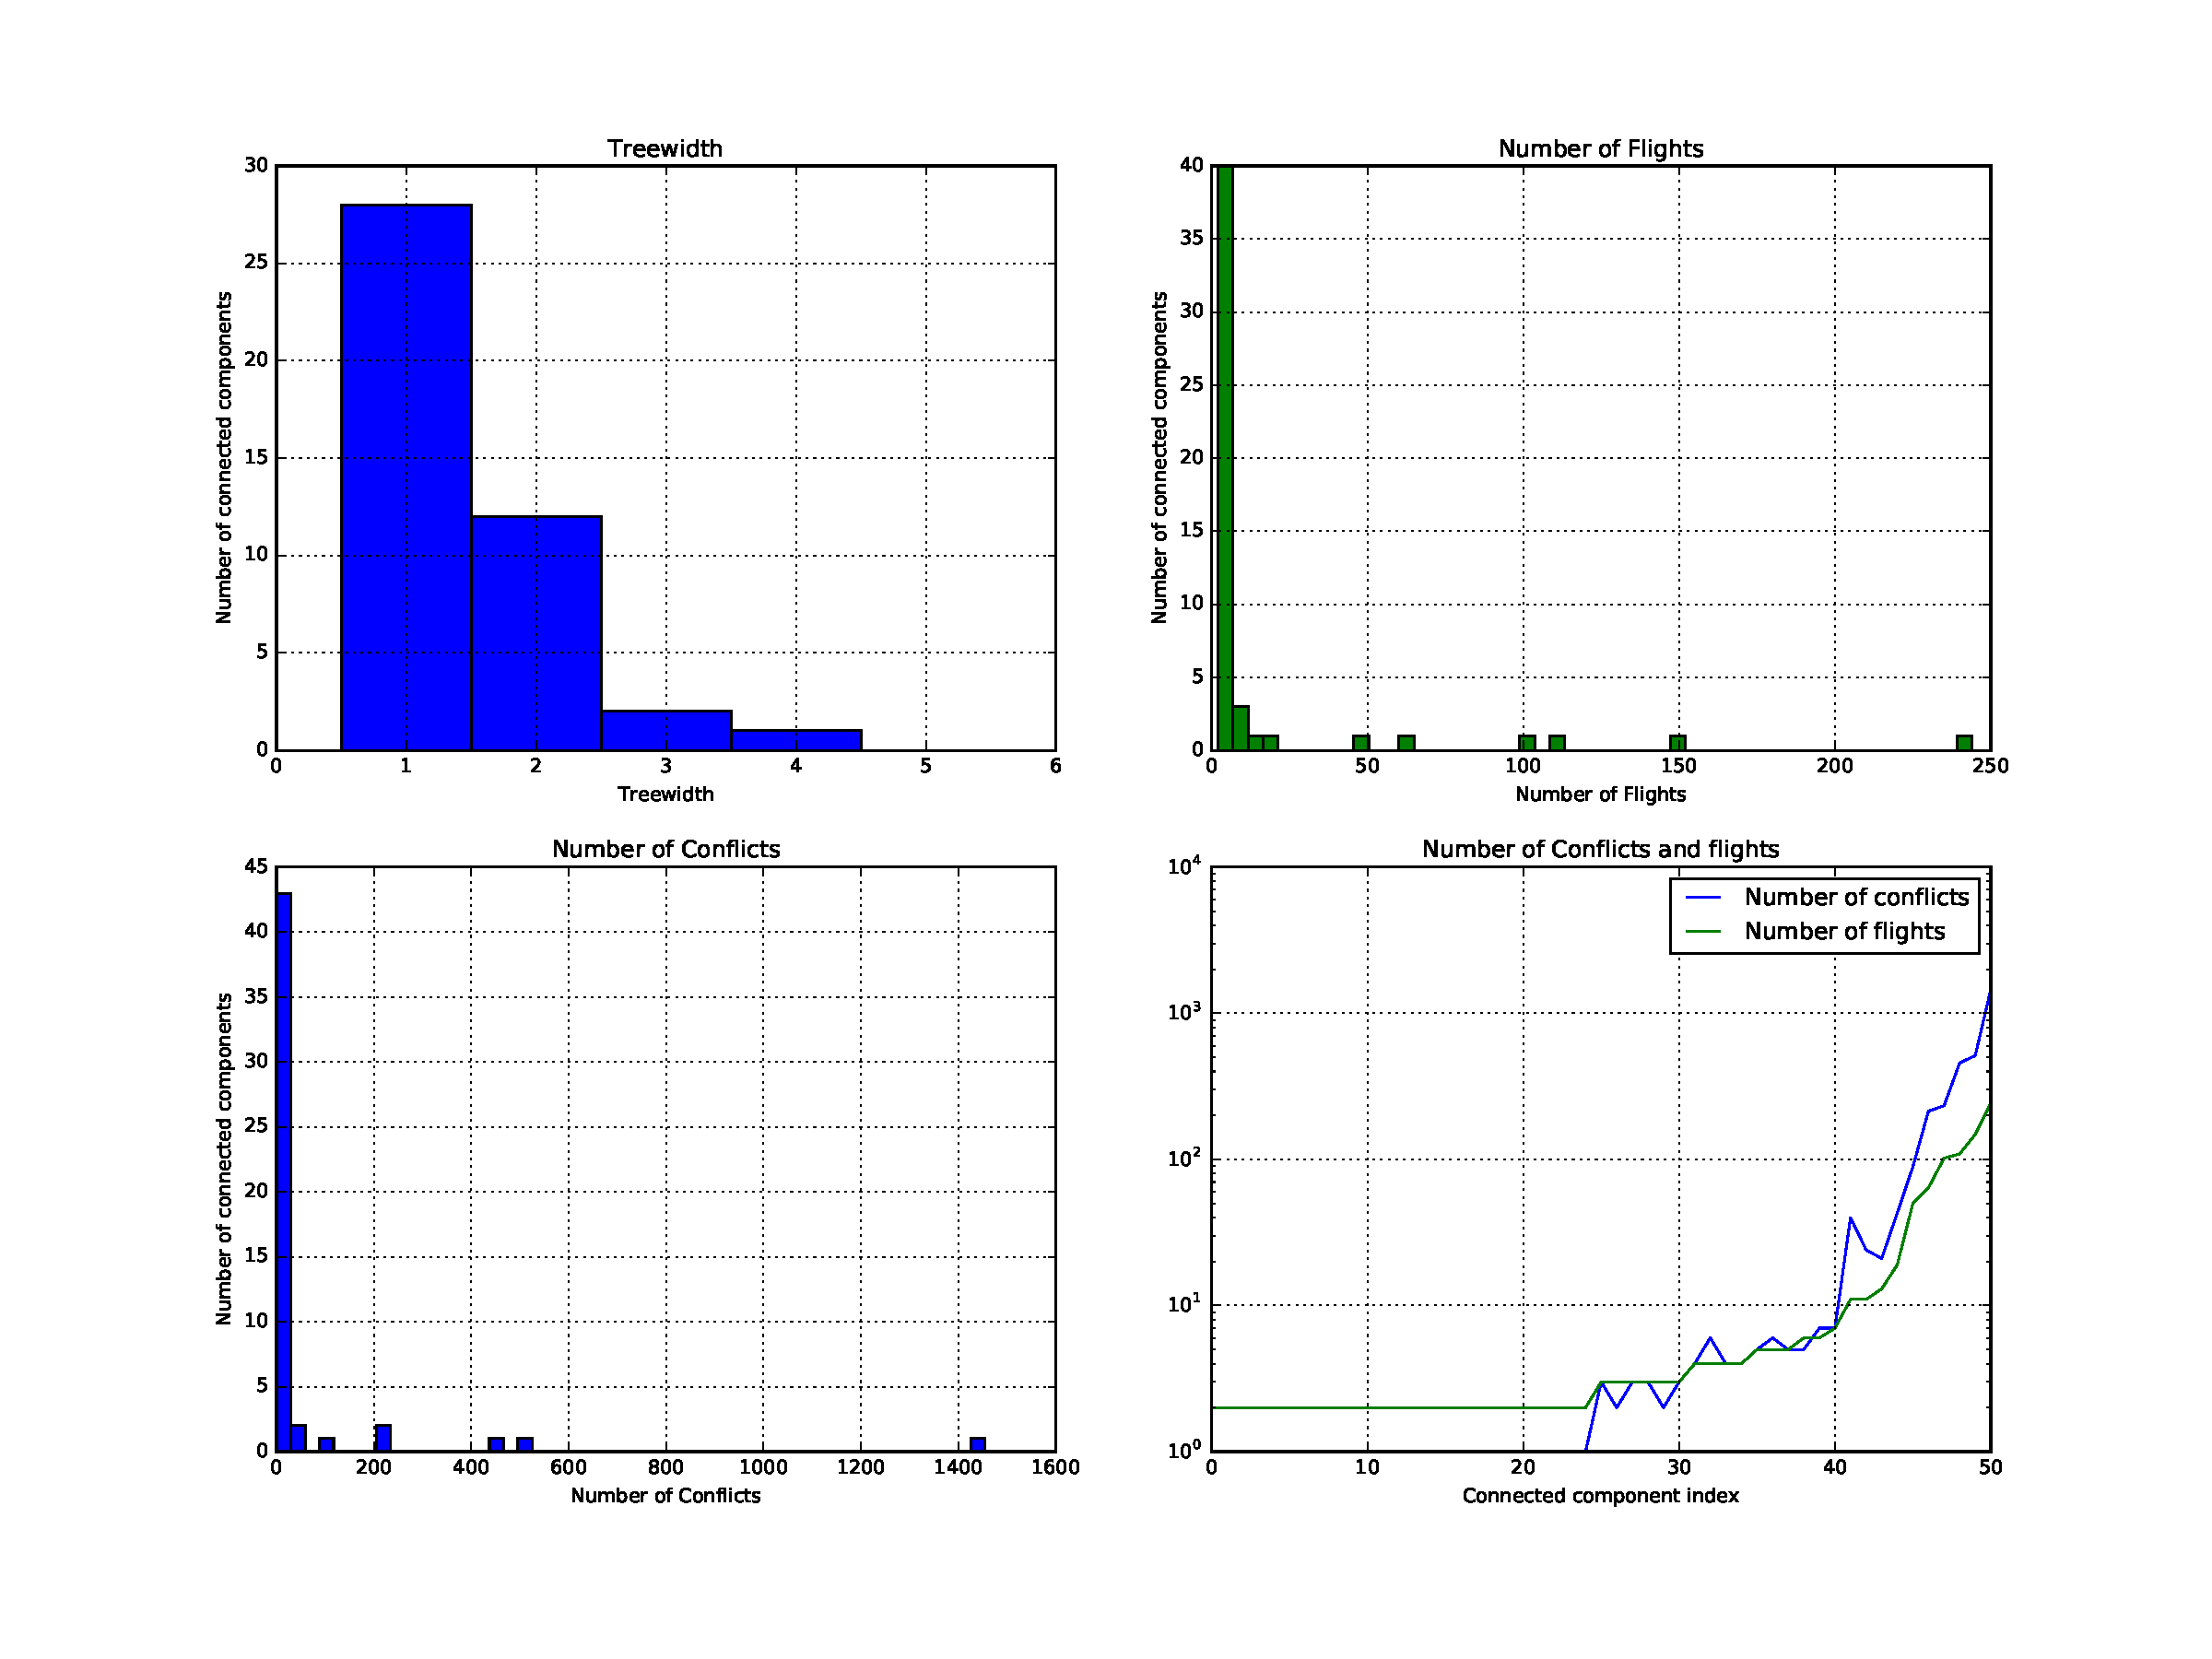
\includegraphics[width=1.0\linewidth]{pics/conflict_graph_connected_components_analysis.pdf}
    %\scalebox{0.4}{%% Creator: Matplotlib, PGF backend
%%
%% To include the figure in your LaTeX document, write
%%   \input{<filename>.pgf}
%%
%% Make sure the required packages are loaded in your preamble
%%   \usepackage{pgf}
%%
%% Figures using additional raster images can only be included by \input if
%% they are in the same directory as the main LaTeX file. For loading figures
%% from other directories you can use the `import` package
%%   \usepackage{import}
%% and then include the figures with
%%   \import{<path to file>}{<filename>.pgf}
%%
%% Matplotlib used the following preamble
%%   \usepackage{fontspec}
%%   \setmainfont{Bitstream Vera Serif}
%%   \setsansfont{Bitstream Vera Sans}
%%   \setmonofont{Bitstream Vera Sans Mono}
%%
\begingroup%
\makeatletter%
\begin{pgfpicture}%
\pgfpathrectangle{\pgfpointorigin}{\pgfqpoint{16.000000in}{12.000000in}}%
\pgfusepath{use as bounding box, clip}%
\begin{pgfscope}%
\pgfsetbuttcap%
\pgfsetmiterjoin%
\definecolor{currentfill}{rgb}{1.000000,1.000000,1.000000}%
\pgfsetfillcolor{currentfill}%
\pgfsetlinewidth{0.000000pt}%
\definecolor{currentstroke}{rgb}{1.000000,1.000000,1.000000}%
\pgfsetstrokecolor{currentstroke}%
\pgfsetdash{}{0pt}%
\pgfpathmoveto{\pgfqpoint{0.000000in}{0.000000in}}%
\pgfpathlineto{\pgfqpoint{16.000000in}{0.000000in}}%
\pgfpathlineto{\pgfqpoint{16.000000in}{12.000000in}}%
\pgfpathlineto{\pgfqpoint{0.000000in}{12.000000in}}%
\pgfpathclose%
\pgfusepath{fill}%
\end{pgfscope}%
\begin{pgfscope}%
\pgfsetbuttcap%
\pgfsetmiterjoin%
\definecolor{currentfill}{rgb}{1.000000,1.000000,1.000000}%
\pgfsetfillcolor{currentfill}%
\pgfsetlinewidth{0.000000pt}%
\definecolor{currentstroke}{rgb}{0.000000,0.000000,0.000000}%
\pgfsetstrokecolor{currentstroke}%
\pgfsetstrokeopacity{0.000000}%
\pgfsetdash{}{0pt}%
\pgfpathmoveto{\pgfqpoint{2.000000in}{6.572727in}}%
\pgfpathlineto{\pgfqpoint{7.636364in}{6.572727in}}%
\pgfpathlineto{\pgfqpoint{7.636364in}{10.800000in}}%
\pgfpathlineto{\pgfqpoint{2.000000in}{10.800000in}}%
\pgfpathclose%
\pgfusepath{fill}%
\end{pgfscope}%
\begin{pgfscope}%
\pgfpathrectangle{\pgfqpoint{2.000000in}{6.572727in}}{\pgfqpoint{5.636364in}{4.227273in}} %
\pgfusepath{clip}%
\pgfsetbuttcap%
\pgfsetmiterjoin%
\definecolor{currentfill}{rgb}{0.000000,0.000000,1.000000}%
\pgfsetfillcolor{currentfill}%
\pgfsetlinewidth{1.003750pt}%
\definecolor{currentstroke}{rgb}{0.000000,0.000000,0.000000}%
\pgfsetstrokecolor{currentstroke}%
\pgfsetdash{}{0pt}%
\pgfpathmoveto{\pgfqpoint{2.469697in}{6.572727in}}%
\pgfpathlineto{\pgfqpoint{3.409091in}{6.572727in}}%
\pgfpathlineto{\pgfqpoint{3.409091in}{10.518182in}}%
\pgfpathlineto{\pgfqpoint{2.469697in}{10.518182in}}%
\pgfpathclose%
\pgfusepath{stroke,fill}%
\end{pgfscope}%
\begin{pgfscope}%
\pgfpathrectangle{\pgfqpoint{2.000000in}{6.572727in}}{\pgfqpoint{5.636364in}{4.227273in}} %
\pgfusepath{clip}%
\pgfsetbuttcap%
\pgfsetmiterjoin%
\definecolor{currentfill}{rgb}{0.000000,0.000000,1.000000}%
\pgfsetfillcolor{currentfill}%
\pgfsetlinewidth{1.003750pt}%
\definecolor{currentstroke}{rgb}{0.000000,0.000000,0.000000}%
\pgfsetstrokecolor{currentstroke}%
\pgfsetdash{}{0pt}%
\pgfpathmoveto{\pgfqpoint{3.409091in}{6.572727in}}%
\pgfpathlineto{\pgfqpoint{4.348485in}{6.572727in}}%
\pgfpathlineto{\pgfqpoint{4.348485in}{8.263636in}}%
\pgfpathlineto{\pgfqpoint{3.409091in}{8.263636in}}%
\pgfpathclose%
\pgfusepath{stroke,fill}%
\end{pgfscope}%
\begin{pgfscope}%
\pgfpathrectangle{\pgfqpoint{2.000000in}{6.572727in}}{\pgfqpoint{5.636364in}{4.227273in}} %
\pgfusepath{clip}%
\pgfsetbuttcap%
\pgfsetmiterjoin%
\definecolor{currentfill}{rgb}{0.000000,0.000000,1.000000}%
\pgfsetfillcolor{currentfill}%
\pgfsetlinewidth{1.003750pt}%
\definecolor{currentstroke}{rgb}{0.000000,0.000000,0.000000}%
\pgfsetstrokecolor{currentstroke}%
\pgfsetdash{}{0pt}%
\pgfpathmoveto{\pgfqpoint{4.348485in}{6.572727in}}%
\pgfpathlineto{\pgfqpoint{5.287879in}{6.572727in}}%
\pgfpathlineto{\pgfqpoint{5.287879in}{6.854545in}}%
\pgfpathlineto{\pgfqpoint{4.348485in}{6.854545in}}%
\pgfpathclose%
\pgfusepath{stroke,fill}%
\end{pgfscope}%
\begin{pgfscope}%
\pgfpathrectangle{\pgfqpoint{2.000000in}{6.572727in}}{\pgfqpoint{5.636364in}{4.227273in}} %
\pgfusepath{clip}%
\pgfsetbuttcap%
\pgfsetmiterjoin%
\definecolor{currentfill}{rgb}{0.000000,0.000000,1.000000}%
\pgfsetfillcolor{currentfill}%
\pgfsetlinewidth{1.003750pt}%
\definecolor{currentstroke}{rgb}{0.000000,0.000000,0.000000}%
\pgfsetstrokecolor{currentstroke}%
\pgfsetdash{}{0pt}%
\pgfpathmoveto{\pgfqpoint{5.287879in}{6.572727in}}%
\pgfpathlineto{\pgfqpoint{6.227273in}{6.572727in}}%
\pgfpathlineto{\pgfqpoint{6.227273in}{6.713636in}}%
\pgfpathlineto{\pgfqpoint{5.287879in}{6.713636in}}%
\pgfpathclose%
\pgfusepath{stroke,fill}%
\end{pgfscope}%
\begin{pgfscope}%
\pgfpathrectangle{\pgfqpoint{2.000000in}{6.572727in}}{\pgfqpoint{5.636364in}{4.227273in}} %
\pgfusepath{clip}%
\pgfsetbuttcap%
\pgfsetmiterjoin%
\definecolor{currentfill}{rgb}{0.000000,0.000000,1.000000}%
\pgfsetfillcolor{currentfill}%
\pgfsetlinewidth{1.003750pt}%
\definecolor{currentstroke}{rgb}{0.000000,0.000000,0.000000}%
\pgfsetstrokecolor{currentstroke}%
\pgfsetdash{}{0pt}%
\pgfpathmoveto{\pgfqpoint{6.227273in}{6.572727in}}%
\pgfpathlineto{\pgfqpoint{7.166667in}{6.572727in}}%
\pgfpathlineto{\pgfqpoint{7.166667in}{6.572727in}}%
\pgfpathlineto{\pgfqpoint{6.227273in}{6.572727in}}%
\pgfpathclose%
\pgfusepath{stroke,fill}%
\end{pgfscope}%
\begin{pgfscope}%
\pgfsetrectcap%
\pgfsetmiterjoin%
\pgfsetlinewidth{1.003750pt}%
\definecolor{currentstroke}{rgb}{0.000000,0.000000,0.000000}%
\pgfsetstrokecolor{currentstroke}%
\pgfsetdash{}{0pt}%
\pgfpathmoveto{\pgfqpoint{2.000000in}{10.800000in}}%
\pgfpathlineto{\pgfqpoint{7.636364in}{10.800000in}}%
\pgfusepath{stroke}%
\end{pgfscope}%
\begin{pgfscope}%
\pgfsetrectcap%
\pgfsetmiterjoin%
\pgfsetlinewidth{1.003750pt}%
\definecolor{currentstroke}{rgb}{0.000000,0.000000,0.000000}%
\pgfsetstrokecolor{currentstroke}%
\pgfsetdash{}{0pt}%
\pgfpathmoveto{\pgfqpoint{7.636364in}{6.572727in}}%
\pgfpathlineto{\pgfqpoint{7.636364in}{10.800000in}}%
\pgfusepath{stroke}%
\end{pgfscope}%
\begin{pgfscope}%
\pgfsetrectcap%
\pgfsetmiterjoin%
\pgfsetlinewidth{1.003750pt}%
\definecolor{currentstroke}{rgb}{0.000000,0.000000,0.000000}%
\pgfsetstrokecolor{currentstroke}%
\pgfsetdash{}{0pt}%
\pgfpathmoveto{\pgfqpoint{2.000000in}{6.572727in}}%
\pgfpathlineto{\pgfqpoint{7.636364in}{6.572727in}}%
\pgfusepath{stroke}%
\end{pgfscope}%
\begin{pgfscope}%
\pgfsetrectcap%
\pgfsetmiterjoin%
\pgfsetlinewidth{1.003750pt}%
\definecolor{currentstroke}{rgb}{0.000000,0.000000,0.000000}%
\pgfsetstrokecolor{currentstroke}%
\pgfsetdash{}{0pt}%
\pgfpathmoveto{\pgfqpoint{2.000000in}{6.572727in}}%
\pgfpathlineto{\pgfqpoint{2.000000in}{10.800000in}}%
\pgfusepath{stroke}%
\end{pgfscope}%
\begin{pgfscope}%
\pgfpathrectangle{\pgfqpoint{2.000000in}{6.572727in}}{\pgfqpoint{5.636364in}{4.227273in}} %
\pgfusepath{clip}%
\pgfsetbuttcap%
\pgfsetroundjoin%
\pgfsetlinewidth{0.501875pt}%
\definecolor{currentstroke}{rgb}{0.000000,0.000000,0.000000}%
\pgfsetstrokecolor{currentstroke}%
\pgfsetdash{{1.000000pt}{3.000000pt}}{0.000000pt}%
\pgfpathmoveto{\pgfqpoint{2.000000in}{6.572727in}}%
\pgfpathlineto{\pgfqpoint{2.000000in}{10.800000in}}%
\pgfusepath{stroke}%
\end{pgfscope}%
\begin{pgfscope}%
\pgfsetbuttcap%
\pgfsetroundjoin%
\definecolor{currentfill}{rgb}{0.000000,0.000000,0.000000}%
\pgfsetfillcolor{currentfill}%
\pgfsetlinewidth{0.501875pt}%
\definecolor{currentstroke}{rgb}{0.000000,0.000000,0.000000}%
\pgfsetstrokecolor{currentstroke}%
\pgfsetdash{}{0pt}%
\pgfsys@defobject{currentmarker}{\pgfqpoint{0.000000in}{0.000000in}}{\pgfqpoint{0.000000in}{0.055556in}}{%
\pgfpathmoveto{\pgfqpoint{0.000000in}{0.000000in}}%
\pgfpathlineto{\pgfqpoint{0.000000in}{0.055556in}}%
\pgfusepath{stroke,fill}%
}%
\begin{pgfscope}%
\pgfsys@transformshift{2.000000in}{6.572727in}%
\pgfsys@useobject{currentmarker}{}%
\end{pgfscope}%
\end{pgfscope}%
\begin{pgfscope}%
\pgfsetbuttcap%
\pgfsetroundjoin%
\definecolor{currentfill}{rgb}{0.000000,0.000000,0.000000}%
\pgfsetfillcolor{currentfill}%
\pgfsetlinewidth{0.501875pt}%
\definecolor{currentstroke}{rgb}{0.000000,0.000000,0.000000}%
\pgfsetstrokecolor{currentstroke}%
\pgfsetdash{}{0pt}%
\pgfsys@defobject{currentmarker}{\pgfqpoint{0.000000in}{-0.055556in}}{\pgfqpoint{0.000000in}{0.000000in}}{%
\pgfpathmoveto{\pgfqpoint{0.000000in}{0.000000in}}%
\pgfpathlineto{\pgfqpoint{0.000000in}{-0.055556in}}%
\pgfusepath{stroke,fill}%
}%
\begin{pgfscope}%
\pgfsys@transformshift{2.000000in}{10.800000in}%
\pgfsys@useobject{currentmarker}{}%
\end{pgfscope}%
\end{pgfscope}%
\begin{pgfscope}%
\pgftext[x=2.000000in,y=6.517172in,,top]{\sffamily\fontsize{10.000000}{12.000000}\selectfont 0}%
\end{pgfscope}%
\begin{pgfscope}%
\pgfpathrectangle{\pgfqpoint{2.000000in}{6.572727in}}{\pgfqpoint{5.636364in}{4.227273in}} %
\pgfusepath{clip}%
\pgfsetbuttcap%
\pgfsetroundjoin%
\pgfsetlinewidth{0.501875pt}%
\definecolor{currentstroke}{rgb}{0.000000,0.000000,0.000000}%
\pgfsetstrokecolor{currentstroke}%
\pgfsetdash{{1.000000pt}{3.000000pt}}{0.000000pt}%
\pgfpathmoveto{\pgfqpoint{2.939394in}{6.572727in}}%
\pgfpathlineto{\pgfqpoint{2.939394in}{10.800000in}}%
\pgfusepath{stroke}%
\end{pgfscope}%
\begin{pgfscope}%
\pgfsetbuttcap%
\pgfsetroundjoin%
\definecolor{currentfill}{rgb}{0.000000,0.000000,0.000000}%
\pgfsetfillcolor{currentfill}%
\pgfsetlinewidth{0.501875pt}%
\definecolor{currentstroke}{rgb}{0.000000,0.000000,0.000000}%
\pgfsetstrokecolor{currentstroke}%
\pgfsetdash{}{0pt}%
\pgfsys@defobject{currentmarker}{\pgfqpoint{0.000000in}{0.000000in}}{\pgfqpoint{0.000000in}{0.055556in}}{%
\pgfpathmoveto{\pgfqpoint{0.000000in}{0.000000in}}%
\pgfpathlineto{\pgfqpoint{0.000000in}{0.055556in}}%
\pgfusepath{stroke,fill}%
}%
\begin{pgfscope}%
\pgfsys@transformshift{2.939394in}{6.572727in}%
\pgfsys@useobject{currentmarker}{}%
\end{pgfscope}%
\end{pgfscope}%
\begin{pgfscope}%
\pgfsetbuttcap%
\pgfsetroundjoin%
\definecolor{currentfill}{rgb}{0.000000,0.000000,0.000000}%
\pgfsetfillcolor{currentfill}%
\pgfsetlinewidth{0.501875pt}%
\definecolor{currentstroke}{rgb}{0.000000,0.000000,0.000000}%
\pgfsetstrokecolor{currentstroke}%
\pgfsetdash{}{0pt}%
\pgfsys@defobject{currentmarker}{\pgfqpoint{0.000000in}{-0.055556in}}{\pgfqpoint{0.000000in}{0.000000in}}{%
\pgfpathmoveto{\pgfqpoint{0.000000in}{0.000000in}}%
\pgfpathlineto{\pgfqpoint{0.000000in}{-0.055556in}}%
\pgfusepath{stroke,fill}%
}%
\begin{pgfscope}%
\pgfsys@transformshift{2.939394in}{10.800000in}%
\pgfsys@useobject{currentmarker}{}%
\end{pgfscope}%
\end{pgfscope}%
\begin{pgfscope}%
\pgftext[x=2.939394in,y=6.517172in,,top]{\sffamily\fontsize{10.000000}{12.000000}\selectfont 1}%
\end{pgfscope}%
\begin{pgfscope}%
\pgfpathrectangle{\pgfqpoint{2.000000in}{6.572727in}}{\pgfqpoint{5.636364in}{4.227273in}} %
\pgfusepath{clip}%
\pgfsetbuttcap%
\pgfsetroundjoin%
\pgfsetlinewidth{0.501875pt}%
\definecolor{currentstroke}{rgb}{0.000000,0.000000,0.000000}%
\pgfsetstrokecolor{currentstroke}%
\pgfsetdash{{1.000000pt}{3.000000pt}}{0.000000pt}%
\pgfpathmoveto{\pgfqpoint{3.878788in}{6.572727in}}%
\pgfpathlineto{\pgfqpoint{3.878788in}{10.800000in}}%
\pgfusepath{stroke}%
\end{pgfscope}%
\begin{pgfscope}%
\pgfsetbuttcap%
\pgfsetroundjoin%
\definecolor{currentfill}{rgb}{0.000000,0.000000,0.000000}%
\pgfsetfillcolor{currentfill}%
\pgfsetlinewidth{0.501875pt}%
\definecolor{currentstroke}{rgb}{0.000000,0.000000,0.000000}%
\pgfsetstrokecolor{currentstroke}%
\pgfsetdash{}{0pt}%
\pgfsys@defobject{currentmarker}{\pgfqpoint{0.000000in}{0.000000in}}{\pgfqpoint{0.000000in}{0.055556in}}{%
\pgfpathmoveto{\pgfqpoint{0.000000in}{0.000000in}}%
\pgfpathlineto{\pgfqpoint{0.000000in}{0.055556in}}%
\pgfusepath{stroke,fill}%
}%
\begin{pgfscope}%
\pgfsys@transformshift{3.878788in}{6.572727in}%
\pgfsys@useobject{currentmarker}{}%
\end{pgfscope}%
\end{pgfscope}%
\begin{pgfscope}%
\pgfsetbuttcap%
\pgfsetroundjoin%
\definecolor{currentfill}{rgb}{0.000000,0.000000,0.000000}%
\pgfsetfillcolor{currentfill}%
\pgfsetlinewidth{0.501875pt}%
\definecolor{currentstroke}{rgb}{0.000000,0.000000,0.000000}%
\pgfsetstrokecolor{currentstroke}%
\pgfsetdash{}{0pt}%
\pgfsys@defobject{currentmarker}{\pgfqpoint{0.000000in}{-0.055556in}}{\pgfqpoint{0.000000in}{0.000000in}}{%
\pgfpathmoveto{\pgfqpoint{0.000000in}{0.000000in}}%
\pgfpathlineto{\pgfqpoint{0.000000in}{-0.055556in}}%
\pgfusepath{stroke,fill}%
}%
\begin{pgfscope}%
\pgfsys@transformshift{3.878788in}{10.800000in}%
\pgfsys@useobject{currentmarker}{}%
\end{pgfscope}%
\end{pgfscope}%
\begin{pgfscope}%
\pgftext[x=3.878788in,y=6.517172in,,top]{\sffamily\fontsize{10.000000}{12.000000}\selectfont 2}%
\end{pgfscope}%
\begin{pgfscope}%
\pgfpathrectangle{\pgfqpoint{2.000000in}{6.572727in}}{\pgfqpoint{5.636364in}{4.227273in}} %
\pgfusepath{clip}%
\pgfsetbuttcap%
\pgfsetroundjoin%
\pgfsetlinewidth{0.501875pt}%
\definecolor{currentstroke}{rgb}{0.000000,0.000000,0.000000}%
\pgfsetstrokecolor{currentstroke}%
\pgfsetdash{{1.000000pt}{3.000000pt}}{0.000000pt}%
\pgfpathmoveto{\pgfqpoint{4.818182in}{6.572727in}}%
\pgfpathlineto{\pgfqpoint{4.818182in}{10.800000in}}%
\pgfusepath{stroke}%
\end{pgfscope}%
\begin{pgfscope}%
\pgfsetbuttcap%
\pgfsetroundjoin%
\definecolor{currentfill}{rgb}{0.000000,0.000000,0.000000}%
\pgfsetfillcolor{currentfill}%
\pgfsetlinewidth{0.501875pt}%
\definecolor{currentstroke}{rgb}{0.000000,0.000000,0.000000}%
\pgfsetstrokecolor{currentstroke}%
\pgfsetdash{}{0pt}%
\pgfsys@defobject{currentmarker}{\pgfqpoint{0.000000in}{0.000000in}}{\pgfqpoint{0.000000in}{0.055556in}}{%
\pgfpathmoveto{\pgfqpoint{0.000000in}{0.000000in}}%
\pgfpathlineto{\pgfqpoint{0.000000in}{0.055556in}}%
\pgfusepath{stroke,fill}%
}%
\begin{pgfscope}%
\pgfsys@transformshift{4.818182in}{6.572727in}%
\pgfsys@useobject{currentmarker}{}%
\end{pgfscope}%
\end{pgfscope}%
\begin{pgfscope}%
\pgfsetbuttcap%
\pgfsetroundjoin%
\definecolor{currentfill}{rgb}{0.000000,0.000000,0.000000}%
\pgfsetfillcolor{currentfill}%
\pgfsetlinewidth{0.501875pt}%
\definecolor{currentstroke}{rgb}{0.000000,0.000000,0.000000}%
\pgfsetstrokecolor{currentstroke}%
\pgfsetdash{}{0pt}%
\pgfsys@defobject{currentmarker}{\pgfqpoint{0.000000in}{-0.055556in}}{\pgfqpoint{0.000000in}{0.000000in}}{%
\pgfpathmoveto{\pgfqpoint{0.000000in}{0.000000in}}%
\pgfpathlineto{\pgfqpoint{0.000000in}{-0.055556in}}%
\pgfusepath{stroke,fill}%
}%
\begin{pgfscope}%
\pgfsys@transformshift{4.818182in}{10.800000in}%
\pgfsys@useobject{currentmarker}{}%
\end{pgfscope}%
\end{pgfscope}%
\begin{pgfscope}%
\pgftext[x=4.818182in,y=6.517172in,,top]{\sffamily\fontsize{10.000000}{12.000000}\selectfont 3}%
\end{pgfscope}%
\begin{pgfscope}%
\pgfpathrectangle{\pgfqpoint{2.000000in}{6.572727in}}{\pgfqpoint{5.636364in}{4.227273in}} %
\pgfusepath{clip}%
\pgfsetbuttcap%
\pgfsetroundjoin%
\pgfsetlinewidth{0.501875pt}%
\definecolor{currentstroke}{rgb}{0.000000,0.000000,0.000000}%
\pgfsetstrokecolor{currentstroke}%
\pgfsetdash{{1.000000pt}{3.000000pt}}{0.000000pt}%
\pgfpathmoveto{\pgfqpoint{5.757576in}{6.572727in}}%
\pgfpathlineto{\pgfqpoint{5.757576in}{10.800000in}}%
\pgfusepath{stroke}%
\end{pgfscope}%
\begin{pgfscope}%
\pgfsetbuttcap%
\pgfsetroundjoin%
\definecolor{currentfill}{rgb}{0.000000,0.000000,0.000000}%
\pgfsetfillcolor{currentfill}%
\pgfsetlinewidth{0.501875pt}%
\definecolor{currentstroke}{rgb}{0.000000,0.000000,0.000000}%
\pgfsetstrokecolor{currentstroke}%
\pgfsetdash{}{0pt}%
\pgfsys@defobject{currentmarker}{\pgfqpoint{0.000000in}{0.000000in}}{\pgfqpoint{0.000000in}{0.055556in}}{%
\pgfpathmoveto{\pgfqpoint{0.000000in}{0.000000in}}%
\pgfpathlineto{\pgfqpoint{0.000000in}{0.055556in}}%
\pgfusepath{stroke,fill}%
}%
\begin{pgfscope}%
\pgfsys@transformshift{5.757576in}{6.572727in}%
\pgfsys@useobject{currentmarker}{}%
\end{pgfscope}%
\end{pgfscope}%
\begin{pgfscope}%
\pgfsetbuttcap%
\pgfsetroundjoin%
\definecolor{currentfill}{rgb}{0.000000,0.000000,0.000000}%
\pgfsetfillcolor{currentfill}%
\pgfsetlinewidth{0.501875pt}%
\definecolor{currentstroke}{rgb}{0.000000,0.000000,0.000000}%
\pgfsetstrokecolor{currentstroke}%
\pgfsetdash{}{0pt}%
\pgfsys@defobject{currentmarker}{\pgfqpoint{0.000000in}{-0.055556in}}{\pgfqpoint{0.000000in}{0.000000in}}{%
\pgfpathmoveto{\pgfqpoint{0.000000in}{0.000000in}}%
\pgfpathlineto{\pgfqpoint{0.000000in}{-0.055556in}}%
\pgfusepath{stroke,fill}%
}%
\begin{pgfscope}%
\pgfsys@transformshift{5.757576in}{10.800000in}%
\pgfsys@useobject{currentmarker}{}%
\end{pgfscope}%
\end{pgfscope}%
\begin{pgfscope}%
\pgftext[x=5.757576in,y=6.517172in,,top]{\sffamily\fontsize{10.000000}{12.000000}\selectfont 4}%
\end{pgfscope}%
\begin{pgfscope}%
\pgfpathrectangle{\pgfqpoint{2.000000in}{6.572727in}}{\pgfqpoint{5.636364in}{4.227273in}} %
\pgfusepath{clip}%
\pgfsetbuttcap%
\pgfsetroundjoin%
\pgfsetlinewidth{0.501875pt}%
\definecolor{currentstroke}{rgb}{0.000000,0.000000,0.000000}%
\pgfsetstrokecolor{currentstroke}%
\pgfsetdash{{1.000000pt}{3.000000pt}}{0.000000pt}%
\pgfpathmoveto{\pgfqpoint{6.696970in}{6.572727in}}%
\pgfpathlineto{\pgfqpoint{6.696970in}{10.800000in}}%
\pgfusepath{stroke}%
\end{pgfscope}%
\begin{pgfscope}%
\pgfsetbuttcap%
\pgfsetroundjoin%
\definecolor{currentfill}{rgb}{0.000000,0.000000,0.000000}%
\pgfsetfillcolor{currentfill}%
\pgfsetlinewidth{0.501875pt}%
\definecolor{currentstroke}{rgb}{0.000000,0.000000,0.000000}%
\pgfsetstrokecolor{currentstroke}%
\pgfsetdash{}{0pt}%
\pgfsys@defobject{currentmarker}{\pgfqpoint{0.000000in}{0.000000in}}{\pgfqpoint{0.000000in}{0.055556in}}{%
\pgfpathmoveto{\pgfqpoint{0.000000in}{0.000000in}}%
\pgfpathlineto{\pgfqpoint{0.000000in}{0.055556in}}%
\pgfusepath{stroke,fill}%
}%
\begin{pgfscope}%
\pgfsys@transformshift{6.696970in}{6.572727in}%
\pgfsys@useobject{currentmarker}{}%
\end{pgfscope}%
\end{pgfscope}%
\begin{pgfscope}%
\pgfsetbuttcap%
\pgfsetroundjoin%
\definecolor{currentfill}{rgb}{0.000000,0.000000,0.000000}%
\pgfsetfillcolor{currentfill}%
\pgfsetlinewidth{0.501875pt}%
\definecolor{currentstroke}{rgb}{0.000000,0.000000,0.000000}%
\pgfsetstrokecolor{currentstroke}%
\pgfsetdash{}{0pt}%
\pgfsys@defobject{currentmarker}{\pgfqpoint{0.000000in}{-0.055556in}}{\pgfqpoint{0.000000in}{0.000000in}}{%
\pgfpathmoveto{\pgfqpoint{0.000000in}{0.000000in}}%
\pgfpathlineto{\pgfqpoint{0.000000in}{-0.055556in}}%
\pgfusepath{stroke,fill}%
}%
\begin{pgfscope}%
\pgfsys@transformshift{6.696970in}{10.800000in}%
\pgfsys@useobject{currentmarker}{}%
\end{pgfscope}%
\end{pgfscope}%
\begin{pgfscope}%
\pgftext[x=6.696970in,y=6.517172in,,top]{\sffamily\fontsize{10.000000}{12.000000}\selectfont 5}%
\end{pgfscope}%
\begin{pgfscope}%
\pgfpathrectangle{\pgfqpoint{2.000000in}{6.572727in}}{\pgfqpoint{5.636364in}{4.227273in}} %
\pgfusepath{clip}%
\pgfsetbuttcap%
\pgfsetroundjoin%
\pgfsetlinewidth{0.501875pt}%
\definecolor{currentstroke}{rgb}{0.000000,0.000000,0.000000}%
\pgfsetstrokecolor{currentstroke}%
\pgfsetdash{{1.000000pt}{3.000000pt}}{0.000000pt}%
\pgfpathmoveto{\pgfqpoint{7.636364in}{6.572727in}}%
\pgfpathlineto{\pgfqpoint{7.636364in}{10.800000in}}%
\pgfusepath{stroke}%
\end{pgfscope}%
\begin{pgfscope}%
\pgfsetbuttcap%
\pgfsetroundjoin%
\definecolor{currentfill}{rgb}{0.000000,0.000000,0.000000}%
\pgfsetfillcolor{currentfill}%
\pgfsetlinewidth{0.501875pt}%
\definecolor{currentstroke}{rgb}{0.000000,0.000000,0.000000}%
\pgfsetstrokecolor{currentstroke}%
\pgfsetdash{}{0pt}%
\pgfsys@defobject{currentmarker}{\pgfqpoint{0.000000in}{0.000000in}}{\pgfqpoint{0.000000in}{0.055556in}}{%
\pgfpathmoveto{\pgfqpoint{0.000000in}{0.000000in}}%
\pgfpathlineto{\pgfqpoint{0.000000in}{0.055556in}}%
\pgfusepath{stroke,fill}%
}%
\begin{pgfscope}%
\pgfsys@transformshift{7.636364in}{6.572727in}%
\pgfsys@useobject{currentmarker}{}%
\end{pgfscope}%
\end{pgfscope}%
\begin{pgfscope}%
\pgfsetbuttcap%
\pgfsetroundjoin%
\definecolor{currentfill}{rgb}{0.000000,0.000000,0.000000}%
\pgfsetfillcolor{currentfill}%
\pgfsetlinewidth{0.501875pt}%
\definecolor{currentstroke}{rgb}{0.000000,0.000000,0.000000}%
\pgfsetstrokecolor{currentstroke}%
\pgfsetdash{}{0pt}%
\pgfsys@defobject{currentmarker}{\pgfqpoint{0.000000in}{-0.055556in}}{\pgfqpoint{0.000000in}{0.000000in}}{%
\pgfpathmoveto{\pgfqpoint{0.000000in}{0.000000in}}%
\pgfpathlineto{\pgfqpoint{0.000000in}{-0.055556in}}%
\pgfusepath{stroke,fill}%
}%
\begin{pgfscope}%
\pgfsys@transformshift{7.636364in}{10.800000in}%
\pgfsys@useobject{currentmarker}{}%
\end{pgfscope}%
\end{pgfscope}%
\begin{pgfscope}%
\pgftext[x=7.636364in,y=6.517172in,,top]{\sffamily\fontsize{10.000000}{12.000000}\selectfont 6}%
\end{pgfscope}%
\begin{pgfscope}%
\pgftext[x=4.818182in,y=6.313314in,,top]{\sffamily\fontsize{10.000000}{12.000000}\selectfont Treewidth}%
\end{pgfscope}%
\begin{pgfscope}%
\pgfpathrectangle{\pgfqpoint{2.000000in}{6.572727in}}{\pgfqpoint{5.636364in}{4.227273in}} %
\pgfusepath{clip}%
\pgfsetbuttcap%
\pgfsetroundjoin%
\pgfsetlinewidth{0.501875pt}%
\definecolor{currentstroke}{rgb}{0.000000,0.000000,0.000000}%
\pgfsetstrokecolor{currentstroke}%
\pgfsetdash{{1.000000pt}{3.000000pt}}{0.000000pt}%
\pgfpathmoveto{\pgfqpoint{2.000000in}{6.572727in}}%
\pgfpathlineto{\pgfqpoint{7.636364in}{6.572727in}}%
\pgfusepath{stroke}%
\end{pgfscope}%
\begin{pgfscope}%
\pgfsetbuttcap%
\pgfsetroundjoin%
\definecolor{currentfill}{rgb}{0.000000,0.000000,0.000000}%
\pgfsetfillcolor{currentfill}%
\pgfsetlinewidth{0.501875pt}%
\definecolor{currentstroke}{rgb}{0.000000,0.000000,0.000000}%
\pgfsetstrokecolor{currentstroke}%
\pgfsetdash{}{0pt}%
\pgfsys@defobject{currentmarker}{\pgfqpoint{0.000000in}{0.000000in}}{\pgfqpoint{0.055556in}{0.000000in}}{%
\pgfpathmoveto{\pgfqpoint{0.000000in}{0.000000in}}%
\pgfpathlineto{\pgfqpoint{0.055556in}{0.000000in}}%
\pgfusepath{stroke,fill}%
}%
\begin{pgfscope}%
\pgfsys@transformshift{2.000000in}{6.572727in}%
\pgfsys@useobject{currentmarker}{}%
\end{pgfscope}%
\end{pgfscope}%
\begin{pgfscope}%
\pgfsetbuttcap%
\pgfsetroundjoin%
\definecolor{currentfill}{rgb}{0.000000,0.000000,0.000000}%
\pgfsetfillcolor{currentfill}%
\pgfsetlinewidth{0.501875pt}%
\definecolor{currentstroke}{rgb}{0.000000,0.000000,0.000000}%
\pgfsetstrokecolor{currentstroke}%
\pgfsetdash{}{0pt}%
\pgfsys@defobject{currentmarker}{\pgfqpoint{-0.055556in}{0.000000in}}{\pgfqpoint{0.000000in}{0.000000in}}{%
\pgfpathmoveto{\pgfqpoint{0.000000in}{0.000000in}}%
\pgfpathlineto{\pgfqpoint{-0.055556in}{0.000000in}}%
\pgfusepath{stroke,fill}%
}%
\begin{pgfscope}%
\pgfsys@transformshift{7.636364in}{6.572727in}%
\pgfsys@useobject{currentmarker}{}%
\end{pgfscope}%
\end{pgfscope}%
\begin{pgfscope}%
\pgftext[x=1.944444in,y=6.572727in,right,]{\sffamily\fontsize{10.000000}{12.000000}\selectfont 0}%
\end{pgfscope}%
\begin{pgfscope}%
\pgfpathrectangle{\pgfqpoint{2.000000in}{6.572727in}}{\pgfqpoint{5.636364in}{4.227273in}} %
\pgfusepath{clip}%
\pgfsetbuttcap%
\pgfsetroundjoin%
\pgfsetlinewidth{0.501875pt}%
\definecolor{currentstroke}{rgb}{0.000000,0.000000,0.000000}%
\pgfsetstrokecolor{currentstroke}%
\pgfsetdash{{1.000000pt}{3.000000pt}}{0.000000pt}%
\pgfpathmoveto{\pgfqpoint{2.000000in}{7.277273in}}%
\pgfpathlineto{\pgfqpoint{7.636364in}{7.277273in}}%
\pgfusepath{stroke}%
\end{pgfscope}%
\begin{pgfscope}%
\pgfsetbuttcap%
\pgfsetroundjoin%
\definecolor{currentfill}{rgb}{0.000000,0.000000,0.000000}%
\pgfsetfillcolor{currentfill}%
\pgfsetlinewidth{0.501875pt}%
\definecolor{currentstroke}{rgb}{0.000000,0.000000,0.000000}%
\pgfsetstrokecolor{currentstroke}%
\pgfsetdash{}{0pt}%
\pgfsys@defobject{currentmarker}{\pgfqpoint{0.000000in}{0.000000in}}{\pgfqpoint{0.055556in}{0.000000in}}{%
\pgfpathmoveto{\pgfqpoint{0.000000in}{0.000000in}}%
\pgfpathlineto{\pgfqpoint{0.055556in}{0.000000in}}%
\pgfusepath{stroke,fill}%
}%
\begin{pgfscope}%
\pgfsys@transformshift{2.000000in}{7.277273in}%
\pgfsys@useobject{currentmarker}{}%
\end{pgfscope}%
\end{pgfscope}%
\begin{pgfscope}%
\pgfsetbuttcap%
\pgfsetroundjoin%
\definecolor{currentfill}{rgb}{0.000000,0.000000,0.000000}%
\pgfsetfillcolor{currentfill}%
\pgfsetlinewidth{0.501875pt}%
\definecolor{currentstroke}{rgb}{0.000000,0.000000,0.000000}%
\pgfsetstrokecolor{currentstroke}%
\pgfsetdash{}{0pt}%
\pgfsys@defobject{currentmarker}{\pgfqpoint{-0.055556in}{0.000000in}}{\pgfqpoint{0.000000in}{0.000000in}}{%
\pgfpathmoveto{\pgfqpoint{0.000000in}{0.000000in}}%
\pgfpathlineto{\pgfqpoint{-0.055556in}{0.000000in}}%
\pgfusepath{stroke,fill}%
}%
\begin{pgfscope}%
\pgfsys@transformshift{7.636364in}{7.277273in}%
\pgfsys@useobject{currentmarker}{}%
\end{pgfscope}%
\end{pgfscope}%
\begin{pgfscope}%
\pgftext[x=1.944444in,y=7.277273in,right,]{\sffamily\fontsize{10.000000}{12.000000}\selectfont 5}%
\end{pgfscope}%
\begin{pgfscope}%
\pgfpathrectangle{\pgfqpoint{2.000000in}{6.572727in}}{\pgfqpoint{5.636364in}{4.227273in}} %
\pgfusepath{clip}%
\pgfsetbuttcap%
\pgfsetroundjoin%
\pgfsetlinewidth{0.501875pt}%
\definecolor{currentstroke}{rgb}{0.000000,0.000000,0.000000}%
\pgfsetstrokecolor{currentstroke}%
\pgfsetdash{{1.000000pt}{3.000000pt}}{0.000000pt}%
\pgfpathmoveto{\pgfqpoint{2.000000in}{7.981818in}}%
\pgfpathlineto{\pgfqpoint{7.636364in}{7.981818in}}%
\pgfusepath{stroke}%
\end{pgfscope}%
\begin{pgfscope}%
\pgfsetbuttcap%
\pgfsetroundjoin%
\definecolor{currentfill}{rgb}{0.000000,0.000000,0.000000}%
\pgfsetfillcolor{currentfill}%
\pgfsetlinewidth{0.501875pt}%
\definecolor{currentstroke}{rgb}{0.000000,0.000000,0.000000}%
\pgfsetstrokecolor{currentstroke}%
\pgfsetdash{}{0pt}%
\pgfsys@defobject{currentmarker}{\pgfqpoint{0.000000in}{0.000000in}}{\pgfqpoint{0.055556in}{0.000000in}}{%
\pgfpathmoveto{\pgfqpoint{0.000000in}{0.000000in}}%
\pgfpathlineto{\pgfqpoint{0.055556in}{0.000000in}}%
\pgfusepath{stroke,fill}%
}%
\begin{pgfscope}%
\pgfsys@transformshift{2.000000in}{7.981818in}%
\pgfsys@useobject{currentmarker}{}%
\end{pgfscope}%
\end{pgfscope}%
\begin{pgfscope}%
\pgfsetbuttcap%
\pgfsetroundjoin%
\definecolor{currentfill}{rgb}{0.000000,0.000000,0.000000}%
\pgfsetfillcolor{currentfill}%
\pgfsetlinewidth{0.501875pt}%
\definecolor{currentstroke}{rgb}{0.000000,0.000000,0.000000}%
\pgfsetstrokecolor{currentstroke}%
\pgfsetdash{}{0pt}%
\pgfsys@defobject{currentmarker}{\pgfqpoint{-0.055556in}{0.000000in}}{\pgfqpoint{0.000000in}{0.000000in}}{%
\pgfpathmoveto{\pgfqpoint{0.000000in}{0.000000in}}%
\pgfpathlineto{\pgfqpoint{-0.055556in}{0.000000in}}%
\pgfusepath{stroke,fill}%
}%
\begin{pgfscope}%
\pgfsys@transformshift{7.636364in}{7.981818in}%
\pgfsys@useobject{currentmarker}{}%
\end{pgfscope}%
\end{pgfscope}%
\begin{pgfscope}%
\pgftext[x=1.944444in,y=7.981818in,right,]{\sffamily\fontsize{10.000000}{12.000000}\selectfont 10}%
\end{pgfscope}%
\begin{pgfscope}%
\pgfpathrectangle{\pgfqpoint{2.000000in}{6.572727in}}{\pgfqpoint{5.636364in}{4.227273in}} %
\pgfusepath{clip}%
\pgfsetbuttcap%
\pgfsetroundjoin%
\pgfsetlinewidth{0.501875pt}%
\definecolor{currentstroke}{rgb}{0.000000,0.000000,0.000000}%
\pgfsetstrokecolor{currentstroke}%
\pgfsetdash{{1.000000pt}{3.000000pt}}{0.000000pt}%
\pgfpathmoveto{\pgfqpoint{2.000000in}{8.686364in}}%
\pgfpathlineto{\pgfqpoint{7.636364in}{8.686364in}}%
\pgfusepath{stroke}%
\end{pgfscope}%
\begin{pgfscope}%
\pgfsetbuttcap%
\pgfsetroundjoin%
\definecolor{currentfill}{rgb}{0.000000,0.000000,0.000000}%
\pgfsetfillcolor{currentfill}%
\pgfsetlinewidth{0.501875pt}%
\definecolor{currentstroke}{rgb}{0.000000,0.000000,0.000000}%
\pgfsetstrokecolor{currentstroke}%
\pgfsetdash{}{0pt}%
\pgfsys@defobject{currentmarker}{\pgfqpoint{0.000000in}{0.000000in}}{\pgfqpoint{0.055556in}{0.000000in}}{%
\pgfpathmoveto{\pgfqpoint{0.000000in}{0.000000in}}%
\pgfpathlineto{\pgfqpoint{0.055556in}{0.000000in}}%
\pgfusepath{stroke,fill}%
}%
\begin{pgfscope}%
\pgfsys@transformshift{2.000000in}{8.686364in}%
\pgfsys@useobject{currentmarker}{}%
\end{pgfscope}%
\end{pgfscope}%
\begin{pgfscope}%
\pgfsetbuttcap%
\pgfsetroundjoin%
\definecolor{currentfill}{rgb}{0.000000,0.000000,0.000000}%
\pgfsetfillcolor{currentfill}%
\pgfsetlinewidth{0.501875pt}%
\definecolor{currentstroke}{rgb}{0.000000,0.000000,0.000000}%
\pgfsetstrokecolor{currentstroke}%
\pgfsetdash{}{0pt}%
\pgfsys@defobject{currentmarker}{\pgfqpoint{-0.055556in}{0.000000in}}{\pgfqpoint{0.000000in}{0.000000in}}{%
\pgfpathmoveto{\pgfqpoint{0.000000in}{0.000000in}}%
\pgfpathlineto{\pgfqpoint{-0.055556in}{0.000000in}}%
\pgfusepath{stroke,fill}%
}%
\begin{pgfscope}%
\pgfsys@transformshift{7.636364in}{8.686364in}%
\pgfsys@useobject{currentmarker}{}%
\end{pgfscope}%
\end{pgfscope}%
\begin{pgfscope}%
\pgftext[x=1.944444in,y=8.686364in,right,]{\sffamily\fontsize{10.000000}{12.000000}\selectfont 15}%
\end{pgfscope}%
\begin{pgfscope}%
\pgfpathrectangle{\pgfqpoint{2.000000in}{6.572727in}}{\pgfqpoint{5.636364in}{4.227273in}} %
\pgfusepath{clip}%
\pgfsetbuttcap%
\pgfsetroundjoin%
\pgfsetlinewidth{0.501875pt}%
\definecolor{currentstroke}{rgb}{0.000000,0.000000,0.000000}%
\pgfsetstrokecolor{currentstroke}%
\pgfsetdash{{1.000000pt}{3.000000pt}}{0.000000pt}%
\pgfpathmoveto{\pgfqpoint{2.000000in}{9.390909in}}%
\pgfpathlineto{\pgfqpoint{7.636364in}{9.390909in}}%
\pgfusepath{stroke}%
\end{pgfscope}%
\begin{pgfscope}%
\pgfsetbuttcap%
\pgfsetroundjoin%
\definecolor{currentfill}{rgb}{0.000000,0.000000,0.000000}%
\pgfsetfillcolor{currentfill}%
\pgfsetlinewidth{0.501875pt}%
\definecolor{currentstroke}{rgb}{0.000000,0.000000,0.000000}%
\pgfsetstrokecolor{currentstroke}%
\pgfsetdash{}{0pt}%
\pgfsys@defobject{currentmarker}{\pgfqpoint{0.000000in}{0.000000in}}{\pgfqpoint{0.055556in}{0.000000in}}{%
\pgfpathmoveto{\pgfqpoint{0.000000in}{0.000000in}}%
\pgfpathlineto{\pgfqpoint{0.055556in}{0.000000in}}%
\pgfusepath{stroke,fill}%
}%
\begin{pgfscope}%
\pgfsys@transformshift{2.000000in}{9.390909in}%
\pgfsys@useobject{currentmarker}{}%
\end{pgfscope}%
\end{pgfscope}%
\begin{pgfscope}%
\pgfsetbuttcap%
\pgfsetroundjoin%
\definecolor{currentfill}{rgb}{0.000000,0.000000,0.000000}%
\pgfsetfillcolor{currentfill}%
\pgfsetlinewidth{0.501875pt}%
\definecolor{currentstroke}{rgb}{0.000000,0.000000,0.000000}%
\pgfsetstrokecolor{currentstroke}%
\pgfsetdash{}{0pt}%
\pgfsys@defobject{currentmarker}{\pgfqpoint{-0.055556in}{0.000000in}}{\pgfqpoint{0.000000in}{0.000000in}}{%
\pgfpathmoveto{\pgfqpoint{0.000000in}{0.000000in}}%
\pgfpathlineto{\pgfqpoint{-0.055556in}{0.000000in}}%
\pgfusepath{stroke,fill}%
}%
\begin{pgfscope}%
\pgfsys@transformshift{7.636364in}{9.390909in}%
\pgfsys@useobject{currentmarker}{}%
\end{pgfscope}%
\end{pgfscope}%
\begin{pgfscope}%
\pgftext[x=1.944444in,y=9.390909in,right,]{\sffamily\fontsize{10.000000}{12.000000}\selectfont 20}%
\end{pgfscope}%
\begin{pgfscope}%
\pgfpathrectangle{\pgfqpoint{2.000000in}{6.572727in}}{\pgfqpoint{5.636364in}{4.227273in}} %
\pgfusepath{clip}%
\pgfsetbuttcap%
\pgfsetroundjoin%
\pgfsetlinewidth{0.501875pt}%
\definecolor{currentstroke}{rgb}{0.000000,0.000000,0.000000}%
\pgfsetstrokecolor{currentstroke}%
\pgfsetdash{{1.000000pt}{3.000000pt}}{0.000000pt}%
\pgfpathmoveto{\pgfqpoint{2.000000in}{10.095455in}}%
\pgfpathlineto{\pgfqpoint{7.636364in}{10.095455in}}%
\pgfusepath{stroke}%
\end{pgfscope}%
\begin{pgfscope}%
\pgfsetbuttcap%
\pgfsetroundjoin%
\definecolor{currentfill}{rgb}{0.000000,0.000000,0.000000}%
\pgfsetfillcolor{currentfill}%
\pgfsetlinewidth{0.501875pt}%
\definecolor{currentstroke}{rgb}{0.000000,0.000000,0.000000}%
\pgfsetstrokecolor{currentstroke}%
\pgfsetdash{}{0pt}%
\pgfsys@defobject{currentmarker}{\pgfqpoint{0.000000in}{0.000000in}}{\pgfqpoint{0.055556in}{0.000000in}}{%
\pgfpathmoveto{\pgfqpoint{0.000000in}{0.000000in}}%
\pgfpathlineto{\pgfqpoint{0.055556in}{0.000000in}}%
\pgfusepath{stroke,fill}%
}%
\begin{pgfscope}%
\pgfsys@transformshift{2.000000in}{10.095455in}%
\pgfsys@useobject{currentmarker}{}%
\end{pgfscope}%
\end{pgfscope}%
\begin{pgfscope}%
\pgfsetbuttcap%
\pgfsetroundjoin%
\definecolor{currentfill}{rgb}{0.000000,0.000000,0.000000}%
\pgfsetfillcolor{currentfill}%
\pgfsetlinewidth{0.501875pt}%
\definecolor{currentstroke}{rgb}{0.000000,0.000000,0.000000}%
\pgfsetstrokecolor{currentstroke}%
\pgfsetdash{}{0pt}%
\pgfsys@defobject{currentmarker}{\pgfqpoint{-0.055556in}{0.000000in}}{\pgfqpoint{0.000000in}{0.000000in}}{%
\pgfpathmoveto{\pgfqpoint{0.000000in}{0.000000in}}%
\pgfpathlineto{\pgfqpoint{-0.055556in}{0.000000in}}%
\pgfusepath{stroke,fill}%
}%
\begin{pgfscope}%
\pgfsys@transformshift{7.636364in}{10.095455in}%
\pgfsys@useobject{currentmarker}{}%
\end{pgfscope}%
\end{pgfscope}%
\begin{pgfscope}%
\pgftext[x=1.944444in,y=10.095455in,right,]{\sffamily\fontsize{10.000000}{12.000000}\selectfont 25}%
\end{pgfscope}%
\begin{pgfscope}%
\pgfpathrectangle{\pgfqpoint{2.000000in}{6.572727in}}{\pgfqpoint{5.636364in}{4.227273in}} %
\pgfusepath{clip}%
\pgfsetbuttcap%
\pgfsetroundjoin%
\pgfsetlinewidth{0.501875pt}%
\definecolor{currentstroke}{rgb}{0.000000,0.000000,0.000000}%
\pgfsetstrokecolor{currentstroke}%
\pgfsetdash{{1.000000pt}{3.000000pt}}{0.000000pt}%
\pgfpathmoveto{\pgfqpoint{2.000000in}{10.800000in}}%
\pgfpathlineto{\pgfqpoint{7.636364in}{10.800000in}}%
\pgfusepath{stroke}%
\end{pgfscope}%
\begin{pgfscope}%
\pgfsetbuttcap%
\pgfsetroundjoin%
\definecolor{currentfill}{rgb}{0.000000,0.000000,0.000000}%
\pgfsetfillcolor{currentfill}%
\pgfsetlinewidth{0.501875pt}%
\definecolor{currentstroke}{rgb}{0.000000,0.000000,0.000000}%
\pgfsetstrokecolor{currentstroke}%
\pgfsetdash{}{0pt}%
\pgfsys@defobject{currentmarker}{\pgfqpoint{0.000000in}{0.000000in}}{\pgfqpoint{0.055556in}{0.000000in}}{%
\pgfpathmoveto{\pgfqpoint{0.000000in}{0.000000in}}%
\pgfpathlineto{\pgfqpoint{0.055556in}{0.000000in}}%
\pgfusepath{stroke,fill}%
}%
\begin{pgfscope}%
\pgfsys@transformshift{2.000000in}{10.800000in}%
\pgfsys@useobject{currentmarker}{}%
\end{pgfscope}%
\end{pgfscope}%
\begin{pgfscope}%
\pgfsetbuttcap%
\pgfsetroundjoin%
\definecolor{currentfill}{rgb}{0.000000,0.000000,0.000000}%
\pgfsetfillcolor{currentfill}%
\pgfsetlinewidth{0.501875pt}%
\definecolor{currentstroke}{rgb}{0.000000,0.000000,0.000000}%
\pgfsetstrokecolor{currentstroke}%
\pgfsetdash{}{0pt}%
\pgfsys@defobject{currentmarker}{\pgfqpoint{-0.055556in}{0.000000in}}{\pgfqpoint{0.000000in}{0.000000in}}{%
\pgfpathmoveto{\pgfqpoint{0.000000in}{0.000000in}}%
\pgfpathlineto{\pgfqpoint{-0.055556in}{0.000000in}}%
\pgfusepath{stroke,fill}%
}%
\begin{pgfscope}%
\pgfsys@transformshift{7.636364in}{10.800000in}%
\pgfsys@useobject{currentmarker}{}%
\end{pgfscope}%
\end{pgfscope}%
\begin{pgfscope}%
\pgftext[x=1.944444in,y=10.800000in,right,]{\sffamily\fontsize{10.000000}{12.000000}\selectfont 30}%
\end{pgfscope}%
\begin{pgfscope}%
\pgftext[x=1.698269in,y=8.686364in,,bottom,rotate=90.000000]{\sffamily\fontsize{10.000000}{12.000000}\selectfont Number of connected components}%
\end{pgfscope}%
\begin{pgfscope}%
\pgftext[x=4.818182in,y=10.869444in,,base]{\sffamily\fontsize{12.000000}{14.400000}\selectfont Treewidth}%
\end{pgfscope}%
\begin{pgfscope}%
\pgfsetbuttcap%
\pgfsetmiterjoin%
\definecolor{currentfill}{rgb}{1.000000,1.000000,1.000000}%
\pgfsetfillcolor{currentfill}%
\pgfsetlinewidth{0.000000pt}%
\definecolor{currentstroke}{rgb}{0.000000,0.000000,0.000000}%
\pgfsetstrokecolor{currentstroke}%
\pgfsetstrokeopacity{0.000000}%
\pgfsetdash{}{0pt}%
\pgfpathmoveto{\pgfqpoint{8.763636in}{6.572727in}}%
\pgfpathlineto{\pgfqpoint{14.400000in}{6.572727in}}%
\pgfpathlineto{\pgfqpoint{14.400000in}{10.800000in}}%
\pgfpathlineto{\pgfqpoint{8.763636in}{10.800000in}}%
\pgfpathclose%
\pgfusepath{fill}%
\end{pgfscope}%
\begin{pgfscope}%
\pgfpathrectangle{\pgfqpoint{8.763636in}{6.572727in}}{\pgfqpoint{5.636364in}{4.227273in}} %
\pgfusepath{clip}%
\pgfsetbuttcap%
\pgfsetmiterjoin%
\definecolor{currentfill}{rgb}{0.000000,0.500000,0.000000}%
\pgfsetfillcolor{currentfill}%
\pgfsetlinewidth{1.003750pt}%
\definecolor{currentstroke}{rgb}{0.000000,0.000000,0.000000}%
\pgfsetstrokecolor{currentstroke}%
\pgfsetdash{}{0pt}%
\pgfpathmoveto{\pgfqpoint{8.808727in}{6.572727in}}%
\pgfpathlineto{\pgfqpoint{8.917847in}{6.572727in}}%
\pgfpathlineto{\pgfqpoint{8.917847in}{10.800000in}}%
\pgfpathlineto{\pgfqpoint{8.808727in}{10.800000in}}%
\pgfpathclose%
\pgfusepath{stroke,fill}%
\end{pgfscope}%
\begin{pgfscope}%
\pgfpathrectangle{\pgfqpoint{8.763636in}{6.572727in}}{\pgfqpoint{5.636364in}{4.227273in}} %
\pgfusepath{clip}%
\pgfsetbuttcap%
\pgfsetmiterjoin%
\definecolor{currentfill}{rgb}{0.000000,0.500000,0.000000}%
\pgfsetfillcolor{currentfill}%
\pgfsetlinewidth{1.003750pt}%
\definecolor{currentstroke}{rgb}{0.000000,0.000000,0.000000}%
\pgfsetstrokecolor{currentstroke}%
\pgfsetdash{}{0pt}%
\pgfpathmoveto{\pgfqpoint{8.917847in}{6.572727in}}%
\pgfpathlineto{\pgfqpoint{9.026967in}{6.572727in}}%
\pgfpathlineto{\pgfqpoint{9.026967in}{6.889773in}}%
\pgfpathlineto{\pgfqpoint{8.917847in}{6.889773in}}%
\pgfpathclose%
\pgfusepath{stroke,fill}%
\end{pgfscope}%
\begin{pgfscope}%
\pgfpathrectangle{\pgfqpoint{8.763636in}{6.572727in}}{\pgfqpoint{5.636364in}{4.227273in}} %
\pgfusepath{clip}%
\pgfsetbuttcap%
\pgfsetmiterjoin%
\definecolor{currentfill}{rgb}{0.000000,0.500000,0.000000}%
\pgfsetfillcolor{currentfill}%
\pgfsetlinewidth{1.003750pt}%
\definecolor{currentstroke}{rgb}{0.000000,0.000000,0.000000}%
\pgfsetstrokecolor{currentstroke}%
\pgfsetdash{}{0pt}%
\pgfpathmoveto{\pgfqpoint{9.026967in}{6.572727in}}%
\pgfpathlineto{\pgfqpoint{9.136087in}{6.572727in}}%
\pgfpathlineto{\pgfqpoint{9.136087in}{6.678409in}}%
\pgfpathlineto{\pgfqpoint{9.026967in}{6.678409in}}%
\pgfpathclose%
\pgfusepath{stroke,fill}%
\end{pgfscope}%
\begin{pgfscope}%
\pgfpathrectangle{\pgfqpoint{8.763636in}{6.572727in}}{\pgfqpoint{5.636364in}{4.227273in}} %
\pgfusepath{clip}%
\pgfsetbuttcap%
\pgfsetmiterjoin%
\definecolor{currentfill}{rgb}{0.000000,0.500000,0.000000}%
\pgfsetfillcolor{currentfill}%
\pgfsetlinewidth{1.003750pt}%
\definecolor{currentstroke}{rgb}{0.000000,0.000000,0.000000}%
\pgfsetstrokecolor{currentstroke}%
\pgfsetdash{}{0pt}%
\pgfpathmoveto{\pgfqpoint{9.136087in}{6.572727in}}%
\pgfpathlineto{\pgfqpoint{9.245207in}{6.572727in}}%
\pgfpathlineto{\pgfqpoint{9.245207in}{6.678409in}}%
\pgfpathlineto{\pgfqpoint{9.136087in}{6.678409in}}%
\pgfpathclose%
\pgfusepath{stroke,fill}%
\end{pgfscope}%
\begin{pgfscope}%
\pgfpathrectangle{\pgfqpoint{8.763636in}{6.572727in}}{\pgfqpoint{5.636364in}{4.227273in}} %
\pgfusepath{clip}%
\pgfsetbuttcap%
\pgfsetmiterjoin%
\definecolor{currentfill}{rgb}{0.000000,0.500000,0.000000}%
\pgfsetfillcolor{currentfill}%
\pgfsetlinewidth{1.003750pt}%
\definecolor{currentstroke}{rgb}{0.000000,0.000000,0.000000}%
\pgfsetstrokecolor{currentstroke}%
\pgfsetdash{}{0pt}%
\pgfpathmoveto{\pgfqpoint{9.245207in}{6.572727in}}%
\pgfpathlineto{\pgfqpoint{9.354327in}{6.572727in}}%
\pgfpathlineto{\pgfqpoint{9.354327in}{6.572727in}}%
\pgfpathlineto{\pgfqpoint{9.245207in}{6.572727in}}%
\pgfpathclose%
\pgfusepath{stroke,fill}%
\end{pgfscope}%
\begin{pgfscope}%
\pgfpathrectangle{\pgfqpoint{8.763636in}{6.572727in}}{\pgfqpoint{5.636364in}{4.227273in}} %
\pgfusepath{clip}%
\pgfsetbuttcap%
\pgfsetmiterjoin%
\definecolor{currentfill}{rgb}{0.000000,0.500000,0.000000}%
\pgfsetfillcolor{currentfill}%
\pgfsetlinewidth{1.003750pt}%
\definecolor{currentstroke}{rgb}{0.000000,0.000000,0.000000}%
\pgfsetstrokecolor{currentstroke}%
\pgfsetdash{}{0pt}%
\pgfpathmoveto{\pgfqpoint{9.354327in}{6.572727in}}%
\pgfpathlineto{\pgfqpoint{9.463447in}{6.572727in}}%
\pgfpathlineto{\pgfqpoint{9.463447in}{6.572727in}}%
\pgfpathlineto{\pgfqpoint{9.354327in}{6.572727in}}%
\pgfpathclose%
\pgfusepath{stroke,fill}%
\end{pgfscope}%
\begin{pgfscope}%
\pgfpathrectangle{\pgfqpoint{8.763636in}{6.572727in}}{\pgfqpoint{5.636364in}{4.227273in}} %
\pgfusepath{clip}%
\pgfsetbuttcap%
\pgfsetmiterjoin%
\definecolor{currentfill}{rgb}{0.000000,0.500000,0.000000}%
\pgfsetfillcolor{currentfill}%
\pgfsetlinewidth{1.003750pt}%
\definecolor{currentstroke}{rgb}{0.000000,0.000000,0.000000}%
\pgfsetstrokecolor{currentstroke}%
\pgfsetdash{}{0pt}%
\pgfpathmoveto{\pgfqpoint{9.463447in}{6.572727in}}%
\pgfpathlineto{\pgfqpoint{9.572567in}{6.572727in}}%
\pgfpathlineto{\pgfqpoint{9.572567in}{6.572727in}}%
\pgfpathlineto{\pgfqpoint{9.463447in}{6.572727in}}%
\pgfpathclose%
\pgfusepath{stroke,fill}%
\end{pgfscope}%
\begin{pgfscope}%
\pgfpathrectangle{\pgfqpoint{8.763636in}{6.572727in}}{\pgfqpoint{5.636364in}{4.227273in}} %
\pgfusepath{clip}%
\pgfsetbuttcap%
\pgfsetmiterjoin%
\definecolor{currentfill}{rgb}{0.000000,0.500000,0.000000}%
\pgfsetfillcolor{currentfill}%
\pgfsetlinewidth{1.003750pt}%
\definecolor{currentstroke}{rgb}{0.000000,0.000000,0.000000}%
\pgfsetstrokecolor{currentstroke}%
\pgfsetdash{}{0pt}%
\pgfpathmoveto{\pgfqpoint{9.572567in}{6.572727in}}%
\pgfpathlineto{\pgfqpoint{9.681687in}{6.572727in}}%
\pgfpathlineto{\pgfqpoint{9.681687in}{6.572727in}}%
\pgfpathlineto{\pgfqpoint{9.572567in}{6.572727in}}%
\pgfpathclose%
\pgfusepath{stroke,fill}%
\end{pgfscope}%
\begin{pgfscope}%
\pgfpathrectangle{\pgfqpoint{8.763636in}{6.572727in}}{\pgfqpoint{5.636364in}{4.227273in}} %
\pgfusepath{clip}%
\pgfsetbuttcap%
\pgfsetmiterjoin%
\definecolor{currentfill}{rgb}{0.000000,0.500000,0.000000}%
\pgfsetfillcolor{currentfill}%
\pgfsetlinewidth{1.003750pt}%
\definecolor{currentstroke}{rgb}{0.000000,0.000000,0.000000}%
\pgfsetstrokecolor{currentstroke}%
\pgfsetdash{}{0pt}%
\pgfpathmoveto{\pgfqpoint{9.681687in}{6.572727in}}%
\pgfpathlineto{\pgfqpoint{9.790807in}{6.572727in}}%
\pgfpathlineto{\pgfqpoint{9.790807in}{6.572727in}}%
\pgfpathlineto{\pgfqpoint{9.681687in}{6.572727in}}%
\pgfpathclose%
\pgfusepath{stroke,fill}%
\end{pgfscope}%
\begin{pgfscope}%
\pgfpathrectangle{\pgfqpoint{8.763636in}{6.572727in}}{\pgfqpoint{5.636364in}{4.227273in}} %
\pgfusepath{clip}%
\pgfsetbuttcap%
\pgfsetmiterjoin%
\definecolor{currentfill}{rgb}{0.000000,0.500000,0.000000}%
\pgfsetfillcolor{currentfill}%
\pgfsetlinewidth{1.003750pt}%
\definecolor{currentstroke}{rgb}{0.000000,0.000000,0.000000}%
\pgfsetstrokecolor{currentstroke}%
\pgfsetdash{}{0pt}%
\pgfpathmoveto{\pgfqpoint{9.790807in}{6.572727in}}%
\pgfpathlineto{\pgfqpoint{9.899927in}{6.572727in}}%
\pgfpathlineto{\pgfqpoint{9.899927in}{6.678409in}}%
\pgfpathlineto{\pgfqpoint{9.790807in}{6.678409in}}%
\pgfpathclose%
\pgfusepath{stroke,fill}%
\end{pgfscope}%
\begin{pgfscope}%
\pgfpathrectangle{\pgfqpoint{8.763636in}{6.572727in}}{\pgfqpoint{5.636364in}{4.227273in}} %
\pgfusepath{clip}%
\pgfsetbuttcap%
\pgfsetmiterjoin%
\definecolor{currentfill}{rgb}{0.000000,0.500000,0.000000}%
\pgfsetfillcolor{currentfill}%
\pgfsetlinewidth{1.003750pt}%
\definecolor{currentstroke}{rgb}{0.000000,0.000000,0.000000}%
\pgfsetstrokecolor{currentstroke}%
\pgfsetdash{}{0pt}%
\pgfpathmoveto{\pgfqpoint{9.899927in}{6.572727in}}%
\pgfpathlineto{\pgfqpoint{10.009047in}{6.572727in}}%
\pgfpathlineto{\pgfqpoint{10.009047in}{6.572727in}}%
\pgfpathlineto{\pgfqpoint{9.899927in}{6.572727in}}%
\pgfpathclose%
\pgfusepath{stroke,fill}%
\end{pgfscope}%
\begin{pgfscope}%
\pgfpathrectangle{\pgfqpoint{8.763636in}{6.572727in}}{\pgfqpoint{5.636364in}{4.227273in}} %
\pgfusepath{clip}%
\pgfsetbuttcap%
\pgfsetmiterjoin%
\definecolor{currentfill}{rgb}{0.000000,0.500000,0.000000}%
\pgfsetfillcolor{currentfill}%
\pgfsetlinewidth{1.003750pt}%
\definecolor{currentstroke}{rgb}{0.000000,0.000000,0.000000}%
\pgfsetstrokecolor{currentstroke}%
\pgfsetdash{}{0pt}%
\pgfpathmoveto{\pgfqpoint{10.009047in}{6.572727in}}%
\pgfpathlineto{\pgfqpoint{10.118167in}{6.572727in}}%
\pgfpathlineto{\pgfqpoint{10.118167in}{6.572727in}}%
\pgfpathlineto{\pgfqpoint{10.009047in}{6.572727in}}%
\pgfpathclose%
\pgfusepath{stroke,fill}%
\end{pgfscope}%
\begin{pgfscope}%
\pgfpathrectangle{\pgfqpoint{8.763636in}{6.572727in}}{\pgfqpoint{5.636364in}{4.227273in}} %
\pgfusepath{clip}%
\pgfsetbuttcap%
\pgfsetmiterjoin%
\definecolor{currentfill}{rgb}{0.000000,0.500000,0.000000}%
\pgfsetfillcolor{currentfill}%
\pgfsetlinewidth{1.003750pt}%
\definecolor{currentstroke}{rgb}{0.000000,0.000000,0.000000}%
\pgfsetstrokecolor{currentstroke}%
\pgfsetdash{}{0pt}%
\pgfpathmoveto{\pgfqpoint{10.118167in}{6.572727in}}%
\pgfpathlineto{\pgfqpoint{10.227287in}{6.572727in}}%
\pgfpathlineto{\pgfqpoint{10.227287in}{6.678409in}}%
\pgfpathlineto{\pgfqpoint{10.118167in}{6.678409in}}%
\pgfpathclose%
\pgfusepath{stroke,fill}%
\end{pgfscope}%
\begin{pgfscope}%
\pgfpathrectangle{\pgfqpoint{8.763636in}{6.572727in}}{\pgfqpoint{5.636364in}{4.227273in}} %
\pgfusepath{clip}%
\pgfsetbuttcap%
\pgfsetmiterjoin%
\definecolor{currentfill}{rgb}{0.000000,0.500000,0.000000}%
\pgfsetfillcolor{currentfill}%
\pgfsetlinewidth{1.003750pt}%
\definecolor{currentstroke}{rgb}{0.000000,0.000000,0.000000}%
\pgfsetstrokecolor{currentstroke}%
\pgfsetdash{}{0pt}%
\pgfpathmoveto{\pgfqpoint{10.227287in}{6.572727in}}%
\pgfpathlineto{\pgfqpoint{10.336407in}{6.572727in}}%
\pgfpathlineto{\pgfqpoint{10.336407in}{6.572727in}}%
\pgfpathlineto{\pgfqpoint{10.227287in}{6.572727in}}%
\pgfpathclose%
\pgfusepath{stroke,fill}%
\end{pgfscope}%
\begin{pgfscope}%
\pgfpathrectangle{\pgfqpoint{8.763636in}{6.572727in}}{\pgfqpoint{5.636364in}{4.227273in}} %
\pgfusepath{clip}%
\pgfsetbuttcap%
\pgfsetmiterjoin%
\definecolor{currentfill}{rgb}{0.000000,0.500000,0.000000}%
\pgfsetfillcolor{currentfill}%
\pgfsetlinewidth{1.003750pt}%
\definecolor{currentstroke}{rgb}{0.000000,0.000000,0.000000}%
\pgfsetstrokecolor{currentstroke}%
\pgfsetdash{}{0pt}%
\pgfpathmoveto{\pgfqpoint{10.336407in}{6.572727in}}%
\pgfpathlineto{\pgfqpoint{10.445527in}{6.572727in}}%
\pgfpathlineto{\pgfqpoint{10.445527in}{6.572727in}}%
\pgfpathlineto{\pgfqpoint{10.336407in}{6.572727in}}%
\pgfpathclose%
\pgfusepath{stroke,fill}%
\end{pgfscope}%
\begin{pgfscope}%
\pgfpathrectangle{\pgfqpoint{8.763636in}{6.572727in}}{\pgfqpoint{5.636364in}{4.227273in}} %
\pgfusepath{clip}%
\pgfsetbuttcap%
\pgfsetmiterjoin%
\definecolor{currentfill}{rgb}{0.000000,0.500000,0.000000}%
\pgfsetfillcolor{currentfill}%
\pgfsetlinewidth{1.003750pt}%
\definecolor{currentstroke}{rgb}{0.000000,0.000000,0.000000}%
\pgfsetstrokecolor{currentstroke}%
\pgfsetdash{}{0pt}%
\pgfpathmoveto{\pgfqpoint{10.445527in}{6.572727in}}%
\pgfpathlineto{\pgfqpoint{10.554647in}{6.572727in}}%
\pgfpathlineto{\pgfqpoint{10.554647in}{6.572727in}}%
\pgfpathlineto{\pgfqpoint{10.445527in}{6.572727in}}%
\pgfpathclose%
\pgfusepath{stroke,fill}%
\end{pgfscope}%
\begin{pgfscope}%
\pgfpathrectangle{\pgfqpoint{8.763636in}{6.572727in}}{\pgfqpoint{5.636364in}{4.227273in}} %
\pgfusepath{clip}%
\pgfsetbuttcap%
\pgfsetmiterjoin%
\definecolor{currentfill}{rgb}{0.000000,0.500000,0.000000}%
\pgfsetfillcolor{currentfill}%
\pgfsetlinewidth{1.003750pt}%
\definecolor{currentstroke}{rgb}{0.000000,0.000000,0.000000}%
\pgfsetstrokecolor{currentstroke}%
\pgfsetdash{}{0pt}%
\pgfpathmoveto{\pgfqpoint{10.554647in}{6.572727in}}%
\pgfpathlineto{\pgfqpoint{10.663767in}{6.572727in}}%
\pgfpathlineto{\pgfqpoint{10.663767in}{6.572727in}}%
\pgfpathlineto{\pgfqpoint{10.554647in}{6.572727in}}%
\pgfpathclose%
\pgfusepath{stroke,fill}%
\end{pgfscope}%
\begin{pgfscope}%
\pgfpathrectangle{\pgfqpoint{8.763636in}{6.572727in}}{\pgfqpoint{5.636364in}{4.227273in}} %
\pgfusepath{clip}%
\pgfsetbuttcap%
\pgfsetmiterjoin%
\definecolor{currentfill}{rgb}{0.000000,0.500000,0.000000}%
\pgfsetfillcolor{currentfill}%
\pgfsetlinewidth{1.003750pt}%
\definecolor{currentstroke}{rgb}{0.000000,0.000000,0.000000}%
\pgfsetstrokecolor{currentstroke}%
\pgfsetdash{}{0pt}%
\pgfpathmoveto{\pgfqpoint{10.663767in}{6.572727in}}%
\pgfpathlineto{\pgfqpoint{10.772887in}{6.572727in}}%
\pgfpathlineto{\pgfqpoint{10.772887in}{6.572727in}}%
\pgfpathlineto{\pgfqpoint{10.663767in}{6.572727in}}%
\pgfpathclose%
\pgfusepath{stroke,fill}%
\end{pgfscope}%
\begin{pgfscope}%
\pgfpathrectangle{\pgfqpoint{8.763636in}{6.572727in}}{\pgfqpoint{5.636364in}{4.227273in}} %
\pgfusepath{clip}%
\pgfsetbuttcap%
\pgfsetmiterjoin%
\definecolor{currentfill}{rgb}{0.000000,0.500000,0.000000}%
\pgfsetfillcolor{currentfill}%
\pgfsetlinewidth{1.003750pt}%
\definecolor{currentstroke}{rgb}{0.000000,0.000000,0.000000}%
\pgfsetstrokecolor{currentstroke}%
\pgfsetdash{}{0pt}%
\pgfpathmoveto{\pgfqpoint{10.772887in}{6.572727in}}%
\pgfpathlineto{\pgfqpoint{10.882007in}{6.572727in}}%
\pgfpathlineto{\pgfqpoint{10.882007in}{6.572727in}}%
\pgfpathlineto{\pgfqpoint{10.772887in}{6.572727in}}%
\pgfpathclose%
\pgfusepath{stroke,fill}%
\end{pgfscope}%
\begin{pgfscope}%
\pgfpathrectangle{\pgfqpoint{8.763636in}{6.572727in}}{\pgfqpoint{5.636364in}{4.227273in}} %
\pgfusepath{clip}%
\pgfsetbuttcap%
\pgfsetmiterjoin%
\definecolor{currentfill}{rgb}{0.000000,0.500000,0.000000}%
\pgfsetfillcolor{currentfill}%
\pgfsetlinewidth{1.003750pt}%
\definecolor{currentstroke}{rgb}{0.000000,0.000000,0.000000}%
\pgfsetstrokecolor{currentstroke}%
\pgfsetdash{}{0pt}%
\pgfpathmoveto{\pgfqpoint{10.882007in}{6.572727in}}%
\pgfpathlineto{\pgfqpoint{10.991127in}{6.572727in}}%
\pgfpathlineto{\pgfqpoint{10.991127in}{6.572727in}}%
\pgfpathlineto{\pgfqpoint{10.882007in}{6.572727in}}%
\pgfpathclose%
\pgfusepath{stroke,fill}%
\end{pgfscope}%
\begin{pgfscope}%
\pgfpathrectangle{\pgfqpoint{8.763636in}{6.572727in}}{\pgfqpoint{5.636364in}{4.227273in}} %
\pgfusepath{clip}%
\pgfsetbuttcap%
\pgfsetmiterjoin%
\definecolor{currentfill}{rgb}{0.000000,0.500000,0.000000}%
\pgfsetfillcolor{currentfill}%
\pgfsetlinewidth{1.003750pt}%
\definecolor{currentstroke}{rgb}{0.000000,0.000000,0.000000}%
\pgfsetstrokecolor{currentstroke}%
\pgfsetdash{}{0pt}%
\pgfpathmoveto{\pgfqpoint{10.991127in}{6.572727in}}%
\pgfpathlineto{\pgfqpoint{11.100247in}{6.572727in}}%
\pgfpathlineto{\pgfqpoint{11.100247in}{6.678409in}}%
\pgfpathlineto{\pgfqpoint{10.991127in}{6.678409in}}%
\pgfpathclose%
\pgfusepath{stroke,fill}%
\end{pgfscope}%
\begin{pgfscope}%
\pgfpathrectangle{\pgfqpoint{8.763636in}{6.572727in}}{\pgfqpoint{5.636364in}{4.227273in}} %
\pgfusepath{clip}%
\pgfsetbuttcap%
\pgfsetmiterjoin%
\definecolor{currentfill}{rgb}{0.000000,0.500000,0.000000}%
\pgfsetfillcolor{currentfill}%
\pgfsetlinewidth{1.003750pt}%
\definecolor{currentstroke}{rgb}{0.000000,0.000000,0.000000}%
\pgfsetstrokecolor{currentstroke}%
\pgfsetdash{}{0pt}%
\pgfpathmoveto{\pgfqpoint{11.100247in}{6.572727in}}%
\pgfpathlineto{\pgfqpoint{11.209367in}{6.572727in}}%
\pgfpathlineto{\pgfqpoint{11.209367in}{6.572727in}}%
\pgfpathlineto{\pgfqpoint{11.100247in}{6.572727in}}%
\pgfpathclose%
\pgfusepath{stroke,fill}%
\end{pgfscope}%
\begin{pgfscope}%
\pgfpathrectangle{\pgfqpoint{8.763636in}{6.572727in}}{\pgfqpoint{5.636364in}{4.227273in}} %
\pgfusepath{clip}%
\pgfsetbuttcap%
\pgfsetmiterjoin%
\definecolor{currentfill}{rgb}{0.000000,0.500000,0.000000}%
\pgfsetfillcolor{currentfill}%
\pgfsetlinewidth{1.003750pt}%
\definecolor{currentstroke}{rgb}{0.000000,0.000000,0.000000}%
\pgfsetstrokecolor{currentstroke}%
\pgfsetdash{}{0pt}%
\pgfpathmoveto{\pgfqpoint{11.209367in}{6.572727in}}%
\pgfpathlineto{\pgfqpoint{11.318487in}{6.572727in}}%
\pgfpathlineto{\pgfqpoint{11.318487in}{6.678409in}}%
\pgfpathlineto{\pgfqpoint{11.209367in}{6.678409in}}%
\pgfpathclose%
\pgfusepath{stroke,fill}%
\end{pgfscope}%
\begin{pgfscope}%
\pgfpathrectangle{\pgfqpoint{8.763636in}{6.572727in}}{\pgfqpoint{5.636364in}{4.227273in}} %
\pgfusepath{clip}%
\pgfsetbuttcap%
\pgfsetmiterjoin%
\definecolor{currentfill}{rgb}{0.000000,0.500000,0.000000}%
\pgfsetfillcolor{currentfill}%
\pgfsetlinewidth{1.003750pt}%
\definecolor{currentstroke}{rgb}{0.000000,0.000000,0.000000}%
\pgfsetstrokecolor{currentstroke}%
\pgfsetdash{}{0pt}%
\pgfpathmoveto{\pgfqpoint{11.318487in}{6.572727in}}%
\pgfpathlineto{\pgfqpoint{11.427607in}{6.572727in}}%
\pgfpathlineto{\pgfqpoint{11.427607in}{6.572727in}}%
\pgfpathlineto{\pgfqpoint{11.318487in}{6.572727in}}%
\pgfpathclose%
\pgfusepath{stroke,fill}%
\end{pgfscope}%
\begin{pgfscope}%
\pgfpathrectangle{\pgfqpoint{8.763636in}{6.572727in}}{\pgfqpoint{5.636364in}{4.227273in}} %
\pgfusepath{clip}%
\pgfsetbuttcap%
\pgfsetmiterjoin%
\definecolor{currentfill}{rgb}{0.000000,0.500000,0.000000}%
\pgfsetfillcolor{currentfill}%
\pgfsetlinewidth{1.003750pt}%
\definecolor{currentstroke}{rgb}{0.000000,0.000000,0.000000}%
\pgfsetstrokecolor{currentstroke}%
\pgfsetdash{}{0pt}%
\pgfpathmoveto{\pgfqpoint{11.427607in}{6.572727in}}%
\pgfpathlineto{\pgfqpoint{11.536727in}{6.572727in}}%
\pgfpathlineto{\pgfqpoint{11.536727in}{6.572727in}}%
\pgfpathlineto{\pgfqpoint{11.427607in}{6.572727in}}%
\pgfpathclose%
\pgfusepath{stroke,fill}%
\end{pgfscope}%
\begin{pgfscope}%
\pgfpathrectangle{\pgfqpoint{8.763636in}{6.572727in}}{\pgfqpoint{5.636364in}{4.227273in}} %
\pgfusepath{clip}%
\pgfsetbuttcap%
\pgfsetmiterjoin%
\definecolor{currentfill}{rgb}{0.000000,0.500000,0.000000}%
\pgfsetfillcolor{currentfill}%
\pgfsetlinewidth{1.003750pt}%
\definecolor{currentstroke}{rgb}{0.000000,0.000000,0.000000}%
\pgfsetstrokecolor{currentstroke}%
\pgfsetdash{}{0pt}%
\pgfpathmoveto{\pgfqpoint{11.536727in}{6.572727in}}%
\pgfpathlineto{\pgfqpoint{11.645847in}{6.572727in}}%
\pgfpathlineto{\pgfqpoint{11.645847in}{6.572727in}}%
\pgfpathlineto{\pgfqpoint{11.536727in}{6.572727in}}%
\pgfpathclose%
\pgfusepath{stroke,fill}%
\end{pgfscope}%
\begin{pgfscope}%
\pgfpathrectangle{\pgfqpoint{8.763636in}{6.572727in}}{\pgfqpoint{5.636364in}{4.227273in}} %
\pgfusepath{clip}%
\pgfsetbuttcap%
\pgfsetmiterjoin%
\definecolor{currentfill}{rgb}{0.000000,0.500000,0.000000}%
\pgfsetfillcolor{currentfill}%
\pgfsetlinewidth{1.003750pt}%
\definecolor{currentstroke}{rgb}{0.000000,0.000000,0.000000}%
\pgfsetstrokecolor{currentstroke}%
\pgfsetdash{}{0pt}%
\pgfpathmoveto{\pgfqpoint{11.645847in}{6.572727in}}%
\pgfpathlineto{\pgfqpoint{11.754967in}{6.572727in}}%
\pgfpathlineto{\pgfqpoint{11.754967in}{6.572727in}}%
\pgfpathlineto{\pgfqpoint{11.645847in}{6.572727in}}%
\pgfpathclose%
\pgfusepath{stroke,fill}%
\end{pgfscope}%
\begin{pgfscope}%
\pgfpathrectangle{\pgfqpoint{8.763636in}{6.572727in}}{\pgfqpoint{5.636364in}{4.227273in}} %
\pgfusepath{clip}%
\pgfsetbuttcap%
\pgfsetmiterjoin%
\definecolor{currentfill}{rgb}{0.000000,0.500000,0.000000}%
\pgfsetfillcolor{currentfill}%
\pgfsetlinewidth{1.003750pt}%
\definecolor{currentstroke}{rgb}{0.000000,0.000000,0.000000}%
\pgfsetstrokecolor{currentstroke}%
\pgfsetdash{}{0pt}%
\pgfpathmoveto{\pgfqpoint{11.754967in}{6.572727in}}%
\pgfpathlineto{\pgfqpoint{11.864087in}{6.572727in}}%
\pgfpathlineto{\pgfqpoint{11.864087in}{6.572727in}}%
\pgfpathlineto{\pgfqpoint{11.754967in}{6.572727in}}%
\pgfpathclose%
\pgfusepath{stroke,fill}%
\end{pgfscope}%
\begin{pgfscope}%
\pgfpathrectangle{\pgfqpoint{8.763636in}{6.572727in}}{\pgfqpoint{5.636364in}{4.227273in}} %
\pgfusepath{clip}%
\pgfsetbuttcap%
\pgfsetmiterjoin%
\definecolor{currentfill}{rgb}{0.000000,0.500000,0.000000}%
\pgfsetfillcolor{currentfill}%
\pgfsetlinewidth{1.003750pt}%
\definecolor{currentstroke}{rgb}{0.000000,0.000000,0.000000}%
\pgfsetstrokecolor{currentstroke}%
\pgfsetdash{}{0pt}%
\pgfpathmoveto{\pgfqpoint{11.864087in}{6.572727in}}%
\pgfpathlineto{\pgfqpoint{11.973207in}{6.572727in}}%
\pgfpathlineto{\pgfqpoint{11.973207in}{6.572727in}}%
\pgfpathlineto{\pgfqpoint{11.864087in}{6.572727in}}%
\pgfpathclose%
\pgfusepath{stroke,fill}%
\end{pgfscope}%
\begin{pgfscope}%
\pgfpathrectangle{\pgfqpoint{8.763636in}{6.572727in}}{\pgfqpoint{5.636364in}{4.227273in}} %
\pgfusepath{clip}%
\pgfsetbuttcap%
\pgfsetmiterjoin%
\definecolor{currentfill}{rgb}{0.000000,0.500000,0.000000}%
\pgfsetfillcolor{currentfill}%
\pgfsetlinewidth{1.003750pt}%
\definecolor{currentstroke}{rgb}{0.000000,0.000000,0.000000}%
\pgfsetstrokecolor{currentstroke}%
\pgfsetdash{}{0pt}%
\pgfpathmoveto{\pgfqpoint{11.973207in}{6.572727in}}%
\pgfpathlineto{\pgfqpoint{12.082327in}{6.572727in}}%
\pgfpathlineto{\pgfqpoint{12.082327in}{6.572727in}}%
\pgfpathlineto{\pgfqpoint{11.973207in}{6.572727in}}%
\pgfpathclose%
\pgfusepath{stroke,fill}%
\end{pgfscope}%
\begin{pgfscope}%
\pgfpathrectangle{\pgfqpoint{8.763636in}{6.572727in}}{\pgfqpoint{5.636364in}{4.227273in}} %
\pgfusepath{clip}%
\pgfsetbuttcap%
\pgfsetmiterjoin%
\definecolor{currentfill}{rgb}{0.000000,0.500000,0.000000}%
\pgfsetfillcolor{currentfill}%
\pgfsetlinewidth{1.003750pt}%
\definecolor{currentstroke}{rgb}{0.000000,0.000000,0.000000}%
\pgfsetstrokecolor{currentstroke}%
\pgfsetdash{}{0pt}%
\pgfpathmoveto{\pgfqpoint{12.082327in}{6.572727in}}%
\pgfpathlineto{\pgfqpoint{12.191447in}{6.572727in}}%
\pgfpathlineto{\pgfqpoint{12.191447in}{6.678409in}}%
\pgfpathlineto{\pgfqpoint{12.082327in}{6.678409in}}%
\pgfpathclose%
\pgfusepath{stroke,fill}%
\end{pgfscope}%
\begin{pgfscope}%
\pgfpathrectangle{\pgfqpoint{8.763636in}{6.572727in}}{\pgfqpoint{5.636364in}{4.227273in}} %
\pgfusepath{clip}%
\pgfsetbuttcap%
\pgfsetmiterjoin%
\definecolor{currentfill}{rgb}{0.000000,0.500000,0.000000}%
\pgfsetfillcolor{currentfill}%
\pgfsetlinewidth{1.003750pt}%
\definecolor{currentstroke}{rgb}{0.000000,0.000000,0.000000}%
\pgfsetstrokecolor{currentstroke}%
\pgfsetdash{}{0pt}%
\pgfpathmoveto{\pgfqpoint{12.191447in}{6.572727in}}%
\pgfpathlineto{\pgfqpoint{12.300567in}{6.572727in}}%
\pgfpathlineto{\pgfqpoint{12.300567in}{6.572727in}}%
\pgfpathlineto{\pgfqpoint{12.191447in}{6.572727in}}%
\pgfpathclose%
\pgfusepath{stroke,fill}%
\end{pgfscope}%
\begin{pgfscope}%
\pgfpathrectangle{\pgfqpoint{8.763636in}{6.572727in}}{\pgfqpoint{5.636364in}{4.227273in}} %
\pgfusepath{clip}%
\pgfsetbuttcap%
\pgfsetmiterjoin%
\definecolor{currentfill}{rgb}{0.000000,0.500000,0.000000}%
\pgfsetfillcolor{currentfill}%
\pgfsetlinewidth{1.003750pt}%
\definecolor{currentstroke}{rgb}{0.000000,0.000000,0.000000}%
\pgfsetstrokecolor{currentstroke}%
\pgfsetdash{}{0pt}%
\pgfpathmoveto{\pgfqpoint{12.300567in}{6.572727in}}%
\pgfpathlineto{\pgfqpoint{12.409687in}{6.572727in}}%
\pgfpathlineto{\pgfqpoint{12.409687in}{6.572727in}}%
\pgfpathlineto{\pgfqpoint{12.300567in}{6.572727in}}%
\pgfpathclose%
\pgfusepath{stroke,fill}%
\end{pgfscope}%
\begin{pgfscope}%
\pgfpathrectangle{\pgfqpoint{8.763636in}{6.572727in}}{\pgfqpoint{5.636364in}{4.227273in}} %
\pgfusepath{clip}%
\pgfsetbuttcap%
\pgfsetmiterjoin%
\definecolor{currentfill}{rgb}{0.000000,0.500000,0.000000}%
\pgfsetfillcolor{currentfill}%
\pgfsetlinewidth{1.003750pt}%
\definecolor{currentstroke}{rgb}{0.000000,0.000000,0.000000}%
\pgfsetstrokecolor{currentstroke}%
\pgfsetdash{}{0pt}%
\pgfpathmoveto{\pgfqpoint{12.409687in}{6.572727in}}%
\pgfpathlineto{\pgfqpoint{12.518807in}{6.572727in}}%
\pgfpathlineto{\pgfqpoint{12.518807in}{6.572727in}}%
\pgfpathlineto{\pgfqpoint{12.409687in}{6.572727in}}%
\pgfpathclose%
\pgfusepath{stroke,fill}%
\end{pgfscope}%
\begin{pgfscope}%
\pgfpathrectangle{\pgfqpoint{8.763636in}{6.572727in}}{\pgfqpoint{5.636364in}{4.227273in}} %
\pgfusepath{clip}%
\pgfsetbuttcap%
\pgfsetmiterjoin%
\definecolor{currentfill}{rgb}{0.000000,0.500000,0.000000}%
\pgfsetfillcolor{currentfill}%
\pgfsetlinewidth{1.003750pt}%
\definecolor{currentstroke}{rgb}{0.000000,0.000000,0.000000}%
\pgfsetstrokecolor{currentstroke}%
\pgfsetdash{}{0pt}%
\pgfpathmoveto{\pgfqpoint{12.518807in}{6.572727in}}%
\pgfpathlineto{\pgfqpoint{12.627927in}{6.572727in}}%
\pgfpathlineto{\pgfqpoint{12.627927in}{6.572727in}}%
\pgfpathlineto{\pgfqpoint{12.518807in}{6.572727in}}%
\pgfpathclose%
\pgfusepath{stroke,fill}%
\end{pgfscope}%
\begin{pgfscope}%
\pgfpathrectangle{\pgfqpoint{8.763636in}{6.572727in}}{\pgfqpoint{5.636364in}{4.227273in}} %
\pgfusepath{clip}%
\pgfsetbuttcap%
\pgfsetmiterjoin%
\definecolor{currentfill}{rgb}{0.000000,0.500000,0.000000}%
\pgfsetfillcolor{currentfill}%
\pgfsetlinewidth{1.003750pt}%
\definecolor{currentstroke}{rgb}{0.000000,0.000000,0.000000}%
\pgfsetstrokecolor{currentstroke}%
\pgfsetdash{}{0pt}%
\pgfpathmoveto{\pgfqpoint{12.627927in}{6.572727in}}%
\pgfpathlineto{\pgfqpoint{12.737047in}{6.572727in}}%
\pgfpathlineto{\pgfqpoint{12.737047in}{6.572727in}}%
\pgfpathlineto{\pgfqpoint{12.627927in}{6.572727in}}%
\pgfpathclose%
\pgfusepath{stroke,fill}%
\end{pgfscope}%
\begin{pgfscope}%
\pgfpathrectangle{\pgfqpoint{8.763636in}{6.572727in}}{\pgfqpoint{5.636364in}{4.227273in}} %
\pgfusepath{clip}%
\pgfsetbuttcap%
\pgfsetmiterjoin%
\definecolor{currentfill}{rgb}{0.000000,0.500000,0.000000}%
\pgfsetfillcolor{currentfill}%
\pgfsetlinewidth{1.003750pt}%
\definecolor{currentstroke}{rgb}{0.000000,0.000000,0.000000}%
\pgfsetstrokecolor{currentstroke}%
\pgfsetdash{}{0pt}%
\pgfpathmoveto{\pgfqpoint{12.737047in}{6.572727in}}%
\pgfpathlineto{\pgfqpoint{12.846167in}{6.572727in}}%
\pgfpathlineto{\pgfqpoint{12.846167in}{6.572727in}}%
\pgfpathlineto{\pgfqpoint{12.737047in}{6.572727in}}%
\pgfpathclose%
\pgfusepath{stroke,fill}%
\end{pgfscope}%
\begin{pgfscope}%
\pgfpathrectangle{\pgfqpoint{8.763636in}{6.572727in}}{\pgfqpoint{5.636364in}{4.227273in}} %
\pgfusepath{clip}%
\pgfsetbuttcap%
\pgfsetmiterjoin%
\definecolor{currentfill}{rgb}{0.000000,0.500000,0.000000}%
\pgfsetfillcolor{currentfill}%
\pgfsetlinewidth{1.003750pt}%
\definecolor{currentstroke}{rgb}{0.000000,0.000000,0.000000}%
\pgfsetstrokecolor{currentstroke}%
\pgfsetdash{}{0pt}%
\pgfpathmoveto{\pgfqpoint{12.846167in}{6.572727in}}%
\pgfpathlineto{\pgfqpoint{12.955287in}{6.572727in}}%
\pgfpathlineto{\pgfqpoint{12.955287in}{6.572727in}}%
\pgfpathlineto{\pgfqpoint{12.846167in}{6.572727in}}%
\pgfpathclose%
\pgfusepath{stroke,fill}%
\end{pgfscope}%
\begin{pgfscope}%
\pgfpathrectangle{\pgfqpoint{8.763636in}{6.572727in}}{\pgfqpoint{5.636364in}{4.227273in}} %
\pgfusepath{clip}%
\pgfsetbuttcap%
\pgfsetmiterjoin%
\definecolor{currentfill}{rgb}{0.000000,0.500000,0.000000}%
\pgfsetfillcolor{currentfill}%
\pgfsetlinewidth{1.003750pt}%
\definecolor{currentstroke}{rgb}{0.000000,0.000000,0.000000}%
\pgfsetstrokecolor{currentstroke}%
\pgfsetdash{}{0pt}%
\pgfpathmoveto{\pgfqpoint{12.955287in}{6.572727in}}%
\pgfpathlineto{\pgfqpoint{13.064407in}{6.572727in}}%
\pgfpathlineto{\pgfqpoint{13.064407in}{6.572727in}}%
\pgfpathlineto{\pgfqpoint{12.955287in}{6.572727in}}%
\pgfpathclose%
\pgfusepath{stroke,fill}%
\end{pgfscope}%
\begin{pgfscope}%
\pgfpathrectangle{\pgfqpoint{8.763636in}{6.572727in}}{\pgfqpoint{5.636364in}{4.227273in}} %
\pgfusepath{clip}%
\pgfsetbuttcap%
\pgfsetmiterjoin%
\definecolor{currentfill}{rgb}{0.000000,0.500000,0.000000}%
\pgfsetfillcolor{currentfill}%
\pgfsetlinewidth{1.003750pt}%
\definecolor{currentstroke}{rgb}{0.000000,0.000000,0.000000}%
\pgfsetstrokecolor{currentstroke}%
\pgfsetdash{}{0pt}%
\pgfpathmoveto{\pgfqpoint{13.064407in}{6.572727in}}%
\pgfpathlineto{\pgfqpoint{13.173527in}{6.572727in}}%
\pgfpathlineto{\pgfqpoint{13.173527in}{6.572727in}}%
\pgfpathlineto{\pgfqpoint{13.064407in}{6.572727in}}%
\pgfpathclose%
\pgfusepath{stroke,fill}%
\end{pgfscope}%
\begin{pgfscope}%
\pgfpathrectangle{\pgfqpoint{8.763636in}{6.572727in}}{\pgfqpoint{5.636364in}{4.227273in}} %
\pgfusepath{clip}%
\pgfsetbuttcap%
\pgfsetmiterjoin%
\definecolor{currentfill}{rgb}{0.000000,0.500000,0.000000}%
\pgfsetfillcolor{currentfill}%
\pgfsetlinewidth{1.003750pt}%
\definecolor{currentstroke}{rgb}{0.000000,0.000000,0.000000}%
\pgfsetstrokecolor{currentstroke}%
\pgfsetdash{}{0pt}%
\pgfpathmoveto{\pgfqpoint{13.173527in}{6.572727in}}%
\pgfpathlineto{\pgfqpoint{13.282647in}{6.572727in}}%
\pgfpathlineto{\pgfqpoint{13.282647in}{6.572727in}}%
\pgfpathlineto{\pgfqpoint{13.173527in}{6.572727in}}%
\pgfpathclose%
\pgfusepath{stroke,fill}%
\end{pgfscope}%
\begin{pgfscope}%
\pgfpathrectangle{\pgfqpoint{8.763636in}{6.572727in}}{\pgfqpoint{5.636364in}{4.227273in}} %
\pgfusepath{clip}%
\pgfsetbuttcap%
\pgfsetmiterjoin%
\definecolor{currentfill}{rgb}{0.000000,0.500000,0.000000}%
\pgfsetfillcolor{currentfill}%
\pgfsetlinewidth{1.003750pt}%
\definecolor{currentstroke}{rgb}{0.000000,0.000000,0.000000}%
\pgfsetstrokecolor{currentstroke}%
\pgfsetdash{}{0pt}%
\pgfpathmoveto{\pgfqpoint{13.282647in}{6.572727in}}%
\pgfpathlineto{\pgfqpoint{13.391767in}{6.572727in}}%
\pgfpathlineto{\pgfqpoint{13.391767in}{6.572727in}}%
\pgfpathlineto{\pgfqpoint{13.282647in}{6.572727in}}%
\pgfpathclose%
\pgfusepath{stroke,fill}%
\end{pgfscope}%
\begin{pgfscope}%
\pgfpathrectangle{\pgfqpoint{8.763636in}{6.572727in}}{\pgfqpoint{5.636364in}{4.227273in}} %
\pgfusepath{clip}%
\pgfsetbuttcap%
\pgfsetmiterjoin%
\definecolor{currentfill}{rgb}{0.000000,0.500000,0.000000}%
\pgfsetfillcolor{currentfill}%
\pgfsetlinewidth{1.003750pt}%
\definecolor{currentstroke}{rgb}{0.000000,0.000000,0.000000}%
\pgfsetstrokecolor{currentstroke}%
\pgfsetdash{}{0pt}%
\pgfpathmoveto{\pgfqpoint{13.391767in}{6.572727in}}%
\pgfpathlineto{\pgfqpoint{13.500887in}{6.572727in}}%
\pgfpathlineto{\pgfqpoint{13.500887in}{6.572727in}}%
\pgfpathlineto{\pgfqpoint{13.391767in}{6.572727in}}%
\pgfpathclose%
\pgfusepath{stroke,fill}%
\end{pgfscope}%
\begin{pgfscope}%
\pgfpathrectangle{\pgfqpoint{8.763636in}{6.572727in}}{\pgfqpoint{5.636364in}{4.227273in}} %
\pgfusepath{clip}%
\pgfsetbuttcap%
\pgfsetmiterjoin%
\definecolor{currentfill}{rgb}{0.000000,0.500000,0.000000}%
\pgfsetfillcolor{currentfill}%
\pgfsetlinewidth{1.003750pt}%
\definecolor{currentstroke}{rgb}{0.000000,0.000000,0.000000}%
\pgfsetstrokecolor{currentstroke}%
\pgfsetdash{}{0pt}%
\pgfpathmoveto{\pgfqpoint{13.500887in}{6.572727in}}%
\pgfpathlineto{\pgfqpoint{13.610007in}{6.572727in}}%
\pgfpathlineto{\pgfqpoint{13.610007in}{6.572727in}}%
\pgfpathlineto{\pgfqpoint{13.500887in}{6.572727in}}%
\pgfpathclose%
\pgfusepath{stroke,fill}%
\end{pgfscope}%
\begin{pgfscope}%
\pgfpathrectangle{\pgfqpoint{8.763636in}{6.572727in}}{\pgfqpoint{5.636364in}{4.227273in}} %
\pgfusepath{clip}%
\pgfsetbuttcap%
\pgfsetmiterjoin%
\definecolor{currentfill}{rgb}{0.000000,0.500000,0.000000}%
\pgfsetfillcolor{currentfill}%
\pgfsetlinewidth{1.003750pt}%
\definecolor{currentstroke}{rgb}{0.000000,0.000000,0.000000}%
\pgfsetstrokecolor{currentstroke}%
\pgfsetdash{}{0pt}%
\pgfpathmoveto{\pgfqpoint{13.610007in}{6.572727in}}%
\pgfpathlineto{\pgfqpoint{13.719127in}{6.572727in}}%
\pgfpathlineto{\pgfqpoint{13.719127in}{6.572727in}}%
\pgfpathlineto{\pgfqpoint{13.610007in}{6.572727in}}%
\pgfpathclose%
\pgfusepath{stroke,fill}%
\end{pgfscope}%
\begin{pgfscope}%
\pgfpathrectangle{\pgfqpoint{8.763636in}{6.572727in}}{\pgfqpoint{5.636364in}{4.227273in}} %
\pgfusepath{clip}%
\pgfsetbuttcap%
\pgfsetmiterjoin%
\definecolor{currentfill}{rgb}{0.000000,0.500000,0.000000}%
\pgfsetfillcolor{currentfill}%
\pgfsetlinewidth{1.003750pt}%
\definecolor{currentstroke}{rgb}{0.000000,0.000000,0.000000}%
\pgfsetstrokecolor{currentstroke}%
\pgfsetdash{}{0pt}%
\pgfpathmoveto{\pgfqpoint{13.719127in}{6.572727in}}%
\pgfpathlineto{\pgfqpoint{13.828247in}{6.572727in}}%
\pgfpathlineto{\pgfqpoint{13.828247in}{6.572727in}}%
\pgfpathlineto{\pgfqpoint{13.719127in}{6.572727in}}%
\pgfpathclose%
\pgfusepath{stroke,fill}%
\end{pgfscope}%
\begin{pgfscope}%
\pgfpathrectangle{\pgfqpoint{8.763636in}{6.572727in}}{\pgfqpoint{5.636364in}{4.227273in}} %
\pgfusepath{clip}%
\pgfsetbuttcap%
\pgfsetmiterjoin%
\definecolor{currentfill}{rgb}{0.000000,0.500000,0.000000}%
\pgfsetfillcolor{currentfill}%
\pgfsetlinewidth{1.003750pt}%
\definecolor{currentstroke}{rgb}{0.000000,0.000000,0.000000}%
\pgfsetstrokecolor{currentstroke}%
\pgfsetdash{}{0pt}%
\pgfpathmoveto{\pgfqpoint{13.828247in}{6.572727in}}%
\pgfpathlineto{\pgfqpoint{13.937367in}{6.572727in}}%
\pgfpathlineto{\pgfqpoint{13.937367in}{6.572727in}}%
\pgfpathlineto{\pgfqpoint{13.828247in}{6.572727in}}%
\pgfpathclose%
\pgfusepath{stroke,fill}%
\end{pgfscope}%
\begin{pgfscope}%
\pgfpathrectangle{\pgfqpoint{8.763636in}{6.572727in}}{\pgfqpoint{5.636364in}{4.227273in}} %
\pgfusepath{clip}%
\pgfsetbuttcap%
\pgfsetmiterjoin%
\definecolor{currentfill}{rgb}{0.000000,0.500000,0.000000}%
\pgfsetfillcolor{currentfill}%
\pgfsetlinewidth{1.003750pt}%
\definecolor{currentstroke}{rgb}{0.000000,0.000000,0.000000}%
\pgfsetstrokecolor{currentstroke}%
\pgfsetdash{}{0pt}%
\pgfpathmoveto{\pgfqpoint{13.937367in}{6.572727in}}%
\pgfpathlineto{\pgfqpoint{14.046487in}{6.572727in}}%
\pgfpathlineto{\pgfqpoint{14.046487in}{6.572727in}}%
\pgfpathlineto{\pgfqpoint{13.937367in}{6.572727in}}%
\pgfpathclose%
\pgfusepath{stroke,fill}%
\end{pgfscope}%
\begin{pgfscope}%
\pgfpathrectangle{\pgfqpoint{8.763636in}{6.572727in}}{\pgfqpoint{5.636364in}{4.227273in}} %
\pgfusepath{clip}%
\pgfsetbuttcap%
\pgfsetmiterjoin%
\definecolor{currentfill}{rgb}{0.000000,0.500000,0.000000}%
\pgfsetfillcolor{currentfill}%
\pgfsetlinewidth{1.003750pt}%
\definecolor{currentstroke}{rgb}{0.000000,0.000000,0.000000}%
\pgfsetstrokecolor{currentstroke}%
\pgfsetdash{}{0pt}%
\pgfpathmoveto{\pgfqpoint{14.046487in}{6.572727in}}%
\pgfpathlineto{\pgfqpoint{14.155607in}{6.572727in}}%
\pgfpathlineto{\pgfqpoint{14.155607in}{6.572727in}}%
\pgfpathlineto{\pgfqpoint{14.046487in}{6.572727in}}%
\pgfpathclose%
\pgfusepath{stroke,fill}%
\end{pgfscope}%
\begin{pgfscope}%
\pgfpathrectangle{\pgfqpoint{8.763636in}{6.572727in}}{\pgfqpoint{5.636364in}{4.227273in}} %
\pgfusepath{clip}%
\pgfsetbuttcap%
\pgfsetmiterjoin%
\definecolor{currentfill}{rgb}{0.000000,0.500000,0.000000}%
\pgfsetfillcolor{currentfill}%
\pgfsetlinewidth{1.003750pt}%
\definecolor{currentstroke}{rgb}{0.000000,0.000000,0.000000}%
\pgfsetstrokecolor{currentstroke}%
\pgfsetdash{}{0pt}%
\pgfpathmoveto{\pgfqpoint{14.155607in}{6.572727in}}%
\pgfpathlineto{\pgfqpoint{14.264727in}{6.572727in}}%
\pgfpathlineto{\pgfqpoint{14.264727in}{6.678409in}}%
\pgfpathlineto{\pgfqpoint{14.155607in}{6.678409in}}%
\pgfpathclose%
\pgfusepath{stroke,fill}%
\end{pgfscope}%
\begin{pgfscope}%
\pgfsetrectcap%
\pgfsetmiterjoin%
\pgfsetlinewidth{1.003750pt}%
\definecolor{currentstroke}{rgb}{0.000000,0.000000,0.000000}%
\pgfsetstrokecolor{currentstroke}%
\pgfsetdash{}{0pt}%
\pgfpathmoveto{\pgfqpoint{8.763636in}{10.800000in}}%
\pgfpathlineto{\pgfqpoint{14.400000in}{10.800000in}}%
\pgfusepath{stroke}%
\end{pgfscope}%
\begin{pgfscope}%
\pgfsetrectcap%
\pgfsetmiterjoin%
\pgfsetlinewidth{1.003750pt}%
\definecolor{currentstroke}{rgb}{0.000000,0.000000,0.000000}%
\pgfsetstrokecolor{currentstroke}%
\pgfsetdash{}{0pt}%
\pgfpathmoveto{\pgfqpoint{14.400000in}{6.572727in}}%
\pgfpathlineto{\pgfqpoint{14.400000in}{10.800000in}}%
\pgfusepath{stroke}%
\end{pgfscope}%
\begin{pgfscope}%
\pgfsetrectcap%
\pgfsetmiterjoin%
\pgfsetlinewidth{1.003750pt}%
\definecolor{currentstroke}{rgb}{0.000000,0.000000,0.000000}%
\pgfsetstrokecolor{currentstroke}%
\pgfsetdash{}{0pt}%
\pgfpathmoveto{\pgfqpoint{8.763636in}{6.572727in}}%
\pgfpathlineto{\pgfqpoint{14.400000in}{6.572727in}}%
\pgfusepath{stroke}%
\end{pgfscope}%
\begin{pgfscope}%
\pgfsetrectcap%
\pgfsetmiterjoin%
\pgfsetlinewidth{1.003750pt}%
\definecolor{currentstroke}{rgb}{0.000000,0.000000,0.000000}%
\pgfsetstrokecolor{currentstroke}%
\pgfsetdash{}{0pt}%
\pgfpathmoveto{\pgfqpoint{8.763636in}{6.572727in}}%
\pgfpathlineto{\pgfqpoint{8.763636in}{10.800000in}}%
\pgfusepath{stroke}%
\end{pgfscope}%
\begin{pgfscope}%
\pgfpathrectangle{\pgfqpoint{8.763636in}{6.572727in}}{\pgfqpoint{5.636364in}{4.227273in}} %
\pgfusepath{clip}%
\pgfsetbuttcap%
\pgfsetroundjoin%
\pgfsetlinewidth{0.501875pt}%
\definecolor{currentstroke}{rgb}{0.000000,0.000000,0.000000}%
\pgfsetstrokecolor{currentstroke}%
\pgfsetdash{{1.000000pt}{3.000000pt}}{0.000000pt}%
\pgfpathmoveto{\pgfqpoint{8.763636in}{6.572727in}}%
\pgfpathlineto{\pgfqpoint{8.763636in}{10.800000in}}%
\pgfusepath{stroke}%
\end{pgfscope}%
\begin{pgfscope}%
\pgfsetbuttcap%
\pgfsetroundjoin%
\definecolor{currentfill}{rgb}{0.000000,0.000000,0.000000}%
\pgfsetfillcolor{currentfill}%
\pgfsetlinewidth{0.501875pt}%
\definecolor{currentstroke}{rgb}{0.000000,0.000000,0.000000}%
\pgfsetstrokecolor{currentstroke}%
\pgfsetdash{}{0pt}%
\pgfsys@defobject{currentmarker}{\pgfqpoint{0.000000in}{0.000000in}}{\pgfqpoint{0.000000in}{0.055556in}}{%
\pgfpathmoveto{\pgfqpoint{0.000000in}{0.000000in}}%
\pgfpathlineto{\pgfqpoint{0.000000in}{0.055556in}}%
\pgfusepath{stroke,fill}%
}%
\begin{pgfscope}%
\pgfsys@transformshift{8.763636in}{6.572727in}%
\pgfsys@useobject{currentmarker}{}%
\end{pgfscope}%
\end{pgfscope}%
\begin{pgfscope}%
\pgfsetbuttcap%
\pgfsetroundjoin%
\definecolor{currentfill}{rgb}{0.000000,0.000000,0.000000}%
\pgfsetfillcolor{currentfill}%
\pgfsetlinewidth{0.501875pt}%
\definecolor{currentstroke}{rgb}{0.000000,0.000000,0.000000}%
\pgfsetstrokecolor{currentstroke}%
\pgfsetdash{}{0pt}%
\pgfsys@defobject{currentmarker}{\pgfqpoint{0.000000in}{-0.055556in}}{\pgfqpoint{0.000000in}{0.000000in}}{%
\pgfpathmoveto{\pgfqpoint{0.000000in}{0.000000in}}%
\pgfpathlineto{\pgfqpoint{0.000000in}{-0.055556in}}%
\pgfusepath{stroke,fill}%
}%
\begin{pgfscope}%
\pgfsys@transformshift{8.763636in}{10.800000in}%
\pgfsys@useobject{currentmarker}{}%
\end{pgfscope}%
\end{pgfscope}%
\begin{pgfscope}%
\pgftext[x=8.763636in,y=6.517172in,,top]{\sffamily\fontsize{10.000000}{12.000000}\selectfont 0}%
\end{pgfscope}%
\begin{pgfscope}%
\pgfpathrectangle{\pgfqpoint{8.763636in}{6.572727in}}{\pgfqpoint{5.636364in}{4.227273in}} %
\pgfusepath{clip}%
\pgfsetbuttcap%
\pgfsetroundjoin%
\pgfsetlinewidth{0.501875pt}%
\definecolor{currentstroke}{rgb}{0.000000,0.000000,0.000000}%
\pgfsetstrokecolor{currentstroke}%
\pgfsetdash{{1.000000pt}{3.000000pt}}{0.000000pt}%
\pgfpathmoveto{\pgfqpoint{9.890909in}{6.572727in}}%
\pgfpathlineto{\pgfqpoint{9.890909in}{10.800000in}}%
\pgfusepath{stroke}%
\end{pgfscope}%
\begin{pgfscope}%
\pgfsetbuttcap%
\pgfsetroundjoin%
\definecolor{currentfill}{rgb}{0.000000,0.000000,0.000000}%
\pgfsetfillcolor{currentfill}%
\pgfsetlinewidth{0.501875pt}%
\definecolor{currentstroke}{rgb}{0.000000,0.000000,0.000000}%
\pgfsetstrokecolor{currentstroke}%
\pgfsetdash{}{0pt}%
\pgfsys@defobject{currentmarker}{\pgfqpoint{0.000000in}{0.000000in}}{\pgfqpoint{0.000000in}{0.055556in}}{%
\pgfpathmoveto{\pgfqpoint{0.000000in}{0.000000in}}%
\pgfpathlineto{\pgfqpoint{0.000000in}{0.055556in}}%
\pgfusepath{stroke,fill}%
}%
\begin{pgfscope}%
\pgfsys@transformshift{9.890909in}{6.572727in}%
\pgfsys@useobject{currentmarker}{}%
\end{pgfscope}%
\end{pgfscope}%
\begin{pgfscope}%
\pgfsetbuttcap%
\pgfsetroundjoin%
\definecolor{currentfill}{rgb}{0.000000,0.000000,0.000000}%
\pgfsetfillcolor{currentfill}%
\pgfsetlinewidth{0.501875pt}%
\definecolor{currentstroke}{rgb}{0.000000,0.000000,0.000000}%
\pgfsetstrokecolor{currentstroke}%
\pgfsetdash{}{0pt}%
\pgfsys@defobject{currentmarker}{\pgfqpoint{0.000000in}{-0.055556in}}{\pgfqpoint{0.000000in}{0.000000in}}{%
\pgfpathmoveto{\pgfqpoint{0.000000in}{0.000000in}}%
\pgfpathlineto{\pgfqpoint{0.000000in}{-0.055556in}}%
\pgfusepath{stroke,fill}%
}%
\begin{pgfscope}%
\pgfsys@transformshift{9.890909in}{10.800000in}%
\pgfsys@useobject{currentmarker}{}%
\end{pgfscope}%
\end{pgfscope}%
\begin{pgfscope}%
\pgftext[x=9.890909in,y=6.517172in,,top]{\sffamily\fontsize{10.000000}{12.000000}\selectfont 50}%
\end{pgfscope}%
\begin{pgfscope}%
\pgfpathrectangle{\pgfqpoint{8.763636in}{6.572727in}}{\pgfqpoint{5.636364in}{4.227273in}} %
\pgfusepath{clip}%
\pgfsetbuttcap%
\pgfsetroundjoin%
\pgfsetlinewidth{0.501875pt}%
\definecolor{currentstroke}{rgb}{0.000000,0.000000,0.000000}%
\pgfsetstrokecolor{currentstroke}%
\pgfsetdash{{1.000000pt}{3.000000pt}}{0.000000pt}%
\pgfpathmoveto{\pgfqpoint{11.018182in}{6.572727in}}%
\pgfpathlineto{\pgfqpoint{11.018182in}{10.800000in}}%
\pgfusepath{stroke}%
\end{pgfscope}%
\begin{pgfscope}%
\pgfsetbuttcap%
\pgfsetroundjoin%
\definecolor{currentfill}{rgb}{0.000000,0.000000,0.000000}%
\pgfsetfillcolor{currentfill}%
\pgfsetlinewidth{0.501875pt}%
\definecolor{currentstroke}{rgb}{0.000000,0.000000,0.000000}%
\pgfsetstrokecolor{currentstroke}%
\pgfsetdash{}{0pt}%
\pgfsys@defobject{currentmarker}{\pgfqpoint{0.000000in}{0.000000in}}{\pgfqpoint{0.000000in}{0.055556in}}{%
\pgfpathmoveto{\pgfqpoint{0.000000in}{0.000000in}}%
\pgfpathlineto{\pgfqpoint{0.000000in}{0.055556in}}%
\pgfusepath{stroke,fill}%
}%
\begin{pgfscope}%
\pgfsys@transformshift{11.018182in}{6.572727in}%
\pgfsys@useobject{currentmarker}{}%
\end{pgfscope}%
\end{pgfscope}%
\begin{pgfscope}%
\pgfsetbuttcap%
\pgfsetroundjoin%
\definecolor{currentfill}{rgb}{0.000000,0.000000,0.000000}%
\pgfsetfillcolor{currentfill}%
\pgfsetlinewidth{0.501875pt}%
\definecolor{currentstroke}{rgb}{0.000000,0.000000,0.000000}%
\pgfsetstrokecolor{currentstroke}%
\pgfsetdash{}{0pt}%
\pgfsys@defobject{currentmarker}{\pgfqpoint{0.000000in}{-0.055556in}}{\pgfqpoint{0.000000in}{0.000000in}}{%
\pgfpathmoveto{\pgfqpoint{0.000000in}{0.000000in}}%
\pgfpathlineto{\pgfqpoint{0.000000in}{-0.055556in}}%
\pgfusepath{stroke,fill}%
}%
\begin{pgfscope}%
\pgfsys@transformshift{11.018182in}{10.800000in}%
\pgfsys@useobject{currentmarker}{}%
\end{pgfscope}%
\end{pgfscope}%
\begin{pgfscope}%
\pgftext[x=11.018182in,y=6.517172in,,top]{\sffamily\fontsize{10.000000}{12.000000}\selectfont 100}%
\end{pgfscope}%
\begin{pgfscope}%
\pgfpathrectangle{\pgfqpoint{8.763636in}{6.572727in}}{\pgfqpoint{5.636364in}{4.227273in}} %
\pgfusepath{clip}%
\pgfsetbuttcap%
\pgfsetroundjoin%
\pgfsetlinewidth{0.501875pt}%
\definecolor{currentstroke}{rgb}{0.000000,0.000000,0.000000}%
\pgfsetstrokecolor{currentstroke}%
\pgfsetdash{{1.000000pt}{3.000000pt}}{0.000000pt}%
\pgfpathmoveto{\pgfqpoint{12.145455in}{6.572727in}}%
\pgfpathlineto{\pgfqpoint{12.145455in}{10.800000in}}%
\pgfusepath{stroke}%
\end{pgfscope}%
\begin{pgfscope}%
\pgfsetbuttcap%
\pgfsetroundjoin%
\definecolor{currentfill}{rgb}{0.000000,0.000000,0.000000}%
\pgfsetfillcolor{currentfill}%
\pgfsetlinewidth{0.501875pt}%
\definecolor{currentstroke}{rgb}{0.000000,0.000000,0.000000}%
\pgfsetstrokecolor{currentstroke}%
\pgfsetdash{}{0pt}%
\pgfsys@defobject{currentmarker}{\pgfqpoint{0.000000in}{0.000000in}}{\pgfqpoint{0.000000in}{0.055556in}}{%
\pgfpathmoveto{\pgfqpoint{0.000000in}{0.000000in}}%
\pgfpathlineto{\pgfqpoint{0.000000in}{0.055556in}}%
\pgfusepath{stroke,fill}%
}%
\begin{pgfscope}%
\pgfsys@transformshift{12.145455in}{6.572727in}%
\pgfsys@useobject{currentmarker}{}%
\end{pgfscope}%
\end{pgfscope}%
\begin{pgfscope}%
\pgfsetbuttcap%
\pgfsetroundjoin%
\definecolor{currentfill}{rgb}{0.000000,0.000000,0.000000}%
\pgfsetfillcolor{currentfill}%
\pgfsetlinewidth{0.501875pt}%
\definecolor{currentstroke}{rgb}{0.000000,0.000000,0.000000}%
\pgfsetstrokecolor{currentstroke}%
\pgfsetdash{}{0pt}%
\pgfsys@defobject{currentmarker}{\pgfqpoint{0.000000in}{-0.055556in}}{\pgfqpoint{0.000000in}{0.000000in}}{%
\pgfpathmoveto{\pgfqpoint{0.000000in}{0.000000in}}%
\pgfpathlineto{\pgfqpoint{0.000000in}{-0.055556in}}%
\pgfusepath{stroke,fill}%
}%
\begin{pgfscope}%
\pgfsys@transformshift{12.145455in}{10.800000in}%
\pgfsys@useobject{currentmarker}{}%
\end{pgfscope}%
\end{pgfscope}%
\begin{pgfscope}%
\pgftext[x=12.145455in,y=6.517172in,,top]{\sffamily\fontsize{10.000000}{12.000000}\selectfont 150}%
\end{pgfscope}%
\begin{pgfscope}%
\pgfpathrectangle{\pgfqpoint{8.763636in}{6.572727in}}{\pgfqpoint{5.636364in}{4.227273in}} %
\pgfusepath{clip}%
\pgfsetbuttcap%
\pgfsetroundjoin%
\pgfsetlinewidth{0.501875pt}%
\definecolor{currentstroke}{rgb}{0.000000,0.000000,0.000000}%
\pgfsetstrokecolor{currentstroke}%
\pgfsetdash{{1.000000pt}{3.000000pt}}{0.000000pt}%
\pgfpathmoveto{\pgfqpoint{13.272727in}{6.572727in}}%
\pgfpathlineto{\pgfqpoint{13.272727in}{10.800000in}}%
\pgfusepath{stroke}%
\end{pgfscope}%
\begin{pgfscope}%
\pgfsetbuttcap%
\pgfsetroundjoin%
\definecolor{currentfill}{rgb}{0.000000,0.000000,0.000000}%
\pgfsetfillcolor{currentfill}%
\pgfsetlinewidth{0.501875pt}%
\definecolor{currentstroke}{rgb}{0.000000,0.000000,0.000000}%
\pgfsetstrokecolor{currentstroke}%
\pgfsetdash{}{0pt}%
\pgfsys@defobject{currentmarker}{\pgfqpoint{0.000000in}{0.000000in}}{\pgfqpoint{0.000000in}{0.055556in}}{%
\pgfpathmoveto{\pgfqpoint{0.000000in}{0.000000in}}%
\pgfpathlineto{\pgfqpoint{0.000000in}{0.055556in}}%
\pgfusepath{stroke,fill}%
}%
\begin{pgfscope}%
\pgfsys@transformshift{13.272727in}{6.572727in}%
\pgfsys@useobject{currentmarker}{}%
\end{pgfscope}%
\end{pgfscope}%
\begin{pgfscope}%
\pgfsetbuttcap%
\pgfsetroundjoin%
\definecolor{currentfill}{rgb}{0.000000,0.000000,0.000000}%
\pgfsetfillcolor{currentfill}%
\pgfsetlinewidth{0.501875pt}%
\definecolor{currentstroke}{rgb}{0.000000,0.000000,0.000000}%
\pgfsetstrokecolor{currentstroke}%
\pgfsetdash{}{0pt}%
\pgfsys@defobject{currentmarker}{\pgfqpoint{0.000000in}{-0.055556in}}{\pgfqpoint{0.000000in}{0.000000in}}{%
\pgfpathmoveto{\pgfqpoint{0.000000in}{0.000000in}}%
\pgfpathlineto{\pgfqpoint{0.000000in}{-0.055556in}}%
\pgfusepath{stroke,fill}%
}%
\begin{pgfscope}%
\pgfsys@transformshift{13.272727in}{10.800000in}%
\pgfsys@useobject{currentmarker}{}%
\end{pgfscope}%
\end{pgfscope}%
\begin{pgfscope}%
\pgftext[x=13.272727in,y=6.517172in,,top]{\sffamily\fontsize{10.000000}{12.000000}\selectfont 200}%
\end{pgfscope}%
\begin{pgfscope}%
\pgfpathrectangle{\pgfqpoint{8.763636in}{6.572727in}}{\pgfqpoint{5.636364in}{4.227273in}} %
\pgfusepath{clip}%
\pgfsetbuttcap%
\pgfsetroundjoin%
\pgfsetlinewidth{0.501875pt}%
\definecolor{currentstroke}{rgb}{0.000000,0.000000,0.000000}%
\pgfsetstrokecolor{currentstroke}%
\pgfsetdash{{1.000000pt}{3.000000pt}}{0.000000pt}%
\pgfpathmoveto{\pgfqpoint{14.400000in}{6.572727in}}%
\pgfpathlineto{\pgfqpoint{14.400000in}{10.800000in}}%
\pgfusepath{stroke}%
\end{pgfscope}%
\begin{pgfscope}%
\pgfsetbuttcap%
\pgfsetroundjoin%
\definecolor{currentfill}{rgb}{0.000000,0.000000,0.000000}%
\pgfsetfillcolor{currentfill}%
\pgfsetlinewidth{0.501875pt}%
\definecolor{currentstroke}{rgb}{0.000000,0.000000,0.000000}%
\pgfsetstrokecolor{currentstroke}%
\pgfsetdash{}{0pt}%
\pgfsys@defobject{currentmarker}{\pgfqpoint{0.000000in}{0.000000in}}{\pgfqpoint{0.000000in}{0.055556in}}{%
\pgfpathmoveto{\pgfqpoint{0.000000in}{0.000000in}}%
\pgfpathlineto{\pgfqpoint{0.000000in}{0.055556in}}%
\pgfusepath{stroke,fill}%
}%
\begin{pgfscope}%
\pgfsys@transformshift{14.400000in}{6.572727in}%
\pgfsys@useobject{currentmarker}{}%
\end{pgfscope}%
\end{pgfscope}%
\begin{pgfscope}%
\pgfsetbuttcap%
\pgfsetroundjoin%
\definecolor{currentfill}{rgb}{0.000000,0.000000,0.000000}%
\pgfsetfillcolor{currentfill}%
\pgfsetlinewidth{0.501875pt}%
\definecolor{currentstroke}{rgb}{0.000000,0.000000,0.000000}%
\pgfsetstrokecolor{currentstroke}%
\pgfsetdash{}{0pt}%
\pgfsys@defobject{currentmarker}{\pgfqpoint{0.000000in}{-0.055556in}}{\pgfqpoint{0.000000in}{0.000000in}}{%
\pgfpathmoveto{\pgfqpoint{0.000000in}{0.000000in}}%
\pgfpathlineto{\pgfqpoint{0.000000in}{-0.055556in}}%
\pgfusepath{stroke,fill}%
}%
\begin{pgfscope}%
\pgfsys@transformshift{14.400000in}{10.800000in}%
\pgfsys@useobject{currentmarker}{}%
\end{pgfscope}%
\end{pgfscope}%
\begin{pgfscope}%
\pgftext[x=14.400000in,y=6.517172in,,top]{\sffamily\fontsize{10.000000}{12.000000}\selectfont 250}%
\end{pgfscope}%
\begin{pgfscope}%
\pgftext[x=11.581818in,y=6.313314in,,top]{\sffamily\fontsize{10.000000}{12.000000}\selectfont Number of Flights}%
\end{pgfscope}%
\begin{pgfscope}%
\pgfpathrectangle{\pgfqpoint{8.763636in}{6.572727in}}{\pgfqpoint{5.636364in}{4.227273in}} %
\pgfusepath{clip}%
\pgfsetbuttcap%
\pgfsetroundjoin%
\pgfsetlinewidth{0.501875pt}%
\definecolor{currentstroke}{rgb}{0.000000,0.000000,0.000000}%
\pgfsetstrokecolor{currentstroke}%
\pgfsetdash{{1.000000pt}{3.000000pt}}{0.000000pt}%
\pgfpathmoveto{\pgfqpoint{8.763636in}{6.572727in}}%
\pgfpathlineto{\pgfqpoint{14.400000in}{6.572727in}}%
\pgfusepath{stroke}%
\end{pgfscope}%
\begin{pgfscope}%
\pgfsetbuttcap%
\pgfsetroundjoin%
\definecolor{currentfill}{rgb}{0.000000,0.000000,0.000000}%
\pgfsetfillcolor{currentfill}%
\pgfsetlinewidth{0.501875pt}%
\definecolor{currentstroke}{rgb}{0.000000,0.000000,0.000000}%
\pgfsetstrokecolor{currentstroke}%
\pgfsetdash{}{0pt}%
\pgfsys@defobject{currentmarker}{\pgfqpoint{0.000000in}{0.000000in}}{\pgfqpoint{0.055556in}{0.000000in}}{%
\pgfpathmoveto{\pgfqpoint{0.000000in}{0.000000in}}%
\pgfpathlineto{\pgfqpoint{0.055556in}{0.000000in}}%
\pgfusepath{stroke,fill}%
}%
\begin{pgfscope}%
\pgfsys@transformshift{8.763636in}{6.572727in}%
\pgfsys@useobject{currentmarker}{}%
\end{pgfscope}%
\end{pgfscope}%
\begin{pgfscope}%
\pgfsetbuttcap%
\pgfsetroundjoin%
\definecolor{currentfill}{rgb}{0.000000,0.000000,0.000000}%
\pgfsetfillcolor{currentfill}%
\pgfsetlinewidth{0.501875pt}%
\definecolor{currentstroke}{rgb}{0.000000,0.000000,0.000000}%
\pgfsetstrokecolor{currentstroke}%
\pgfsetdash{}{0pt}%
\pgfsys@defobject{currentmarker}{\pgfqpoint{-0.055556in}{0.000000in}}{\pgfqpoint{0.000000in}{0.000000in}}{%
\pgfpathmoveto{\pgfqpoint{0.000000in}{0.000000in}}%
\pgfpathlineto{\pgfqpoint{-0.055556in}{0.000000in}}%
\pgfusepath{stroke,fill}%
}%
\begin{pgfscope}%
\pgfsys@transformshift{14.400000in}{6.572727in}%
\pgfsys@useobject{currentmarker}{}%
\end{pgfscope}%
\end{pgfscope}%
\begin{pgfscope}%
\pgftext[x=8.708081in,y=6.572727in,right,]{\sffamily\fontsize{10.000000}{12.000000}\selectfont 0}%
\end{pgfscope}%
\begin{pgfscope}%
\pgfpathrectangle{\pgfqpoint{8.763636in}{6.572727in}}{\pgfqpoint{5.636364in}{4.227273in}} %
\pgfusepath{clip}%
\pgfsetbuttcap%
\pgfsetroundjoin%
\pgfsetlinewidth{0.501875pt}%
\definecolor{currentstroke}{rgb}{0.000000,0.000000,0.000000}%
\pgfsetstrokecolor{currentstroke}%
\pgfsetdash{{1.000000pt}{3.000000pt}}{0.000000pt}%
\pgfpathmoveto{\pgfqpoint{8.763636in}{7.101136in}}%
\pgfpathlineto{\pgfqpoint{14.400000in}{7.101136in}}%
\pgfusepath{stroke}%
\end{pgfscope}%
\begin{pgfscope}%
\pgfsetbuttcap%
\pgfsetroundjoin%
\definecolor{currentfill}{rgb}{0.000000,0.000000,0.000000}%
\pgfsetfillcolor{currentfill}%
\pgfsetlinewidth{0.501875pt}%
\definecolor{currentstroke}{rgb}{0.000000,0.000000,0.000000}%
\pgfsetstrokecolor{currentstroke}%
\pgfsetdash{}{0pt}%
\pgfsys@defobject{currentmarker}{\pgfqpoint{0.000000in}{0.000000in}}{\pgfqpoint{0.055556in}{0.000000in}}{%
\pgfpathmoveto{\pgfqpoint{0.000000in}{0.000000in}}%
\pgfpathlineto{\pgfqpoint{0.055556in}{0.000000in}}%
\pgfusepath{stroke,fill}%
}%
\begin{pgfscope}%
\pgfsys@transformshift{8.763636in}{7.101136in}%
\pgfsys@useobject{currentmarker}{}%
\end{pgfscope}%
\end{pgfscope}%
\begin{pgfscope}%
\pgfsetbuttcap%
\pgfsetroundjoin%
\definecolor{currentfill}{rgb}{0.000000,0.000000,0.000000}%
\pgfsetfillcolor{currentfill}%
\pgfsetlinewidth{0.501875pt}%
\definecolor{currentstroke}{rgb}{0.000000,0.000000,0.000000}%
\pgfsetstrokecolor{currentstroke}%
\pgfsetdash{}{0pt}%
\pgfsys@defobject{currentmarker}{\pgfqpoint{-0.055556in}{0.000000in}}{\pgfqpoint{0.000000in}{0.000000in}}{%
\pgfpathmoveto{\pgfqpoint{0.000000in}{0.000000in}}%
\pgfpathlineto{\pgfqpoint{-0.055556in}{0.000000in}}%
\pgfusepath{stroke,fill}%
}%
\begin{pgfscope}%
\pgfsys@transformshift{14.400000in}{7.101136in}%
\pgfsys@useobject{currentmarker}{}%
\end{pgfscope}%
\end{pgfscope}%
\begin{pgfscope}%
\pgftext[x=8.708081in,y=7.101136in,right,]{\sffamily\fontsize{10.000000}{12.000000}\selectfont 5}%
\end{pgfscope}%
\begin{pgfscope}%
\pgfpathrectangle{\pgfqpoint{8.763636in}{6.572727in}}{\pgfqpoint{5.636364in}{4.227273in}} %
\pgfusepath{clip}%
\pgfsetbuttcap%
\pgfsetroundjoin%
\pgfsetlinewidth{0.501875pt}%
\definecolor{currentstroke}{rgb}{0.000000,0.000000,0.000000}%
\pgfsetstrokecolor{currentstroke}%
\pgfsetdash{{1.000000pt}{3.000000pt}}{0.000000pt}%
\pgfpathmoveto{\pgfqpoint{8.763636in}{7.629545in}}%
\pgfpathlineto{\pgfqpoint{14.400000in}{7.629545in}}%
\pgfusepath{stroke}%
\end{pgfscope}%
\begin{pgfscope}%
\pgfsetbuttcap%
\pgfsetroundjoin%
\definecolor{currentfill}{rgb}{0.000000,0.000000,0.000000}%
\pgfsetfillcolor{currentfill}%
\pgfsetlinewidth{0.501875pt}%
\definecolor{currentstroke}{rgb}{0.000000,0.000000,0.000000}%
\pgfsetstrokecolor{currentstroke}%
\pgfsetdash{}{0pt}%
\pgfsys@defobject{currentmarker}{\pgfqpoint{0.000000in}{0.000000in}}{\pgfqpoint{0.055556in}{0.000000in}}{%
\pgfpathmoveto{\pgfqpoint{0.000000in}{0.000000in}}%
\pgfpathlineto{\pgfqpoint{0.055556in}{0.000000in}}%
\pgfusepath{stroke,fill}%
}%
\begin{pgfscope}%
\pgfsys@transformshift{8.763636in}{7.629545in}%
\pgfsys@useobject{currentmarker}{}%
\end{pgfscope}%
\end{pgfscope}%
\begin{pgfscope}%
\pgfsetbuttcap%
\pgfsetroundjoin%
\definecolor{currentfill}{rgb}{0.000000,0.000000,0.000000}%
\pgfsetfillcolor{currentfill}%
\pgfsetlinewidth{0.501875pt}%
\definecolor{currentstroke}{rgb}{0.000000,0.000000,0.000000}%
\pgfsetstrokecolor{currentstroke}%
\pgfsetdash{}{0pt}%
\pgfsys@defobject{currentmarker}{\pgfqpoint{-0.055556in}{0.000000in}}{\pgfqpoint{0.000000in}{0.000000in}}{%
\pgfpathmoveto{\pgfqpoint{0.000000in}{0.000000in}}%
\pgfpathlineto{\pgfqpoint{-0.055556in}{0.000000in}}%
\pgfusepath{stroke,fill}%
}%
\begin{pgfscope}%
\pgfsys@transformshift{14.400000in}{7.629545in}%
\pgfsys@useobject{currentmarker}{}%
\end{pgfscope}%
\end{pgfscope}%
\begin{pgfscope}%
\pgftext[x=8.708081in,y=7.629545in,right,]{\sffamily\fontsize{10.000000}{12.000000}\selectfont 10}%
\end{pgfscope}%
\begin{pgfscope}%
\pgfpathrectangle{\pgfqpoint{8.763636in}{6.572727in}}{\pgfqpoint{5.636364in}{4.227273in}} %
\pgfusepath{clip}%
\pgfsetbuttcap%
\pgfsetroundjoin%
\pgfsetlinewidth{0.501875pt}%
\definecolor{currentstroke}{rgb}{0.000000,0.000000,0.000000}%
\pgfsetstrokecolor{currentstroke}%
\pgfsetdash{{1.000000pt}{3.000000pt}}{0.000000pt}%
\pgfpathmoveto{\pgfqpoint{8.763636in}{8.157955in}}%
\pgfpathlineto{\pgfqpoint{14.400000in}{8.157955in}}%
\pgfusepath{stroke}%
\end{pgfscope}%
\begin{pgfscope}%
\pgfsetbuttcap%
\pgfsetroundjoin%
\definecolor{currentfill}{rgb}{0.000000,0.000000,0.000000}%
\pgfsetfillcolor{currentfill}%
\pgfsetlinewidth{0.501875pt}%
\definecolor{currentstroke}{rgb}{0.000000,0.000000,0.000000}%
\pgfsetstrokecolor{currentstroke}%
\pgfsetdash{}{0pt}%
\pgfsys@defobject{currentmarker}{\pgfqpoint{0.000000in}{0.000000in}}{\pgfqpoint{0.055556in}{0.000000in}}{%
\pgfpathmoveto{\pgfqpoint{0.000000in}{0.000000in}}%
\pgfpathlineto{\pgfqpoint{0.055556in}{0.000000in}}%
\pgfusepath{stroke,fill}%
}%
\begin{pgfscope}%
\pgfsys@transformshift{8.763636in}{8.157955in}%
\pgfsys@useobject{currentmarker}{}%
\end{pgfscope}%
\end{pgfscope}%
\begin{pgfscope}%
\pgfsetbuttcap%
\pgfsetroundjoin%
\definecolor{currentfill}{rgb}{0.000000,0.000000,0.000000}%
\pgfsetfillcolor{currentfill}%
\pgfsetlinewidth{0.501875pt}%
\definecolor{currentstroke}{rgb}{0.000000,0.000000,0.000000}%
\pgfsetstrokecolor{currentstroke}%
\pgfsetdash{}{0pt}%
\pgfsys@defobject{currentmarker}{\pgfqpoint{-0.055556in}{0.000000in}}{\pgfqpoint{0.000000in}{0.000000in}}{%
\pgfpathmoveto{\pgfqpoint{0.000000in}{0.000000in}}%
\pgfpathlineto{\pgfqpoint{-0.055556in}{0.000000in}}%
\pgfusepath{stroke,fill}%
}%
\begin{pgfscope}%
\pgfsys@transformshift{14.400000in}{8.157955in}%
\pgfsys@useobject{currentmarker}{}%
\end{pgfscope}%
\end{pgfscope}%
\begin{pgfscope}%
\pgftext[x=8.708081in,y=8.157955in,right,]{\sffamily\fontsize{10.000000}{12.000000}\selectfont 15}%
\end{pgfscope}%
\begin{pgfscope}%
\pgfpathrectangle{\pgfqpoint{8.763636in}{6.572727in}}{\pgfqpoint{5.636364in}{4.227273in}} %
\pgfusepath{clip}%
\pgfsetbuttcap%
\pgfsetroundjoin%
\pgfsetlinewidth{0.501875pt}%
\definecolor{currentstroke}{rgb}{0.000000,0.000000,0.000000}%
\pgfsetstrokecolor{currentstroke}%
\pgfsetdash{{1.000000pt}{3.000000pt}}{0.000000pt}%
\pgfpathmoveto{\pgfqpoint{8.763636in}{8.686364in}}%
\pgfpathlineto{\pgfqpoint{14.400000in}{8.686364in}}%
\pgfusepath{stroke}%
\end{pgfscope}%
\begin{pgfscope}%
\pgfsetbuttcap%
\pgfsetroundjoin%
\definecolor{currentfill}{rgb}{0.000000,0.000000,0.000000}%
\pgfsetfillcolor{currentfill}%
\pgfsetlinewidth{0.501875pt}%
\definecolor{currentstroke}{rgb}{0.000000,0.000000,0.000000}%
\pgfsetstrokecolor{currentstroke}%
\pgfsetdash{}{0pt}%
\pgfsys@defobject{currentmarker}{\pgfqpoint{0.000000in}{0.000000in}}{\pgfqpoint{0.055556in}{0.000000in}}{%
\pgfpathmoveto{\pgfqpoint{0.000000in}{0.000000in}}%
\pgfpathlineto{\pgfqpoint{0.055556in}{0.000000in}}%
\pgfusepath{stroke,fill}%
}%
\begin{pgfscope}%
\pgfsys@transformshift{8.763636in}{8.686364in}%
\pgfsys@useobject{currentmarker}{}%
\end{pgfscope}%
\end{pgfscope}%
\begin{pgfscope}%
\pgfsetbuttcap%
\pgfsetroundjoin%
\definecolor{currentfill}{rgb}{0.000000,0.000000,0.000000}%
\pgfsetfillcolor{currentfill}%
\pgfsetlinewidth{0.501875pt}%
\definecolor{currentstroke}{rgb}{0.000000,0.000000,0.000000}%
\pgfsetstrokecolor{currentstroke}%
\pgfsetdash{}{0pt}%
\pgfsys@defobject{currentmarker}{\pgfqpoint{-0.055556in}{0.000000in}}{\pgfqpoint{0.000000in}{0.000000in}}{%
\pgfpathmoveto{\pgfqpoint{0.000000in}{0.000000in}}%
\pgfpathlineto{\pgfqpoint{-0.055556in}{0.000000in}}%
\pgfusepath{stroke,fill}%
}%
\begin{pgfscope}%
\pgfsys@transformshift{14.400000in}{8.686364in}%
\pgfsys@useobject{currentmarker}{}%
\end{pgfscope}%
\end{pgfscope}%
\begin{pgfscope}%
\pgftext[x=8.708081in,y=8.686364in,right,]{\sffamily\fontsize{10.000000}{12.000000}\selectfont 20}%
\end{pgfscope}%
\begin{pgfscope}%
\pgfpathrectangle{\pgfqpoint{8.763636in}{6.572727in}}{\pgfqpoint{5.636364in}{4.227273in}} %
\pgfusepath{clip}%
\pgfsetbuttcap%
\pgfsetroundjoin%
\pgfsetlinewidth{0.501875pt}%
\definecolor{currentstroke}{rgb}{0.000000,0.000000,0.000000}%
\pgfsetstrokecolor{currentstroke}%
\pgfsetdash{{1.000000pt}{3.000000pt}}{0.000000pt}%
\pgfpathmoveto{\pgfqpoint{8.763636in}{9.214773in}}%
\pgfpathlineto{\pgfqpoint{14.400000in}{9.214773in}}%
\pgfusepath{stroke}%
\end{pgfscope}%
\begin{pgfscope}%
\pgfsetbuttcap%
\pgfsetroundjoin%
\definecolor{currentfill}{rgb}{0.000000,0.000000,0.000000}%
\pgfsetfillcolor{currentfill}%
\pgfsetlinewidth{0.501875pt}%
\definecolor{currentstroke}{rgb}{0.000000,0.000000,0.000000}%
\pgfsetstrokecolor{currentstroke}%
\pgfsetdash{}{0pt}%
\pgfsys@defobject{currentmarker}{\pgfqpoint{0.000000in}{0.000000in}}{\pgfqpoint{0.055556in}{0.000000in}}{%
\pgfpathmoveto{\pgfqpoint{0.000000in}{0.000000in}}%
\pgfpathlineto{\pgfqpoint{0.055556in}{0.000000in}}%
\pgfusepath{stroke,fill}%
}%
\begin{pgfscope}%
\pgfsys@transformshift{8.763636in}{9.214773in}%
\pgfsys@useobject{currentmarker}{}%
\end{pgfscope}%
\end{pgfscope}%
\begin{pgfscope}%
\pgfsetbuttcap%
\pgfsetroundjoin%
\definecolor{currentfill}{rgb}{0.000000,0.000000,0.000000}%
\pgfsetfillcolor{currentfill}%
\pgfsetlinewidth{0.501875pt}%
\definecolor{currentstroke}{rgb}{0.000000,0.000000,0.000000}%
\pgfsetstrokecolor{currentstroke}%
\pgfsetdash{}{0pt}%
\pgfsys@defobject{currentmarker}{\pgfqpoint{-0.055556in}{0.000000in}}{\pgfqpoint{0.000000in}{0.000000in}}{%
\pgfpathmoveto{\pgfqpoint{0.000000in}{0.000000in}}%
\pgfpathlineto{\pgfqpoint{-0.055556in}{0.000000in}}%
\pgfusepath{stroke,fill}%
}%
\begin{pgfscope}%
\pgfsys@transformshift{14.400000in}{9.214773in}%
\pgfsys@useobject{currentmarker}{}%
\end{pgfscope}%
\end{pgfscope}%
\begin{pgfscope}%
\pgftext[x=8.708081in,y=9.214773in,right,]{\sffamily\fontsize{10.000000}{12.000000}\selectfont 25}%
\end{pgfscope}%
\begin{pgfscope}%
\pgfpathrectangle{\pgfqpoint{8.763636in}{6.572727in}}{\pgfqpoint{5.636364in}{4.227273in}} %
\pgfusepath{clip}%
\pgfsetbuttcap%
\pgfsetroundjoin%
\pgfsetlinewidth{0.501875pt}%
\definecolor{currentstroke}{rgb}{0.000000,0.000000,0.000000}%
\pgfsetstrokecolor{currentstroke}%
\pgfsetdash{{1.000000pt}{3.000000pt}}{0.000000pt}%
\pgfpathmoveto{\pgfqpoint{8.763636in}{9.743182in}}%
\pgfpathlineto{\pgfqpoint{14.400000in}{9.743182in}}%
\pgfusepath{stroke}%
\end{pgfscope}%
\begin{pgfscope}%
\pgfsetbuttcap%
\pgfsetroundjoin%
\definecolor{currentfill}{rgb}{0.000000,0.000000,0.000000}%
\pgfsetfillcolor{currentfill}%
\pgfsetlinewidth{0.501875pt}%
\definecolor{currentstroke}{rgb}{0.000000,0.000000,0.000000}%
\pgfsetstrokecolor{currentstroke}%
\pgfsetdash{}{0pt}%
\pgfsys@defobject{currentmarker}{\pgfqpoint{0.000000in}{0.000000in}}{\pgfqpoint{0.055556in}{0.000000in}}{%
\pgfpathmoveto{\pgfqpoint{0.000000in}{0.000000in}}%
\pgfpathlineto{\pgfqpoint{0.055556in}{0.000000in}}%
\pgfusepath{stroke,fill}%
}%
\begin{pgfscope}%
\pgfsys@transformshift{8.763636in}{9.743182in}%
\pgfsys@useobject{currentmarker}{}%
\end{pgfscope}%
\end{pgfscope}%
\begin{pgfscope}%
\pgfsetbuttcap%
\pgfsetroundjoin%
\definecolor{currentfill}{rgb}{0.000000,0.000000,0.000000}%
\pgfsetfillcolor{currentfill}%
\pgfsetlinewidth{0.501875pt}%
\definecolor{currentstroke}{rgb}{0.000000,0.000000,0.000000}%
\pgfsetstrokecolor{currentstroke}%
\pgfsetdash{}{0pt}%
\pgfsys@defobject{currentmarker}{\pgfqpoint{-0.055556in}{0.000000in}}{\pgfqpoint{0.000000in}{0.000000in}}{%
\pgfpathmoveto{\pgfqpoint{0.000000in}{0.000000in}}%
\pgfpathlineto{\pgfqpoint{-0.055556in}{0.000000in}}%
\pgfusepath{stroke,fill}%
}%
\begin{pgfscope}%
\pgfsys@transformshift{14.400000in}{9.743182in}%
\pgfsys@useobject{currentmarker}{}%
\end{pgfscope}%
\end{pgfscope}%
\begin{pgfscope}%
\pgftext[x=8.708081in,y=9.743182in,right,]{\sffamily\fontsize{10.000000}{12.000000}\selectfont 30}%
\end{pgfscope}%
\begin{pgfscope}%
\pgfpathrectangle{\pgfqpoint{8.763636in}{6.572727in}}{\pgfqpoint{5.636364in}{4.227273in}} %
\pgfusepath{clip}%
\pgfsetbuttcap%
\pgfsetroundjoin%
\pgfsetlinewidth{0.501875pt}%
\definecolor{currentstroke}{rgb}{0.000000,0.000000,0.000000}%
\pgfsetstrokecolor{currentstroke}%
\pgfsetdash{{1.000000pt}{3.000000pt}}{0.000000pt}%
\pgfpathmoveto{\pgfqpoint{8.763636in}{10.271591in}}%
\pgfpathlineto{\pgfqpoint{14.400000in}{10.271591in}}%
\pgfusepath{stroke}%
\end{pgfscope}%
\begin{pgfscope}%
\pgfsetbuttcap%
\pgfsetroundjoin%
\definecolor{currentfill}{rgb}{0.000000,0.000000,0.000000}%
\pgfsetfillcolor{currentfill}%
\pgfsetlinewidth{0.501875pt}%
\definecolor{currentstroke}{rgb}{0.000000,0.000000,0.000000}%
\pgfsetstrokecolor{currentstroke}%
\pgfsetdash{}{0pt}%
\pgfsys@defobject{currentmarker}{\pgfqpoint{0.000000in}{0.000000in}}{\pgfqpoint{0.055556in}{0.000000in}}{%
\pgfpathmoveto{\pgfqpoint{0.000000in}{0.000000in}}%
\pgfpathlineto{\pgfqpoint{0.055556in}{0.000000in}}%
\pgfusepath{stroke,fill}%
}%
\begin{pgfscope}%
\pgfsys@transformshift{8.763636in}{10.271591in}%
\pgfsys@useobject{currentmarker}{}%
\end{pgfscope}%
\end{pgfscope}%
\begin{pgfscope}%
\pgfsetbuttcap%
\pgfsetroundjoin%
\definecolor{currentfill}{rgb}{0.000000,0.000000,0.000000}%
\pgfsetfillcolor{currentfill}%
\pgfsetlinewidth{0.501875pt}%
\definecolor{currentstroke}{rgb}{0.000000,0.000000,0.000000}%
\pgfsetstrokecolor{currentstroke}%
\pgfsetdash{}{0pt}%
\pgfsys@defobject{currentmarker}{\pgfqpoint{-0.055556in}{0.000000in}}{\pgfqpoint{0.000000in}{0.000000in}}{%
\pgfpathmoveto{\pgfqpoint{0.000000in}{0.000000in}}%
\pgfpathlineto{\pgfqpoint{-0.055556in}{0.000000in}}%
\pgfusepath{stroke,fill}%
}%
\begin{pgfscope}%
\pgfsys@transformshift{14.400000in}{10.271591in}%
\pgfsys@useobject{currentmarker}{}%
\end{pgfscope}%
\end{pgfscope}%
\begin{pgfscope}%
\pgftext[x=8.708081in,y=10.271591in,right,]{\sffamily\fontsize{10.000000}{12.000000}\selectfont 35}%
\end{pgfscope}%
\begin{pgfscope}%
\pgfpathrectangle{\pgfqpoint{8.763636in}{6.572727in}}{\pgfqpoint{5.636364in}{4.227273in}} %
\pgfusepath{clip}%
\pgfsetbuttcap%
\pgfsetroundjoin%
\pgfsetlinewidth{0.501875pt}%
\definecolor{currentstroke}{rgb}{0.000000,0.000000,0.000000}%
\pgfsetstrokecolor{currentstroke}%
\pgfsetdash{{1.000000pt}{3.000000pt}}{0.000000pt}%
\pgfpathmoveto{\pgfqpoint{8.763636in}{10.800000in}}%
\pgfpathlineto{\pgfqpoint{14.400000in}{10.800000in}}%
\pgfusepath{stroke}%
\end{pgfscope}%
\begin{pgfscope}%
\pgfsetbuttcap%
\pgfsetroundjoin%
\definecolor{currentfill}{rgb}{0.000000,0.000000,0.000000}%
\pgfsetfillcolor{currentfill}%
\pgfsetlinewidth{0.501875pt}%
\definecolor{currentstroke}{rgb}{0.000000,0.000000,0.000000}%
\pgfsetstrokecolor{currentstroke}%
\pgfsetdash{}{0pt}%
\pgfsys@defobject{currentmarker}{\pgfqpoint{0.000000in}{0.000000in}}{\pgfqpoint{0.055556in}{0.000000in}}{%
\pgfpathmoveto{\pgfqpoint{0.000000in}{0.000000in}}%
\pgfpathlineto{\pgfqpoint{0.055556in}{0.000000in}}%
\pgfusepath{stroke,fill}%
}%
\begin{pgfscope}%
\pgfsys@transformshift{8.763636in}{10.800000in}%
\pgfsys@useobject{currentmarker}{}%
\end{pgfscope}%
\end{pgfscope}%
\begin{pgfscope}%
\pgfsetbuttcap%
\pgfsetroundjoin%
\definecolor{currentfill}{rgb}{0.000000,0.000000,0.000000}%
\pgfsetfillcolor{currentfill}%
\pgfsetlinewidth{0.501875pt}%
\definecolor{currentstroke}{rgb}{0.000000,0.000000,0.000000}%
\pgfsetstrokecolor{currentstroke}%
\pgfsetdash{}{0pt}%
\pgfsys@defobject{currentmarker}{\pgfqpoint{-0.055556in}{0.000000in}}{\pgfqpoint{0.000000in}{0.000000in}}{%
\pgfpathmoveto{\pgfqpoint{0.000000in}{0.000000in}}%
\pgfpathlineto{\pgfqpoint{-0.055556in}{0.000000in}}%
\pgfusepath{stroke,fill}%
}%
\begin{pgfscope}%
\pgfsys@transformshift{14.400000in}{10.800000in}%
\pgfsys@useobject{currentmarker}{}%
\end{pgfscope}%
\end{pgfscope}%
\begin{pgfscope}%
\pgftext[x=8.708081in,y=10.800000in,right,]{\sffamily\fontsize{10.000000}{12.000000}\selectfont 40}%
\end{pgfscope}%
\begin{pgfscope}%
\pgftext[x=8.461906in,y=8.686364in,,bottom,rotate=90.000000]{\sffamily\fontsize{10.000000}{12.000000}\selectfont Number of connected components}%
\end{pgfscope}%
\begin{pgfscope}%
\pgftext[x=11.581818in,y=10.869444in,,base]{\sffamily\fontsize{12.000000}{14.400000}\selectfont Number of Flights}%
\end{pgfscope}%
\begin{pgfscope}%
\pgfsetbuttcap%
\pgfsetmiterjoin%
\definecolor{currentfill}{rgb}{1.000000,1.000000,1.000000}%
\pgfsetfillcolor{currentfill}%
\pgfsetlinewidth{0.000000pt}%
\definecolor{currentstroke}{rgb}{0.000000,0.000000,0.000000}%
\pgfsetstrokecolor{currentstroke}%
\pgfsetstrokeopacity{0.000000}%
\pgfsetdash{}{0pt}%
\pgfpathmoveto{\pgfqpoint{2.000000in}{1.500000in}}%
\pgfpathlineto{\pgfqpoint{7.636364in}{1.500000in}}%
\pgfpathlineto{\pgfqpoint{7.636364in}{5.727273in}}%
\pgfpathlineto{\pgfqpoint{2.000000in}{5.727273in}}%
\pgfpathclose%
\pgfusepath{fill}%
\end{pgfscope}%
\begin{pgfscope}%
\pgfpathrectangle{\pgfqpoint{2.000000in}{1.500000in}}{\pgfqpoint{5.636364in}{4.227273in}} %
\pgfusepath{clip}%
\pgfsetbuttcap%
\pgfsetmiterjoin%
\definecolor{currentfill}{rgb}{0.000000,0.000000,1.000000}%
\pgfsetfillcolor{currentfill}%
\pgfsetlinewidth{1.003750pt}%
\definecolor{currentstroke}{rgb}{0.000000,0.000000,0.000000}%
\pgfsetstrokecolor{currentstroke}%
\pgfsetdash{}{0pt}%
\pgfpathmoveto{\pgfqpoint{2.003523in}{1.500000in}}%
\pgfpathlineto{\pgfqpoint{2.105964in}{1.500000in}}%
\pgfpathlineto{\pgfqpoint{2.105964in}{5.539394in}}%
\pgfpathlineto{\pgfqpoint{2.003523in}{5.539394in}}%
\pgfpathclose%
\pgfusepath{stroke,fill}%
\end{pgfscope}%
\begin{pgfscope}%
\pgfpathrectangle{\pgfqpoint{2.000000in}{1.500000in}}{\pgfqpoint{5.636364in}{4.227273in}} %
\pgfusepath{clip}%
\pgfsetbuttcap%
\pgfsetmiterjoin%
\definecolor{currentfill}{rgb}{0.000000,0.000000,1.000000}%
\pgfsetfillcolor{currentfill}%
\pgfsetlinewidth{1.003750pt}%
\definecolor{currentstroke}{rgb}{0.000000,0.000000,0.000000}%
\pgfsetstrokecolor{currentstroke}%
\pgfsetdash{}{0pt}%
\pgfpathmoveto{\pgfqpoint{2.105964in}{1.500000in}}%
\pgfpathlineto{\pgfqpoint{2.208405in}{1.500000in}}%
\pgfpathlineto{\pgfqpoint{2.208405in}{1.687879in}}%
\pgfpathlineto{\pgfqpoint{2.105964in}{1.687879in}}%
\pgfpathclose%
\pgfusepath{stroke,fill}%
\end{pgfscope}%
\begin{pgfscope}%
\pgfpathrectangle{\pgfqpoint{2.000000in}{1.500000in}}{\pgfqpoint{5.636364in}{4.227273in}} %
\pgfusepath{clip}%
\pgfsetbuttcap%
\pgfsetmiterjoin%
\definecolor{currentfill}{rgb}{0.000000,0.000000,1.000000}%
\pgfsetfillcolor{currentfill}%
\pgfsetlinewidth{1.003750pt}%
\definecolor{currentstroke}{rgb}{0.000000,0.000000,0.000000}%
\pgfsetstrokecolor{currentstroke}%
\pgfsetdash{}{0pt}%
\pgfpathmoveto{\pgfqpoint{2.208405in}{1.500000in}}%
\pgfpathlineto{\pgfqpoint{2.310845in}{1.500000in}}%
\pgfpathlineto{\pgfqpoint{2.310845in}{1.500000in}}%
\pgfpathlineto{\pgfqpoint{2.208405in}{1.500000in}}%
\pgfpathclose%
\pgfusepath{stroke,fill}%
\end{pgfscope}%
\begin{pgfscope}%
\pgfpathrectangle{\pgfqpoint{2.000000in}{1.500000in}}{\pgfqpoint{5.636364in}{4.227273in}} %
\pgfusepath{clip}%
\pgfsetbuttcap%
\pgfsetmiterjoin%
\definecolor{currentfill}{rgb}{0.000000,0.000000,1.000000}%
\pgfsetfillcolor{currentfill}%
\pgfsetlinewidth{1.003750pt}%
\definecolor{currentstroke}{rgb}{0.000000,0.000000,0.000000}%
\pgfsetstrokecolor{currentstroke}%
\pgfsetdash{}{0pt}%
\pgfpathmoveto{\pgfqpoint{2.310845in}{1.500000in}}%
\pgfpathlineto{\pgfqpoint{2.413286in}{1.500000in}}%
\pgfpathlineto{\pgfqpoint{2.413286in}{1.593939in}}%
\pgfpathlineto{\pgfqpoint{2.310845in}{1.593939in}}%
\pgfpathclose%
\pgfusepath{stroke,fill}%
\end{pgfscope}%
\begin{pgfscope}%
\pgfpathrectangle{\pgfqpoint{2.000000in}{1.500000in}}{\pgfqpoint{5.636364in}{4.227273in}} %
\pgfusepath{clip}%
\pgfsetbuttcap%
\pgfsetmiterjoin%
\definecolor{currentfill}{rgb}{0.000000,0.000000,1.000000}%
\pgfsetfillcolor{currentfill}%
\pgfsetlinewidth{1.003750pt}%
\definecolor{currentstroke}{rgb}{0.000000,0.000000,0.000000}%
\pgfsetstrokecolor{currentstroke}%
\pgfsetdash{}{0pt}%
\pgfpathmoveto{\pgfqpoint{2.413286in}{1.500000in}}%
\pgfpathlineto{\pgfqpoint{2.515727in}{1.500000in}}%
\pgfpathlineto{\pgfqpoint{2.515727in}{1.500000in}}%
\pgfpathlineto{\pgfqpoint{2.413286in}{1.500000in}}%
\pgfpathclose%
\pgfusepath{stroke,fill}%
\end{pgfscope}%
\begin{pgfscope}%
\pgfpathrectangle{\pgfqpoint{2.000000in}{1.500000in}}{\pgfqpoint{5.636364in}{4.227273in}} %
\pgfusepath{clip}%
\pgfsetbuttcap%
\pgfsetmiterjoin%
\definecolor{currentfill}{rgb}{0.000000,0.000000,1.000000}%
\pgfsetfillcolor{currentfill}%
\pgfsetlinewidth{1.003750pt}%
\definecolor{currentstroke}{rgb}{0.000000,0.000000,0.000000}%
\pgfsetstrokecolor{currentstroke}%
\pgfsetdash{}{0pt}%
\pgfpathmoveto{\pgfqpoint{2.515727in}{1.500000in}}%
\pgfpathlineto{\pgfqpoint{2.618168in}{1.500000in}}%
\pgfpathlineto{\pgfqpoint{2.618168in}{1.500000in}}%
\pgfpathlineto{\pgfqpoint{2.515727in}{1.500000in}}%
\pgfpathclose%
\pgfusepath{stroke,fill}%
\end{pgfscope}%
\begin{pgfscope}%
\pgfpathrectangle{\pgfqpoint{2.000000in}{1.500000in}}{\pgfqpoint{5.636364in}{4.227273in}} %
\pgfusepath{clip}%
\pgfsetbuttcap%
\pgfsetmiterjoin%
\definecolor{currentfill}{rgb}{0.000000,0.000000,1.000000}%
\pgfsetfillcolor{currentfill}%
\pgfsetlinewidth{1.003750pt}%
\definecolor{currentstroke}{rgb}{0.000000,0.000000,0.000000}%
\pgfsetstrokecolor{currentstroke}%
\pgfsetdash{}{0pt}%
\pgfpathmoveto{\pgfqpoint{2.618168in}{1.500000in}}%
\pgfpathlineto{\pgfqpoint{2.720609in}{1.500000in}}%
\pgfpathlineto{\pgfqpoint{2.720609in}{1.500000in}}%
\pgfpathlineto{\pgfqpoint{2.618168in}{1.500000in}}%
\pgfpathclose%
\pgfusepath{stroke,fill}%
\end{pgfscope}%
\begin{pgfscope}%
\pgfpathrectangle{\pgfqpoint{2.000000in}{1.500000in}}{\pgfqpoint{5.636364in}{4.227273in}} %
\pgfusepath{clip}%
\pgfsetbuttcap%
\pgfsetmiterjoin%
\definecolor{currentfill}{rgb}{0.000000,0.000000,1.000000}%
\pgfsetfillcolor{currentfill}%
\pgfsetlinewidth{1.003750pt}%
\definecolor{currentstroke}{rgb}{0.000000,0.000000,0.000000}%
\pgfsetstrokecolor{currentstroke}%
\pgfsetdash{}{0pt}%
\pgfpathmoveto{\pgfqpoint{2.720609in}{1.500000in}}%
\pgfpathlineto{\pgfqpoint{2.823050in}{1.500000in}}%
\pgfpathlineto{\pgfqpoint{2.823050in}{1.687879in}}%
\pgfpathlineto{\pgfqpoint{2.720609in}{1.687879in}}%
\pgfpathclose%
\pgfusepath{stroke,fill}%
\end{pgfscope}%
\begin{pgfscope}%
\pgfpathrectangle{\pgfqpoint{2.000000in}{1.500000in}}{\pgfqpoint{5.636364in}{4.227273in}} %
\pgfusepath{clip}%
\pgfsetbuttcap%
\pgfsetmiterjoin%
\definecolor{currentfill}{rgb}{0.000000,0.000000,1.000000}%
\pgfsetfillcolor{currentfill}%
\pgfsetlinewidth{1.003750pt}%
\definecolor{currentstroke}{rgb}{0.000000,0.000000,0.000000}%
\pgfsetstrokecolor{currentstroke}%
\pgfsetdash{}{0pt}%
\pgfpathmoveto{\pgfqpoint{2.823050in}{1.500000in}}%
\pgfpathlineto{\pgfqpoint{2.925491in}{1.500000in}}%
\pgfpathlineto{\pgfqpoint{2.925491in}{1.500000in}}%
\pgfpathlineto{\pgfqpoint{2.823050in}{1.500000in}}%
\pgfpathclose%
\pgfusepath{stroke,fill}%
\end{pgfscope}%
\begin{pgfscope}%
\pgfpathrectangle{\pgfqpoint{2.000000in}{1.500000in}}{\pgfqpoint{5.636364in}{4.227273in}} %
\pgfusepath{clip}%
\pgfsetbuttcap%
\pgfsetmiterjoin%
\definecolor{currentfill}{rgb}{0.000000,0.000000,1.000000}%
\pgfsetfillcolor{currentfill}%
\pgfsetlinewidth{1.003750pt}%
\definecolor{currentstroke}{rgb}{0.000000,0.000000,0.000000}%
\pgfsetstrokecolor{currentstroke}%
\pgfsetdash{}{0pt}%
\pgfpathmoveto{\pgfqpoint{2.925491in}{1.500000in}}%
\pgfpathlineto{\pgfqpoint{3.027932in}{1.500000in}}%
\pgfpathlineto{\pgfqpoint{3.027932in}{1.500000in}}%
\pgfpathlineto{\pgfqpoint{2.925491in}{1.500000in}}%
\pgfpathclose%
\pgfusepath{stroke,fill}%
\end{pgfscope}%
\begin{pgfscope}%
\pgfpathrectangle{\pgfqpoint{2.000000in}{1.500000in}}{\pgfqpoint{5.636364in}{4.227273in}} %
\pgfusepath{clip}%
\pgfsetbuttcap%
\pgfsetmiterjoin%
\definecolor{currentfill}{rgb}{0.000000,0.000000,1.000000}%
\pgfsetfillcolor{currentfill}%
\pgfsetlinewidth{1.003750pt}%
\definecolor{currentstroke}{rgb}{0.000000,0.000000,0.000000}%
\pgfsetstrokecolor{currentstroke}%
\pgfsetdash{}{0pt}%
\pgfpathmoveto{\pgfqpoint{3.027932in}{1.500000in}}%
\pgfpathlineto{\pgfqpoint{3.130373in}{1.500000in}}%
\pgfpathlineto{\pgfqpoint{3.130373in}{1.500000in}}%
\pgfpathlineto{\pgfqpoint{3.027932in}{1.500000in}}%
\pgfpathclose%
\pgfusepath{stroke,fill}%
\end{pgfscope}%
\begin{pgfscope}%
\pgfpathrectangle{\pgfqpoint{2.000000in}{1.500000in}}{\pgfqpoint{5.636364in}{4.227273in}} %
\pgfusepath{clip}%
\pgfsetbuttcap%
\pgfsetmiterjoin%
\definecolor{currentfill}{rgb}{0.000000,0.000000,1.000000}%
\pgfsetfillcolor{currentfill}%
\pgfsetlinewidth{1.003750pt}%
\definecolor{currentstroke}{rgb}{0.000000,0.000000,0.000000}%
\pgfsetstrokecolor{currentstroke}%
\pgfsetdash{}{0pt}%
\pgfpathmoveto{\pgfqpoint{3.130373in}{1.500000in}}%
\pgfpathlineto{\pgfqpoint{3.232814in}{1.500000in}}%
\pgfpathlineto{\pgfqpoint{3.232814in}{1.500000in}}%
\pgfpathlineto{\pgfqpoint{3.130373in}{1.500000in}}%
\pgfpathclose%
\pgfusepath{stroke,fill}%
\end{pgfscope}%
\begin{pgfscope}%
\pgfpathrectangle{\pgfqpoint{2.000000in}{1.500000in}}{\pgfqpoint{5.636364in}{4.227273in}} %
\pgfusepath{clip}%
\pgfsetbuttcap%
\pgfsetmiterjoin%
\definecolor{currentfill}{rgb}{0.000000,0.000000,1.000000}%
\pgfsetfillcolor{currentfill}%
\pgfsetlinewidth{1.003750pt}%
\definecolor{currentstroke}{rgb}{0.000000,0.000000,0.000000}%
\pgfsetstrokecolor{currentstroke}%
\pgfsetdash{}{0pt}%
\pgfpathmoveto{\pgfqpoint{3.232814in}{1.500000in}}%
\pgfpathlineto{\pgfqpoint{3.335255in}{1.500000in}}%
\pgfpathlineto{\pgfqpoint{3.335255in}{1.500000in}}%
\pgfpathlineto{\pgfqpoint{3.232814in}{1.500000in}}%
\pgfpathclose%
\pgfusepath{stroke,fill}%
\end{pgfscope}%
\begin{pgfscope}%
\pgfpathrectangle{\pgfqpoint{2.000000in}{1.500000in}}{\pgfqpoint{5.636364in}{4.227273in}} %
\pgfusepath{clip}%
\pgfsetbuttcap%
\pgfsetmiterjoin%
\definecolor{currentfill}{rgb}{0.000000,0.000000,1.000000}%
\pgfsetfillcolor{currentfill}%
\pgfsetlinewidth{1.003750pt}%
\definecolor{currentstroke}{rgb}{0.000000,0.000000,0.000000}%
\pgfsetstrokecolor{currentstroke}%
\pgfsetdash{}{0pt}%
\pgfpathmoveto{\pgfqpoint{3.335255in}{1.500000in}}%
\pgfpathlineto{\pgfqpoint{3.437695in}{1.500000in}}%
\pgfpathlineto{\pgfqpoint{3.437695in}{1.500000in}}%
\pgfpathlineto{\pgfqpoint{3.335255in}{1.500000in}}%
\pgfpathclose%
\pgfusepath{stroke,fill}%
\end{pgfscope}%
\begin{pgfscope}%
\pgfpathrectangle{\pgfqpoint{2.000000in}{1.500000in}}{\pgfqpoint{5.636364in}{4.227273in}} %
\pgfusepath{clip}%
\pgfsetbuttcap%
\pgfsetmiterjoin%
\definecolor{currentfill}{rgb}{0.000000,0.000000,1.000000}%
\pgfsetfillcolor{currentfill}%
\pgfsetlinewidth{1.003750pt}%
\definecolor{currentstroke}{rgb}{0.000000,0.000000,0.000000}%
\pgfsetstrokecolor{currentstroke}%
\pgfsetdash{}{0pt}%
\pgfpathmoveto{\pgfqpoint{3.437695in}{1.500000in}}%
\pgfpathlineto{\pgfqpoint{3.540136in}{1.500000in}}%
\pgfpathlineto{\pgfqpoint{3.540136in}{1.500000in}}%
\pgfpathlineto{\pgfqpoint{3.437695in}{1.500000in}}%
\pgfpathclose%
\pgfusepath{stroke,fill}%
\end{pgfscope}%
\begin{pgfscope}%
\pgfpathrectangle{\pgfqpoint{2.000000in}{1.500000in}}{\pgfqpoint{5.636364in}{4.227273in}} %
\pgfusepath{clip}%
\pgfsetbuttcap%
\pgfsetmiterjoin%
\definecolor{currentfill}{rgb}{0.000000,0.000000,1.000000}%
\pgfsetfillcolor{currentfill}%
\pgfsetlinewidth{1.003750pt}%
\definecolor{currentstroke}{rgb}{0.000000,0.000000,0.000000}%
\pgfsetstrokecolor{currentstroke}%
\pgfsetdash{}{0pt}%
\pgfpathmoveto{\pgfqpoint{3.540136in}{1.500000in}}%
\pgfpathlineto{\pgfqpoint{3.642577in}{1.500000in}}%
\pgfpathlineto{\pgfqpoint{3.642577in}{1.593939in}}%
\pgfpathlineto{\pgfqpoint{3.540136in}{1.593939in}}%
\pgfpathclose%
\pgfusepath{stroke,fill}%
\end{pgfscope}%
\begin{pgfscope}%
\pgfpathrectangle{\pgfqpoint{2.000000in}{1.500000in}}{\pgfqpoint{5.636364in}{4.227273in}} %
\pgfusepath{clip}%
\pgfsetbuttcap%
\pgfsetmiterjoin%
\definecolor{currentfill}{rgb}{0.000000,0.000000,1.000000}%
\pgfsetfillcolor{currentfill}%
\pgfsetlinewidth{1.003750pt}%
\definecolor{currentstroke}{rgb}{0.000000,0.000000,0.000000}%
\pgfsetstrokecolor{currentstroke}%
\pgfsetdash{}{0pt}%
\pgfpathmoveto{\pgfqpoint{3.642577in}{1.500000in}}%
\pgfpathlineto{\pgfqpoint{3.745018in}{1.500000in}}%
\pgfpathlineto{\pgfqpoint{3.745018in}{1.500000in}}%
\pgfpathlineto{\pgfqpoint{3.642577in}{1.500000in}}%
\pgfpathclose%
\pgfusepath{stroke,fill}%
\end{pgfscope}%
\begin{pgfscope}%
\pgfpathrectangle{\pgfqpoint{2.000000in}{1.500000in}}{\pgfqpoint{5.636364in}{4.227273in}} %
\pgfusepath{clip}%
\pgfsetbuttcap%
\pgfsetmiterjoin%
\definecolor{currentfill}{rgb}{0.000000,0.000000,1.000000}%
\pgfsetfillcolor{currentfill}%
\pgfsetlinewidth{1.003750pt}%
\definecolor{currentstroke}{rgb}{0.000000,0.000000,0.000000}%
\pgfsetstrokecolor{currentstroke}%
\pgfsetdash{}{0pt}%
\pgfpathmoveto{\pgfqpoint{3.745018in}{1.500000in}}%
\pgfpathlineto{\pgfqpoint{3.847459in}{1.500000in}}%
\pgfpathlineto{\pgfqpoint{3.847459in}{1.593939in}}%
\pgfpathlineto{\pgfqpoint{3.745018in}{1.593939in}}%
\pgfpathclose%
\pgfusepath{stroke,fill}%
\end{pgfscope}%
\begin{pgfscope}%
\pgfpathrectangle{\pgfqpoint{2.000000in}{1.500000in}}{\pgfqpoint{5.636364in}{4.227273in}} %
\pgfusepath{clip}%
\pgfsetbuttcap%
\pgfsetmiterjoin%
\definecolor{currentfill}{rgb}{0.000000,0.000000,1.000000}%
\pgfsetfillcolor{currentfill}%
\pgfsetlinewidth{1.003750pt}%
\definecolor{currentstroke}{rgb}{0.000000,0.000000,0.000000}%
\pgfsetstrokecolor{currentstroke}%
\pgfsetdash{}{0pt}%
\pgfpathmoveto{\pgfqpoint{3.847459in}{1.500000in}}%
\pgfpathlineto{\pgfqpoint{3.949900in}{1.500000in}}%
\pgfpathlineto{\pgfqpoint{3.949900in}{1.500000in}}%
\pgfpathlineto{\pgfqpoint{3.847459in}{1.500000in}}%
\pgfpathclose%
\pgfusepath{stroke,fill}%
\end{pgfscope}%
\begin{pgfscope}%
\pgfpathrectangle{\pgfqpoint{2.000000in}{1.500000in}}{\pgfqpoint{5.636364in}{4.227273in}} %
\pgfusepath{clip}%
\pgfsetbuttcap%
\pgfsetmiterjoin%
\definecolor{currentfill}{rgb}{0.000000,0.000000,1.000000}%
\pgfsetfillcolor{currentfill}%
\pgfsetlinewidth{1.003750pt}%
\definecolor{currentstroke}{rgb}{0.000000,0.000000,0.000000}%
\pgfsetstrokecolor{currentstroke}%
\pgfsetdash{}{0pt}%
\pgfpathmoveto{\pgfqpoint{3.949900in}{1.500000in}}%
\pgfpathlineto{\pgfqpoint{4.052341in}{1.500000in}}%
\pgfpathlineto{\pgfqpoint{4.052341in}{1.500000in}}%
\pgfpathlineto{\pgfqpoint{3.949900in}{1.500000in}}%
\pgfpathclose%
\pgfusepath{stroke,fill}%
\end{pgfscope}%
\begin{pgfscope}%
\pgfpathrectangle{\pgfqpoint{2.000000in}{1.500000in}}{\pgfqpoint{5.636364in}{4.227273in}} %
\pgfusepath{clip}%
\pgfsetbuttcap%
\pgfsetmiterjoin%
\definecolor{currentfill}{rgb}{0.000000,0.000000,1.000000}%
\pgfsetfillcolor{currentfill}%
\pgfsetlinewidth{1.003750pt}%
\definecolor{currentstroke}{rgb}{0.000000,0.000000,0.000000}%
\pgfsetstrokecolor{currentstroke}%
\pgfsetdash{}{0pt}%
\pgfpathmoveto{\pgfqpoint{4.052341in}{1.500000in}}%
\pgfpathlineto{\pgfqpoint{4.154782in}{1.500000in}}%
\pgfpathlineto{\pgfqpoint{4.154782in}{1.500000in}}%
\pgfpathlineto{\pgfqpoint{4.052341in}{1.500000in}}%
\pgfpathclose%
\pgfusepath{stroke,fill}%
\end{pgfscope}%
\begin{pgfscope}%
\pgfpathrectangle{\pgfqpoint{2.000000in}{1.500000in}}{\pgfqpoint{5.636364in}{4.227273in}} %
\pgfusepath{clip}%
\pgfsetbuttcap%
\pgfsetmiterjoin%
\definecolor{currentfill}{rgb}{0.000000,0.000000,1.000000}%
\pgfsetfillcolor{currentfill}%
\pgfsetlinewidth{1.003750pt}%
\definecolor{currentstroke}{rgb}{0.000000,0.000000,0.000000}%
\pgfsetstrokecolor{currentstroke}%
\pgfsetdash{}{0pt}%
\pgfpathmoveto{\pgfqpoint{4.154782in}{1.500000in}}%
\pgfpathlineto{\pgfqpoint{4.257223in}{1.500000in}}%
\pgfpathlineto{\pgfqpoint{4.257223in}{1.500000in}}%
\pgfpathlineto{\pgfqpoint{4.154782in}{1.500000in}}%
\pgfpathclose%
\pgfusepath{stroke,fill}%
\end{pgfscope}%
\begin{pgfscope}%
\pgfpathrectangle{\pgfqpoint{2.000000in}{1.500000in}}{\pgfqpoint{5.636364in}{4.227273in}} %
\pgfusepath{clip}%
\pgfsetbuttcap%
\pgfsetmiterjoin%
\definecolor{currentfill}{rgb}{0.000000,0.000000,1.000000}%
\pgfsetfillcolor{currentfill}%
\pgfsetlinewidth{1.003750pt}%
\definecolor{currentstroke}{rgb}{0.000000,0.000000,0.000000}%
\pgfsetstrokecolor{currentstroke}%
\pgfsetdash{}{0pt}%
\pgfpathmoveto{\pgfqpoint{4.257223in}{1.500000in}}%
\pgfpathlineto{\pgfqpoint{4.359664in}{1.500000in}}%
\pgfpathlineto{\pgfqpoint{4.359664in}{1.500000in}}%
\pgfpathlineto{\pgfqpoint{4.257223in}{1.500000in}}%
\pgfpathclose%
\pgfusepath{stroke,fill}%
\end{pgfscope}%
\begin{pgfscope}%
\pgfpathrectangle{\pgfqpoint{2.000000in}{1.500000in}}{\pgfqpoint{5.636364in}{4.227273in}} %
\pgfusepath{clip}%
\pgfsetbuttcap%
\pgfsetmiterjoin%
\definecolor{currentfill}{rgb}{0.000000,0.000000,1.000000}%
\pgfsetfillcolor{currentfill}%
\pgfsetlinewidth{1.003750pt}%
\definecolor{currentstroke}{rgb}{0.000000,0.000000,0.000000}%
\pgfsetstrokecolor{currentstroke}%
\pgfsetdash{}{0pt}%
\pgfpathmoveto{\pgfqpoint{4.359664in}{1.500000in}}%
\pgfpathlineto{\pgfqpoint{4.462105in}{1.500000in}}%
\pgfpathlineto{\pgfqpoint{4.462105in}{1.500000in}}%
\pgfpathlineto{\pgfqpoint{4.359664in}{1.500000in}}%
\pgfpathclose%
\pgfusepath{stroke,fill}%
\end{pgfscope}%
\begin{pgfscope}%
\pgfpathrectangle{\pgfqpoint{2.000000in}{1.500000in}}{\pgfqpoint{5.636364in}{4.227273in}} %
\pgfusepath{clip}%
\pgfsetbuttcap%
\pgfsetmiterjoin%
\definecolor{currentfill}{rgb}{0.000000,0.000000,1.000000}%
\pgfsetfillcolor{currentfill}%
\pgfsetlinewidth{1.003750pt}%
\definecolor{currentstroke}{rgb}{0.000000,0.000000,0.000000}%
\pgfsetstrokecolor{currentstroke}%
\pgfsetdash{}{0pt}%
\pgfpathmoveto{\pgfqpoint{4.462105in}{1.500000in}}%
\pgfpathlineto{\pgfqpoint{4.564545in}{1.500000in}}%
\pgfpathlineto{\pgfqpoint{4.564545in}{1.500000in}}%
\pgfpathlineto{\pgfqpoint{4.462105in}{1.500000in}}%
\pgfpathclose%
\pgfusepath{stroke,fill}%
\end{pgfscope}%
\begin{pgfscope}%
\pgfpathrectangle{\pgfqpoint{2.000000in}{1.500000in}}{\pgfqpoint{5.636364in}{4.227273in}} %
\pgfusepath{clip}%
\pgfsetbuttcap%
\pgfsetmiterjoin%
\definecolor{currentfill}{rgb}{0.000000,0.000000,1.000000}%
\pgfsetfillcolor{currentfill}%
\pgfsetlinewidth{1.003750pt}%
\definecolor{currentstroke}{rgb}{0.000000,0.000000,0.000000}%
\pgfsetstrokecolor{currentstroke}%
\pgfsetdash{}{0pt}%
\pgfpathmoveto{\pgfqpoint{4.564545in}{1.500000in}}%
\pgfpathlineto{\pgfqpoint{4.666986in}{1.500000in}}%
\pgfpathlineto{\pgfqpoint{4.666986in}{1.500000in}}%
\pgfpathlineto{\pgfqpoint{4.564545in}{1.500000in}}%
\pgfpathclose%
\pgfusepath{stroke,fill}%
\end{pgfscope}%
\begin{pgfscope}%
\pgfpathrectangle{\pgfqpoint{2.000000in}{1.500000in}}{\pgfqpoint{5.636364in}{4.227273in}} %
\pgfusepath{clip}%
\pgfsetbuttcap%
\pgfsetmiterjoin%
\definecolor{currentfill}{rgb}{0.000000,0.000000,1.000000}%
\pgfsetfillcolor{currentfill}%
\pgfsetlinewidth{1.003750pt}%
\definecolor{currentstroke}{rgb}{0.000000,0.000000,0.000000}%
\pgfsetstrokecolor{currentstroke}%
\pgfsetdash{}{0pt}%
\pgfpathmoveto{\pgfqpoint{4.666986in}{1.500000in}}%
\pgfpathlineto{\pgfqpoint{4.769427in}{1.500000in}}%
\pgfpathlineto{\pgfqpoint{4.769427in}{1.500000in}}%
\pgfpathlineto{\pgfqpoint{4.666986in}{1.500000in}}%
\pgfpathclose%
\pgfusepath{stroke,fill}%
\end{pgfscope}%
\begin{pgfscope}%
\pgfpathrectangle{\pgfqpoint{2.000000in}{1.500000in}}{\pgfqpoint{5.636364in}{4.227273in}} %
\pgfusepath{clip}%
\pgfsetbuttcap%
\pgfsetmiterjoin%
\definecolor{currentfill}{rgb}{0.000000,0.000000,1.000000}%
\pgfsetfillcolor{currentfill}%
\pgfsetlinewidth{1.003750pt}%
\definecolor{currentstroke}{rgb}{0.000000,0.000000,0.000000}%
\pgfsetstrokecolor{currentstroke}%
\pgfsetdash{}{0pt}%
\pgfpathmoveto{\pgfqpoint{4.769427in}{1.500000in}}%
\pgfpathlineto{\pgfqpoint{4.871868in}{1.500000in}}%
\pgfpathlineto{\pgfqpoint{4.871868in}{1.500000in}}%
\pgfpathlineto{\pgfqpoint{4.769427in}{1.500000in}}%
\pgfpathclose%
\pgfusepath{stroke,fill}%
\end{pgfscope}%
\begin{pgfscope}%
\pgfpathrectangle{\pgfqpoint{2.000000in}{1.500000in}}{\pgfqpoint{5.636364in}{4.227273in}} %
\pgfusepath{clip}%
\pgfsetbuttcap%
\pgfsetmiterjoin%
\definecolor{currentfill}{rgb}{0.000000,0.000000,1.000000}%
\pgfsetfillcolor{currentfill}%
\pgfsetlinewidth{1.003750pt}%
\definecolor{currentstroke}{rgb}{0.000000,0.000000,0.000000}%
\pgfsetstrokecolor{currentstroke}%
\pgfsetdash{}{0pt}%
\pgfpathmoveto{\pgfqpoint{4.871868in}{1.500000in}}%
\pgfpathlineto{\pgfqpoint{4.974309in}{1.500000in}}%
\pgfpathlineto{\pgfqpoint{4.974309in}{1.500000in}}%
\pgfpathlineto{\pgfqpoint{4.871868in}{1.500000in}}%
\pgfpathclose%
\pgfusepath{stroke,fill}%
\end{pgfscope}%
\begin{pgfscope}%
\pgfpathrectangle{\pgfqpoint{2.000000in}{1.500000in}}{\pgfqpoint{5.636364in}{4.227273in}} %
\pgfusepath{clip}%
\pgfsetbuttcap%
\pgfsetmiterjoin%
\definecolor{currentfill}{rgb}{0.000000,0.000000,1.000000}%
\pgfsetfillcolor{currentfill}%
\pgfsetlinewidth{1.003750pt}%
\definecolor{currentstroke}{rgb}{0.000000,0.000000,0.000000}%
\pgfsetstrokecolor{currentstroke}%
\pgfsetdash{}{0pt}%
\pgfpathmoveto{\pgfqpoint{4.974309in}{1.500000in}}%
\pgfpathlineto{\pgfqpoint{5.076750in}{1.500000in}}%
\pgfpathlineto{\pgfqpoint{5.076750in}{1.500000in}}%
\pgfpathlineto{\pgfqpoint{4.974309in}{1.500000in}}%
\pgfpathclose%
\pgfusepath{stroke,fill}%
\end{pgfscope}%
\begin{pgfscope}%
\pgfpathrectangle{\pgfqpoint{2.000000in}{1.500000in}}{\pgfqpoint{5.636364in}{4.227273in}} %
\pgfusepath{clip}%
\pgfsetbuttcap%
\pgfsetmiterjoin%
\definecolor{currentfill}{rgb}{0.000000,0.000000,1.000000}%
\pgfsetfillcolor{currentfill}%
\pgfsetlinewidth{1.003750pt}%
\definecolor{currentstroke}{rgb}{0.000000,0.000000,0.000000}%
\pgfsetstrokecolor{currentstroke}%
\pgfsetdash{}{0pt}%
\pgfpathmoveto{\pgfqpoint{5.076750in}{1.500000in}}%
\pgfpathlineto{\pgfqpoint{5.179191in}{1.500000in}}%
\pgfpathlineto{\pgfqpoint{5.179191in}{1.500000in}}%
\pgfpathlineto{\pgfqpoint{5.076750in}{1.500000in}}%
\pgfpathclose%
\pgfusepath{stroke,fill}%
\end{pgfscope}%
\begin{pgfscope}%
\pgfpathrectangle{\pgfqpoint{2.000000in}{1.500000in}}{\pgfqpoint{5.636364in}{4.227273in}} %
\pgfusepath{clip}%
\pgfsetbuttcap%
\pgfsetmiterjoin%
\definecolor{currentfill}{rgb}{0.000000,0.000000,1.000000}%
\pgfsetfillcolor{currentfill}%
\pgfsetlinewidth{1.003750pt}%
\definecolor{currentstroke}{rgb}{0.000000,0.000000,0.000000}%
\pgfsetstrokecolor{currentstroke}%
\pgfsetdash{}{0pt}%
\pgfpathmoveto{\pgfqpoint{5.179191in}{1.500000in}}%
\pgfpathlineto{\pgfqpoint{5.281632in}{1.500000in}}%
\pgfpathlineto{\pgfqpoint{5.281632in}{1.500000in}}%
\pgfpathlineto{\pgfqpoint{5.179191in}{1.500000in}}%
\pgfpathclose%
\pgfusepath{stroke,fill}%
\end{pgfscope}%
\begin{pgfscope}%
\pgfpathrectangle{\pgfqpoint{2.000000in}{1.500000in}}{\pgfqpoint{5.636364in}{4.227273in}} %
\pgfusepath{clip}%
\pgfsetbuttcap%
\pgfsetmiterjoin%
\definecolor{currentfill}{rgb}{0.000000,0.000000,1.000000}%
\pgfsetfillcolor{currentfill}%
\pgfsetlinewidth{1.003750pt}%
\definecolor{currentstroke}{rgb}{0.000000,0.000000,0.000000}%
\pgfsetstrokecolor{currentstroke}%
\pgfsetdash{}{0pt}%
\pgfpathmoveto{\pgfqpoint{5.281632in}{1.500000in}}%
\pgfpathlineto{\pgfqpoint{5.384073in}{1.500000in}}%
\pgfpathlineto{\pgfqpoint{5.384073in}{1.500000in}}%
\pgfpathlineto{\pgfqpoint{5.281632in}{1.500000in}}%
\pgfpathclose%
\pgfusepath{stroke,fill}%
\end{pgfscope}%
\begin{pgfscope}%
\pgfpathrectangle{\pgfqpoint{2.000000in}{1.500000in}}{\pgfqpoint{5.636364in}{4.227273in}} %
\pgfusepath{clip}%
\pgfsetbuttcap%
\pgfsetmiterjoin%
\definecolor{currentfill}{rgb}{0.000000,0.000000,1.000000}%
\pgfsetfillcolor{currentfill}%
\pgfsetlinewidth{1.003750pt}%
\definecolor{currentstroke}{rgb}{0.000000,0.000000,0.000000}%
\pgfsetstrokecolor{currentstroke}%
\pgfsetdash{}{0pt}%
\pgfpathmoveto{\pgfqpoint{5.384073in}{1.500000in}}%
\pgfpathlineto{\pgfqpoint{5.486514in}{1.500000in}}%
\pgfpathlineto{\pgfqpoint{5.486514in}{1.500000in}}%
\pgfpathlineto{\pgfqpoint{5.384073in}{1.500000in}}%
\pgfpathclose%
\pgfusepath{stroke,fill}%
\end{pgfscope}%
\begin{pgfscope}%
\pgfpathrectangle{\pgfqpoint{2.000000in}{1.500000in}}{\pgfqpoint{5.636364in}{4.227273in}} %
\pgfusepath{clip}%
\pgfsetbuttcap%
\pgfsetmiterjoin%
\definecolor{currentfill}{rgb}{0.000000,0.000000,1.000000}%
\pgfsetfillcolor{currentfill}%
\pgfsetlinewidth{1.003750pt}%
\definecolor{currentstroke}{rgb}{0.000000,0.000000,0.000000}%
\pgfsetstrokecolor{currentstroke}%
\pgfsetdash{}{0pt}%
\pgfpathmoveto{\pgfqpoint{5.486514in}{1.500000in}}%
\pgfpathlineto{\pgfqpoint{5.588955in}{1.500000in}}%
\pgfpathlineto{\pgfqpoint{5.588955in}{1.500000in}}%
\pgfpathlineto{\pgfqpoint{5.486514in}{1.500000in}}%
\pgfpathclose%
\pgfusepath{stroke,fill}%
\end{pgfscope}%
\begin{pgfscope}%
\pgfpathrectangle{\pgfqpoint{2.000000in}{1.500000in}}{\pgfqpoint{5.636364in}{4.227273in}} %
\pgfusepath{clip}%
\pgfsetbuttcap%
\pgfsetmiterjoin%
\definecolor{currentfill}{rgb}{0.000000,0.000000,1.000000}%
\pgfsetfillcolor{currentfill}%
\pgfsetlinewidth{1.003750pt}%
\definecolor{currentstroke}{rgb}{0.000000,0.000000,0.000000}%
\pgfsetstrokecolor{currentstroke}%
\pgfsetdash{}{0pt}%
\pgfpathmoveto{\pgfqpoint{5.588955in}{1.500000in}}%
\pgfpathlineto{\pgfqpoint{5.691395in}{1.500000in}}%
\pgfpathlineto{\pgfqpoint{5.691395in}{1.500000in}}%
\pgfpathlineto{\pgfqpoint{5.588955in}{1.500000in}}%
\pgfpathclose%
\pgfusepath{stroke,fill}%
\end{pgfscope}%
\begin{pgfscope}%
\pgfpathrectangle{\pgfqpoint{2.000000in}{1.500000in}}{\pgfqpoint{5.636364in}{4.227273in}} %
\pgfusepath{clip}%
\pgfsetbuttcap%
\pgfsetmiterjoin%
\definecolor{currentfill}{rgb}{0.000000,0.000000,1.000000}%
\pgfsetfillcolor{currentfill}%
\pgfsetlinewidth{1.003750pt}%
\definecolor{currentstroke}{rgb}{0.000000,0.000000,0.000000}%
\pgfsetstrokecolor{currentstroke}%
\pgfsetdash{}{0pt}%
\pgfpathmoveto{\pgfqpoint{5.691395in}{1.500000in}}%
\pgfpathlineto{\pgfqpoint{5.793836in}{1.500000in}}%
\pgfpathlineto{\pgfqpoint{5.793836in}{1.500000in}}%
\pgfpathlineto{\pgfqpoint{5.691395in}{1.500000in}}%
\pgfpathclose%
\pgfusepath{stroke,fill}%
\end{pgfscope}%
\begin{pgfscope}%
\pgfpathrectangle{\pgfqpoint{2.000000in}{1.500000in}}{\pgfqpoint{5.636364in}{4.227273in}} %
\pgfusepath{clip}%
\pgfsetbuttcap%
\pgfsetmiterjoin%
\definecolor{currentfill}{rgb}{0.000000,0.000000,1.000000}%
\pgfsetfillcolor{currentfill}%
\pgfsetlinewidth{1.003750pt}%
\definecolor{currentstroke}{rgb}{0.000000,0.000000,0.000000}%
\pgfsetstrokecolor{currentstroke}%
\pgfsetdash{}{0pt}%
\pgfpathmoveto{\pgfqpoint{5.793836in}{1.500000in}}%
\pgfpathlineto{\pgfqpoint{5.896277in}{1.500000in}}%
\pgfpathlineto{\pgfqpoint{5.896277in}{1.500000in}}%
\pgfpathlineto{\pgfqpoint{5.793836in}{1.500000in}}%
\pgfpathclose%
\pgfusepath{stroke,fill}%
\end{pgfscope}%
\begin{pgfscope}%
\pgfpathrectangle{\pgfqpoint{2.000000in}{1.500000in}}{\pgfqpoint{5.636364in}{4.227273in}} %
\pgfusepath{clip}%
\pgfsetbuttcap%
\pgfsetmiterjoin%
\definecolor{currentfill}{rgb}{0.000000,0.000000,1.000000}%
\pgfsetfillcolor{currentfill}%
\pgfsetlinewidth{1.003750pt}%
\definecolor{currentstroke}{rgb}{0.000000,0.000000,0.000000}%
\pgfsetstrokecolor{currentstroke}%
\pgfsetdash{}{0pt}%
\pgfpathmoveto{\pgfqpoint{5.896277in}{1.500000in}}%
\pgfpathlineto{\pgfqpoint{5.998718in}{1.500000in}}%
\pgfpathlineto{\pgfqpoint{5.998718in}{1.500000in}}%
\pgfpathlineto{\pgfqpoint{5.896277in}{1.500000in}}%
\pgfpathclose%
\pgfusepath{stroke,fill}%
\end{pgfscope}%
\begin{pgfscope}%
\pgfpathrectangle{\pgfqpoint{2.000000in}{1.500000in}}{\pgfqpoint{5.636364in}{4.227273in}} %
\pgfusepath{clip}%
\pgfsetbuttcap%
\pgfsetmiterjoin%
\definecolor{currentfill}{rgb}{0.000000,0.000000,1.000000}%
\pgfsetfillcolor{currentfill}%
\pgfsetlinewidth{1.003750pt}%
\definecolor{currentstroke}{rgb}{0.000000,0.000000,0.000000}%
\pgfsetstrokecolor{currentstroke}%
\pgfsetdash{}{0pt}%
\pgfpathmoveto{\pgfqpoint{5.998718in}{1.500000in}}%
\pgfpathlineto{\pgfqpoint{6.101159in}{1.500000in}}%
\pgfpathlineto{\pgfqpoint{6.101159in}{1.500000in}}%
\pgfpathlineto{\pgfqpoint{5.998718in}{1.500000in}}%
\pgfpathclose%
\pgfusepath{stroke,fill}%
\end{pgfscope}%
\begin{pgfscope}%
\pgfpathrectangle{\pgfqpoint{2.000000in}{1.500000in}}{\pgfqpoint{5.636364in}{4.227273in}} %
\pgfusepath{clip}%
\pgfsetbuttcap%
\pgfsetmiterjoin%
\definecolor{currentfill}{rgb}{0.000000,0.000000,1.000000}%
\pgfsetfillcolor{currentfill}%
\pgfsetlinewidth{1.003750pt}%
\definecolor{currentstroke}{rgb}{0.000000,0.000000,0.000000}%
\pgfsetstrokecolor{currentstroke}%
\pgfsetdash{}{0pt}%
\pgfpathmoveto{\pgfqpoint{6.101159in}{1.500000in}}%
\pgfpathlineto{\pgfqpoint{6.203600in}{1.500000in}}%
\pgfpathlineto{\pgfqpoint{6.203600in}{1.500000in}}%
\pgfpathlineto{\pgfqpoint{6.101159in}{1.500000in}}%
\pgfpathclose%
\pgfusepath{stroke,fill}%
\end{pgfscope}%
\begin{pgfscope}%
\pgfpathrectangle{\pgfqpoint{2.000000in}{1.500000in}}{\pgfqpoint{5.636364in}{4.227273in}} %
\pgfusepath{clip}%
\pgfsetbuttcap%
\pgfsetmiterjoin%
\definecolor{currentfill}{rgb}{0.000000,0.000000,1.000000}%
\pgfsetfillcolor{currentfill}%
\pgfsetlinewidth{1.003750pt}%
\definecolor{currentstroke}{rgb}{0.000000,0.000000,0.000000}%
\pgfsetstrokecolor{currentstroke}%
\pgfsetdash{}{0pt}%
\pgfpathmoveto{\pgfqpoint{6.203600in}{1.500000in}}%
\pgfpathlineto{\pgfqpoint{6.306041in}{1.500000in}}%
\pgfpathlineto{\pgfqpoint{6.306041in}{1.500000in}}%
\pgfpathlineto{\pgfqpoint{6.203600in}{1.500000in}}%
\pgfpathclose%
\pgfusepath{stroke,fill}%
\end{pgfscope}%
\begin{pgfscope}%
\pgfpathrectangle{\pgfqpoint{2.000000in}{1.500000in}}{\pgfqpoint{5.636364in}{4.227273in}} %
\pgfusepath{clip}%
\pgfsetbuttcap%
\pgfsetmiterjoin%
\definecolor{currentfill}{rgb}{0.000000,0.000000,1.000000}%
\pgfsetfillcolor{currentfill}%
\pgfsetlinewidth{1.003750pt}%
\definecolor{currentstroke}{rgb}{0.000000,0.000000,0.000000}%
\pgfsetstrokecolor{currentstroke}%
\pgfsetdash{}{0pt}%
\pgfpathmoveto{\pgfqpoint{6.306041in}{1.500000in}}%
\pgfpathlineto{\pgfqpoint{6.408482in}{1.500000in}}%
\pgfpathlineto{\pgfqpoint{6.408482in}{1.500000in}}%
\pgfpathlineto{\pgfqpoint{6.306041in}{1.500000in}}%
\pgfpathclose%
\pgfusepath{stroke,fill}%
\end{pgfscope}%
\begin{pgfscope}%
\pgfpathrectangle{\pgfqpoint{2.000000in}{1.500000in}}{\pgfqpoint{5.636364in}{4.227273in}} %
\pgfusepath{clip}%
\pgfsetbuttcap%
\pgfsetmiterjoin%
\definecolor{currentfill}{rgb}{0.000000,0.000000,1.000000}%
\pgfsetfillcolor{currentfill}%
\pgfsetlinewidth{1.003750pt}%
\definecolor{currentstroke}{rgb}{0.000000,0.000000,0.000000}%
\pgfsetstrokecolor{currentstroke}%
\pgfsetdash{}{0pt}%
\pgfpathmoveto{\pgfqpoint{6.408482in}{1.500000in}}%
\pgfpathlineto{\pgfqpoint{6.510923in}{1.500000in}}%
\pgfpathlineto{\pgfqpoint{6.510923in}{1.500000in}}%
\pgfpathlineto{\pgfqpoint{6.408482in}{1.500000in}}%
\pgfpathclose%
\pgfusepath{stroke,fill}%
\end{pgfscope}%
\begin{pgfscope}%
\pgfpathrectangle{\pgfqpoint{2.000000in}{1.500000in}}{\pgfqpoint{5.636364in}{4.227273in}} %
\pgfusepath{clip}%
\pgfsetbuttcap%
\pgfsetmiterjoin%
\definecolor{currentfill}{rgb}{0.000000,0.000000,1.000000}%
\pgfsetfillcolor{currentfill}%
\pgfsetlinewidth{1.003750pt}%
\definecolor{currentstroke}{rgb}{0.000000,0.000000,0.000000}%
\pgfsetstrokecolor{currentstroke}%
\pgfsetdash{}{0pt}%
\pgfpathmoveto{\pgfqpoint{6.510923in}{1.500000in}}%
\pgfpathlineto{\pgfqpoint{6.613364in}{1.500000in}}%
\pgfpathlineto{\pgfqpoint{6.613364in}{1.500000in}}%
\pgfpathlineto{\pgfqpoint{6.510923in}{1.500000in}}%
\pgfpathclose%
\pgfusepath{stroke,fill}%
\end{pgfscope}%
\begin{pgfscope}%
\pgfpathrectangle{\pgfqpoint{2.000000in}{1.500000in}}{\pgfqpoint{5.636364in}{4.227273in}} %
\pgfusepath{clip}%
\pgfsetbuttcap%
\pgfsetmiterjoin%
\definecolor{currentfill}{rgb}{0.000000,0.000000,1.000000}%
\pgfsetfillcolor{currentfill}%
\pgfsetlinewidth{1.003750pt}%
\definecolor{currentstroke}{rgb}{0.000000,0.000000,0.000000}%
\pgfsetstrokecolor{currentstroke}%
\pgfsetdash{}{0pt}%
\pgfpathmoveto{\pgfqpoint{6.613364in}{1.500000in}}%
\pgfpathlineto{\pgfqpoint{6.715805in}{1.500000in}}%
\pgfpathlineto{\pgfqpoint{6.715805in}{1.500000in}}%
\pgfpathlineto{\pgfqpoint{6.613364in}{1.500000in}}%
\pgfpathclose%
\pgfusepath{stroke,fill}%
\end{pgfscope}%
\begin{pgfscope}%
\pgfpathrectangle{\pgfqpoint{2.000000in}{1.500000in}}{\pgfqpoint{5.636364in}{4.227273in}} %
\pgfusepath{clip}%
\pgfsetbuttcap%
\pgfsetmiterjoin%
\definecolor{currentfill}{rgb}{0.000000,0.000000,1.000000}%
\pgfsetfillcolor{currentfill}%
\pgfsetlinewidth{1.003750pt}%
\definecolor{currentstroke}{rgb}{0.000000,0.000000,0.000000}%
\pgfsetstrokecolor{currentstroke}%
\pgfsetdash{}{0pt}%
\pgfpathmoveto{\pgfqpoint{6.715805in}{1.500000in}}%
\pgfpathlineto{\pgfqpoint{6.818245in}{1.500000in}}%
\pgfpathlineto{\pgfqpoint{6.818245in}{1.500000in}}%
\pgfpathlineto{\pgfqpoint{6.715805in}{1.500000in}}%
\pgfpathclose%
\pgfusepath{stroke,fill}%
\end{pgfscope}%
\begin{pgfscope}%
\pgfpathrectangle{\pgfqpoint{2.000000in}{1.500000in}}{\pgfqpoint{5.636364in}{4.227273in}} %
\pgfusepath{clip}%
\pgfsetbuttcap%
\pgfsetmiterjoin%
\definecolor{currentfill}{rgb}{0.000000,0.000000,1.000000}%
\pgfsetfillcolor{currentfill}%
\pgfsetlinewidth{1.003750pt}%
\definecolor{currentstroke}{rgb}{0.000000,0.000000,0.000000}%
\pgfsetstrokecolor{currentstroke}%
\pgfsetdash{}{0pt}%
\pgfpathmoveto{\pgfqpoint{6.818245in}{1.500000in}}%
\pgfpathlineto{\pgfqpoint{6.920686in}{1.500000in}}%
\pgfpathlineto{\pgfqpoint{6.920686in}{1.500000in}}%
\pgfpathlineto{\pgfqpoint{6.818245in}{1.500000in}}%
\pgfpathclose%
\pgfusepath{stroke,fill}%
\end{pgfscope}%
\begin{pgfscope}%
\pgfpathrectangle{\pgfqpoint{2.000000in}{1.500000in}}{\pgfqpoint{5.636364in}{4.227273in}} %
\pgfusepath{clip}%
\pgfsetbuttcap%
\pgfsetmiterjoin%
\definecolor{currentfill}{rgb}{0.000000,0.000000,1.000000}%
\pgfsetfillcolor{currentfill}%
\pgfsetlinewidth{1.003750pt}%
\definecolor{currentstroke}{rgb}{0.000000,0.000000,0.000000}%
\pgfsetstrokecolor{currentstroke}%
\pgfsetdash{}{0pt}%
\pgfpathmoveto{\pgfqpoint{6.920686in}{1.500000in}}%
\pgfpathlineto{\pgfqpoint{7.023127in}{1.500000in}}%
\pgfpathlineto{\pgfqpoint{7.023127in}{1.500000in}}%
\pgfpathlineto{\pgfqpoint{6.920686in}{1.500000in}}%
\pgfpathclose%
\pgfusepath{stroke,fill}%
\end{pgfscope}%
\begin{pgfscope}%
\pgfpathrectangle{\pgfqpoint{2.000000in}{1.500000in}}{\pgfqpoint{5.636364in}{4.227273in}} %
\pgfusepath{clip}%
\pgfsetbuttcap%
\pgfsetmiterjoin%
\definecolor{currentfill}{rgb}{0.000000,0.000000,1.000000}%
\pgfsetfillcolor{currentfill}%
\pgfsetlinewidth{1.003750pt}%
\definecolor{currentstroke}{rgb}{0.000000,0.000000,0.000000}%
\pgfsetstrokecolor{currentstroke}%
\pgfsetdash{}{0pt}%
\pgfpathmoveto{\pgfqpoint{7.023127in}{1.500000in}}%
\pgfpathlineto{\pgfqpoint{7.125568in}{1.500000in}}%
\pgfpathlineto{\pgfqpoint{7.125568in}{1.593939in}}%
\pgfpathlineto{\pgfqpoint{7.023127in}{1.593939in}}%
\pgfpathclose%
\pgfusepath{stroke,fill}%
\end{pgfscope}%
\begin{pgfscope}%
\pgfsetrectcap%
\pgfsetmiterjoin%
\pgfsetlinewidth{1.003750pt}%
\definecolor{currentstroke}{rgb}{0.000000,0.000000,0.000000}%
\pgfsetstrokecolor{currentstroke}%
\pgfsetdash{}{0pt}%
\pgfpathmoveto{\pgfqpoint{2.000000in}{5.727273in}}%
\pgfpathlineto{\pgfqpoint{7.636364in}{5.727273in}}%
\pgfusepath{stroke}%
\end{pgfscope}%
\begin{pgfscope}%
\pgfsetrectcap%
\pgfsetmiterjoin%
\pgfsetlinewidth{1.003750pt}%
\definecolor{currentstroke}{rgb}{0.000000,0.000000,0.000000}%
\pgfsetstrokecolor{currentstroke}%
\pgfsetdash{}{0pt}%
\pgfpathmoveto{\pgfqpoint{7.636364in}{1.500000in}}%
\pgfpathlineto{\pgfqpoint{7.636364in}{5.727273in}}%
\pgfusepath{stroke}%
\end{pgfscope}%
\begin{pgfscope}%
\pgfsetrectcap%
\pgfsetmiterjoin%
\pgfsetlinewidth{1.003750pt}%
\definecolor{currentstroke}{rgb}{0.000000,0.000000,0.000000}%
\pgfsetstrokecolor{currentstroke}%
\pgfsetdash{}{0pt}%
\pgfpathmoveto{\pgfqpoint{2.000000in}{1.500000in}}%
\pgfpathlineto{\pgfqpoint{7.636364in}{1.500000in}}%
\pgfusepath{stroke}%
\end{pgfscope}%
\begin{pgfscope}%
\pgfsetrectcap%
\pgfsetmiterjoin%
\pgfsetlinewidth{1.003750pt}%
\definecolor{currentstroke}{rgb}{0.000000,0.000000,0.000000}%
\pgfsetstrokecolor{currentstroke}%
\pgfsetdash{}{0pt}%
\pgfpathmoveto{\pgfqpoint{2.000000in}{1.500000in}}%
\pgfpathlineto{\pgfqpoint{2.000000in}{5.727273in}}%
\pgfusepath{stroke}%
\end{pgfscope}%
\begin{pgfscope}%
\pgfpathrectangle{\pgfqpoint{2.000000in}{1.500000in}}{\pgfqpoint{5.636364in}{4.227273in}} %
\pgfusepath{clip}%
\pgfsetbuttcap%
\pgfsetroundjoin%
\pgfsetlinewidth{0.501875pt}%
\definecolor{currentstroke}{rgb}{0.000000,0.000000,0.000000}%
\pgfsetstrokecolor{currentstroke}%
\pgfsetdash{{1.000000pt}{3.000000pt}}{0.000000pt}%
\pgfpathmoveto{\pgfqpoint{2.000000in}{1.500000in}}%
\pgfpathlineto{\pgfqpoint{2.000000in}{5.727273in}}%
\pgfusepath{stroke}%
\end{pgfscope}%
\begin{pgfscope}%
\pgfsetbuttcap%
\pgfsetroundjoin%
\definecolor{currentfill}{rgb}{0.000000,0.000000,0.000000}%
\pgfsetfillcolor{currentfill}%
\pgfsetlinewidth{0.501875pt}%
\definecolor{currentstroke}{rgb}{0.000000,0.000000,0.000000}%
\pgfsetstrokecolor{currentstroke}%
\pgfsetdash{}{0pt}%
\pgfsys@defobject{currentmarker}{\pgfqpoint{0.000000in}{0.000000in}}{\pgfqpoint{0.000000in}{0.055556in}}{%
\pgfpathmoveto{\pgfqpoint{0.000000in}{0.000000in}}%
\pgfpathlineto{\pgfqpoint{0.000000in}{0.055556in}}%
\pgfusepath{stroke,fill}%
}%
\begin{pgfscope}%
\pgfsys@transformshift{2.000000in}{1.500000in}%
\pgfsys@useobject{currentmarker}{}%
\end{pgfscope}%
\end{pgfscope}%
\begin{pgfscope}%
\pgfsetbuttcap%
\pgfsetroundjoin%
\definecolor{currentfill}{rgb}{0.000000,0.000000,0.000000}%
\pgfsetfillcolor{currentfill}%
\pgfsetlinewidth{0.501875pt}%
\definecolor{currentstroke}{rgb}{0.000000,0.000000,0.000000}%
\pgfsetstrokecolor{currentstroke}%
\pgfsetdash{}{0pt}%
\pgfsys@defobject{currentmarker}{\pgfqpoint{0.000000in}{-0.055556in}}{\pgfqpoint{0.000000in}{0.000000in}}{%
\pgfpathmoveto{\pgfqpoint{0.000000in}{0.000000in}}%
\pgfpathlineto{\pgfqpoint{0.000000in}{-0.055556in}}%
\pgfusepath{stroke,fill}%
}%
\begin{pgfscope}%
\pgfsys@transformshift{2.000000in}{5.727273in}%
\pgfsys@useobject{currentmarker}{}%
\end{pgfscope}%
\end{pgfscope}%
\begin{pgfscope}%
\pgftext[x=2.000000in,y=1.444444in,,top]{\sffamily\fontsize{10.000000}{12.000000}\selectfont 0}%
\end{pgfscope}%
\begin{pgfscope}%
\pgfpathrectangle{\pgfqpoint{2.000000in}{1.500000in}}{\pgfqpoint{5.636364in}{4.227273in}} %
\pgfusepath{clip}%
\pgfsetbuttcap%
\pgfsetroundjoin%
\pgfsetlinewidth{0.501875pt}%
\definecolor{currentstroke}{rgb}{0.000000,0.000000,0.000000}%
\pgfsetstrokecolor{currentstroke}%
\pgfsetdash{{1.000000pt}{3.000000pt}}{0.000000pt}%
\pgfpathmoveto{\pgfqpoint{2.704545in}{1.500000in}}%
\pgfpathlineto{\pgfqpoint{2.704545in}{5.727273in}}%
\pgfusepath{stroke}%
\end{pgfscope}%
\begin{pgfscope}%
\pgfsetbuttcap%
\pgfsetroundjoin%
\definecolor{currentfill}{rgb}{0.000000,0.000000,0.000000}%
\pgfsetfillcolor{currentfill}%
\pgfsetlinewidth{0.501875pt}%
\definecolor{currentstroke}{rgb}{0.000000,0.000000,0.000000}%
\pgfsetstrokecolor{currentstroke}%
\pgfsetdash{}{0pt}%
\pgfsys@defobject{currentmarker}{\pgfqpoint{0.000000in}{0.000000in}}{\pgfqpoint{0.000000in}{0.055556in}}{%
\pgfpathmoveto{\pgfqpoint{0.000000in}{0.000000in}}%
\pgfpathlineto{\pgfqpoint{0.000000in}{0.055556in}}%
\pgfusepath{stroke,fill}%
}%
\begin{pgfscope}%
\pgfsys@transformshift{2.704545in}{1.500000in}%
\pgfsys@useobject{currentmarker}{}%
\end{pgfscope}%
\end{pgfscope}%
\begin{pgfscope}%
\pgfsetbuttcap%
\pgfsetroundjoin%
\definecolor{currentfill}{rgb}{0.000000,0.000000,0.000000}%
\pgfsetfillcolor{currentfill}%
\pgfsetlinewidth{0.501875pt}%
\definecolor{currentstroke}{rgb}{0.000000,0.000000,0.000000}%
\pgfsetstrokecolor{currentstroke}%
\pgfsetdash{}{0pt}%
\pgfsys@defobject{currentmarker}{\pgfqpoint{0.000000in}{-0.055556in}}{\pgfqpoint{0.000000in}{0.000000in}}{%
\pgfpathmoveto{\pgfqpoint{0.000000in}{0.000000in}}%
\pgfpathlineto{\pgfqpoint{0.000000in}{-0.055556in}}%
\pgfusepath{stroke,fill}%
}%
\begin{pgfscope}%
\pgfsys@transformshift{2.704545in}{5.727273in}%
\pgfsys@useobject{currentmarker}{}%
\end{pgfscope}%
\end{pgfscope}%
\begin{pgfscope}%
\pgftext[x=2.704545in,y=1.444444in,,top]{\sffamily\fontsize{10.000000}{12.000000}\selectfont 200}%
\end{pgfscope}%
\begin{pgfscope}%
\pgfpathrectangle{\pgfqpoint{2.000000in}{1.500000in}}{\pgfqpoint{5.636364in}{4.227273in}} %
\pgfusepath{clip}%
\pgfsetbuttcap%
\pgfsetroundjoin%
\pgfsetlinewidth{0.501875pt}%
\definecolor{currentstroke}{rgb}{0.000000,0.000000,0.000000}%
\pgfsetstrokecolor{currentstroke}%
\pgfsetdash{{1.000000pt}{3.000000pt}}{0.000000pt}%
\pgfpathmoveto{\pgfqpoint{3.409091in}{1.500000in}}%
\pgfpathlineto{\pgfqpoint{3.409091in}{5.727273in}}%
\pgfusepath{stroke}%
\end{pgfscope}%
\begin{pgfscope}%
\pgfsetbuttcap%
\pgfsetroundjoin%
\definecolor{currentfill}{rgb}{0.000000,0.000000,0.000000}%
\pgfsetfillcolor{currentfill}%
\pgfsetlinewidth{0.501875pt}%
\definecolor{currentstroke}{rgb}{0.000000,0.000000,0.000000}%
\pgfsetstrokecolor{currentstroke}%
\pgfsetdash{}{0pt}%
\pgfsys@defobject{currentmarker}{\pgfqpoint{0.000000in}{0.000000in}}{\pgfqpoint{0.000000in}{0.055556in}}{%
\pgfpathmoveto{\pgfqpoint{0.000000in}{0.000000in}}%
\pgfpathlineto{\pgfqpoint{0.000000in}{0.055556in}}%
\pgfusepath{stroke,fill}%
}%
\begin{pgfscope}%
\pgfsys@transformshift{3.409091in}{1.500000in}%
\pgfsys@useobject{currentmarker}{}%
\end{pgfscope}%
\end{pgfscope}%
\begin{pgfscope}%
\pgfsetbuttcap%
\pgfsetroundjoin%
\definecolor{currentfill}{rgb}{0.000000,0.000000,0.000000}%
\pgfsetfillcolor{currentfill}%
\pgfsetlinewidth{0.501875pt}%
\definecolor{currentstroke}{rgb}{0.000000,0.000000,0.000000}%
\pgfsetstrokecolor{currentstroke}%
\pgfsetdash{}{0pt}%
\pgfsys@defobject{currentmarker}{\pgfqpoint{0.000000in}{-0.055556in}}{\pgfqpoint{0.000000in}{0.000000in}}{%
\pgfpathmoveto{\pgfqpoint{0.000000in}{0.000000in}}%
\pgfpathlineto{\pgfqpoint{0.000000in}{-0.055556in}}%
\pgfusepath{stroke,fill}%
}%
\begin{pgfscope}%
\pgfsys@transformshift{3.409091in}{5.727273in}%
\pgfsys@useobject{currentmarker}{}%
\end{pgfscope}%
\end{pgfscope}%
\begin{pgfscope}%
\pgftext[x=3.409091in,y=1.444444in,,top]{\sffamily\fontsize{10.000000}{12.000000}\selectfont 400}%
\end{pgfscope}%
\begin{pgfscope}%
\pgfpathrectangle{\pgfqpoint{2.000000in}{1.500000in}}{\pgfqpoint{5.636364in}{4.227273in}} %
\pgfusepath{clip}%
\pgfsetbuttcap%
\pgfsetroundjoin%
\pgfsetlinewidth{0.501875pt}%
\definecolor{currentstroke}{rgb}{0.000000,0.000000,0.000000}%
\pgfsetstrokecolor{currentstroke}%
\pgfsetdash{{1.000000pt}{3.000000pt}}{0.000000pt}%
\pgfpathmoveto{\pgfqpoint{4.113636in}{1.500000in}}%
\pgfpathlineto{\pgfqpoint{4.113636in}{5.727273in}}%
\pgfusepath{stroke}%
\end{pgfscope}%
\begin{pgfscope}%
\pgfsetbuttcap%
\pgfsetroundjoin%
\definecolor{currentfill}{rgb}{0.000000,0.000000,0.000000}%
\pgfsetfillcolor{currentfill}%
\pgfsetlinewidth{0.501875pt}%
\definecolor{currentstroke}{rgb}{0.000000,0.000000,0.000000}%
\pgfsetstrokecolor{currentstroke}%
\pgfsetdash{}{0pt}%
\pgfsys@defobject{currentmarker}{\pgfqpoint{0.000000in}{0.000000in}}{\pgfqpoint{0.000000in}{0.055556in}}{%
\pgfpathmoveto{\pgfqpoint{0.000000in}{0.000000in}}%
\pgfpathlineto{\pgfqpoint{0.000000in}{0.055556in}}%
\pgfusepath{stroke,fill}%
}%
\begin{pgfscope}%
\pgfsys@transformshift{4.113636in}{1.500000in}%
\pgfsys@useobject{currentmarker}{}%
\end{pgfscope}%
\end{pgfscope}%
\begin{pgfscope}%
\pgfsetbuttcap%
\pgfsetroundjoin%
\definecolor{currentfill}{rgb}{0.000000,0.000000,0.000000}%
\pgfsetfillcolor{currentfill}%
\pgfsetlinewidth{0.501875pt}%
\definecolor{currentstroke}{rgb}{0.000000,0.000000,0.000000}%
\pgfsetstrokecolor{currentstroke}%
\pgfsetdash{}{0pt}%
\pgfsys@defobject{currentmarker}{\pgfqpoint{0.000000in}{-0.055556in}}{\pgfqpoint{0.000000in}{0.000000in}}{%
\pgfpathmoveto{\pgfqpoint{0.000000in}{0.000000in}}%
\pgfpathlineto{\pgfqpoint{0.000000in}{-0.055556in}}%
\pgfusepath{stroke,fill}%
}%
\begin{pgfscope}%
\pgfsys@transformshift{4.113636in}{5.727273in}%
\pgfsys@useobject{currentmarker}{}%
\end{pgfscope}%
\end{pgfscope}%
\begin{pgfscope}%
\pgftext[x=4.113636in,y=1.444444in,,top]{\sffamily\fontsize{10.000000}{12.000000}\selectfont 600}%
\end{pgfscope}%
\begin{pgfscope}%
\pgfpathrectangle{\pgfqpoint{2.000000in}{1.500000in}}{\pgfqpoint{5.636364in}{4.227273in}} %
\pgfusepath{clip}%
\pgfsetbuttcap%
\pgfsetroundjoin%
\pgfsetlinewidth{0.501875pt}%
\definecolor{currentstroke}{rgb}{0.000000,0.000000,0.000000}%
\pgfsetstrokecolor{currentstroke}%
\pgfsetdash{{1.000000pt}{3.000000pt}}{0.000000pt}%
\pgfpathmoveto{\pgfqpoint{4.818182in}{1.500000in}}%
\pgfpathlineto{\pgfqpoint{4.818182in}{5.727273in}}%
\pgfusepath{stroke}%
\end{pgfscope}%
\begin{pgfscope}%
\pgfsetbuttcap%
\pgfsetroundjoin%
\definecolor{currentfill}{rgb}{0.000000,0.000000,0.000000}%
\pgfsetfillcolor{currentfill}%
\pgfsetlinewidth{0.501875pt}%
\definecolor{currentstroke}{rgb}{0.000000,0.000000,0.000000}%
\pgfsetstrokecolor{currentstroke}%
\pgfsetdash{}{0pt}%
\pgfsys@defobject{currentmarker}{\pgfqpoint{0.000000in}{0.000000in}}{\pgfqpoint{0.000000in}{0.055556in}}{%
\pgfpathmoveto{\pgfqpoint{0.000000in}{0.000000in}}%
\pgfpathlineto{\pgfqpoint{0.000000in}{0.055556in}}%
\pgfusepath{stroke,fill}%
}%
\begin{pgfscope}%
\pgfsys@transformshift{4.818182in}{1.500000in}%
\pgfsys@useobject{currentmarker}{}%
\end{pgfscope}%
\end{pgfscope}%
\begin{pgfscope}%
\pgfsetbuttcap%
\pgfsetroundjoin%
\definecolor{currentfill}{rgb}{0.000000,0.000000,0.000000}%
\pgfsetfillcolor{currentfill}%
\pgfsetlinewidth{0.501875pt}%
\definecolor{currentstroke}{rgb}{0.000000,0.000000,0.000000}%
\pgfsetstrokecolor{currentstroke}%
\pgfsetdash{}{0pt}%
\pgfsys@defobject{currentmarker}{\pgfqpoint{0.000000in}{-0.055556in}}{\pgfqpoint{0.000000in}{0.000000in}}{%
\pgfpathmoveto{\pgfqpoint{0.000000in}{0.000000in}}%
\pgfpathlineto{\pgfqpoint{0.000000in}{-0.055556in}}%
\pgfusepath{stroke,fill}%
}%
\begin{pgfscope}%
\pgfsys@transformshift{4.818182in}{5.727273in}%
\pgfsys@useobject{currentmarker}{}%
\end{pgfscope}%
\end{pgfscope}%
\begin{pgfscope}%
\pgftext[x=4.818182in,y=1.444444in,,top]{\sffamily\fontsize{10.000000}{12.000000}\selectfont 800}%
\end{pgfscope}%
\begin{pgfscope}%
\pgfpathrectangle{\pgfqpoint{2.000000in}{1.500000in}}{\pgfqpoint{5.636364in}{4.227273in}} %
\pgfusepath{clip}%
\pgfsetbuttcap%
\pgfsetroundjoin%
\pgfsetlinewidth{0.501875pt}%
\definecolor{currentstroke}{rgb}{0.000000,0.000000,0.000000}%
\pgfsetstrokecolor{currentstroke}%
\pgfsetdash{{1.000000pt}{3.000000pt}}{0.000000pt}%
\pgfpathmoveto{\pgfqpoint{5.522727in}{1.500000in}}%
\pgfpathlineto{\pgfqpoint{5.522727in}{5.727273in}}%
\pgfusepath{stroke}%
\end{pgfscope}%
\begin{pgfscope}%
\pgfsetbuttcap%
\pgfsetroundjoin%
\definecolor{currentfill}{rgb}{0.000000,0.000000,0.000000}%
\pgfsetfillcolor{currentfill}%
\pgfsetlinewidth{0.501875pt}%
\definecolor{currentstroke}{rgb}{0.000000,0.000000,0.000000}%
\pgfsetstrokecolor{currentstroke}%
\pgfsetdash{}{0pt}%
\pgfsys@defobject{currentmarker}{\pgfqpoint{0.000000in}{0.000000in}}{\pgfqpoint{0.000000in}{0.055556in}}{%
\pgfpathmoveto{\pgfqpoint{0.000000in}{0.000000in}}%
\pgfpathlineto{\pgfqpoint{0.000000in}{0.055556in}}%
\pgfusepath{stroke,fill}%
}%
\begin{pgfscope}%
\pgfsys@transformshift{5.522727in}{1.500000in}%
\pgfsys@useobject{currentmarker}{}%
\end{pgfscope}%
\end{pgfscope}%
\begin{pgfscope}%
\pgfsetbuttcap%
\pgfsetroundjoin%
\definecolor{currentfill}{rgb}{0.000000,0.000000,0.000000}%
\pgfsetfillcolor{currentfill}%
\pgfsetlinewidth{0.501875pt}%
\definecolor{currentstroke}{rgb}{0.000000,0.000000,0.000000}%
\pgfsetstrokecolor{currentstroke}%
\pgfsetdash{}{0pt}%
\pgfsys@defobject{currentmarker}{\pgfqpoint{0.000000in}{-0.055556in}}{\pgfqpoint{0.000000in}{0.000000in}}{%
\pgfpathmoveto{\pgfqpoint{0.000000in}{0.000000in}}%
\pgfpathlineto{\pgfqpoint{0.000000in}{-0.055556in}}%
\pgfusepath{stroke,fill}%
}%
\begin{pgfscope}%
\pgfsys@transformshift{5.522727in}{5.727273in}%
\pgfsys@useobject{currentmarker}{}%
\end{pgfscope}%
\end{pgfscope}%
\begin{pgfscope}%
\pgftext[x=5.522727in,y=1.444444in,,top]{\sffamily\fontsize{10.000000}{12.000000}\selectfont 1000}%
\end{pgfscope}%
\begin{pgfscope}%
\pgfpathrectangle{\pgfqpoint{2.000000in}{1.500000in}}{\pgfqpoint{5.636364in}{4.227273in}} %
\pgfusepath{clip}%
\pgfsetbuttcap%
\pgfsetroundjoin%
\pgfsetlinewidth{0.501875pt}%
\definecolor{currentstroke}{rgb}{0.000000,0.000000,0.000000}%
\pgfsetstrokecolor{currentstroke}%
\pgfsetdash{{1.000000pt}{3.000000pt}}{0.000000pt}%
\pgfpathmoveto{\pgfqpoint{6.227273in}{1.500000in}}%
\pgfpathlineto{\pgfqpoint{6.227273in}{5.727273in}}%
\pgfusepath{stroke}%
\end{pgfscope}%
\begin{pgfscope}%
\pgfsetbuttcap%
\pgfsetroundjoin%
\definecolor{currentfill}{rgb}{0.000000,0.000000,0.000000}%
\pgfsetfillcolor{currentfill}%
\pgfsetlinewidth{0.501875pt}%
\definecolor{currentstroke}{rgb}{0.000000,0.000000,0.000000}%
\pgfsetstrokecolor{currentstroke}%
\pgfsetdash{}{0pt}%
\pgfsys@defobject{currentmarker}{\pgfqpoint{0.000000in}{0.000000in}}{\pgfqpoint{0.000000in}{0.055556in}}{%
\pgfpathmoveto{\pgfqpoint{0.000000in}{0.000000in}}%
\pgfpathlineto{\pgfqpoint{0.000000in}{0.055556in}}%
\pgfusepath{stroke,fill}%
}%
\begin{pgfscope}%
\pgfsys@transformshift{6.227273in}{1.500000in}%
\pgfsys@useobject{currentmarker}{}%
\end{pgfscope}%
\end{pgfscope}%
\begin{pgfscope}%
\pgfsetbuttcap%
\pgfsetroundjoin%
\definecolor{currentfill}{rgb}{0.000000,0.000000,0.000000}%
\pgfsetfillcolor{currentfill}%
\pgfsetlinewidth{0.501875pt}%
\definecolor{currentstroke}{rgb}{0.000000,0.000000,0.000000}%
\pgfsetstrokecolor{currentstroke}%
\pgfsetdash{}{0pt}%
\pgfsys@defobject{currentmarker}{\pgfqpoint{0.000000in}{-0.055556in}}{\pgfqpoint{0.000000in}{0.000000in}}{%
\pgfpathmoveto{\pgfqpoint{0.000000in}{0.000000in}}%
\pgfpathlineto{\pgfqpoint{0.000000in}{-0.055556in}}%
\pgfusepath{stroke,fill}%
}%
\begin{pgfscope}%
\pgfsys@transformshift{6.227273in}{5.727273in}%
\pgfsys@useobject{currentmarker}{}%
\end{pgfscope}%
\end{pgfscope}%
\begin{pgfscope}%
\pgftext[x=6.227273in,y=1.444444in,,top]{\sffamily\fontsize{10.000000}{12.000000}\selectfont 1200}%
\end{pgfscope}%
\begin{pgfscope}%
\pgfpathrectangle{\pgfqpoint{2.000000in}{1.500000in}}{\pgfqpoint{5.636364in}{4.227273in}} %
\pgfusepath{clip}%
\pgfsetbuttcap%
\pgfsetroundjoin%
\pgfsetlinewidth{0.501875pt}%
\definecolor{currentstroke}{rgb}{0.000000,0.000000,0.000000}%
\pgfsetstrokecolor{currentstroke}%
\pgfsetdash{{1.000000pt}{3.000000pt}}{0.000000pt}%
\pgfpathmoveto{\pgfqpoint{6.931818in}{1.500000in}}%
\pgfpathlineto{\pgfqpoint{6.931818in}{5.727273in}}%
\pgfusepath{stroke}%
\end{pgfscope}%
\begin{pgfscope}%
\pgfsetbuttcap%
\pgfsetroundjoin%
\definecolor{currentfill}{rgb}{0.000000,0.000000,0.000000}%
\pgfsetfillcolor{currentfill}%
\pgfsetlinewidth{0.501875pt}%
\definecolor{currentstroke}{rgb}{0.000000,0.000000,0.000000}%
\pgfsetstrokecolor{currentstroke}%
\pgfsetdash{}{0pt}%
\pgfsys@defobject{currentmarker}{\pgfqpoint{0.000000in}{0.000000in}}{\pgfqpoint{0.000000in}{0.055556in}}{%
\pgfpathmoveto{\pgfqpoint{0.000000in}{0.000000in}}%
\pgfpathlineto{\pgfqpoint{0.000000in}{0.055556in}}%
\pgfusepath{stroke,fill}%
}%
\begin{pgfscope}%
\pgfsys@transformshift{6.931818in}{1.500000in}%
\pgfsys@useobject{currentmarker}{}%
\end{pgfscope}%
\end{pgfscope}%
\begin{pgfscope}%
\pgfsetbuttcap%
\pgfsetroundjoin%
\definecolor{currentfill}{rgb}{0.000000,0.000000,0.000000}%
\pgfsetfillcolor{currentfill}%
\pgfsetlinewidth{0.501875pt}%
\definecolor{currentstroke}{rgb}{0.000000,0.000000,0.000000}%
\pgfsetstrokecolor{currentstroke}%
\pgfsetdash{}{0pt}%
\pgfsys@defobject{currentmarker}{\pgfqpoint{0.000000in}{-0.055556in}}{\pgfqpoint{0.000000in}{0.000000in}}{%
\pgfpathmoveto{\pgfqpoint{0.000000in}{0.000000in}}%
\pgfpathlineto{\pgfqpoint{0.000000in}{-0.055556in}}%
\pgfusepath{stroke,fill}%
}%
\begin{pgfscope}%
\pgfsys@transformshift{6.931818in}{5.727273in}%
\pgfsys@useobject{currentmarker}{}%
\end{pgfscope}%
\end{pgfscope}%
\begin{pgfscope}%
\pgftext[x=6.931818in,y=1.444444in,,top]{\sffamily\fontsize{10.000000}{12.000000}\selectfont 1400}%
\end{pgfscope}%
\begin{pgfscope}%
\pgfpathrectangle{\pgfqpoint{2.000000in}{1.500000in}}{\pgfqpoint{5.636364in}{4.227273in}} %
\pgfusepath{clip}%
\pgfsetbuttcap%
\pgfsetroundjoin%
\pgfsetlinewidth{0.501875pt}%
\definecolor{currentstroke}{rgb}{0.000000,0.000000,0.000000}%
\pgfsetstrokecolor{currentstroke}%
\pgfsetdash{{1.000000pt}{3.000000pt}}{0.000000pt}%
\pgfpathmoveto{\pgfqpoint{7.636364in}{1.500000in}}%
\pgfpathlineto{\pgfqpoint{7.636364in}{5.727273in}}%
\pgfusepath{stroke}%
\end{pgfscope}%
\begin{pgfscope}%
\pgfsetbuttcap%
\pgfsetroundjoin%
\definecolor{currentfill}{rgb}{0.000000,0.000000,0.000000}%
\pgfsetfillcolor{currentfill}%
\pgfsetlinewidth{0.501875pt}%
\definecolor{currentstroke}{rgb}{0.000000,0.000000,0.000000}%
\pgfsetstrokecolor{currentstroke}%
\pgfsetdash{}{0pt}%
\pgfsys@defobject{currentmarker}{\pgfqpoint{0.000000in}{0.000000in}}{\pgfqpoint{0.000000in}{0.055556in}}{%
\pgfpathmoveto{\pgfqpoint{0.000000in}{0.000000in}}%
\pgfpathlineto{\pgfqpoint{0.000000in}{0.055556in}}%
\pgfusepath{stroke,fill}%
}%
\begin{pgfscope}%
\pgfsys@transformshift{7.636364in}{1.500000in}%
\pgfsys@useobject{currentmarker}{}%
\end{pgfscope}%
\end{pgfscope}%
\begin{pgfscope}%
\pgfsetbuttcap%
\pgfsetroundjoin%
\definecolor{currentfill}{rgb}{0.000000,0.000000,0.000000}%
\pgfsetfillcolor{currentfill}%
\pgfsetlinewidth{0.501875pt}%
\definecolor{currentstroke}{rgb}{0.000000,0.000000,0.000000}%
\pgfsetstrokecolor{currentstroke}%
\pgfsetdash{}{0pt}%
\pgfsys@defobject{currentmarker}{\pgfqpoint{0.000000in}{-0.055556in}}{\pgfqpoint{0.000000in}{0.000000in}}{%
\pgfpathmoveto{\pgfqpoint{0.000000in}{0.000000in}}%
\pgfpathlineto{\pgfqpoint{0.000000in}{-0.055556in}}%
\pgfusepath{stroke,fill}%
}%
\begin{pgfscope}%
\pgfsys@transformshift{7.636364in}{5.727273in}%
\pgfsys@useobject{currentmarker}{}%
\end{pgfscope}%
\end{pgfscope}%
\begin{pgfscope}%
\pgftext[x=7.636364in,y=1.444444in,,top]{\sffamily\fontsize{10.000000}{12.000000}\selectfont 1600}%
\end{pgfscope}%
\begin{pgfscope}%
\pgftext[x=4.818182in,y=1.240587in,,top]{\sffamily\fontsize{10.000000}{12.000000}\selectfont Number of Conflicts}%
\end{pgfscope}%
\begin{pgfscope}%
\pgfpathrectangle{\pgfqpoint{2.000000in}{1.500000in}}{\pgfqpoint{5.636364in}{4.227273in}} %
\pgfusepath{clip}%
\pgfsetbuttcap%
\pgfsetroundjoin%
\pgfsetlinewidth{0.501875pt}%
\definecolor{currentstroke}{rgb}{0.000000,0.000000,0.000000}%
\pgfsetstrokecolor{currentstroke}%
\pgfsetdash{{1.000000pt}{3.000000pt}}{0.000000pt}%
\pgfpathmoveto{\pgfqpoint{2.000000in}{1.500000in}}%
\pgfpathlineto{\pgfqpoint{7.636364in}{1.500000in}}%
\pgfusepath{stroke}%
\end{pgfscope}%
\begin{pgfscope}%
\pgfsetbuttcap%
\pgfsetroundjoin%
\definecolor{currentfill}{rgb}{0.000000,0.000000,0.000000}%
\pgfsetfillcolor{currentfill}%
\pgfsetlinewidth{0.501875pt}%
\definecolor{currentstroke}{rgb}{0.000000,0.000000,0.000000}%
\pgfsetstrokecolor{currentstroke}%
\pgfsetdash{}{0pt}%
\pgfsys@defobject{currentmarker}{\pgfqpoint{0.000000in}{0.000000in}}{\pgfqpoint{0.055556in}{0.000000in}}{%
\pgfpathmoveto{\pgfqpoint{0.000000in}{0.000000in}}%
\pgfpathlineto{\pgfqpoint{0.055556in}{0.000000in}}%
\pgfusepath{stroke,fill}%
}%
\begin{pgfscope}%
\pgfsys@transformshift{2.000000in}{1.500000in}%
\pgfsys@useobject{currentmarker}{}%
\end{pgfscope}%
\end{pgfscope}%
\begin{pgfscope}%
\pgfsetbuttcap%
\pgfsetroundjoin%
\definecolor{currentfill}{rgb}{0.000000,0.000000,0.000000}%
\pgfsetfillcolor{currentfill}%
\pgfsetlinewidth{0.501875pt}%
\definecolor{currentstroke}{rgb}{0.000000,0.000000,0.000000}%
\pgfsetstrokecolor{currentstroke}%
\pgfsetdash{}{0pt}%
\pgfsys@defobject{currentmarker}{\pgfqpoint{-0.055556in}{0.000000in}}{\pgfqpoint{0.000000in}{0.000000in}}{%
\pgfpathmoveto{\pgfqpoint{0.000000in}{0.000000in}}%
\pgfpathlineto{\pgfqpoint{-0.055556in}{0.000000in}}%
\pgfusepath{stroke,fill}%
}%
\begin{pgfscope}%
\pgfsys@transformshift{7.636364in}{1.500000in}%
\pgfsys@useobject{currentmarker}{}%
\end{pgfscope}%
\end{pgfscope}%
\begin{pgfscope}%
\pgftext[x=1.944444in,y=1.500000in,right,]{\sffamily\fontsize{10.000000}{12.000000}\selectfont 0}%
\end{pgfscope}%
\begin{pgfscope}%
\pgfpathrectangle{\pgfqpoint{2.000000in}{1.500000in}}{\pgfqpoint{5.636364in}{4.227273in}} %
\pgfusepath{clip}%
\pgfsetbuttcap%
\pgfsetroundjoin%
\pgfsetlinewidth{0.501875pt}%
\definecolor{currentstroke}{rgb}{0.000000,0.000000,0.000000}%
\pgfsetstrokecolor{currentstroke}%
\pgfsetdash{{1.000000pt}{3.000000pt}}{0.000000pt}%
\pgfpathmoveto{\pgfqpoint{2.000000in}{1.969697in}}%
\pgfpathlineto{\pgfqpoint{7.636364in}{1.969697in}}%
\pgfusepath{stroke}%
\end{pgfscope}%
\begin{pgfscope}%
\pgfsetbuttcap%
\pgfsetroundjoin%
\definecolor{currentfill}{rgb}{0.000000,0.000000,0.000000}%
\pgfsetfillcolor{currentfill}%
\pgfsetlinewidth{0.501875pt}%
\definecolor{currentstroke}{rgb}{0.000000,0.000000,0.000000}%
\pgfsetstrokecolor{currentstroke}%
\pgfsetdash{}{0pt}%
\pgfsys@defobject{currentmarker}{\pgfqpoint{0.000000in}{0.000000in}}{\pgfqpoint{0.055556in}{0.000000in}}{%
\pgfpathmoveto{\pgfqpoint{0.000000in}{0.000000in}}%
\pgfpathlineto{\pgfqpoint{0.055556in}{0.000000in}}%
\pgfusepath{stroke,fill}%
}%
\begin{pgfscope}%
\pgfsys@transformshift{2.000000in}{1.969697in}%
\pgfsys@useobject{currentmarker}{}%
\end{pgfscope}%
\end{pgfscope}%
\begin{pgfscope}%
\pgfsetbuttcap%
\pgfsetroundjoin%
\definecolor{currentfill}{rgb}{0.000000,0.000000,0.000000}%
\pgfsetfillcolor{currentfill}%
\pgfsetlinewidth{0.501875pt}%
\definecolor{currentstroke}{rgb}{0.000000,0.000000,0.000000}%
\pgfsetstrokecolor{currentstroke}%
\pgfsetdash{}{0pt}%
\pgfsys@defobject{currentmarker}{\pgfqpoint{-0.055556in}{0.000000in}}{\pgfqpoint{0.000000in}{0.000000in}}{%
\pgfpathmoveto{\pgfqpoint{0.000000in}{0.000000in}}%
\pgfpathlineto{\pgfqpoint{-0.055556in}{0.000000in}}%
\pgfusepath{stroke,fill}%
}%
\begin{pgfscope}%
\pgfsys@transformshift{7.636364in}{1.969697in}%
\pgfsys@useobject{currentmarker}{}%
\end{pgfscope}%
\end{pgfscope}%
\begin{pgfscope}%
\pgftext[x=1.944444in,y=1.969697in,right,]{\sffamily\fontsize{10.000000}{12.000000}\selectfont 5}%
\end{pgfscope}%
\begin{pgfscope}%
\pgfpathrectangle{\pgfqpoint{2.000000in}{1.500000in}}{\pgfqpoint{5.636364in}{4.227273in}} %
\pgfusepath{clip}%
\pgfsetbuttcap%
\pgfsetroundjoin%
\pgfsetlinewidth{0.501875pt}%
\definecolor{currentstroke}{rgb}{0.000000,0.000000,0.000000}%
\pgfsetstrokecolor{currentstroke}%
\pgfsetdash{{1.000000pt}{3.000000pt}}{0.000000pt}%
\pgfpathmoveto{\pgfqpoint{2.000000in}{2.439394in}}%
\pgfpathlineto{\pgfqpoint{7.636364in}{2.439394in}}%
\pgfusepath{stroke}%
\end{pgfscope}%
\begin{pgfscope}%
\pgfsetbuttcap%
\pgfsetroundjoin%
\definecolor{currentfill}{rgb}{0.000000,0.000000,0.000000}%
\pgfsetfillcolor{currentfill}%
\pgfsetlinewidth{0.501875pt}%
\definecolor{currentstroke}{rgb}{0.000000,0.000000,0.000000}%
\pgfsetstrokecolor{currentstroke}%
\pgfsetdash{}{0pt}%
\pgfsys@defobject{currentmarker}{\pgfqpoint{0.000000in}{0.000000in}}{\pgfqpoint{0.055556in}{0.000000in}}{%
\pgfpathmoveto{\pgfqpoint{0.000000in}{0.000000in}}%
\pgfpathlineto{\pgfqpoint{0.055556in}{0.000000in}}%
\pgfusepath{stroke,fill}%
}%
\begin{pgfscope}%
\pgfsys@transformshift{2.000000in}{2.439394in}%
\pgfsys@useobject{currentmarker}{}%
\end{pgfscope}%
\end{pgfscope}%
\begin{pgfscope}%
\pgfsetbuttcap%
\pgfsetroundjoin%
\definecolor{currentfill}{rgb}{0.000000,0.000000,0.000000}%
\pgfsetfillcolor{currentfill}%
\pgfsetlinewidth{0.501875pt}%
\definecolor{currentstroke}{rgb}{0.000000,0.000000,0.000000}%
\pgfsetstrokecolor{currentstroke}%
\pgfsetdash{}{0pt}%
\pgfsys@defobject{currentmarker}{\pgfqpoint{-0.055556in}{0.000000in}}{\pgfqpoint{0.000000in}{0.000000in}}{%
\pgfpathmoveto{\pgfqpoint{0.000000in}{0.000000in}}%
\pgfpathlineto{\pgfqpoint{-0.055556in}{0.000000in}}%
\pgfusepath{stroke,fill}%
}%
\begin{pgfscope}%
\pgfsys@transformshift{7.636364in}{2.439394in}%
\pgfsys@useobject{currentmarker}{}%
\end{pgfscope}%
\end{pgfscope}%
\begin{pgfscope}%
\pgftext[x=1.944444in,y=2.439394in,right,]{\sffamily\fontsize{10.000000}{12.000000}\selectfont 10}%
\end{pgfscope}%
\begin{pgfscope}%
\pgfpathrectangle{\pgfqpoint{2.000000in}{1.500000in}}{\pgfqpoint{5.636364in}{4.227273in}} %
\pgfusepath{clip}%
\pgfsetbuttcap%
\pgfsetroundjoin%
\pgfsetlinewidth{0.501875pt}%
\definecolor{currentstroke}{rgb}{0.000000,0.000000,0.000000}%
\pgfsetstrokecolor{currentstroke}%
\pgfsetdash{{1.000000pt}{3.000000pt}}{0.000000pt}%
\pgfpathmoveto{\pgfqpoint{2.000000in}{2.909091in}}%
\pgfpathlineto{\pgfqpoint{7.636364in}{2.909091in}}%
\pgfusepath{stroke}%
\end{pgfscope}%
\begin{pgfscope}%
\pgfsetbuttcap%
\pgfsetroundjoin%
\definecolor{currentfill}{rgb}{0.000000,0.000000,0.000000}%
\pgfsetfillcolor{currentfill}%
\pgfsetlinewidth{0.501875pt}%
\definecolor{currentstroke}{rgb}{0.000000,0.000000,0.000000}%
\pgfsetstrokecolor{currentstroke}%
\pgfsetdash{}{0pt}%
\pgfsys@defobject{currentmarker}{\pgfqpoint{0.000000in}{0.000000in}}{\pgfqpoint{0.055556in}{0.000000in}}{%
\pgfpathmoveto{\pgfqpoint{0.000000in}{0.000000in}}%
\pgfpathlineto{\pgfqpoint{0.055556in}{0.000000in}}%
\pgfusepath{stroke,fill}%
}%
\begin{pgfscope}%
\pgfsys@transformshift{2.000000in}{2.909091in}%
\pgfsys@useobject{currentmarker}{}%
\end{pgfscope}%
\end{pgfscope}%
\begin{pgfscope}%
\pgfsetbuttcap%
\pgfsetroundjoin%
\definecolor{currentfill}{rgb}{0.000000,0.000000,0.000000}%
\pgfsetfillcolor{currentfill}%
\pgfsetlinewidth{0.501875pt}%
\definecolor{currentstroke}{rgb}{0.000000,0.000000,0.000000}%
\pgfsetstrokecolor{currentstroke}%
\pgfsetdash{}{0pt}%
\pgfsys@defobject{currentmarker}{\pgfqpoint{-0.055556in}{0.000000in}}{\pgfqpoint{0.000000in}{0.000000in}}{%
\pgfpathmoveto{\pgfqpoint{0.000000in}{0.000000in}}%
\pgfpathlineto{\pgfqpoint{-0.055556in}{0.000000in}}%
\pgfusepath{stroke,fill}%
}%
\begin{pgfscope}%
\pgfsys@transformshift{7.636364in}{2.909091in}%
\pgfsys@useobject{currentmarker}{}%
\end{pgfscope}%
\end{pgfscope}%
\begin{pgfscope}%
\pgftext[x=1.944444in,y=2.909091in,right,]{\sffamily\fontsize{10.000000}{12.000000}\selectfont 15}%
\end{pgfscope}%
\begin{pgfscope}%
\pgfpathrectangle{\pgfqpoint{2.000000in}{1.500000in}}{\pgfqpoint{5.636364in}{4.227273in}} %
\pgfusepath{clip}%
\pgfsetbuttcap%
\pgfsetroundjoin%
\pgfsetlinewidth{0.501875pt}%
\definecolor{currentstroke}{rgb}{0.000000,0.000000,0.000000}%
\pgfsetstrokecolor{currentstroke}%
\pgfsetdash{{1.000000pt}{3.000000pt}}{0.000000pt}%
\pgfpathmoveto{\pgfqpoint{2.000000in}{3.378788in}}%
\pgfpathlineto{\pgfqpoint{7.636364in}{3.378788in}}%
\pgfusepath{stroke}%
\end{pgfscope}%
\begin{pgfscope}%
\pgfsetbuttcap%
\pgfsetroundjoin%
\definecolor{currentfill}{rgb}{0.000000,0.000000,0.000000}%
\pgfsetfillcolor{currentfill}%
\pgfsetlinewidth{0.501875pt}%
\definecolor{currentstroke}{rgb}{0.000000,0.000000,0.000000}%
\pgfsetstrokecolor{currentstroke}%
\pgfsetdash{}{0pt}%
\pgfsys@defobject{currentmarker}{\pgfqpoint{0.000000in}{0.000000in}}{\pgfqpoint{0.055556in}{0.000000in}}{%
\pgfpathmoveto{\pgfqpoint{0.000000in}{0.000000in}}%
\pgfpathlineto{\pgfqpoint{0.055556in}{0.000000in}}%
\pgfusepath{stroke,fill}%
}%
\begin{pgfscope}%
\pgfsys@transformshift{2.000000in}{3.378788in}%
\pgfsys@useobject{currentmarker}{}%
\end{pgfscope}%
\end{pgfscope}%
\begin{pgfscope}%
\pgfsetbuttcap%
\pgfsetroundjoin%
\definecolor{currentfill}{rgb}{0.000000,0.000000,0.000000}%
\pgfsetfillcolor{currentfill}%
\pgfsetlinewidth{0.501875pt}%
\definecolor{currentstroke}{rgb}{0.000000,0.000000,0.000000}%
\pgfsetstrokecolor{currentstroke}%
\pgfsetdash{}{0pt}%
\pgfsys@defobject{currentmarker}{\pgfqpoint{-0.055556in}{0.000000in}}{\pgfqpoint{0.000000in}{0.000000in}}{%
\pgfpathmoveto{\pgfqpoint{0.000000in}{0.000000in}}%
\pgfpathlineto{\pgfqpoint{-0.055556in}{0.000000in}}%
\pgfusepath{stroke,fill}%
}%
\begin{pgfscope}%
\pgfsys@transformshift{7.636364in}{3.378788in}%
\pgfsys@useobject{currentmarker}{}%
\end{pgfscope}%
\end{pgfscope}%
\begin{pgfscope}%
\pgftext[x=1.944444in,y=3.378788in,right,]{\sffamily\fontsize{10.000000}{12.000000}\selectfont 20}%
\end{pgfscope}%
\begin{pgfscope}%
\pgfpathrectangle{\pgfqpoint{2.000000in}{1.500000in}}{\pgfqpoint{5.636364in}{4.227273in}} %
\pgfusepath{clip}%
\pgfsetbuttcap%
\pgfsetroundjoin%
\pgfsetlinewidth{0.501875pt}%
\definecolor{currentstroke}{rgb}{0.000000,0.000000,0.000000}%
\pgfsetstrokecolor{currentstroke}%
\pgfsetdash{{1.000000pt}{3.000000pt}}{0.000000pt}%
\pgfpathmoveto{\pgfqpoint{2.000000in}{3.848485in}}%
\pgfpathlineto{\pgfqpoint{7.636364in}{3.848485in}}%
\pgfusepath{stroke}%
\end{pgfscope}%
\begin{pgfscope}%
\pgfsetbuttcap%
\pgfsetroundjoin%
\definecolor{currentfill}{rgb}{0.000000,0.000000,0.000000}%
\pgfsetfillcolor{currentfill}%
\pgfsetlinewidth{0.501875pt}%
\definecolor{currentstroke}{rgb}{0.000000,0.000000,0.000000}%
\pgfsetstrokecolor{currentstroke}%
\pgfsetdash{}{0pt}%
\pgfsys@defobject{currentmarker}{\pgfqpoint{0.000000in}{0.000000in}}{\pgfqpoint{0.055556in}{0.000000in}}{%
\pgfpathmoveto{\pgfqpoint{0.000000in}{0.000000in}}%
\pgfpathlineto{\pgfqpoint{0.055556in}{0.000000in}}%
\pgfusepath{stroke,fill}%
}%
\begin{pgfscope}%
\pgfsys@transformshift{2.000000in}{3.848485in}%
\pgfsys@useobject{currentmarker}{}%
\end{pgfscope}%
\end{pgfscope}%
\begin{pgfscope}%
\pgfsetbuttcap%
\pgfsetroundjoin%
\definecolor{currentfill}{rgb}{0.000000,0.000000,0.000000}%
\pgfsetfillcolor{currentfill}%
\pgfsetlinewidth{0.501875pt}%
\definecolor{currentstroke}{rgb}{0.000000,0.000000,0.000000}%
\pgfsetstrokecolor{currentstroke}%
\pgfsetdash{}{0pt}%
\pgfsys@defobject{currentmarker}{\pgfqpoint{-0.055556in}{0.000000in}}{\pgfqpoint{0.000000in}{0.000000in}}{%
\pgfpathmoveto{\pgfqpoint{0.000000in}{0.000000in}}%
\pgfpathlineto{\pgfqpoint{-0.055556in}{0.000000in}}%
\pgfusepath{stroke,fill}%
}%
\begin{pgfscope}%
\pgfsys@transformshift{7.636364in}{3.848485in}%
\pgfsys@useobject{currentmarker}{}%
\end{pgfscope}%
\end{pgfscope}%
\begin{pgfscope}%
\pgftext[x=1.944444in,y=3.848485in,right,]{\sffamily\fontsize{10.000000}{12.000000}\selectfont 25}%
\end{pgfscope}%
\begin{pgfscope}%
\pgfpathrectangle{\pgfqpoint{2.000000in}{1.500000in}}{\pgfqpoint{5.636364in}{4.227273in}} %
\pgfusepath{clip}%
\pgfsetbuttcap%
\pgfsetroundjoin%
\pgfsetlinewidth{0.501875pt}%
\definecolor{currentstroke}{rgb}{0.000000,0.000000,0.000000}%
\pgfsetstrokecolor{currentstroke}%
\pgfsetdash{{1.000000pt}{3.000000pt}}{0.000000pt}%
\pgfpathmoveto{\pgfqpoint{2.000000in}{4.318182in}}%
\pgfpathlineto{\pgfqpoint{7.636364in}{4.318182in}}%
\pgfusepath{stroke}%
\end{pgfscope}%
\begin{pgfscope}%
\pgfsetbuttcap%
\pgfsetroundjoin%
\definecolor{currentfill}{rgb}{0.000000,0.000000,0.000000}%
\pgfsetfillcolor{currentfill}%
\pgfsetlinewidth{0.501875pt}%
\definecolor{currentstroke}{rgb}{0.000000,0.000000,0.000000}%
\pgfsetstrokecolor{currentstroke}%
\pgfsetdash{}{0pt}%
\pgfsys@defobject{currentmarker}{\pgfqpoint{0.000000in}{0.000000in}}{\pgfqpoint{0.055556in}{0.000000in}}{%
\pgfpathmoveto{\pgfqpoint{0.000000in}{0.000000in}}%
\pgfpathlineto{\pgfqpoint{0.055556in}{0.000000in}}%
\pgfusepath{stroke,fill}%
}%
\begin{pgfscope}%
\pgfsys@transformshift{2.000000in}{4.318182in}%
\pgfsys@useobject{currentmarker}{}%
\end{pgfscope}%
\end{pgfscope}%
\begin{pgfscope}%
\pgfsetbuttcap%
\pgfsetroundjoin%
\definecolor{currentfill}{rgb}{0.000000,0.000000,0.000000}%
\pgfsetfillcolor{currentfill}%
\pgfsetlinewidth{0.501875pt}%
\definecolor{currentstroke}{rgb}{0.000000,0.000000,0.000000}%
\pgfsetstrokecolor{currentstroke}%
\pgfsetdash{}{0pt}%
\pgfsys@defobject{currentmarker}{\pgfqpoint{-0.055556in}{0.000000in}}{\pgfqpoint{0.000000in}{0.000000in}}{%
\pgfpathmoveto{\pgfqpoint{0.000000in}{0.000000in}}%
\pgfpathlineto{\pgfqpoint{-0.055556in}{0.000000in}}%
\pgfusepath{stroke,fill}%
}%
\begin{pgfscope}%
\pgfsys@transformshift{7.636364in}{4.318182in}%
\pgfsys@useobject{currentmarker}{}%
\end{pgfscope}%
\end{pgfscope}%
\begin{pgfscope}%
\pgftext[x=1.944444in,y=4.318182in,right,]{\sffamily\fontsize{10.000000}{12.000000}\selectfont 30}%
\end{pgfscope}%
\begin{pgfscope}%
\pgfpathrectangle{\pgfqpoint{2.000000in}{1.500000in}}{\pgfqpoint{5.636364in}{4.227273in}} %
\pgfusepath{clip}%
\pgfsetbuttcap%
\pgfsetroundjoin%
\pgfsetlinewidth{0.501875pt}%
\definecolor{currentstroke}{rgb}{0.000000,0.000000,0.000000}%
\pgfsetstrokecolor{currentstroke}%
\pgfsetdash{{1.000000pt}{3.000000pt}}{0.000000pt}%
\pgfpathmoveto{\pgfqpoint{2.000000in}{4.787879in}}%
\pgfpathlineto{\pgfqpoint{7.636364in}{4.787879in}}%
\pgfusepath{stroke}%
\end{pgfscope}%
\begin{pgfscope}%
\pgfsetbuttcap%
\pgfsetroundjoin%
\definecolor{currentfill}{rgb}{0.000000,0.000000,0.000000}%
\pgfsetfillcolor{currentfill}%
\pgfsetlinewidth{0.501875pt}%
\definecolor{currentstroke}{rgb}{0.000000,0.000000,0.000000}%
\pgfsetstrokecolor{currentstroke}%
\pgfsetdash{}{0pt}%
\pgfsys@defobject{currentmarker}{\pgfqpoint{0.000000in}{0.000000in}}{\pgfqpoint{0.055556in}{0.000000in}}{%
\pgfpathmoveto{\pgfqpoint{0.000000in}{0.000000in}}%
\pgfpathlineto{\pgfqpoint{0.055556in}{0.000000in}}%
\pgfusepath{stroke,fill}%
}%
\begin{pgfscope}%
\pgfsys@transformshift{2.000000in}{4.787879in}%
\pgfsys@useobject{currentmarker}{}%
\end{pgfscope}%
\end{pgfscope}%
\begin{pgfscope}%
\pgfsetbuttcap%
\pgfsetroundjoin%
\definecolor{currentfill}{rgb}{0.000000,0.000000,0.000000}%
\pgfsetfillcolor{currentfill}%
\pgfsetlinewidth{0.501875pt}%
\definecolor{currentstroke}{rgb}{0.000000,0.000000,0.000000}%
\pgfsetstrokecolor{currentstroke}%
\pgfsetdash{}{0pt}%
\pgfsys@defobject{currentmarker}{\pgfqpoint{-0.055556in}{0.000000in}}{\pgfqpoint{0.000000in}{0.000000in}}{%
\pgfpathmoveto{\pgfqpoint{0.000000in}{0.000000in}}%
\pgfpathlineto{\pgfqpoint{-0.055556in}{0.000000in}}%
\pgfusepath{stroke,fill}%
}%
\begin{pgfscope}%
\pgfsys@transformshift{7.636364in}{4.787879in}%
\pgfsys@useobject{currentmarker}{}%
\end{pgfscope}%
\end{pgfscope}%
\begin{pgfscope}%
\pgftext[x=1.944444in,y=4.787879in,right,]{\sffamily\fontsize{10.000000}{12.000000}\selectfont 35}%
\end{pgfscope}%
\begin{pgfscope}%
\pgfpathrectangle{\pgfqpoint{2.000000in}{1.500000in}}{\pgfqpoint{5.636364in}{4.227273in}} %
\pgfusepath{clip}%
\pgfsetbuttcap%
\pgfsetroundjoin%
\pgfsetlinewidth{0.501875pt}%
\definecolor{currentstroke}{rgb}{0.000000,0.000000,0.000000}%
\pgfsetstrokecolor{currentstroke}%
\pgfsetdash{{1.000000pt}{3.000000pt}}{0.000000pt}%
\pgfpathmoveto{\pgfqpoint{2.000000in}{5.257576in}}%
\pgfpathlineto{\pgfqpoint{7.636364in}{5.257576in}}%
\pgfusepath{stroke}%
\end{pgfscope}%
\begin{pgfscope}%
\pgfsetbuttcap%
\pgfsetroundjoin%
\definecolor{currentfill}{rgb}{0.000000,0.000000,0.000000}%
\pgfsetfillcolor{currentfill}%
\pgfsetlinewidth{0.501875pt}%
\definecolor{currentstroke}{rgb}{0.000000,0.000000,0.000000}%
\pgfsetstrokecolor{currentstroke}%
\pgfsetdash{}{0pt}%
\pgfsys@defobject{currentmarker}{\pgfqpoint{0.000000in}{0.000000in}}{\pgfqpoint{0.055556in}{0.000000in}}{%
\pgfpathmoveto{\pgfqpoint{0.000000in}{0.000000in}}%
\pgfpathlineto{\pgfqpoint{0.055556in}{0.000000in}}%
\pgfusepath{stroke,fill}%
}%
\begin{pgfscope}%
\pgfsys@transformshift{2.000000in}{5.257576in}%
\pgfsys@useobject{currentmarker}{}%
\end{pgfscope}%
\end{pgfscope}%
\begin{pgfscope}%
\pgfsetbuttcap%
\pgfsetroundjoin%
\definecolor{currentfill}{rgb}{0.000000,0.000000,0.000000}%
\pgfsetfillcolor{currentfill}%
\pgfsetlinewidth{0.501875pt}%
\definecolor{currentstroke}{rgb}{0.000000,0.000000,0.000000}%
\pgfsetstrokecolor{currentstroke}%
\pgfsetdash{}{0pt}%
\pgfsys@defobject{currentmarker}{\pgfqpoint{-0.055556in}{0.000000in}}{\pgfqpoint{0.000000in}{0.000000in}}{%
\pgfpathmoveto{\pgfqpoint{0.000000in}{0.000000in}}%
\pgfpathlineto{\pgfqpoint{-0.055556in}{0.000000in}}%
\pgfusepath{stroke,fill}%
}%
\begin{pgfscope}%
\pgfsys@transformshift{7.636364in}{5.257576in}%
\pgfsys@useobject{currentmarker}{}%
\end{pgfscope}%
\end{pgfscope}%
\begin{pgfscope}%
\pgftext[x=1.944444in,y=5.257576in,right,]{\sffamily\fontsize{10.000000}{12.000000}\selectfont 40}%
\end{pgfscope}%
\begin{pgfscope}%
\pgfpathrectangle{\pgfqpoint{2.000000in}{1.500000in}}{\pgfqpoint{5.636364in}{4.227273in}} %
\pgfusepath{clip}%
\pgfsetbuttcap%
\pgfsetroundjoin%
\pgfsetlinewidth{0.501875pt}%
\definecolor{currentstroke}{rgb}{0.000000,0.000000,0.000000}%
\pgfsetstrokecolor{currentstroke}%
\pgfsetdash{{1.000000pt}{3.000000pt}}{0.000000pt}%
\pgfpathmoveto{\pgfqpoint{2.000000in}{5.727273in}}%
\pgfpathlineto{\pgfqpoint{7.636364in}{5.727273in}}%
\pgfusepath{stroke}%
\end{pgfscope}%
\begin{pgfscope}%
\pgfsetbuttcap%
\pgfsetroundjoin%
\definecolor{currentfill}{rgb}{0.000000,0.000000,0.000000}%
\pgfsetfillcolor{currentfill}%
\pgfsetlinewidth{0.501875pt}%
\definecolor{currentstroke}{rgb}{0.000000,0.000000,0.000000}%
\pgfsetstrokecolor{currentstroke}%
\pgfsetdash{}{0pt}%
\pgfsys@defobject{currentmarker}{\pgfqpoint{0.000000in}{0.000000in}}{\pgfqpoint{0.055556in}{0.000000in}}{%
\pgfpathmoveto{\pgfqpoint{0.000000in}{0.000000in}}%
\pgfpathlineto{\pgfqpoint{0.055556in}{0.000000in}}%
\pgfusepath{stroke,fill}%
}%
\begin{pgfscope}%
\pgfsys@transformshift{2.000000in}{5.727273in}%
\pgfsys@useobject{currentmarker}{}%
\end{pgfscope}%
\end{pgfscope}%
\begin{pgfscope}%
\pgfsetbuttcap%
\pgfsetroundjoin%
\definecolor{currentfill}{rgb}{0.000000,0.000000,0.000000}%
\pgfsetfillcolor{currentfill}%
\pgfsetlinewidth{0.501875pt}%
\definecolor{currentstroke}{rgb}{0.000000,0.000000,0.000000}%
\pgfsetstrokecolor{currentstroke}%
\pgfsetdash{}{0pt}%
\pgfsys@defobject{currentmarker}{\pgfqpoint{-0.055556in}{0.000000in}}{\pgfqpoint{0.000000in}{0.000000in}}{%
\pgfpathmoveto{\pgfqpoint{0.000000in}{0.000000in}}%
\pgfpathlineto{\pgfqpoint{-0.055556in}{0.000000in}}%
\pgfusepath{stroke,fill}%
}%
\begin{pgfscope}%
\pgfsys@transformshift{7.636364in}{5.727273in}%
\pgfsys@useobject{currentmarker}{}%
\end{pgfscope}%
\end{pgfscope}%
\begin{pgfscope}%
\pgftext[x=1.944444in,y=5.727273in,right,]{\sffamily\fontsize{10.000000}{12.000000}\selectfont 45}%
\end{pgfscope}%
\begin{pgfscope}%
\pgftext[x=1.698269in,y=3.613636in,,bottom,rotate=90.000000]{\sffamily\fontsize{10.000000}{12.000000}\selectfont Number of connected components}%
\end{pgfscope}%
\begin{pgfscope}%
\pgftext[x=4.818182in,y=5.796717in,,base]{\sffamily\fontsize{12.000000}{14.400000}\selectfont Number of Conflicts}%
\end{pgfscope}%
\begin{pgfscope}%
\pgfsetbuttcap%
\pgfsetmiterjoin%
\definecolor{currentfill}{rgb}{1.000000,1.000000,1.000000}%
\pgfsetfillcolor{currentfill}%
\pgfsetlinewidth{0.000000pt}%
\definecolor{currentstroke}{rgb}{0.000000,0.000000,0.000000}%
\pgfsetstrokecolor{currentstroke}%
\pgfsetstrokeopacity{0.000000}%
\pgfsetdash{}{0pt}%
\pgfpathmoveto{\pgfqpoint{8.763636in}{1.500000in}}%
\pgfpathlineto{\pgfqpoint{14.400000in}{1.500000in}}%
\pgfpathlineto{\pgfqpoint{14.400000in}{5.727273in}}%
\pgfpathlineto{\pgfqpoint{8.763636in}{5.727273in}}%
\pgfpathclose%
\pgfusepath{fill}%
\end{pgfscope}%
\begin{pgfscope}%
\pgfpathrectangle{\pgfqpoint{8.763636in}{1.500000in}}{\pgfqpoint{5.636364in}{4.227273in}} %
\pgfusepath{clip}%
\pgfsetrectcap%
\pgfsetroundjoin%
\pgfsetlinewidth{1.003750pt}%
\definecolor{currentstroke}{rgb}{0.000000,0.000000,1.000000}%
\pgfsetstrokecolor{currentstroke}%
\pgfsetdash{}{0pt}%
\pgfpathmoveto{\pgfqpoint{8.763636in}{1.500000in}}%
\pgfpathlineto{\pgfqpoint{8.876364in}{1.500000in}}%
\pgfpathlineto{\pgfqpoint{8.989091in}{1.500000in}}%
\pgfpathlineto{\pgfqpoint{9.101818in}{1.500000in}}%
\pgfpathlineto{\pgfqpoint{9.214545in}{1.500000in}}%
\pgfpathlineto{\pgfqpoint{9.327273in}{1.500000in}}%
\pgfpathlineto{\pgfqpoint{9.440000in}{1.500000in}}%
\pgfpathlineto{\pgfqpoint{9.552727in}{1.500000in}}%
\pgfpathlineto{\pgfqpoint{9.665455in}{1.500000in}}%
\pgfpathlineto{\pgfqpoint{9.778182in}{1.500000in}}%
\pgfpathlineto{\pgfqpoint{9.890909in}{1.500000in}}%
\pgfpathlineto{\pgfqpoint{10.003636in}{1.500000in}}%
\pgfpathlineto{\pgfqpoint{10.116364in}{1.500000in}}%
\pgfpathlineto{\pgfqpoint{10.229091in}{1.500000in}}%
\pgfpathlineto{\pgfqpoint{10.341818in}{1.500000in}}%
\pgfpathlineto{\pgfqpoint{10.454545in}{1.500000in}}%
\pgfpathlineto{\pgfqpoint{10.567273in}{1.500000in}}%
\pgfpathlineto{\pgfqpoint{10.680000in}{1.500000in}}%
\pgfpathlineto{\pgfqpoint{10.792727in}{1.500000in}}%
\pgfpathlineto{\pgfqpoint{10.905455in}{1.500000in}}%
\pgfpathlineto{\pgfqpoint{11.018182in}{1.500000in}}%
\pgfpathlineto{\pgfqpoint{11.130909in}{1.500000in}}%
\pgfpathlineto{\pgfqpoint{11.243636in}{1.500000in}}%
\pgfpathlineto{\pgfqpoint{11.356364in}{1.500000in}}%
\pgfpathlineto{\pgfqpoint{11.469091in}{1.500000in}}%
\pgfpathlineto{\pgfqpoint{11.581818in}{2.004230in}}%
\pgfpathlineto{\pgfqpoint{11.694545in}{1.818134in}}%
\pgfpathlineto{\pgfqpoint{11.807273in}{2.004230in}}%
\pgfpathlineto{\pgfqpoint{11.920000in}{2.004230in}}%
\pgfpathlineto{\pgfqpoint{12.032727in}{1.818134in}}%
\pgfpathlineto{\pgfqpoint{12.145455in}{2.004230in}}%
\pgfpathlineto{\pgfqpoint{12.258182in}{2.136268in}}%
\pgfpathlineto{\pgfqpoint{12.370909in}{2.322364in}}%
\pgfpathlineto{\pgfqpoint{12.483636in}{2.136268in}}%
\pgfpathlineto{\pgfqpoint{12.596364in}{2.136268in}}%
\pgfpathlineto{\pgfqpoint{12.709091in}{2.238684in}}%
\pgfpathlineto{\pgfqpoint{12.821818in}{2.322364in}}%
\pgfpathlineto{\pgfqpoint{12.934545in}{2.238684in}}%
\pgfpathlineto{\pgfqpoint{13.047273in}{2.238684in}}%
\pgfpathlineto{\pgfqpoint{13.160000in}{2.393115in}}%
\pgfpathlineto{\pgfqpoint{13.272727in}{2.393115in}}%
\pgfpathlineto{\pgfqpoint{13.385455in}{3.193086in}}%
\pgfpathlineto{\pgfqpoint{13.498182in}{2.958632in}}%
\pgfpathlineto{\pgfqpoint{13.610909in}{2.897345in}}%
\pgfpathlineto{\pgfqpoint{13.723636in}{3.226279in}}%
\pgfpathlineto{\pgfqpoint{13.836364in}{3.560151in}}%
\pgfpathlineto{\pgfqpoint{13.949091in}{3.962824in}}%
\pgfpathlineto{\pgfqpoint{14.061818in}{4.001865in}}%
\pgfpathlineto{\pgfqpoint{14.174545in}{4.311048in}}%
\pgfpathlineto{\pgfqpoint{14.287273in}{4.364101in}}%
\pgfpathlineto{\pgfqpoint{14.400000in}{4.842571in}}%
\pgfusepath{stroke}%
\end{pgfscope}%
\begin{pgfscope}%
\pgfpathrectangle{\pgfqpoint{8.763636in}{1.500000in}}{\pgfqpoint{5.636364in}{4.227273in}} %
\pgfusepath{clip}%
\pgfsetrectcap%
\pgfsetroundjoin%
\pgfsetlinewidth{1.003750pt}%
\definecolor{currentstroke}{rgb}{0.000000,0.500000,0.000000}%
\pgfsetstrokecolor{currentstroke}%
\pgfsetdash{}{0pt}%
\pgfpathmoveto{\pgfqpoint{8.763636in}{1.818134in}}%
\pgfpathlineto{\pgfqpoint{8.876364in}{1.818134in}}%
\pgfpathlineto{\pgfqpoint{8.989091in}{1.818134in}}%
\pgfpathlineto{\pgfqpoint{9.101818in}{1.818134in}}%
\pgfpathlineto{\pgfqpoint{9.214545in}{1.818134in}}%
\pgfpathlineto{\pgfqpoint{9.327273in}{1.818134in}}%
\pgfpathlineto{\pgfqpoint{9.440000in}{1.818134in}}%
\pgfpathlineto{\pgfqpoint{9.552727in}{1.818134in}}%
\pgfpathlineto{\pgfqpoint{9.665455in}{1.818134in}}%
\pgfpathlineto{\pgfqpoint{9.778182in}{1.818134in}}%
\pgfpathlineto{\pgfqpoint{9.890909in}{1.818134in}}%
\pgfpathlineto{\pgfqpoint{10.003636in}{1.818134in}}%
\pgfpathlineto{\pgfqpoint{10.116364in}{1.818134in}}%
\pgfpathlineto{\pgfqpoint{10.229091in}{1.818134in}}%
\pgfpathlineto{\pgfqpoint{10.341818in}{1.818134in}}%
\pgfpathlineto{\pgfqpoint{10.454545in}{1.818134in}}%
\pgfpathlineto{\pgfqpoint{10.567273in}{1.818134in}}%
\pgfpathlineto{\pgfqpoint{10.680000in}{1.818134in}}%
\pgfpathlineto{\pgfqpoint{10.792727in}{1.818134in}}%
\pgfpathlineto{\pgfqpoint{10.905455in}{1.818134in}}%
\pgfpathlineto{\pgfqpoint{11.018182in}{1.818134in}}%
\pgfpathlineto{\pgfqpoint{11.130909in}{1.818134in}}%
\pgfpathlineto{\pgfqpoint{11.243636in}{1.818134in}}%
\pgfpathlineto{\pgfqpoint{11.356364in}{1.818134in}}%
\pgfpathlineto{\pgfqpoint{11.469091in}{1.818134in}}%
\pgfpathlineto{\pgfqpoint{11.581818in}{2.004230in}}%
\pgfpathlineto{\pgfqpoint{11.694545in}{2.004230in}}%
\pgfpathlineto{\pgfqpoint{11.807273in}{2.004230in}}%
\pgfpathlineto{\pgfqpoint{11.920000in}{2.004230in}}%
\pgfpathlineto{\pgfqpoint{12.032727in}{2.004230in}}%
\pgfpathlineto{\pgfqpoint{12.145455in}{2.004230in}}%
\pgfpathlineto{\pgfqpoint{12.258182in}{2.136268in}}%
\pgfpathlineto{\pgfqpoint{12.370909in}{2.136268in}}%
\pgfpathlineto{\pgfqpoint{12.483636in}{2.136268in}}%
\pgfpathlineto{\pgfqpoint{12.596364in}{2.136268in}}%
\pgfpathlineto{\pgfqpoint{12.709091in}{2.238684in}}%
\pgfpathlineto{\pgfqpoint{12.821818in}{2.238684in}}%
\pgfpathlineto{\pgfqpoint{12.934545in}{2.238684in}}%
\pgfpathlineto{\pgfqpoint{13.047273in}{2.322364in}}%
\pgfpathlineto{\pgfqpoint{13.160000in}{2.322364in}}%
\pgfpathlineto{\pgfqpoint{13.272727in}{2.393115in}}%
\pgfpathlineto{\pgfqpoint{13.385455in}{2.600563in}}%
\pgfpathlineto{\pgfqpoint{13.498182in}{2.600563in}}%
\pgfpathlineto{\pgfqpoint{13.610909in}{2.677236in}}%
\pgfpathlineto{\pgfqpoint{13.723636in}{2.851410in}}%
\pgfpathlineto{\pgfqpoint{13.836364in}{3.295502in}}%
\pgfpathlineto{\pgfqpoint{13.949091in}{3.408804in}}%
\pgfpathlineto{\pgfqpoint{14.061818in}{3.622725in}}%
\pgfpathlineto{\pgfqpoint{14.174545in}{3.653189in}}%
\pgfpathlineto{\pgfqpoint{14.287273in}{3.793572in}}%
\pgfpathlineto{\pgfqpoint{14.400000in}{4.023037in}}%
\pgfusepath{stroke}%
\end{pgfscope}%
\begin{pgfscope}%
\pgfsetrectcap%
\pgfsetmiterjoin%
\pgfsetlinewidth{1.003750pt}%
\definecolor{currentstroke}{rgb}{0.000000,0.000000,0.000000}%
\pgfsetstrokecolor{currentstroke}%
\pgfsetdash{}{0pt}%
\pgfpathmoveto{\pgfqpoint{8.763636in}{5.727273in}}%
\pgfpathlineto{\pgfqpoint{14.400000in}{5.727273in}}%
\pgfusepath{stroke}%
\end{pgfscope}%
\begin{pgfscope}%
\pgfsetrectcap%
\pgfsetmiterjoin%
\pgfsetlinewidth{1.003750pt}%
\definecolor{currentstroke}{rgb}{0.000000,0.000000,0.000000}%
\pgfsetstrokecolor{currentstroke}%
\pgfsetdash{}{0pt}%
\pgfpathmoveto{\pgfqpoint{14.400000in}{1.500000in}}%
\pgfpathlineto{\pgfqpoint{14.400000in}{5.727273in}}%
\pgfusepath{stroke}%
\end{pgfscope}%
\begin{pgfscope}%
\pgfsetrectcap%
\pgfsetmiterjoin%
\pgfsetlinewidth{1.003750pt}%
\definecolor{currentstroke}{rgb}{0.000000,0.000000,0.000000}%
\pgfsetstrokecolor{currentstroke}%
\pgfsetdash{}{0pt}%
\pgfpathmoveto{\pgfqpoint{8.763636in}{1.500000in}}%
\pgfpathlineto{\pgfqpoint{14.400000in}{1.500000in}}%
\pgfusepath{stroke}%
\end{pgfscope}%
\begin{pgfscope}%
\pgfsetrectcap%
\pgfsetmiterjoin%
\pgfsetlinewidth{1.003750pt}%
\definecolor{currentstroke}{rgb}{0.000000,0.000000,0.000000}%
\pgfsetstrokecolor{currentstroke}%
\pgfsetdash{}{0pt}%
\pgfpathmoveto{\pgfqpoint{8.763636in}{1.500000in}}%
\pgfpathlineto{\pgfqpoint{8.763636in}{5.727273in}}%
\pgfusepath{stroke}%
\end{pgfscope}%
\begin{pgfscope}%
\pgfpathrectangle{\pgfqpoint{8.763636in}{1.500000in}}{\pgfqpoint{5.636364in}{4.227273in}} %
\pgfusepath{clip}%
\pgfsetbuttcap%
\pgfsetroundjoin%
\pgfsetlinewidth{0.501875pt}%
\definecolor{currentstroke}{rgb}{0.000000,0.000000,0.000000}%
\pgfsetstrokecolor{currentstroke}%
\pgfsetdash{{1.000000pt}{3.000000pt}}{0.000000pt}%
\pgfpathmoveto{\pgfqpoint{8.763636in}{1.500000in}}%
\pgfpathlineto{\pgfqpoint{8.763636in}{5.727273in}}%
\pgfusepath{stroke}%
\end{pgfscope}%
\begin{pgfscope}%
\pgfsetbuttcap%
\pgfsetroundjoin%
\definecolor{currentfill}{rgb}{0.000000,0.000000,0.000000}%
\pgfsetfillcolor{currentfill}%
\pgfsetlinewidth{0.501875pt}%
\definecolor{currentstroke}{rgb}{0.000000,0.000000,0.000000}%
\pgfsetstrokecolor{currentstroke}%
\pgfsetdash{}{0pt}%
\pgfsys@defobject{currentmarker}{\pgfqpoint{0.000000in}{0.000000in}}{\pgfqpoint{0.000000in}{0.055556in}}{%
\pgfpathmoveto{\pgfqpoint{0.000000in}{0.000000in}}%
\pgfpathlineto{\pgfqpoint{0.000000in}{0.055556in}}%
\pgfusepath{stroke,fill}%
}%
\begin{pgfscope}%
\pgfsys@transformshift{8.763636in}{1.500000in}%
\pgfsys@useobject{currentmarker}{}%
\end{pgfscope}%
\end{pgfscope}%
\begin{pgfscope}%
\pgfsetbuttcap%
\pgfsetroundjoin%
\definecolor{currentfill}{rgb}{0.000000,0.000000,0.000000}%
\pgfsetfillcolor{currentfill}%
\pgfsetlinewidth{0.501875pt}%
\definecolor{currentstroke}{rgb}{0.000000,0.000000,0.000000}%
\pgfsetstrokecolor{currentstroke}%
\pgfsetdash{}{0pt}%
\pgfsys@defobject{currentmarker}{\pgfqpoint{0.000000in}{-0.055556in}}{\pgfqpoint{0.000000in}{0.000000in}}{%
\pgfpathmoveto{\pgfqpoint{0.000000in}{0.000000in}}%
\pgfpathlineto{\pgfqpoint{0.000000in}{-0.055556in}}%
\pgfusepath{stroke,fill}%
}%
\begin{pgfscope}%
\pgfsys@transformshift{8.763636in}{5.727273in}%
\pgfsys@useobject{currentmarker}{}%
\end{pgfscope}%
\end{pgfscope}%
\begin{pgfscope}%
\pgftext[x=8.763636in,y=1.444444in,,top]{\sffamily\fontsize{10.000000}{12.000000}\selectfont 0}%
\end{pgfscope}%
\begin{pgfscope}%
\pgfpathrectangle{\pgfqpoint{8.763636in}{1.500000in}}{\pgfqpoint{5.636364in}{4.227273in}} %
\pgfusepath{clip}%
\pgfsetbuttcap%
\pgfsetroundjoin%
\pgfsetlinewidth{0.501875pt}%
\definecolor{currentstroke}{rgb}{0.000000,0.000000,0.000000}%
\pgfsetstrokecolor{currentstroke}%
\pgfsetdash{{1.000000pt}{3.000000pt}}{0.000000pt}%
\pgfpathmoveto{\pgfqpoint{9.890909in}{1.500000in}}%
\pgfpathlineto{\pgfqpoint{9.890909in}{5.727273in}}%
\pgfusepath{stroke}%
\end{pgfscope}%
\begin{pgfscope}%
\pgfsetbuttcap%
\pgfsetroundjoin%
\definecolor{currentfill}{rgb}{0.000000,0.000000,0.000000}%
\pgfsetfillcolor{currentfill}%
\pgfsetlinewidth{0.501875pt}%
\definecolor{currentstroke}{rgb}{0.000000,0.000000,0.000000}%
\pgfsetstrokecolor{currentstroke}%
\pgfsetdash{}{0pt}%
\pgfsys@defobject{currentmarker}{\pgfqpoint{0.000000in}{0.000000in}}{\pgfqpoint{0.000000in}{0.055556in}}{%
\pgfpathmoveto{\pgfqpoint{0.000000in}{0.000000in}}%
\pgfpathlineto{\pgfqpoint{0.000000in}{0.055556in}}%
\pgfusepath{stroke,fill}%
}%
\begin{pgfscope}%
\pgfsys@transformshift{9.890909in}{1.500000in}%
\pgfsys@useobject{currentmarker}{}%
\end{pgfscope}%
\end{pgfscope}%
\begin{pgfscope}%
\pgfsetbuttcap%
\pgfsetroundjoin%
\definecolor{currentfill}{rgb}{0.000000,0.000000,0.000000}%
\pgfsetfillcolor{currentfill}%
\pgfsetlinewidth{0.501875pt}%
\definecolor{currentstroke}{rgb}{0.000000,0.000000,0.000000}%
\pgfsetstrokecolor{currentstroke}%
\pgfsetdash{}{0pt}%
\pgfsys@defobject{currentmarker}{\pgfqpoint{0.000000in}{-0.055556in}}{\pgfqpoint{0.000000in}{0.000000in}}{%
\pgfpathmoveto{\pgfqpoint{0.000000in}{0.000000in}}%
\pgfpathlineto{\pgfqpoint{0.000000in}{-0.055556in}}%
\pgfusepath{stroke,fill}%
}%
\begin{pgfscope}%
\pgfsys@transformshift{9.890909in}{5.727273in}%
\pgfsys@useobject{currentmarker}{}%
\end{pgfscope}%
\end{pgfscope}%
\begin{pgfscope}%
\pgftext[x=9.890909in,y=1.444444in,,top]{\sffamily\fontsize{10.000000}{12.000000}\selectfont 10}%
\end{pgfscope}%
\begin{pgfscope}%
\pgfpathrectangle{\pgfqpoint{8.763636in}{1.500000in}}{\pgfqpoint{5.636364in}{4.227273in}} %
\pgfusepath{clip}%
\pgfsetbuttcap%
\pgfsetroundjoin%
\pgfsetlinewidth{0.501875pt}%
\definecolor{currentstroke}{rgb}{0.000000,0.000000,0.000000}%
\pgfsetstrokecolor{currentstroke}%
\pgfsetdash{{1.000000pt}{3.000000pt}}{0.000000pt}%
\pgfpathmoveto{\pgfqpoint{11.018182in}{1.500000in}}%
\pgfpathlineto{\pgfqpoint{11.018182in}{5.727273in}}%
\pgfusepath{stroke}%
\end{pgfscope}%
\begin{pgfscope}%
\pgfsetbuttcap%
\pgfsetroundjoin%
\definecolor{currentfill}{rgb}{0.000000,0.000000,0.000000}%
\pgfsetfillcolor{currentfill}%
\pgfsetlinewidth{0.501875pt}%
\definecolor{currentstroke}{rgb}{0.000000,0.000000,0.000000}%
\pgfsetstrokecolor{currentstroke}%
\pgfsetdash{}{0pt}%
\pgfsys@defobject{currentmarker}{\pgfqpoint{0.000000in}{0.000000in}}{\pgfqpoint{0.000000in}{0.055556in}}{%
\pgfpathmoveto{\pgfqpoint{0.000000in}{0.000000in}}%
\pgfpathlineto{\pgfqpoint{0.000000in}{0.055556in}}%
\pgfusepath{stroke,fill}%
}%
\begin{pgfscope}%
\pgfsys@transformshift{11.018182in}{1.500000in}%
\pgfsys@useobject{currentmarker}{}%
\end{pgfscope}%
\end{pgfscope}%
\begin{pgfscope}%
\pgfsetbuttcap%
\pgfsetroundjoin%
\definecolor{currentfill}{rgb}{0.000000,0.000000,0.000000}%
\pgfsetfillcolor{currentfill}%
\pgfsetlinewidth{0.501875pt}%
\definecolor{currentstroke}{rgb}{0.000000,0.000000,0.000000}%
\pgfsetstrokecolor{currentstroke}%
\pgfsetdash{}{0pt}%
\pgfsys@defobject{currentmarker}{\pgfqpoint{0.000000in}{-0.055556in}}{\pgfqpoint{0.000000in}{0.000000in}}{%
\pgfpathmoveto{\pgfqpoint{0.000000in}{0.000000in}}%
\pgfpathlineto{\pgfqpoint{0.000000in}{-0.055556in}}%
\pgfusepath{stroke,fill}%
}%
\begin{pgfscope}%
\pgfsys@transformshift{11.018182in}{5.727273in}%
\pgfsys@useobject{currentmarker}{}%
\end{pgfscope}%
\end{pgfscope}%
\begin{pgfscope}%
\pgftext[x=11.018182in,y=1.444444in,,top]{\sffamily\fontsize{10.000000}{12.000000}\selectfont 20}%
\end{pgfscope}%
\begin{pgfscope}%
\pgfpathrectangle{\pgfqpoint{8.763636in}{1.500000in}}{\pgfqpoint{5.636364in}{4.227273in}} %
\pgfusepath{clip}%
\pgfsetbuttcap%
\pgfsetroundjoin%
\pgfsetlinewidth{0.501875pt}%
\definecolor{currentstroke}{rgb}{0.000000,0.000000,0.000000}%
\pgfsetstrokecolor{currentstroke}%
\pgfsetdash{{1.000000pt}{3.000000pt}}{0.000000pt}%
\pgfpathmoveto{\pgfqpoint{12.145455in}{1.500000in}}%
\pgfpathlineto{\pgfqpoint{12.145455in}{5.727273in}}%
\pgfusepath{stroke}%
\end{pgfscope}%
\begin{pgfscope}%
\pgfsetbuttcap%
\pgfsetroundjoin%
\definecolor{currentfill}{rgb}{0.000000,0.000000,0.000000}%
\pgfsetfillcolor{currentfill}%
\pgfsetlinewidth{0.501875pt}%
\definecolor{currentstroke}{rgb}{0.000000,0.000000,0.000000}%
\pgfsetstrokecolor{currentstroke}%
\pgfsetdash{}{0pt}%
\pgfsys@defobject{currentmarker}{\pgfqpoint{0.000000in}{0.000000in}}{\pgfqpoint{0.000000in}{0.055556in}}{%
\pgfpathmoveto{\pgfqpoint{0.000000in}{0.000000in}}%
\pgfpathlineto{\pgfqpoint{0.000000in}{0.055556in}}%
\pgfusepath{stroke,fill}%
}%
\begin{pgfscope}%
\pgfsys@transformshift{12.145455in}{1.500000in}%
\pgfsys@useobject{currentmarker}{}%
\end{pgfscope}%
\end{pgfscope}%
\begin{pgfscope}%
\pgfsetbuttcap%
\pgfsetroundjoin%
\definecolor{currentfill}{rgb}{0.000000,0.000000,0.000000}%
\pgfsetfillcolor{currentfill}%
\pgfsetlinewidth{0.501875pt}%
\definecolor{currentstroke}{rgb}{0.000000,0.000000,0.000000}%
\pgfsetstrokecolor{currentstroke}%
\pgfsetdash{}{0pt}%
\pgfsys@defobject{currentmarker}{\pgfqpoint{0.000000in}{-0.055556in}}{\pgfqpoint{0.000000in}{0.000000in}}{%
\pgfpathmoveto{\pgfqpoint{0.000000in}{0.000000in}}%
\pgfpathlineto{\pgfqpoint{0.000000in}{-0.055556in}}%
\pgfusepath{stroke,fill}%
}%
\begin{pgfscope}%
\pgfsys@transformshift{12.145455in}{5.727273in}%
\pgfsys@useobject{currentmarker}{}%
\end{pgfscope}%
\end{pgfscope}%
\begin{pgfscope}%
\pgftext[x=12.145455in,y=1.444444in,,top]{\sffamily\fontsize{10.000000}{12.000000}\selectfont 30}%
\end{pgfscope}%
\begin{pgfscope}%
\pgfpathrectangle{\pgfqpoint{8.763636in}{1.500000in}}{\pgfqpoint{5.636364in}{4.227273in}} %
\pgfusepath{clip}%
\pgfsetbuttcap%
\pgfsetroundjoin%
\pgfsetlinewidth{0.501875pt}%
\definecolor{currentstroke}{rgb}{0.000000,0.000000,0.000000}%
\pgfsetstrokecolor{currentstroke}%
\pgfsetdash{{1.000000pt}{3.000000pt}}{0.000000pt}%
\pgfpathmoveto{\pgfqpoint{13.272727in}{1.500000in}}%
\pgfpathlineto{\pgfqpoint{13.272727in}{5.727273in}}%
\pgfusepath{stroke}%
\end{pgfscope}%
\begin{pgfscope}%
\pgfsetbuttcap%
\pgfsetroundjoin%
\definecolor{currentfill}{rgb}{0.000000,0.000000,0.000000}%
\pgfsetfillcolor{currentfill}%
\pgfsetlinewidth{0.501875pt}%
\definecolor{currentstroke}{rgb}{0.000000,0.000000,0.000000}%
\pgfsetstrokecolor{currentstroke}%
\pgfsetdash{}{0pt}%
\pgfsys@defobject{currentmarker}{\pgfqpoint{0.000000in}{0.000000in}}{\pgfqpoint{0.000000in}{0.055556in}}{%
\pgfpathmoveto{\pgfqpoint{0.000000in}{0.000000in}}%
\pgfpathlineto{\pgfqpoint{0.000000in}{0.055556in}}%
\pgfusepath{stroke,fill}%
}%
\begin{pgfscope}%
\pgfsys@transformshift{13.272727in}{1.500000in}%
\pgfsys@useobject{currentmarker}{}%
\end{pgfscope}%
\end{pgfscope}%
\begin{pgfscope}%
\pgfsetbuttcap%
\pgfsetroundjoin%
\definecolor{currentfill}{rgb}{0.000000,0.000000,0.000000}%
\pgfsetfillcolor{currentfill}%
\pgfsetlinewidth{0.501875pt}%
\definecolor{currentstroke}{rgb}{0.000000,0.000000,0.000000}%
\pgfsetstrokecolor{currentstroke}%
\pgfsetdash{}{0pt}%
\pgfsys@defobject{currentmarker}{\pgfqpoint{0.000000in}{-0.055556in}}{\pgfqpoint{0.000000in}{0.000000in}}{%
\pgfpathmoveto{\pgfqpoint{0.000000in}{0.000000in}}%
\pgfpathlineto{\pgfqpoint{0.000000in}{-0.055556in}}%
\pgfusepath{stroke,fill}%
}%
\begin{pgfscope}%
\pgfsys@transformshift{13.272727in}{5.727273in}%
\pgfsys@useobject{currentmarker}{}%
\end{pgfscope}%
\end{pgfscope}%
\begin{pgfscope}%
\pgftext[x=13.272727in,y=1.444444in,,top]{\sffamily\fontsize{10.000000}{12.000000}\selectfont 40}%
\end{pgfscope}%
\begin{pgfscope}%
\pgfpathrectangle{\pgfqpoint{8.763636in}{1.500000in}}{\pgfqpoint{5.636364in}{4.227273in}} %
\pgfusepath{clip}%
\pgfsetbuttcap%
\pgfsetroundjoin%
\pgfsetlinewidth{0.501875pt}%
\definecolor{currentstroke}{rgb}{0.000000,0.000000,0.000000}%
\pgfsetstrokecolor{currentstroke}%
\pgfsetdash{{1.000000pt}{3.000000pt}}{0.000000pt}%
\pgfpathmoveto{\pgfqpoint{14.400000in}{1.500000in}}%
\pgfpathlineto{\pgfqpoint{14.400000in}{5.727273in}}%
\pgfusepath{stroke}%
\end{pgfscope}%
\begin{pgfscope}%
\pgfsetbuttcap%
\pgfsetroundjoin%
\definecolor{currentfill}{rgb}{0.000000,0.000000,0.000000}%
\pgfsetfillcolor{currentfill}%
\pgfsetlinewidth{0.501875pt}%
\definecolor{currentstroke}{rgb}{0.000000,0.000000,0.000000}%
\pgfsetstrokecolor{currentstroke}%
\pgfsetdash{}{0pt}%
\pgfsys@defobject{currentmarker}{\pgfqpoint{0.000000in}{0.000000in}}{\pgfqpoint{0.000000in}{0.055556in}}{%
\pgfpathmoveto{\pgfqpoint{0.000000in}{0.000000in}}%
\pgfpathlineto{\pgfqpoint{0.000000in}{0.055556in}}%
\pgfusepath{stroke,fill}%
}%
\begin{pgfscope}%
\pgfsys@transformshift{14.400000in}{1.500000in}%
\pgfsys@useobject{currentmarker}{}%
\end{pgfscope}%
\end{pgfscope}%
\begin{pgfscope}%
\pgfsetbuttcap%
\pgfsetroundjoin%
\definecolor{currentfill}{rgb}{0.000000,0.000000,0.000000}%
\pgfsetfillcolor{currentfill}%
\pgfsetlinewidth{0.501875pt}%
\definecolor{currentstroke}{rgb}{0.000000,0.000000,0.000000}%
\pgfsetstrokecolor{currentstroke}%
\pgfsetdash{}{0pt}%
\pgfsys@defobject{currentmarker}{\pgfqpoint{0.000000in}{-0.055556in}}{\pgfqpoint{0.000000in}{0.000000in}}{%
\pgfpathmoveto{\pgfqpoint{0.000000in}{0.000000in}}%
\pgfpathlineto{\pgfqpoint{0.000000in}{-0.055556in}}%
\pgfusepath{stroke,fill}%
}%
\begin{pgfscope}%
\pgfsys@transformshift{14.400000in}{5.727273in}%
\pgfsys@useobject{currentmarker}{}%
\end{pgfscope}%
\end{pgfscope}%
\begin{pgfscope}%
\pgftext[x=14.400000in,y=1.444444in,,top]{\sffamily\fontsize{10.000000}{12.000000}\selectfont 50}%
\end{pgfscope}%
\begin{pgfscope}%
\pgftext[x=11.581818in,y=1.240587in,,top]{\sffamily\fontsize{10.000000}{12.000000}\selectfont Connected component index}%
\end{pgfscope}%
\begin{pgfscope}%
\pgfpathrectangle{\pgfqpoint{8.763636in}{1.500000in}}{\pgfqpoint{5.636364in}{4.227273in}} %
\pgfusepath{clip}%
\pgfsetbuttcap%
\pgfsetroundjoin%
\pgfsetlinewidth{0.501875pt}%
\definecolor{currentstroke}{rgb}{0.000000,0.000000,0.000000}%
\pgfsetstrokecolor{currentstroke}%
\pgfsetdash{{1.000000pt}{3.000000pt}}{0.000000pt}%
\pgfpathmoveto{\pgfqpoint{8.763636in}{1.500000in}}%
\pgfpathlineto{\pgfqpoint{14.400000in}{1.500000in}}%
\pgfusepath{stroke}%
\end{pgfscope}%
\begin{pgfscope}%
\pgfsetbuttcap%
\pgfsetroundjoin%
\definecolor{currentfill}{rgb}{0.000000,0.000000,0.000000}%
\pgfsetfillcolor{currentfill}%
\pgfsetlinewidth{0.501875pt}%
\definecolor{currentstroke}{rgb}{0.000000,0.000000,0.000000}%
\pgfsetstrokecolor{currentstroke}%
\pgfsetdash{}{0pt}%
\pgfsys@defobject{currentmarker}{\pgfqpoint{0.000000in}{0.000000in}}{\pgfqpoint{0.055556in}{0.000000in}}{%
\pgfpathmoveto{\pgfqpoint{0.000000in}{0.000000in}}%
\pgfpathlineto{\pgfqpoint{0.055556in}{0.000000in}}%
\pgfusepath{stroke,fill}%
}%
\begin{pgfscope}%
\pgfsys@transformshift{8.763636in}{1.500000in}%
\pgfsys@useobject{currentmarker}{}%
\end{pgfscope}%
\end{pgfscope}%
\begin{pgfscope}%
\pgfsetbuttcap%
\pgfsetroundjoin%
\definecolor{currentfill}{rgb}{0.000000,0.000000,0.000000}%
\pgfsetfillcolor{currentfill}%
\pgfsetlinewidth{0.501875pt}%
\definecolor{currentstroke}{rgb}{0.000000,0.000000,0.000000}%
\pgfsetstrokecolor{currentstroke}%
\pgfsetdash{}{0pt}%
\pgfsys@defobject{currentmarker}{\pgfqpoint{-0.055556in}{0.000000in}}{\pgfqpoint{0.000000in}{0.000000in}}{%
\pgfpathmoveto{\pgfqpoint{0.000000in}{0.000000in}}%
\pgfpathlineto{\pgfqpoint{-0.055556in}{0.000000in}}%
\pgfusepath{stroke,fill}%
}%
\begin{pgfscope}%
\pgfsys@transformshift{14.400000in}{1.500000in}%
\pgfsys@useobject{currentmarker}{}%
\end{pgfscope}%
\end{pgfscope}%
\begin{pgfscope}%
\pgftext[x=8.708081in,y=1.500000in,right,]{\sffamily\fontsize{10.000000}{12.000000}\selectfont \(\displaystyle {10^{0}}\)}%
\end{pgfscope}%
\begin{pgfscope}%
\pgfpathrectangle{\pgfqpoint{8.763636in}{1.500000in}}{\pgfqpoint{5.636364in}{4.227273in}} %
\pgfusepath{clip}%
\pgfsetbuttcap%
\pgfsetroundjoin%
\pgfsetlinewidth{0.501875pt}%
\definecolor{currentstroke}{rgb}{0.000000,0.000000,0.000000}%
\pgfsetstrokecolor{currentstroke}%
\pgfsetdash{{1.000000pt}{3.000000pt}}{0.000000pt}%
\pgfpathmoveto{\pgfqpoint{8.763636in}{2.556818in}}%
\pgfpathlineto{\pgfqpoint{14.400000in}{2.556818in}}%
\pgfusepath{stroke}%
\end{pgfscope}%
\begin{pgfscope}%
\pgfsetbuttcap%
\pgfsetroundjoin%
\definecolor{currentfill}{rgb}{0.000000,0.000000,0.000000}%
\pgfsetfillcolor{currentfill}%
\pgfsetlinewidth{0.501875pt}%
\definecolor{currentstroke}{rgb}{0.000000,0.000000,0.000000}%
\pgfsetstrokecolor{currentstroke}%
\pgfsetdash{}{0pt}%
\pgfsys@defobject{currentmarker}{\pgfqpoint{0.000000in}{0.000000in}}{\pgfqpoint{0.055556in}{0.000000in}}{%
\pgfpathmoveto{\pgfqpoint{0.000000in}{0.000000in}}%
\pgfpathlineto{\pgfqpoint{0.055556in}{0.000000in}}%
\pgfusepath{stroke,fill}%
}%
\begin{pgfscope}%
\pgfsys@transformshift{8.763636in}{2.556818in}%
\pgfsys@useobject{currentmarker}{}%
\end{pgfscope}%
\end{pgfscope}%
\begin{pgfscope}%
\pgfsetbuttcap%
\pgfsetroundjoin%
\definecolor{currentfill}{rgb}{0.000000,0.000000,0.000000}%
\pgfsetfillcolor{currentfill}%
\pgfsetlinewidth{0.501875pt}%
\definecolor{currentstroke}{rgb}{0.000000,0.000000,0.000000}%
\pgfsetstrokecolor{currentstroke}%
\pgfsetdash{}{0pt}%
\pgfsys@defobject{currentmarker}{\pgfqpoint{-0.055556in}{0.000000in}}{\pgfqpoint{0.000000in}{0.000000in}}{%
\pgfpathmoveto{\pgfqpoint{0.000000in}{0.000000in}}%
\pgfpathlineto{\pgfqpoint{-0.055556in}{0.000000in}}%
\pgfusepath{stroke,fill}%
}%
\begin{pgfscope}%
\pgfsys@transformshift{14.400000in}{2.556818in}%
\pgfsys@useobject{currentmarker}{}%
\end{pgfscope}%
\end{pgfscope}%
\begin{pgfscope}%
\pgftext[x=8.708081in,y=2.556818in,right,]{\sffamily\fontsize{10.000000}{12.000000}\selectfont \(\displaystyle {10^{1}}\)}%
\end{pgfscope}%
\begin{pgfscope}%
\pgfpathrectangle{\pgfqpoint{8.763636in}{1.500000in}}{\pgfqpoint{5.636364in}{4.227273in}} %
\pgfusepath{clip}%
\pgfsetbuttcap%
\pgfsetroundjoin%
\pgfsetlinewidth{0.501875pt}%
\definecolor{currentstroke}{rgb}{0.000000,0.000000,0.000000}%
\pgfsetstrokecolor{currentstroke}%
\pgfsetdash{{1.000000pt}{3.000000pt}}{0.000000pt}%
\pgfpathmoveto{\pgfqpoint{8.763636in}{3.613636in}}%
\pgfpathlineto{\pgfqpoint{14.400000in}{3.613636in}}%
\pgfusepath{stroke}%
\end{pgfscope}%
\begin{pgfscope}%
\pgfsetbuttcap%
\pgfsetroundjoin%
\definecolor{currentfill}{rgb}{0.000000,0.000000,0.000000}%
\pgfsetfillcolor{currentfill}%
\pgfsetlinewidth{0.501875pt}%
\definecolor{currentstroke}{rgb}{0.000000,0.000000,0.000000}%
\pgfsetstrokecolor{currentstroke}%
\pgfsetdash{}{0pt}%
\pgfsys@defobject{currentmarker}{\pgfqpoint{0.000000in}{0.000000in}}{\pgfqpoint{0.055556in}{0.000000in}}{%
\pgfpathmoveto{\pgfqpoint{0.000000in}{0.000000in}}%
\pgfpathlineto{\pgfqpoint{0.055556in}{0.000000in}}%
\pgfusepath{stroke,fill}%
}%
\begin{pgfscope}%
\pgfsys@transformshift{8.763636in}{3.613636in}%
\pgfsys@useobject{currentmarker}{}%
\end{pgfscope}%
\end{pgfscope}%
\begin{pgfscope}%
\pgfsetbuttcap%
\pgfsetroundjoin%
\definecolor{currentfill}{rgb}{0.000000,0.000000,0.000000}%
\pgfsetfillcolor{currentfill}%
\pgfsetlinewidth{0.501875pt}%
\definecolor{currentstroke}{rgb}{0.000000,0.000000,0.000000}%
\pgfsetstrokecolor{currentstroke}%
\pgfsetdash{}{0pt}%
\pgfsys@defobject{currentmarker}{\pgfqpoint{-0.055556in}{0.000000in}}{\pgfqpoint{0.000000in}{0.000000in}}{%
\pgfpathmoveto{\pgfqpoint{0.000000in}{0.000000in}}%
\pgfpathlineto{\pgfqpoint{-0.055556in}{0.000000in}}%
\pgfusepath{stroke,fill}%
}%
\begin{pgfscope}%
\pgfsys@transformshift{14.400000in}{3.613636in}%
\pgfsys@useobject{currentmarker}{}%
\end{pgfscope}%
\end{pgfscope}%
\begin{pgfscope}%
\pgftext[x=8.708081in,y=3.613636in,right,]{\sffamily\fontsize{10.000000}{12.000000}\selectfont \(\displaystyle {10^{2}}\)}%
\end{pgfscope}%
\begin{pgfscope}%
\pgfpathrectangle{\pgfqpoint{8.763636in}{1.500000in}}{\pgfqpoint{5.636364in}{4.227273in}} %
\pgfusepath{clip}%
\pgfsetbuttcap%
\pgfsetroundjoin%
\pgfsetlinewidth{0.501875pt}%
\definecolor{currentstroke}{rgb}{0.000000,0.000000,0.000000}%
\pgfsetstrokecolor{currentstroke}%
\pgfsetdash{{1.000000pt}{3.000000pt}}{0.000000pt}%
\pgfpathmoveto{\pgfqpoint{8.763636in}{4.670455in}}%
\pgfpathlineto{\pgfqpoint{14.400000in}{4.670455in}}%
\pgfusepath{stroke}%
\end{pgfscope}%
\begin{pgfscope}%
\pgfsetbuttcap%
\pgfsetroundjoin%
\definecolor{currentfill}{rgb}{0.000000,0.000000,0.000000}%
\pgfsetfillcolor{currentfill}%
\pgfsetlinewidth{0.501875pt}%
\definecolor{currentstroke}{rgb}{0.000000,0.000000,0.000000}%
\pgfsetstrokecolor{currentstroke}%
\pgfsetdash{}{0pt}%
\pgfsys@defobject{currentmarker}{\pgfqpoint{0.000000in}{0.000000in}}{\pgfqpoint{0.055556in}{0.000000in}}{%
\pgfpathmoveto{\pgfqpoint{0.000000in}{0.000000in}}%
\pgfpathlineto{\pgfqpoint{0.055556in}{0.000000in}}%
\pgfusepath{stroke,fill}%
}%
\begin{pgfscope}%
\pgfsys@transformshift{8.763636in}{4.670455in}%
\pgfsys@useobject{currentmarker}{}%
\end{pgfscope}%
\end{pgfscope}%
\begin{pgfscope}%
\pgfsetbuttcap%
\pgfsetroundjoin%
\definecolor{currentfill}{rgb}{0.000000,0.000000,0.000000}%
\pgfsetfillcolor{currentfill}%
\pgfsetlinewidth{0.501875pt}%
\definecolor{currentstroke}{rgb}{0.000000,0.000000,0.000000}%
\pgfsetstrokecolor{currentstroke}%
\pgfsetdash{}{0pt}%
\pgfsys@defobject{currentmarker}{\pgfqpoint{-0.055556in}{0.000000in}}{\pgfqpoint{0.000000in}{0.000000in}}{%
\pgfpathmoveto{\pgfqpoint{0.000000in}{0.000000in}}%
\pgfpathlineto{\pgfqpoint{-0.055556in}{0.000000in}}%
\pgfusepath{stroke,fill}%
}%
\begin{pgfscope}%
\pgfsys@transformshift{14.400000in}{4.670455in}%
\pgfsys@useobject{currentmarker}{}%
\end{pgfscope}%
\end{pgfscope}%
\begin{pgfscope}%
\pgftext[x=8.708081in,y=4.670455in,right,]{\sffamily\fontsize{10.000000}{12.000000}\selectfont \(\displaystyle {10^{3}}\)}%
\end{pgfscope}%
\begin{pgfscope}%
\pgfpathrectangle{\pgfqpoint{8.763636in}{1.500000in}}{\pgfqpoint{5.636364in}{4.227273in}} %
\pgfusepath{clip}%
\pgfsetbuttcap%
\pgfsetroundjoin%
\pgfsetlinewidth{0.501875pt}%
\definecolor{currentstroke}{rgb}{0.000000,0.000000,0.000000}%
\pgfsetstrokecolor{currentstroke}%
\pgfsetdash{{1.000000pt}{3.000000pt}}{0.000000pt}%
\pgfpathmoveto{\pgfqpoint{8.763636in}{5.727273in}}%
\pgfpathlineto{\pgfqpoint{14.400000in}{5.727273in}}%
\pgfusepath{stroke}%
\end{pgfscope}%
\begin{pgfscope}%
\pgfsetbuttcap%
\pgfsetroundjoin%
\definecolor{currentfill}{rgb}{0.000000,0.000000,0.000000}%
\pgfsetfillcolor{currentfill}%
\pgfsetlinewidth{0.501875pt}%
\definecolor{currentstroke}{rgb}{0.000000,0.000000,0.000000}%
\pgfsetstrokecolor{currentstroke}%
\pgfsetdash{}{0pt}%
\pgfsys@defobject{currentmarker}{\pgfqpoint{0.000000in}{0.000000in}}{\pgfqpoint{0.055556in}{0.000000in}}{%
\pgfpathmoveto{\pgfqpoint{0.000000in}{0.000000in}}%
\pgfpathlineto{\pgfqpoint{0.055556in}{0.000000in}}%
\pgfusepath{stroke,fill}%
}%
\begin{pgfscope}%
\pgfsys@transformshift{8.763636in}{5.727273in}%
\pgfsys@useobject{currentmarker}{}%
\end{pgfscope}%
\end{pgfscope}%
\begin{pgfscope}%
\pgfsetbuttcap%
\pgfsetroundjoin%
\definecolor{currentfill}{rgb}{0.000000,0.000000,0.000000}%
\pgfsetfillcolor{currentfill}%
\pgfsetlinewidth{0.501875pt}%
\definecolor{currentstroke}{rgb}{0.000000,0.000000,0.000000}%
\pgfsetstrokecolor{currentstroke}%
\pgfsetdash{}{0pt}%
\pgfsys@defobject{currentmarker}{\pgfqpoint{-0.055556in}{0.000000in}}{\pgfqpoint{0.000000in}{0.000000in}}{%
\pgfpathmoveto{\pgfqpoint{0.000000in}{0.000000in}}%
\pgfpathlineto{\pgfqpoint{-0.055556in}{0.000000in}}%
\pgfusepath{stroke,fill}%
}%
\begin{pgfscope}%
\pgfsys@transformshift{14.400000in}{5.727273in}%
\pgfsys@useobject{currentmarker}{}%
\end{pgfscope}%
\end{pgfscope}%
\begin{pgfscope}%
\pgftext[x=8.708081in,y=5.727273in,right,]{\sffamily\fontsize{10.000000}{12.000000}\selectfont \(\displaystyle {10^{4}}\)}%
\end{pgfscope}%
\begin{pgfscope}%
\pgfsetbuttcap%
\pgfsetroundjoin%
\definecolor{currentfill}{rgb}{0.000000,0.000000,0.000000}%
\pgfsetfillcolor{currentfill}%
\pgfsetlinewidth{0.501875pt}%
\definecolor{currentstroke}{rgb}{0.000000,0.000000,0.000000}%
\pgfsetstrokecolor{currentstroke}%
\pgfsetdash{}{0pt}%
\pgfsys@defobject{currentmarker}{\pgfqpoint{0.000000in}{0.000000in}}{\pgfqpoint{0.027778in}{0.000000in}}{%
\pgfpathmoveto{\pgfqpoint{0.000000in}{0.000000in}}%
\pgfpathlineto{\pgfqpoint{0.027778in}{0.000000in}}%
\pgfusepath{stroke,fill}%
}%
\begin{pgfscope}%
\pgfsys@transformshift{8.763636in}{1.818134in}%
\pgfsys@useobject{currentmarker}{}%
\end{pgfscope}%
\end{pgfscope}%
\begin{pgfscope}%
\pgfsetbuttcap%
\pgfsetroundjoin%
\definecolor{currentfill}{rgb}{0.000000,0.000000,0.000000}%
\pgfsetfillcolor{currentfill}%
\pgfsetlinewidth{0.501875pt}%
\definecolor{currentstroke}{rgb}{0.000000,0.000000,0.000000}%
\pgfsetstrokecolor{currentstroke}%
\pgfsetdash{}{0pt}%
\pgfsys@defobject{currentmarker}{\pgfqpoint{-0.027778in}{0.000000in}}{\pgfqpoint{0.000000in}{0.000000in}}{%
\pgfpathmoveto{\pgfqpoint{0.000000in}{0.000000in}}%
\pgfpathlineto{\pgfqpoint{-0.027778in}{0.000000in}}%
\pgfusepath{stroke,fill}%
}%
\begin{pgfscope}%
\pgfsys@transformshift{14.400000in}{1.818134in}%
\pgfsys@useobject{currentmarker}{}%
\end{pgfscope}%
\end{pgfscope}%
\begin{pgfscope}%
\pgfsetbuttcap%
\pgfsetroundjoin%
\definecolor{currentfill}{rgb}{0.000000,0.000000,0.000000}%
\pgfsetfillcolor{currentfill}%
\pgfsetlinewidth{0.501875pt}%
\definecolor{currentstroke}{rgb}{0.000000,0.000000,0.000000}%
\pgfsetstrokecolor{currentstroke}%
\pgfsetdash{}{0pt}%
\pgfsys@defobject{currentmarker}{\pgfqpoint{0.000000in}{0.000000in}}{\pgfqpoint{0.027778in}{0.000000in}}{%
\pgfpathmoveto{\pgfqpoint{0.000000in}{0.000000in}}%
\pgfpathlineto{\pgfqpoint{0.027778in}{0.000000in}}%
\pgfusepath{stroke,fill}%
}%
\begin{pgfscope}%
\pgfsys@transformshift{8.763636in}{2.004230in}%
\pgfsys@useobject{currentmarker}{}%
\end{pgfscope}%
\end{pgfscope}%
\begin{pgfscope}%
\pgfsetbuttcap%
\pgfsetroundjoin%
\definecolor{currentfill}{rgb}{0.000000,0.000000,0.000000}%
\pgfsetfillcolor{currentfill}%
\pgfsetlinewidth{0.501875pt}%
\definecolor{currentstroke}{rgb}{0.000000,0.000000,0.000000}%
\pgfsetstrokecolor{currentstroke}%
\pgfsetdash{}{0pt}%
\pgfsys@defobject{currentmarker}{\pgfqpoint{-0.027778in}{0.000000in}}{\pgfqpoint{0.000000in}{0.000000in}}{%
\pgfpathmoveto{\pgfqpoint{0.000000in}{0.000000in}}%
\pgfpathlineto{\pgfqpoint{-0.027778in}{0.000000in}}%
\pgfusepath{stroke,fill}%
}%
\begin{pgfscope}%
\pgfsys@transformshift{14.400000in}{2.004230in}%
\pgfsys@useobject{currentmarker}{}%
\end{pgfscope}%
\end{pgfscope}%
\begin{pgfscope}%
\pgfsetbuttcap%
\pgfsetroundjoin%
\definecolor{currentfill}{rgb}{0.000000,0.000000,0.000000}%
\pgfsetfillcolor{currentfill}%
\pgfsetlinewidth{0.501875pt}%
\definecolor{currentstroke}{rgb}{0.000000,0.000000,0.000000}%
\pgfsetstrokecolor{currentstroke}%
\pgfsetdash{}{0pt}%
\pgfsys@defobject{currentmarker}{\pgfqpoint{0.000000in}{0.000000in}}{\pgfqpoint{0.027778in}{0.000000in}}{%
\pgfpathmoveto{\pgfqpoint{0.000000in}{0.000000in}}%
\pgfpathlineto{\pgfqpoint{0.027778in}{0.000000in}}%
\pgfusepath{stroke,fill}%
}%
\begin{pgfscope}%
\pgfsys@transformshift{8.763636in}{2.136268in}%
\pgfsys@useobject{currentmarker}{}%
\end{pgfscope}%
\end{pgfscope}%
\begin{pgfscope}%
\pgfsetbuttcap%
\pgfsetroundjoin%
\definecolor{currentfill}{rgb}{0.000000,0.000000,0.000000}%
\pgfsetfillcolor{currentfill}%
\pgfsetlinewidth{0.501875pt}%
\definecolor{currentstroke}{rgb}{0.000000,0.000000,0.000000}%
\pgfsetstrokecolor{currentstroke}%
\pgfsetdash{}{0pt}%
\pgfsys@defobject{currentmarker}{\pgfqpoint{-0.027778in}{0.000000in}}{\pgfqpoint{0.000000in}{0.000000in}}{%
\pgfpathmoveto{\pgfqpoint{0.000000in}{0.000000in}}%
\pgfpathlineto{\pgfqpoint{-0.027778in}{0.000000in}}%
\pgfusepath{stroke,fill}%
}%
\begin{pgfscope}%
\pgfsys@transformshift{14.400000in}{2.136268in}%
\pgfsys@useobject{currentmarker}{}%
\end{pgfscope}%
\end{pgfscope}%
\begin{pgfscope}%
\pgfsetbuttcap%
\pgfsetroundjoin%
\definecolor{currentfill}{rgb}{0.000000,0.000000,0.000000}%
\pgfsetfillcolor{currentfill}%
\pgfsetlinewidth{0.501875pt}%
\definecolor{currentstroke}{rgb}{0.000000,0.000000,0.000000}%
\pgfsetstrokecolor{currentstroke}%
\pgfsetdash{}{0pt}%
\pgfsys@defobject{currentmarker}{\pgfqpoint{0.000000in}{0.000000in}}{\pgfqpoint{0.027778in}{0.000000in}}{%
\pgfpathmoveto{\pgfqpoint{0.000000in}{0.000000in}}%
\pgfpathlineto{\pgfqpoint{0.027778in}{0.000000in}}%
\pgfusepath{stroke,fill}%
}%
\begin{pgfscope}%
\pgfsys@transformshift{8.763636in}{2.238684in}%
\pgfsys@useobject{currentmarker}{}%
\end{pgfscope}%
\end{pgfscope}%
\begin{pgfscope}%
\pgfsetbuttcap%
\pgfsetroundjoin%
\definecolor{currentfill}{rgb}{0.000000,0.000000,0.000000}%
\pgfsetfillcolor{currentfill}%
\pgfsetlinewidth{0.501875pt}%
\definecolor{currentstroke}{rgb}{0.000000,0.000000,0.000000}%
\pgfsetstrokecolor{currentstroke}%
\pgfsetdash{}{0pt}%
\pgfsys@defobject{currentmarker}{\pgfqpoint{-0.027778in}{0.000000in}}{\pgfqpoint{0.000000in}{0.000000in}}{%
\pgfpathmoveto{\pgfqpoint{0.000000in}{0.000000in}}%
\pgfpathlineto{\pgfqpoint{-0.027778in}{0.000000in}}%
\pgfusepath{stroke,fill}%
}%
\begin{pgfscope}%
\pgfsys@transformshift{14.400000in}{2.238684in}%
\pgfsys@useobject{currentmarker}{}%
\end{pgfscope}%
\end{pgfscope}%
\begin{pgfscope}%
\pgfsetbuttcap%
\pgfsetroundjoin%
\definecolor{currentfill}{rgb}{0.000000,0.000000,0.000000}%
\pgfsetfillcolor{currentfill}%
\pgfsetlinewidth{0.501875pt}%
\definecolor{currentstroke}{rgb}{0.000000,0.000000,0.000000}%
\pgfsetstrokecolor{currentstroke}%
\pgfsetdash{}{0pt}%
\pgfsys@defobject{currentmarker}{\pgfqpoint{0.000000in}{0.000000in}}{\pgfqpoint{0.027778in}{0.000000in}}{%
\pgfpathmoveto{\pgfqpoint{0.000000in}{0.000000in}}%
\pgfpathlineto{\pgfqpoint{0.027778in}{0.000000in}}%
\pgfusepath{stroke,fill}%
}%
\begin{pgfscope}%
\pgfsys@transformshift{8.763636in}{2.322364in}%
\pgfsys@useobject{currentmarker}{}%
\end{pgfscope}%
\end{pgfscope}%
\begin{pgfscope}%
\pgfsetbuttcap%
\pgfsetroundjoin%
\definecolor{currentfill}{rgb}{0.000000,0.000000,0.000000}%
\pgfsetfillcolor{currentfill}%
\pgfsetlinewidth{0.501875pt}%
\definecolor{currentstroke}{rgb}{0.000000,0.000000,0.000000}%
\pgfsetstrokecolor{currentstroke}%
\pgfsetdash{}{0pt}%
\pgfsys@defobject{currentmarker}{\pgfqpoint{-0.027778in}{0.000000in}}{\pgfqpoint{0.000000in}{0.000000in}}{%
\pgfpathmoveto{\pgfqpoint{0.000000in}{0.000000in}}%
\pgfpathlineto{\pgfqpoint{-0.027778in}{0.000000in}}%
\pgfusepath{stroke,fill}%
}%
\begin{pgfscope}%
\pgfsys@transformshift{14.400000in}{2.322364in}%
\pgfsys@useobject{currentmarker}{}%
\end{pgfscope}%
\end{pgfscope}%
\begin{pgfscope}%
\pgfsetbuttcap%
\pgfsetroundjoin%
\definecolor{currentfill}{rgb}{0.000000,0.000000,0.000000}%
\pgfsetfillcolor{currentfill}%
\pgfsetlinewidth{0.501875pt}%
\definecolor{currentstroke}{rgb}{0.000000,0.000000,0.000000}%
\pgfsetstrokecolor{currentstroke}%
\pgfsetdash{}{0pt}%
\pgfsys@defobject{currentmarker}{\pgfqpoint{0.000000in}{0.000000in}}{\pgfqpoint{0.027778in}{0.000000in}}{%
\pgfpathmoveto{\pgfqpoint{0.000000in}{0.000000in}}%
\pgfpathlineto{\pgfqpoint{0.027778in}{0.000000in}}%
\pgfusepath{stroke,fill}%
}%
\begin{pgfscope}%
\pgfsys@transformshift{8.763636in}{2.393115in}%
\pgfsys@useobject{currentmarker}{}%
\end{pgfscope}%
\end{pgfscope}%
\begin{pgfscope}%
\pgfsetbuttcap%
\pgfsetroundjoin%
\definecolor{currentfill}{rgb}{0.000000,0.000000,0.000000}%
\pgfsetfillcolor{currentfill}%
\pgfsetlinewidth{0.501875pt}%
\definecolor{currentstroke}{rgb}{0.000000,0.000000,0.000000}%
\pgfsetstrokecolor{currentstroke}%
\pgfsetdash{}{0pt}%
\pgfsys@defobject{currentmarker}{\pgfqpoint{-0.027778in}{0.000000in}}{\pgfqpoint{0.000000in}{0.000000in}}{%
\pgfpathmoveto{\pgfqpoint{0.000000in}{0.000000in}}%
\pgfpathlineto{\pgfqpoint{-0.027778in}{0.000000in}}%
\pgfusepath{stroke,fill}%
}%
\begin{pgfscope}%
\pgfsys@transformshift{14.400000in}{2.393115in}%
\pgfsys@useobject{currentmarker}{}%
\end{pgfscope}%
\end{pgfscope}%
\begin{pgfscope}%
\pgfsetbuttcap%
\pgfsetroundjoin%
\definecolor{currentfill}{rgb}{0.000000,0.000000,0.000000}%
\pgfsetfillcolor{currentfill}%
\pgfsetlinewidth{0.501875pt}%
\definecolor{currentstroke}{rgb}{0.000000,0.000000,0.000000}%
\pgfsetstrokecolor{currentstroke}%
\pgfsetdash{}{0pt}%
\pgfsys@defobject{currentmarker}{\pgfqpoint{0.000000in}{0.000000in}}{\pgfqpoint{0.027778in}{0.000000in}}{%
\pgfpathmoveto{\pgfqpoint{0.000000in}{0.000000in}}%
\pgfpathlineto{\pgfqpoint{0.027778in}{0.000000in}}%
\pgfusepath{stroke,fill}%
}%
\begin{pgfscope}%
\pgfsys@transformshift{8.763636in}{2.454402in}%
\pgfsys@useobject{currentmarker}{}%
\end{pgfscope}%
\end{pgfscope}%
\begin{pgfscope}%
\pgfsetbuttcap%
\pgfsetroundjoin%
\definecolor{currentfill}{rgb}{0.000000,0.000000,0.000000}%
\pgfsetfillcolor{currentfill}%
\pgfsetlinewidth{0.501875pt}%
\definecolor{currentstroke}{rgb}{0.000000,0.000000,0.000000}%
\pgfsetstrokecolor{currentstroke}%
\pgfsetdash{}{0pt}%
\pgfsys@defobject{currentmarker}{\pgfqpoint{-0.027778in}{0.000000in}}{\pgfqpoint{0.000000in}{0.000000in}}{%
\pgfpathmoveto{\pgfqpoint{0.000000in}{0.000000in}}%
\pgfpathlineto{\pgfqpoint{-0.027778in}{0.000000in}}%
\pgfusepath{stroke,fill}%
}%
\begin{pgfscope}%
\pgfsys@transformshift{14.400000in}{2.454402in}%
\pgfsys@useobject{currentmarker}{}%
\end{pgfscope}%
\end{pgfscope}%
\begin{pgfscope}%
\pgfsetbuttcap%
\pgfsetroundjoin%
\definecolor{currentfill}{rgb}{0.000000,0.000000,0.000000}%
\pgfsetfillcolor{currentfill}%
\pgfsetlinewidth{0.501875pt}%
\definecolor{currentstroke}{rgb}{0.000000,0.000000,0.000000}%
\pgfsetstrokecolor{currentstroke}%
\pgfsetdash{}{0pt}%
\pgfsys@defobject{currentmarker}{\pgfqpoint{0.000000in}{0.000000in}}{\pgfqpoint{0.027778in}{0.000000in}}{%
\pgfpathmoveto{\pgfqpoint{0.000000in}{0.000000in}}%
\pgfpathlineto{\pgfqpoint{0.027778in}{0.000000in}}%
\pgfusepath{stroke,fill}%
}%
\begin{pgfscope}%
\pgfsys@transformshift{8.763636in}{2.508461in}%
\pgfsys@useobject{currentmarker}{}%
\end{pgfscope}%
\end{pgfscope}%
\begin{pgfscope}%
\pgfsetbuttcap%
\pgfsetroundjoin%
\definecolor{currentfill}{rgb}{0.000000,0.000000,0.000000}%
\pgfsetfillcolor{currentfill}%
\pgfsetlinewidth{0.501875pt}%
\definecolor{currentstroke}{rgb}{0.000000,0.000000,0.000000}%
\pgfsetstrokecolor{currentstroke}%
\pgfsetdash{}{0pt}%
\pgfsys@defobject{currentmarker}{\pgfqpoint{-0.027778in}{0.000000in}}{\pgfqpoint{0.000000in}{0.000000in}}{%
\pgfpathmoveto{\pgfqpoint{0.000000in}{0.000000in}}%
\pgfpathlineto{\pgfqpoint{-0.027778in}{0.000000in}}%
\pgfusepath{stroke,fill}%
}%
\begin{pgfscope}%
\pgfsys@transformshift{14.400000in}{2.508461in}%
\pgfsys@useobject{currentmarker}{}%
\end{pgfscope}%
\end{pgfscope}%
\begin{pgfscope}%
\pgfsetbuttcap%
\pgfsetroundjoin%
\definecolor{currentfill}{rgb}{0.000000,0.000000,0.000000}%
\pgfsetfillcolor{currentfill}%
\pgfsetlinewidth{0.501875pt}%
\definecolor{currentstroke}{rgb}{0.000000,0.000000,0.000000}%
\pgfsetstrokecolor{currentstroke}%
\pgfsetdash{}{0pt}%
\pgfsys@defobject{currentmarker}{\pgfqpoint{0.000000in}{0.000000in}}{\pgfqpoint{0.027778in}{0.000000in}}{%
\pgfpathmoveto{\pgfqpoint{0.000000in}{0.000000in}}%
\pgfpathlineto{\pgfqpoint{0.027778in}{0.000000in}}%
\pgfusepath{stroke,fill}%
}%
\begin{pgfscope}%
\pgfsys@transformshift{8.763636in}{2.874952in}%
\pgfsys@useobject{currentmarker}{}%
\end{pgfscope}%
\end{pgfscope}%
\begin{pgfscope}%
\pgfsetbuttcap%
\pgfsetroundjoin%
\definecolor{currentfill}{rgb}{0.000000,0.000000,0.000000}%
\pgfsetfillcolor{currentfill}%
\pgfsetlinewidth{0.501875pt}%
\definecolor{currentstroke}{rgb}{0.000000,0.000000,0.000000}%
\pgfsetstrokecolor{currentstroke}%
\pgfsetdash{}{0pt}%
\pgfsys@defobject{currentmarker}{\pgfqpoint{-0.027778in}{0.000000in}}{\pgfqpoint{0.000000in}{0.000000in}}{%
\pgfpathmoveto{\pgfqpoint{0.000000in}{0.000000in}}%
\pgfpathlineto{\pgfqpoint{-0.027778in}{0.000000in}}%
\pgfusepath{stroke,fill}%
}%
\begin{pgfscope}%
\pgfsys@transformshift{14.400000in}{2.874952in}%
\pgfsys@useobject{currentmarker}{}%
\end{pgfscope}%
\end{pgfscope}%
\begin{pgfscope}%
\pgfsetbuttcap%
\pgfsetroundjoin%
\definecolor{currentfill}{rgb}{0.000000,0.000000,0.000000}%
\pgfsetfillcolor{currentfill}%
\pgfsetlinewidth{0.501875pt}%
\definecolor{currentstroke}{rgb}{0.000000,0.000000,0.000000}%
\pgfsetstrokecolor{currentstroke}%
\pgfsetdash{}{0pt}%
\pgfsys@defobject{currentmarker}{\pgfqpoint{0.000000in}{0.000000in}}{\pgfqpoint{0.027778in}{0.000000in}}{%
\pgfpathmoveto{\pgfqpoint{0.000000in}{0.000000in}}%
\pgfpathlineto{\pgfqpoint{0.027778in}{0.000000in}}%
\pgfusepath{stroke,fill}%
}%
\begin{pgfscope}%
\pgfsys@transformshift{8.763636in}{3.061049in}%
\pgfsys@useobject{currentmarker}{}%
\end{pgfscope}%
\end{pgfscope}%
\begin{pgfscope}%
\pgfsetbuttcap%
\pgfsetroundjoin%
\definecolor{currentfill}{rgb}{0.000000,0.000000,0.000000}%
\pgfsetfillcolor{currentfill}%
\pgfsetlinewidth{0.501875pt}%
\definecolor{currentstroke}{rgb}{0.000000,0.000000,0.000000}%
\pgfsetstrokecolor{currentstroke}%
\pgfsetdash{}{0pt}%
\pgfsys@defobject{currentmarker}{\pgfqpoint{-0.027778in}{0.000000in}}{\pgfqpoint{0.000000in}{0.000000in}}{%
\pgfpathmoveto{\pgfqpoint{0.000000in}{0.000000in}}%
\pgfpathlineto{\pgfqpoint{-0.027778in}{0.000000in}}%
\pgfusepath{stroke,fill}%
}%
\begin{pgfscope}%
\pgfsys@transformshift{14.400000in}{3.061049in}%
\pgfsys@useobject{currentmarker}{}%
\end{pgfscope}%
\end{pgfscope}%
\begin{pgfscope}%
\pgfsetbuttcap%
\pgfsetroundjoin%
\definecolor{currentfill}{rgb}{0.000000,0.000000,0.000000}%
\pgfsetfillcolor{currentfill}%
\pgfsetlinewidth{0.501875pt}%
\definecolor{currentstroke}{rgb}{0.000000,0.000000,0.000000}%
\pgfsetstrokecolor{currentstroke}%
\pgfsetdash{}{0pt}%
\pgfsys@defobject{currentmarker}{\pgfqpoint{0.000000in}{0.000000in}}{\pgfqpoint{0.027778in}{0.000000in}}{%
\pgfpathmoveto{\pgfqpoint{0.000000in}{0.000000in}}%
\pgfpathlineto{\pgfqpoint{0.027778in}{0.000000in}}%
\pgfusepath{stroke,fill}%
}%
\begin{pgfscope}%
\pgfsys@transformshift{8.763636in}{3.193086in}%
\pgfsys@useobject{currentmarker}{}%
\end{pgfscope}%
\end{pgfscope}%
\begin{pgfscope}%
\pgfsetbuttcap%
\pgfsetroundjoin%
\definecolor{currentfill}{rgb}{0.000000,0.000000,0.000000}%
\pgfsetfillcolor{currentfill}%
\pgfsetlinewidth{0.501875pt}%
\definecolor{currentstroke}{rgb}{0.000000,0.000000,0.000000}%
\pgfsetstrokecolor{currentstroke}%
\pgfsetdash{}{0pt}%
\pgfsys@defobject{currentmarker}{\pgfqpoint{-0.027778in}{0.000000in}}{\pgfqpoint{0.000000in}{0.000000in}}{%
\pgfpathmoveto{\pgfqpoint{0.000000in}{0.000000in}}%
\pgfpathlineto{\pgfqpoint{-0.027778in}{0.000000in}}%
\pgfusepath{stroke,fill}%
}%
\begin{pgfscope}%
\pgfsys@transformshift{14.400000in}{3.193086in}%
\pgfsys@useobject{currentmarker}{}%
\end{pgfscope}%
\end{pgfscope}%
\begin{pgfscope}%
\pgfsetbuttcap%
\pgfsetroundjoin%
\definecolor{currentfill}{rgb}{0.000000,0.000000,0.000000}%
\pgfsetfillcolor{currentfill}%
\pgfsetlinewidth{0.501875pt}%
\definecolor{currentstroke}{rgb}{0.000000,0.000000,0.000000}%
\pgfsetstrokecolor{currentstroke}%
\pgfsetdash{}{0pt}%
\pgfsys@defobject{currentmarker}{\pgfqpoint{0.000000in}{0.000000in}}{\pgfqpoint{0.027778in}{0.000000in}}{%
\pgfpathmoveto{\pgfqpoint{0.000000in}{0.000000in}}%
\pgfpathlineto{\pgfqpoint{0.027778in}{0.000000in}}%
\pgfusepath{stroke,fill}%
}%
\begin{pgfscope}%
\pgfsys@transformshift{8.763636in}{3.295502in}%
\pgfsys@useobject{currentmarker}{}%
\end{pgfscope}%
\end{pgfscope}%
\begin{pgfscope}%
\pgfsetbuttcap%
\pgfsetroundjoin%
\definecolor{currentfill}{rgb}{0.000000,0.000000,0.000000}%
\pgfsetfillcolor{currentfill}%
\pgfsetlinewidth{0.501875pt}%
\definecolor{currentstroke}{rgb}{0.000000,0.000000,0.000000}%
\pgfsetstrokecolor{currentstroke}%
\pgfsetdash{}{0pt}%
\pgfsys@defobject{currentmarker}{\pgfqpoint{-0.027778in}{0.000000in}}{\pgfqpoint{0.000000in}{0.000000in}}{%
\pgfpathmoveto{\pgfqpoint{0.000000in}{0.000000in}}%
\pgfpathlineto{\pgfqpoint{-0.027778in}{0.000000in}}%
\pgfusepath{stroke,fill}%
}%
\begin{pgfscope}%
\pgfsys@transformshift{14.400000in}{3.295502in}%
\pgfsys@useobject{currentmarker}{}%
\end{pgfscope}%
\end{pgfscope}%
\begin{pgfscope}%
\pgfsetbuttcap%
\pgfsetroundjoin%
\definecolor{currentfill}{rgb}{0.000000,0.000000,0.000000}%
\pgfsetfillcolor{currentfill}%
\pgfsetlinewidth{0.501875pt}%
\definecolor{currentstroke}{rgb}{0.000000,0.000000,0.000000}%
\pgfsetstrokecolor{currentstroke}%
\pgfsetdash{}{0pt}%
\pgfsys@defobject{currentmarker}{\pgfqpoint{0.000000in}{0.000000in}}{\pgfqpoint{0.027778in}{0.000000in}}{%
\pgfpathmoveto{\pgfqpoint{0.000000in}{0.000000in}}%
\pgfpathlineto{\pgfqpoint{0.027778in}{0.000000in}}%
\pgfusepath{stroke,fill}%
}%
\begin{pgfscope}%
\pgfsys@transformshift{8.763636in}{3.379183in}%
\pgfsys@useobject{currentmarker}{}%
\end{pgfscope}%
\end{pgfscope}%
\begin{pgfscope}%
\pgfsetbuttcap%
\pgfsetroundjoin%
\definecolor{currentfill}{rgb}{0.000000,0.000000,0.000000}%
\pgfsetfillcolor{currentfill}%
\pgfsetlinewidth{0.501875pt}%
\definecolor{currentstroke}{rgb}{0.000000,0.000000,0.000000}%
\pgfsetstrokecolor{currentstroke}%
\pgfsetdash{}{0pt}%
\pgfsys@defobject{currentmarker}{\pgfqpoint{-0.027778in}{0.000000in}}{\pgfqpoint{0.000000in}{0.000000in}}{%
\pgfpathmoveto{\pgfqpoint{0.000000in}{0.000000in}}%
\pgfpathlineto{\pgfqpoint{-0.027778in}{0.000000in}}%
\pgfusepath{stroke,fill}%
}%
\begin{pgfscope}%
\pgfsys@transformshift{14.400000in}{3.379183in}%
\pgfsys@useobject{currentmarker}{}%
\end{pgfscope}%
\end{pgfscope}%
\begin{pgfscope}%
\pgfsetbuttcap%
\pgfsetroundjoin%
\definecolor{currentfill}{rgb}{0.000000,0.000000,0.000000}%
\pgfsetfillcolor{currentfill}%
\pgfsetlinewidth{0.501875pt}%
\definecolor{currentstroke}{rgb}{0.000000,0.000000,0.000000}%
\pgfsetstrokecolor{currentstroke}%
\pgfsetdash{}{0pt}%
\pgfsys@defobject{currentmarker}{\pgfqpoint{0.000000in}{0.000000in}}{\pgfqpoint{0.027778in}{0.000000in}}{%
\pgfpathmoveto{\pgfqpoint{0.000000in}{0.000000in}}%
\pgfpathlineto{\pgfqpoint{0.027778in}{0.000000in}}%
\pgfusepath{stroke,fill}%
}%
\begin{pgfscope}%
\pgfsys@transformshift{8.763636in}{3.449933in}%
\pgfsys@useobject{currentmarker}{}%
\end{pgfscope}%
\end{pgfscope}%
\begin{pgfscope}%
\pgfsetbuttcap%
\pgfsetroundjoin%
\definecolor{currentfill}{rgb}{0.000000,0.000000,0.000000}%
\pgfsetfillcolor{currentfill}%
\pgfsetlinewidth{0.501875pt}%
\definecolor{currentstroke}{rgb}{0.000000,0.000000,0.000000}%
\pgfsetstrokecolor{currentstroke}%
\pgfsetdash{}{0pt}%
\pgfsys@defobject{currentmarker}{\pgfqpoint{-0.027778in}{0.000000in}}{\pgfqpoint{0.000000in}{0.000000in}}{%
\pgfpathmoveto{\pgfqpoint{0.000000in}{0.000000in}}%
\pgfpathlineto{\pgfqpoint{-0.027778in}{0.000000in}}%
\pgfusepath{stroke,fill}%
}%
\begin{pgfscope}%
\pgfsys@transformshift{14.400000in}{3.449933in}%
\pgfsys@useobject{currentmarker}{}%
\end{pgfscope}%
\end{pgfscope}%
\begin{pgfscope}%
\pgfsetbuttcap%
\pgfsetroundjoin%
\definecolor{currentfill}{rgb}{0.000000,0.000000,0.000000}%
\pgfsetfillcolor{currentfill}%
\pgfsetlinewidth{0.501875pt}%
\definecolor{currentstroke}{rgb}{0.000000,0.000000,0.000000}%
\pgfsetstrokecolor{currentstroke}%
\pgfsetdash{}{0pt}%
\pgfsys@defobject{currentmarker}{\pgfqpoint{0.000000in}{0.000000in}}{\pgfqpoint{0.027778in}{0.000000in}}{%
\pgfpathmoveto{\pgfqpoint{0.000000in}{0.000000in}}%
\pgfpathlineto{\pgfqpoint{0.027778in}{0.000000in}}%
\pgfusepath{stroke,fill}%
}%
\begin{pgfscope}%
\pgfsys@transformshift{8.763636in}{3.511220in}%
\pgfsys@useobject{currentmarker}{}%
\end{pgfscope}%
\end{pgfscope}%
\begin{pgfscope}%
\pgfsetbuttcap%
\pgfsetroundjoin%
\definecolor{currentfill}{rgb}{0.000000,0.000000,0.000000}%
\pgfsetfillcolor{currentfill}%
\pgfsetlinewidth{0.501875pt}%
\definecolor{currentstroke}{rgb}{0.000000,0.000000,0.000000}%
\pgfsetstrokecolor{currentstroke}%
\pgfsetdash{}{0pt}%
\pgfsys@defobject{currentmarker}{\pgfqpoint{-0.027778in}{0.000000in}}{\pgfqpoint{0.000000in}{0.000000in}}{%
\pgfpathmoveto{\pgfqpoint{0.000000in}{0.000000in}}%
\pgfpathlineto{\pgfqpoint{-0.027778in}{0.000000in}}%
\pgfusepath{stroke,fill}%
}%
\begin{pgfscope}%
\pgfsys@transformshift{14.400000in}{3.511220in}%
\pgfsys@useobject{currentmarker}{}%
\end{pgfscope}%
\end{pgfscope}%
\begin{pgfscope}%
\pgfsetbuttcap%
\pgfsetroundjoin%
\definecolor{currentfill}{rgb}{0.000000,0.000000,0.000000}%
\pgfsetfillcolor{currentfill}%
\pgfsetlinewidth{0.501875pt}%
\definecolor{currentstroke}{rgb}{0.000000,0.000000,0.000000}%
\pgfsetstrokecolor{currentstroke}%
\pgfsetdash{}{0pt}%
\pgfsys@defobject{currentmarker}{\pgfqpoint{0.000000in}{0.000000in}}{\pgfqpoint{0.027778in}{0.000000in}}{%
\pgfpathmoveto{\pgfqpoint{0.000000in}{0.000000in}}%
\pgfpathlineto{\pgfqpoint{0.027778in}{0.000000in}}%
\pgfusepath{stroke,fill}%
}%
\begin{pgfscope}%
\pgfsys@transformshift{8.763636in}{3.565279in}%
\pgfsys@useobject{currentmarker}{}%
\end{pgfscope}%
\end{pgfscope}%
\begin{pgfscope}%
\pgfsetbuttcap%
\pgfsetroundjoin%
\definecolor{currentfill}{rgb}{0.000000,0.000000,0.000000}%
\pgfsetfillcolor{currentfill}%
\pgfsetlinewidth{0.501875pt}%
\definecolor{currentstroke}{rgb}{0.000000,0.000000,0.000000}%
\pgfsetstrokecolor{currentstroke}%
\pgfsetdash{}{0pt}%
\pgfsys@defobject{currentmarker}{\pgfqpoint{-0.027778in}{0.000000in}}{\pgfqpoint{0.000000in}{0.000000in}}{%
\pgfpathmoveto{\pgfqpoint{0.000000in}{0.000000in}}%
\pgfpathlineto{\pgfqpoint{-0.027778in}{0.000000in}}%
\pgfusepath{stroke,fill}%
}%
\begin{pgfscope}%
\pgfsys@transformshift{14.400000in}{3.565279in}%
\pgfsys@useobject{currentmarker}{}%
\end{pgfscope}%
\end{pgfscope}%
\begin{pgfscope}%
\pgfsetbuttcap%
\pgfsetroundjoin%
\definecolor{currentfill}{rgb}{0.000000,0.000000,0.000000}%
\pgfsetfillcolor{currentfill}%
\pgfsetlinewidth{0.501875pt}%
\definecolor{currentstroke}{rgb}{0.000000,0.000000,0.000000}%
\pgfsetstrokecolor{currentstroke}%
\pgfsetdash{}{0pt}%
\pgfsys@defobject{currentmarker}{\pgfqpoint{0.000000in}{0.000000in}}{\pgfqpoint{0.027778in}{0.000000in}}{%
\pgfpathmoveto{\pgfqpoint{0.000000in}{0.000000in}}%
\pgfpathlineto{\pgfqpoint{0.027778in}{0.000000in}}%
\pgfusepath{stroke,fill}%
}%
\begin{pgfscope}%
\pgfsys@transformshift{8.763636in}{3.931770in}%
\pgfsys@useobject{currentmarker}{}%
\end{pgfscope}%
\end{pgfscope}%
\begin{pgfscope}%
\pgfsetbuttcap%
\pgfsetroundjoin%
\definecolor{currentfill}{rgb}{0.000000,0.000000,0.000000}%
\pgfsetfillcolor{currentfill}%
\pgfsetlinewidth{0.501875pt}%
\definecolor{currentstroke}{rgb}{0.000000,0.000000,0.000000}%
\pgfsetstrokecolor{currentstroke}%
\pgfsetdash{}{0pt}%
\pgfsys@defobject{currentmarker}{\pgfqpoint{-0.027778in}{0.000000in}}{\pgfqpoint{0.000000in}{0.000000in}}{%
\pgfpathmoveto{\pgfqpoint{0.000000in}{0.000000in}}%
\pgfpathlineto{\pgfqpoint{-0.027778in}{0.000000in}}%
\pgfusepath{stroke,fill}%
}%
\begin{pgfscope}%
\pgfsys@transformshift{14.400000in}{3.931770in}%
\pgfsys@useobject{currentmarker}{}%
\end{pgfscope}%
\end{pgfscope}%
\begin{pgfscope}%
\pgfsetbuttcap%
\pgfsetroundjoin%
\definecolor{currentfill}{rgb}{0.000000,0.000000,0.000000}%
\pgfsetfillcolor{currentfill}%
\pgfsetlinewidth{0.501875pt}%
\definecolor{currentstroke}{rgb}{0.000000,0.000000,0.000000}%
\pgfsetstrokecolor{currentstroke}%
\pgfsetdash{}{0pt}%
\pgfsys@defobject{currentmarker}{\pgfqpoint{0.000000in}{0.000000in}}{\pgfqpoint{0.027778in}{0.000000in}}{%
\pgfpathmoveto{\pgfqpoint{0.000000in}{0.000000in}}%
\pgfpathlineto{\pgfqpoint{0.027778in}{0.000000in}}%
\pgfusepath{stroke,fill}%
}%
\begin{pgfscope}%
\pgfsys@transformshift{8.763636in}{4.117867in}%
\pgfsys@useobject{currentmarker}{}%
\end{pgfscope}%
\end{pgfscope}%
\begin{pgfscope}%
\pgfsetbuttcap%
\pgfsetroundjoin%
\definecolor{currentfill}{rgb}{0.000000,0.000000,0.000000}%
\pgfsetfillcolor{currentfill}%
\pgfsetlinewidth{0.501875pt}%
\definecolor{currentstroke}{rgb}{0.000000,0.000000,0.000000}%
\pgfsetstrokecolor{currentstroke}%
\pgfsetdash{}{0pt}%
\pgfsys@defobject{currentmarker}{\pgfqpoint{-0.027778in}{0.000000in}}{\pgfqpoint{0.000000in}{0.000000in}}{%
\pgfpathmoveto{\pgfqpoint{0.000000in}{0.000000in}}%
\pgfpathlineto{\pgfqpoint{-0.027778in}{0.000000in}}%
\pgfusepath{stroke,fill}%
}%
\begin{pgfscope}%
\pgfsys@transformshift{14.400000in}{4.117867in}%
\pgfsys@useobject{currentmarker}{}%
\end{pgfscope}%
\end{pgfscope}%
\begin{pgfscope}%
\pgfsetbuttcap%
\pgfsetroundjoin%
\definecolor{currentfill}{rgb}{0.000000,0.000000,0.000000}%
\pgfsetfillcolor{currentfill}%
\pgfsetlinewidth{0.501875pt}%
\definecolor{currentstroke}{rgb}{0.000000,0.000000,0.000000}%
\pgfsetstrokecolor{currentstroke}%
\pgfsetdash{}{0pt}%
\pgfsys@defobject{currentmarker}{\pgfqpoint{0.000000in}{0.000000in}}{\pgfqpoint{0.027778in}{0.000000in}}{%
\pgfpathmoveto{\pgfqpoint{0.000000in}{0.000000in}}%
\pgfpathlineto{\pgfqpoint{0.027778in}{0.000000in}}%
\pgfusepath{stroke,fill}%
}%
\begin{pgfscope}%
\pgfsys@transformshift{8.763636in}{4.249904in}%
\pgfsys@useobject{currentmarker}{}%
\end{pgfscope}%
\end{pgfscope}%
\begin{pgfscope}%
\pgfsetbuttcap%
\pgfsetroundjoin%
\definecolor{currentfill}{rgb}{0.000000,0.000000,0.000000}%
\pgfsetfillcolor{currentfill}%
\pgfsetlinewidth{0.501875pt}%
\definecolor{currentstroke}{rgb}{0.000000,0.000000,0.000000}%
\pgfsetstrokecolor{currentstroke}%
\pgfsetdash{}{0pt}%
\pgfsys@defobject{currentmarker}{\pgfqpoint{-0.027778in}{0.000000in}}{\pgfqpoint{0.000000in}{0.000000in}}{%
\pgfpathmoveto{\pgfqpoint{0.000000in}{0.000000in}}%
\pgfpathlineto{\pgfqpoint{-0.027778in}{0.000000in}}%
\pgfusepath{stroke,fill}%
}%
\begin{pgfscope}%
\pgfsys@transformshift{14.400000in}{4.249904in}%
\pgfsys@useobject{currentmarker}{}%
\end{pgfscope}%
\end{pgfscope}%
\begin{pgfscope}%
\pgfsetbuttcap%
\pgfsetroundjoin%
\definecolor{currentfill}{rgb}{0.000000,0.000000,0.000000}%
\pgfsetfillcolor{currentfill}%
\pgfsetlinewidth{0.501875pt}%
\definecolor{currentstroke}{rgb}{0.000000,0.000000,0.000000}%
\pgfsetstrokecolor{currentstroke}%
\pgfsetdash{}{0pt}%
\pgfsys@defobject{currentmarker}{\pgfqpoint{0.000000in}{0.000000in}}{\pgfqpoint{0.027778in}{0.000000in}}{%
\pgfpathmoveto{\pgfqpoint{0.000000in}{0.000000in}}%
\pgfpathlineto{\pgfqpoint{0.027778in}{0.000000in}}%
\pgfusepath{stroke,fill}%
}%
\begin{pgfscope}%
\pgfsys@transformshift{8.763636in}{4.352321in}%
\pgfsys@useobject{currentmarker}{}%
\end{pgfscope}%
\end{pgfscope}%
\begin{pgfscope}%
\pgfsetbuttcap%
\pgfsetroundjoin%
\definecolor{currentfill}{rgb}{0.000000,0.000000,0.000000}%
\pgfsetfillcolor{currentfill}%
\pgfsetlinewidth{0.501875pt}%
\definecolor{currentstroke}{rgb}{0.000000,0.000000,0.000000}%
\pgfsetstrokecolor{currentstroke}%
\pgfsetdash{}{0pt}%
\pgfsys@defobject{currentmarker}{\pgfqpoint{-0.027778in}{0.000000in}}{\pgfqpoint{0.000000in}{0.000000in}}{%
\pgfpathmoveto{\pgfqpoint{0.000000in}{0.000000in}}%
\pgfpathlineto{\pgfqpoint{-0.027778in}{0.000000in}}%
\pgfusepath{stroke,fill}%
}%
\begin{pgfscope}%
\pgfsys@transformshift{14.400000in}{4.352321in}%
\pgfsys@useobject{currentmarker}{}%
\end{pgfscope}%
\end{pgfscope}%
\begin{pgfscope}%
\pgfsetbuttcap%
\pgfsetroundjoin%
\definecolor{currentfill}{rgb}{0.000000,0.000000,0.000000}%
\pgfsetfillcolor{currentfill}%
\pgfsetlinewidth{0.501875pt}%
\definecolor{currentstroke}{rgb}{0.000000,0.000000,0.000000}%
\pgfsetstrokecolor{currentstroke}%
\pgfsetdash{}{0pt}%
\pgfsys@defobject{currentmarker}{\pgfqpoint{0.000000in}{0.000000in}}{\pgfqpoint{0.027778in}{0.000000in}}{%
\pgfpathmoveto{\pgfqpoint{0.000000in}{0.000000in}}%
\pgfpathlineto{\pgfqpoint{0.027778in}{0.000000in}}%
\pgfusepath{stroke,fill}%
}%
\begin{pgfscope}%
\pgfsys@transformshift{8.763636in}{4.436001in}%
\pgfsys@useobject{currentmarker}{}%
\end{pgfscope}%
\end{pgfscope}%
\begin{pgfscope}%
\pgfsetbuttcap%
\pgfsetroundjoin%
\definecolor{currentfill}{rgb}{0.000000,0.000000,0.000000}%
\pgfsetfillcolor{currentfill}%
\pgfsetlinewidth{0.501875pt}%
\definecolor{currentstroke}{rgb}{0.000000,0.000000,0.000000}%
\pgfsetstrokecolor{currentstroke}%
\pgfsetdash{}{0pt}%
\pgfsys@defobject{currentmarker}{\pgfqpoint{-0.027778in}{0.000000in}}{\pgfqpoint{0.000000in}{0.000000in}}{%
\pgfpathmoveto{\pgfqpoint{0.000000in}{0.000000in}}%
\pgfpathlineto{\pgfqpoint{-0.027778in}{0.000000in}}%
\pgfusepath{stroke,fill}%
}%
\begin{pgfscope}%
\pgfsys@transformshift{14.400000in}{4.436001in}%
\pgfsys@useobject{currentmarker}{}%
\end{pgfscope}%
\end{pgfscope}%
\begin{pgfscope}%
\pgfsetbuttcap%
\pgfsetroundjoin%
\definecolor{currentfill}{rgb}{0.000000,0.000000,0.000000}%
\pgfsetfillcolor{currentfill}%
\pgfsetlinewidth{0.501875pt}%
\definecolor{currentstroke}{rgb}{0.000000,0.000000,0.000000}%
\pgfsetstrokecolor{currentstroke}%
\pgfsetdash{}{0pt}%
\pgfsys@defobject{currentmarker}{\pgfqpoint{0.000000in}{0.000000in}}{\pgfqpoint{0.027778in}{0.000000in}}{%
\pgfpathmoveto{\pgfqpoint{0.000000in}{0.000000in}}%
\pgfpathlineto{\pgfqpoint{0.027778in}{0.000000in}}%
\pgfusepath{stroke,fill}%
}%
\begin{pgfscope}%
\pgfsys@transformshift{8.763636in}{4.506751in}%
\pgfsys@useobject{currentmarker}{}%
\end{pgfscope}%
\end{pgfscope}%
\begin{pgfscope}%
\pgfsetbuttcap%
\pgfsetroundjoin%
\definecolor{currentfill}{rgb}{0.000000,0.000000,0.000000}%
\pgfsetfillcolor{currentfill}%
\pgfsetlinewidth{0.501875pt}%
\definecolor{currentstroke}{rgb}{0.000000,0.000000,0.000000}%
\pgfsetstrokecolor{currentstroke}%
\pgfsetdash{}{0pt}%
\pgfsys@defobject{currentmarker}{\pgfqpoint{-0.027778in}{0.000000in}}{\pgfqpoint{0.000000in}{0.000000in}}{%
\pgfpathmoveto{\pgfqpoint{0.000000in}{0.000000in}}%
\pgfpathlineto{\pgfqpoint{-0.027778in}{0.000000in}}%
\pgfusepath{stroke,fill}%
}%
\begin{pgfscope}%
\pgfsys@transformshift{14.400000in}{4.506751in}%
\pgfsys@useobject{currentmarker}{}%
\end{pgfscope}%
\end{pgfscope}%
\begin{pgfscope}%
\pgfsetbuttcap%
\pgfsetroundjoin%
\definecolor{currentfill}{rgb}{0.000000,0.000000,0.000000}%
\pgfsetfillcolor{currentfill}%
\pgfsetlinewidth{0.501875pt}%
\definecolor{currentstroke}{rgb}{0.000000,0.000000,0.000000}%
\pgfsetstrokecolor{currentstroke}%
\pgfsetdash{}{0pt}%
\pgfsys@defobject{currentmarker}{\pgfqpoint{0.000000in}{0.000000in}}{\pgfqpoint{0.027778in}{0.000000in}}{%
\pgfpathmoveto{\pgfqpoint{0.000000in}{0.000000in}}%
\pgfpathlineto{\pgfqpoint{0.027778in}{0.000000in}}%
\pgfusepath{stroke,fill}%
}%
\begin{pgfscope}%
\pgfsys@transformshift{8.763636in}{4.568038in}%
\pgfsys@useobject{currentmarker}{}%
\end{pgfscope}%
\end{pgfscope}%
\begin{pgfscope}%
\pgfsetbuttcap%
\pgfsetroundjoin%
\definecolor{currentfill}{rgb}{0.000000,0.000000,0.000000}%
\pgfsetfillcolor{currentfill}%
\pgfsetlinewidth{0.501875pt}%
\definecolor{currentstroke}{rgb}{0.000000,0.000000,0.000000}%
\pgfsetstrokecolor{currentstroke}%
\pgfsetdash{}{0pt}%
\pgfsys@defobject{currentmarker}{\pgfqpoint{-0.027778in}{0.000000in}}{\pgfqpoint{0.000000in}{0.000000in}}{%
\pgfpathmoveto{\pgfqpoint{0.000000in}{0.000000in}}%
\pgfpathlineto{\pgfqpoint{-0.027778in}{0.000000in}}%
\pgfusepath{stroke,fill}%
}%
\begin{pgfscope}%
\pgfsys@transformshift{14.400000in}{4.568038in}%
\pgfsys@useobject{currentmarker}{}%
\end{pgfscope}%
\end{pgfscope}%
\begin{pgfscope}%
\pgfsetbuttcap%
\pgfsetroundjoin%
\definecolor{currentfill}{rgb}{0.000000,0.000000,0.000000}%
\pgfsetfillcolor{currentfill}%
\pgfsetlinewidth{0.501875pt}%
\definecolor{currentstroke}{rgb}{0.000000,0.000000,0.000000}%
\pgfsetstrokecolor{currentstroke}%
\pgfsetdash{}{0pt}%
\pgfsys@defobject{currentmarker}{\pgfqpoint{0.000000in}{0.000000in}}{\pgfqpoint{0.027778in}{0.000000in}}{%
\pgfpathmoveto{\pgfqpoint{0.000000in}{0.000000in}}%
\pgfpathlineto{\pgfqpoint{0.027778in}{0.000000in}}%
\pgfusepath{stroke,fill}%
}%
\begin{pgfscope}%
\pgfsys@transformshift{8.763636in}{4.622097in}%
\pgfsys@useobject{currentmarker}{}%
\end{pgfscope}%
\end{pgfscope}%
\begin{pgfscope}%
\pgfsetbuttcap%
\pgfsetroundjoin%
\definecolor{currentfill}{rgb}{0.000000,0.000000,0.000000}%
\pgfsetfillcolor{currentfill}%
\pgfsetlinewidth{0.501875pt}%
\definecolor{currentstroke}{rgb}{0.000000,0.000000,0.000000}%
\pgfsetstrokecolor{currentstroke}%
\pgfsetdash{}{0pt}%
\pgfsys@defobject{currentmarker}{\pgfqpoint{-0.027778in}{0.000000in}}{\pgfqpoint{0.000000in}{0.000000in}}{%
\pgfpathmoveto{\pgfqpoint{0.000000in}{0.000000in}}%
\pgfpathlineto{\pgfqpoint{-0.027778in}{0.000000in}}%
\pgfusepath{stroke,fill}%
}%
\begin{pgfscope}%
\pgfsys@transformshift{14.400000in}{4.622097in}%
\pgfsys@useobject{currentmarker}{}%
\end{pgfscope}%
\end{pgfscope}%
\begin{pgfscope}%
\pgfsetbuttcap%
\pgfsetroundjoin%
\definecolor{currentfill}{rgb}{0.000000,0.000000,0.000000}%
\pgfsetfillcolor{currentfill}%
\pgfsetlinewidth{0.501875pt}%
\definecolor{currentstroke}{rgb}{0.000000,0.000000,0.000000}%
\pgfsetstrokecolor{currentstroke}%
\pgfsetdash{}{0pt}%
\pgfsys@defobject{currentmarker}{\pgfqpoint{0.000000in}{0.000000in}}{\pgfqpoint{0.027778in}{0.000000in}}{%
\pgfpathmoveto{\pgfqpoint{0.000000in}{0.000000in}}%
\pgfpathlineto{\pgfqpoint{0.027778in}{0.000000in}}%
\pgfusepath{stroke,fill}%
}%
\begin{pgfscope}%
\pgfsys@transformshift{8.763636in}{4.988589in}%
\pgfsys@useobject{currentmarker}{}%
\end{pgfscope}%
\end{pgfscope}%
\begin{pgfscope}%
\pgfsetbuttcap%
\pgfsetroundjoin%
\definecolor{currentfill}{rgb}{0.000000,0.000000,0.000000}%
\pgfsetfillcolor{currentfill}%
\pgfsetlinewidth{0.501875pt}%
\definecolor{currentstroke}{rgb}{0.000000,0.000000,0.000000}%
\pgfsetstrokecolor{currentstroke}%
\pgfsetdash{}{0pt}%
\pgfsys@defobject{currentmarker}{\pgfqpoint{-0.027778in}{0.000000in}}{\pgfqpoint{0.000000in}{0.000000in}}{%
\pgfpathmoveto{\pgfqpoint{0.000000in}{0.000000in}}%
\pgfpathlineto{\pgfqpoint{-0.027778in}{0.000000in}}%
\pgfusepath{stroke,fill}%
}%
\begin{pgfscope}%
\pgfsys@transformshift{14.400000in}{4.988589in}%
\pgfsys@useobject{currentmarker}{}%
\end{pgfscope}%
\end{pgfscope}%
\begin{pgfscope}%
\pgfsetbuttcap%
\pgfsetroundjoin%
\definecolor{currentfill}{rgb}{0.000000,0.000000,0.000000}%
\pgfsetfillcolor{currentfill}%
\pgfsetlinewidth{0.501875pt}%
\definecolor{currentstroke}{rgb}{0.000000,0.000000,0.000000}%
\pgfsetstrokecolor{currentstroke}%
\pgfsetdash{}{0pt}%
\pgfsys@defobject{currentmarker}{\pgfqpoint{0.000000in}{0.000000in}}{\pgfqpoint{0.027778in}{0.000000in}}{%
\pgfpathmoveto{\pgfqpoint{0.000000in}{0.000000in}}%
\pgfpathlineto{\pgfqpoint{0.027778in}{0.000000in}}%
\pgfusepath{stroke,fill}%
}%
\begin{pgfscope}%
\pgfsys@transformshift{8.763636in}{5.174685in}%
\pgfsys@useobject{currentmarker}{}%
\end{pgfscope}%
\end{pgfscope}%
\begin{pgfscope}%
\pgfsetbuttcap%
\pgfsetroundjoin%
\definecolor{currentfill}{rgb}{0.000000,0.000000,0.000000}%
\pgfsetfillcolor{currentfill}%
\pgfsetlinewidth{0.501875pt}%
\definecolor{currentstroke}{rgb}{0.000000,0.000000,0.000000}%
\pgfsetstrokecolor{currentstroke}%
\pgfsetdash{}{0pt}%
\pgfsys@defobject{currentmarker}{\pgfqpoint{-0.027778in}{0.000000in}}{\pgfqpoint{0.000000in}{0.000000in}}{%
\pgfpathmoveto{\pgfqpoint{0.000000in}{0.000000in}}%
\pgfpathlineto{\pgfqpoint{-0.027778in}{0.000000in}}%
\pgfusepath{stroke,fill}%
}%
\begin{pgfscope}%
\pgfsys@transformshift{14.400000in}{5.174685in}%
\pgfsys@useobject{currentmarker}{}%
\end{pgfscope}%
\end{pgfscope}%
\begin{pgfscope}%
\pgfsetbuttcap%
\pgfsetroundjoin%
\definecolor{currentfill}{rgb}{0.000000,0.000000,0.000000}%
\pgfsetfillcolor{currentfill}%
\pgfsetlinewidth{0.501875pt}%
\definecolor{currentstroke}{rgb}{0.000000,0.000000,0.000000}%
\pgfsetstrokecolor{currentstroke}%
\pgfsetdash{}{0pt}%
\pgfsys@defobject{currentmarker}{\pgfqpoint{0.000000in}{0.000000in}}{\pgfqpoint{0.027778in}{0.000000in}}{%
\pgfpathmoveto{\pgfqpoint{0.000000in}{0.000000in}}%
\pgfpathlineto{\pgfqpoint{0.027778in}{0.000000in}}%
\pgfusepath{stroke,fill}%
}%
\begin{pgfscope}%
\pgfsys@transformshift{8.763636in}{5.306722in}%
\pgfsys@useobject{currentmarker}{}%
\end{pgfscope}%
\end{pgfscope}%
\begin{pgfscope}%
\pgfsetbuttcap%
\pgfsetroundjoin%
\definecolor{currentfill}{rgb}{0.000000,0.000000,0.000000}%
\pgfsetfillcolor{currentfill}%
\pgfsetlinewidth{0.501875pt}%
\definecolor{currentstroke}{rgb}{0.000000,0.000000,0.000000}%
\pgfsetstrokecolor{currentstroke}%
\pgfsetdash{}{0pt}%
\pgfsys@defobject{currentmarker}{\pgfqpoint{-0.027778in}{0.000000in}}{\pgfqpoint{0.000000in}{0.000000in}}{%
\pgfpathmoveto{\pgfqpoint{0.000000in}{0.000000in}}%
\pgfpathlineto{\pgfqpoint{-0.027778in}{0.000000in}}%
\pgfusepath{stroke,fill}%
}%
\begin{pgfscope}%
\pgfsys@transformshift{14.400000in}{5.306722in}%
\pgfsys@useobject{currentmarker}{}%
\end{pgfscope}%
\end{pgfscope}%
\begin{pgfscope}%
\pgfsetbuttcap%
\pgfsetroundjoin%
\definecolor{currentfill}{rgb}{0.000000,0.000000,0.000000}%
\pgfsetfillcolor{currentfill}%
\pgfsetlinewidth{0.501875pt}%
\definecolor{currentstroke}{rgb}{0.000000,0.000000,0.000000}%
\pgfsetstrokecolor{currentstroke}%
\pgfsetdash{}{0pt}%
\pgfsys@defobject{currentmarker}{\pgfqpoint{0.000000in}{0.000000in}}{\pgfqpoint{0.027778in}{0.000000in}}{%
\pgfpathmoveto{\pgfqpoint{0.000000in}{0.000000in}}%
\pgfpathlineto{\pgfqpoint{0.027778in}{0.000000in}}%
\pgfusepath{stroke,fill}%
}%
\begin{pgfscope}%
\pgfsys@transformshift{8.763636in}{5.409139in}%
\pgfsys@useobject{currentmarker}{}%
\end{pgfscope}%
\end{pgfscope}%
\begin{pgfscope}%
\pgfsetbuttcap%
\pgfsetroundjoin%
\definecolor{currentfill}{rgb}{0.000000,0.000000,0.000000}%
\pgfsetfillcolor{currentfill}%
\pgfsetlinewidth{0.501875pt}%
\definecolor{currentstroke}{rgb}{0.000000,0.000000,0.000000}%
\pgfsetstrokecolor{currentstroke}%
\pgfsetdash{}{0pt}%
\pgfsys@defobject{currentmarker}{\pgfqpoint{-0.027778in}{0.000000in}}{\pgfqpoint{0.000000in}{0.000000in}}{%
\pgfpathmoveto{\pgfqpoint{0.000000in}{0.000000in}}%
\pgfpathlineto{\pgfqpoint{-0.027778in}{0.000000in}}%
\pgfusepath{stroke,fill}%
}%
\begin{pgfscope}%
\pgfsys@transformshift{14.400000in}{5.409139in}%
\pgfsys@useobject{currentmarker}{}%
\end{pgfscope}%
\end{pgfscope}%
\begin{pgfscope}%
\pgfsetbuttcap%
\pgfsetroundjoin%
\definecolor{currentfill}{rgb}{0.000000,0.000000,0.000000}%
\pgfsetfillcolor{currentfill}%
\pgfsetlinewidth{0.501875pt}%
\definecolor{currentstroke}{rgb}{0.000000,0.000000,0.000000}%
\pgfsetstrokecolor{currentstroke}%
\pgfsetdash{}{0pt}%
\pgfsys@defobject{currentmarker}{\pgfqpoint{0.000000in}{0.000000in}}{\pgfqpoint{0.027778in}{0.000000in}}{%
\pgfpathmoveto{\pgfqpoint{0.000000in}{0.000000in}}%
\pgfpathlineto{\pgfqpoint{0.027778in}{0.000000in}}%
\pgfusepath{stroke,fill}%
}%
\begin{pgfscope}%
\pgfsys@transformshift{8.763636in}{5.492819in}%
\pgfsys@useobject{currentmarker}{}%
\end{pgfscope}%
\end{pgfscope}%
\begin{pgfscope}%
\pgfsetbuttcap%
\pgfsetroundjoin%
\definecolor{currentfill}{rgb}{0.000000,0.000000,0.000000}%
\pgfsetfillcolor{currentfill}%
\pgfsetlinewidth{0.501875pt}%
\definecolor{currentstroke}{rgb}{0.000000,0.000000,0.000000}%
\pgfsetstrokecolor{currentstroke}%
\pgfsetdash{}{0pt}%
\pgfsys@defobject{currentmarker}{\pgfqpoint{-0.027778in}{0.000000in}}{\pgfqpoint{0.000000in}{0.000000in}}{%
\pgfpathmoveto{\pgfqpoint{0.000000in}{0.000000in}}%
\pgfpathlineto{\pgfqpoint{-0.027778in}{0.000000in}}%
\pgfusepath{stroke,fill}%
}%
\begin{pgfscope}%
\pgfsys@transformshift{14.400000in}{5.492819in}%
\pgfsys@useobject{currentmarker}{}%
\end{pgfscope}%
\end{pgfscope}%
\begin{pgfscope}%
\pgfsetbuttcap%
\pgfsetroundjoin%
\definecolor{currentfill}{rgb}{0.000000,0.000000,0.000000}%
\pgfsetfillcolor{currentfill}%
\pgfsetlinewidth{0.501875pt}%
\definecolor{currentstroke}{rgb}{0.000000,0.000000,0.000000}%
\pgfsetstrokecolor{currentstroke}%
\pgfsetdash{}{0pt}%
\pgfsys@defobject{currentmarker}{\pgfqpoint{0.000000in}{0.000000in}}{\pgfqpoint{0.027778in}{0.000000in}}{%
\pgfpathmoveto{\pgfqpoint{0.000000in}{0.000000in}}%
\pgfpathlineto{\pgfqpoint{0.027778in}{0.000000in}}%
\pgfusepath{stroke,fill}%
}%
\begin{pgfscope}%
\pgfsys@transformshift{8.763636in}{5.563570in}%
\pgfsys@useobject{currentmarker}{}%
\end{pgfscope}%
\end{pgfscope}%
\begin{pgfscope}%
\pgfsetbuttcap%
\pgfsetroundjoin%
\definecolor{currentfill}{rgb}{0.000000,0.000000,0.000000}%
\pgfsetfillcolor{currentfill}%
\pgfsetlinewidth{0.501875pt}%
\definecolor{currentstroke}{rgb}{0.000000,0.000000,0.000000}%
\pgfsetstrokecolor{currentstroke}%
\pgfsetdash{}{0pt}%
\pgfsys@defobject{currentmarker}{\pgfqpoint{-0.027778in}{0.000000in}}{\pgfqpoint{0.000000in}{0.000000in}}{%
\pgfpathmoveto{\pgfqpoint{0.000000in}{0.000000in}}%
\pgfpathlineto{\pgfqpoint{-0.027778in}{0.000000in}}%
\pgfusepath{stroke,fill}%
}%
\begin{pgfscope}%
\pgfsys@transformshift{14.400000in}{5.563570in}%
\pgfsys@useobject{currentmarker}{}%
\end{pgfscope}%
\end{pgfscope}%
\begin{pgfscope}%
\pgfsetbuttcap%
\pgfsetroundjoin%
\definecolor{currentfill}{rgb}{0.000000,0.000000,0.000000}%
\pgfsetfillcolor{currentfill}%
\pgfsetlinewidth{0.501875pt}%
\definecolor{currentstroke}{rgb}{0.000000,0.000000,0.000000}%
\pgfsetstrokecolor{currentstroke}%
\pgfsetdash{}{0pt}%
\pgfsys@defobject{currentmarker}{\pgfqpoint{0.000000in}{0.000000in}}{\pgfqpoint{0.027778in}{0.000000in}}{%
\pgfpathmoveto{\pgfqpoint{0.000000in}{0.000000in}}%
\pgfpathlineto{\pgfqpoint{0.027778in}{0.000000in}}%
\pgfusepath{stroke,fill}%
}%
\begin{pgfscope}%
\pgfsys@transformshift{8.763636in}{5.624856in}%
\pgfsys@useobject{currentmarker}{}%
\end{pgfscope}%
\end{pgfscope}%
\begin{pgfscope}%
\pgfsetbuttcap%
\pgfsetroundjoin%
\definecolor{currentfill}{rgb}{0.000000,0.000000,0.000000}%
\pgfsetfillcolor{currentfill}%
\pgfsetlinewidth{0.501875pt}%
\definecolor{currentstroke}{rgb}{0.000000,0.000000,0.000000}%
\pgfsetstrokecolor{currentstroke}%
\pgfsetdash{}{0pt}%
\pgfsys@defobject{currentmarker}{\pgfqpoint{-0.027778in}{0.000000in}}{\pgfqpoint{0.000000in}{0.000000in}}{%
\pgfpathmoveto{\pgfqpoint{0.000000in}{0.000000in}}%
\pgfpathlineto{\pgfqpoint{-0.027778in}{0.000000in}}%
\pgfusepath{stroke,fill}%
}%
\begin{pgfscope}%
\pgfsys@transformshift{14.400000in}{5.624856in}%
\pgfsys@useobject{currentmarker}{}%
\end{pgfscope}%
\end{pgfscope}%
\begin{pgfscope}%
\pgfsetbuttcap%
\pgfsetroundjoin%
\definecolor{currentfill}{rgb}{0.000000,0.000000,0.000000}%
\pgfsetfillcolor{currentfill}%
\pgfsetlinewidth{0.501875pt}%
\definecolor{currentstroke}{rgb}{0.000000,0.000000,0.000000}%
\pgfsetstrokecolor{currentstroke}%
\pgfsetdash{}{0pt}%
\pgfsys@defobject{currentmarker}{\pgfqpoint{0.000000in}{0.000000in}}{\pgfqpoint{0.027778in}{0.000000in}}{%
\pgfpathmoveto{\pgfqpoint{0.000000in}{0.000000in}}%
\pgfpathlineto{\pgfqpoint{0.027778in}{0.000000in}}%
\pgfusepath{stroke,fill}%
}%
\begin{pgfscope}%
\pgfsys@transformshift{8.763636in}{5.678915in}%
\pgfsys@useobject{currentmarker}{}%
\end{pgfscope}%
\end{pgfscope}%
\begin{pgfscope}%
\pgfsetbuttcap%
\pgfsetroundjoin%
\definecolor{currentfill}{rgb}{0.000000,0.000000,0.000000}%
\pgfsetfillcolor{currentfill}%
\pgfsetlinewidth{0.501875pt}%
\definecolor{currentstroke}{rgb}{0.000000,0.000000,0.000000}%
\pgfsetstrokecolor{currentstroke}%
\pgfsetdash{}{0pt}%
\pgfsys@defobject{currentmarker}{\pgfqpoint{-0.027778in}{0.000000in}}{\pgfqpoint{0.000000in}{0.000000in}}{%
\pgfpathmoveto{\pgfqpoint{0.000000in}{0.000000in}}%
\pgfpathlineto{\pgfqpoint{-0.027778in}{0.000000in}}%
\pgfusepath{stroke,fill}%
}%
\begin{pgfscope}%
\pgfsys@transformshift{14.400000in}{5.678915in}%
\pgfsys@useobject{currentmarker}{}%
\end{pgfscope}%
\end{pgfscope}%
\begin{pgfscope}%
\pgftext[x=11.581818in,y=5.796717in,,base]{\sffamily\fontsize{12.000000}{14.400000}\selectfont Number of Conflicts and flights}%
\end{pgfscope}%
\begin{pgfscope}%
\pgfsetbuttcap%
\pgfsetmiterjoin%
\definecolor{currentfill}{rgb}{1.000000,1.000000,1.000000}%
\pgfsetfillcolor{currentfill}%
\pgfsetlinewidth{1.003750pt}%
\definecolor{currentstroke}{rgb}{0.000000,0.000000,0.000000}%
\pgfsetstrokecolor{currentstroke}%
\pgfsetdash{}{0pt}%
\pgfpathmoveto{\pgfqpoint{12.086214in}{5.104682in}}%
\pgfpathlineto{\pgfqpoint{14.316667in}{5.104682in}}%
\pgfpathlineto{\pgfqpoint{14.316667in}{5.643939in}}%
\pgfpathlineto{\pgfqpoint{12.086214in}{5.643939in}}%
\pgfpathclose%
\pgfusepath{stroke,fill}%
\end{pgfscope}%
\begin{pgfscope}%
\pgfsetrectcap%
\pgfsetroundjoin%
\pgfsetlinewidth{1.003750pt}%
\definecolor{currentstroke}{rgb}{0.000000,0.000000,1.000000}%
\pgfsetstrokecolor{currentstroke}%
\pgfsetdash{}{0pt}%
\pgfpathmoveto{\pgfqpoint{12.202881in}{5.508978in}}%
\pgfpathlineto{\pgfqpoint{12.436214in}{5.508978in}}%
\pgfusepath{stroke}%
\end{pgfscope}%
\begin{pgfscope}%
\pgftext[x=12.619547in,y=5.450645in,left,base]{\sffamily\fontsize{12.000000}{14.400000}\selectfont Number of conflicts}%
\end{pgfscope}%
\begin{pgfscope}%
\pgfsetrectcap%
\pgfsetroundjoin%
\pgfsetlinewidth{1.003750pt}%
\definecolor{currentstroke}{rgb}{0.000000,0.500000,0.000000}%
\pgfsetstrokecolor{currentstroke}%
\pgfsetdash{}{0pt}%
\pgfpathmoveto{\pgfqpoint{12.202881in}{5.264350in}}%
\pgfpathlineto{\pgfqpoint{12.436214in}{5.264350in}}%
\pgfusepath{stroke}%
\end{pgfscope}%
\begin{pgfscope}%
\pgftext[x=12.619547in,y=5.206016in,left,base]{\sffamily\fontsize{12.000000}{14.400000}\selectfont Number of flights}%
\end{pgfscope}%
\end{pgfpicture}%
\makeatother%
\endgroup%
}
    \caption{The treewidth, the number of flights and the number of conflicts for the connected components of the conflicts graph}
    \label{fig:pre_connected_components_statistics}
\end{figure}

\subsection{Multiple conflicts between two flights}
For each pair of flights, more than one conflict may occur (see figure \ref{fig:pre_overlapping_time_intervals}).
There are 441 of 3183 pairs of flights with more than one conflict.
But only 45 of these 441 pairs of flights have non-overlapping time intervals.
For the delay only model, one could merge the conflicts for the other 397 pairs of flights.
\begin{figure}[htpb]
    \centering
    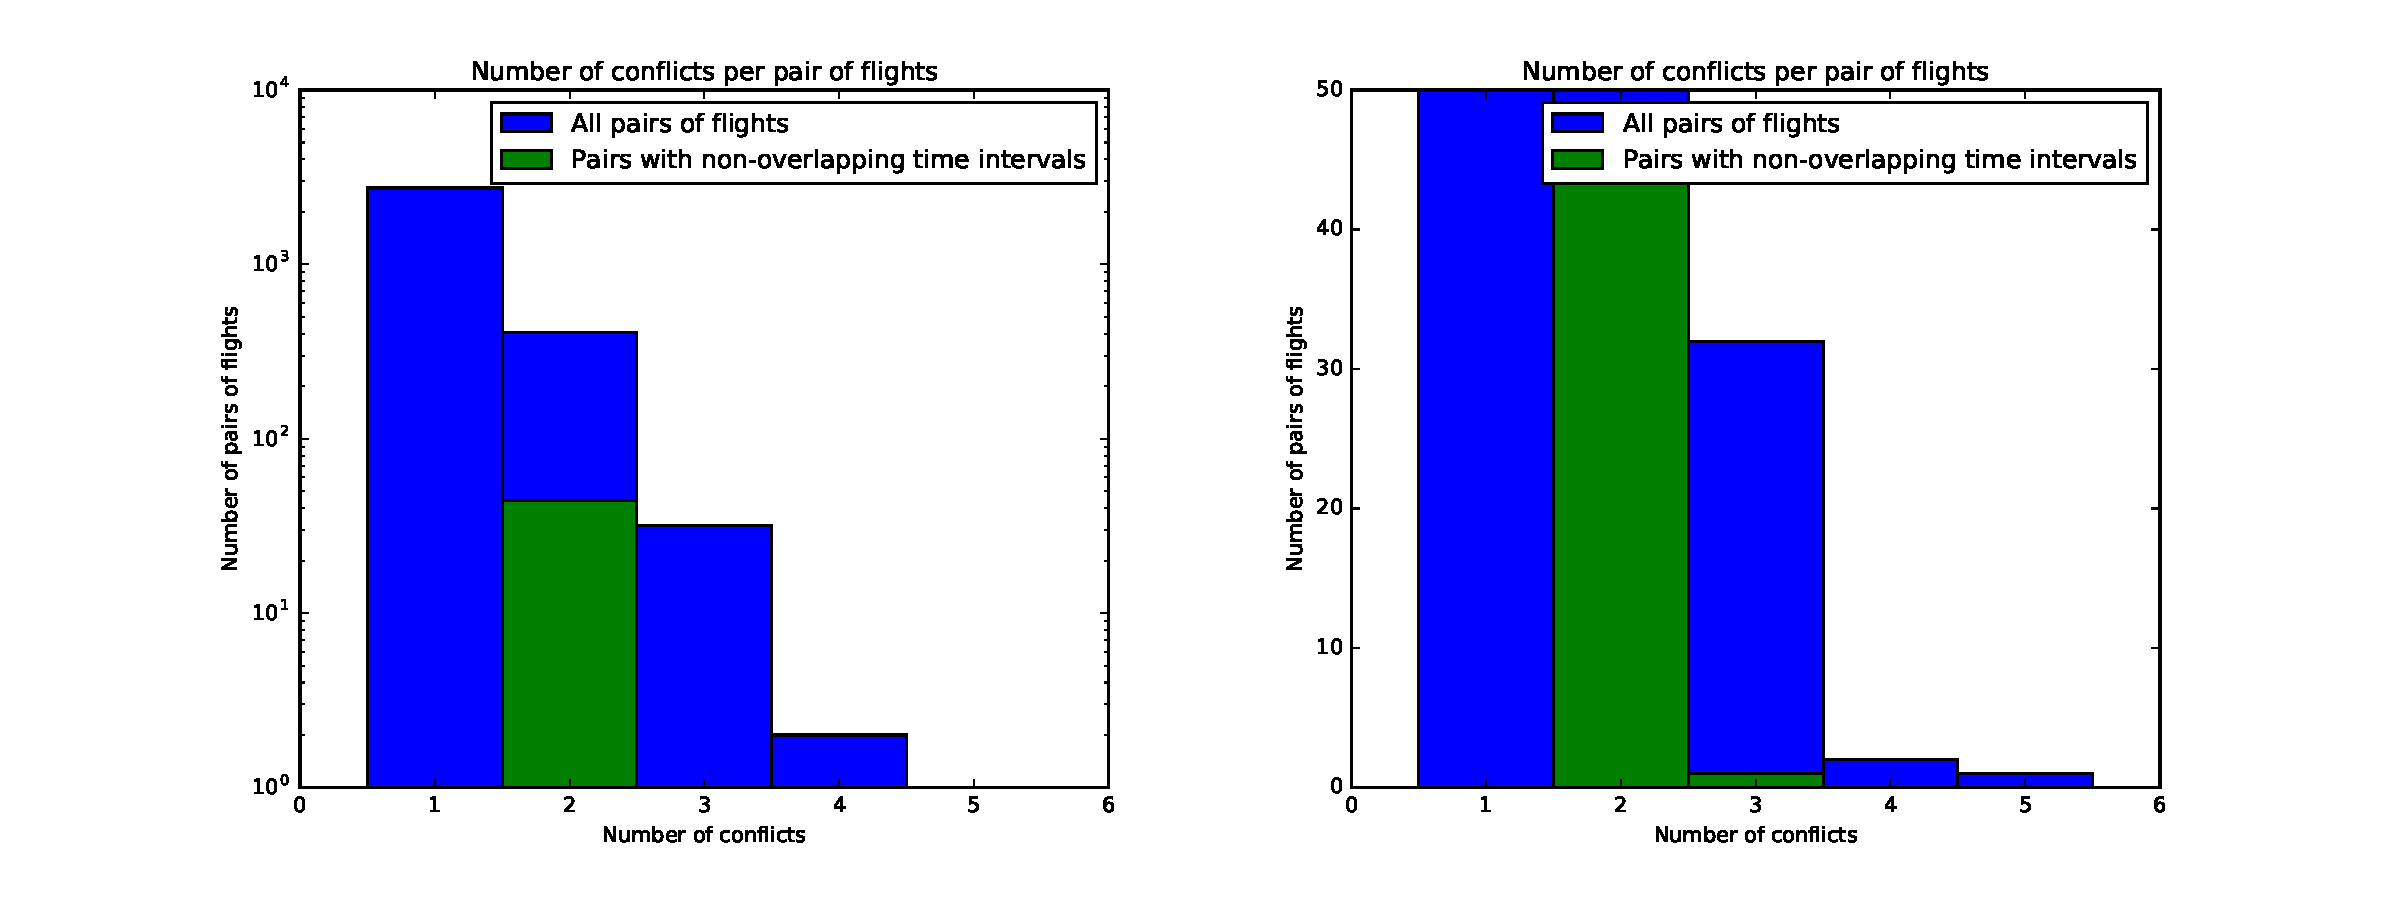
\includegraphics[width=1.0\linewidth]{pics/potential_conflicts_non_overlapping_time_intervals_statistics.pdf}
    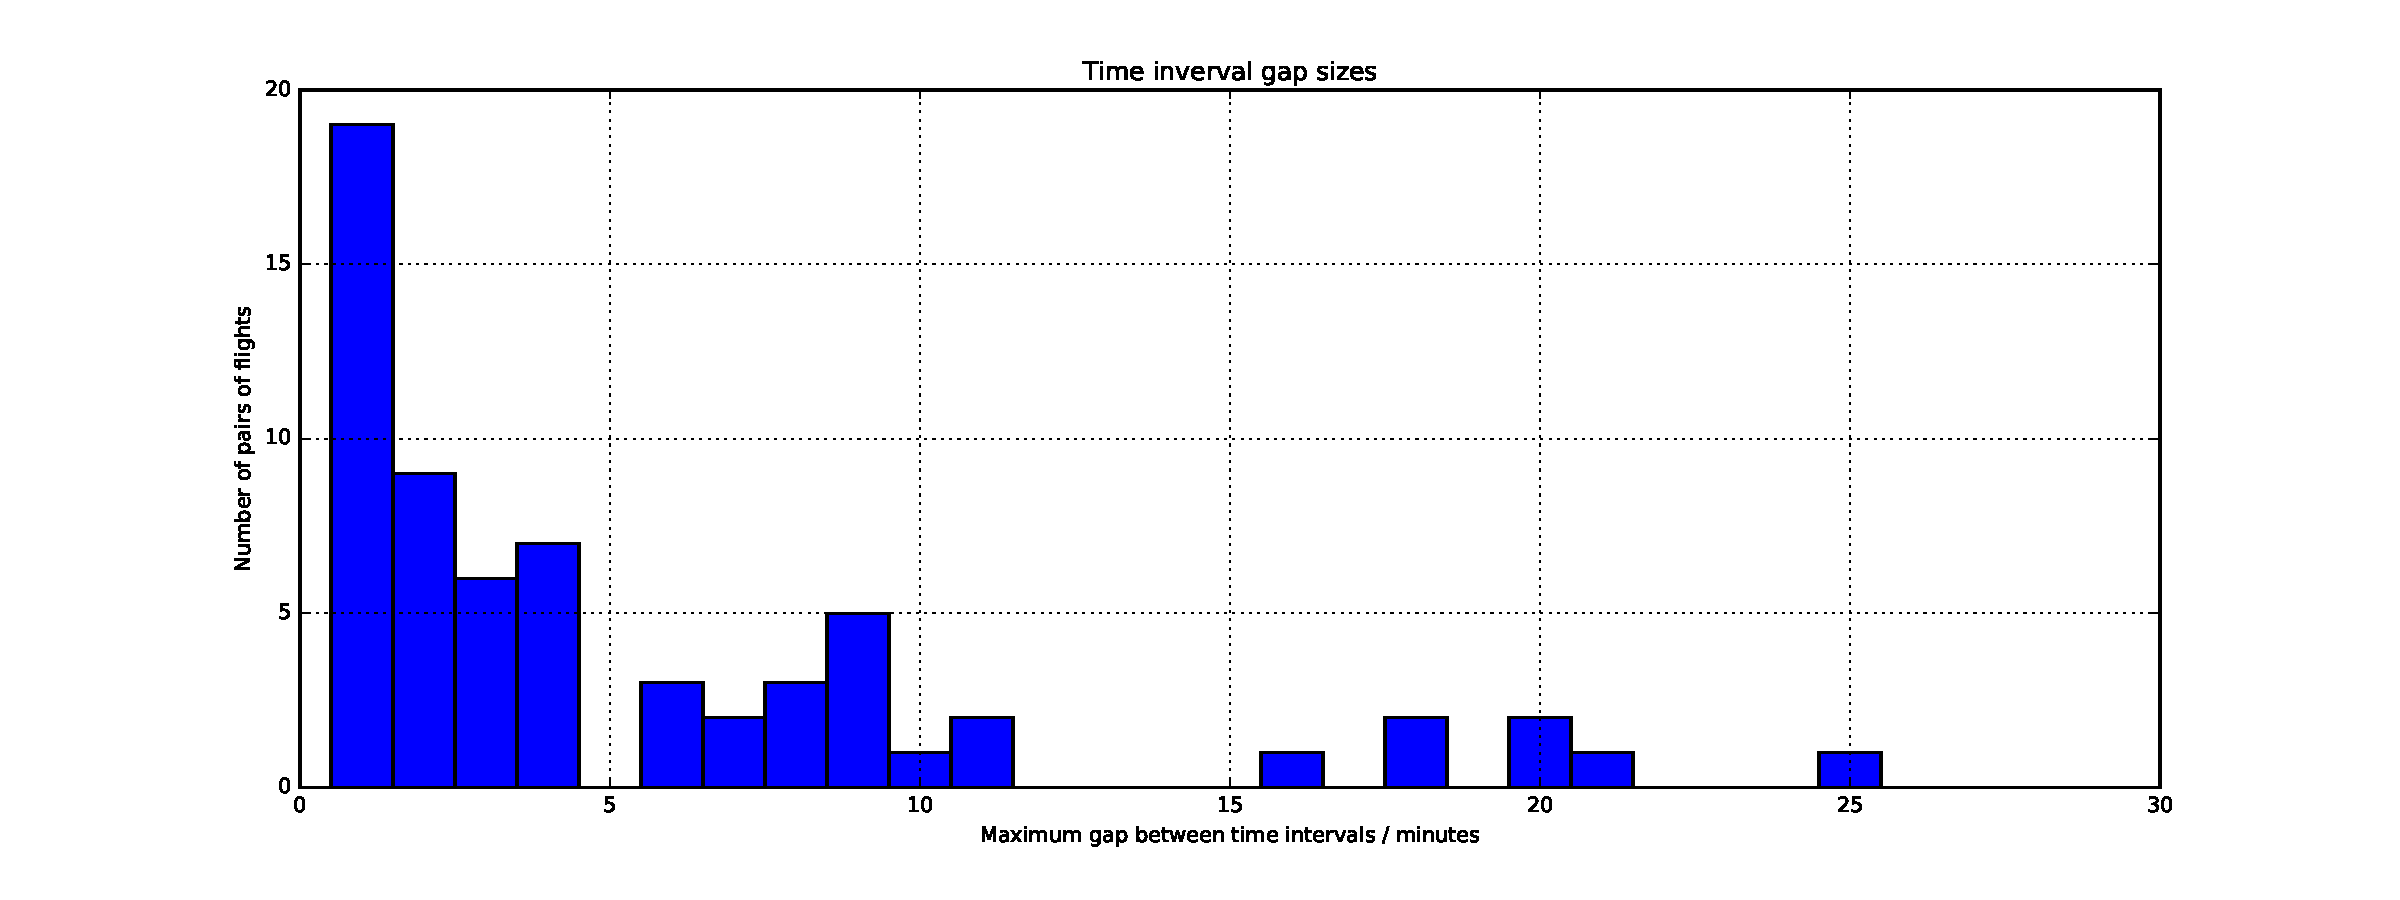
\includegraphics[width=1.0\linewidth]{pics/potential_conflicts_non_overlapping_time_intervals_gap_sizes.pdf}
    \caption{Top: Number of conflicts between pairs of flights. Bottom: Maximum gap sizes between non-overlapping conflict time intervals}
    \label{fig:pre_overlapping_time_intervals}
\end{figure}

Figure \ref{fig:pre_flight_pair_with_two_conflicts} shows an example of a pair of flights with two conflicts.
The two conflicts ($k=69$ and $k=70$) are between flights $i=10$ and $i=12$.
For the first conflict $k=69$ the time interval reads $[-8, -1]$ and for the second conflict $k=70$ it reads $[1, 7]$.
\begin{figure}[htpb]
    \centering
    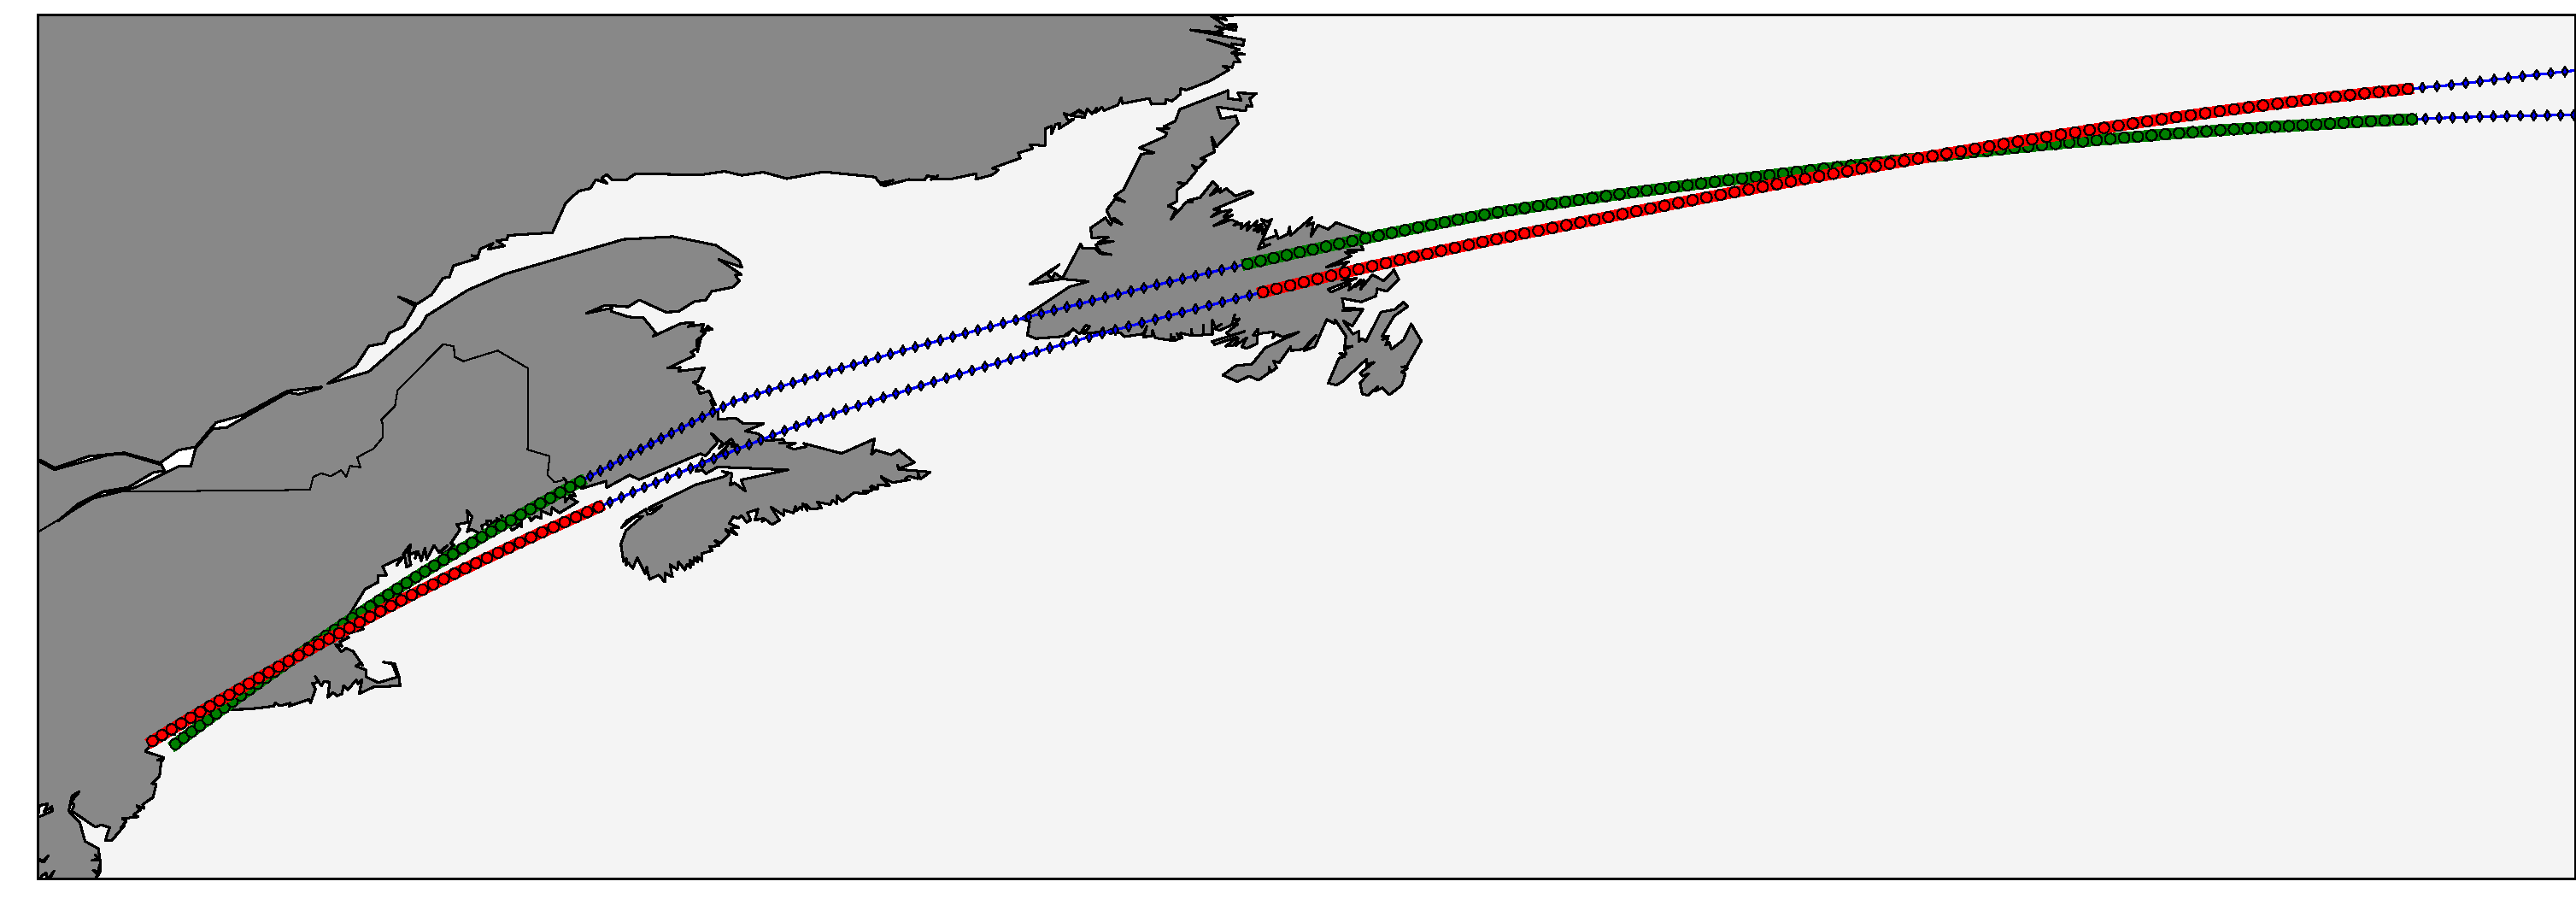
\includegraphics[width=1.0\linewidth]{pics/pre_flight_pair_with_two_conflicts.pdf}
    \caption{Example of two conflicts between two flights}
    \label{fig:pre_flight_pair_with_two_conflicts}
\end{figure}

In contrast, figure \ref{fig:pre_flight_pair_with_five_conflicts} shows a pair of flights with five conflicts.
The time interval reads $[-20, -20]$ for all five conflicts.
\begin{figure}[htpb]
    \centering
    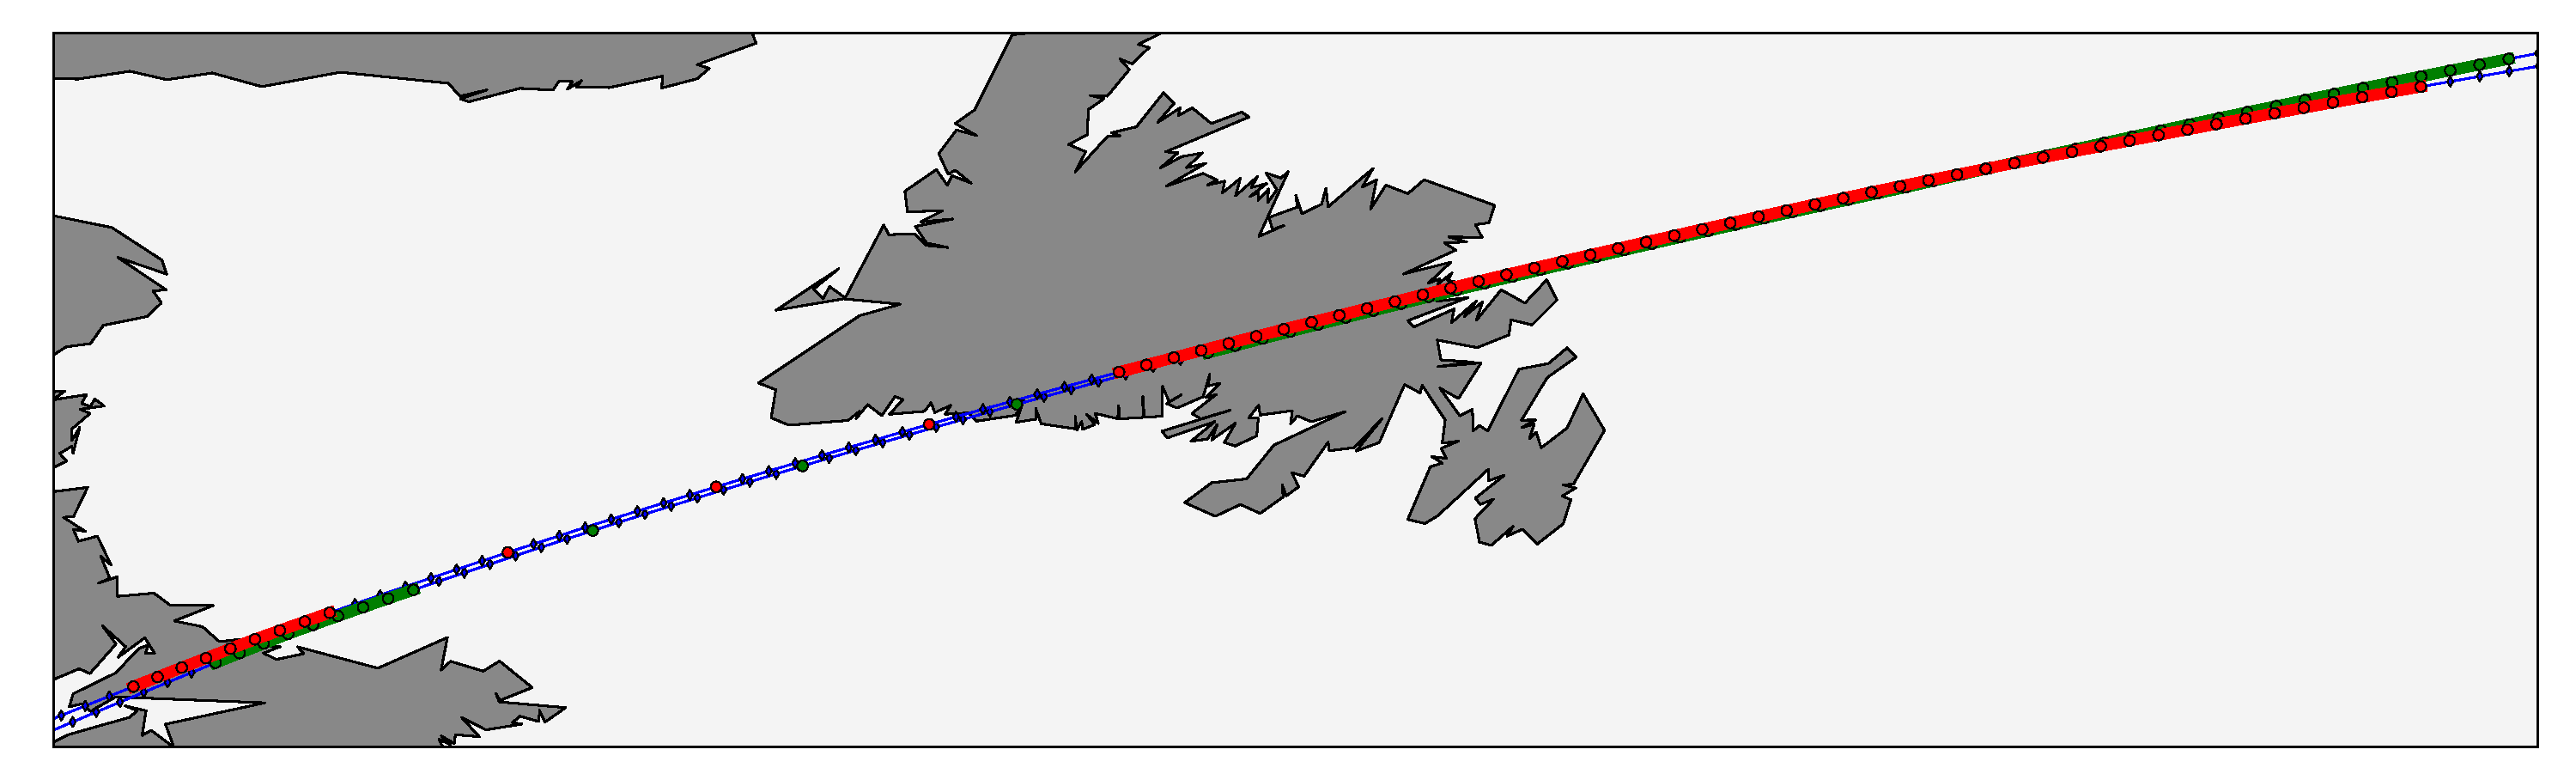
\includegraphics[width=1.0\linewidth]{pics/pre_flight_pair_with_five_conflicts.pdf}
    \caption{Example of five conflicts between two flights}
    \label{fig:pre_flight_pair_with_five_conflicts}
\end{figure}


\newpage
\section{Exact Solution of the Delay Only Model}
We want to investigate the influence of departure delay discretization in the delay only model.
Therefore we used a constraint programming solver to solve most of the connected component subsets of the problem.
\begin{figure}[htpb]
    \centering
    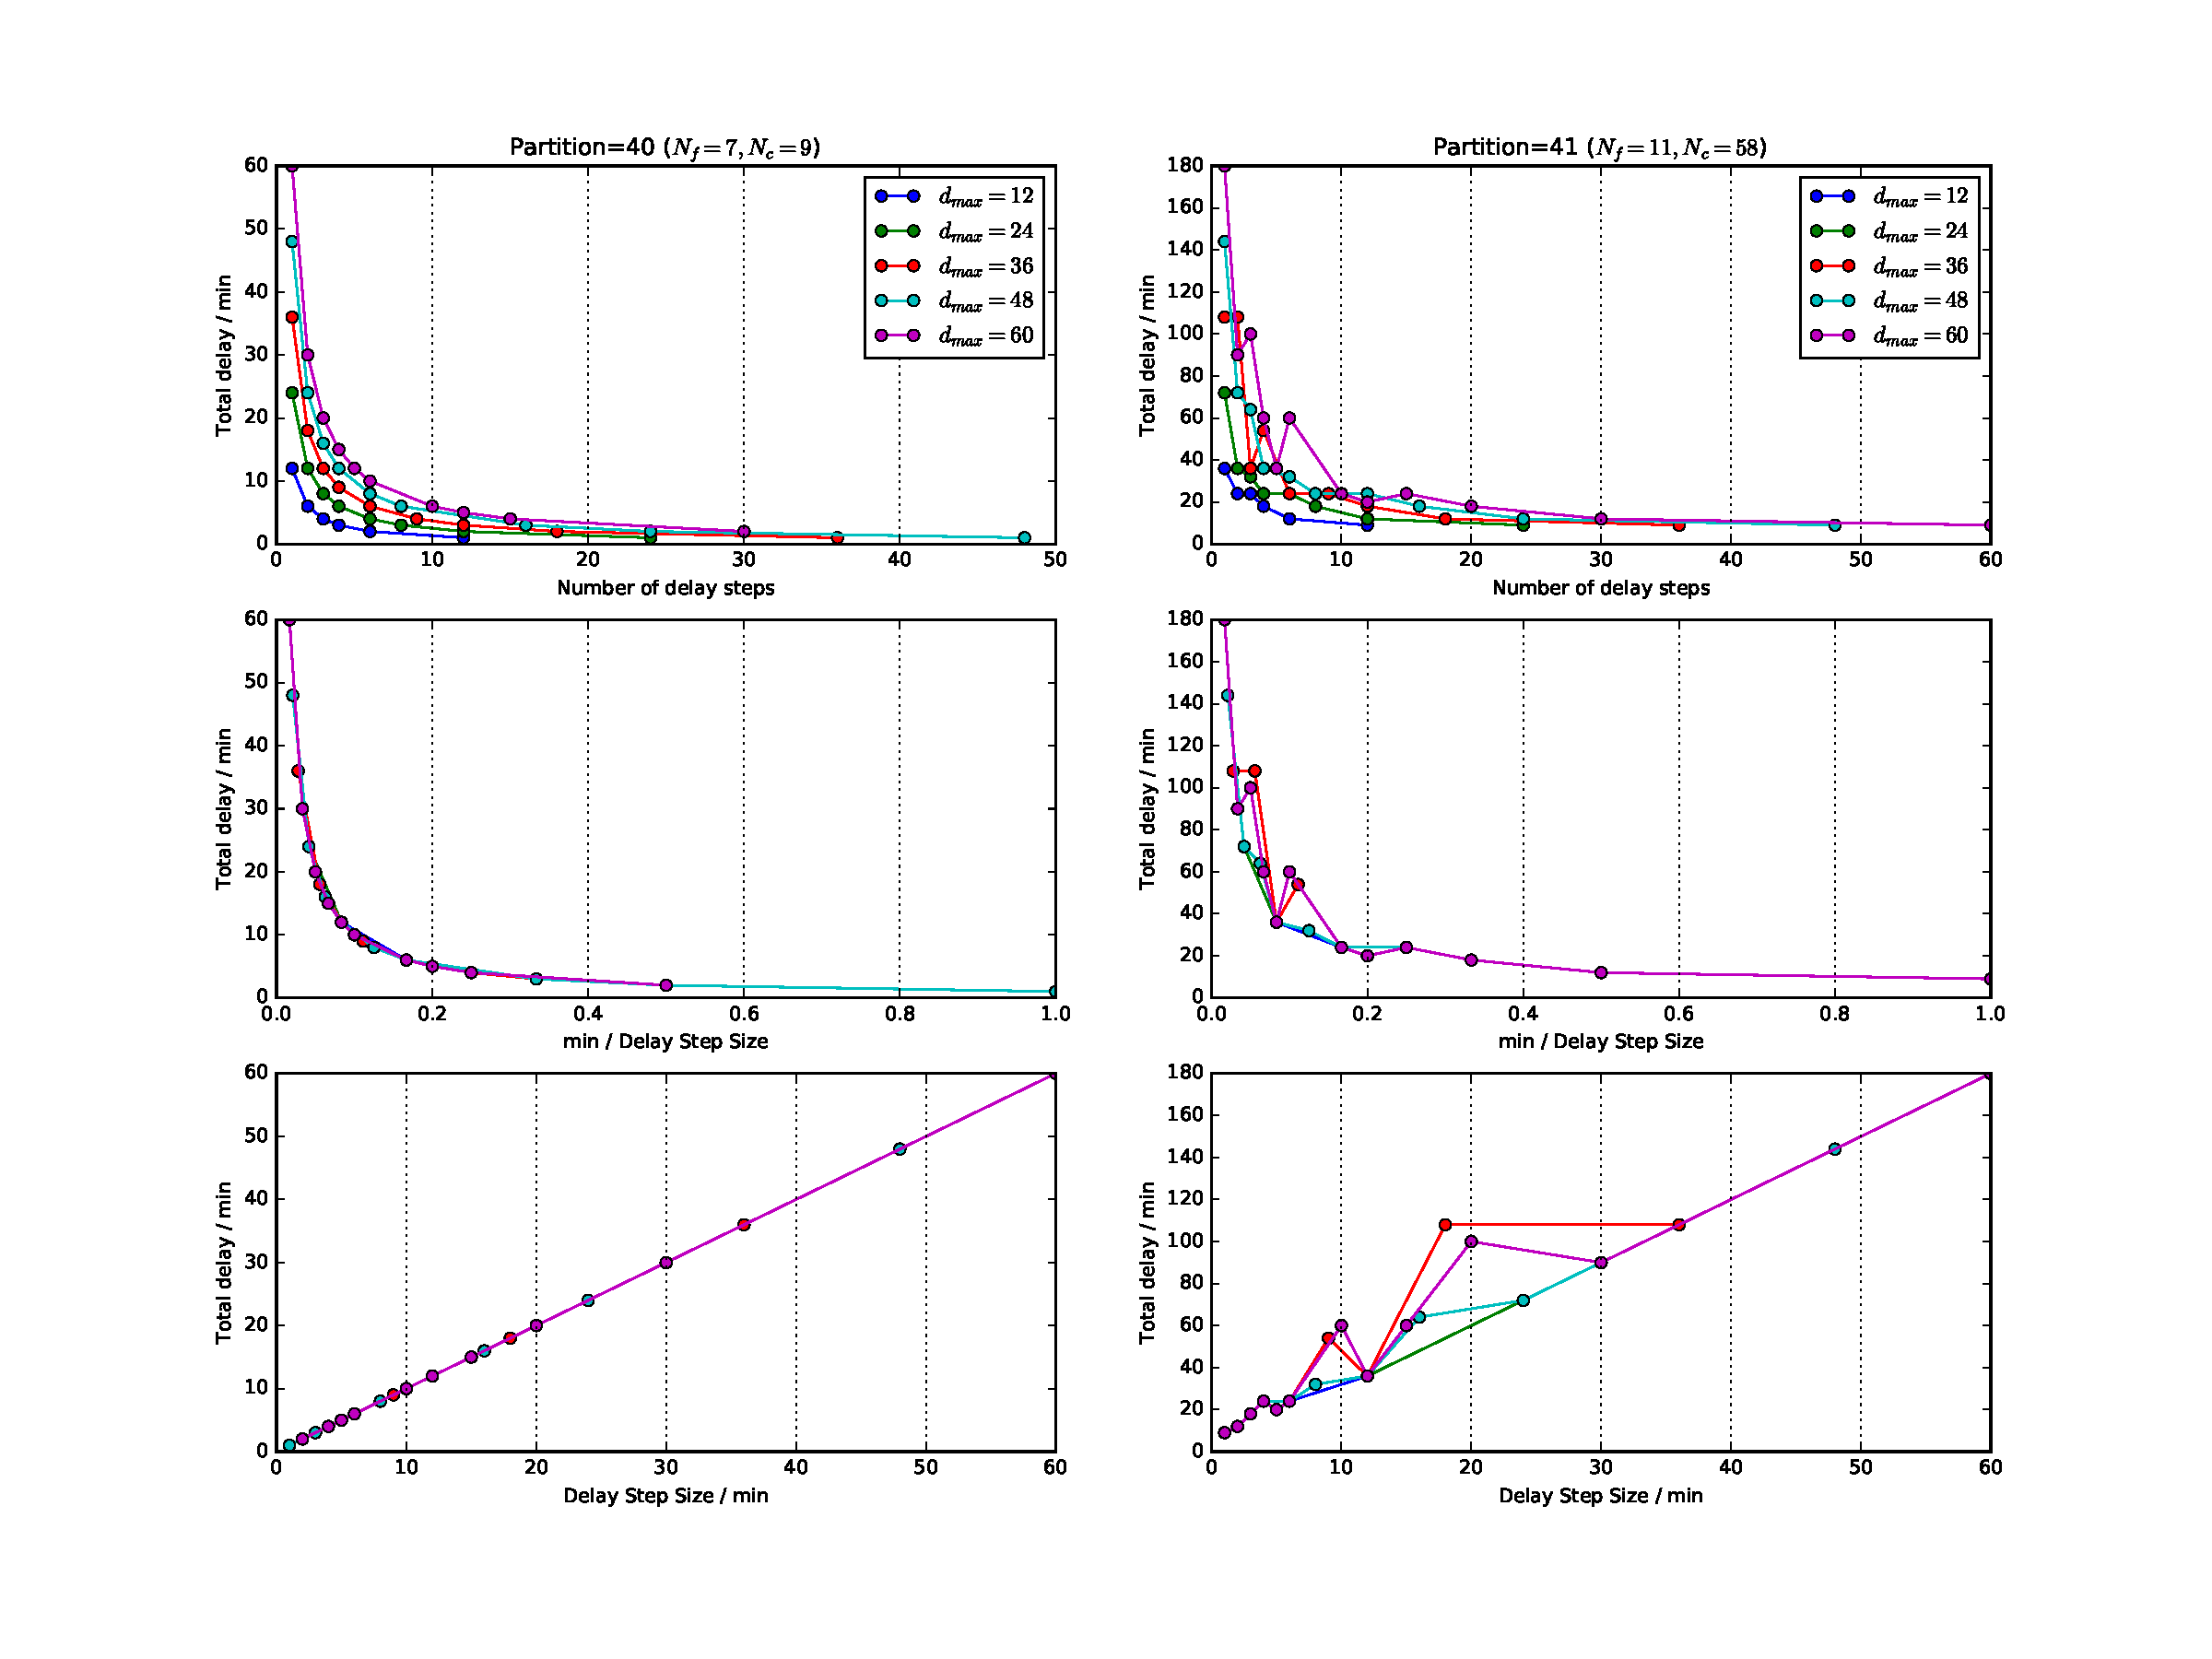
\includegraphics[width=1.0\linewidth]{pics/totalDelayVsDelayStep_examples.pdf}
    \caption{Influence of the discretization on the solution of the two instances extracted from connected components of the conflict graph}
    \label{fig:totalDelayVsDelayStep}
\end{figure}
Figure \ref{fig:totalDelayVsDelayStep} shows the total delay of the solution in dependence of the number of delay steps used.
We can see that a fairly low maximum delay step $d_\text{max}$ is sufficient.
On the other hand, the solutions get better for smaller the delay step sizes $\Delta d$.

\section{Exact Solution of the QUBO Formulation of the Delay Only Model}
The QUBO formulation of the problem requires the reformulation of constraints as additional penalty terms in the objective function.
If these penalty weights are chosen too large the original objective might get suppressed. 
On the other hand, if the penalty weights are too small the resulting solution can become invalid due to non-vanishing penalty terms.
Therefore we investigate the solution to the QUBO formulation of the delay only model checking the validity of the exact solution for various penalty weights.
In the course of this we used an algorithm which tracks the boundary between valid and invalid solutions.
Figure \ref{fig:validityMaps} shows an example for the validity of the solution in dependence of the penalty weights.
In all observed cases there is a box like shape of the validity boundary.
Moreover the validity boundary moves to higher penalty weights for decreasing number of delay steps.
\begin{figure}[htpb]
    \centering
    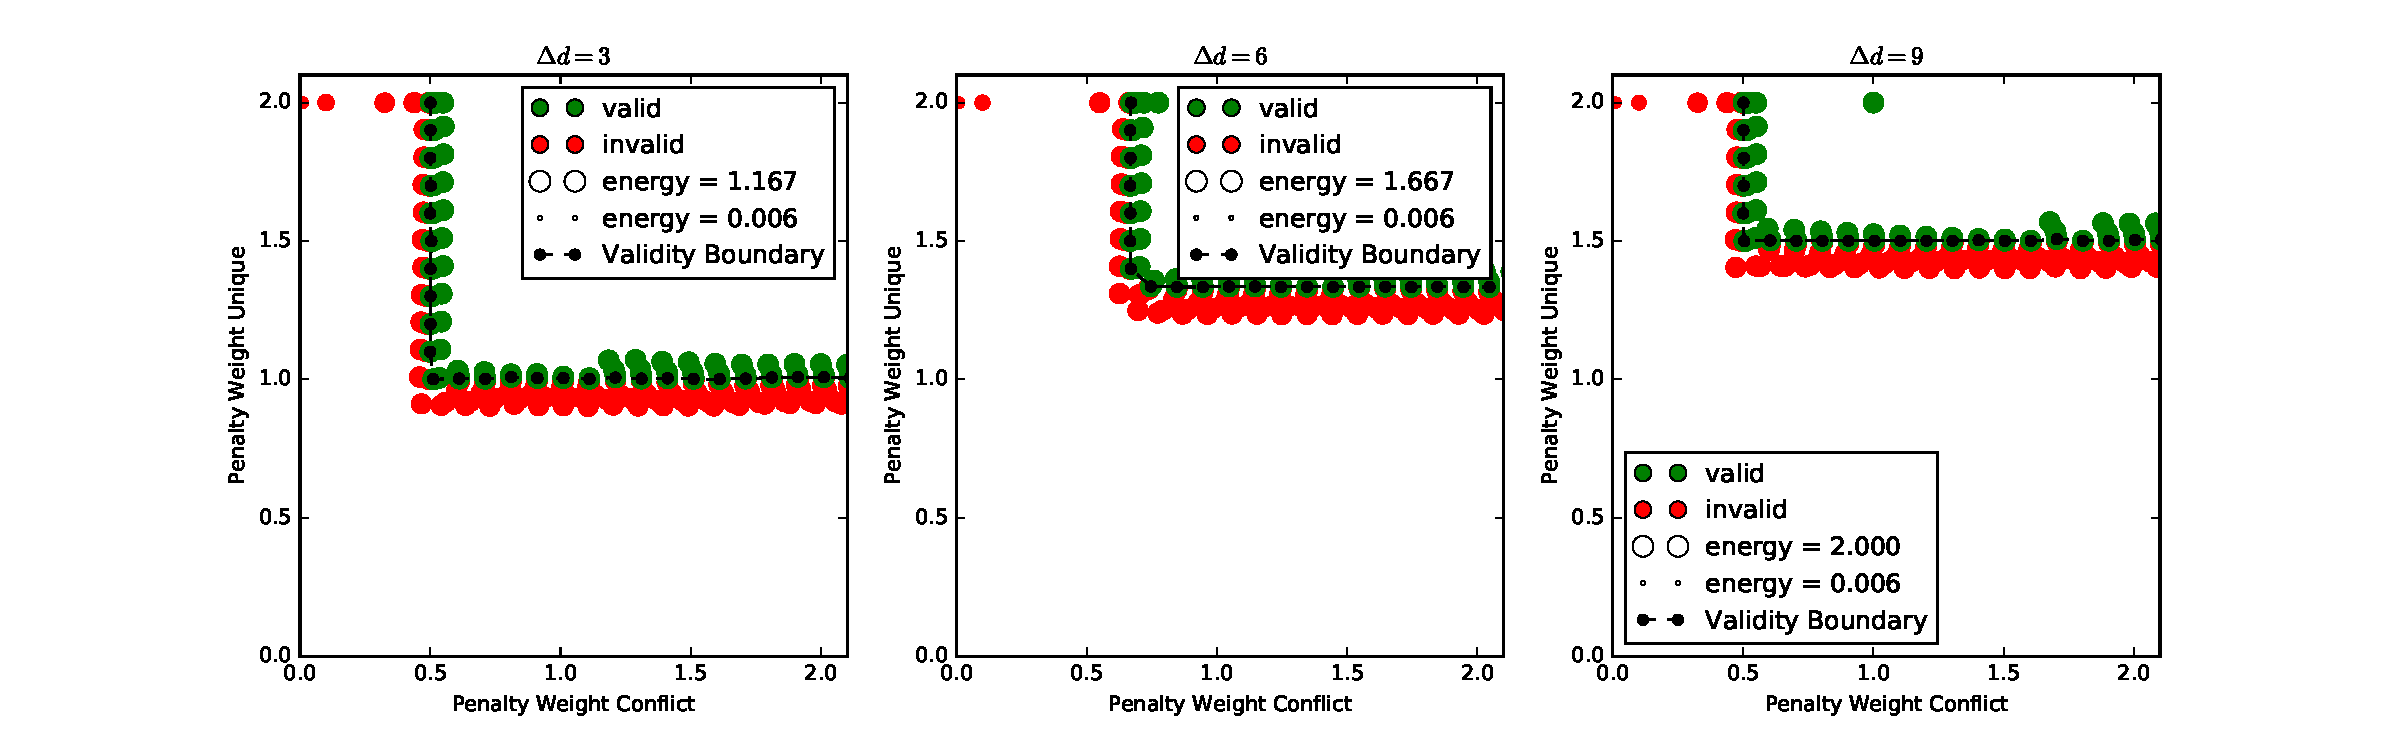
\includegraphics[width=1.0\linewidth]{pics/validity_maps_examples.pdf}
    \caption{Validity of the solution to the QUBO formulation of the delay only model in dependence of the penalty weights for various values of the delay step size $\Delta d$. The instance was extracted from partition 41 and $d_\text{max}=18$.}
    \label{fig:validityMaps}
\end{figure}
\section{Quantum Annealing Solution of the Delay Only Model}
So far, we solved the first 42 partitions with the quantum annealer.
We used 5 different embeddings and 10000 annealing runs per embedding.
As penalty weights we used $(\lambda_\text{unique}, \lambda_\text{conflict}) = \left\{(0.5, 0.5), (1, 1), (2, 2)\right\}$.

\begin{figure}[htpb]
    \centering
    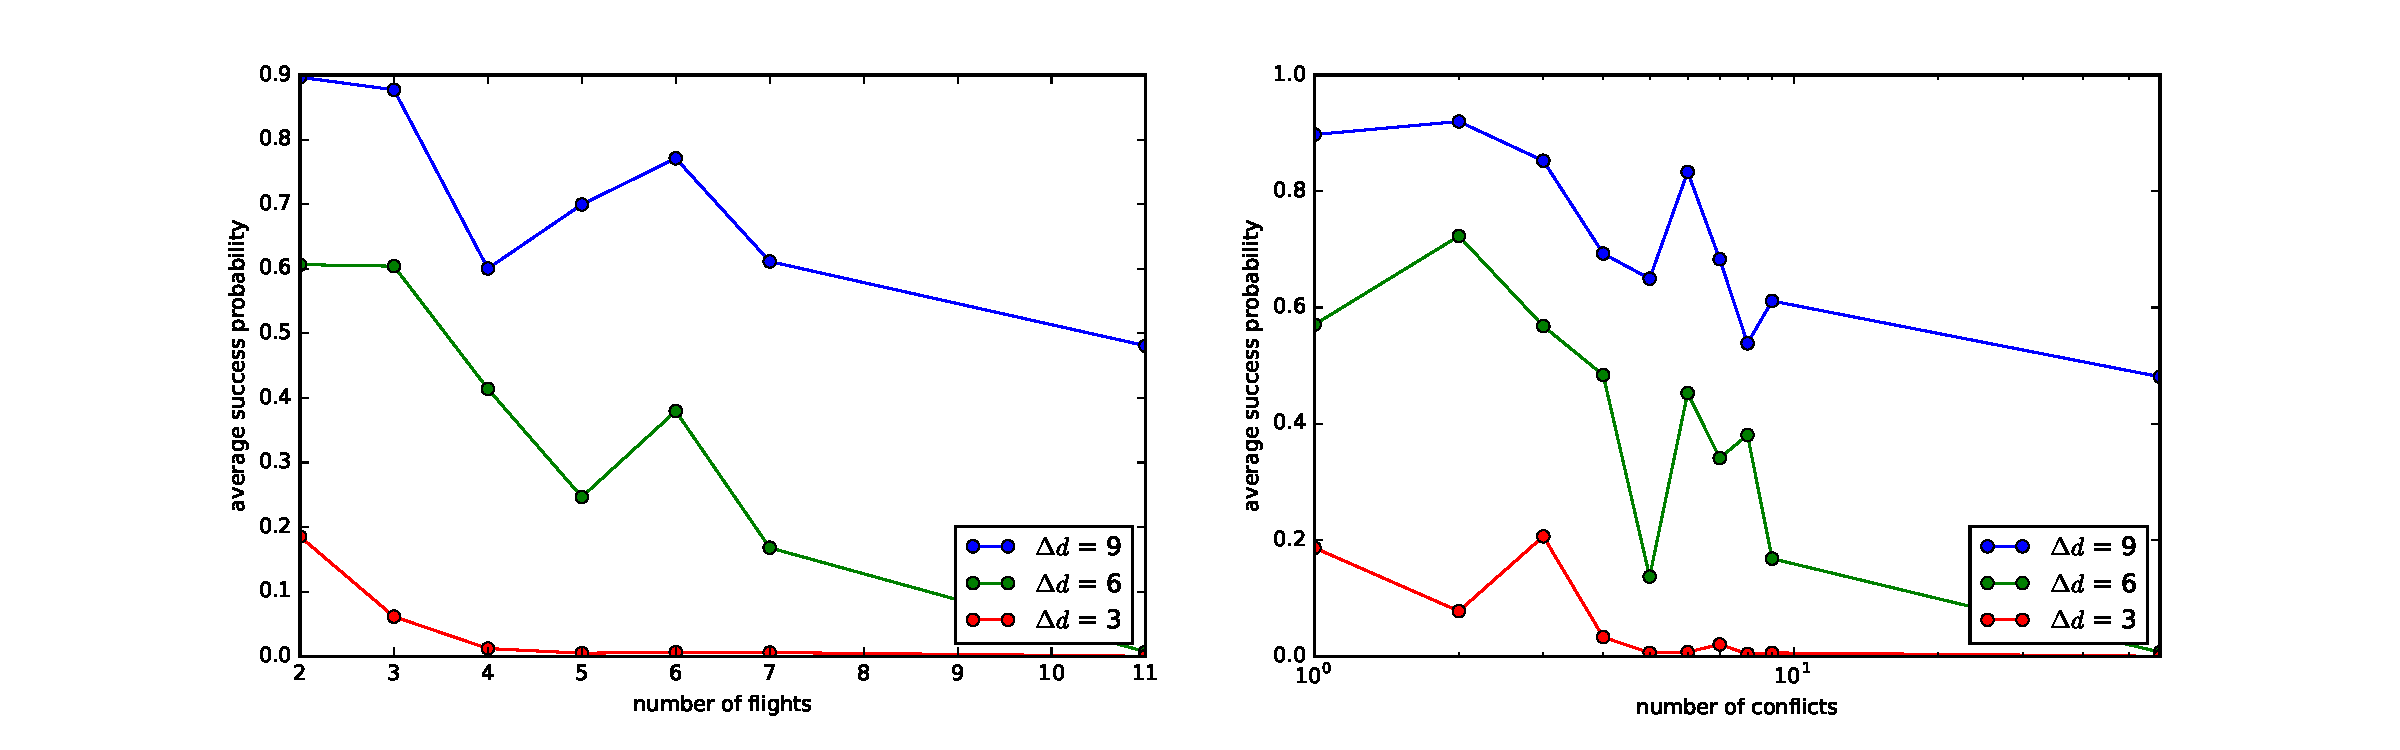
\includegraphics[width=1.0\linewidth]{pics/annealing_results_success_vs_flights_and_conflicts.pdf}
    \caption{Success probability versus number of flights and conflicts for various delay step sizes. The data includes the first 42 partitions of the conflict graph.}
    \label{fig:qa_success_vs_flights_and_conflicts}
\end{figure}

\begin{figure}[htpb]
    \centering
    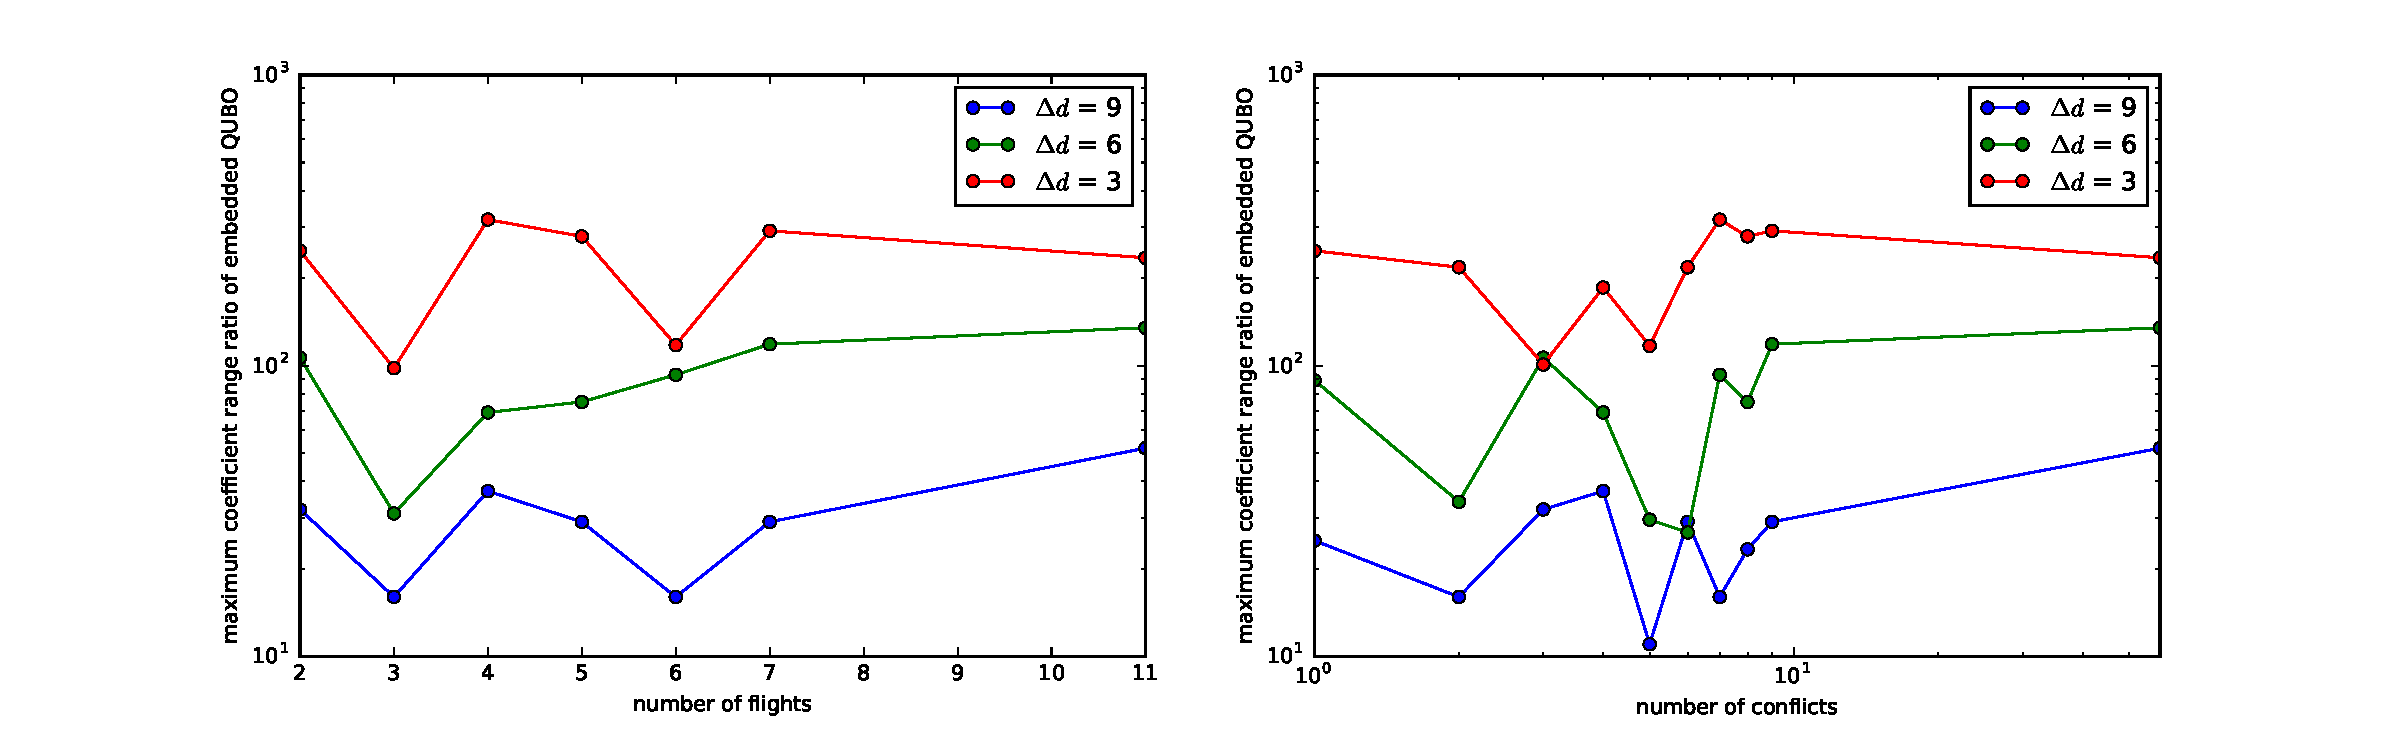
\includegraphics[width=1.0\linewidth]{pics/annealing_results_coefficent_range_ratio_vs_flights_and_conflicts.pdf}
    \caption{Maximum coefficient range ratio for number of flights and conflicts for various delay step sizes. The data includes the first 42 partitions of the conflict graph.}
    \label{fig:qa_coefficient_range_ratio_vs_flights_and_conflicts}
\end{figure}

\begin{figure}[htpb]
    \centering
    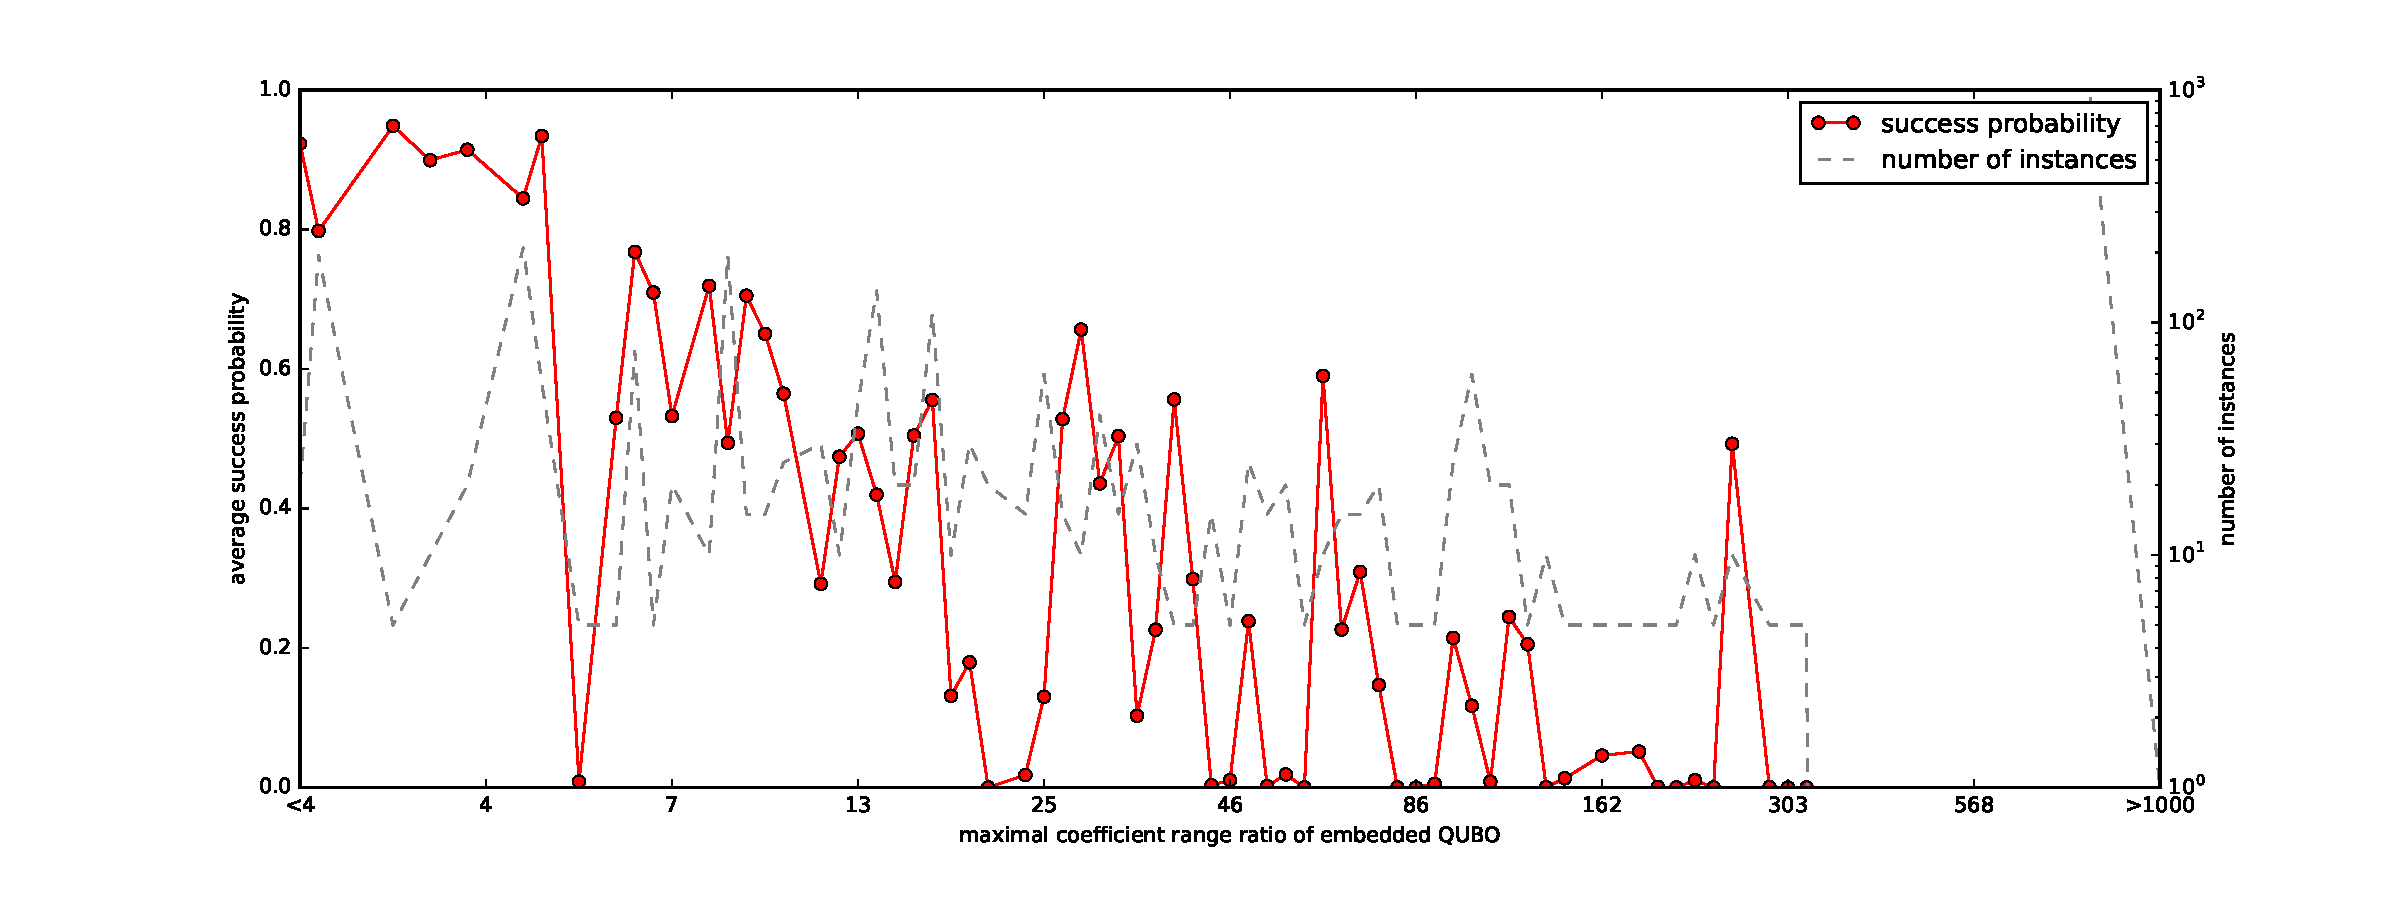
\includegraphics[width=1.0\linewidth]{pics/annealing_results_success_vs_cooefficent_range_ratio.pdf}
    \caption{Success probability versus the maximum coefficient range ratio. The data includes the first 42 partitions of the conflict graph.}
    \label{fig:qa_coefficient_range_ratio_vs_flights_and_conflicts}
\end{figure}
\end{document}
